% Options for packages loaded elsewhere
% Options for packages loaded elsewhere
\PassOptionsToPackage{unicode}{hyperref}
\PassOptionsToPackage{hyphens}{url}
\PassOptionsToPackage{dvipsnames,svgnames,x11names}{xcolor}
%
\documentclass[
  english,
  letterpaper,
  twoside,
  openright,
  10.5pt]{scrbook}
\usepackage{xcolor}
\usepackage[inner=0.92in,outer=0.76in,top=0.76in,bottom=0.86in,bindingoffset=0.12in,headheight=16pt,headsep=18pt,footskip=27pt]{geometry}
\usepackage{amsmath,amssymb}
\setcounter{secnumdepth}{5}
\usepackage{iftex}
\ifPDFTeX
  \usepackage[T1]{fontenc}
  \usepackage[utf8]{inputenc}
  \usepackage{textcomp} % provide euro and other symbols
\else % if luatex or xetex
  \usepackage{unicode-math} % this also loads fontspec
  \defaultfontfeatures{Scale=MatchLowercase}
  \defaultfontfeatures[\rmfamily]{Ligatures=TeX,Scale=1}
\fi
\usepackage{lmodern}
\ifPDFTeX\else
  % xetex/luatex font selection
\fi
% Use upquote if available, for straight quotes in verbatim environments
\IfFileExists{upquote.sty}{\usepackage{upquote}}{}
\IfFileExists{microtype.sty}{% use microtype if available
  \usepackage[]{microtype}
  \UseMicrotypeSet[protrusion]{basicmath} % disable protrusion for tt fonts
}{}
\makeatletter
\@ifundefined{KOMAClassName}{% if non-KOMA class
  \IfFileExists{parskip.sty}{%
    \usepackage{parskip}
  }{% else
    \setlength{\parindent}{0pt}
    \setlength{\parskip}{6pt plus 2pt minus 1pt}}
}{% if KOMA class
  \KOMAoptions{parskip=half}}
\makeatother
% Make \paragraph and \subparagraph free-standing
\makeatletter
\ifx\paragraph\undefined\else
  \let\oldparagraph\paragraph
  \renewcommand{\paragraph}{
    \@ifstar
      \xxxParagraphStar
      \xxxParagraphNoStar
  }
  \newcommand{\xxxParagraphStar}[1]{\oldparagraph*{#1}\mbox{}}
  \newcommand{\xxxParagraphNoStar}[1]{\oldparagraph{#1}\mbox{}}
\fi
\ifx\subparagraph\undefined\else
  \let\oldsubparagraph\subparagraph
  \renewcommand{\subparagraph}{
    \@ifstar
      \xxxSubParagraphStar
      \xxxSubParagraphNoStar
  }
  \newcommand{\xxxSubParagraphStar}[1]{\oldsubparagraph*{#1}\mbox{}}
  \newcommand{\xxxSubParagraphNoStar}[1]{\oldsubparagraph{#1}\mbox{}}
\fi
\makeatother

\usepackage{color}
\usepackage{fancyvrb}
\newcommand{\VerbBar}{|}
\newcommand{\VERB}{\Verb[commandchars=\\\{\}]}
\DefineVerbatimEnvironment{Highlighting}{Verbatim}{commandchars=\\\{\}}
% Add ',fontsize=\small' for more characters per line
\newenvironment{Shaded}{}{}
\newcommand{\AlertTok}[1]{\textcolor[rgb]{0.75,0.01,0.01}{\textbf{\colorbox[rgb]{0.97,0.90,0.90}{#1}}}}
\newcommand{\AnnotationTok}[1]{\textcolor[rgb]{0.79,0.38,0.79}{#1}}
\newcommand{\AttributeTok}[1]{\textcolor[rgb]{0.00,0.34,0.68}{#1}}
\newcommand{\BaseNTok}[1]{\textcolor[rgb]{0.69,0.50,0.00}{#1}}
\newcommand{\BuiltInTok}[1]{\textcolor[rgb]{0.39,0.29,0.61}{\textbf{#1}}}
\newcommand{\CharTok}[1]{\textcolor[rgb]{0.57,0.30,0.62}{#1}}
\newcommand{\CommentTok}[1]{\textcolor[rgb]{0.54,0.53,0.53}{#1}}
\newcommand{\CommentVarTok}[1]{\textcolor[rgb]{0.00,0.58,1.00}{#1}}
\newcommand{\ConstantTok}[1]{\textcolor[rgb]{0.67,0.33,0.00}{#1}}
\newcommand{\ControlFlowTok}[1]{\textcolor[rgb]{0.12,0.11,0.11}{\textbf{#1}}}
\newcommand{\DataTypeTok}[1]{\textcolor[rgb]{0.00,0.34,0.68}{#1}}
\newcommand{\DecValTok}[1]{\textcolor[rgb]{0.69,0.50,0.00}{#1}}
\newcommand{\DocumentationTok}[1]{\textcolor[rgb]{0.38,0.47,0.50}{#1}}
\newcommand{\ErrorTok}[1]{\textcolor[rgb]{0.75,0.01,0.01}{\underline{#1}}}
\newcommand{\ExtensionTok}[1]{\textcolor[rgb]{0.00,0.58,1.00}{\textbf{#1}}}
\newcommand{\FloatTok}[1]{\textcolor[rgb]{0.69,0.50,0.00}{#1}}
\newcommand{\FunctionTok}[1]{\textcolor[rgb]{0.39,0.29,0.61}{#1}}
\newcommand{\ImportTok}[1]{\textcolor[rgb]{1.00,0.33,0.00}{#1}}
\newcommand{\InformationTok}[1]{\textcolor[rgb]{0.69,0.50,0.00}{#1}}
\newcommand{\KeywordTok}[1]{\textcolor[rgb]{0.12,0.11,0.11}{\textbf{#1}}}
\newcommand{\NormalTok}[1]{\textcolor[rgb]{0.12,0.11,0.11}{#1}}
\newcommand{\OperatorTok}[1]{\textcolor[rgb]{0.79,0.38,0.79}{#1}}
\newcommand{\OtherTok}[1]{\textcolor[rgb]{0.00,0.43,0.16}{#1}}
\newcommand{\PreprocessorTok}[1]{\textcolor[rgb]{0.00,0.43,0.16}{#1}}
\newcommand{\RegionMarkerTok}[1]{\textcolor[rgb]{0.00,0.34,0.68}{\colorbox[rgb]{0.88,0.91,0.97}{#1}}}
\newcommand{\SpecialCharTok}[1]{\textcolor[rgb]{0.24,0.68,0.91}{#1}}
\newcommand{\SpecialStringTok}[1]{\textcolor[rgb]{1.00,0.33,0.00}{#1}}
\newcommand{\StringTok}[1]{\textcolor[rgb]{0.75,0.01,0.01}{#1}}
\newcommand{\VariableTok}[1]{\textcolor[rgb]{0.00,0.34,0.68}{#1}}
\newcommand{\VerbatimStringTok}[1]{\textcolor[rgb]{0.75,0.01,0.01}{#1}}
\newcommand{\WarningTok}[1]{\textcolor[rgb]{0.75,0.01,0.01}{#1}}

\usepackage{longtable,booktabs,array}
\usepackage{calc} % for calculating minipage widths
% Correct order of tables after \paragraph or \subparagraph
\usepackage{etoolbox}
\makeatletter
\patchcmd\longtable{\par}{\if@noskipsec\mbox{}\fi\par}{}{}
\makeatother
% Allow footnotes in longtable head/foot
\IfFileExists{footnotehyper.sty}{\usepackage{footnotehyper}}{\usepackage{footnote}}
\makesavenoteenv{longtable}
\usepackage{graphicx}
\makeatletter
\newsavebox\pandoc@box
\newcommand*\pandocbounded[1]{% scales image to fit in text height/width
  \sbox\pandoc@box{#1}%
  \Gscale@div\@tempa{\textheight}{\dimexpr\ht\pandoc@box+\dp\pandoc@box\relax}%
  \Gscale@div\@tempb{\linewidth}{\wd\pandoc@box}%
  \ifdim\@tempb\p@<\@tempa\p@\let\@tempa\@tempb\fi% select the smaller of both
  \ifdim\@tempa\p@<\p@\scalebox{\@tempa}{\usebox\pandoc@box}%
  \else\usebox{\pandoc@box}%
  \fi%
}
% Set default figure placement to htbp
\def\fps@figure{htbp}
\makeatother



\ifLuaTeX
\usepackage[bidi=basic]{babel}
\else
\usepackage[bidi=default]{babel}
\fi
% get rid of language-specific shorthands (see #6817):
\let\LanguageShortHands\languageshorthands
\def\languageshorthands#1{}
\ifLuaTeX
  \usepackage[english]{selnolig} % disable illegal ligatures
\fi


\setlength{\emergencystretch}{3em} % prevent overfull lines

\providecommand{\tightlist}{%
  \setlength{\itemsep}{0pt}\setlength{\parskip}{0pt}}



 


% Deep Learning print palette. Line/shape differences preserve grayscale meaning.
\usepackage{xcolor}
\definecolor{DLNavy}{HTML}{081B33}
\definecolor{DLIndigo}{HTML}{263F8F}
\definecolor{DLBlue}{HTML}{3157D5}
\definecolor{DLCyan}{HTML}{238BA8}
\definecolor{DLSlate}{HTML}{5B6678}
\definecolor{DLLight}{HTML}{F4F7FA}
\definecolor{DLMid}{HTML}{D7DEE8}
\definecolor{DLCharcoal}{HTML}{202833}
\definecolor{DLCodeBg}{HTML}{F1F4F8}
% Open fonts distributed with TeX Live; no font binaries are committed.
\usepackage{fontspec}
\setmainfont{TeX Gyre Pagella}[Ligatures=TeX,Numbers=OldStyle]
\setsansfont{TeX Gyre Heros}[Scale=0.92,Ligatures=TeX]
\setmonofont{Latin Modern Mono}[Scale=0.88]
\usepackage{microtype}
\microtypesetup{protrusion=true,expansion=true,tracking=true}
\usepackage{needspace}
\usepackage{ragged2e}
\usepackage{setspace}
\AtBeginDocument{%
  \fontsize{10.6pt}{13.6pt}\selectfont
  \setlength{\parindent}{1.2em}
  \setlength{\parskip}{0.18em plus 0.06em minus 0.03em}
  \setlength{\emergencystretch}{2em}
  \clubpenalty=10000
  \widowpenalty=10000
  \displaywidowpenalty=10000
  \brokenpenalty=8000
  \predisplaypenalty=150
  \postdisplaypenalty=150
}
\usepackage{fancyhdr}
\usepackage{etoolbox}
\usepackage{bookmark}

\newcommand{\DLShortTitle}{DEEP LEARNING}
\newcommand{\DLEdition}{FIRST OPEN EDITION · 2026}

\fancypagestyle{dlbook}{%
  \fancyhf{}
  \fancyhead[LE]{\sffamily\fontsize{7.8}{9.2}\selectfont\bfseries\color{DLIndigo}\leftmark}
  \fancyhead[RO]{\sffamily\fontsize{7.8}{9.2}\selectfont\bfseries\color{DLSlate}\DLShortTitle{} · \DLEdition}
  \fancyfoot[LE]{\sffamily\color{DLBlue}\bfseries\thepage\hfill\color{DLSlate}\fontsize{7.6}{9}\selectfont Deep Learning: A Comprehensive Guide}
  \fancyfoot[RO]{\sffamily\color{DLSlate}\fontsize{7.6}{9}\selectfont Deep Learning: A Comprehensive Guide\hfill\color{DLBlue}\bfseries\thepage}
  \renewcommand{\headrulewidth}{0.35pt}
  \renewcommand{\footrulewidth}{0.25pt}
  \renewcommand{\headrule}{\hbox to\headwidth{\color{DLMid}\leaders\hrule height \headrulewidth\hfill}}
  \renewcommand{\footrule}{\hbox to\headwidth{\color{DLMid}\leaders\hrule height \footrulewidth\hfill}}
}
\pagestyle{dlbook}
\renewcommand{\chaptermark}[1]{\markboth{CHAPTER \ifnum\value{chapter}<10 0\fi\thechapter{} · \MakeUppercase{#1}}{}}
\renewcommand{\sectionmark}[1]{}

% Intentional blank versos remain completely blank.
\renewcommand{\cleardoublepage}{\clearpage\ifodd\value{page}\else\thispagestyle{empty}\hbox{}\newpage\fi}
\usepackage{tikz}
\usetikzlibrary{calc,positioning}
\usepackage[most]{tcolorbox}
\usepackage{enumitem}
\usepackage{titlesec}
\usepackage{etoolbox}

% Quarto title and part commands are replaced by designed print structures.
\AtBeginDocument{\renewcommand{\maketitle}{}}

% Layered representation motif: transformations compress toward an abstraction.
\newcommand{\DLLayers}[1]{%
  \begin{scope}[shift={(#1)}]
    \foreach \x/\op in {0/.12,.34/.16,.68/.20,1.02/.24,1.36/.30}{%
      \draw[DLCyan,opacity=\op,line width=.8pt] (\x in,0) rectangle ++(.22in,1.45in);}
    \draw[DLCyan,opacity=.35,line width=1.1pt,->] (0in,.72in)--(1.72in,.72in);
    \fill[DLCyan,opacity=.42] (1.82in,.72in) circle (4pt);
  \end{scope}}

\newcommand{\DLHalfTitle}{%
  \cleardoublepage\thispagestyle{empty}
  \vspace*{2.25in}
  {\centering\sffamily\bfseries\fontsize{31}{36}\selectfont\color{DLNavy}Deep Learning:\\A Comprehensive Guide\par}
  \vspace{.55in}{\centering\color{DLCyan}\rule{1.2in}{2pt}\par}
  \clearpage
}

\newcommand{\DLFullTitle}{%
  \thispagestyle{empty}%
  \begin{tikzpicture}[remember picture,overlay]
    \fill[DLNavy] ([xshift=.76in,yshift=.86in]current page.south west) rectangle ([xshift=-1.04in,yshift=-.76in]current page.north east);
    \DLLayers{[xshift=-3.29in,yshift=-2.91in]current page.north east}
  \end{tikzpicture}%
  \vspace*{.68in}\begin{minipage}[t][.82\textheight][t]{.86\textwidth}
    {\sffamily\bfseries\fontsize{35}{40}\selectfont\color{white}Deep Learning:\\A Comprehensive Guide\par}
    \vspace{.7em}{\color{DLCyan}\rule{1.55in}{2.4pt}\par}
    \vspace{.65em}
    {\fontsize{16}{20}\selectfont\color{DLLight}Architectures, Training, Generative Models,\\and Real-World AI Systems\par}
    \vfill
    {\sffamily\bfseries\fontsize{15}{18}\selectfont\color{white}Moody Amakobe\par}
    \vspace{.55em}{\sffamily\fontsize{9}{11}\selectfont\color{DLCyan}FIRST OPEN EDITION · 2026 · CC BY 4.0\par}
  \end{minipage}\clearpage
}

\newcommand{\DLCopyrightPage}{%
  \thispagestyle{empty}\vspace*{.85in}
  {\sffamily\bfseries\fontsize{18}{22}\selectfont\color{DLNavy}Deep Learning: A Comprehensive Guide\par}
  \vspace{.25em}{\itshape Architectures, Training, Generative Models, and Real-World AI Systems\par}
  \vspace{1.1em}Moody Amakobe\par
  \vspace{1.25em}Copyright © 2026 Moody Amakobe\par
  \vspace{.8em}\textbf{First Open Edition}\par
  Independently published as an Open Educational Resource.\par
  \vspace{.9em}This work is licensed under the Creative Commons Attribution 4.0 International License unless otherwise indicated. You may share and adapt it with appropriate attribution, a license link, and an indication of changes.\par
  \vspace{.9em}ISBN — Print: To be assigned\\ISBN — PDF: To be assigned\\ISBN — EPUB: To be assigned\par
  \vspace{.9em}Deep learning frameworks, APIs, model behavior, software libraries, hardware, and deployment practices evolve rapidly. Readers implementing production systems should verify current technical documentation, test behavior in their target environment, and apply appropriate security, safety, legal, and professional review.\par
  \vfill{\small Recommended citation: Amakobe, M. (2026). \textit{Deep learning: A comprehensive guide: Architectures, training, generative models, and real-world AI systems} (First Open Edition).}\par
  \clearpage
}

\newcommand{\DLPrintContents}{%
  \setcounter{tocdepth}{1}%
  \cleardoublepage\pdfbookmark[0]{Contents}{contents}\tableofcontents
  \cleardoublepage\pdfbookmark[0]{List of Figures}{figures}\listoffigures
  \cleardoublepage
}

\newcommand{\DLPartOpener}[3]{%
  \cleardoublepage\refstepcounter{part}\addcontentsline{toc}{part}{\protect\numberline{\Roman{part}}#1}\thispagestyle{empty}
  \begin{tikzpicture}[remember picture,overlay]
    \fill[DLNavy] ([xshift=1.04in,yshift=.86in]current page.south west) rectangle ([xshift=-.76in,yshift=-.76in]current page.north east);
    \DLLayers{[xshift=-3.01in,yshift=-2.76in]current page.north east}
  \end{tikzpicture}%
  \vspace*{.3in}\begin{minipage}[t][.80\textheight][t]{.88\textwidth}
    {\sffamily\bfseries\fontsize{11}{13}\selectfont\color{DLCyan}PART\par}
    {\sffamily\bfseries\fontsize{72}{76}\selectfont\color{white}\Roman{part}\par}
    \vspace{.75in}{\sffamily\bfseries\fontsize{28}{33}\selectfont\color{white}#1\par}
    \vspace{.55em}{\color{DLCyan}\rule{1.35in}{2.2pt}\par}
    \vspace{.65em}{\fontsize{13}{17}\selectfont\color{DLLight}#2\par}
    \vspace{.7em}{\fontsize{10.5}{14}\selectfont\color{DLMid}#3\par}
  \end{minipage}\clearpage
}

% Quarto injects \part after Pandoc filters have run. Route those late-bound
% commands through the print design and consume the duplicate part-QMD prose
% up to the already-designed chapter opener.
\newif\ifDLContentsPrinted\DLContentsPrintedfalse
\long\def\DLDiscardPartText#1\DLChapterOpener#2#3#4#5{\DLChapterOpener{#2}{#3}{#4}{#5}}
\renewcommand{\part}[1]{%
  \ifDLContentsPrinted\end{DLSectionPanel}\else\DLPrintContents\DLStartMainMatter\global\DLContentsPrintedtrue\fi
  \ifstrequal{#1}{Foundations of Deep Learning}{\DLPartOpener{#1}{Deep learning begins with a deceptively simple idea: layered computation can learn useful representations directly from data.}{Neural computation, network architecture, and training practice establish the vocabulary used throughout the book.}}{}%
  \ifstrequal{#1}{Vision Systems}{\DLPartOpener{#1}{Vision systems transform spatial structure into increasingly abstract feature maps, predictions, and decisions.}{Convolution, attention, detection, segmentation, transfer learning, and pipeline evaluation form a connected visual-learning system.}}{}%
  \ifstrequal{#1}{Sequence, Language, and Multimodal Learning}{\DLPartOpener{#1}{Sequences introduce memory; attention makes relationships directly accessible; multimodal learning asks different representations to share meaning.}{Recurrent models lead to Transformers, pre-trained language models, and shared vision-language representations.}}{}%
  \ifstrequal{#1}{Generative and Adaptive Systems}{\DLPartOpener{#1}{Deep models can learn distributions, construct new samples, and adapt behavior through feedback.}{Variational, adversarial, diffusion, and reinforcement-learning systems expose complementary approaches to creation and adaptation.}}{}%
  \ifstrequal{#1}{Engineering and Responsible Deep Learning}{\DLPartOpener{#1}{A model becomes consequential when it enters a system.}{Deployment introduces drift, dependencies, scale, governance, professional responsibility, and human impact.}}{}%
  \DLDiscardPartText
}

\newcommand{\DLChapterOpener}[4]{%
  \cleardoublepage\refstepcounter{chapter}\addcontentsline{toc}{chapter}{\protect\numberline{\thechapter}#2}\chaptermark{#2}\thispagestyle{empty}
  \begin{tikzpicture}[remember picture,overlay]
    \fill[DLNavy] ([xshift=1.04in,yshift=-.76in]current page.north west) rectangle ([xshift=-.76in,yshift=-3.42in]current page.north east);
    \DLLayers{[xshift=-3.01in,yshift=-2.45in]current page.north east}
  \end{tikzpicture}%
  \vspace*{.15in}\noindent\begin{minipage}[t][2.28in][t]{\textwidth}
    {\sffamily\bfseries\fontsize{8.5}{10}\selectfont\color{DLCyan}CHAPTER\hfill\MakeUppercase{#1}\par}
    {\sffamily\bfseries\fontsize{46}{48}\selectfont\color{white}\ifnum\value{chapter}<10 0\fi\thechapter\par}
    \vfill{\sffamily\bfseries\fontsize{23}{27}\selectfont\color{white}#2\par}
    \vspace{.25em}{\fontsize{10.5}{13}\selectfont\color{DLLight}#3\par}
  \end{minipage}
  \vspace{.18in}
  \begin{tcolorbox}[enhanced,colback=white,colframe=DLMid,boxrule=.45pt,arc=1.3mm,left=4mm,right=4mm,top=3mm,bottom=2.5mm,borderline west={2.4pt}{0pt}{DLCyan},title={LEARNING OBJECTIVES},coltitle=DLIndigo,fonttitle=\sffamily\bfseries\fontsize{8.5}{10}\selectfont,fontupper=\fontsize{8.1}{9.7}\selectfont,before skip=0pt,after skip=0pt]
    \begin{enumerate}[leftmargin=1.7em,itemsep=.7pt,topsep=.5pt,label=\textcolor{DLBlue}{\sffamily\bfseries\arabic*.}]#4\end{enumerate}
  \end{tcolorbox}\clearpage
}

\titleformat{name=\chapter,numberless}[display]{\sffamily\bfseries\color{DLNavy}\Huge}{}{0pt}{}[\vspace{.3em}{\color{DLCyan}\titlerule[1.5pt]}]
\titlespacing*{\chapter}{0pt}{0pt}{2em}
\titleformat{\section}[display]{\needspace{5\baselineskip}\sffamily\bfseries\color{DLNavy}\Large}{\color{DLBlue}\fontsize{10}{12}\selectfont\thesection}{.18em}{}[\vspace{.22em}{\color{DLCyan}\titlerule[1.1pt]}]
\titlespacing*{\section}{0pt}{2.25em}{.9em}
\titleformat{\subsection}[hang]{\needspace{3\baselineskip}\sffamily\bfseries\color{DLCharcoal}\large}{\color{DLBlue}\thesubsection}{.55em}{}
\titlespacing*{\subsection}{0pt}{1.55em}{.5em}
\titleformat{\subsubsection}[hang]{\needspace{3\baselineskip}\sffamily\bfseries\color{DLCharcoal}\normalsize}{\color{DLBlue}\thesubsubsection}{.5em}{}
\usepackage{booktabs,longtable,tabularx,array,colortbl}
\usepackage{caption}
\usepackage{graphicx}
\usepackage{float}
\usepackage{placeins}
\usepackage{fancyvrb}
\usepackage{listings}
\usepackage{upquote}
\usepackage{url}
\usepackage{amsmath,amssymb,mathtools}

\captionsetup{font={small},labelfont={bf,sf,color=DLIndigo},textfont={color=DLSlate},labelsep=colon,justification=raggedright,singlelinecheck=false,skip=6pt}
\renewcommand{\arraystretch}{1.20}
\AtBeginEnvironment{longtable}{\rowcolors{2}{DLLight}{white}\small}
\AtBeginEnvironment{table}{\small}
\setlength{\LTpre}{.8em}\setlength{\LTpost}{.8em}

\setlist[itemize]{itemsep=1.5pt,topsep=3pt,leftmargin=1.55em}
\setlist[enumerate]{itemsep=2.5pt,topsep=3pt,leftmargin=1.75em}

\tcolorboxenvironment{quote}{enhanced,breakable,colback=DLLight,colframe=DLMid,boxrule=.4pt,arc=1mm,borderline west={2.4pt}{0pt}{DLCyan},left=5mm,right=5mm,top=4mm,bottom=4mm,before skip=.8em,after skip=.8em,fontupper=\itshape}
\AtBeginDocument{%
  \DefineVerbatimEnvironment{Highlighting}{Verbatim}{commandchars=\\\{\},fontsize=\footnotesize}
  \tcolorboxenvironment{Shaded}{enhanced,breakable,colback=DLCodeBg,colframe=DLMid,boxrule=.4pt,arc=1mm,borderline west={2pt}{0pt}{DLBlue},left=3mm,right=3mm,top=2.5mm,bottom=2.5mm,before skip=.7em,after skip=.7em}
}

\newtcolorbox{DLSectionPanel}[1]{enhanced,breakable,colback=DLLight,colframe=DLMid,boxrule=.4pt,arc=1mm,borderline west={2.5pt}{0pt}{DLBlue},title={#1},coltitle=DLIndigo,fonttitle=\sffamily\bfseries\small,left=4mm,right=4mm,top=3mm,bottom=3mm,before skip=.8em,after skip=.8em}

% Keep displayed mathematics and figures within the text measure.
\allowdisplaybreaks[2]
\setlength{\abovedisplayskip}{9pt plus 2pt minus 3pt}
\setlength{\belowdisplayskip}{9pt plus 2pt minus 3pt}
\AtBeginEnvironment{figure}{\centering}

\hypersetup{pdfauthor={Moody Amakobe},pdftitle={Deep Learning: A Comprehensive Guide},pdfsubject={Deep Learning — First Open Edition},pdfkeywords={deep learning, neural networks, computer vision, transformers, generative models, reinforcement learning, AI systems},pdfborder={0 0 0},linktoc=page,bookmarksopen=false,bookmarksnumbered=true}
\makeatletter
\@ifpackageloaded{bookmark}{}{\usepackage{bookmark}}
\makeatother
\makeatletter
\@ifpackageloaded{caption}{}{\usepackage{caption}}
\AtBeginDocument{%
\ifdefined\contentsname
  \renewcommand*\contentsname{Table of contents}
\else
  \newcommand\contentsname{Table of contents}
\fi
\ifdefined\listfigurename
  \renewcommand*\listfigurename{List of Figures}
\else
  \newcommand\listfigurename{List of Figures}
\fi
\ifdefined\listtablename
  \renewcommand*\listtablename{List of Tables}
\else
  \newcommand\listtablename{List of Tables}
\fi
\ifdefined\figurename
  \renewcommand*\figurename{Figure}
\else
  \newcommand\figurename{Figure}
\fi
\ifdefined\tablename
  \renewcommand*\tablename{Table}
\else
  \newcommand\tablename{Table}
\fi
}
\@ifpackageloaded{float}{}{\usepackage{float}}
\floatstyle{ruled}
\@ifundefined{c@chapter}{\newfloat{codelisting}{h}{lop}}{\newfloat{codelisting}{h}{lop}[chapter]}
\floatname{codelisting}{Listing}
\newcommand*\listoflistings{\listof{codelisting}{List of Listings}}
\makeatother
\makeatletter
\makeatother
\makeatletter
\@ifpackageloaded{caption}{}{\usepackage{caption}}
\@ifpackageloaded{subcaption}{}{\usepackage{subcaption}}
\makeatother
\usepackage{bookmark}
\IfFileExists{xurl.sty}{\usepackage{xurl}}{} % add URL line breaks if available
\urlstyle{same}
\hypersetup{
  pdftitle={Deep Learning: A Comprehensive Guide},
  pdfauthor={Moody Amakobe},
  pdflang={en},
  colorlinks=true,
  linkcolor={DLIndigo},
  filecolor={Maroon},
  citecolor={DLIndigo},
  urlcolor={DLIndigo},
  pdfcreator={LaTeX via pandoc}}


\title{Deep Learning: A Comprehensive Guide}
\usepackage{etoolbox}
\makeatletter
\providecommand{\subtitle}[1]{% add subtitle to \maketitle
  \apptocmd{\@title}{\par {\large #1 \par}}{}{}
}
\makeatother
\subtitle{Architectures, Training, Generative Models, and Real-World AI
Systems}
\author{Moody Amakobe}
\date{2026}
\begin{document}
\frontmatter
\maketitle

% Quarto's book template emits \mainmatter immediately after this include.
% Preserve the real command, suppress that automatic transition, and let the
% print filter start Arabic numbering immediately before Part I.
\let\DLOriginalMainMatter\mainmatter
\renewcommand{\mainmatter}{}
\newcommand{\DLStartMainMatter}{\DLOriginalMainMatter}
\frontmatter
\pagestyle{dlbook}
\DLHalfTitle
\DLFullTitle
\DLCopyrightPage


\mainmatter
\bookmarksetup{startatroot}

\chapter*{Preface}\label{preface}
\addcontentsline{toc}{chapter}{Preface}

\markboth{Preface}{Preface}

Deep learning now shapes how machines interpret images, process
language, generate media, support scientific discovery, and participate
in decisions. Its influence comes not from a single algorithm but from
the interaction of mathematical ideas, architectural choices, training
practice, data, computation, and deployment context. Understanding the
field therefore requires more than memorizing model families. It
requires learning how the parts fit together and developing the judgment
to decide when---and whether---a particular approach is appropriate.

This book builds that connected understanding. It begins with neural
computation, representation learning, network architecture, loss
functions, gradient-based optimization, generalization, and the training
loop. These foundations make it possible to understand why later
architectures work, what assumptions they encode, and where their
limitations originate.

The progression then follows the widening scope of modern deep learning.
The vision chapters move from convolutional feature extraction to
detection, segmentation, transfer learning, and pipeline evaluation. The
sequence and language chapters trace the path from recurrence and gated
memory to attention, Transformers, pre-trained language models, and
multimodal systems. The generative chapters examine variational
autoencoders, adversarial networks, diffusion models, and reinforcement
learning. The final Part carries these ideas into production:
integration, monitoring, infrastructure, governance, scale, and
responsible professional practice.

Throughout, theory is paired with implementation and engineering
judgment. A mathematically valid model may still fail because its data
are unrepresentative, its objective is poorly aligned with the real
task, its components interact unpredictably, or its deployment
environment differs from its evaluation setting. For that reason, the
book treats evaluation, error analysis, monitoring, documentation, and
ethical reasoning as core technical competencies rather than optional
additions.

The intended readers are graduate and advanced undergraduate students,
instructors, technical professionals, and independent learners. Basic
programming literacy is expected. Familiarity with algebra, introductory
probability and statistics, and foundational machine-learning concepts
will help readers engage with the mathematical material. The chapters
are designed to be read sequentially, but individual Parts can also
support focused study.

Instructors may use the book as the spine of a semester course, select
Parts for a specialized module, or adapt the openly licensed material to
local learning outcomes. Independent learners will benefit from reading
the objectives before each chapter, working through the Hands-On
Explorations, and using the review questions to test both conceptual
understanding and engineering judgment.

As an Open Educational Resource, this book is intended to remain
accessible, adaptable, and useful across institutional and geographic
contexts. Open access is not a substitute for rigor; it is a commitment
to making rigorous learning materials available for examination, reuse,
and improvement. The field will continue to change. The durable goal of
this book is to equip readers with the foundations and judgment needed
to understand those changes rather than merely follow them.

\bookmarksetup{startatroot}

\chapter*{How to Use This Book}\label{how-to-use-this-book}
\addcontentsline{toc}{chapter}{How to Use This Book}

\markboth{How to Use This Book}{How to Use This Book}

The book is organized as a cumulative learning sequence. Later chapters
refer to earlier concepts and extend a continuing capstone system, so
first-time readers will usually benefit from working through the
chapters in order.

\section*{The Five Parts}\label{the-five-parts}
\addcontentsline{toc}{section}{The Five Parts}

\markright{The Five Parts}

\textbf{Part I --- Foundations of Deep Learning} establishes neural
computation, major network families, optimization, backpropagation,
regularization, and training practice.

\textbf{Part II --- Vision Systems} develops convolutional and
attention-based vision architectures, detection and segmentation,
transfer learning, evaluation, and pipeline auditing.

\textbf{Part III --- Sequence, Language, and Multimodal Learning} moves
from recurrent memory to attention, Transformers, language-model
pre-training, and shared image--text representations.

\textbf{Part IV --- Generative and Adaptive Systems} examines
latent-variable models, adversarial learning, diffusion, reinforcement
learning, and feedback-driven adaptation.

\textbf{Part V --- Engineering and Responsible Deep Learning} addresses
integration, deployment, monitoring, infrastructure, governance,
societal effects, and professional responsibility.

\section*{Recurring Chapter Elements}\label{recurring-chapter-elements}
\addcontentsline{toc}{section}{Recurring Chapter Elements}

\markright{Recurring Chapter Elements}

\begin{itemize}
\tightlist
\item
  \textbf{Learning Objectives} identify the knowledge, analysis, and
  application expected from the chapter.
\item
  \textbf{Key Terms and Concepts} provide a working vocabulary for the
  material that follows.
\item
  \textbf{Hands-On Explorations} are the book's applied exercise system.
  They prompt experimentation, observation, design, and reflection. They
  are not packaged programming labs or executable notebooks.
\item
  \textbf{Case Studies} connect architectural and training choices to
  consequential real-world systems.
\item
  \textbf{Chapter Summaries} consolidate the chapter's central arguments
  and relationships.
\item
  \textbf{Review Questions} support self-assessment, seminar discussion,
  and written reflection.
\item
  \textbf{Further Reading} preserves chapter-specific sources and routes
  readers toward deeper technical or social analysis.
\end{itemize}

\section*{For Instructors}\label{for-instructors}
\addcontentsline{toc}{section}{For Instructors}

\markright{For Instructors}

The five Parts can support a full course or be selected as modules.
Objectives can guide lesson planning; Hands-On Explorations can become
individual or group assignments; and review questions can support
discussion, formative assessment, or writing prompts. Because the book
is licensed CC BY 4.0, instructors may adapt it with appropriate
attribution.

\section*{For Independent Learners}\label{for-independent-learners}
\addcontentsline{toc}{section}{For Independent Learners}

\markright{For Independent Learners}

Begin each chapter by reading its objectives and identifying unfamiliar
key terms. Work through equations on paper, reproduce small experiments
in a local environment, and answer the review questions without
consulting the chapter before checking your understanding. The examples
are static instructional material, so verify current framework
documentation before implementing them.

\part{Foundations of Deep Learning}

Part I

Deep learning begins with a deceptively simple idea: layered computation
can learn useful representations directly from data.

This Part establishes the conceptual and mathematical vocabulary used
throughout the book. Chapter 1 positions deep learning within artificial
intelligence and machine learning, traces its development, and
introduces representation learning. Chapter 2 opens the neural network
itself, connecting artificial neurons, layers, activation functions, and
major architecture families. Chapter 3 then explains how those networks
learn through loss functions, gradient descent, backpropagation,
regularization, and disciplined training practice.

Together, these chapters move from \emph{what deep learning is} to
\emph{how networks are structured} and finally to \emph{how their
parameters become useful}. The resulting foundation prepares the reader
to examine specialized architectures without treating them as
disconnected inventions.

\DLChapterOpener{Foundations of Deep Learning}{Introduction to Deep Learning}{Foundations, History, and the Ideas That Changed Everything}{\item Explain the relationship between artificial intelligence, machine
learning, and deep learning --- and why each level matters distinctly.
\item Trace the key historical milestones of neural networks, including what
caused the AI Winters and what ended them.
\item Explain the two core principles that give deep learning its power:
hierarchical feature learning and representation learning.
\item Compare deep learning with traditional machine learning across six
meaningful dimensions --- and know when each approach is the right tool.
\item Recognize deep learning applications in healthcare, agriculture,
transportation, creative arts, and other domains, and connect each to
the principles that make it possible.
\item Identify the ethical tensions embedded in real-world deep learning
systems and reason about them constructively.
\item Set up a working deep learning development environment and begin
exploring pre-trained models.
\item Articulate the design philosophy for the semester-long capstone project
you will build: a Multimodal Intelligent Perception and Decision System
(MIPDS).}

Foundations, History, and the Ideas That Changed Everything

\hfill\break

\section{Opening Narrative}\label{opening-narrative}

\subsection{A Radiologist, a Chest X-Ray, and a Question That Changed
Everything}\label{a-radiologist-a-chest-x-ray-and-a-question-that-changed-everything}

In 2009, a radiologist named Dr.~Chen spent forty-five minutes studying
a chest X-ray. He moved his eyes across the film with practiced
precision, searching for the subtle asymmetries, the faint shadows, the
almost-imperceptible densities that distinguish a healthy lung from a
diseased one. He had spent twelve years learning to see this way. He
found nothing unusual and sent the patient home.

Ten years later, a research team at Stanford fed that same X-ray into a
neural network called CheXNet. The network had never attended medical
school. It had never looked at a single anatomy textbook. Instead, it
had studied over 100,000 chest X-rays and quietly learned, layer by
layer, what patterns distinguished dozens of conditions from healthy
tissue. It returned its analysis in 1.4 seconds. It flagged a subtle
early-stage pneumonia that the 2009 radiologist had missed.

This is not a story about a machine being smarter than a doctor. It is a
story about a fundamentally different way of building intelligent
systems --- one that does not start with rules, but with examples; not
with instructions, but with data; not with explicit programming, but
with learning.

That difference is what this book is about.

\begin{quote}
\emph{Deep learning does not ask us to write the rules of intelligence.
It asks us to show enough examples of intelligent behavior, and then it
finds the rules itself.}
\end{quote}

In the chapters that follow, you will discover how systems like CheXNet
work --- not as magic, not as science fiction, but as mathematics and
statistics operating at a scale and depth that produces something
genuinely surprising: machines that perceive, recognize, generate, and
decide in ways that were considered uniquely human just a decade ago.

But before we can understand how deep learning works, we need to
understand why it exists. What problem does it solve that could not be
solved before? Why did it take until 2012 for the field to ignite? What
ideas, stretching back to a hand-drawn diagram of a brain cell in 1943,
converged into the moment that changed everything?

That is where we begin.

\section{Key Terms and Concepts}\label{key-terms-and-concepts}

\subsection{The Language of Deep
Learning}\label{the-language-of-deep-learning}

Every field has its vocabulary, and deep learning is no exception. What
follows is not a list to memorize before reading --- it is a reference
to return to as you encounter these ideas in context. Think of this
table as a map key: the terrain makes more sense once you have walked
it, but having the key in hand helps you know what you are looking at.

\begin{longtable}[]{@{}
  >{\raggedright\arraybackslash}p{(\linewidth - 2\tabcolsep) * \real{0.1057}}
  >{\raggedright\arraybackslash}p{(\linewidth - 2\tabcolsep) * \real{0.8889}}@{}}
\toprule\noalign{}
\begin{minipage}[b]{\linewidth}\raggedright
\textbf{Term}
\end{minipage} & \begin{minipage}[b]{\linewidth}\raggedright
\textbf{Plain-Language Definition}
\end{minipage} \\
\midrule\noalign{}
\endhead
\bottomrule\noalign{}
\endlastfoot
Artificial Neuron & The basic building block of neural networks. It
receives one or more input signals, multiplies each by a weight (a
measure of importance), adds them up, and passes the result through an
activation function to produce an output. Think of it as a tiny,
adjustable decision-maker. \\
Neural Network & A collection of artificial neurons arranged in layers
and connected to one another. Information flows from an input layer,
through one or more hidden layers, to an output layer. The network
learns by adjusting the strengths of those connections. \\
Deep Neural Network & A neural network with many hidden layers ---
typically more than two. The word "deep" refers to this depth. More
layers allow the network to learn increasingly abstract representations
of its input data. \\
Layer & A group of neurons that operate at the same level of
abstraction. The input layer receives raw data; hidden layers transform
it step by step; the output layer produces the final prediction. \\
Hidden Layer & Any layer between input and output. This is where the
interesting work happens --- where raw pixels become edges, edges become
shapes, and shapes become recognizable objects. \\
Weights & Numerical values that determine how strongly one neuron
influences another. Training a neural network is, at its core, the
process of finding the right weights. Weights encode everything the
network has learned. \\
Bias & An extra adjustable parameter in each neuron that allows it to
shift its output up or down, independent of its inputs. Without bias,
all neurons would be constrained to pass through zero --- a significant
limitation. \\
Activation Function & A mathematical function applied to a
neuron\textquotesingle s weighted inputs to produce its output. Without
activation functions, a deep network would behave no differently from a
shallow one. Common examples include ReLU (which simply removes negative
values) and sigmoid (which squashes output between 0 and 1). \\
Forward Propagation & The process of passing data through the network
from input to output to generate a prediction. When a trained network
sees a new image and identifies it as a cat, it is performing forward
propagation. \\
Loss Function & A mathematical measure of how wrong the
network\textquotesingle s predictions are. If the network says an image
is 90\% dog and it is actually a cat, the loss is high. If it says 95\%
cat and it is a cat, the loss is low. Training is the process of
minimizing loss. \\
Backpropagation & The algorithm that figures out how much each weight in
the network contributed to the total prediction error --- and therefore
how much each weight should be adjusted. It works by flowing the error
signal backward through the network, layer by layer. This is the
mechanism that makes learning possible. \\
Gradient Descent & The optimization strategy used to adjust weights
during training. Imagine the loss function as a hilly landscape;
gradient descent is the process of always taking a small step downhill,
iteratively moving toward the lowest point (minimum loss). \\
Learning Rate & A number that controls how large each step is during
gradient descent. Too large and the network overshoots the minimum; too
small and training takes forever. Choosing a good learning rate is one
of the most important practical decisions in deep learning. \\
Epoch & One complete pass through the entire training dataset. Networks
typically require many epochs --- sometimes hundreds --- to converge on
a good solution. \\
Batch & A subset of training examples processed together before updating
weights. Processing in batches is more computationally efficient than
processing one example at a time. \\
Overfitting & When a model learns the training data so well that it
memorizes noise and quirks rather than underlying patterns. The result
is impressive performance on training data and poor performance on new
data --- like a student who memorizes answers without understanding the
concepts. \\
Underfitting & The opposite problem: when a model is too simple to
capture the important patterns in the data. Underfitting produces poor
performance everywhere --- on training data and new data alike. \\
Regularization & A family of techniques designed to prevent overfitting
by discouraging the model from becoming overly specialized. Examples
include dropout (randomly deactivating neurons during training) and L2
regularization (penalizing very large weights). \\
Feature Learning & The ability of deep networks to automatically
discover the relevant patterns in raw data, without being told what to
look for. This eliminates the need for manual feature engineering ---
historically one of the most time-consuming parts of building
intelligent systems. \\
Transfer Learning & Reusing knowledge gained from one task to accelerate
learning on a different but related task. A model trained on millions of
photographs of everyday objects can be quickly adapted to detect tumors
in medical scans, because the low-level visual features it learned ---
edges, textures, shapes --- are useful in both contexts. \\
Convolutional Neural Network (CNN) & A neural network architecture
designed for data with spatial structure, especially images. It uses a
mathematical operation called convolution to efficiently detect visual
patterns regardless of where they appear in an image. \\
Recurrent Neural Network (RNN) & A neural network architecture designed
for sequential data --- text, speech, time series. Recurrent networks
maintain a kind of memory that allows information from earlier in a
sequence to influence what happens later. \\
Long Short-Term Memory (LSTM) & A sophisticated type of recurrent
network that can remember information over long time spans, solving a
fundamental weakness of earlier RNNs that caused them to "forget"
distant context. \\
Transformer & A neural network architecture based on a mechanism called
attention, which allows the model to consider the relationship between
any two parts of its input simultaneously. Transformers now power most
state-of-the-art systems in natural language processing, computer
vision, and beyond. \\
Generative Adversarial Network (GAN) & A system of two competing neural
networks: a generator that creates synthetic data and a discriminator
that tries to distinguish real data from fake. Their competition drives
the generator to produce increasingly realistic output. \\
Reinforcement Learning & A learning paradigm in which an agent learns by
taking actions in an environment and receiving rewards or penalties
based on the outcomes. Unlike supervised learning, no labeled examples
are provided --- the agent must discover effective behavior through
trial and error. \\
Supervised Learning & Training a model on labeled examples: pairs of
input data and correct output labels. The model learns to map inputs to
outputs by minimizing prediction error across many examples. \\
Unsupervised Learning & Training a model on data without labels,
allowing it to discover hidden structure on its own. Useful for finding
clusters, learning compact representations, and detecting anomalies. \\
Hyperparameter & A setting that controls the learning process itself
rather than being learned from data. Examples include learning rate,
number of layers, and batch size. Choosing good hyperparameters is part
science, part art. \\
Inference & Using a trained model to make predictions on new, unseen
data. The deployment phase --- what happens after training is
complete. \\
Embedding & A dense numerical representation of a discrete object (like
a word, an image, or a user) in a continuous vector space. Embeddings
capture semantic relationships: words with similar meanings will have
similar embeddings; images of the same category will cluster
together. \\
\end{longtable}

\section{What Is Deep Learning --- And Why Does It
Matter?}\label{what-is-deep-learning-and-why-does-it-matter}

Let us start with a thought experiment. Imagine you need to write a
computer program that can tell whether a photograph contains a cat.

Your first instinct might be to describe a cat in rules: four legs,
pointed ears, whiskers, a tail, fur in a range of colors, eyes that
reflect light in a certain way. Reasonable enough. But the moment you
start writing those rules, the cracks appear. What about a cat
photographed from above, where the legs are invisible? What about a
black cat photographed against a dark background? What about a kitten
whose ears have not fully developed? What about a drawing of a cat, a
shadow of a cat, or a cat wearing a Halloween costume?

The rules multiply. Exceptions compound. Edge cases cascade. After
months of work, your rule-based program might handle the easy cases
reasonably well --- but it will fail on precisely the kinds of varied,
messy, real-world images that actually matter.

Now imagine a different approach. Instead of writing rules, you collect
one million photographs labeled "cat" and one million labeled "not cat."
You hand them to a system that learns what distinguishes the two,
entirely on its own. After training, you test it on photographs it has
never seen. It gets nearly all of them right --- including the cat in
the Halloween costume.

The second approach is deep learning. And the difference between these
two approaches is not merely technical. It represents a fundamental
shift in how we think about building intelligent systems.

\subsection{The AI Family: Nested Circles, Not a Family
Tree}\label{the-ai-family-nested-circles-not-a-family-tree}

You will often hear deep learning described as a subset of machine
learning, which is itself a subset of artificial intelligence. This is
accurate, but the "family tree" metaphor --- grandparent, parent, child
--- suggests replacement, as if each generation superseded the last. A
better image is nested circles.

The outermost circle is Artificial Intelligence: the broad aspiration to
build systems that exhibit intelligent behavior. This circle encompasses
everything from chess-playing programs to expert systems that diagnose
diseases using hand-coded rules. AI has been a field of inquiry since
the 1950s, and many approaches within it do not involve learning at all
--- they involve carefully designed logic, search algorithms, and
knowledge bases.

Inside that circle is Machine Learning: the specific idea that
intelligent systems should learn from data rather than following
explicit rules. Instead of programming a spam filter with a list of
suspicious words, you show it thousands of examples of spam and
legitimate email and let it figure out the distinguishing patterns. ML
includes a rich ecosystem of techniques --- decision trees, random
forests, support vector machines, gradient boosting --- each with its
own strengths and appropriate uses.

Inside the ML circle is Deep Learning: learning from data using neural
networks with many layers. What makes the innermost circle special is
not just that it learns, but how it learns --- by building
representations of increasing complexity, layer by layer, in a way that
allows it to tackle problems that defeated every other approach.

Moving inward through these circles, each approach is more powerful and
more data-hungry than the last. Deep learning does not replace machine
learning or artificial intelligence. It expands what is possible within
them.

\begin{quote}
\emph{Every deep learning system is also a machine learning system.
Every machine learning system is also an AI system. The circles do not
replace each other --- they contain each other.}
\end{quote}

\subsection{Real-World Impact: Where Deep Learning Lives
Today}\label{real-world-impact-where-deep-learning-lives-today}

It is easy to talk about deep learning abstractly. It is more useful to
see it in the world. The following examples are not a comprehensive
survey --- they are chosen to illustrate the range and depth of the
field\textquotesingle s impact. Crucially, each example also carries an
ethical dimension that deserves to be considered alongside the technical
achievement.

\subsection{Healthcare and Medical
Imaging}\label{healthcare-and-medical-imaging}

The transformation of medical imaging by deep learning is one of the
most consequential stories in modern technology. When Rizwan I. Haque
and Neubert reviewed the field in 2020, they found deep learning systems
capable of detecting patterns in medical images that are effectively
invisible to the human eye --- not because doctors are inadequate, but
because the human visual system was not optimized for the statistical
patterns hidden in high-dimensional image data.

Consider diabetic retinopathy, a leading cause of blindness worldwide. A
trained ophthalmologist can detect it from retinal photographs, but
there are nowhere near enough ophthalmologists in the world to screen
the hundreds of millions of diabetics at risk. A deep learning system
developed by Google Health can detect diabetic retinopathy from retinal
images with accuracy matching board-certified specialists --- and it can
run on a smartphone. In low-resource settings, this is not a
convenience; it is the difference between early treatment and
preventable blindness.

The ethical dimension here is real and cannot be separated from the
technical achievement. When a deep learning system recommends or rejects
a diagnosis, who bears responsibility if it is wrong? If the system was
trained predominantly on images from well-resourced hospitals with
certain demographic profiles, will it perform equally well across all
patient populations? These are not hypothetical concerns --- documented
disparities in AI system performance across demographic groups have
already emerged in dermatology, radiology, and emergency medicine.
Technical capability and equitable deployment are separate problems, and
solving the first does not automatically solve the second.

\subsection{Agricultural Innovation}\label{agricultural-innovation}

Farming is one of humanity\textquotesingle s oldest practices, and it is
undergoing a profound technological transformation. When Kamilaris and
Prenafeta-Boldú analyzed dozens of deep learning studies in agriculture
in 2018, they found a consistent pattern: deep learning approaches
outperformed traditional image-processing methods on tasks like crop
disease detection, weed identification, and yield prediction.

The reason follows directly from the principles we will study in this
book. The visual differences between a healthy soybean leaf and one
infected with sudden death syndrome are subtle, varied, and resist clean
rule-based description. But they are real patterns --- and deep learning
systems trained on thousands of labeled leaf images can learn those
patterns and detect them at scale.

The implications are significant. A farmer monitoring hundreds of acres
cannot personally inspect every plant for early signs of disease. A
drone equipped with a deep learning system can. Earlier detection means
earlier treatment, less pesticide use, and higher yields. For a world
that needs to feed eight billion people while adapting to climate
change, these are not trivial gains.

\subsection{Cybersecurity}\label{cybersecurity}

The same deep learning capability that allows a network to recognize a
face in a photograph can be applied to network traffic to recognize the
signature of an intrusion. Yin and colleagues demonstrated in 2017 that
recurrent neural networks --- architectures designed to process
sequential data --- were particularly effective at detecting network
intrusions because they could recognize anomalous sequences of activity
rather than just anomalous individual packets.

The ethical dimension here is sobering. Deep learning-based
cybersecurity tools are not inherently defensive. The same capability
that helps organizations detect intrusions can help adversaries evade
detection. Researchers studying AI-powered attacks have demonstrated
that deep learning systems can be used to generate adversarial inputs
that systematically fool defensive classifiers, to craft more convincing
phishing emails, and to automate the discovery of software
vulnerabilities. The dual-use nature of deep learning in security is a
permanent feature of the landscape, not a temporary problem to be
solved.

\subsection{Creative Arts and
Language}\label{creative-arts-and-language}

Perhaps the most philosophically interesting applications of deep
learning are in domains we once considered exclusively human: art,
music, storytelling, and language. The transformer architecture,
introduced in 2017, enabled systems like GPT that can write coherent
prose, summarize documents, translate between languages with remarkable
fluency, and answer questions with apparent comprehension.

Generative image models can now create photorealistic images from text
descriptions. Music generation systems can compose in the style of any
artist whose work appeared in their training data. These capabilities
raise genuinely difficult questions about authorship, authenticity, and
the nature of creativity --- questions that do not have tidy answers and
that will occupy philosophers, lawyers, and artists for decades.

The question of what gets used to train these systems --- and whether
the creators of that training data consented to its use --- is one of
the defining ethical debates of the current moment in AI development. We
will return to this theme throughout the course.

\section{A History of Belief, Setback, and
Vindication}\label{a-history-of-belief-setback-and-vindication}

The story of neural networks is not a straight line from insight to
triumph. It is a story of dramatic oscillation --- of brilliant ideas
dismissed, careers derailed, fields abandoned, and then, against all
expectation, vindicated. Understanding this history is not merely useful
context. It is a lesson in how great ideas actually travel through the
world.

\subsection{Early Days: Baby Steps and Big Dreams
(1943--1958)}\label{early-days-baby-steps-and-big-dreams-19431958}

The intellectual lineage of deep learning begins in 1943, in the
unlikely collaboration between a neurologist and a mathematician. Warren
McCulloch and Walter Pitts published a paper describing a mathematical
model of a neuron --- a simple unit that could take binary inputs,
combine them with weights, and produce a binary output. Their model was
far too simple to learn anything useful on its own, but it planted a
seed: perhaps the abstract structure of thought could be captured in
mathematics.

The seed grew into something more tangible in 1958, when Frank
Rosenblatt at Cornell introduced the perceptron --- an early form of
artificial neural network that could actually be trained to recognize
patterns. The perceptron learned by adjusting its weights based on its
mistakes, and it could genuinely classify simple patterns that it had
never seen before. The press coverage was extraordinary. The New York
Times reported that the Navy had built a machine that could "learn, make
decisions, and translate languages." A wave of excitement swept through
the research community.

In retrospect, the excitement was premature. But the intuition was
right. The perceptron\textquotesingle s limitations were real, but they
were the limitations of a first attempt --- not a fundamental ceiling.

\subsection{The First Winter: Dreams on Hold
(1969--1982)}\label{the-first-winter-dreams-on-hold-19691982}

The crash, when it came, was swift and influential. In 1969, two eminent
computer scientists at MIT --- Marvin Minsky and Seymour Papert ---
published a rigorous mathematical analysis of the
perceptron\textquotesingle s limitations. Their central finding: a
single-layer perceptron could not solve problems that required it to
capture nonlinear relationships in the data. The famous example was the
XOR function --- a simple logical operation that the perceptron could
not learn.

The Minsky-Papert critique was technically correct. But it was
interpreted by the research community and funding agencies as a verdict
on neural networks broadly --- not just on the single-layer variety.
Funding evaporated. Talented researchers pivoted to other approaches.
The period that followed is known as the first "AI Winter" --- a chilly
term for a genuine contraction in ambition and resources.

What is remarkable about this period is not that smart people gave up on
a hard problem. It is that some did not. A small community of
researchers kept working through the winter, driven by a conviction that
the limitations of the perceptron were architectural, not fundamental
--- that deeper networks, properly trained, could learn what single
layers could not. They were right.

\subsection{The Revival: Spring Returns
(1982--2006)}\label{the-revival-spring-returns-19822006}

The thaw came from multiple directions at once. In 1986, David
Rumelhart, Geoffrey Hinton, and Ronald Williams published a paper that
effectively solved the training problem for multi-layer networks: the
backpropagation algorithm. Backpropagation had been independently
discovered earlier by others, but Rumelhart et al.~made it clear,
rigorous, and practically useful. For the first time, researchers had a
principled method for training networks with multiple layers.

One of the first and most dramatic demonstrations of what
backpropagation could do came from Yann LeCun. Working at Bell Labs in
the late 1980s, LeCun developed LeNet, a convolutional neural network
trained to read handwritten digits from checks. LeNet learned to handle
the enormous variability in human handwriting --- different sizes,
slants, thicknesses --- in a way that no rule-based system had managed.
By the early 1990s, LeNet was processing a significant fraction of all
checks deposited in the United States.

The 1990s brought another breakthrough, this time in the handling of
sequential data. Sepp Hochreiter and Jürgen Schmidhuber introduced Long
Short-Term Memory networks in 1997 --- a specialized recurrent
architecture capable of maintaining information over long sequences.
Earlier recurrent networks suffered from a problem called the vanishing
gradient: as sequences grew longer, the training signal faded before it
could propagate backward through all the time steps. LSTMs solved this
through a clever gating mechanism that allowed the network to learn what
to remember and what to forget.

Despite these genuine advances, the field remained on the margins of
mainstream machine learning. Deep networks were difficult to train
reliably, required substantial computation, and still frequently lost to
well-engineered traditional methods on standard benchmarks. A second,
milder AI Winter had set in.

\subsection{The Modern Revolution: The 2010s and
Beyond}\label{the-modern-revolution-the-2010s-and-beyond}

The moment that everything changed can be dated with unusual precision:
September 30, 2012.

On that day, the results of the ImageNet Large Scale Visual Recognition
Challenge were announced. Teams from around the world had spent the year
training systems to classify 1.2 million photographs into 1,000
categories. The leading traditional approaches achieved error rates in
the range of 25 to 26 percent. Then came AlexNet --- the entry from Alex
Krizhevsky, Ilya Sutskever, and Geoffrey Hinton at the University of
Toronto. Its top-5 error rate was 15.3 percent.

Eleven percentage points. In a competition where fractions of a
percentage point had previously separated competitors,
AlexNet\textquotesingle s margin was not a victory --- it was a
demonstration of a different order of capability. The deep learning era
had begun.

AlexNet did not win because of a single clever trick. It won because of
a convergence of factors that had finally aligned: a sufficiently large
and well-labeled dataset (ImageNet, assembled over years by Fei-Fei Li
and her colleagues at Stanford), a sufficiently powerful architectural
insight (the combination of convolutional layers, ReLU activations, and
dropout regularization), and sufficiently fast hardware (two NVIDIA GTX
580 gaming GPUs). None of these ingredients alone was sufficient.
Together, they were transformative.

\begin{quote}
\emph{AlexNet did not just win a competition. It demonstrated a scaling
law: with the right architecture, enough data, and enough compute, deep
learning would outperform everything that had come before --- and
improve further as any of those three ingredients increased.}
\end{quote}

What followed was an extraordinary acceleration. Ian Goodfellow
introduced Generative Adversarial Networks in 2014, opening the door to
machines that could create --- not just classify. The transformer
architecture, introduced in the landmark "Attention Is All You Need"
paper from Google Brain in 2017, reorganized natural language processing
from the ground up, making attention --- the ability to consider
relationships between any two elements in a sequence simultaneously ---
the central primitive of language modeling.

OpenAI\textquotesingle s GPT-3, released in 2020 with 175 billion
parameters, could write essays, generate code, and hold conversations
that surprised even its creators. DeepMind\textquotesingle s AlphaFold
2, also released in 2020, effectively solved the protein structure
prediction problem --- a challenge that had occupied structural
biologists for fifty years --- by treating it as a deep learning
problem. Scientists who had spent careers on this problem watched their
field transform in months.

The story is not over. Each of these milestones has itself become a
foundation for what came next. We are living through the middle chapters
of one of the most consequential technological transformations in human
history.

\subsection{The Timeline at a Glance}\label{the-timeline-at-a-glance}

\begin{figure}[htbp]
\centering
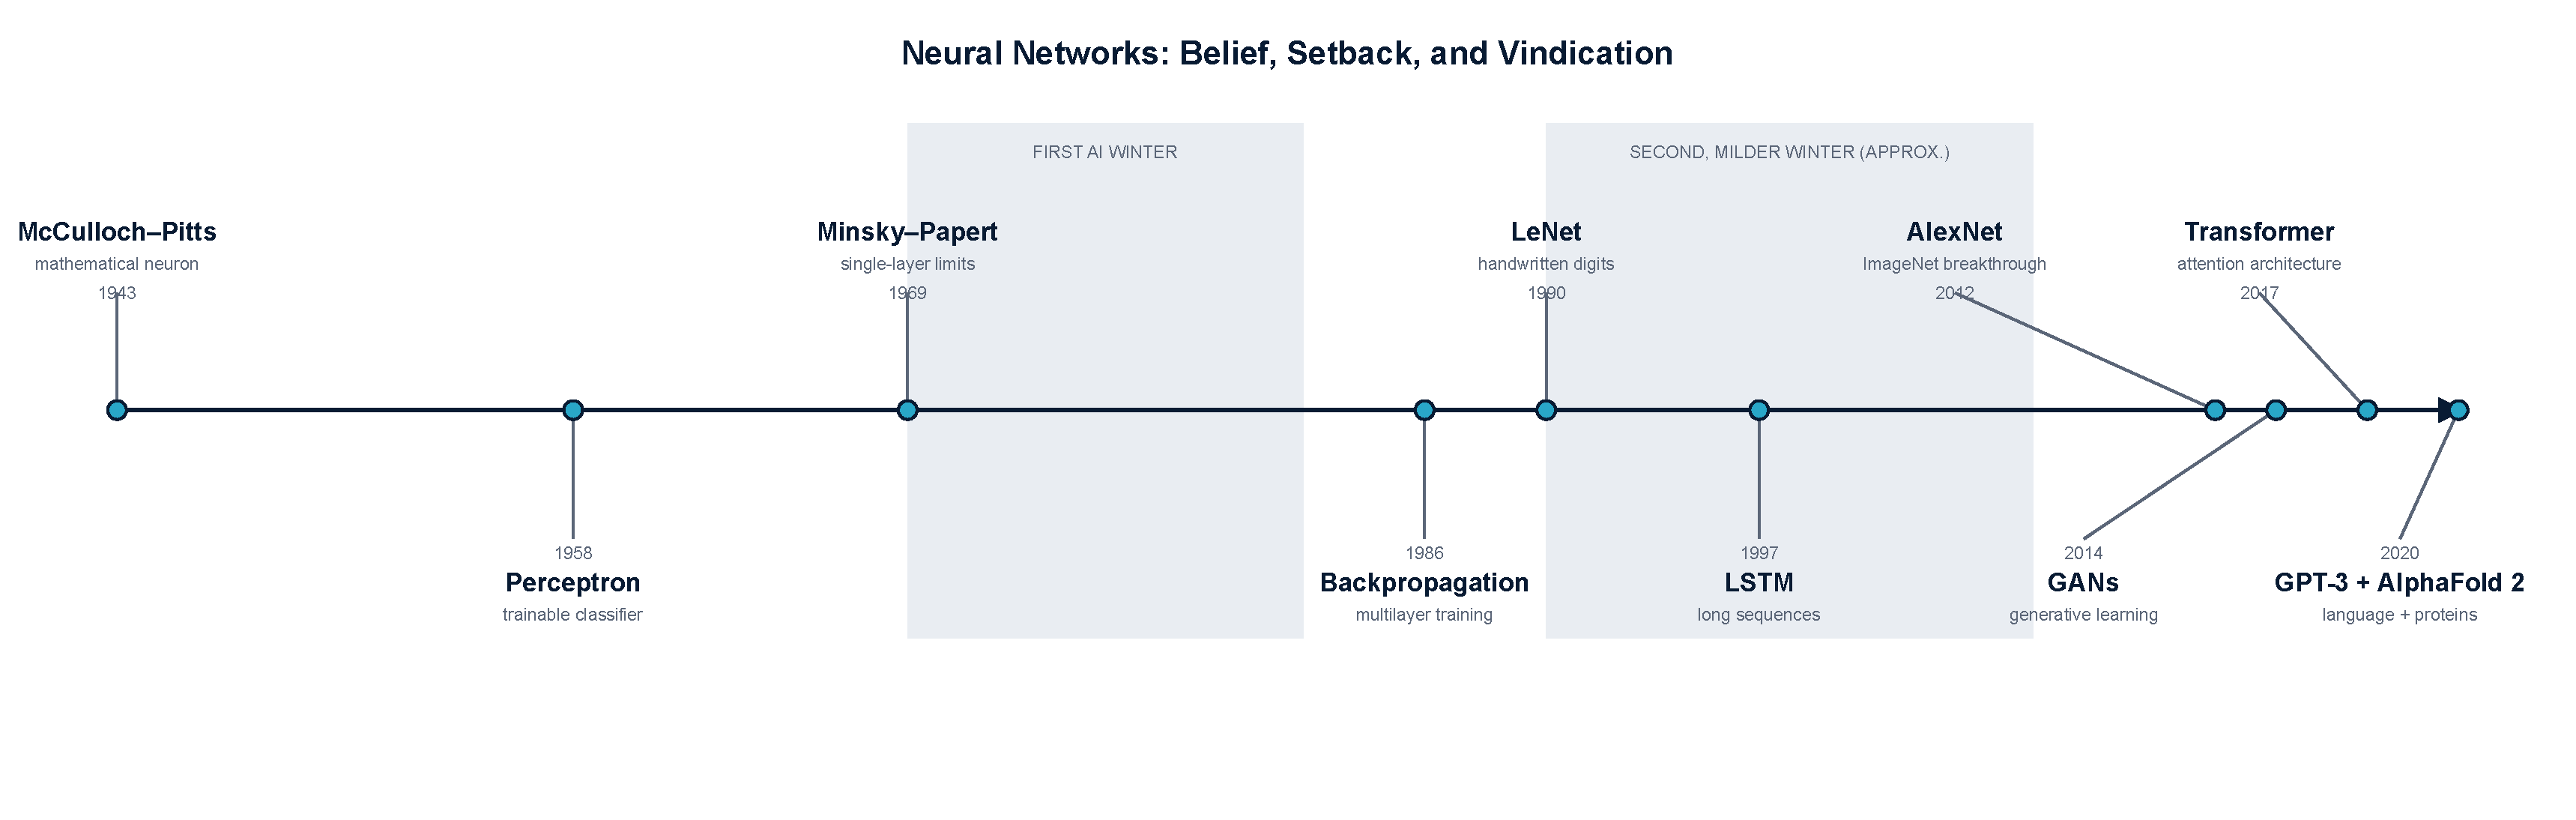
\includegraphics[width=\linewidth,height=.72\textheight,keepaspectratio]{chapters/../assets/figures/fig-1-2-neural-network-timeline.pdf}
\caption*{\emph{Figure 1.2 --- Key milestones in neural network development, from
McCulloch-Pitts (1943) to modern large language models. The two shaded
periods represent the AI Winters. Note that breakthroughs did not stop
during these periods --- they accelerated afterward.}}
\addcontentsline{lof}{figure}{\protect\numberline{1.2}�� Key milestones in neural network development, from McCulloch-Pitts (1943) to modern large language models. The two shaded periods represent the AI Winters. Note that breakthroughs did not stop during these periods — they accelerated afterward.}
\label{figure-1-2}
\end{figure}
\FloatBarrier

\section{The Core Principles: Why Deep Learning
Works}\label{the-core-principles-why-deep-learning-works}

We now have enough context to ask the fundamental question: what
actually makes deep learning powerful? Not the history, not the
applications --- the underlying principles that explain why a layered
neural network can learn to recognize cancer in a scan, translate
between sixty languages, and generate a photorealistic portrait from a
sentence description.

Two principles do most of the explanatory work. They are worth
understanding deeply before we encounter any equations.

\subsection{Principle 1: Hierarchical Feature
Learning}\label{principle-1-hierarchical-feature-learning}

Consider again the task of recognizing a face in a photograph. If you
were to describe this task to a child who had never seen a photograph,
you might say: "Look for two eyes, a nose, a mouth, and two ears,
arranged in roughly this configuration, on a roughly oval surface." The
child learns to recognize faces by learning what faces are made of.

Deep neural networks learn the same way --- except they learn the
components automatically, from scratch, without being told what the
components are. This is hierarchical feature learning, and it is the
most important conceptual innovation in the field.

\subsection{How the Hierarchy Works}\label{how-the-hierarchy-works}

Imagine a deep network processing an image of a dog. At the earliest
layers, the network learns to detect the most primitive visual elements:
edges and gradients --- places where brightness or color changes
sharply. These are not dog-specific features. They appear in images of
everything.

At the next level of layers, the network combines those primitive edges
into something more meaningful: curves, corners, textures, and simple
shapes. Still not specific to dogs --- these features appear in images
of cars and trees and buildings too.

As we move deeper, the combinations become richer and more specific.
Circular shapes combined with certain textures begin to look like eyes.
Curved edges in certain configurations begin to look like snouts. By the
time we reach the deepest layers --- what some researchers call the
"executive" layers --- the network has assembled rich, complex
representations: "this combination of features is consistent with a
dog\textquotesingle s face."

The crucial insight is that none of these features were specified by a
human. No programmer told the network to look for edges, or curves, or
snouts. The network discovered these features because they were
statistically useful for distinguishing dogs from everything else in the
training data. The features are the network\textquotesingle s own
invention.

\begin{figure}[htbp]
\centering
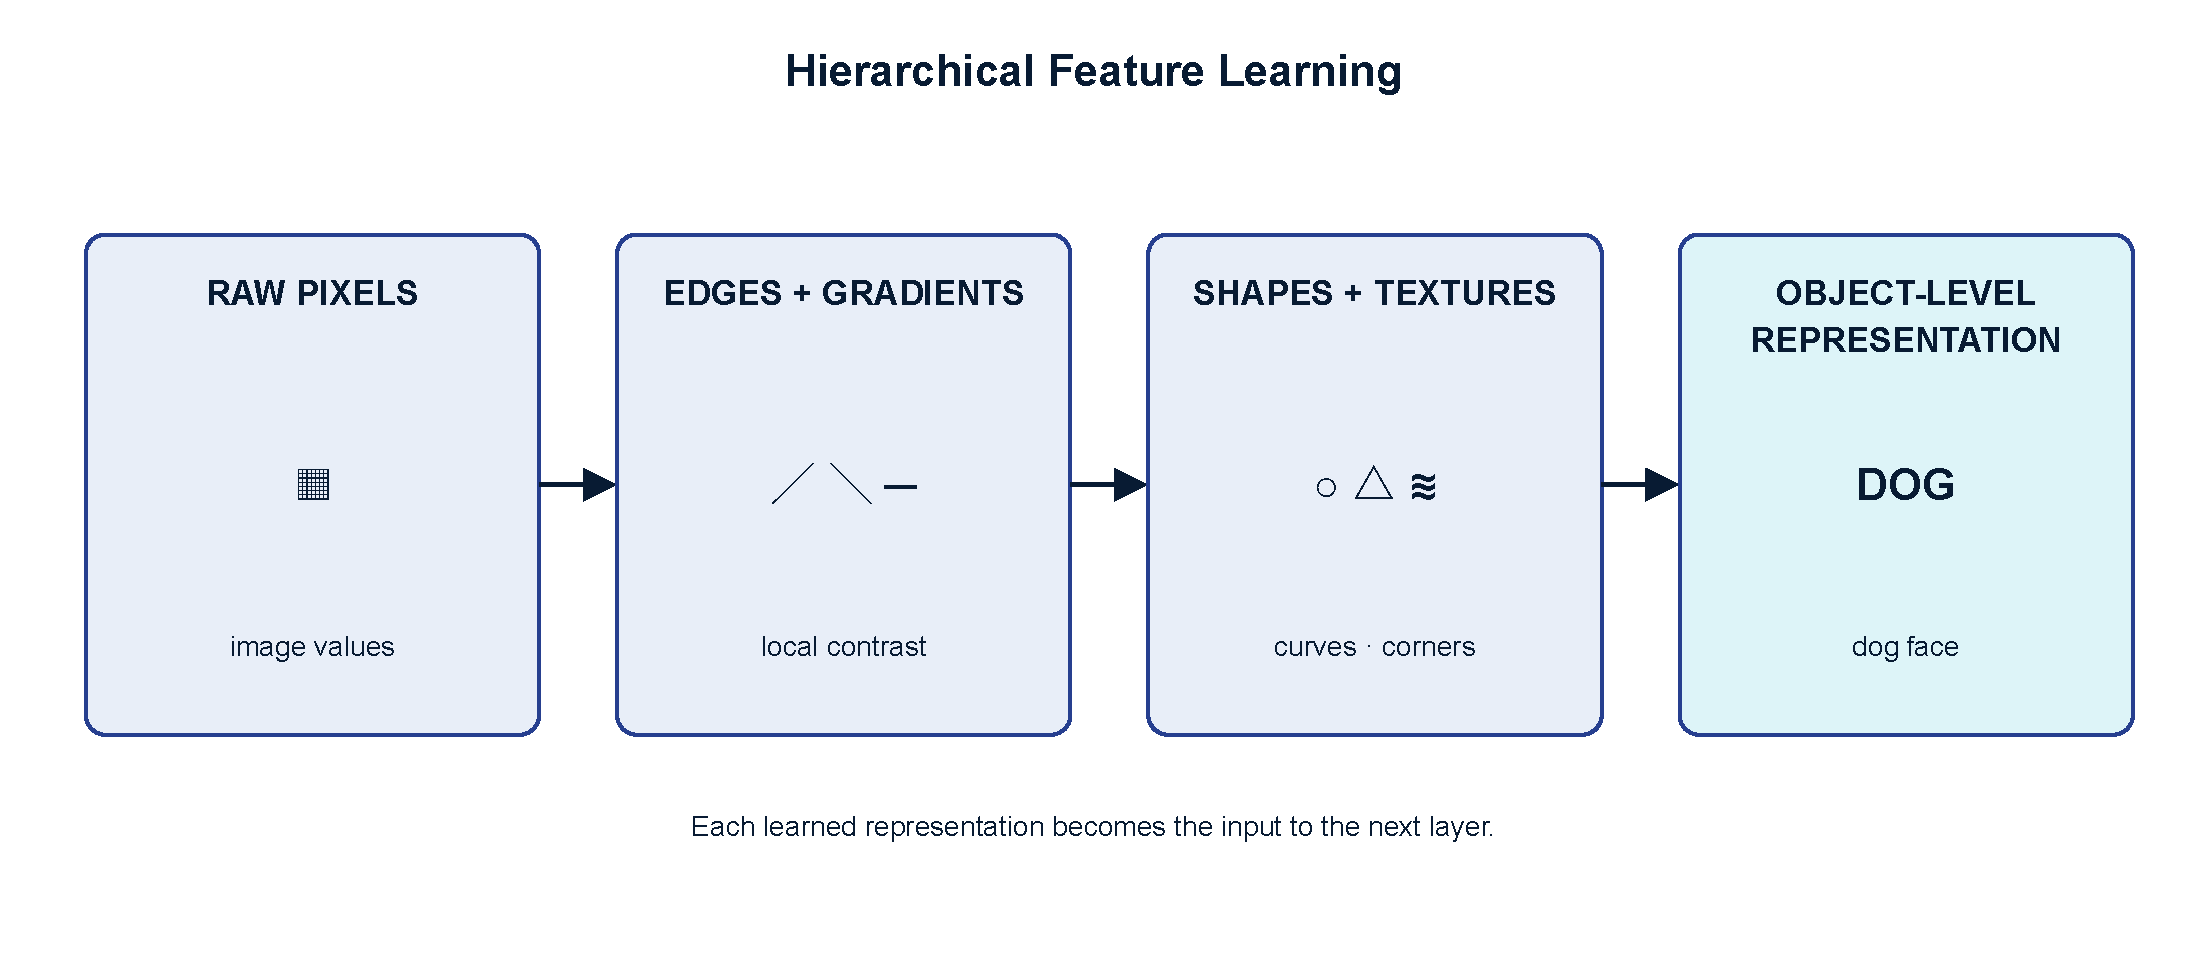
\includegraphics[width=\linewidth,height=.72\textheight,keepaspectratio]{chapters/../assets/figures/fig-1-3-hierarchical-feature-learning.pdf}
\caption*{\emph{Figure 1.3 --- Hierarchical feature learning in a convolutional
network. The same image passes through four progressive layers: raw
pixels, edge detection, shape assembly, and object recognition. Each
layer builds on the representations learned by the layer before it.}}
\addcontentsline{lof}{figure}{\protect\numberline{1.3}�� Hierarchical feature learning in a convolutional network. The same image passes through four progressive layers: raw pixels, edge detection, shape assembly, and object recognition. Each layer builds on the representations learned by the layer before it.}
\label{figure-1-3}
\end{figure}
\FloatBarrier

\subsection{Why This Is Revolutionary}\label{why-this-is-revolutionary}

Before deep learning, building a vision system meant feature
engineering: a domain expert would spend months or years designing the
features --- deciding what to measure, what to extract, what to feed
into the classifier. The performance of the system was fundamentally
bounded by the quality of the human-designed features. If the expert
missed something important, the system missed it too.

Feature learning eliminates this bottleneck. The network discovers
features that no human designer thought to specify --- features that, in
many cases, turn out to be more predictive than any human-designed
alternative. This is not a small optimization. It is a qualitative
change in what kinds of problems can be addressed.

It also explains a pattern we will see throughout this course: deep
learning tends to outperform traditional approaches most decisively on
problems involving rich, unstructured data --- images, audio, natural
language --- precisely because these are the domains where manual
feature engineering is hardest.

\subsection{Principle 2: Representation
Learning}\label{principle-2-representation-learning}

Hierarchical feature learning explains how deep networks process raw
data. Representation learning explains what they produce: a deep network
does not just make a prediction about its input --- it builds a rich
internal model of the world it has been trained on.

\subsection{The Concept of an
Embedding}\label{the-concept-of-an-embedding}

Here is an experiment that illuminates the idea. Take a state-of-the-art
image network and remove the final classification layer. What remains is
a function that maps any image to a long list of numbers --- typically
512 or 2,048 numbers. This list is called an embedding, or a
representation.

Now take two photographs of the same dog, taken from different angles on
different days. Feed both through the network. Their embeddings will be
remarkably similar --- not identical, but close. Now take a photograph
of a cat and feed it through. Its embedding will be noticeably different
from both dog photographs, but will cluster with other cat embeddings.

The network has learned a secret language for images. In this language,
similarity of meaning corresponds to similarity in the numerical
representation. Two images that depict similar things will be encoded
similarly, even if they look nothing alike at the pixel level.

This is a profound capability. It means the network has done something
more than classify --- it has learned to understand, in a functional
sense, the relationships between the things it has seen.

\subsection{Why Representations
Matter}\label{why-representations-matter}

The practical implications are substantial. Once a network has learned a
good representation of images, that representation can be reused for
tasks the network was never explicitly trained for. A network trained to
recognize 1,000 categories of everyday objects has built representations
that are useful for detecting diseases in medical images, for searching
satellite imagery, for identifying plant species, and for dozens of
other tasks --- even though its training data contained none of these
things.

This is the foundation of transfer learning, one of the most practically
important ideas in the field. Rather than training a new network from
scratch for every problem --- which requires enormous data and compute
--- practitioners can start with a network that already has good
representations and fine-tune it for their specific task. The effort
required drops from months and millions of dollars to days and thousands
of dollars.

\begin{quote}
\emph{A network trained on one thing has learned something more general
than that thing. Representations are the portable, reusable knowledge of
deep learning.}
\end{quote}

\subsection{Representation Learning and the Curse of
Dimensionality}\label{representation-learning-and-the-curse-of-dimensionality}

There is a deeper reason why representation learning matters, connected
to a fundamental challenge in all of machine learning: the curse of
dimensionality. Raw data --- images, audio, text --- exists in extremely
high-dimensional spaces. A modest 224×224 color image has 150,528
dimensions. Finding patterns in spaces this large requires either
enormous amounts of data or a way to focus attention on the structure
that matters.

Deep networks address this challenge by learning compact,
low-dimensional representations that capture the essence of the data.
The 150,528 dimensions of a photograph can be distilled into 512
meaningful numbers that capture everything the network needs to know
about what the image depicts. This compression is not lossy in any
harmful sense --- it discards the irrelevant variation (lighting
conditions, camera angle, background clutter) while preserving the
signal (what is depicted and how it relates to other things in the
world).

\subsection{What Emerges from These Two
Principles}\label{what-emerges-from-these-two-principles}

When hierarchical feature learning and representation learning work
together in a deep network trained on sufficient data, something
remarkable emerges: capabilities that were not explicitly programmed and
were not straightforwardly predictable from the training objective.

Networks trained to classify images learn to detect the style of
individual artists, even though no one labeled the training images by
artistic style. Language models trained to predict the next word develop
internal representations of grammar, syntax, and factual relationships
--- without ever being taught these concepts explicitly. Networks
trained on protein sequences develop representations that capture the
physical chemistry of amino acid interactions.

These emergent capabilities are not magic. They are the consequence of
building representations rich enough to support the training task, which
turn out to be rich enough to support much more. Understanding when and
why this emergence happens --- and when it fails to happen --- is one of
the active frontiers of deep learning research.

\section{Deep Learning vs.~Traditional Machine Learning: Choosing the
Right
Tool}\label{deep-learning-vs.-traditional-machine-learning-choosing-the-right-tool}

Having spent time inside deep learning, it is worth stepping back to
ask: when should you not use it? Deep learning is powerful, but it is
not universally appropriate. Understanding its relationship to
traditional machine learning --- and the conditions under which each
approach is superior --- is one of the most practically important skills
in the field.

We will compare the two approaches along six dimensions. Rather than
treating this as a competition, think of it as a map: different
territories call for different tools, and the best practitioners know
which territory they are in.

\subsection{1. Feature Extraction: Designed
vs.~Discovered}\label{feature-extraction-designed-vs.-discovered}

Traditional machine learning requires a human expert to design the
features --- the aspects of the raw data that will be fed to the
learning algorithm. A credit scoring model might be fed income,
debt-to-income ratio, employment duration, and credit history --- all
carefully chosen by a financial domain expert. The
model\textquotesingle s job is to combine these features effectively,
but the feature choices themselves are human decisions.

The strength of this approach is that it incorporates domain knowledge
directly. The weakness is that it is bounded by that knowledge: if the
expert misses something important, the model cannot discover it. It also
requires substantial expert time and becomes increasingly impractical as
the raw data becomes more complex --- nobody can hand-engineer useful
features for a 224×224 color image.

Deep learning discovers its own features. This eliminates the bottleneck
of expert time and allows the model to find patterns that human
designers would never have thought to look for. The cost is that the
discovered features are often uninterpretable --- we know they work, but
we cannot always explain what they represent.

\subsection{2. Data Types: Structured
vs.~Unstructured}\label{data-types-structured-vs.-unstructured}

Traditional machine learning methods were developed primarily for
structured data: tabular data with well-defined rows and columns, where
each column represents a specific, measurable attribute. A spreadsheet
of house prices with columns for square footage, number of bedrooms, and
neighborhood is the natural habitat of traditional ML. Given such data,
methods like gradient boosting and random forests remain highly
competitive --- often superior to deep learning.

Deep learning\textquotesingle s advantage emerges with unstructured
data: images, audio, natural language, video, and sequences of events.
These data types do not fit naturally into tables. Their meaningful
patterns require hierarchical feature extraction --- exactly the
capability deep networks provide. This is why the domains where deep
learning has had the largest impact --- computer vision, speech
recognition, natural language processing --- are all unstructured data
domains.

\subsection{3. Scalability: Ceilings vs.~Scaling
Laws}\label{scalability-ceilings-vs.-scaling-laws}

Traditional machine learning methods tend to improve rapidly with
relatively small amounts of data, then plateau. Adding more training
examples beyond a certain point produces diminishing returns. This is
not a criticism --- it reflects the fact that these methods are making
efficient use of what they have, and there is simply a limit to what can
be learned from the features they are given.

Deep learning exhibits a different relationship with data: scaling laws.
With more data, larger models, and more compute, performance continues
to improve --- often without any clear ceiling. This was first
demonstrated dramatically with AlexNet and has been confirmed across
domains. The largest language models trained on trillions of tokens
outperform smaller models trained on the same data by substantial
margins.

This scaling behavior is both a strength and a practical constraint. It
means deep learning rewards investment: organizations with more data,
more compute, and larger models will build better systems. It also means
that deep learning can be overkill for problems where the available data
is small or the performance ceiling of traditional methods is already
sufficient.

\subsection{4. Interpretability: Glass Boxes and Black
Boxes}\label{interpretability-glass-boxes-and-black-boxes}

A decision tree, the simplest family of traditional ML models, is almost
completely interpretable. You can follow every branch from root to leaf
and reconstruct exactly why the model made a given prediction: "This
loan application was rejected because the applicant\textquotesingle s
debt-to-income ratio exceeds 0.43 and their employment duration is less
than two years." This kind of explanation is valuable in regulated
industries where decisions affecting people\textquotesingle s lives must
be justifiable.

Deep neural networks, especially deep ones with hundreds of millions of
parameters, are not interpretable in this direct sense. The mapping from
input to output passes through many layers of nonlinear transformation,
and no single weight or layer encodes a human-understandable decision
rule. When a deep network classifies a tumor as malignant, it cannot
produce a concise explanation of why. This is the "black box" problem,
and it is real.

It is also not static. A growing subfield called explainable AI (XAI)
develops tools for peering inside deep networks --- identifying which
parts of an input the network attended to, which training examples
influenced a given prediction, and which features the network has
implicitly learned to use. These tools do not turn deep networks into
glass boxes, but they reduce the opacity meaningfully. We will examine
them later in the course.

The practical implication: in domains where interpretability is legally
required --- certain financial decisions, medical diagnoses where the
rationale must be documented --- the interpretability of traditional
methods may be decisive, independent of the accuracy advantage deep
learning offers.

\subsection{5. Computational Resources: Laptops and Data
Centers}\label{computational-resources-laptops-and-data-centers}

A random forest or gradient boosting model can be trained in minutes on
a laptop. A simple deep learning model for image classification can be
trained in hours on a consumer GPU. A state-of-the-art language model
requires months on thousands of specialized GPUs, at a cost of millions
of dollars and a substantial carbon footprint.

This range is important to internalize. Not every deep learning problem
requires frontier resources, and not every problem that can be tackled
with deep learning should be. The most responsible engineering practice
involves choosing the least resource-intensive approach that is
sufficient for the task --- a principle that is both economically and
environmentally sound.

\subsection{6. Data Requirements: Snacks and
Feasts}\label{data-requirements-snacks-and-feasts}

Traditional machine learning methods can produce useful models from
hundreds or thousands of examples. This makes them indispensable in
domains where labeled data is scarce, expensive to collect, or limited
by the rarity of the phenomenon being modeled. A rare disease diagnosis
model may have access to only a few hundred confirmed cases --- a feast
for traditional methods, a famine for deep learning.

Deep learning typically requires thousands to millions of labeled
examples to reach its potential. This appetite is why the field exploded
when ImageNet became available (1.2 million labeled images), and why
large language models are trained on essentially the entire internet.
When data is abundant, deep learning thrives. When it is scarce,
traditional methods or transfer learning are often the better choice.

\begin{longtable}[]{@{}
  >{\raggedright\arraybackslash}p{(\linewidth - 4\tabcolsep) * \real{0.1984}}
  >{\raggedright\arraybackslash}p{(\linewidth - 4\tabcolsep) * \real{0.3889}}
  >{\raggedright\arraybackslash}p{(\linewidth - 4\tabcolsep) * \real{0.3968}}@{}}
\toprule\noalign{}
\begin{minipage}[b]{\linewidth}\raggedright
\textbf{Dimension}
\end{minipage} & \begin{minipage}[b]{\linewidth}\raggedright
\textbf{Traditional Machine Learning}
\end{minipage} & \begin{minipage}[b]{\linewidth}\raggedright
\textbf{Deep Learning}
\end{minipage} \\
\midrule\noalign{}
\endhead
\bottomrule\noalign{}
\endlastfoot
Feature extraction & Human-designed; requires domain expertise &
Automatic; discovered from raw data \\
Best data types & Structured, tabular data & Unstructured: images, text,
audio, video \\
Performance with scale & Plateaus with more data & Continues improving
with more data and compute \\
Interpretability & Often transparent; decisions can be explained & Often
opaque; "black box" behavior \\
Compute requirements & Modest; trainable on a laptop & Substantial;
often requires GPUs or TPUs \\
Data requirements & Hundreds to thousands of examples & Thousands to
millions of examples \\
Development speed & Fast iteration cycles & Longer training and
experimentation cycles \\
Best use cases & Tabular data, regulated industries, small data &
Complex perception, generation, large-scale NLP \\
\end{longtable}

The wisest practitioners are not loyal to either camp. They understand
the terrain of the problem in front of them --- the data type, the
quantity, the interpretability requirements, the compute budget, the
performance target --- and choose accordingly. Many of the best systems
in production today are hybrids: deep learning for the perception or
representation step, traditional methods for the final decision layer
where interpretability matters.

\section{Introducing the Capstone Project:
MIPDS}\label{introducing-the-capstone-project-mipds}

Throughout this course, you will build something. Not a series of
isolated exercises, but a single evolving system that grows in
capability each week as you add what you have learned. By the final
week, you will have a functioning Multimodal Intelligent Perception and
Decision System --- MIPDS.

\subsection{What MIPDS Will Do}\label{what-mipds-will-do}

At full capability, MIPDS will be able to perceive and understand
images, using convolutional neural networks and vision transformers to
extract meaning from visual input. It will understand language, using
transformer-based language models to process text. It will reason across
modalities --- connecting what it sees to what it reads. It will
generate output, using generative models to produce images, text, or
descriptions. And it will make decisions, using reinforcement learning
to act in the world based on its perceptions.

No single week will build all of this. Each chapter adds one capability
--- a new component, a new module, a new layer of intelligence. By the
time you finish, you will not just have read about deep
learning\textquotesingle s capabilities. You will have built them.

\subsection{This Week: The Blueprint}\label{this-week-the-blueprint}

Before writing a line of code, we need to think. The most important
decisions in any complex system are made at the design philosophy level
--- decisions about purpose, about scope, about who benefits and who
might be harmed.

Your task this week is to write a one-page MIPDS Design Philosophy
Document. It should address four questions:

\begin{enumerate}
\def\labelenumi{\arabic{enumi}.}
\setcounter{enumi}{8}
\item
  Purpose: What problem should MIPDS solve? What kind of perception and
  decision-making should it enable?
\item
  Capabilities: What should it be able to see, understand, generate, and
  decide? Be aspirational --- we will constrain later.
\item
  Stakeholders: Who might use such a system? Who else might be affected
  by it, with or without their knowledge?
\item
  Risks: What could go wrong before you build a single component? What
  harms could this system enable?
\end{enumerate}

This document will be a living artifact. You will update it every week
as your technical understanding grows and your design decisions become
more informed. By Week 16, it will be both a design record and a
reflection on how understanding changes what you build.

\subsection{Setting Up Your Development
Environment}\label{setting-up-your-development-environment}

While your conceptual thinking develops, you will also set up the
infrastructure for everything that follows. A working deep learning
environment is the foundation for all the hands-on work ahead.

\subsection{Step 1: Python
Installation}\label{step-1-python-installation}

Download Python 3.10 or later from python.org. During installation,
ensure that Python is added to your system PATH. A clean installation
into a dedicated project directory --- rather than modifying your system
Python --- will prevent the dependency conflicts that are the most
common source of frustration for new practitioners.

\subsection{Step 2: Virtual
Environment}\label{step-2-virtual-environment}

Every serious Python project should live in its own virtual environment
--- an isolated container that holds its dependencies separately from
every other project. Create and activate your environment with:

python -m venv mipds\_env

source mipds\_env/bin/activate \# macOS/Linux

mipds\_env\textbackslash Scripts\textbackslash activate \# Windows

\subsection{Step 3: Core Dependencies}\label{step-3-core-dependencies}

Install the libraries you will use throughout the course:

pip install tensorflow numpy matplotlib pillow jupyter scikit-learn

If you have a CUDA-capable GPU and want to use it (highly recommended
for any serious training), follow the GPU setup guide in the course
companion materials, which provides version-matched instructions for
your hardware and operating system.

\subsection{Step 4: Verifying Your
Setup}\label{step-4-verifying-your-setup}

Run the provided verification notebook (setup\_check.ipynb) from the
course repository. This notebook checks that all dependencies are
installed correctly, confirms whether a GPU is available, and loads a
pre-trained model to confirm that the full inference pipeline works.
Completing this verification before the first hands-on assignment will
save significant time later.

\subsection{Step 5: Version Control}\label{step-5-version-control}

Initialize a git repository in your project directory and create a
remote repository on GitHub or GitLab. Every piece of work you produce
this semester --- code, design documents, experiment logs --- should
live in this repository. Version control is not optional for serious
practitioners; it is the foundation of reproducible research.

\addcontentsline{toc}{section}{Hands-On Exploration}
\begin{DLSectionPanel}{HANDS-ON EXPLORATION}

\subsection{Feature Engineering vs.~Feature
Learning}\label{feature-engineering-vs.-feature-learning}

\subsection{The Activity}\label{the-activity}

Before writing a neural network, let us build intuition for why the
feature learning approach matters. This exploration requires no deep
learning knowledge --- only curiosity and a willingness to observe
carefully.

Open the notebook hands\_on\_ch1.ipynb from the course repository. It
contains a dataset of 200 hand-drawn shapes (circles, squares, and
triangles) with their labels.

\subsection{Part 1: Write Your Own Rules (15
minutes)}\label{part-1-write-your-own-rules-15-minutes}

Before running any model, look at a sample of the shapes. Then write ---
in plain English --- three rules that you think would correctly classify
any shape as a circle, square, or triangle. For example: "If the object
has straight edges and four corners of equal length, it is a square."

The notebook includes a cell that converts your verbal rules into a
simple rule-based classifier. Run it on the test set and record the
accuracy.

\subsection{Part 2: When Rules Break (10
minutes)}\label{part-2-when-rules-break-10-minutes}

A second test set contains the same shapes --- but rotated, partially
obscured, drawn in different sizes, and in some cases drawn by a
different person. Run your rule-based classifier on this second set.
What changes? What breaks? Document your observations carefully.

\subsection{Part 3: Feature Learning in Action (10
minutes)}\label{part-3-feature-learning-in-action-10-minutes}

A pre-trained three-layer convolutional network is provided in the
notebook. Run it on both test sets and compare its accuracy to your
rule-based classifier. Then run the provided visualization cell, which
shows you the patterns the network\textquotesingle s first layer has
learned to detect --- the features it discovered without being told what
to look for.

\subsection{Reflection Questions}\label{reflection-questions}

Write a 200- to 300-word reflection in the notebook addressing the
following:

\begin{enumerate}
\def\labelenumi{\arabic{enumi}.}
\setcounter{enumi}{12}
\item
  What rules did you write in Part 1? Were they complete? What cases did
  they miss?
\item
  What happened to your rules in Part 2? What does this tell you about
  the brittleness of manually designed features?
\item
  What did the first-layer visualizations look like? Did the network
  learn what you expected? Did anything surprise you?
\item
  Where do you think rule-based approaches still have advantages over
  learned features?
\end{enumerate}

\end{DLSectionPanel}

\section{Case Study}\label{case-study}

\subsection{AlexNet (2012): The Moment That Changed
Everything}\label{alexnet-2012-the-moment-that-changed-everything}

\subsection{The Problem}\label{the-problem}

The ImageNet Large Scale Visual Recognition Challenge, known as ILSVRC,
was an annual competition that asked teams to build systems capable of
classifying images from a dataset of 1.2 million photographs into 1,000
categories --- from "goldfinch" to "volcano" to "espresso." The
challenge was designed to push the state of the art in computer vision,
and for three years it had done exactly that --- but incrementally. The
best systems in 2010 and 2011 used hand-engineered visual features
combined with traditional classifiers. The top-5 error rate --- the
fraction of images for which the correct label was not among the
system\textquotesingle s five guesses --- was hovering around 26
percent.

\subsection{The Deep Learning
Solution}\label{the-deep-learning-solution}

In 2012, a team from the University of Toronto entered with AlexNet: a
deep convolutional neural network with eight layers, sixty million
parameters, and a design that incorporated several innovations that
together proved decisive. The network was trained on two NVIDIA GTX 580
graphics processing units over six days. Its top-5 error rate was 15.3
percent --- nearly eleven percentage points better than the previous
year\textquotesingle s winner.

To put that margin in context: the difference between first and second
place in the previous two competitions had been less than one percentage
point. AlexNet did not just beat the competition --- it invalidated the
previous era\textquotesingle s approach.

\subsection{Why Deep Learning Was the Right
Tool}\label{why-deep-learning-was-the-right-tool}

AlexNet succeeded because the structure of the problem matched the
strengths of convolutional networks. Raw image data contains patterns
that are spatially local (an edge detector does not need to look at the
whole image), hierarchical (edges compose into shapes, shapes compose
into objects), and translation-invariant (a dog is a dog regardless of
where in the frame it appears). Convolutional networks encode all three
of these properties into their architecture. No amount of feature
engineering could replicate the flexibility of a system that discovers
its own features end-to-end.

Three specific innovations in AlexNet contributed to its margin. The
ReLU activation function, which simply passes positive values and zeros
out negative ones, trained much faster than the sigmoid functions used
in earlier work without sacrificing accuracy. Dropout regularization,
which randomly deactivated half the neurons during training,
dramatically reduced overfitting on a scale that would otherwise have
been devastating. And data augmentation --- artificially generating
additional training examples by cropping, flipping, and adjusting the
color of existing images --- expanded the effective training set by
orders of magnitude.

\subsection{Tradeoffs and Limitations}\label{tradeoffs-and-limitations}

AlexNet was not without limitations, and understanding them is as
important as understanding its successes. Training required specialized
hardware that was unavailable to most researchers in 2012 --- the two
gaming GPUs cost more than a thousand dollars at the time, and the
electricity and cooling costs were non-trivial. The training process
took six days; modern practitioners with better hardware and better
optimization algorithms can achieve comparable results in hours, but the
resource barrier was real.

More fundamentally, AlexNet was a black box. It could identify a
goldfinch in a photograph with remarkable accuracy, but it could not
explain what it was looking at that told it "goldfinch." Subsequent work
showed that it was, in some cases, using spurious features ---
classifying images partly based on background context rather than the
object itself. A husky photographed in the snow might be correctly
identified partly because of the snow, not because of the dog. This
brittleness to distribution shift --- to encountering inputs that look
superficially different from the training data --- would prove to be a
persistent challenge across the field.

AlexNet was also shown to be vulnerable to adversarial examples:
carefully crafted pixel perturbations, invisible to the human eye, that
caused the network to misclassify images with high confidence. A panda
that a human would never mistake for anything else becomes, for AlexNet,
a gibbon after a few carefully chosen pixel adjustments. This discovery,
made by Szegedy and colleagues in 2013, opened a line of research in
adversarial machine learning that continues to this day and has
significant implications for the security of any system that relies on
deep learning classifiers.

\subsection{The Broader Lesson}\label{the-broader-lesson}

AlexNet\textquotesingle s legacy is not primarily architectural. The
specific network design has long since been superseded by deeper, wider,
and more efficient successors. Its legacy is the demonstration of a
principle: that with the right architecture, sufficient data, and
sufficient compute, deep learning would outperform any other approach on
problems involving rich, unstructured perceptual data --- and would
continue to improve as those three ingredients scaled. This insight,
confirmed and extended year after year, drove the investment in data
collection, compute infrastructure, and research talent that produced
the AI landscape we inhabit today.

\addcontentsline{toc}{section}{Chapter Summary}
\begin{DLSectionPanel}{CHAPTER SUMMARY}

\subsection{What We Have Learned}\label{what-we-have-learned}

We began this chapter with a chest X-ray and a question about a
fundamentally different way of building intelligent systems. We end it
with the conceptual foundations needed to understand the answer.

Deep learning is a specific approach within machine learning: the use of
neural networks with many layers to learn hierarchical representations
of data from examples. It sits within the broader circle of machine
learning, which sits within the broader circle of artificial
intelligence --- each level more capable and more demanding than the
last.

The history of neural networks is a story of persistence. The field was
born in the 1940s, flourished briefly in the late 1950s, was nearly
killed by a mathematical critique in 1969, survived in the margins
through the 1970s and early 1980s, was revived by backpropagation in the
mid-1980s, and spent two more decades as a technically capable but
commercially marginal approach. AlexNet\textquotesingle s decisive
victory in 2012 ended that era and began the one we are living in.

Two principles explain deep learning\textquotesingle s power.
Hierarchical feature learning allows networks to automatically discover
the features that distinguish one class of input from another --- from
edges and textures to object parts to complete semantic categories ---
without being told what to look for. Representation learning allows
networks to build rich internal models of the world they have been
trained on --- models whose structure captures the semantic
relationships between things, and whose compact form supports transfer
to new tasks.

Deep learning is not always the right tool. Traditional machine learning
methods outperform it on structured tabular data, in low-data regimes,
in contexts where interpretability is legally required, and when
computational resources are constrained. The skill is not knowing how to
build deep networks --- it is knowing when to build them.

You have also taken the first step toward your semester-long capstone
project: the MIPDS Design Philosophy Document. What begins this week as
a statement of aspiration will, over sixteen weeks, become a technical
design document reflecting everything you have learned. The system will
grow. So will your understanding of what it means to build something
intelligent --- and what it means to build it responsibly.

In Chapter 2, we will open the hood of the neural network. We will
discover that the magic of hierarchical learning reduces, at its
foundation, to a specific computation: weighted sums followed by
nonlinear functions, repeated across millions of connections and
billions of training steps. The math is not complicated. The
consequences are extraordinary.

\end{DLSectionPanel}

\addcontentsline{toc}{section}{Review Questions}
\begin{DLSectionPanel}{REVIEW QUESTIONS}

\subsection{Questions for Reflection and
Debate}\label{questions-for-reflection-and-debate}

These questions have no single correct answers. They are designed to be
debated, refined, and revisited as your understanding deepens throughout
the course.

\subsection{1. The Explanation Problem}\label{the-explanation-problem}

A deep learning system correctly identifies early-stage pancreatic
cancer in a scan with 94 percent accuracy --- significantly better than
the 78 percent accuracy of an experienced radiologist. But the system
cannot explain which features in the scan led to its classification.
Should a physician use it to guide treatment decisions? What would it
take for you to trust an unexplained prediction in a high-stakes medical
context?

\subsection{2. The Two Winters and Scientific
Progress}\label{the-two-winters-and-scientific-progress}

Neural network research survived two periods of widespread skepticism
and funding withdrawal because a small community kept working despite
the dismissal of the broader field. What does this tell us about how
scientific progress actually happens? Are there ideas being dismissed
today that will be vindicated in ten years? How would you evaluate them?

\subsection{3. The Resource Divide}\label{the-resource-divide}

Training a state-of-the-art large language model costs tens of millions
of dollars and consumes electricity comparable to that of a small town
for several months. This means only the largest technology companies and
best-funded research institutions can push the frontier of capability.
What are the implications of this concentration for academic research?
For international AI development? For the diversity of perspectives
embedded in frontier AI systems?

\subsection{4. Feature Engineering as Domain
Knowledge}\label{feature-engineering-as-domain-knowledge}

When a human expert designs features for a machine learning model, they
are embedding their understanding of the domain into the system. When a
deep network learns features automatically, that knowledge is implicit
and often uninterpretable. Which approach produces more trustworthy
systems? Is trust the right criterion --- or should we prioritize
accuracy, or fairness, or something else?

\subsection{5. Training Data and
Consent}\label{training-data-and-consent}

Large language models and image generation systems are trained on text
and images scraped from the internet --- including works created by
millions of writers, artists, photographers, and musicians who did not
consent to their use as training data. What ethical framework should
govern this practice? Does the social benefit of capable AI systems
justify the use of unconsented training data? Who should decide?

\subsection{6. The Responsibility Gap}\label{the-responsibility-gap}

A deep learning system is trained on data from 2020, deployed in 2022,
and used in a clinical setting in 2024. The patient population has
shifted. The imaging equipment has been upgraded. The demographics of
the patients being scanned have changed. The system\textquotesingle s
accuracy has quietly degraded. Who is responsible for detecting and
addressing this drift: the developers who trained it, the hospital that
deployed it, the regulatory agency that approved it, or the clinicians
who rely on it?

\subsection{7. AI Winters and the
Present}\label{ai-winters-and-the-present}

Given the history of AI Winters, how would you distinguish between
genuine transformative capability and a technology bubble in the current
AI landscape? What evidence would convince you that the current wave of
deep learning progress has hit a ceiling? What evidence would convince
you it has not?

\subsection{8. Choosing Your Adventure}\label{choosing-your-adventure}

Think of a problem in your own field, area of interest, or daily life
that might benefit from machine learning. Work through the
six-dimensional comparison from Section 4. Is deep learning likely to be
the right approach? What additional information would you need to answer
that question with confidence?

\end{DLSectionPanel}

\addcontentsline{toc}{section}{Further Reading}
\begin{DLSectionPanel}{FURTHER READING}

\subsection{Going Deeper}\label{going-deeper}

The following resources are organized by theme. Start with whichever
thread interests you most.

\subsection{On the History and Culture of Deep
Learning}\label{on-the-history-and-culture-of-deep-learning}

Goodfellow, I., Bengio, Y., \& Courville, A. (2016). Deep Learning. MIT
Press. The standard reference text; Chapter 1 provides an authoritative
historical account. Available free online at deeplearningbook.org.

Marcus, G., \& Davis, E. (2019). Rebooting AI: Building Artificial
Intelligence We Can Trust. Pantheon Books. A critical and highly
readable perspective on the limits of current deep learning, useful for
calibrating optimism.

Metz, C. (2021). Genius Makers: The Mavericks Who Brought AI to Google,
Facebook, and the World. Dutton. Narrative journalism that tells the
human story of the deep learning revolution.

\subsection{On Foundations and
Principles}\label{on-foundations-and-principles}

LeCun, Y., Bengio, Y., \& Hinton, G. (2015). Deep learning. Nature,
521(7553), 436--444. The landmark review article by three of the
field\textquotesingle s founders. Accessible to a general scientific
audience.

Schmidhuber, J. (2015). Deep learning in neural networks: An overview.
Neural Networks, 61, 85--117. A comprehensive historical account with
broader coverage than most introductory treatments.

\subsection{On Ethics and Society}\label{on-ethics-and-society}

O\textquotesingle Neil, C. (2016). Weapons of Math Destruction: How Big
Data Increases Inequality and Threatens Democracy. Crown. Essential
context for understanding how algorithmic systems can cause harm at
scale.

Gebru, T., Morgenstern, J., Vecchione, B., Vaughan, J. W., Daumé III,
H., Iii, H. D., \& Crawford, K. (2018). Datasheets for Datasets.
arXiv:1803.09010. A foundational paper proposing standards for
documenting training data --- directly relevant to the consent issues
raised in this chapter.

\subsection{On Applications}\label{on-applications}

Rajpurkar, P., Irvin, J., Ball, R. L., et al.~(2017). CheXNet:
Radiologist-Level Pneumonia Detection on Chest X-Rays with Deep
Learning. arXiv:1711.05225. The paper behind the CheXNet system
discussed in this chapter\textquotesingle s opening narrative.

Senior, A. W., Evans, R., Jumper, J., et al.~(2020). Improved protein
structure prediction using potentials from deep learning. Nature,
577(7792), 706--710. The AlphaFold work that transformed structural
biology.

\emph{--- End of Chapter 1 ---}

\end{DLSectionPanel}

\DLChapterOpener{Foundations of Deep Learning}{Neural Network Architectures}{The Blueprint of Artificial Minds}{\item \textbf{Explain the biological inspiration} behind artificial neural
networks, and articulate clearly where the analogy between brains and
machines breaks down.
\item \textbf{Describe the structural components} of any neural network ---
input layers, hidden layers, output layers, weights, and biases --- and
explain what each one does.
\item \textbf{Compare and contrast the four major activation functions} (ReLU,
Sigmoid, Softmax, and Tanh), explaining what problem each one solves and
where it is most appropriately used.
\item \textbf{Distinguish between Feedforward Networks, Convolutional
Networks, Recurrent Networks, and Transformers} --- explaining the
design philosophy, core strength, and primary limitation of each.
\item \textbf{Select an appropriate architecture} for a given problem type and
justify that selection using the design principles covered in this
chapter.
\item \textbf{Identify the ethical considerations} that arise when
architectural choices interact with real-world deployment --- including
bias, opacity, and accountability.
\item \textbf{Begin designing the vision component} of the Multimodal
Intelligent Perception and Decision System (MIPDS) capstone project.}

The Blueprint of Artificial Minds

\hfill\break

A Sunday Afternoon That Changed Everything

It was September 2012. Researchers from around the world had gathered
--- in person and online --- to watch the results of the ImageNet Large
Scale Visual Recognition Challenge, an annual competition that asked a
deceptively simple question: can your computer look at a photograph and
tell us what is in it?

For years, the best-performing systems had been built by hand. Teams of
experts spent months designing algorithms that described what a cat
looks like, what a car looks like, what a toothbrush looks like. By
2011, those systems were achieving a top-five error rate of around 25
percent --- meaning that when shown a photo, the best computer vision
systems in the world guessed the wrong category about one in four times.
Progress had been grinding, incremental, and expensive.

Then a team from the University of Toronto submitted a system called
AlexNet. And when the results were announced, something unusual
happened. AlexNet did not just win. It won by a margin so vast ---
cutting the previous best error rate nearly in half, to 15.3 percent ---
that most researchers in the room initially assumed there had been a
mistake. There had not been a mistake. Deep learning had arrived, and it
had arrived loudly.

What made AlexNet so different was not the data it was trained on, nor a
radically new mathematical insight. What made it different was its
\emph{architecture}: the deliberate, principled design of how
information would flow through the network, how features would be
detected, and how the system would ultimately make a decision. AlexNet
knew what it knew \emph{because of how it was built}.

This chapter is your introduction to neural network architectures ---
the blueprints of artificial intelligence. In the same way that a
building\textquotesingle s architecture determines whether it becomes a
cathedral, a hospital, or a concert hall, a neural
network\textquotesingle s architecture determines whether it can see,
speak, remember, or reason. By the time you finish this chapter, you
will be able to read those blueprints, understand the design decisions
behind them, and begin to write them yourself.

We will start where all AI begins: in awe of the human brain. Not
because we want to copy it --- we cannot and probably should not --- but
because the brain gives us a powerful set of intuitions about what
learning looks like. From there, we will build up the foundational
components of any neural network: layers, weights, and the mathematical
gates called activation functions that decide what signals are worth
passing forward. Then we will meet the four core architectures that
power modern deep learning --- Feedforward Networks, Convolutional
Networks, Recurrent Networks, and Transformers --- each one the answer
to a different design problem, each one suited to a different kind of
task.

Architecture, it turns out, is everything. Let us learn to see it.

\begin{longtable}[]{@{}
  >{\raggedright\arraybackslash}p{(\linewidth - 0\tabcolsep) * \real{0.9780}}@{}}
\toprule\noalign{}
\endhead
\bottomrule\noalign{}
\endlastfoot
\textbf{📹 Chapter Introduction Video} \\
"What is a Neural Network?" --- A guided video introduction to the
foundational \\
concepts explored in this chapter. This video covers the structure of
neural networks, \\
the role of weights and activation functions, and the basics of how a
network learns. \\
It is recommended viewing before or alongside Section 2 of this
chapter. \\
Watch: https://www.youtube.com/watch?v=bfmFfD2RIcg \\
\end{longtable}

\section{Key Terms and Concepts}\label{key-terms-and-concepts-1}

The following terms will be introduced and explained throughout this
chapter. Definitions here are concise; full explanations appear in the
sections that follow.

\begin{longtable}[]{@{}
  >{\raggedright\arraybackslash}p{(\linewidth - 4\tabcolsep) * \real{0.1182}}
  >{\raggedright\arraybackslash}p{(\linewidth - 4\tabcolsep) * \real{0.6869}}
  >{\raggedright\arraybackslash}p{(\linewidth - 4\tabcolsep) * \real{0.1885}}@{}}
\toprule\noalign{}
\begin{minipage}[b]{\linewidth}\raggedright
\textbf{Term}
\end{minipage} & \begin{minipage}[b]{\linewidth}\raggedright
\textbf{Plain-Language Definition}
\end{minipage} & \begin{minipage}[b]{\linewidth}\raggedright
\textbf{Where It Matters}
\end{minipage} \\
\midrule\noalign{}
\endhead
\bottomrule\noalign{}
\endlastfoot
Neural Network & A computational system organized into layers of
connected nodes, each performing simple mathematical operations.
Together, those layers learn to recognize patterns from data. & The
foundational concept of every system in this book. \\
Node (Neuron) & A single computational unit that receives numerical
inputs, combines them with learned weights, and passes a single output
to the next layer. & The atom of neural network design. \\
Activation Function & A mathematical gate at each node that decides
whether and how strongly a signal should pass forward. Without these
functions, networks could only learn simple linear patterns. & Critical
for learning non-linear relationships. \\
ReLU & Rectified Linear Unit. An activation function that passes
positive values unchanged and converts negative values to zero. Fast,
simple, and the default choice for most hidden layers. & Used in CNNs,
FNNs, and most modern hidden layers. \\
Sigmoid & An activation function shaped like the letter S that maps any
input to a value between 0 and 1. Ideal for expressing a probability or
making a yes/no decision. & Binary classification output layers. \\
Softmax & An activation function that converts a list of raw scores into
a probability distribution --- all values positive, all values summing
to exactly 1. Used when a network must choose between multiple classes.
& Multi-class classification output layers. \\
Tanh & Hyperbolic tangent. An S-shaped activation function that maps
values to the range −1 to +1, centered at zero. More balanced than
Sigmoid for hidden-layer use. & RNN hidden states and some hidden
layers. \\
Feedforward Network (FNN) & The simplest neural network architecture.
Data flows in one direction only: from input, through hidden layers, to
output. No loops, no memory. & Structured/tabular data classification
and regression. \\
Convolutional Neural Network (CNN) & An architecture optimized for
spatial data such as images. Uses small learnable filters that scan
across the input to detect local patterns, then builds up hierarchical
representations. & Computer vision, image classification, object
detection. \\
Recurrent Neural Network (RNN) & An architecture designed for sequential
data. Maintains a hidden state --- a form of working memory --- that
carries information from one step in the sequence to the next. & Natural
language, time series, speech. \\
Transformer & A modern architecture that processes all elements of a
sequence simultaneously rather than one at a time, using a mechanism
called attention to model relationships between any two elements
regardless of distance. & Large language models, translation, multimodal
AI. \\
Layer & A collection of nodes that process information at the same stage
of the network. Every neural network is a stack of layers. & Structural
unit of all architectures. \\
Weight & A learned number associated with a connection between nodes.
Weights encode what the network has learned: large weights emphasize
important signals; small weights suppress noise. & The primary learnable
parameter. \\
Bias & An additional learned number added at each node that allows the
network to shift its output even when all inputs are zero. Without bias,
every node is constrained to pass through the origin. & Improves
flexibility of every layer. \\
Feature Map & The output produced when a convolutional filter scans
across an input image. Each feature map represents the spatial pattern
that one filter is detecting. & Core data structure inside CNNs. \\
Pooling & An operation that reduces the spatial size of a feature map by
summarizing small regions --- for example, keeping only the maximum
value in each 2×2 block. Reduces computation and creates
position-invariance. & After convolution layers in CNNs. \\
Hidden State & In a Recurrent Network, the internal vector that is
carried forward from one time step to the next. It acts as the
network\textquotesingle s working memory. & The mechanism of memory in
RNNs. \\
Attention & A mechanism that allows a network to dynamically weight how
much any element in a sequence should influence any other element. The
core innovation of the Transformer. & Transformers, modern LLMs. \\
\end{longtable}

\section{The Brain --- Nature\textquotesingle s Original Neural
Network}\label{the-brain-natures-original-neural-network}

Before there were neural networks, there was the neuron. And before
there was the neuron, there was a question that has occupied scientists
and philosophers for centuries: \emph{how does thinking happen?}

In the mid-twentieth century, researchers began to suspect that the
answer lay in structure. The human brain contains approximately 86
billion neurons --- each one a tiny electrochemical cell --- connected
to one another through as many as 100 trillion synaptic junctions. No
single neuron is intelligent. No small cluster of neurons is
intelligent. But together, organized into pathways and networks and
regions, they produce everything we recognize as thought: language,
creativity, memory, judgment, and love.

Imagine that brain as a vast city --- not a modern, grid-planned city,
but an ancient, organically grown one, with neighborhoods that developed
over millennia of evolution, each one specializing in a different kind
of work. In one district, the visual cortex processes light and motion.
In another, Broca\textquotesingle s area handles the mechanics of
language. Deep in the center, the hippocampus consolidates memories.
Billions of messages move through this city every second, following
pathways that are constantly being built, strengthened, pruned, and
reorganized. The city never stops changing. It learns.

It was this architecture --- not the chemistry, not the exact biological
mechanisms, but the \emph{structural principle} of interconnected nodes
organized in layers --- that inspired the first artificial neural
networks. The researchers who built them were not trying to replicate
the brain. They were trying to borrow one of its deepest insights: that
intelligence can emerge from the collective behavior of many simple
units, each doing nothing more than receiving signals, combining them,
and passing something forward.

How a Biological Neuron Works

Think of a single neuron as a sophisticated listening post. It begins
with a forest of branching extensions called \textbf{dendrites}, which
act as antennae, gathering incoming signals from hundreds or thousands
of neighboring neurons. Those signals travel to the \textbf{cell body}
(soma), which integrates them --- adding up all the incoming messages,
positive and negative, to determine whether the total crosses a
threshold. If it does, an electrical pulse travels down a long
cable-like extension called the \textbf{axon} to a set of
\textbf{synaptic terminals}, where chemical messengers carry the signal
across the tiny gap to the dendrites of the next neuron.

What makes this system extraordinary is that synaptic connections are
not fixed. When two neurons fire together repeatedly, the connection
between them strengthens --- a principle captured in the famous phrase
attributed to neuroscientist Donald Hebb: \emph{"Neurons that fire
together, wire together."} This is the biological foundation of
learning. Every skill you have ever acquired, every memory you have ever
formed, is encoded somewhere in the pattern of synaptic strengths across
your neural network.

From Biology to Silicon: The Artificial Neuron

When AI researchers looked at this biological system, they did not try
to copy it in detail. Instead, they abstracted it --- they asked: what
is the \emph{essential} mathematical operation that a neuron performs?
The answer they arrived at is beautifully simple. An artificial neuron
does three things:

\begin{itemize}
\item
  It \textbf{receives weighted inputs} --- numerical values, each
  multiplied by a learned weight that expresses how important that input
  is.
\item
  It \textbf{sums those weighted inputs} and adds a bias term --- a
  constant that allows the node to activate even when all inputs are
  zero.
\item
  It \textbf{applies an activation function} --- a mathematical gate
  that determines what output to pass forward.
\end{itemize}

This is a dramatic simplification of what a biological neuron actually
does. But the structural parallel is clear, and it is productive.
Dendrites become weighted connections. The cell body becomes the
summation and activation step. The axon becomes the output passed to the
next layer.

Where the Analogy Breaks Down

The brain analogy is powerful, but it is also dangerous if taken too
far. The gap between biological and artificial neural networks is not
merely a matter of scale --- it is a difference in kind. Recognizing
where the analogy fails is as important as appreciating where it
succeeds.

\begin{longtable}[]{@{}
  >{\raggedright\arraybackslash}p{(\linewidth - 6\tabcolsep) * \real{0.0618}}
  >{\raggedright\arraybackslash}p{(\linewidth - 6\tabcolsep) * \real{0.3422}}
  >{\raggedright\arraybackslash}p{(\linewidth - 6\tabcolsep) * \real{0.3289}}
  >{\raggedright\arraybackslash}p{(\linewidth - 6\tabcolsep) * \real{0.2627}}@{}}
\toprule\noalign{}
\begin{minipage}[b]{\linewidth}\raggedright
\textbf{What We Are Comparing}
\end{minipage} & \begin{minipage}[b]{\linewidth}\raggedright
\textbf{The Brain}
\end{minipage} & \begin{minipage}[b]{\linewidth}\raggedright
\textbf{Artificial Neural Networks}
\end{minipage} & \begin{minipage}[b]{\linewidth}\raggedright
\textbf{The Honest Gap}
\end{minipage} \\
\midrule\noalign{}
\endhead
\bottomrule\noalign{}
\endlastfoot
Scale and Complexity & 86 billion neurons; up to 100 trillion synaptic
connections; organized into dozens of specialized regions developed over
500 million years of evolution. & Typically millions of nodes; a handful
of specialized layers; designed by humans over years. & We have built
impressive systems, but they are qualitatively simpler than the organ
that built them. \\
Energy Efficiency & The entire brain operates on approximately 20 watts
--- less power than a dim incandescent lightbulb. & Training large
models can consume megawatts of electricity; even inference requires
substantial compute. & Biological neural computation is extraordinarily
efficient by any current measure. \\
Learning Style & Continuous, lifelong learning from sparse data; one
exposure is often enough to form a lasting memory; learning is embedded
in daily experience. & Requires large, carefully curated datasets;
learning happens in discrete training runs; models typically need to be
retrained to learn new things. & Artificial networks are data-hungry and
brittle compared to biological learners. \\
Understanding & Processes context, meaning, intention, and embodied
experience; integrates sensation, emotion, and memory. & Processes
patterns in numerical data; has no access to context outside its
training distribution; no genuine understanding. & The word
"understanding" in AI is a metaphor. This distinction matters enormously
for how we deploy these systems. \\
\end{longtable}

This last row --- understanding --- deserves particular attention. When
we describe a neural network as "recognizing" a cat or "understanding" a
sentence, we are using language loosely. What the network is actually
doing is detecting statistical patterns in numerical representations of
those inputs. This distinction is not pedantic. It is the source of many
of the most important limitations, failures, and ethical concerns we
will encounter throughout this book.

\begin{longtable}[]{@{}
  >{\raggedright\arraybackslash}p{(\linewidth - 0\tabcolsep) * \real{0.9811}}@{}}
\toprule\noalign{}
\endhead
\bottomrule\noalign{}
\endlastfoot
\textbf{⚖️ Ethics in Architecture: When Simplification Has
Consequences} \\
Because artificial neural networks simplify biological learning so
dramatically, they inherit certain \\
systematic blind spots. They learn from whatever patterns exist in their
training data --- including \\
the patterns produced by historical bias, unequal data collection, and
underrepresentation. \\
A neural network trained predominantly on images of faces from one
demographic will perform \\
worse on faces from other demographics --- not because the architecture
is fundamentally flawed, \\
but because the "learning by pattern" mechanism cannot distinguish
between real-world regularities \\
and social artifacts. Architecture choices shape what a system can
learn. Data choices shape what \\
it actually learns. The responsibility for both belongs to the people
building the system. \\
\end{longtable}

\section{The Anatomy of a Neural
Network}\label{the-anatomy-of-a-neural-network}

Now that we understand the inspiration, let us look at the design. Every
neural network --- regardless of how complex or specialized --- is built
from the same basic anatomy. Understanding this anatomy is like learning
to read the blueprint language of artificial intelligence. Once you have
it, every architecture we encounter for the rest of this book will be
legible.

At the highest level, a neural network is a stack of \textbf{layers}.
Data enters at one end, passes through a series of transformations, and
a result emerges at the other end. Each layer is a collection of nodes,
and every node in one layer is typically connected to every node in the
next. Let us walk through the three fundamental layer types.

The Input Layer: Where Data Enters the System

The input layer is the network\textquotesingle s sensory surface. It
does not perform any computation --- its only job is to receive raw data
and pass it forward. Each node in the input layer corresponds to one
feature of the input.

If the input is a grayscale image that is 28 pixels by 28 pixels, the
input layer has 784 nodes --- one for each pixel, carrying that
pixel\textquotesingle s brightness value as a number between 0 and 1. If
the input is a patient\textquotesingle s medical record with 15 clinical
measurements, the input layer has 15 nodes. The input layer is a direct
numerical translation of whatever the network is being asked to analyze.

This translation step is more significant than it might appear. The act
of choosing \emph{which} features to include in the input --- and
\emph{how} to represent them numerically --- is a consequential design
decision. Including biased or incomplete data at this stage is like
giving a detective a tampered evidence file: no matter how brilliant the
reasoning that follows, the conclusion will be compromised.

Hidden Layers: Where Learning Happens

The hidden layers are the heart of the network --- the processing
centers where raw input is gradually transformed into meaningful
representation. They are called "hidden" simply because we cannot
observe them directly from outside the system; they sit between the
inputs we provide and the outputs we receive.

What actually happens in a hidden layer? Each node receives inputs from
the previous layer, multiplies each one by its learned weight, adds a
bias, applies an activation function, and passes a single output to
every node in the next layer. This process repeats, layer by layer, with
each successive layer building on the representations formed by the one
before it.

Think of it like a team of analysts working a complex case. The first
analyst looks at raw evidence --- individual pixels or raw measurements
--- and identifies low-level patterns: edges, peaks, simple
correlations. The second analyst receives summaries from the first and
identifies higher-level patterns: shapes, clusters, combinations. By the
time the case reaches the final analyst, the original raw evidence has
been abstracted into something far more useful: a structured
representation that makes the final judgment straightforward.

The number of hidden layers is one of the key architectural decisions a
designer makes. A network with many hidden layers --- a "deep" network,
which is the origin of the term "deep learning" --- can represent far
more complex patterns than a shallow network. But depth also brings
challenges: more layers require more data, more computation, and more
sophisticated training techniques. We will explore those challenges
throughout this book.

The Output Layer: Where Decisions Are Made

The output layer is where the network delivers its verdict. Its
structure depends entirely on what the network is being asked to do.

A network classifying images of digits (0 through 9) has 10 output nodes
--- one for each possible digit. A network predicting
tomorrow\textquotesingle s temperature has one output node, producing a
single continuous number. A network that generates text produces a
probability distribution over its entire vocabulary at each step,
choosing the most likely next word. The output layer is designed
backwards from the problem: you first decide what answer you need, and
then you design the output to produce it.

The activation function applied at the output layer is particularly
important, and it differs from the activation functions used in hidden
layers. We will turn to activation functions now --- because without
them, none of the above would work.

\section{Activation Functions --- The Decision
Gates}\label{activation-functions-the-decision-gates}

Here is a problem that is not immediately obvious, but once you see it,
you cannot unsee it: if you build a neural network using only
multiplication and addition --- no matter how many layers, no matter how
many nodes --- the entire network collapses into a single linear
equation.

Think about what that means. A linear equation can only draw a straight
line (or flat plane, or hyperplane) through the input space. It can
separate "above the line" from "below the line," but it cannot separate
two interleaved spirals, or recognize that a cat can appear anywhere in
a photo regardless of position, or understand that the meaning of a
sentence depends on the order of its words. The real world is
non-linear. Straight lines are almost never enough.

Activation functions solve this problem. By inserting a simple
non-linear transformation at each node, they give the network the
ability to \emph{bend} and \emph{warp} the input space --- to create
curved boundaries, complex decision regions, and abstract
representations that no linear system could produce.

There is a useful analogy here. Think of activation functions as
\textbf{bouncers at a nightclub}. Each bouncer stands at a node and
makes a decision about who --- which signals --- get through, and how
much energy they carry when they do. Different bouncers have different
rules. Some are strict gatekeepers who simply turn away anyone who fails
to meet a threshold. Some are diplomats who express nuanced probability.
Some consider everyone at the door simultaneously before deciding.
Understanding the four main activation functions is really understanding
four different decision-making philosophies.

Why Activation Functions Matter: The Collapse Demonstration

Imagine you are trying to teach a network to solve the XOR problem --- a
classic test of non-linear reasoning. You have four input combinations:
(0,0), (0,1), (1,0), and (1,1). The correct output for (0,0) and (1,1)
is 0; the correct output for (0,1) and (1,0) is 1. If you plot these
four points and try to separate the two classes with a straight line,
you will find it is impossible. The two classes are interleaved --- one
set occupies diagonally opposite corners of a square.

A network without activation functions --- one that uses only linear
operations --- will never solve XOR, no matter how many layers you add.
Every additional layer of linear operations is just more multiplication
and addition: it cannot introduce curves. The moment you add even one
non-linear activation function, the network gains the ability to bend
the decision boundary, and XOR becomes trivially solvable.

This single insight --- that non-linearity is what gives neural networks
their expressive power --- is perhaps the most important theoretical
foundation in all of deep learning. Let us now meet the four functions
that provide it.

ReLU: The Strict Gatekeeper

ReLU stands for Rectified Linear Unit, but the name matters less than
the rule: \textbf{if a signal is positive, let it through unchanged; if
it is negative, block it entirely by setting it to zero}. That is the
complete definition.

In the nightclub analogy: this bouncer checks one thing. Positive
energy? Come in, exactly as you are. Negative energy? The door is
closed.

The mathematical expression is just: \(f(x) = \max(0, x)\). Nothing
more. And yet this elegant simplicity is the reason ReLU has become the
default activation function in the hidden layers of most modern neural
networks.

Why has something so simple become so dominant? Several reasons:

\begin{itemize}
\item
  \textbf{Computational speed.} ReLU is extremely cheap to compute ---
  far cheaper than the exponential operations required by Sigmoid or
  Tanh. In a network with millions of nodes running on billions of data
  points, this matters enormously.
\item
  \textbf{Sparse activation.} Because ReLU sets negative values to zero,
  many nodes in a layer will be inactive at any given moment. This
  sparsity actually \emph{helps} learning, because it encourages the
  network to represent information efficiently rather than having every
  node slightly active for everything.
\item
  \textbf{Solving the vanishing gradient problem.} When networks become
  deep, gradients --- the signals used to update weights during training
  --- can become vanishingly small as they propagate back through many
  layers. ReLU\textquotesingle s gradient is either 1 (for positive
  inputs) or 0 (for negative inputs), which means it does not squash
  gradients the way Sigmoid does. This is crucial for training deep
  networks effectively.
\end{itemize}

ReLU is not without weaknesses. The most significant is the
\textbf{dying ReLU problem}: if a node receives only negative inputs
during training, its gradient is always zero and it never updates its
weights. The node becomes permanently inactive --- a dead neuron that
contributes nothing to the network. Variants such as Leaky ReLU (which
allows a small negative output for negative inputs) and ELU (Exponential
Linear Unit) were developed specifically to address this.

Sigmoid: The Confidence Meter

Sigmoid takes the bouncer metaphor in a different direction. This
bouncer does not make binary decisions --- in or out. Instead, the
bouncer expresses a \textbf{probability}: "I am 78 percent confident you
belong here." The Sigmoid function maps any input, no matter how large
or small, to a value between 0 and 1. It is shaped like the letter S:
flat near 0 for very negative inputs, flat near 1 for very large
positive inputs, and steeply rising in between.

The formula is: \(f(x) = \dfrac{1}{1 + e^{-x}}\). The key property is
that the output is always a number between 0 and 1, which makes it
naturally interpretable as a probability. If a network needs to answer a
yes-or-no question --- "is this email spam?" or "does this X-ray show
signs of pneumonia?" --- Sigmoid at the output layer converts the
network\textquotesingle s raw score into a clean probability estimate.

Sigmoid\textquotesingle s strengths:

\begin{itemize}
\item
  \textbf{Probabilistic output.} Values between 0 and 1 can be directly
  interpreted as probabilities, which is essential for binary
  classification tasks.
\item
  \textbf{Smooth gradient.} The S-shaped curve is differentiable
  everywhere, which is necessary for gradient-based training.
\item
  \textbf{Gating mechanism.} In more advanced architectures like Long
  Short-Term Memory networks (LSTMs), Sigmoid is used not as an output
  function but as a gate --- controlling how much of one signal is
  allowed to flow through to the next stage.
\end{itemize}

Sigmoid\textquotesingle s weakness: the \textbf{vanishing gradient
problem}. For very large or very small inputs, the Sigmoid curve
flattens out --- its derivative approaches zero. When these flat regions
appear during training, gradients become very small and the network
learns extremely slowly or stops learning entirely. This is why Sigmoid
has largely been replaced by ReLU in hidden layers, though it remains
valuable at output layers for binary classification.

Softmax: The Jury

Sigmoid handles a binary choice. But what if the network must choose
among many possibilities --- not just "cat or not cat," but "cat, dog,
bird, rabbit, or hamster"? That is Softmax\textquotesingle s domain.

Softmax is like a jury that must allocate its confidence across multiple
candidates. It takes a list of raw scores --- one for each possible
class --- and converts them into a probability distribution: all values
are positive, and all values sum to exactly 1. If the
network\textquotesingle s raw scores strongly favor "cat," Softmax will
assign a high probability to cat and distribute the remaining
probability among the alternatives. If the scores are ambiguous, Softmax
will express that uncertainty by spreading probability more evenly
across the candidates.

In the nightclub analogy: Softmax is the head bouncer managing a venue
with five rooms. When a guest arrives, the bouncer does not just say "in
or out" --- the bouncer says "Room 1: 63\% likely. Room 2: 22\% likely.
Room 3: 9\% likely..." and so on, with all the percentages summing to
100.

Softmax is almost universally used at the output layer of networks
performing multi-class classification. It is also used inside
Transformer architectures to compute attention weights --- deciding how
much each element of a sequence should attend to every other element. We
will revisit this when we meet Transformers later in this chapter.

Tanh: The Balanced Judge

Tanh (hyperbolic tangent) is the most balanced of the four activation
functions. Like Sigmoid, it produces an S-shaped curve. But unlike
Sigmoid, it is \textbf{centered at zero} --- mapping inputs to values
between −1 and +1 rather than 0 and 1.

This symmetry around zero turns out to matter. When a
layer\textquotesingle s outputs are consistently positive (as they are
with Sigmoid), the gradients that flow back during training are all the
same sign, which creates a kind of zigging and zagging in the weight
updates --- inefficient learning. Tanh\textquotesingle s zero-centered
outputs reduce this problem, which is why it was long preferred over
Sigmoid for hidden layers before ReLU took over.

Today, Tanh\textquotesingle s most important home is in Recurrent Neural
Networks, where it is used to compute the hidden state --- the
network\textquotesingle s working memory. The ability to express both
positive and negative values makes Tanh well-suited for representing the
direction and magnitude of a memory update: "this new input should
reinforce the current state" (positive) versus "this new input should
suppress or reverse part of the current state" (negative).

Choosing the Right Activation Function

The following table summarizes when to use each activation function:

\begin{longtable}[]{@{}
  >{\raggedright\arraybackslash}p{(\linewidth - 8\tabcolsep) * \real{0.0806}}
  >{\raggedright\arraybackslash}p{(\linewidth - 8\tabcolsep) * \real{0.1129}}
  >{\raggedright\arraybackslash}p{(\linewidth - 8\tabcolsep) * \real{0.2151}}
  >{\raggedright\arraybackslash}p{(\linewidth - 8\tabcolsep) * \real{0.2366}}
  >{\raggedright\arraybackslash}p{(\linewidth - 8\tabcolsep) * \real{0.3441}}@{}}
\toprule\noalign{}
\begin{minipage}[b]{\linewidth}\raggedright
\textbf{Function}
\end{minipage} & \begin{minipage}[b]{\linewidth}\raggedright
\textbf{Output Range}
\end{minipage} & \begin{minipage}[b]{\linewidth}\raggedright
\textbf{Primary Use}
\end{minipage} & \begin{minipage}[b]{\linewidth}\raggedright
\textbf{Main Advantage}
\end{minipage} & \begin{minipage}[b]{\linewidth}\raggedright
\textbf{Main Limitation}
\end{minipage} \\
\midrule\noalign{}
\endhead
\bottomrule\noalign{}
\endlastfoot
ReLU & 0 to +∞ & Hidden layers of most deep networks & Fast, sparse, no
vanishing gradient & Dying ReLU: dead neurons with only negative
inputs \\
Sigmoid & 0 to 1 & Binary classification output & Probabilistic
interpretation & Vanishing gradient in deep hidden layers \\
Softmax & 0 to 1 (sums to 1) & Multi-class classification output &
Probability distribution over all classes & Computationally expensive;
can be overconfident \\
Tanh & −1 to +1 & RNN hidden states; some hidden layers & Zero-centered;
smoother learning dynamics & Vanishing gradient (like Sigmoid) for very
large/small inputs \\
\end{longtable}

\begin{longtable}[]{@{}
  >{\raggedright\arraybackslash}p{(\linewidth - 0\tabcolsep) * \real{0.9796}}@{}}
\toprule\noalign{}
\endhead
\bottomrule\noalign{}
\endlastfoot
\textbf{💡 The Practitioner\textquotesingle s Rule of Thumb} \\
When in doubt, use ReLU (or its variants) in hidden layers, and choose
your output activation \\
based on the task: Sigmoid for binary decisions, Softmax for multi-class
decisions, and no \\
activation (or a linear activation) for regression tasks that predict
continuous values. \\
These defaults have stood up remarkably well across a wide range of
architectures and tasks. \\
\end{longtable}

\section{Feedforward Neural Networks --- The
Foundation}\label{feedforward-neural-networks-the-foundation}

With layers and activation functions in hand, we are ready to meet the
first architecture. The Feedforward Neural Network, or FNN, is the
simplest possible design --- and that simplicity is both its greatest
strength and its most significant limitation.

Using our city analogy: if the brain is an ancient, organically grown
city, an FNN is a city with a \textbf{single highway}. All traffic flows
in one direction --- from the onramp at the input layer to the exit at
the output layer. There are no side streets, no loops, no backtracking.
Information enters, passes through a series of processing centers, and a
decision emerges.

How a Feedforward Network Works

In an FNN, data flows through three stages. In the first stage, raw
input features are received by the input layer. In the second stage ---
which may consist of one or many hidden layers --- those inputs are
progressively transformed. Each hidden layer applies a weighted
combination of the previous layer\textquotesingle s outputs, followed by
an activation function, producing a new representation that captures
increasingly abstract features of the original input. In the third
stage, the output layer converts the final representation into whatever
answer the network is designed to produce.

The key word in "feedforward" is \emph{forward}. Information moves in
only one direction. There is no memory of previous inputs, no mechanism
for an earlier layer to re-examine its conclusions in light of what a
later layer discovered. Each forward pass is stateless --- the network
processes one input at a time, completely independently of every other
input it has ever seen.

When FNNs Excel

This stateless, one-directional design is exactly right for certain
kinds of problems. If you are predicting a house price from a list of
features (square footage, number of bedrooms, location, age), the order
of those features in your list does not matter, and one
house\textquotesingle s price does not depend on the house you looked at
before it. If you are classifying a customer\textquotesingle s credit
risk from a set of financial metrics, the same logic applies. For
\textbf{structured, tabular data} --- where features are well-defined,
the number of features is fixed, and the relationships between them are
the thing to learn --- an FNN is often the right tool.

The Flattening Problem

Now consider what happens when you try to give an FNN an image. A
224×224 color photograph contains 150,528 numbers (224 × 224 × 3 color
channels). To feed this into an FNN, you must flatten that
three-dimensional grid into a single long list of 150,528 inputs. And in
doing so, you destroy something important: the spatial relationships
between pixels.

Consider a simple example. Imagine a 2×2 image: pixel A is in the
top-left corner, pixel B is directly to its right, pixel C is directly
below it, and pixel D is in the bottom-right corner. When you flatten
this into a list --- \texttt{{[}A,\ B,\ C,\ D{]}} --- the network knows
A comes before B, but it has no idea that A and C were vertically
adjacent, or that A and D were diagonally opposite. The
\emph{neighborhood structure} of the image --- the fact that nearby
pixels tend to carry related visual information --- is completely lost.

It is like shredding a map and asking someone to navigate using the
paper strips. The information is technically all still there, but the
spatial organization that gives it meaning has been destroyed. For
images, language, time series, and any data where \emph{where something
is} matters as much as \emph{what something is}, a Feedforward Network
is the wrong architecture. The limitations of FNNs are, in fact, the
best explanation of \emph{why} the other architectures were invented.

\section{Convolutional Neural Networks --- Learning to
See}\label{convolutional-neural-networks-learning-to-see}

The FNN\textquotesingle s spatial blindness was not just inconvenient
--- it was the core barrier preventing computers from processing images
effectively for decades. The solution arrived in the form of the
Convolutional Neural Network, or CNN, and it solved the problem with a
deceptively elegant insight: instead of looking at the whole image at
once, why not look at small pieces of it at a time, and look at those
pieces everywhere they appear?

In our city analogy, a CNN is a \textbf{zoned city} --- a city where
different districts specialize in different kinds of work. One district
detects edges. The next detects curves and corners. Further in,
districts are busy identifying eyes, wheels, leaves, faces, and letters.
By the time you reach the city center, all of this specialized local
knowledge has been assembled into a coherent whole that can say with
confidence: "this is a photograph of a golden retriever playing fetch
near a lake."

The Core Insight: Spatial Awareness

Before we explain how convolution works, let us appreciate \emph{why} it
works. Visual information is local and hierarchical. An edge in the
lower-left corner of an image is detected in exactly the same way as an
identical edge in the upper-right corner --- the same pattern of pixel
intensities, regardless of position. An eye is made of the same curves
and contrasts whether it belongs to a portrait photo or a medical scan.
A CNN exploits this by using the same learned detector everywhere across
the image, rather than learning a separate detector for every possible
position. This is called \textbf{weight sharing}, and it is what makes
CNNs so parameter-efficient.

A traditional FNN with a 224×224 image input and a first hidden layer of
1,000 nodes would need to learn 150,528,000 weights in that first layer
alone. A convolutional layer detecting the same features might require
only a few thousand weights --- because the same small set of weights is
applied at every position in the image.

The Convolution Operation: A Filter Scanning the World

The heart of a CNN is the \textbf{convolutional filter} (also called a
kernel). Think of a filter as a small window --- typically 3×3 or 5×5
pixels --- containing a grid of learned numbers. The filter slides
across the input image, one small region at a time. At each position, it
performs a simple calculation: it multiplies its values by the
corresponding pixel values in the region it covers, sums all those
products together, and produces a single output number. This number
represents how strongly the pattern encoded in the filter matches the
local region of the image it is currently examining.

When one filter slides across the entire image, it produces a
\textbf{feature map} --- a new grid that shows, for every position in
the image, how strongly that local region matches the
filter\textquotesingle s pattern. A filter tuned to detect horizontal
edges will produce a feature map with high values wherever horizontal
edges appear and near-zero values everywhere else. A filter tuned to
detect corners will highlight corners. A filter tuned to detect a
particular color gradient will highlight regions with that gradient.

The remarkable thing is that these filters are not hand-designed. The
network learns them automatically during training. When you show a CNN
thousands of images of cats and dogs and tell it which is which, it
figures out for itself which local patterns are most useful for
distinguishing between them --- and it builds filters that detect those
patterns.

Pooling: Structured Forgetting

After convolution comes pooling. A pooling layer looks at small regions
of a feature map --- say, a 2×2 block --- and replaces that block with a
single number: the maximum value in the block (max pooling) or the
average value (average pooling).

This might seem like throwing information away, and it is ---
deliberately. Pooling does two things. First, it reduces the spatial
dimensions of the feature map, decreasing computation and memory
requirements for subsequent layers. Second --- and more importantly ---
it creates a form of position invariance. If a horizontal edge appears
slightly to the left or slightly to the right within a 2×2 pooling
region, the max-pooled output is the same: the strongest edge signal in
that region survives, regardless of its exact position.

This is crucial for robust visual recognition. A cat is still a cat
whether it is positioned slightly left-of-center or slightly
right-of-center, slightly larger or slightly smaller. Pooling builds in
this tolerance, making CNNs remarkably robust to small translations and
distortions in the input image.

Feature Hierarchy: From Edges to Concepts

What makes CNNs truly powerful is what emerges when you stack multiple
convolutional layers on top of one another. This is where the "deep" in
deep learning becomes most visually apparent.

The first convolutional layer --- receiving raw pixel values --- learns
to detect the simplest possible local patterns: \textbf{edges} in
different orientations, \textbf{color gradients}, \textbf{contrast
transitions}. These are the atoms of visual representation.

The second layer receives the edge maps from the first layer as its
input. It does not see raw pixels anymore --- it sees patterns in
patterns. From edges, it builds \textbf{corners, curves, and simple
textures} like grids and diagonal stripes.

The third layer builds on corners and textures to detect \textbf{object
parts}: the curve of an ear, the outline of a wheel, the lattice
structure of a window screen.

By the final convolutional layers, the network is operating with feature
maps that represent entire \textbf{objects or semantic concepts}: the
distinctive face shape of a Labrador, the silhouette of a sports car,
the leaf arrangement of an oak tree.

This hierarchical abstraction --- from pixels to edges to shapes to
parts to objects --- closely mirrors what neuroscientists have
discovered about the organization of the visual cortex in primate
brains. It is one of the most intellectually satisfying convergences in
all of AI research.

The Strengths and Honest Limitations of CNNs

CNNs have dominated image processing for over a decade. Their advantages
are real and significant:

\begin{itemize}
\item
  \textbf{Spatial awareness} --- by processing local regions, they
  naturally respect the neighborhood structure of images.
\item
  \textbf{Parameter efficiency} --- weight sharing means CNNs learn far
  more efficiently than equivalent FNNs for image data.
\item
  \textbf{Translation invariance} --- through pooling, CNNs recognize
  patterns regardless of their exact position.
\item
  \textbf{Hierarchical representations} --- stacked layers build
  genuinely rich, abstract feature representations.
\end{itemize}

But CNNs have real limitations that practitioners must take seriously:

\begin{itemize}
\item
  \textbf{Data hunger.} CNNs require large labeled datasets to learn
  good filters. They do not generalize well from a small number of
  examples --- a dramatic contrast with the human visual system, which
  learns to recognize new objects from a handful of encounters.
\item
  \textbf{Fixed input size.} Standard CNN architectures require inputs
  of a fixed spatial dimension. Resizing images to fit this requirement
  can distort important features or discard resolution.
\item
  \textbf{The black box problem.} What, exactly, is a given
  CNN\textquotesingle s third convolutional layer detecting? We can
  visualize it approximately, but we cannot give a clean
  natural-language explanation. This opacity creates accountability
  challenges in high-stakes deployments.
\item
  \textbf{Distribution sensitivity.} A CNN trained on well-lit studio
  photographs may perform poorly on medical images, satellite images, or
  any domain whose visual characteristics differ significantly from its
  training data.
\end{itemize}

\begin{longtable}[]{@{}
  >{\raggedright\arraybackslash}p{(\linewidth - 0\tabcolsep) * \real{0.9813}}@{}}
\toprule\noalign{}
\endhead
\bottomrule\noalign{}
\endlastfoot
\textbf{⚖️ The Black Box in the Clinic} \\
CNNs achieve remarkable accuracy on medical imaging tasks: detecting
diabetic retinopathy, flagging \\
suspicious lesions on mammograms, identifying COVID-19 patterns in chest
X-rays. In several \\
studies, CNN performance has matched or exceeded that of specialist
physicians. \\
But when a CNN flags an image as concerning, can it explain why? In most
current systems, no. \\
It can point to regions of high activation using techniques like
Grad-CAM, but it cannot articulate \\
a clinical rationale. Is that acceptable in a medical setting? Who bears
responsibility if the network \\
is wrong? These are not hypothetical questions --- they are being
actively debated in regulatory \\
bodies worldwide. How we answer them will shape how AI enters
medicine. \\
\end{longtable}

\section{Recurrent Neural Networks --- The Gift of
Memory}\label{recurrent-neural-networks-the-gift-of-memory}

CNNs gave computers vision. But what about \emph{time}? What about
sequences --- words in a sentence, notes in a melody, observations in a
time series, events in a narrative? For these problems, neither FNNs nor
CNNs are equipped. Both architectures are fundamentally stateless: show
them the same input twice and they produce the same output, with no
recollection of anything that came before.

Language, however, is irreducibly sequential. The word "bank" means one
thing in the sentence "She walked to the river bank" and something
entirely different in "She walked to the bank to deposit a check."
Understanding which meaning is correct requires the network to have
processed and remembered the surrounding context. That is a form of
memory, and FNNs and CNNs do not have it.

Recurrent Neural Networks, or RNNs, were designed to provide exactly
that. In our city analogy, an RNN is a \textbf{city with a postal memory
system}: as you move from district to district, each district passes a
note to the next, carrying a summary of everything that has happened so
far. No district starts fresh --- every district inherits the
accumulated context of the journey.

The Hidden State: Working Memory in Silicon

The core innovation of the RNN is the \textbf{hidden state} --- a vector
of numbers that persists across time steps in a sequence. At each step,
the network receives two inputs: the new item in the sequence (say, the
next word) and the hidden state from the previous step (the accumulated
context so far). It combines these, applies a Tanh activation, and
produces both an output for that step and a new hidden state to carry
forward.

Imagine reading the sentence "The cat sat on the mat" word by word,
updating your mental model as you go. After reading "The," you know
little. After "The cat," you expect an animal-related continuation.
After "The cat sat," you know the cat is stationary and expect a
location. After "on the mat," the sentence is complete and your mental
model is a cat resting on a floor covering. At each step, your
understanding was shaped by everything that came before --- that is
exactly the behavior the hidden state enables in an RNN.

An RNN can be visualized by "unrolling" it across time: instead of
drawing one recursive loop, you draw a series of identical networks
sharing the same weights, each one receiving the hidden state from its
predecessor. This unrolled view makes the information flow explicit: a
clear river of context flowing from left to right, step by step.

What RNNs Can and Cannot Remember

Standard RNNs struggle with a fundamental problem: the \textbf{vanishing
gradient}. During training, the signal used to update the
network\textquotesingle s weights (the gradient) must travel backward
through time --- from the final output, through every time step, all the
way back to the beginning of the sequence. Each step it travels, this
signal is multiplied by a weight and passed through a Tanh activation.
Tanh squashes values toward zero, and repeated multiplication by small
numbers makes the signal exponentially smaller with each step.

The practical consequence: standard RNNs develop a form of
\textbf{short-term memory loss}. They can handle short-range
dependencies well --- remembering that a subject appeared two words ago
--- but struggle with long-range dependencies spanning many steps. In a
long sentence or paragraph, by the time the network is processing the
final word, the gradient signal from the first word has become so
attenuated that it no longer meaningfully influences the weight updates.

This limitation gave rise to two important architectural innovations.
The \textbf{Long Short-Term Memory network} (LSTM), introduced in 1997,
adds explicit gates --- sigmoid-controlled mechanisms --- that decide
what to remember, what to forget, and what to output at each time step.
The \textbf{Gated Recurrent Unit} (GRU), a simpler variant introduced in
2014, achieves similar capability with fewer parameters. Both LSTMs and
GRUs extended the practical reach of sequential models significantly and
dominated natural language processing for nearly two decades.

But even LSTMs and GRUs have a fundamental constraint that proved
impossible to fully overcome: they are inherently sequential. You must
process step one before step two, step two before step three. On modern
parallel hardware --- graphics processors designed to perform millions
of operations simultaneously --- sequential computation is a bottleneck.
Training an RNN on a long sequence is slow in a way that scales poorly
with sequence length and hardware capability. The field needed something
different.

\section{Transformers --- The Architecture That Reshaped the
Field}\label{transformers-the-architecture-that-reshaped-the-field}

In 2017, a research team at Google published a paper with an audacious
title: "Attention Is All You Need." The claim embedded in that title was
a direct provocation to the prevailing paradigm: it said, in effect,
that everything researchers had built around recurrence and sequence was
unnecessary. The sequential processing that defined RNNs was not a
feature --- it was a constraint. And that constraint could be removed
entirely.

The architecture they introduced was the Transformer. It has since
become the most important architectural innovation in the history of
deep learning, powering language models like GPT-4, image recognition
systems, protein structure predictors, and multimodal AI systems that
reason across vision, language, and audio simultaneously.

The Central Innovation: Attention

The Transformer\textquotesingle s core mechanism is called
\textbf{self-attention}. The idea is radical in its simplicity: when
processing any element of a sequence --- a word, a pixel, a note --- the
model does not rely on a sequential hidden state to carry context.
Instead, it looks at \emph{every other element in the sequence
simultaneously} and computes a weighted relationship between the current
element and each of the others.

In our city analogy: instead of a postal system where each district
passes a note to the next, a Transformer city has a \textbf{public
forum}. Every district speaks to every other district at once, and the
importance of each voice is dynamically weighted based on the topic at
hand. "Sat" in "The cat sat on the mat" does not just inherit context
from the adjacent words --- it can directly attend to "cat" (who is
sitting?) and "mat" (where is the sitting happening?) regardless of how
far apart those words might be in a longer text.

More precisely, for each element in the sequence, the attention
mechanism produces a set of \textbf{attention weights} --- one for every
other element in the sequence. High attention weight means "this other
element is highly relevant to understanding the current element." These
weights are then used to compute a weighted average of all elements,
producing a context-enriched representation of the current element that
incorporates information from everywhere the model considers relevant.

Why Transformers Won

Transformers displaced RNNs as the dominant architecture for sequential
data for three interconnected reasons:

\begin{itemize}
\item
  \textbf{Parallelism.} Because attention computes all pairwise
  relationships simultaneously rather than sequentially, Transformers
  can be trained on modern parallel hardware --- GPUs and TPUs --- with
  extraordinary efficiency. Training that would take weeks on an RNN can
  take hours on a Transformer with the same hardware.
\item
  \textbf{Long-range dependencies.} Attention directly connects any two
  elements in a sequence regardless of their distance. The vanishing
  gradient problem that plagued RNNs is largely sidestepped: gradients
  can flow directly between distant elements without traveling through
  every intermediate step.
\item
  \textbf{Scale.} Transformers scale extraordinarily well. As you add
  more parameters, more layers, and more training data, Transformer
  performance improves in ways that have, so far, not plateaued. This
  scaling behavior was unexpected and has driven the rapid expansion of
  model sizes over the last several years.
\end{itemize}

Transformers are not without cost. They require significant compute and
memory, because computing pairwise attention across a long sequence
involves a number of operations that grows quadratically with sequence
length. They also require substantial training data, and their outputs
can exhibit confident-sounding errors (sometimes called
"hallucinations") that are difficult to detect without independent
verification. These limitations are active areas of research.

We will return to Transformers in depth in Chapter 8, where we will
examine their internal architecture in full. For now, the key insight is
this: \textbf{the Transformer proved that memory is not the only way to
model relationships in a sequence}. Attention --- a mechanism for
directly weighing the relevance of every element to every other --- can
do the job better, faster, and at greater scale.

\section{Choosing the Right
Architecture}\label{choosing-the-right-architecture}

You have now met the four foundational architectures of deep learning.
The natural question is: when should you use which one?

The honest answer is that choosing an architecture is both a science and
a craft. It requires understanding the structure of your data, the
nature of your task, the computational resources available to you, and
the interpretability requirements of your deployment context. There are
no universal rules, only well-informed defaults. The table below
summarizes the most important decision factors.

\begin{longtable}[]{@{}
  >{\raggedright\arraybackslash}p{(\linewidth - 8\tabcolsep) * \real{0.1401}}
  >{\raggedright\arraybackslash}p{(\linewidth - 8\tabcolsep) * \real{0.2516}}
  >{\raggedright\arraybackslash}p{(\linewidth - 8\tabcolsep) * \real{0.1624}}
  >{\raggedright\arraybackslash}p{(\linewidth - 8\tabcolsep) * \real{0.1847}}
  >{\raggedright\arraybackslash}p{(\linewidth - 8\tabcolsep) * \real{0.2548}}@{}}
\toprule\noalign{}
\begin{minipage}[b]{\linewidth}\raggedright
\textbf{Problem Type}
\end{minipage} & \begin{minipage}[b]{\linewidth}\raggedright
\textbf{Data Characteristics}
\end{minipage} & \begin{minipage}[b]{\linewidth}\raggedright
\textbf{First Architecture to Consider}
\end{minipage} & \begin{minipage}[b]{\linewidth}\raggedright
\textbf{Key Activation Choices}
\end{minipage} & \begin{minipage}[b]{\linewidth}\raggedright
\textbf{Watch Out For}
\end{minipage} \\
\midrule\noalign{}
\endhead
\bottomrule\noalign{}
\endlastfoot
Classification (structured data) & Tabular; fixed number of features; no
spatial or temporal structure & Feedforward Network (FNN) & ReLU
(hidden); Softmax (output) & Overfitting on small datasets; insufficient
capacity for complex interactions \\
Binary classification & Any input type & FNN or CNN depending on input;
Sigmoid at output & ReLU (hidden); Sigmoid (output) & Overconfidence
near the decision boundary \\
Image recognition / object detection & Spatial grid data (pixels);
position matters; local features are informative & Convolutional Neural
Network (CNN) & ReLU throughout; Softmax (output) & Dataset bias; poor
generalization across visual domains \\
Sequence classification (sentiment, etc.) & Ordered text or time series;
short to medium length & RNN/LSTM or Transformer & Tanh (RNN hidden);
ReLU (Transformer); Softmax (output) & Vanishing gradient in long RNNs;
Transformer cost for short sequences \\
Language generation / translation & Long sequences; long-range
dependencies essential & Transformer & ReLU/GELU (hidden); Softmax
(output) & Hallucination; compute cost; data requirements \\
Multimodal reasoning (image + text) & Mixed modalities; need alignment
across domains & Transformer with modality-specific encoders &
Architecture-dependent & Modality alignment; distribution shift;
emergent behaviors at scale \\
\end{longtable}

Two final pieces of wisdom from practitioners who have built real
systems:

First, \textbf{always start with the simplest architecture that could
plausibly work}. An FNN trained on well-engineered features will often
match or exceed a complex architecture trained on raw data, at a
fraction of the computational cost and with far greater
interpretability. The temptation to reach immediately for the most
sophisticated architecture available is a common and costly mistake.

Second, \textbf{the data often matters more than the architecture}. A
well-designed CNN trained on clean, diverse, well-labeled data will
outperform a state-of-the-art Transformer trained on biased, noisy, or
insufficient data. Architecture choices are consequential, but they sit
downstream of the most consequential choice of all: how you collect,
curate, and represent the data your system learns from.

\addcontentsline{toc}{section}{Hands-On Exploration: Seeing Non-Linearity in Action}
\begin{DLSectionPanel}{HANDS-ON EXPLORATION}

\begin{longtable}[]{@{}
  >{\raggedright\arraybackslash}p{(\linewidth - 0\tabcolsep) * \real{0.9804}}@{}}
\toprule\noalign{}
\endhead
\bottomrule\noalign{}
\endlastfoot
\textbf{🔬 Activity Overview} \\
Tool: TensorFlow Playground (https://playground.tensorflow.org) --- no
installation required. \\
Time: Approximately 30--45 minutes. \\
Goal: Build intuition for what activation functions actually do to a
network\textquotesingle s ability to learn. \\
This activity requires no coding. Everything happens through a visual,
interactive interface. \\
\end{longtable}

Part 1: The Linear Prison

Navigate to TensorFlow Playground. Select the XOR dataset (second option
in the DATA panel --- a checkerboard pattern). Set the following
parameters:

\begin{itemize}
\item
  1 hidden layer with 4 neurons
\item
  Activation function: Linear
\item
  Learning rate: 0.03
\end{itemize}

Press the play button and watch the decision boundary form. Let it train
for 500 steps. Record what you observe:

\begin{itemize}
\item
  What shape does the decision boundary take?
\item
  Does the network successfully separate the two classes?
\item
  What does the loss curve look like --- does it plateau?
\end{itemize}

Now switch the activation function to ReLU (everything else stays the
same) and train again. Compare the two outcomes.

Part 2: Architecture vs.~Data

Switch to the Spiral dataset (the interleaved spirals --- the hardest
dataset in the playground). Try the following experiments, each time
starting fresh:

\begin{enumerate}
\def\labelenumi{\arabic{enumi}.}
\item
  Shallow and ReLU: 1 hidden layer, 4 neurons, ReLU. Can the network
  classify the spirals?
\item
  Deeper and ReLU: 3 hidden layers, 4 neurons each, ReLU. How does the
  decision boundary change?
\item
  Deeper and Tanh: 3 hidden layers, 4 neurons each, Tanh. Is there a
  meaningful difference?
\end{enumerate}

Reflection question: what is the minimum depth that produces a clean
boundary on the spiral dataset? Does adding more layers beyond that
point help or hurt?

Part 3: Write-Up

In 200--300 words, respond to the following prompt:

"You have now seen, visually, what activation functions do to a
network\textquotesingle s expressive capacity. If you were explaining
this to a friend who has no technical background --- perhaps a
policymaker who is about to regulate AI systems --- how would you
explain why a network needs these non-linear gates? What is the risk of
a technically incorrect but intuitively compelling explanation in that
context?"

\end{DLSectionPanel}

\section{Case Study: AlexNet and the Afternoon That Changed
AI}\label{case-study-alexnet-and-the-afternoon-that-changed-ai}

Background: The State of Computer Vision Before 2012

For most of the 2000s, the dominant approach to computer vision was
hand-crafted feature engineering. Teams of specialists would study
images carefully, identify the kinds of patterns that distinguish one
category from another --- the orientation of gradients, the distribution
of colors, the statistical texture of regions --- and then write
algorithms to detect those patterns explicitly. This approach produced
good results on constrained problems, but it was slow, expensive, and
brittle. A feature detector optimized for distinguishing dogs from cats
would not transfer gracefully to distinguishing benign from malignant
skin lesions.

The ImageNet Large Scale Visual Recognition Challenge (ILSVRC) was
established in 2010 to provide a rigorous annual benchmark for this
field. It used a dataset of 1.2 million labeled images spanning 1,000
categories --- an unprecedented scale for supervised image
classification. The best systems in 2010 and 2011 achieved top-5 error
rates of around 28\% and 25.8\% respectively. Progress was real but
incremental.

The AlexNet Architecture

AlexNet, designed by Alex Krizhevsky under the supervision of Geoffrey
Hinton at the University of Toronto, was a deep CNN with eight learned
layers: five convolutional layers followed by three fully connected
(FNN) layers. It took raw 224×224×3 pixel images as input and produced a
probability distribution over 1,000 object categories as output.

Several architectural choices made AlexNet distinctive:

\begin{itemize}
\item
  \textbf{ReLU activation functions throughout.} Previous CNNs had used
  Sigmoid or Tanh. Krizhevsky reported that ReLU allowed AlexNet to
  train several times faster on equivalent hardware --- a critical
  practical advantage at the scale they were working.
\item
  \textbf{Dropout regularization.} To prevent overfitting on a dataset
  this large, AlexNet randomly "dropped out" (set to zero) a proportion
  of nodes during training. This forced the network to develop redundant
  representations rather than relying on any single pathway --- a
  technique that became standard practice.
\item
  \textbf{Data augmentation.} The training set was artificially expanded
  through random crops, horizontal flips, and color jittering. This gave
  the network far more diverse examples to learn from without requiring
  additional labeled data.
\item
  \textbf{GPU-parallel training.} AlexNet was trained across two NVIDIA
  GTX 580 graphics cards in parallel --- a hardware configuration that
  most researchers at the time considered unusual for academic work. The
  computational power this provided was essential.
\end{itemize}

The result: a top-5 error rate of \textbf{15.3\%}, compared to the
next-best submission\textquotesingle s 26.2\%. The margin was so large
that it constituted, as one researcher later put it, "a moment of
collective recalibration for the entire field."

What AlexNet Teaches Us

AlexNet\textquotesingle s victory demonstrated several things
simultaneously. It showed that deep architectures --- more layers, more
parameters --- could learn richer representations than the shallow
systems that had dominated the field. It showed that the combination of
large datasets, GPU compute, and careful architectural choices could
produce results that hand-crafted feature engineering could not match.
And it showed that ReLU and dropout --- two techniques that had been
known but underused --- were essential ingredients for training deep
networks reliably.

Within two years, every top-performing system at ILSVRC was a deep CNN.
Within five years, CNN-based systems surpassed human-level accuracy on
the ImageNet benchmark. The field had transformed, and AlexNet was the
catalyst.

The Tradeoffs and Honest Limitations

AlexNet also illuminated limitations that remain relevant today. Its
performance depended critically on the size and diversity of the
training set; when tested on images from visual domains that differed
significantly from ImageNet (medical images, satellite imagery,
hand-drawn sketches), its accuracy dropped sharply. The network had
learned ImageNet --- not vision in general.

More troublingly, subsequent research revealed that CNNs trained on
ImageNet --- including successors far more sophisticated than AlexNet
--- showed significant performance disparities across demographic groups
in facial recognition tasks. The bias was not in the architecture. It
was in what the architecture had been trained to see. AlexNet taught us
to build deep networks. It also began teaching us that the data we
choose shapes what the network becomes --- for better and for worse.

\addcontentsline{toc}{section}{Chapter Summary}
\begin{DLSectionPanel}{CHAPTER SUMMARY}

We began this chapter with an architecture that changed the world, and
we end it with the vocabulary to understand why. The four architectural
families we have explored --- Feedforward Networks, Convolutional
Networks, Recurrent Networks, and Transformers --- are not merely
historical artifacts. They are active, evolving design philosophies,
each one the product of a specific insight about how information is
structured and how learning can be made efficient.

Feedforward Networks gave us a proof of concept: a mathematical system
that can learn arbitrary functions from examples. Convolutional Networks
gave us a mechanism for preserving spatial structure and building
hierarchical representations from local patterns. Recurrent Networks
gave us memory --- a way to process sequences by carrying forward the
accumulated context of what came before. Transformers gave us a
radically different vision of context: not a memory that flows
sequentially, but a dynamic forum where any element can attend directly
to any other.

Running through all four architectures is the activation function ---
the decision gate that makes non-linear learning possible. Without
ReLU\textquotesingle s strict gatekeeping, Sigmoid\textquotesingle s
probabilistic output, Softmax\textquotesingle s multi-class arbitration,
and Tanh\textquotesingle s balanced expressiveness, neural networks
would be powerful calculators but poor learners.

And running through this chapter, as it will run through the rest of
this book, is an ethical thread: the reminder that architectures do not
learn in isolation. They learn from data. The patterns they find, the
biases they inherit, the failures they produce --- all of these trace
back to choices that human beings made: about what data to collect, what
to label, what to optimize for, and what to deploy. Architecture is the
blueprint. Responsibility is the foundation.

\end{DLSectionPanel}

\addcontentsline{toc}{section}{Review Questions}
\begin{DLSectionPanel}{REVIEW QUESTIONS}

\subsection{1. The Brain Analogy --- Help or
Hindrance?}\label{the-brain-analogy-help-or-hindrance}

The comparison between artificial neural networks and the human brain
has been enormously productive --- it gave the field its vocabulary, its
intuitions, and its initial direction. But some researchers argue the
analogy has become more misleading than useful, giving the public and
policymakers false impressions of what AI systems actually do. Do you
agree that the analogy is still useful? How would you explain a neural
network to a non-technical audience without invoking the brain metaphor
at all?

\subsection{2. Architecture as Ethics}\label{architecture-as-ethics}

A CNN trained on facial photographs has been shown to perform
significantly worse on darker-skinned faces in several facial
recognition studies. Is this a problem with CNNs as an architecture?
With the training data? With the deployment context? Or with all three
simultaneously? If you were asked to investigate and fix the problem,
where would you start --- and why does your starting point reflect
deeper assumptions about where responsibility lies in AI systems?

\subsection{3. The Opacity Problem}\label{the-opacity-problem}

A major hospital wants to deploy a CNN to flag suspicious mammograms for
radiologist review. The system achieves 94\% sensitivity --- higher than
the average radiologist. But when doctors ask "why is this image being
flagged?", the system cannot provide a meaningful answer. Should the
hospital deploy it? What conditions, if any, would need to be met? Is
"better accuracy" a sufficient justification for deploying a system
whose reasoning cannot be explained?

\subsection{4. The Cost of Simplicity}\label{the-cost-of-simplicity}

ReLU\textquotesingle s dying neuron problem has been known for years.
Yet ReLU remains the default activation function for most deep networks.
What does this tell us about how engineering decisions are made in
practice? Is the field too conservative --- holding onto a good-enough
default when better alternatives exist? Or is the persistence of ReLU
evidence of something genuinely optimal about its simplicity? What would
it take to displace a default in a fast-moving field?

\subsection{5. Sequence and Memory}\label{sequence-and-memory}

RNNs process sequences one element at a time, carrying forward a hidden
state that represents accumulated context. Human reading also involves
sequential processing and working memory. But human comprehension of
long texts involves additional mechanisms --- skimming, rereading,
annotation, discussion --- that RNNs do not have. Does the sequential
processing analogy between RNNs and human reading help or mislead our
understanding of how language models actually work?

\subsection{6. The Transformer\textquotesingle s
Ascendance}\label{the-transformers-ascendance}

RNNs dominated natural language processing for nearly two decades.
Transformers largely replaced them in about five years. What does this
rapid displacement tell us about how architectural paradigms shift in
AI? Should practitioners deeply specialize in the current best
architecture, knowing it may be displaced? And are there lessons from
the RNN era --- insights, techniques, failure modes --- that should not
be lost even as the dominant architecture changes?

\subsection{7. Democratization and Its
Discontents}\label{democratization-and-its-discontents}

AlexNet required two high-end GPUs and weeks of training time in 2012.
Today, a similar model can be trained in minutes on a free Colab
notebook. This democratization of compute has opened AI development to
researchers and developers around the world who would have been excluded
a decade ago. Who has actually benefited from this democratization? Who
is still excluded --- and why? What responsibilities do the platforms
and institutions that provide this infrastructure have toward the
research and applications it enables?

\subsection{8. Confidence vs.~Accuracy}\label{confidence-vs.-accuracy}

A Softmax output of \texttt{{[}0.97,\ 0.02,\ 0.01{]}} tells you the
network assigns 97\% probability to the first class. But high predicted
probability is not the same as high accuracy --- networks can be
confidently wrong. In what real-world deployment scenarios is this gap
between expressed confidence and actual reliability most dangerous? How
would you communicate this distinction to a non-technical decision-maker
who sees "97\% confidence" and considers the matter settled?

\end{DLSectionPanel}

\addcontentsline{toc}{section}{Further Reading}
\begin{DLSectionPanel}{FURTHER READING}

Foundational Papers

\begin{itemize}
\item
  Krizhevsky, A., Sutskever, I., \& Hinton, G. E. (2012). ImageNet
  classification with deep convolutional neural networks. \emph{Advances
  in Neural Information Processing Systems}, 25.
\item
  LeCun, Y., Bengio, Y., \& Hinton, G. (2015). Deep learning.
  \emph{Nature}, 521(7553), 436--444.
\item
  Vaswani, A., et al.~(2017). Attention is all you need. \emph{Advances
  in Neural Information Processing Systems}, 30.
\item
  Hochreiter, S., \& Schmidhuber, J. (1997). Long short-term memory.
  \emph{Neural Computation}, 9(8), 1735--1780.
\item
  He, K., Zhang, X., Ren, S., \& Sun, J. (2016). Deep residual learning
  for image recognition. \emph{Proceedings of the IEEE Conference on
  Computer Vision and Pattern Recognition}.
\end{itemize}

Books and Accessible Resources

\begin{itemize}
\item
  Goodfellow, I., Bengio, Y., \& Courville, A. (2016). \emph{Deep
  Learning}. MIT Press. (Free online at deeplearningbook.org)
\item
  Nielsen, M. (2015). \emph{Neural Networks and Deep Learning}.
  Available free at neuralnetworksanddeeplearning.com. Exceptionally
  clear explanations for beginners.
\item
  Chollet, F. (2021). \emph{Deep Learning with Python} (2nd ed.).
  Manning Publications. Practical, code-forward introduction.
\item
  Mitchell, M. (2019). \emph{Artificial Intelligence: A Guide for
  Thinking Humans}. Farrar, Straus and Giroux. Essential context for the
  capabilities and limitations of modern AI.
\end{itemize}

Interactive Tools

\begin{itemize}
\item
  TensorFlow Playground (https://playground.tensorflow.org) --- Visual,
  browser-based neural network exploration. Essential for building
  intuition about activation functions and depth.
\item
  CNN Explainer (https://poloclub.github.io/cnn-explainer/) ---
  Step-by-step visual explanation of convolutional neural network
  operations.
\item
  Distill.pub --- A journal of clear, visual, interactive explanations
  of deep learning research. The articles on attention, feature
  visualization, and network dissection are particularly relevant to
  this chapter.
\item
  The Illustrated Transformer
  (https://jalammar.github.io/illustrated-transformer/) --- Jay
  Alammar\textquotesingle s visual walkthrough of the Transformer
  architecture, widely regarded as the clearest introduction to the
  topic.
\end{itemize}

On Ethics and Societal Impact

\begin{itemize}
\item
  Buolamwini, J., \& Gebru, T. (2018). Gender shades: Intersectional
  accuracy disparities in commercial gender classification.
  \emph{Conference on Fairness, Accountability and Transparency}.
\item
  Benjamin, R. (2019). \emph{Race After Technology: Abolitionist Tools
  for the New Jim Code}. Polity Press.
\item
  O\textquotesingle Neil, C. (2016). \emph{Weapons of Math Destruction}.
  Crown Publishers.
\item
  Doshi-Velez, F., \& Kim, B. (2017). Towards a rigorous science of
  interpretable machine learning. \emph{arXiv preprint}.
\end{itemize}

⬡ ⬡ ⬡

\emph{End of Chapter 2 --- Second Edition}

\end{DLSectionPanel}

\DLChapterOpener{Foundations of Deep Learning}{Deep Learning Training Fundamentals}{How Neural Networks Learn}{\item Explain the role of a loss function as the feedback signal that drives
learning, and distinguish between the major loss functions for
regression and classification tasks.
\item Describe gradient descent conceptually --- as a navigation problem in a
high-dimensional landscape --- and explain what the gradient tells us
and why following it downhill causes a network to improve.
\item Articulate the intuition behind backpropagation as a credit-assignment
mechanism: how a single error at the output propagates backward through
every layer to indicate how each weight contributed to the mistake.
\item Compare the three gradient descent strategies --- batch, stochastic, and
mini-batch --- and explain why mini-batch has become the standard in
modern deep learning practice.
\item Identify and diagnose the four canonical training failure modes:
overfitting, underfitting, vanishing gradients, and exploding gradients.
\item Describe the major regularization techniques --- Dropout, L2 weight
decay, data augmentation, and early stopping --- and explain the
conceptual motivation behind each one.
\item Interpret a learning curve, reading the relationship between training
and validation loss over time to diagnose model health and prescribe
interventions.
\item Explain how learning rate schedules --- step decay, cosine annealing,
and warmup --- improve training dynamics, and connect this to the
loss-landscape intuition.
\item Design the training engine for the MIPDS vision component, selecting
appropriate loss functions, optimizer, and regularization strategies and
justifying each choice.
\item Reason about the ethical dimensions of training decisions ---
particularly how loss function design, data imbalance, and evaluation
protocol affect what a model learns to value.}

How Neural Networks Learn

\hfill\break

\begin{longtable}[]{@{}
  >{\raggedright\arraybackslash}p{(\linewidth - 0\tabcolsep) * \real{1.0041}}@{}}
\toprule\noalign{}
\endhead
\bottomrule\noalign{}
\endlastfoot
\textbf{📹 Chapter Introduction Video}

"Training a Neural Network Explained" --- a visual walkthrough of what
it means to train a deep learning model. Covers loss functions, gradient
descent, and the training loop. Recommended viewing before or alongside
Section 1 of this chapter.

Watch: https://www.youtube.com/watch?v=sZAlS3\_dnk0 \\
\end{longtable}

\section{Opening Narrative}\label{opening-narrative-1}

\subsection{The Night the Algorithm Said Nothing Was
Wrong}\label{the-night-the-algorithm-said-nothing-was-wrong}

It is 2:00 a.m. in a hospital in Nairobi. The overnight radiology system
--- an AI trained to triage chest X-rays for emergency review --- has
processed its forty-seventh image of the night. A fifty-two-year-old
patient, admitted two hours ago with fatigue and a mild cough, waits in
a corridor. The system returns its verdict in under a second: No acute
findings. Normal. The attending physician, stretched across four wards,
accepts the result and moves on. The patient is sent home with
instructions to rest and hydrate.

Three days later, the patient returns by ambulance. The pneumonia that
was present on that first X-ray --- subtle, early-stage, visible to a
trained eye in the lower right lobe --- has progressed. The patient will
recover, but just barely.

When the hospital\textquotesingle s clinical engineering team reviews
the case, they are puzzled. The architecture of the AI system is
sophisticated --- a deep convolutional network, carefully designed, with
many layers of filters trained to detect exactly these kinds of
abnormalities. The model had scored well on its validation set. It had
been certified for clinical use. How could it have missed something a
radiologist would have caught?

The answer, when they find it, is not in the architecture. It is in the
training.

The dataset used to train the model came from a single large hospital
system. Of the 200,000 chest X-rays in that dataset, only 3,400 ---
fewer than two percent --- were labeled as positive for pneumonia. The
team had used standard cross-entropy loss, without adjusting for this
imbalance. The model had learned something technically accurate but
clinically useless: that the safest bet, almost every time, was to
predict "no finding." That prediction was correct 98 percent of the
time. The training loss had decreased beautifully. The validation
accuracy had been high. And the model had quietly learned to be almost
completely blind to the disease it was supposed to detect.

The architecture was fine. The training was broken.

This story carries the central lesson of this chapter. In the previous
chapter, you learned to design neural network architectures --- the
structures through which data flows, the layers that transform raw
inputs into meaningful representations, the activation functions that
allow networks to express complex, non-linear relationships.
Architecture creates potential. But potential, without the right
training process, produces nothing useful. A network that has never been
properly trained is like a brain that has never encountered the world:
fully formed, structurally ready, and completely inexperienced.

Training is where a neural network becomes intelligent. And training, as
the Nairobi case illustrates, involves decisions that are not merely
technical. Choosing a loss function is choosing what the model considers
success. Choosing a regularization strategy is choosing how the model
handles uncertainty. Choosing when to stop training is choosing how much
the model should trust its own experience. These decisions shape what
the model learns --- and what it fails to learn --- in ways that can
matter enormously.

This chapter is the story of how neural networks learn. We begin with
the feedback signal: the loss function, which converts the gap between
prediction and reality into a number the network can act on. We then
trace the mathematical mechanism by which that signal propagates through
the network and causes each of its millions of parameters to adjust, a
process called gradient descent. We study the training loop --- the
four-phase rhythm that repeats, potentially millions of times, until the
network has learned what we want it to know. And we confront the most
common ways this process goes wrong --- networks that memorize instead
of understand, gradients that vanish or explode, learning rates that are
too ambitious or too timid.

By the time you finish this chapter, you will understand not just the
mechanics of training but its logic --- why each component exists, what
failure mode it prevents, and what it means to make training decisions
responsibly.

You will also take a concrete step forward in building MIPDS: this week,
you will design the training engine for the vision component you
architected last chapter. Structure becomes intelligent only when it is
taught. Let us begin that lesson.

\section{Key Terms and Concepts}\label{key-terms-and-concepts-2}

\subsection{The Language of Training}\label{the-language-of-training}

The terms below appear throughout this chapter. Their full explanations
unfold in context; these concise definitions serve as a reference to
return to when you need a quick anchor.

\begin{longtable}[]{@{}
  >{\raggedright\arraybackslash}p{(\linewidth - 4\tabcolsep) * \real{0.0865}}
  >{\raggedright\arraybackslash}p{(\linewidth - 4\tabcolsep) * \real{0.8333}}
  >{\raggedright\arraybackslash}p{(\linewidth - 4\tabcolsep) * \real{0.0737}}@{}}
\toprule\noalign{}
\endhead
\bottomrule\noalign{}
\endlastfoot
\textbf{Term} & \textbf{Plain-Language Definition} & \textbf{Where It
Matters} \\
Loss Function & A mathematical function that measures how badly the
network\textquotesingle s current predictions miss the ground truth. It
converts error into a single number --- and that number is the signal
that drives all learning. Also called the objective function or cost
function. & Sections 1--2 \\
Gradient & The multi-dimensional slope of the loss function at a given
point in weight space. It indicates both the direction and steepness of
the loss surface --- pointing toward the steepest uphill direction,
which means the opposite direction is how we improve. & Section 2 \\
Gradient Descent & An iterative optimization algorithm that adjusts
network weights by taking small steps in the direction that reduces the
loss --- downhill on the loss landscape. & Section 2 \\
Learning Rate & A scalar that controls how large each step in gradient
descent is. Too large and the optimizer overshoots; too small and
training progresses impractically slowly. & Sections 2--3 \\
Backpropagation & The algorithm that efficiently computes the gradient
of the loss with respect to every parameter in the network, using the
chain rule of calculus to trace responsibility for error backward
through each layer. & Section 2 \\
Batch Size & The number of training examples used to compute a single
gradient update. Mini-batch gradient descent, using batches of 32--256
examples, is the standard approach. & Section 2 \\
Epoch & One complete pass through the entire training dataset. Training
typically requires many epochs before the network converges to a useful
set of weights. & Section 3 \\
Overfitting & The failure mode in which a model performs well on
training data but poorly on new data --- it has memorized specific
training examples rather than learning generalizable patterns. & Section
4 \\
Underfitting & The failure mode in which a model is too simple or
undertrained to capture the meaningful patterns in the data. Both
training and validation performance are poor. & Section 4 \\
Regularization & Any technique that constrains the model during training
to reduce overfitting, by preventing the network from fitting the
training data too precisely. & Section 4 \\
Dropout & A regularization technique that randomly deactivates a
fraction of neurons during each training step, forcing the network to
develop distributed, redundant representations. & Section 4 \\
L2 Regularization & Adds a penalty proportional to the squared magnitude
of each weight to the loss, discouraging large weights and encouraging
simpler, smoother solutions. Also called weight decay. & Section 4 \\
Data Augmentation & Artificially expands the training set by applying
label-preserving transformations --- flipping, rotating, cropping, color
jittering --- so the model sees more diverse variations of each example.
& Section 4 \\
Early Stopping & Halts training when validation performance stops
improving, preventing the model from memorizing training data during the
late stages of training. & Section 4 \\
Learning Rate Schedule & A strategy for varying the learning rate across
training --- typically starting higher and decreasing over time --- to
improve convergence and final model quality. & Section 3 \\
Vanishing Gradient & A pathology in deep networks where gradient signals
shrink as they travel backward through layers, causing early layers to
learn extremely slowly or not at all. & Section 5 \\
Exploding Gradient & The opposite pathology: gradient signals grow
uncontrollably large as they propagate backward, causing catastrophic,
unstable weight updates. & Section 5 \\
Validation Set & A held-out portion of the data used to monitor
generalization during training. Never used for gradient updates --- only
for evaluation. & Sections 3--4 \\
Checkpoint & A saved snapshot of a model\textquotesingle s weights and
training state at a particular point during training, enabling recovery
of the best version. & Section 3 \\
Batch Normalization & A technique that normalizes the activations within
each layer during training, stabilizing learning and allowing higher
learning rates. & Sections 3--5 \\
Mean Squared Error (MSE) & A loss function for regression tasks that
measures the average squared difference between predictions and true
values. Penalizes large errors disproportionately. & Section 1 \\
Cross-Entropy Loss & A loss function for classification tasks that
measures the divergence between the model\textquotesingle s predicted
probability distribution and the true class distribution. Heavily
penalizes confident wrong predictions. & Section 1 \\
Adam Optimizer & An adaptive optimization algorithm that maintains
per-parameter learning rates adjusted by a running average of recent
gradients and their squares. A robust default for many tasks. & Section
2 \\
Warmup Period & An initial phase in which the learning rate increases
gradually from near zero to its target value, preventing instability
from large gradient steps early in training. & Section 3 \\
Cosine Annealing & A learning rate schedule in which the rate decreases
following a smooth cosine curve, providing graceful deceleration as
training progresses. & Section 3 \\
\end{longtable}

\section{The Feedback Signal --- What Is a Loss
Function?}\label{the-feedback-signal-what-is-a-loss-function}

Consider how a child learns to throw a basketball. On the first attempt,
the ball sails three feet to the left of the hoop. A coach standing
nearby says: "Too far left. Adjust your angle." The child adjusts. The
next throw clips the rim. "Closer. A little more arc." Try after try,
the child receives specific, directional feedback --- not just "wrong"
or "right," but how wrong, and in which direction to improve. Without
this feedback, no amount of throwing practice would produce a skilled
player.

A neural network faces exactly the same challenge. Its weights begin
randomly initialized --- pointing in arbitrary directions, producing
arbitrary outputs. For the network to improve, it needs feedback: a
precise, numerical measure of how wrong its current predictions are, and
implicit guidance about which direction to adjust. The loss function
provides this feedback.

A loss function is a mathematical function that takes two inputs --- the
network\textquotesingle s prediction and the ground truth --- and
returns a single number representing the cost of that prediction. A
perfect prediction produces a loss of zero. A terrible prediction
produces a high loss. The goal of training is to find weights that
minimize this number across the entire training dataset.

But loss functions are more than technical tools. They are, in the most
literal sense, value systems. When you choose a loss function, you are
formally specifying what the model considers success. As we saw in the
Nairobi story, a carelessly chosen loss function can produce a model
that achieves high numerical performance while being entirely useless
--- or actively dangerous --- in practice. Choosing a loss function is
not a footnote in the training process. It is one of the most
consequential design decisions you will make.

\subsection{What Makes a Good Loss
Function?}\label{what-makes-a-good-loss-function}

A loss function must satisfy two requirements. First, it must be
differentiable --- meaning that small changes in the
network\textquotesingle s weights produce smooth, calculable changes in
the loss. This differentiability is what makes gradient descent
possible, as we will see in Section 2. A loss function with sharp
discontinuities or flat regions provides no information about which
direction to adjust.

Second, a good loss function must be aligned with what you actually care
about. This sounds obvious, but it is surprisingly easy to violate. If
you train a spam filter with a loss function that treats false positives
and false negatives equally, you will get a model that is evenhanded in
its errors --- but in practice, sending a legitimate email to spam is
very different from missing a phishing attack. The loss function should
encode this asymmetry.

\subsection{Mean Squared Error: The Language of
Numbers}\label{mean-squared-error-the-language-of-numbers}

When the problem requires predicting a continuous numerical value --- a
house price, tomorrow\textquotesingle s temperature, the dosage of a
medication --- the most natural loss function is Mean Squared Error, or
MSE. It computes the average of the squared differences between each
prediction and its true value:

\[
\operatorname{MSE} = \frac{1}{n}\sum_{i=1}^{n}\left(\hat{y}_i-y_i\right)^2
\]

Two features of this formula deserve attention. First, squaring the
differences makes all errors positive --- a prediction that is \$10,000
too high and one that is \$10,000 too low both contribute equally to the
loss, which is the right behavior. Second, squaring penalizes large
errors disproportionately. Being off by \$50,000 is not just five times
worse than being off by \$10,000 --- it is twenty-five times worse. This
is desirable in many applications: a self-driving car that misjudges a
pedestrian\textquotesingle s position by two meters is far more
dangerous than one that misjudges by twenty centimeters, and
MSE\textquotesingle s quadratic penalty reflects that priority.

When extreme outliers should not dominate the training signal --- for
example, in a dataset with occasional wildly anomalous measurements ---
Mean Absolute Error (MAE) is an alternative. MAE takes the average of
the absolute differences rather than squared differences. It is more
forgiving of outliers, because a prediction that is ten times worse only
contributes ten times more loss rather than one hundred times more.

\subsection{Cross-Entropy Loss: The Language of
Probabilities}\label{cross-entropy-loss-the-language-of-probabilities}

Classification problems --- "Is this email spam?" "Which of these ten
species is this bird?" "Does this X-ray show pneumonia?" --- require a
different kind of loss function. Here, the network\textquotesingle s
output is not a single number but a probability distribution: a vector
of confidence scores across all possible classes, each between zero and
one, summing to one. Cross-entropy loss measures how well this predicted
distribution matches the true distribution (where the correct class has
probability one and all others have probability zero).

The formula for cross-entropy has an important property: it does not
just reward correct predictions. It rewards confident correct
predictions and severely penalizes confident wrong predictions. A model
that says "I\textquotesingle m 60\% sure this is pneumonia" when it is
pneumonia incurs only modest loss. A model that says
"I\textquotesingle m 98\% sure this is not pneumonia" when it is
pneumonia incurs enormous loss. This asymmetry is exactly what we want:
we want models to be both accurate and appropriately confident.

\begin{longtable}[]{@{}
  >{\raggedright\arraybackslash}p{(\linewidth - 0\tabcolsep) * \real{1.0016}}@{}}
\toprule\noalign{}
\endhead
\bottomrule\noalign{}
\endlastfoot
\textbf{🔍 The Nairobi Problem, Revisited}

The hospital\textquotesingle s training set contained 98\% negative
cases. With standard cross-entropy loss, the model discovered that
confidently predicting \textquotesingle no finding\textquotesingle{} on
almost every image kept the loss low --- because it was almost always
right. The solution was class-weighted cross-entropy: multiplying the
loss contribution from positive cases by a factor of 30 or more,
explicitly telling the model that false negatives (missing pneumonia)
are far more costly than false positives (unnecessary alerts). The
architecture did not change. The loss function changed. And the model
learned to see what it had been blind to before.

This is the ethical weight of loss function design. In high-stakes
applications, the loss function encodes whose errors matter more.
Designing it carelessly is not a technical oversight --- it is a values
choice made by default. \\
\end{longtable}

\subsection{Beyond Classification and Regression: Task-Specific
Losses}\label{beyond-classification-and-regression-task-specific-losses}

MSE and cross-entropy cover the vast majority of standard deep learning
tasks. But as problems grow more complex, more specialized loss
functions become necessary. Three are worth understanding at this stage,
because you will encounter them as MIPDS grows.

\subsection{Dice Loss: When Precision at Every Pixel
Matters}\label{dice-loss-when-precision-at-every-pixel-matters}

Image segmentation --- the task of labeling every pixel in an image
according to what it represents --- is central to medical imaging,
autonomous driving, and satellite analysis. Standard cross-entropy
applied pixel-by-pixel struggles here, particularly when the object of
interest is small relative to the image (a tumor in a chest scan, a
pedestrian at distance). Dice loss measures the overlap between the
predicted mask and the true mask as a fraction of their combined area.
It gives proportionally more attention to getting small objects right
--- precisely the objects that matter most in medical applications.

\subsection{Triplet Loss: Learning to Measure
Similarity}\label{triplet-loss-learning-to-measure-similarity}

Some problems require the model to learn not just categories but
meaningful distances. Face verification, for example, needs a model that
can say "these two photographs are the same person" --- regardless of
lighting, angle, or expression. Triplet loss trains this by presenting
three images simultaneously: an anchor (one face), a positive (another
photo of the same person), and a negative (a different person). The loss
penalizes the model unless the distance between anchor and positive is
smaller than the distance between anchor and negative by at least a
fixed margin. Over thousands of such triplets, the model learns a rich
space in which similarity has geometric meaning. This approach ---
metric learning --- will become directly relevant when we build
MIPDS\textquotesingle s multimodal alignment component in Week 10.

\subsection{Multi-Task Loss: When One Model Must Serve Many
Masters}\label{multi-task-loss-when-one-model-must-serve-many-masters}

Real systems often need to solve multiple problems simultaneously. A
surveillance camera might need to detect faces, recognize identities,
and estimate emotional states --- all at once, from the same image
stream. Multi-task loss combines several individual losses, each
weighted by importance, into a single training signal. The weighting is
not just a technical parameter: it encodes how much the system
prioritizes each subtask. Getting the weights wrong can cause the model
to excel at one task while failing catastrophically at another.
Designing multi-task losses requires both technical judgment and
explicit consideration of priorities.

\subsection{Choosing the Right Loss
Function}\label{choosing-the-right-loss-function}

The choice of loss function flows from a clear-eyed answer to a simple
question: what should the model\textquotesingle s output be, and what do
errors cost? If the output is a number and large errors are especially
bad, MSE. If the output is a category and confident wrong answers are
especially bad, cross-entropy. If the output is a pixel mask for a small
object, Dice loss. If the output is a similarity embedding, triplet or
contrastive loss.

\begin{longtable}[]{@{}
  >{\raggedright\arraybackslash}p{(\linewidth - 2\tabcolsep) * \real{0.4915}}
  >{\raggedright\arraybackslash}p{(\linewidth - 2\tabcolsep) * \real{0.4915}}@{}}
\toprule\noalign{}
\endhead
\bottomrule\noalign{}
\endlastfoot
\textbf{Problem Type} & \textbf{Recommended Loss Function} \\
Predict a continuous value (price, temperature, dosage) & Mean Squared
Error (MSE) or Mean Absolute Error (MAE) \\
Classify into categories (dog/cat/bird, spam/not spam) & Cross-Entropy
Loss (multi-class or binary) \\
Classify with severe class imbalance & Class-weighted cross-entropy or
focal loss \\
Segment an image pixel by pixel & Dice Loss or IoU Loss \\
Learn a meaningful similarity metric & Triplet Loss or Contrastive
Loss \\
Solve multiple tasks simultaneously & Weighted sum of task-specific
losses \\
\end{longtable}

One additional consideration: the loss function you optimize during
training does not have to be identical to the metric you report to
stakeholders. A hospital administrator cares about sensitivity (fraction
of actual pneumonia cases detected) and specificity (fraction of healthy
patients correctly cleared) --- not cross-entropy loss. You train on
cross-entropy because it is differentiable; you evaluate on sensitivity
and specificity because they are meaningful. The gap between training
loss and business metric is another place where naive optimization can
produce systems that look good on paper and fail in the world.

\section{Navigating the Error Landscape --- Gradient Descent and
Optimization}\label{navigating-the-error-landscape-gradient-descent-and-optimization}

You now have a feedback signal: the loss function translates prediction
errors into a number. But knowing how badly the network is performing
does not, by itself, tell you how to improve. You need a strategy for
adjusting the millions of weights in the network in the direction that
reduces the loss. That strategy is gradient descent.

\subsection{The Loss Landscape: A Map of All Possible
Networks}\label{the-loss-landscape-a-map-of-all-possible-networks}

Every set of weight values in a neural network produces a particular
loss on the training data. Imagine, for a moment, that the network had
only two weights rather than millions. We could then draw a
three-dimensional surface: the two weights form the x and y axes, and
the resulting loss forms the z axis (height). This surface is called the
loss landscape --- and navigating it is the central task of training.

The loss landscape looks something like a mountain range, full of peaks
(high loss), valleys (low loss), saddle points (low in one direction,
high in another), and plateaus (flat regions where the loss barely
changes). The best possible network --- the one with the lowest loss ---
sits somewhere in a valley on this surface. Training is the process of
finding that valley, starting from wherever random initialization placed
us on the map.

This landscape analogy is more than just a metaphor. It directly informs
almost every major training decision: learning rate, optimizer choice,
regularization strategy, batch size. Understanding the landscape helps
you understand why each of these decisions matters.

\begin{figure}[htbp]
\centering
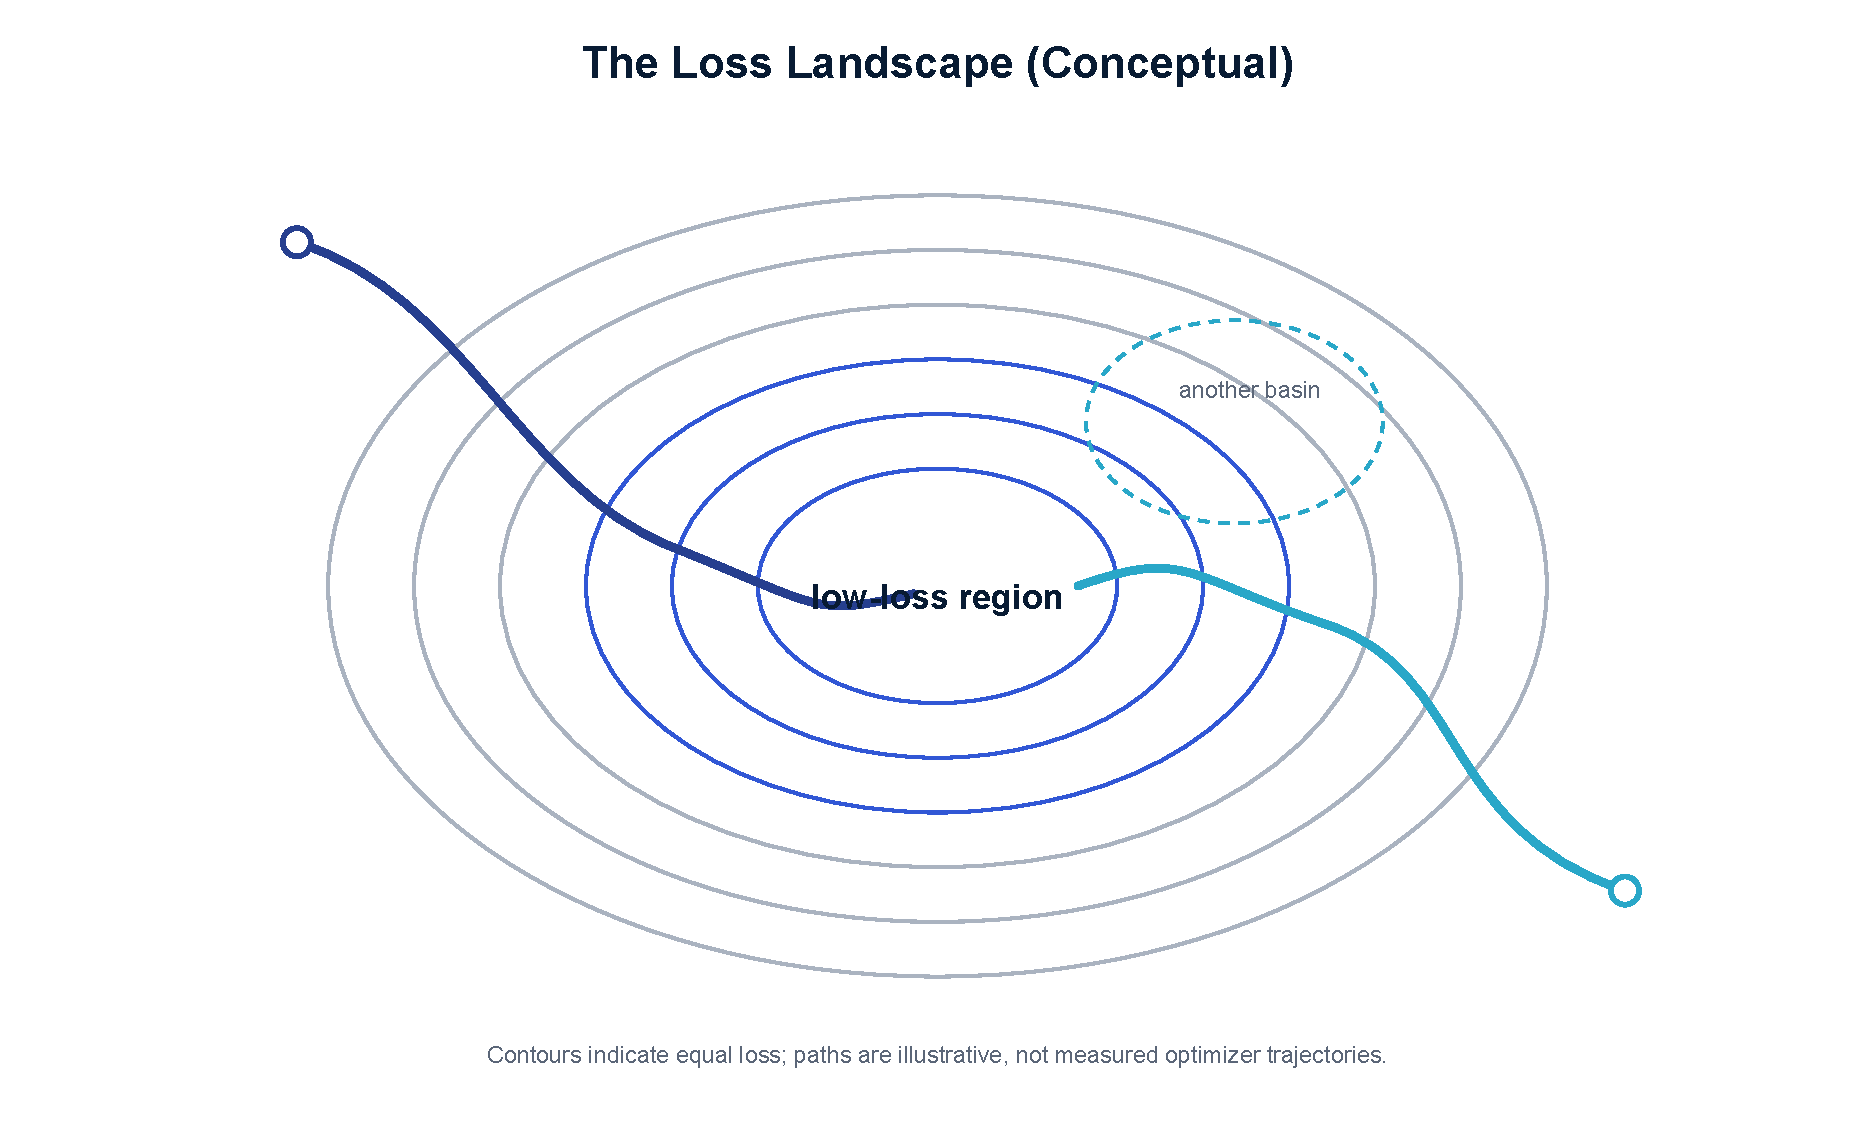
\includegraphics[width=\linewidth,height=.72\textheight,keepaspectratio]{chapters/../assets/figures/fig-3-1-loss-landscape.pdf}
\caption*{\textbf{Figure 3.1:} The Loss Landscape. \emph{The loss function defines
a surface in weight space. Training is navigation toward a valley. The
shape of the terrain determines which strategies work.}}
\addcontentsline{lof}{figure}{\protect\numberline{3.1}The Loss Landscape. The loss function defines a surface in weight space. Training is navigation toward a valley. The shape of the terrain determines which strategies work.}
\label{figure-3-1}
\end{figure}
\FloatBarrier

\subsection{The Gradient: Reading the Slope of the
Terrain}\label{the-gradient-reading-the-slope-of-the-terrain}

The gradient of the loss function is the mathematical equivalent of
reading the slope of the terrain at your current location. If you are
standing on a hillside and want to walk downhill as efficiently as
possible, you look at the slope in every direction and choose the
direction that descends most steeply. The gradient tells you exactly
that: for each weight in the network, it tells you how much the loss
would change if you increased that weight slightly. A large positive
gradient value means "increasing this weight would significantly
increase the loss" --- which means decreasing it slightly will decrease
the loss.

The update rule is elegantly simple. At each step, we compute the
gradient and move a small amount in the opposite direction --- downhill:

\[
w_{t+1} = w_t - \eta\,\nabla_w L(w_t)
\]

This single equation, applied to millions of weights simultaneously, is
the beating heart of all neural network training. Every training step is
a small, coordinated downhill nudge of the entire weight space. Over
thousands of iterations, these nudges compound --- and the network
improves.

\subsection{The Learning Rate Dilemma: How Big Should Each Step
Be?}\label{the-learning-rate-dilemma-how-big-should-each-step-be}

The learning rate --- the scalar that controls how much we adjust the
weights at each step --- is one of the most consequential
hyperparameters in training. The analogy to step size on a hillside is
almost perfect:

If your steps are too large, you will overshoot the valley. You might
approach a minimum, then step directly over it to the other side, then
overshoot back --- bouncing endlessly across the bottom without ever
settling in. In extreme cases, the steps are so large that the network
diverges entirely: the loss explodes rather than decreases.

If your steps are too small, you will eventually reach the valley, but
it will take an impractical amount of time. In practice, with millions
of weights and billions of training examples, "too slow" means "too
expensive" --- days or weeks of computation time instead of hours.

A just-right learning rate descends steadily --- fast enough to make
progress, small enough to settle accurately into a minimum. Finding this
balance is part art, part systematic exploration. The loss curves in
Figure 3.4 illustrate what each scenario looks like in practice: a key
skill this chapter develops.

\begin{figure}[htbp]
\centering
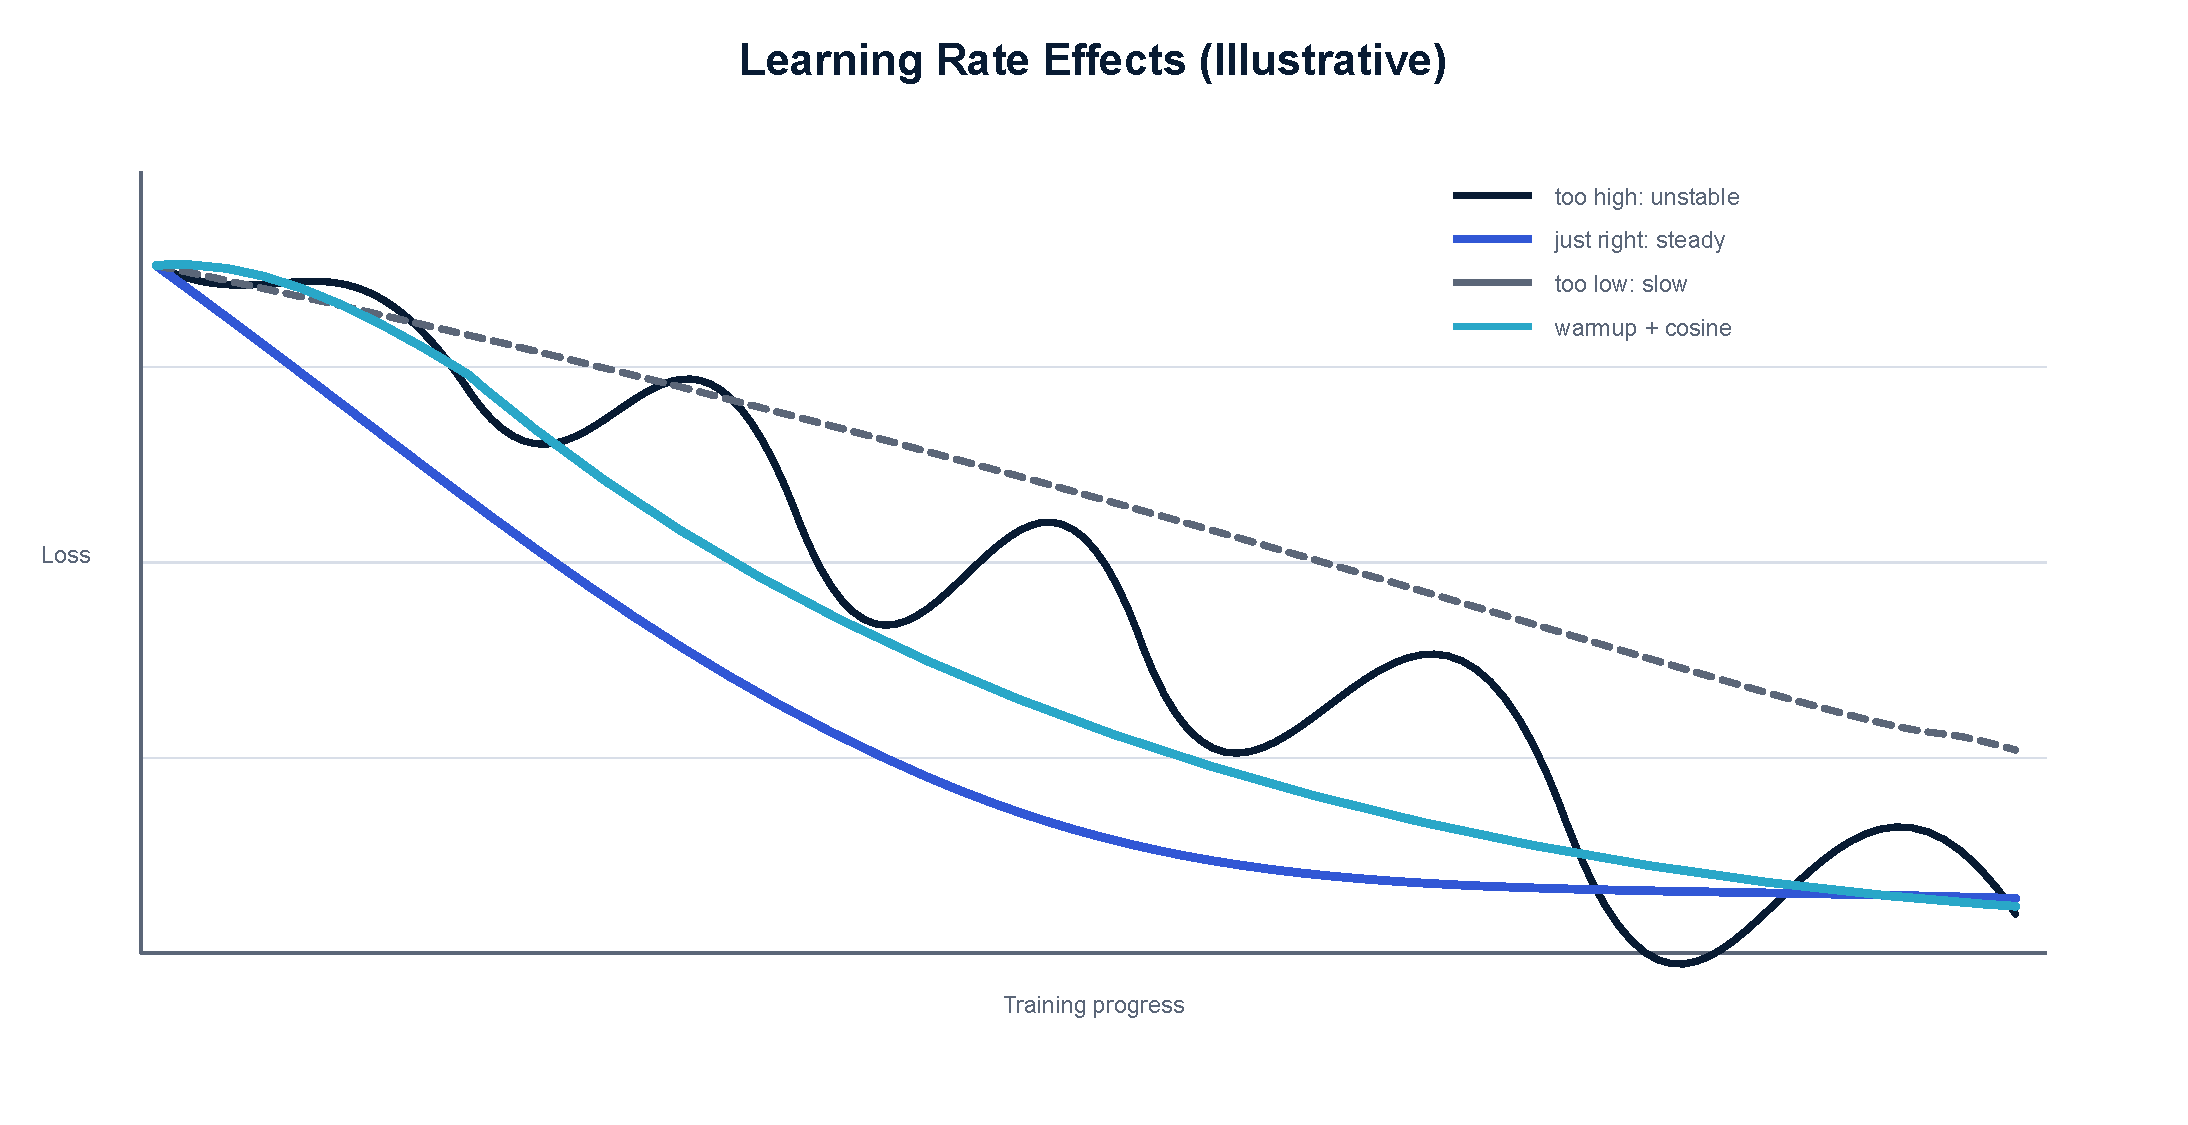
\includegraphics[width=\linewidth,height=.72\textheight,keepaspectratio]{chapters/../assets/figures/fig-3-4-learning-rate-effects.pdf}
\caption*{\textbf{Figure 3.4:} Learning Rate Effects. \emph{The learning rate is
arguably the single most important hyperparameter. Learn to read its
signature in the training curve.}}
\addcontentsline{lof}{figure}{\protect\numberline{3.4}Learning Rate Effects. The learning rate is arguably the single most important hyperparameter. Learn to read its signature in the training curve.}
\label{figure-3-4}
\end{figure}
\FloatBarrier

\subsection{Backpropagation: Tracing Responsibility
Backward}\label{backpropagation-tracing-responsibility-backward}

Computing the gradient of the loss with respect to a single weight seems
straightforward: nudge the weight, see how the loss changes. But a deep
network might have millions of weights. Computing the gradient by
nudging each weight individually would require millions of forward
passes per training step --- completely impractical.

Backpropagation is the algorithm that computes all these gradients
simultaneously in a single efficient backward pass through the network.
The key insight is the chain rule of calculus: the gradient of the loss
with respect to any weight can be decomposed into a chain of local
gradients --- how much did this weight affect this
layer\textquotesingle s output? How much did that output affect the next
layer\textquotesingle s output? How much did the final
layer\textquotesingle s output affect the loss?

Think of it as a chain of accountability. When the network makes an
error, backpropagation answers the question: "How much was each weight
responsible for this mistake?" A weight that was heavily involved in
producing the wrong answer receives a large gradient --- a strong signal
to change. A weight that played a minor role receives a small gradient
--- a gentle nudge, if any.

This credit-assignment mechanism is why deep networks can learn at all.
Without backpropagation, there would be no principled way to tell the
network which of its millions of parameters caused the error. With it,
every weight in every layer receives exactly the feedback it is
responsible for.

\begin{longtable}[]{@{}
  >{\raggedright\arraybackslash}p{(\linewidth - 0\tabcolsep) * \real{1.0014}}@{}}
\toprule\noalign{}
\endhead
\bottomrule\noalign{}
\endlastfoot
\textbf{🔗 Connection to Chapter 2}

Recall from Chapter 2 that Sigmoid activation functions produce outputs
between 0 and 1 --- and that their derivatives are near zero at both
extremes. This property becomes critically important during
backpropagation: when the gradient passes through a Sigmoid activation
in saturation, it is multiplied by a near-zero value. Over many layers,
these near-zero multiplications accumulate, and the gradient shrinks
toward nothing. This is the vanishing gradient problem, and it is why
ReLU activations --- which have a gradient of either 0 or 1 --- were
such an important innovation. The architectural choices you learned in
Chapter 2 were not arbitrary: they were solutions to the training
problems we are studying now. \\
\end{longtable}

\subsection{Batch Strategies: How Much Data Per
Update?}\label{batch-strategies-how-much-data-per-update}

Every gradient update requires us to compute the loss over some number
of training examples. How many examples should we use per update? This
choice --- the batch size --- involves a fundamental tradeoff between
gradient accuracy and computational speed.

\subsection{Batch Gradient Descent: The Careful
Surveyor}\label{batch-gradient-descent-the-careful-surveyor}

Use every training example to compute each gradient update. The gradient
estimate is maximally accurate --- it reflects the true slope of the
loss landscape over the full dataset. But with millions of training
examples, computing one update requires a full pass through all of them.
Training is impractically slow. This approach is rarely used in
practice.

\subsection{Stochastic Gradient Descent: The Impulsive
Explorer}\label{stochastic-gradient-descent-the-impulsive-explorer}

Use a single randomly chosen training example per update. Training is
extremely fast --- the network updates with every example. But the
gradient estimate is highly noisy: a single example might be atypical,
and the resulting update might send the weights in the wrong direction.
Training is erratic, bouncing around the loss landscape rather than
descending smoothly. The noise is not always bad --- it can help the
optimizer escape shallow local minima --- but it makes convergence
unpredictable.

\subsection{Mini-Batch Gradient Descent: The Focus
Group}\label{mini-batch-gradient-descent-the-focus-group}

Use a small batch of examples --- typically 32 to 256 --- per update.
Think of it as conducting a focus group before making a product
decision. One customer\textquotesingle s opinion is too noisy to act on.
Surveying all customers before making any decision is too slow. Twelve
to thirty-two people in a room gives you a representative, actionable
signal efficiently.

Mini-batch is the dominant approach in modern deep learning. It is fast
enough to train on enormous datasets, accurate enough to converge
reliably, and just noisy enough to provide the regularizing effect that
helps networks generalize. GPU hardware is also designed to process
batches of examples in parallel --- making mini-batch training
dramatically faster than stochastic updates on modern hardware.

\begin{figure}[htbp]
\centering
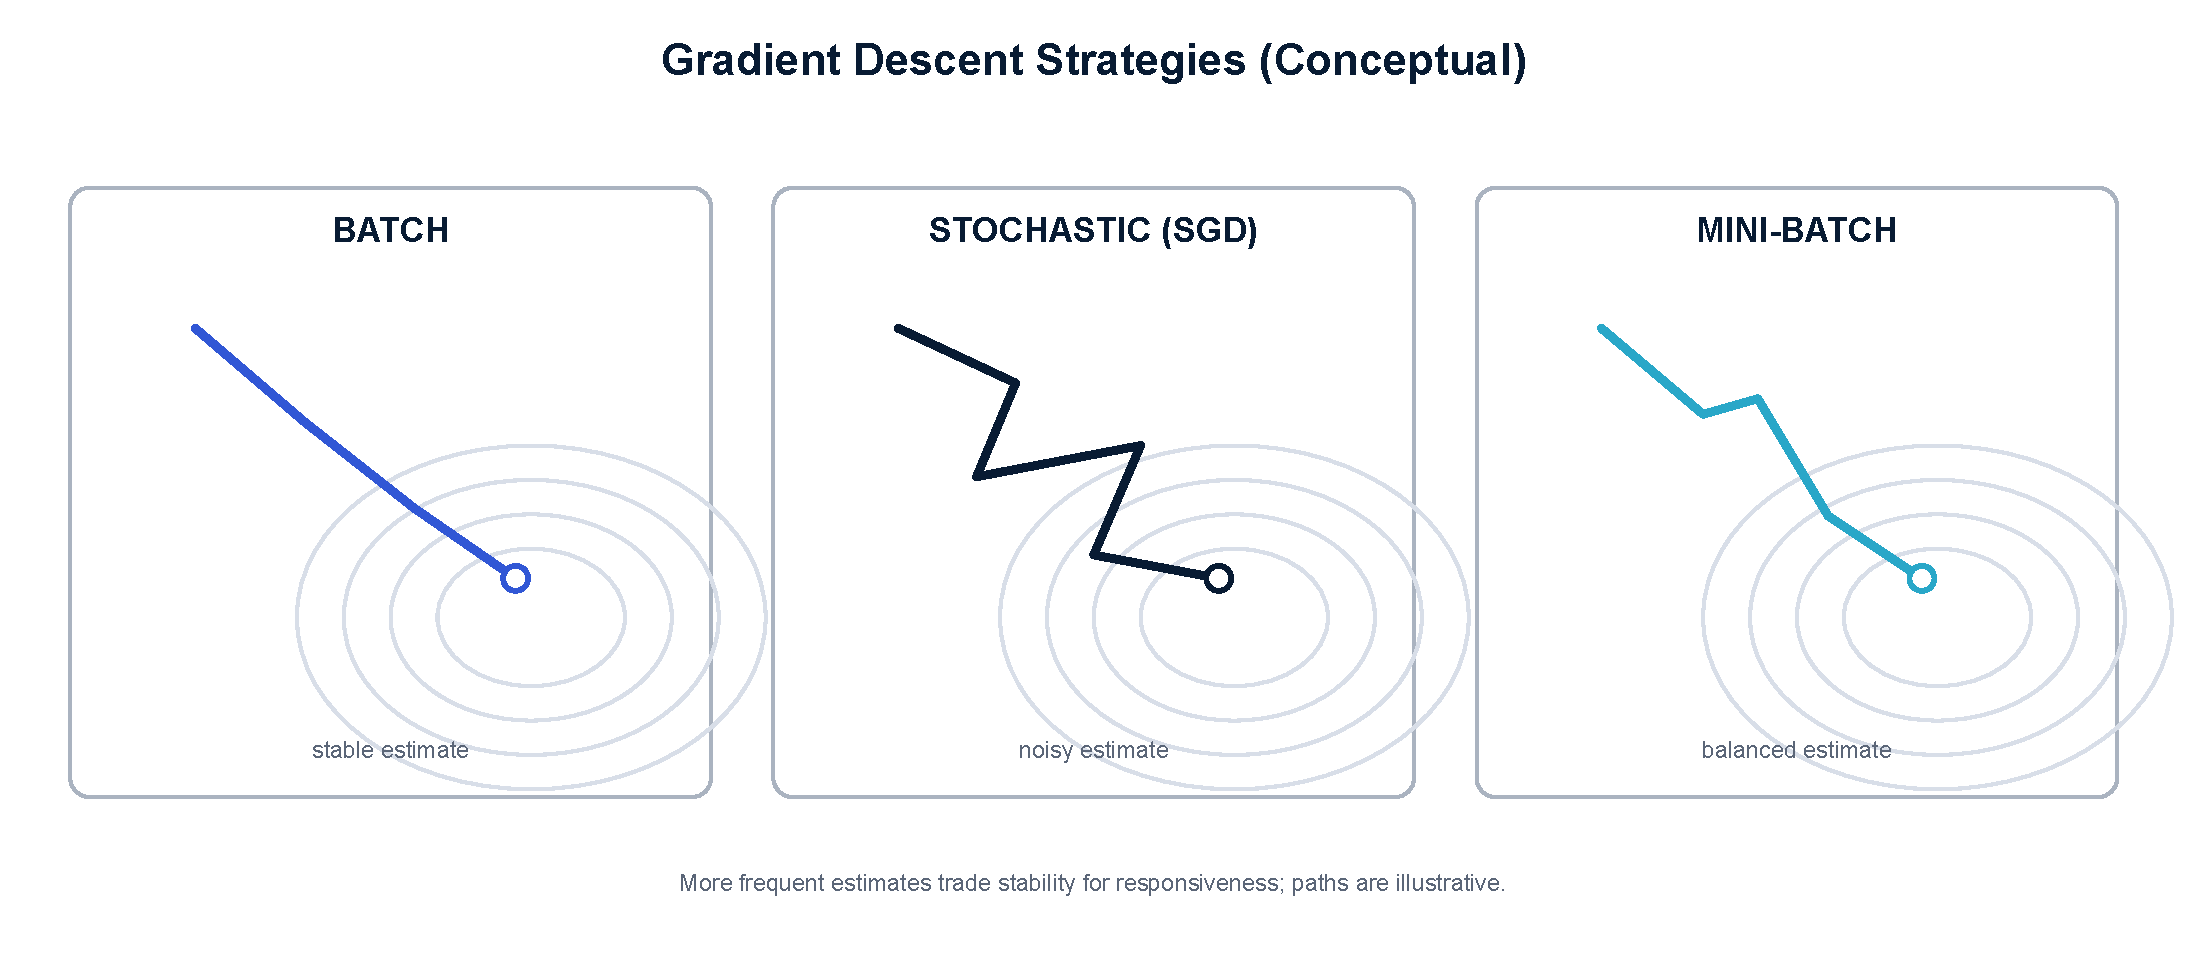
\includegraphics[width=\linewidth,height=.72\textheight,keepaspectratio]{chapters/../assets/figures/fig-3-5-batch-strategies.pdf}
\caption*{\textbf{Figure 3.5:} Batch Strategies. \emph{Noisier gradient estimates
produce more erratic paths --- but sometimes a little noise helps escape
shallow traps.}}
\addcontentsline{lof}{figure}{\protect\numberline{3.5}Batch Strategies. Noisier gradient estimates produce more erratic paths — but sometimes a little noise helps escape shallow traps.}
\label{figure-3-5}
\end{figure}
\FloatBarrier

\subsection{Modern Optimizers: Smarter Ways to
Descend}\label{modern-optimizers-smarter-ways-to-descend}

Basic gradient descent uses the same step size for every weight at every
moment. But different weights deserve different treatment. A weight that
has been oscillating rapidly should perhaps receive smaller updates ---
its gradient is unstable and large steps will worsen the oscillation. A
weight whose gradient has been consistently pointing in one direction
can perhaps afford a larger step --- momentum is building, and the
landscape is clearly sloping in a consistent direction.

Modern optimizers incorporate these intuitions automatically:

\begin{longtable}[]{@{}
  >{\raggedright\arraybackslash}p{(\linewidth - 2\tabcolsep) * \real{0.0889}}
  >{\raggedright\arraybackslash}p{(\linewidth - 2\tabcolsep) * \real{0.9062}}@{}}
\toprule\noalign{}
\endhead
\bottomrule\noalign{}
\endlastfoot
\textbf{Optimizer} & \textbf{How It Works and When to Use It} \\
SGD with Momentum & Adds a velocity term that accumulates in directions
where gradients have been consistent. Like a ball rolling downhill,
momentum carries the optimizer forward through flat regions and prevents
oscillation in steep ones. Often produces the best final performance on
well-tuned computer vision problems. \\
Adam (Adaptive Moment Estimation) & Maintains per-parameter learning
rates that adapt based on a running average of recent gradient
magnitudes. Weights with small, consistent gradients get a relatively
large effective step; weights with large, erratic gradients get a
relatively small step. Converges quickly with little tuning. The most
widely-used optimizer for new problems and Transformer models. \\
AdamW & Adam with decoupled weight decay (L2 regularization applied to
weights directly rather than through the gradient). Improves
generalization compared to standard Adam, and is now the preferred
variant in most Transformer training pipelines. \\
RMSprop & Similar to Adam but simpler. Adapts learning rates based on
recent gradient magnitudes alone, without the momentum term. Works well
for RNNs and recurrent architectures. \\
\end{longtable}

No optimizer is universally best. Adam is an excellent starting point
because it requires minimal tuning and often converges quickly. SGD with
momentum sometimes produces better final generalization when carefully
tuned --- it is the dominant choice in state-of-the-art computer vision
training. As you build MIPDS, you will experiment with both.

\section{The Training Loop --- How Learning Actually
Happens}\label{the-training-loop-how-learning-actually-happens}

We now have all the components we need to describe a complete training
run. The training loop is the process that ties everything together:
data, loss function, optimizer, and the model\textquotesingle s weights
--- all coordinated into a repeating rhythm that gradually transforms a
randomly initialized network into a useful one.

\subsection{Before Training Begins: Preparing the
Data}\label{before-training-begins-preparing-the-data}

Good training requires careful data preparation. Two practices are
non-negotiable and one common pitfall must be actively avoided.

\subsection{The Three-Way Split: Training, Validation, and
Test}\label{the-three-way-split-training-validation-and-test}

Every dataset used for training must be divided into three distinct,
non-overlapping portions:

\begin{itemize}
\item
  The training set (typically 70--80\% of data) is the material the
  model learns from. Gradients are computed on this data, and weights
  are updated based on it.
\item
  The validation set (10--15\%) is used to monitor generalization during
  training. After each epoch, we evaluate the model on the validation
  set --- not to update weights, but to check whether learning is
  transferring to data the model has not seen. This is how we detect
  overfitting early.
\item
  The test set (10--15\%) is kept completely sealed until the end. It is
  used exactly once --- after all training, validation, and
  hyperparameter tuning is complete --- to produce an honest estimate of
  how the model will perform on truly new data. If the test set is
  consulted during development, it is contaminated: it becomes, in
  effect, another validation set, and the reported test performance is
  optimistically inflated.
\end{itemize}

\subsection{Normalization: Speaking the Same
Language}\label{normalization-speaking-the-same-language}

Neural networks learn by comparing --- how different are these weights
from last step? How different is this prediction from the truth? These
comparisons work best when all input features are on similar numerical
scales. Raw image pixels range from 0 to 255; raw financial data might
range from 0.01 to 10 million. Training with these values directly would
cause weights corresponding to large-valued features to dominate the
gradient signal. Normalization converts inputs to a common range ---
typically zero mean and unit variance --- so that every feature has
equal standing in the learning process.

\subsection{The Four-Phase Rhythm: One Training
Iteration}\label{the-four-phase-rhythm-one-training-iteration}

A single training iteration --- processing one mini-batch and updating
the weights once --- follows a strict four-phase sequence. This sequence
will repeat millions of times over the course of a full training run.
Understanding it deeply is the key to diagnosing problems when things go
wrong.

\begin{figure}[htbp]
\centering
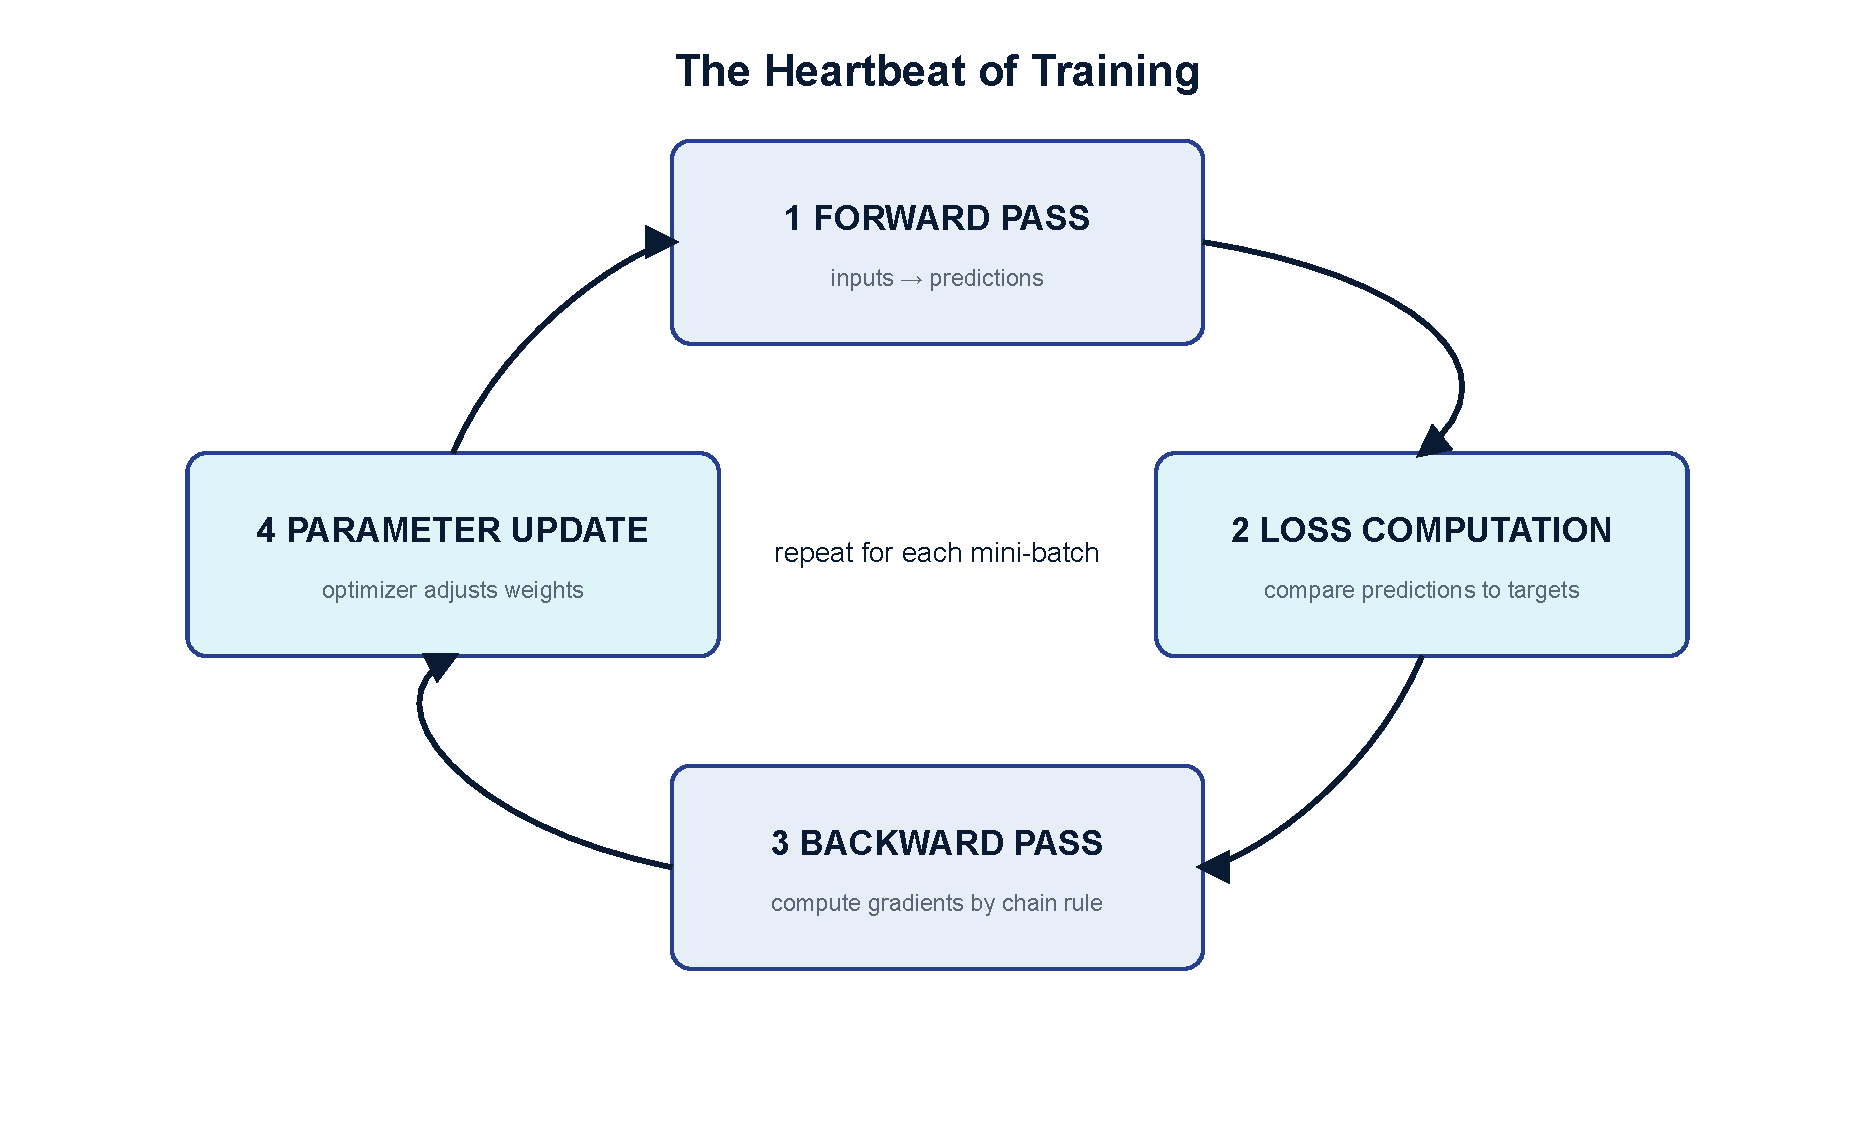
\includegraphics[width=\linewidth,height=.72\textheight,keepaspectratio]{chapters/../assets/figures/fig-3-3-training-loop.pdf}
\caption*{\textbf{Figure 3.3:} The Heartbeat of Training. \emph{This four-phase
loop repeats for every mini-batch in every epoch. Learn to describe each
phase fluently.}}
\addcontentsline{lof}{figure}{\protect\numberline{3.3}The Heartbeat of Training. This four-phase loop repeats for every mini-batch in every epoch. Learn to describe each phase fluently.}
\label{figure-3-3}
\end{figure}
\FloatBarrier

\subsection{Phase 1: The Forward Pass}\label{phase-1-the-forward-pass}

Feed a mini-batch of inputs through the network, layer by layer, from
input to output. Each layer applies its learned transformation ---
matrix multiplication, activation function, normalization --- until the
final layer produces predictions. This is the network doing what it
currently knows how to do, which at the start of training means
producing essentially random outputs.

\subsection{Phase 2: Loss Computation}\label{phase-2-loss-computation}

Compare the batch\textquotesingle s predictions to the ground truth
labels using the loss function. Produce a single scalar value: the
current loss. This number is the entire signal the optimizer will
receive about how the network performed on this batch. High loss means
the predictions were badly wrong. Low loss means they were close.

\subsection{Phase 3: The Backward Pass
(Backpropagation)}\label{phase-3-the-backward-pass-backpropagation}

Propagate the loss signal backward through every layer, computing the
gradient of the loss with respect to every parameter in the network. At
the end of the backward pass, each weight in the network has an
associated gradient value telling us: "If you increased this weight, the
loss on this batch would change by this much." Gradients that are large
in magnitude indicate weights that had an outsized effect on the error.
Gradients near zero indicate weights that barely mattered.

\subsection{Phase 4: The Parameter
Update}\label{phase-4-the-parameter-update}

Apply the optimizer to update every weight using its gradient. The
optimizer determines exactly how the gradient translates into a weight
change --- accounting for momentum, adaptive learning rates, or weight
decay, depending on which optimizer is chosen. After this step, every
weight has been nudged slightly in the direction that reduces loss. The
optimizer\textquotesingle s state is also updated (e.g., momentum
buffers for Adam) for the next iteration.

\subsection{Epochs, Iterations, and the Shape of a Training
Run}\label{epochs-iterations-and-the-shape-of-a-training-run}

One pass through all the training data --- shuffled and processed batch
by batch --- is called an epoch. Training typically requires many
epochs: the same data is visited repeatedly, each time refining the
weights a little further. Early epochs produce large, rapid
improvements. Later epochs produce smaller, more careful adjustments.

How many epochs does training require? There is no universal answer ---
it depends on dataset size, model complexity, learning rate, and the
problem\textquotesingle s difficulty. This is one reason why monitoring
training curves is essential: rather than training for a predetermined
number of epochs and hoping for the best, good practitioners watch the
learning curves and stop when validation performance plateaus or begins
to worsen.

\subsection{Learning Rate Schedules: Adjusting the Pace Over
Time}\label{learning-rate-schedules-adjusting-the-pace-over-time}

A fixed learning rate throughout training is rarely optimal. Early in
training, the network\textquotesingle s weights are far from their ideal
values, and large steps help cover ground quickly. Later in training, as
weights approach a good solution, large steps will cause the optimizer
to overshoot and oscillate rather than settle. The ideal learning rate
changes across training --- and learning rate schedules formalize this
intuition.

\begin{figure}[htbp]
\centering
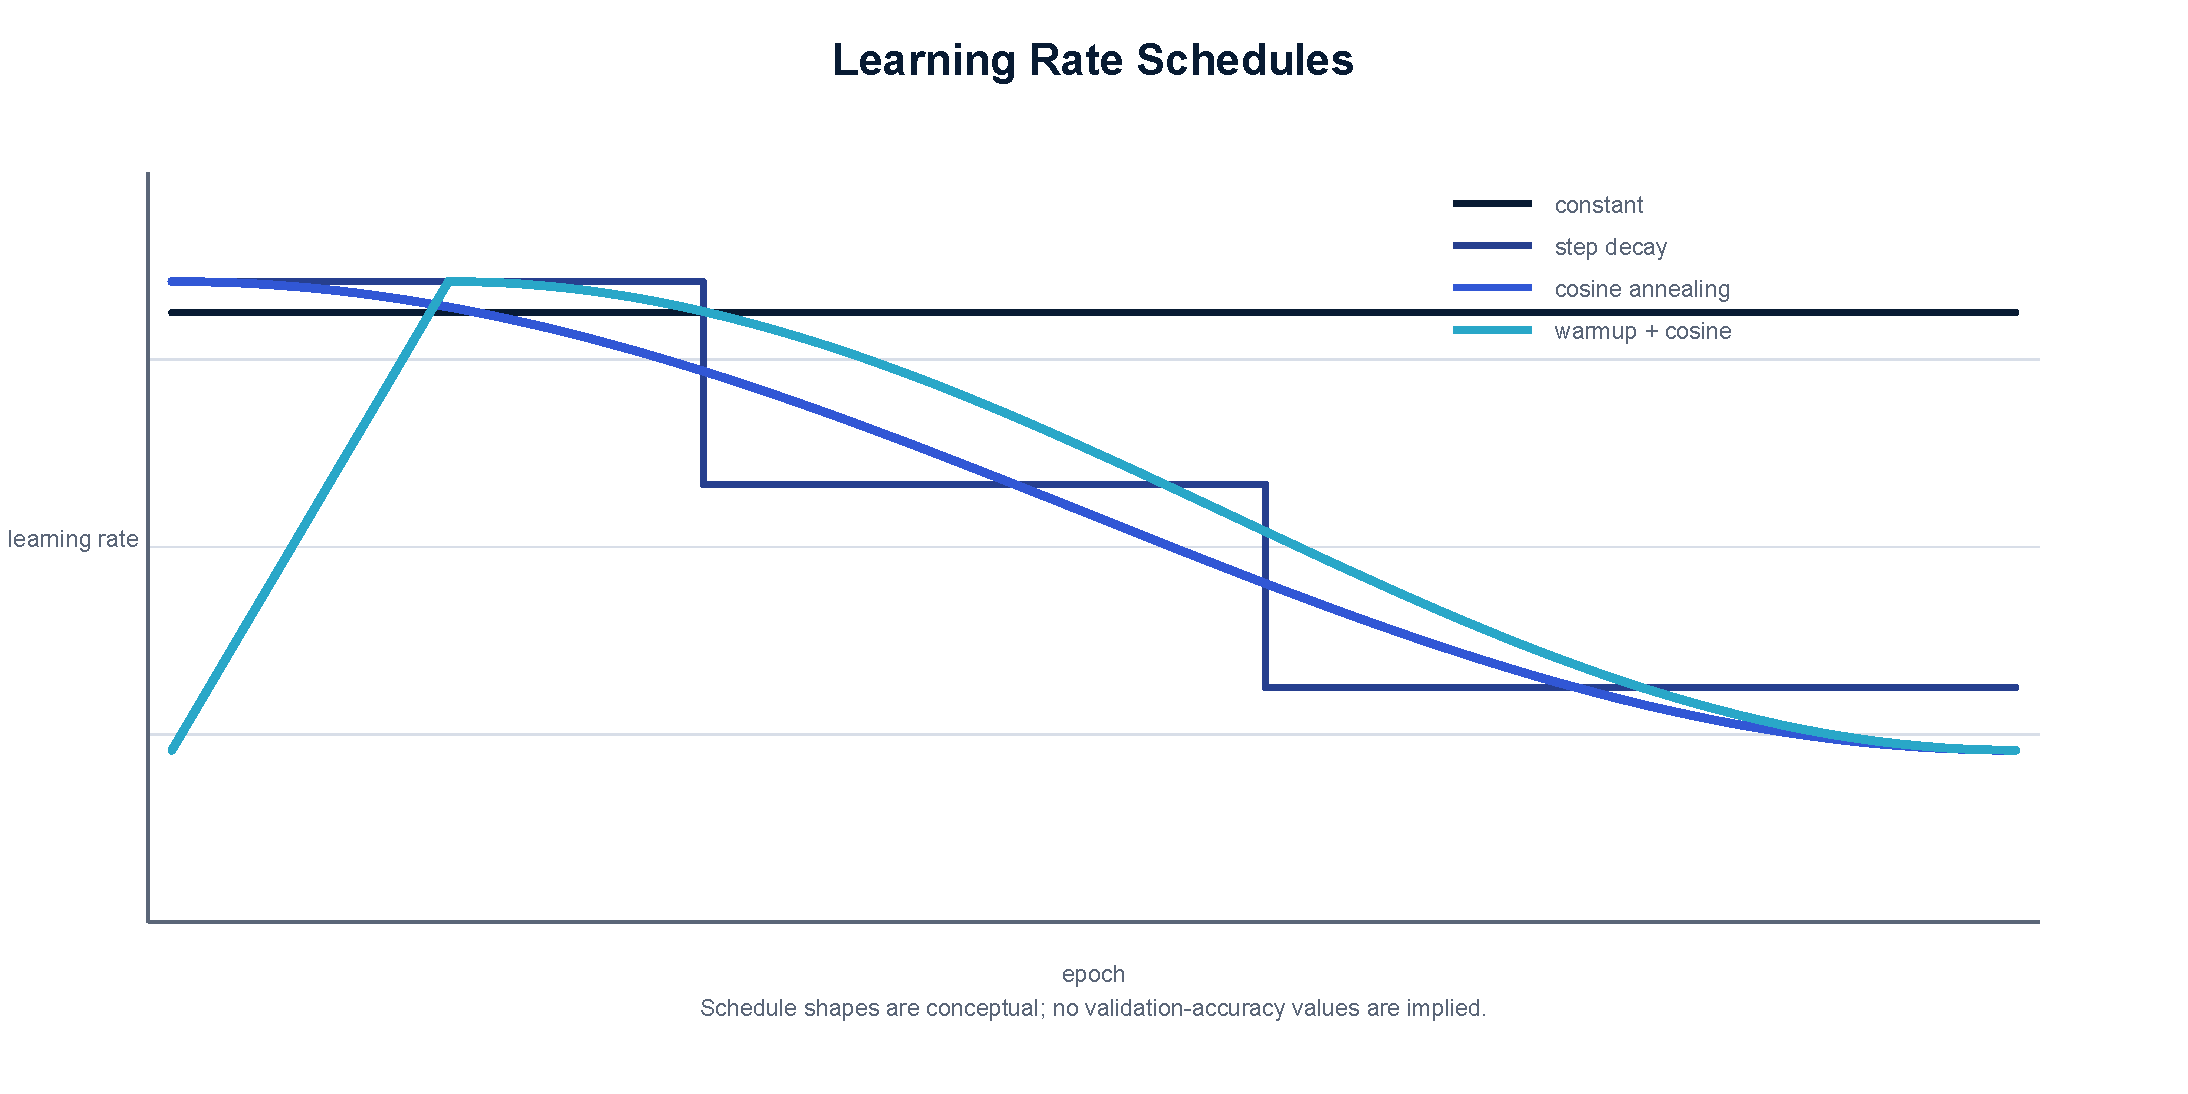
\includegraphics[width=\linewidth,height=.72\textheight,keepaspectratio]{chapters/../assets/figures/fig-3-9-learning-rate-schedules.pdf}
\caption*{\textbf{Figure 3.9:} Schedule Comparison. \emph{Different learning-rate
schedules produce distinct optimization trajectories. Their
effectiveness depends on model architecture, dataset, optimizer, and
training conditions.}}
\addcontentsline{lof}{figure}{\protect\numberline{3.9}Schedule Comparison. Different learning-rate schedules produce distinct optimization trajectories. Their effectiveness depends on model architecture, dataset, optimizer, and training conditions.}
\label{figure-3-9}
\end{figure}
\FloatBarrier

\subsection{Step Decay}\label{step-decay}

The simplest schedule: reduce the learning rate by a fixed factor at
predetermined points in training. For example, start at 0.1, divide by
10 at epoch 30, and again at epoch 60. Training makes rapid early
progress and then consolidates gains at lower rates. The abrupt steps
can sometimes cause instability around the transition points.

\subsection{Cosine Annealing}\label{cosine-annealing}

Rather than sharp steps, cosine annealing decreases the learning rate
smoothly following a cosine curve --- from its maximum value to near
zero across the training run. Its smooth deceleration avoids abrupt
schedule transitions, although its effectiveness depends on the model,
data, optimizer, and training conditions. Cosine annealing can also be
combined with warm restarts: periodically resetting the learning rate
back to its maximum value, allowing the optimizer to leave shallow local
minima and explore different regions of the loss landscape before
decelerating again.

\subsection{Warmup: Easing Into
Learning}\label{warmup-easing-into-learning}

Starting training with the full target learning rate can be
destabilizing, particularly for large networks with large batch sizes.
Weight initialization produces diverse activations, and large initial
gradient steps can push the network to a poor starting configuration
from which it struggles to recover. A warmup period addresses this by
beginning training with a very small learning rate --- sometimes as low
as 1e-8 --- and gradually increasing it to the target value over the
first few epochs.

Warmup is especially important for Transformer models, which are
sensitive to early training instability. You will encounter it again
prominently in Week 8, when we add the language understanding component
to MIPDS. Designing the warmup schedule now is one reason the MIPDS
training infrastructure is built to be modular and extensible.

\subsection{Model Checkpointing: Never Losing
Progress}\label{model-checkpointing-never-losing-progress}

Deep learning training runs can take hours, days, or even weeks.
Hardware failures, power interruptions, or simply realizing midway
through that validation performance was best twenty epochs ago --- all
of these create a need to save progress periodically and recover
specific past states.

A checkpoint is a saved snapshot of the network\textquotesingle s
weights (and optionally the optimizer\textquotesingle s state) at a
specific moment. Most training pipelines save checkpoints at regular
intervals --- every epoch, or whenever the validation loss reaches a new
best. The checkpoint at peak validation performance is typically the
version deployed, even if training continued afterward, since later
epochs may overfit the training data.

\section{Keeping the Model Honest --- Generalization and
Regularization}\label{keeping-the-model-honest-generalization-and-regularization}

The most common failure mode in deep learning is not that a model fails
to learn. It is that a model learns the wrong thing: the specific
details and quirks of its training data rather than the general patterns
that make predictions valuable.

This failure is called overfitting, and understanding it --- together
with the complementary failure of underfitting --- is one of the most
important intuitions you will develop in this course. The techniques
designed to prevent overfitting are collectively called regularization.

\subsection{The Generalization
Problem}\label{the-generalization-problem}

Consider the difference between a student who truly understands calculus
and one who has memorized every problem in the textbook. On exam
questions drawn from the textbook, both students will do well. On a
novel problem that requires applying the same underlying principles ---
slightly differently presented, in an unfamiliar context --- the genuine
understander thrives and the memorizer struggles.

A neural network faces exactly this challenge. Its training data is a
finite sample from the infinite real world. The patterns in that sample
are part genuine signal (the features that actually distinguish cats
from dogs) and part noise (the specific lighting of the
photographer\textquotesingle s studio, the particular background in
which this dog was photographed, the compression artifacts in this
image). A model with sufficient capacity can learn both. The goal is to
learn the signal and discard the noise.

Generalization is the ability to apply what was learned from training
data to new, unseen data. Validating on a held-out set during training
is how we measure it continuously. The gap between training performance
and validation performance is the primary diagnostic for whether a model
has generalized.

\subsection{Overfitting: When Your Model Becomes a
Memorizer}\label{overfitting-when-your-model-becomes-a-memorizer}

Overfitting occurs when the model learns the training data too precisely
--- including its noise and idiosyncrasies --- at the expense of
learning general patterns. On a learning curve, overfitting has a
characteristic signature: training loss continues to decrease smoothly
over epochs, while validation loss plateaus and then begins to increase.
The two curves diverge.

The underlying cause is almost always a mismatch between model capacity
and data size or diversity. A very deep, highly parameterized network
applied to a small dataset has the capacity to memorize every training
example --- and it will, if given enough epochs. This is not a sign of
intelligence; it is a sign of overpowered memorization.

\begin{figure}[htbp]
\centering
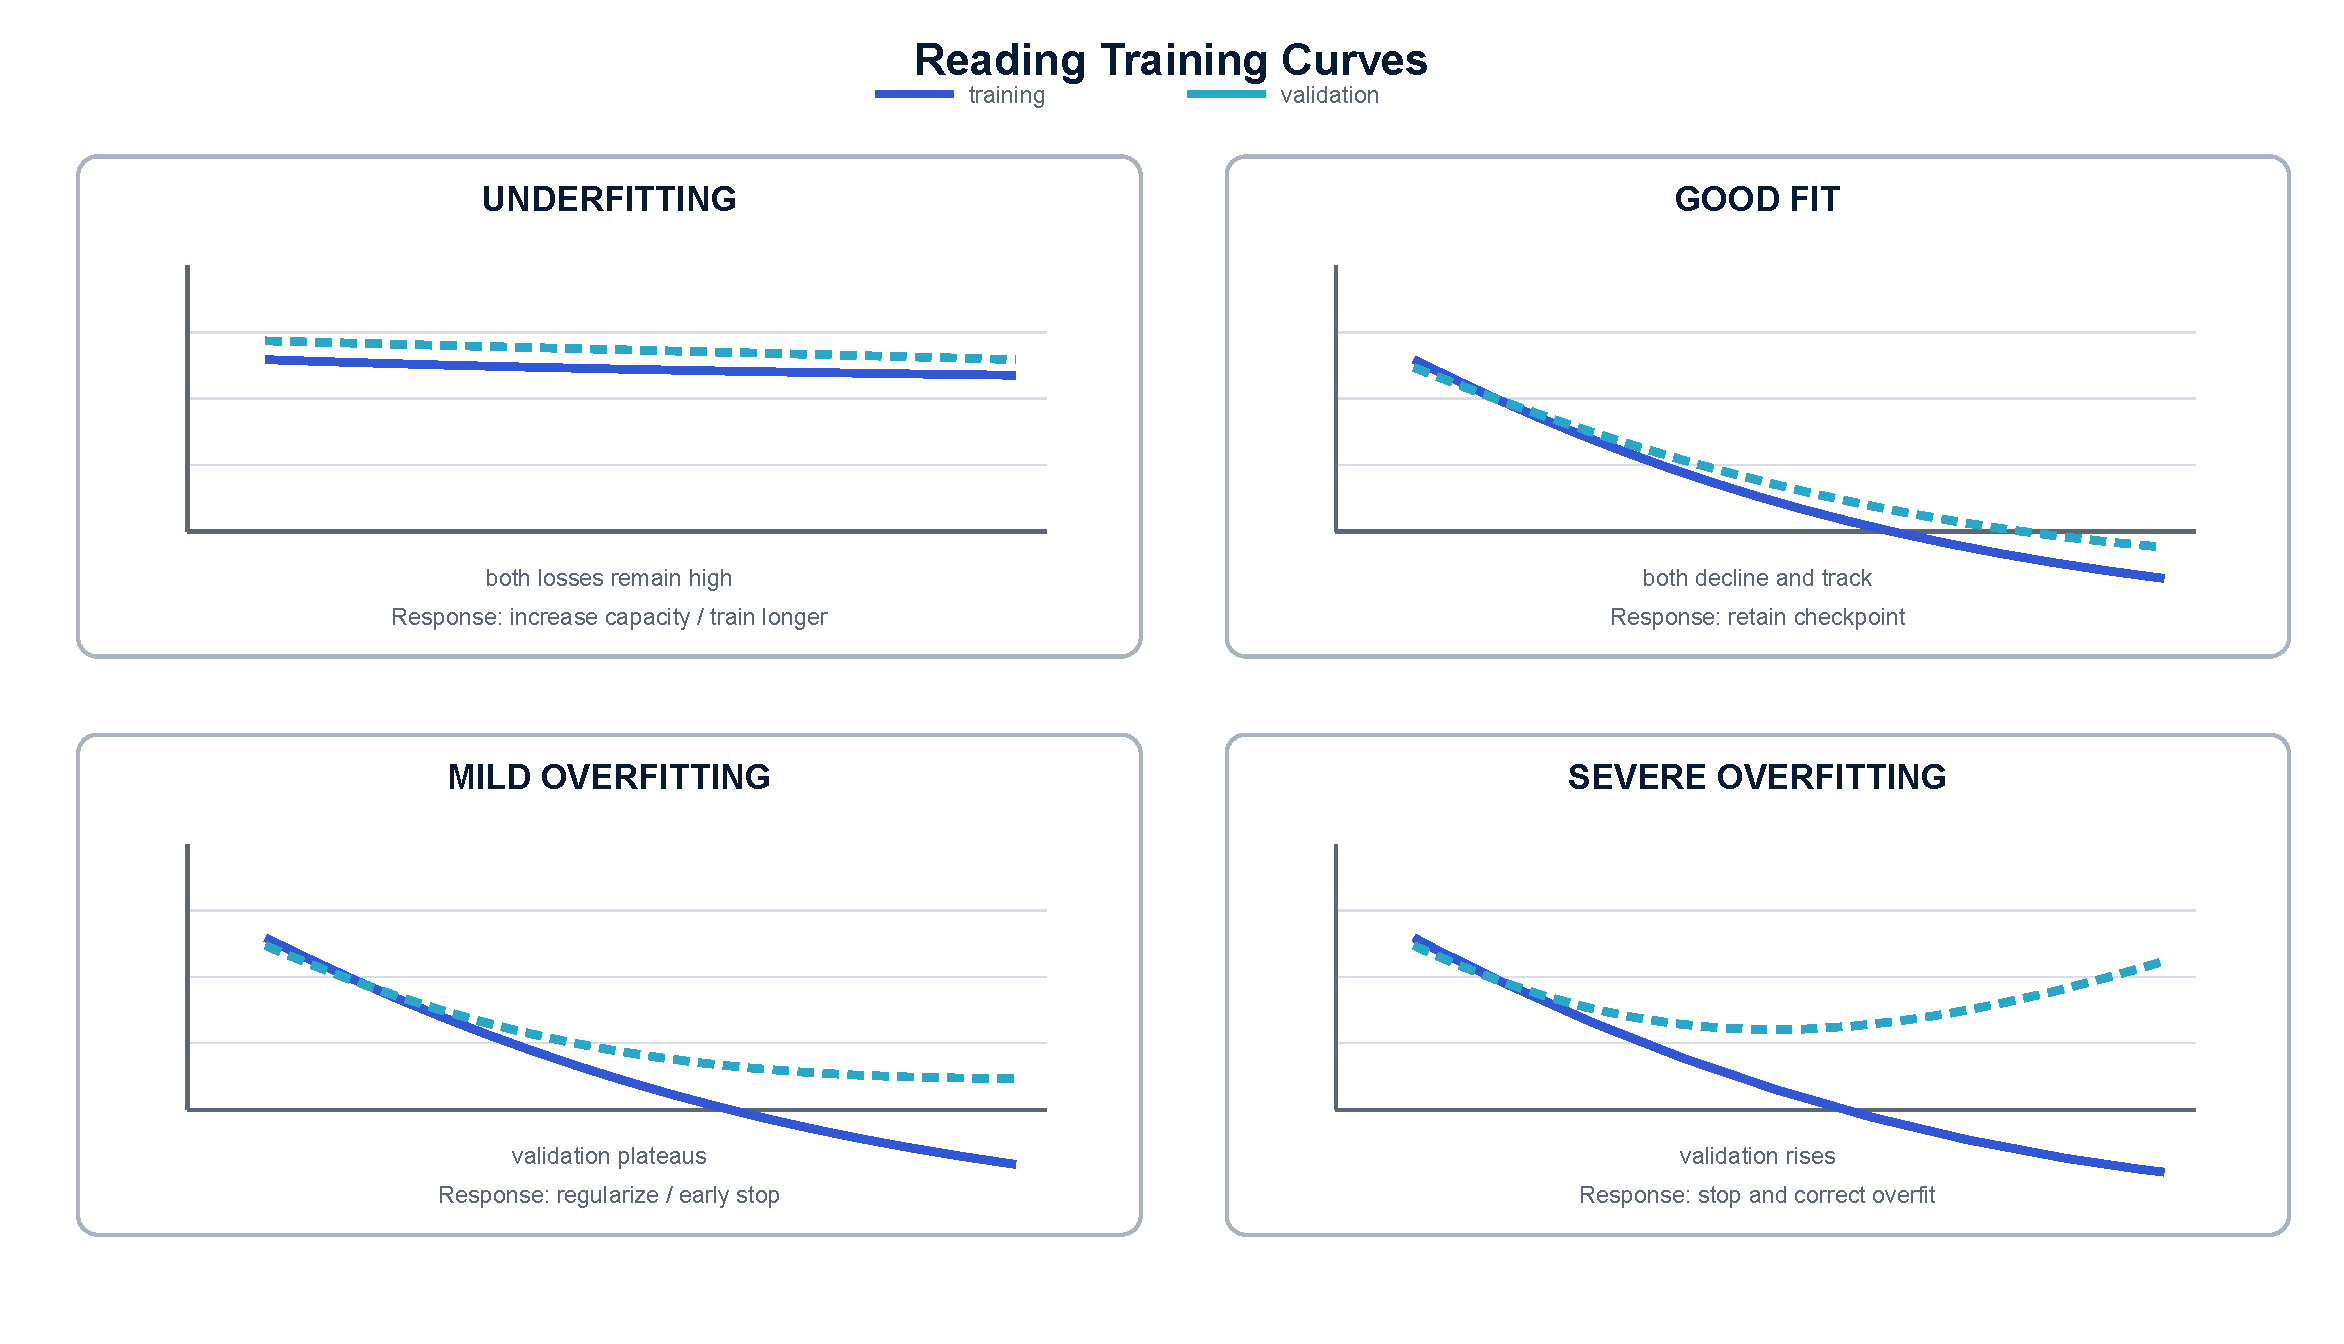
\includegraphics[width=\linewidth,height=.72\textheight,keepaspectratio]{chapters/../assets/figures/fig-3-6-training-curves.pdf}
\caption*{\textbf{Figure 3.6:} Reading Training Curves. \emph{Learn to recognize
these four patterns instantly. Each represents a distinct failure mode
with a distinct remedy.}}
\addcontentsline{lof}{figure}{\protect\numberline{3.6}Reading Training Curves. Learn to recognize these four patterns instantly. Each represents a distinct failure mode with a distinct remedy.}
\label{figure-3-6}
\end{figure}
\FloatBarrier

\subsection{Dropout: Training a Team, Not a
Star}\label{dropout-training-a-team-not-a-star}

Imagine a study group preparing for a demanding exam. If the group
always relies on the same two members to answer the hard questions, the
rest of the team stops engaging seriously --- they can coast on the
stars. But if, before each study session, you randomly designated that
some members must sit out --- so that everyone, at some point, must know
the material independently --- the whole group develops real competence.

Dropout is the neural network equivalent of this arrangement. During
each training step, a randomly selected fraction of neurons ---
typically 20 to 50 percent --- are set to zero. They do not contribute
to the forward pass; they do not receive gradient updates in the
backward pass. The network must solve each training example using a
different random subset of its neurons.

The consequence is powerful: no single neuron can become indispensable.
The network cannot learn "whenever I see this specific pixel pattern in
this specific neuron, predict cat" --- because that neuron will often be
absent. Instead, it must distribute knowledge across many pathways, each
capable of detecting the relevant features independently. The result is
a more robust, redundant representation that generalizes better to new
examples.

At test time, all neurons are active --- but their outputs are scaled
down by the dropout probability to maintain the correct expected
magnitude. No randomness at inference; only robust representations built
during training.

\begin{figure}[htbp]
\centering
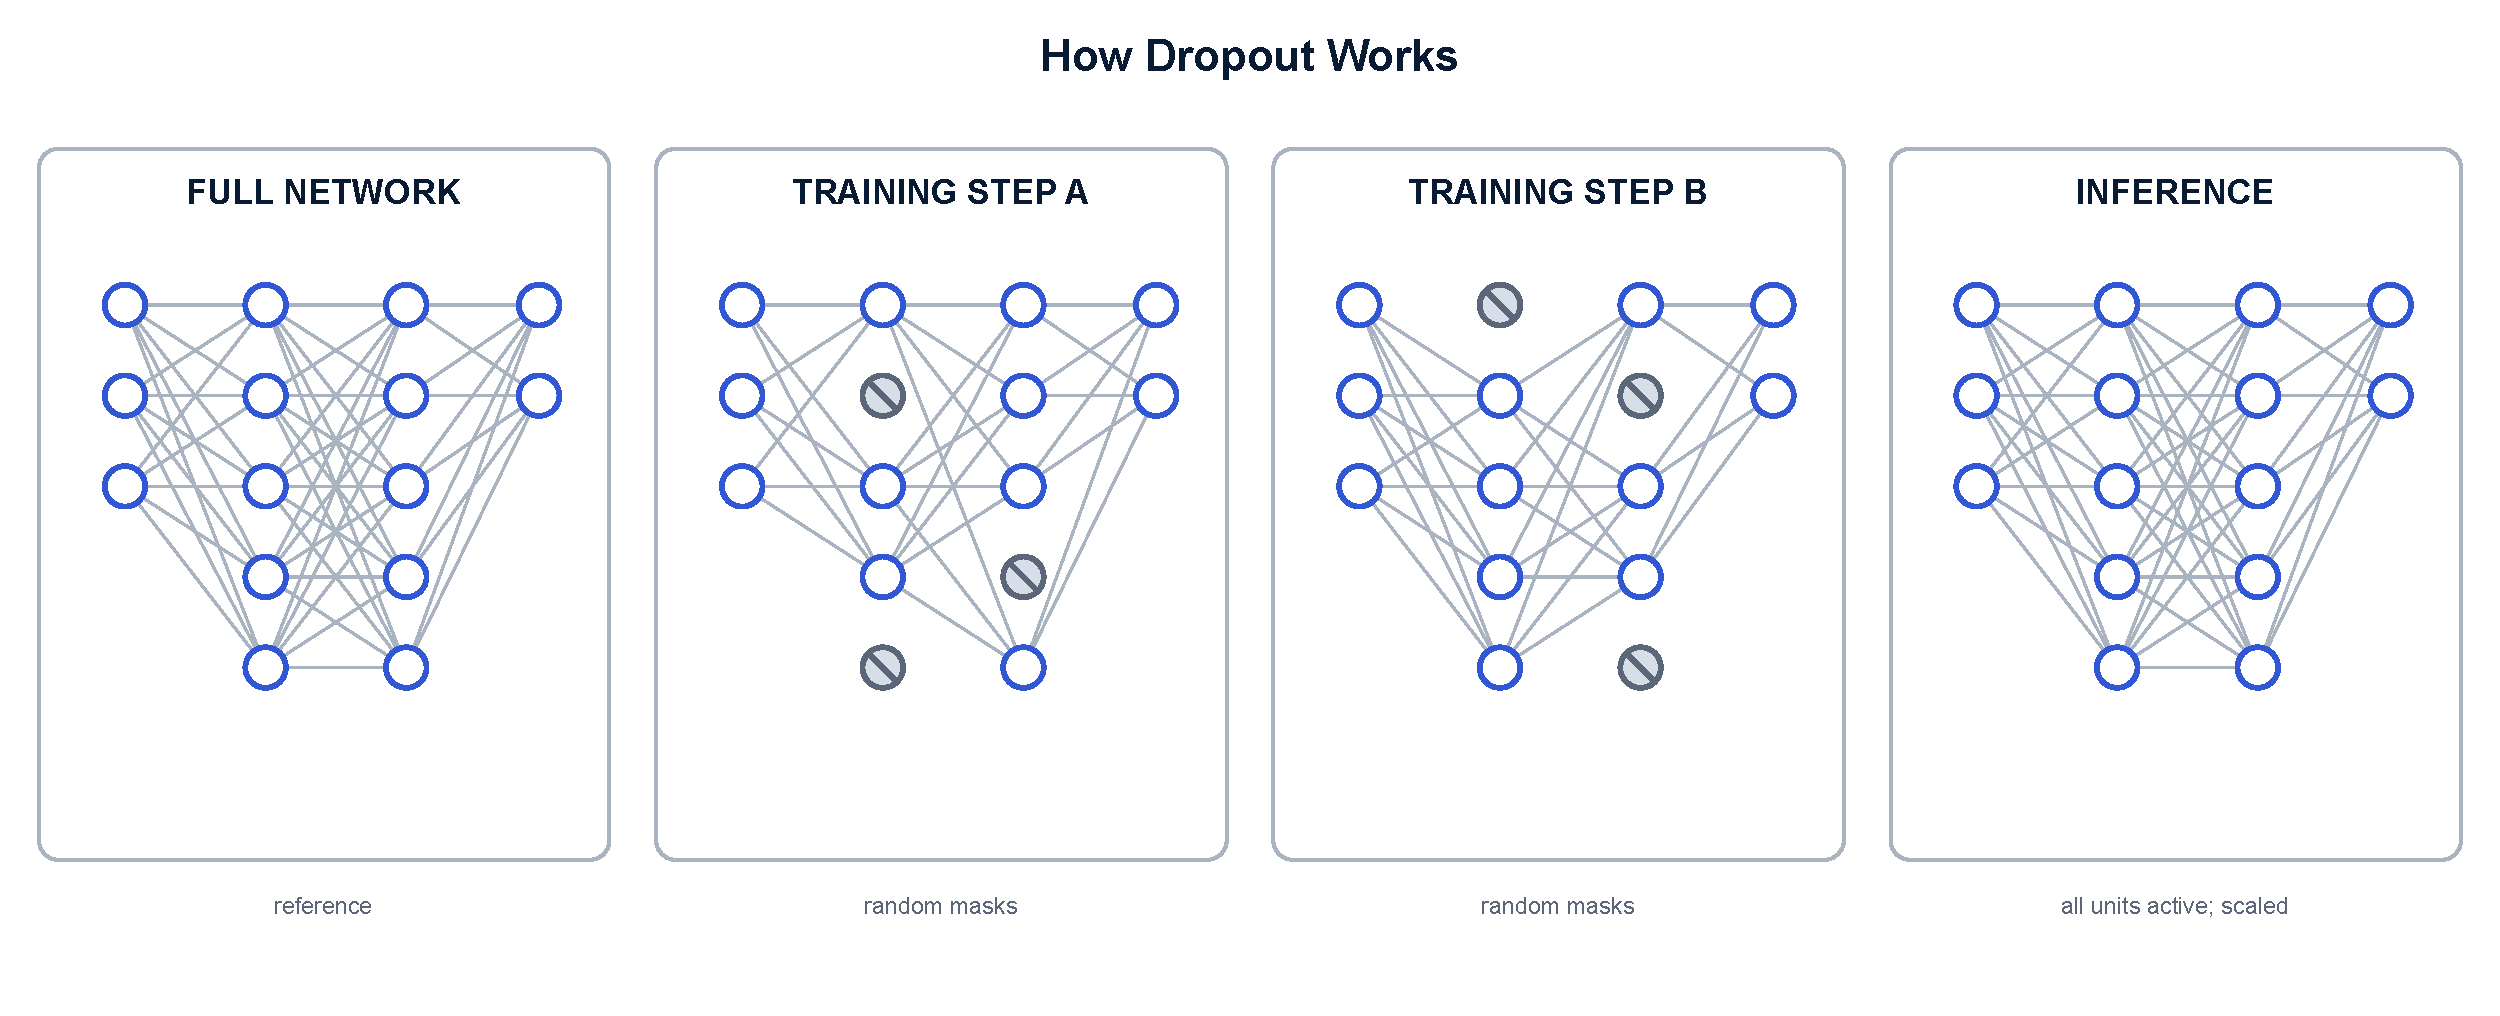
\includegraphics[width=\linewidth,height=.72\textheight,keepaspectratio]{chapters/../assets/figures/fig-3-7-dropout.pdf}
\caption*{\textbf{Figure 3.7:} Dropout. \emph{By randomly silencing neurons during
training, Dropout prevents over-reliance on any single pathway and
forces distributed learning.}}
\addcontentsline{lof}{figure}{\protect\numberline{3.7}Dropout. By randomly silencing neurons during training, Dropout prevents over-reliance on any single pathway and forces distributed learning.}
\label{figure-3-7}
\end{figure}
\FloatBarrier

\subsection{L2 Regularization: Occam\textquotesingle s Razor for Neural
Networks}\label{l2-regularization-occams-razor-for-neural-networks}

The medieval philosopher William of Ockham argued that, among competing
explanations for a phenomenon, the simplest one consistent with the
evidence should be preferred. This principle --- now called
Occam\textquotesingle s Razor --- turns out to be deeply relevant to
machine learning.

A network with very large weights can express very complex,
sharply-curved decision boundaries. Large-weight solutions can fit
training data extremely precisely --- including its noise. But simpler
solutions, with smaller weights, tend to produce smoother, more
generalizable boundaries.

L2 regularization --- also called weight decay --- encodes
Occam\textquotesingle s Razor directly into the training process. It
adds a penalty term to the loss function that is proportional to the sum
of squared weights:

\[
L_{\text{total}} = L_{\text{task}} + \lambda\sum_j w_j^2
\]

The parameter λ (lambda) controls how strongly we enforce simplicity. A
higher λ means a stronger preference for small weights. The optimizer
now has two objectives simultaneously: minimize prediction error, and
keep weights small. This competition produces models that explain the
training data as well as necessary, but no more elaborately than needed.

L1 regularization is a closely related alternative, using the absolute
value of weights rather than the square. Where L2 encourages weights to
be small, L1 encourages many weights to become exactly zero ---
producing sparse networks in which most connections have been
effectively eliminated. L1 is useful when interpretability or
computational efficiency is a priority.

\subsection{Data Augmentation: More Data Without More
Data}\label{data-augmentation-more-data-without-more-data}

One of the most robust solutions to overfitting is also the most
intuitive: more diverse training data. If the model sees enough
variation in its training examples, it cannot memorize individual quirks
--- there are too many variants of each pattern. But collecting and
labeling new data is expensive.

Data augmentation synthetically expands the training set by applying
label-preserving transformations to existing examples. If you are
training an image classifier, a cat photographed from slightly to the
left is still a cat. A horizontally flipped cat is still a cat. A cat
with the brightness reduced by 20\% is still a cat. By randomly applying
these transformations during training, we present the model with a vast,
continuously varying set of examples --- all generated from the original
data at negligible cost.

Standard augmentation operations for images include random horizontal
flips, rotations, crops, zoom, brightness and contrast adjustment, and
color jitter. For specialized domains --- medical imaging, satellite
imagery, audio --- domain-specific augmentations are critical. In chest
X-ray training, for instance, modest random rotations reflect real-world
variation in patient positioning, while aggressive flips (a mirrored
lung is anatomically wrong) are counterproductive.

More recently, advanced augmentation techniques such as Mixup (blending
two training images and their labels smoothly) and CutMix (replacing a
rectangular region of one image with a patch from another) have been
shown to produce strong regularization, forcing the network to attend to
the full image rather than relying on any single distinctive region.

\subsection{Early Stopping: Knowing When to Stop
Learning}\label{early-stopping-knowing-when-to-stop-learning}

The simplest regularization technique is also the most elegant: stop
training when the model stops improving on the validation set.

In the later stages of a long training run, training loss continues to
decrease --- the model is still fitting the training data more
precisely. But validation loss has plateaued or is rising. The model has
already learned the best generalizable representation it is going to
find; it is now beginning to memorize training-specific noise.
Continuing to train is actively counterproductive.

Early stopping monitors the validation loss after each epoch and
terminates training if it has not improved after a specified number of
epochs --- the patience parameter. Combined with checkpointing (saving
the model at the best validation performance), early stopping ensures
that the final deployed model is the best-generalizing version seen
during training, not the most overtrained.

\subsection{Underfitting: When the Model Isn\textquotesingle t Trying
Hard Enough}\label{underfitting-when-the-model-isnt-trying-hard-enough}

The opposite failure mode is underfitting: the model is too simple, or
too undertrained, to capture the meaningful patterns in the data. Both
training and validation performance are poor. No amount of
regularization will fix an underfitting model --- regularization makes
models simpler, but an already-too-simple model needs the opposite.

Underfitting typically signals one of three problems: the model lacks
the capacity to represent the relevant patterns (too few layers, too few
neurons), training has not run long enough for the model to converge, or
the learning rate is so small that progress has effectively stalled. The
fix is straightforward in principle: increase capacity, train longer, or
increase the learning rate.

\begin{longtable}[]{@{}
  >{\raggedright\arraybackslash}p{(\linewidth - 2\tabcolsep) * \real{0.3500}}
  >{\raggedright\arraybackslash}p{(\linewidth - 2\tabcolsep) * \real{0.6250}}@{}}
\toprule\noalign{}
\endhead
\bottomrule\noalign{}
\endlastfoot
\textbf{Failure Mode} & \textbf{Learning Curve Pattern} \\
Overfitting: Too Specific & Training ↓, Validation ↑ \\
Underfitting: Too Simple & Training ↑, Validation ↑ \\
Good Fit: Just Right & Training ↓, Validation ↓ (tracking) \\
\end{longtable}

\section{Monitoring and Debugging --- Reading the Training
Story}\label{monitoring-and-debugging-reading-the-training-story}

A training run without monitoring is like flying without instruments.
The aircraft might be performing beautifully, or it might be silently
descending toward a mountain range --- and without instruments, there is
no way to know until it is too late. Monitoring training is how we stay
in control of a process that we cannot directly observe.

\subsection{Learning Curves: Your Model\textquotesingle s Vital
Signs}\label{learning-curves-your-models-vital-signs}

The primary monitoring tool is the learning curve: a graph of training
loss and validation loss (or accuracy) over training epochs. Plotted
together, these two curves tell a remarkably complete story about what
is happening inside the model.

A healthy training run shows both curves decreasing together, with the
training loss slightly below the validation loss. The gap between them
--- the generalization gap --- indicates how much performance is lost
when moving from seen to unseen data. A small gap is ideal. A widening
gap is the primary signal of overfitting. A large gap that does not
close suggests either insufficient training data or insufficient
regularization.

Validation loss that plateaus early while training loss continues to
decrease may indicate that the model has already extracted all the
generalizable information available in the dataset --- additional
training is overfitting, not learning. Noisy, erratic training curves
often point to a learning rate that is too high, or batches that are too
small to produce stable gradient estimates.

\subsection{The Gradient Pathologies: When the Learning Signal
Breaks}\label{the-gradient-pathologies-when-the-learning-signal-breaks}

Recall the telephone game: a message is whispered from person to person
down a long line. Two things can go wrong. Each person might whisper a
little more softly than the one before --- by the end of the line, the
message is inaudible. Or each person might speak a little louder --- by
the end, the message has become a shout, then a roar, then
unintelligible noise.

During backpropagation, the gradient signal travels backward through
layers in exactly this manner, being multiplied at each layer by local
derivatives. And the same two failure modes can occur.

\begin{figure}[htbp]
\centering
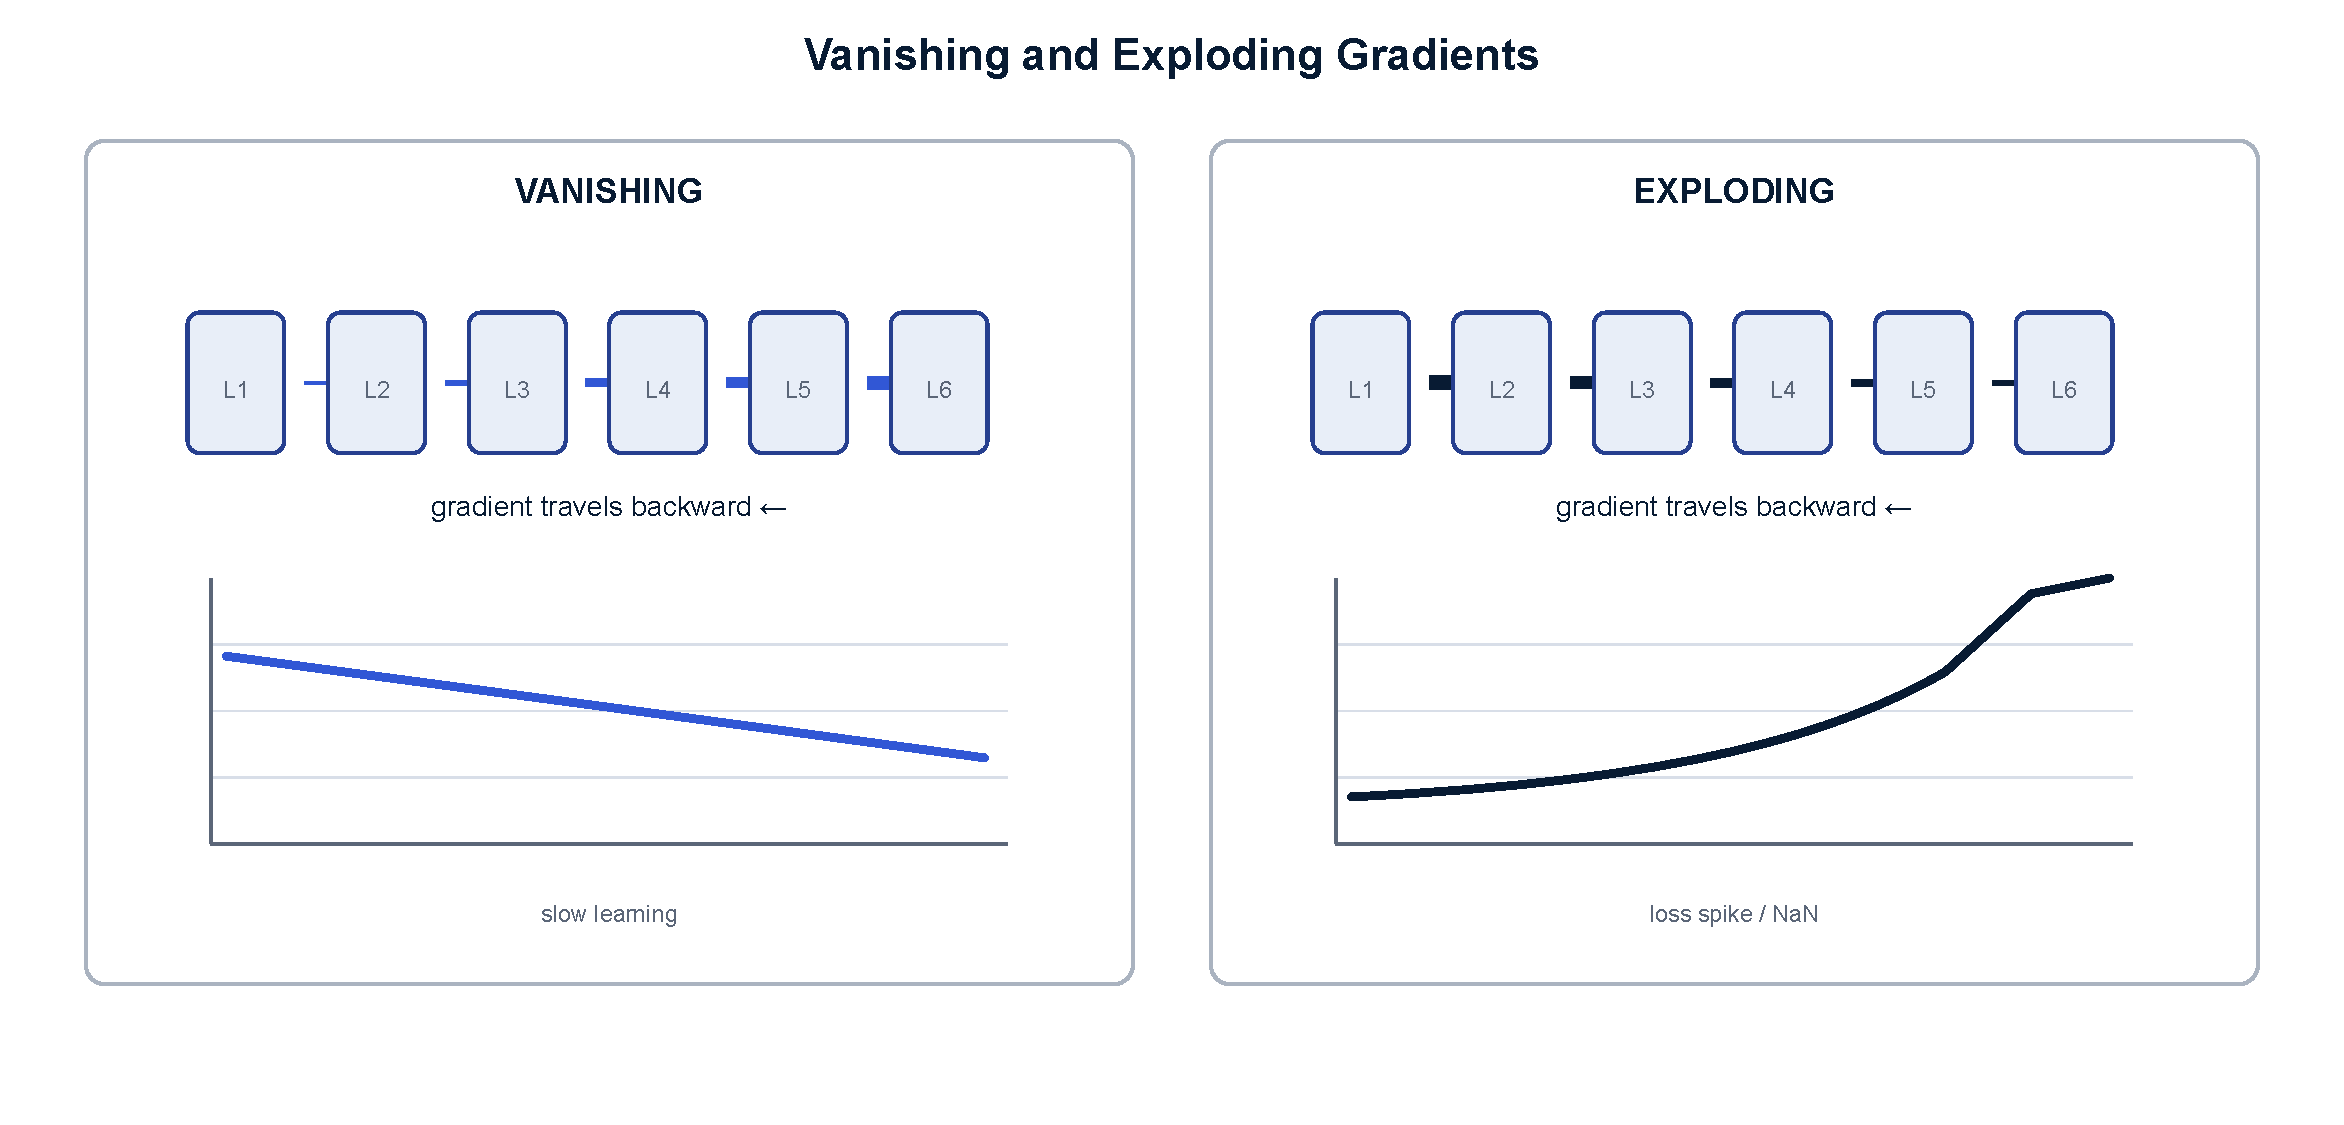
\includegraphics[width=\linewidth,height=.72\textheight,keepaspectratio]{chapters/../assets/figures/fig-3-8-gradient-pathologies.pdf}
\caption*{\textbf{Figure 3.8:} Vanishing and Exploding Gradients. \emph{These
pathologies were among the central technical failures behind the second
AI Winter. Modern architectures and initialization methods largely
solved them --- but they still occur in poorly designed networks.}}
\addcontentsline{lof}{figure}{\protect\numberline{3.8}Vanishing and Exploding Gradients. These pathologies were among the central technical failures behind the second AI Winter. Modern architectures and initialization methods largely solved them — but they still occur in poorly designed networks.}
\label{figure-3-8}
\end{figure}
\FloatBarrier

\subsection{Vanishing Gradients: When Early Layers Stop
Learning}\label{vanishing-gradients-when-early-layers-stop-learning}

When gradients shrink as they travel backward --- due to many
multiplications by small numbers, such as the near-zero derivatives of
saturating activations --- early layers receive an almost imperceptible
signal. Their weights barely change. The network is effectively only
training its later layers. In a very deep network, this means that the
rich, complex hierarchical representations the depth was supposed to
provide are never learned.

The signature of vanishing gradients is subtle: training loss decreases,
but very slowly, and the network fails to reach the performance expected
from its capacity. Early-layer weights show minimal change across
epochs. This was the primary technical obstacle that prevented deep
networks from working before the ReLU revolution and the development of
careful weight initialization strategies.

Fixes include: using ReLU activations (or variants like Leaky ReLU and
GELU) that pass gradients through cleanly; residual connections (which
we will study in depth in Week 4) that provide gradient "shortcuts" from
output directly to early layers; careful weight initialization using
methods like He initialization; and Batch Normalization, which rescales
activations at each layer to maintain a healthy gradient magnitude.

\subsection{Exploding Gradients: When the Learning Signal Goes
Haywire}\label{exploding-gradients-when-the-learning-signal-goes-haywire}

When gradients grow as they travel backward --- each layer amplifying
rather than shrinking the signal --- the optimizer receives weight
updates that are orders of magnitude too large. Weights may jump to
extreme values in a single step. The loss may produce NaN (Not a Number)
values, indicating that numerical overflow has occurred. Training
collapses.

The signature is unmistakable: the training loss, which may have been
decreasing normally, suddenly becomes NaN or spikes to an enormous
value. Gradient clipping --- capping the gradient\textquotesingle s
magnitude at a maximum value before applying it --- is the standard fix.
If the gradient exceeds the clip threshold, it is rescaled to the
threshold rather than applied at full magnitude. Weight initialization
and lower learning rates also help.

\begin{longtable}[]{@{}
  >{\raggedright\arraybackslash}p{(\linewidth - 0\tabcolsep) * \real{1.0014}}@{}}
\toprule\noalign{}
\endhead
\bottomrule\noalign{}
\endlastfoot
\textbf{🔗 Historical Connection}

Vanishing and exploding gradients were central technical failures behind
the second AI Winter of the 1990s and early 2000s. Researchers knew deep
networks were theoretically powerful, but they could not train them: the
gradients either vanished or exploded before useful representations
formed in the early layers. The combination of ReLU activations, careful
initialization (He and Glorot initializations), Batch Normalization, and
residual connections --- developed between approximately 2012 and 2016
--- solved these problems and opened the door to the modern era of deep
learning. The training principles you are studying in this chapter are
the direct descendants of those solutions. \\
\end{longtable}

\subsection{Common Training Issues: A Diagnostic
Guide}\label{common-training-issues-a-diagnostic-guide}

\begin{longtable}[]{@{}
  >{\raggedright\arraybackslash}p{(\linewidth - 4\tabcolsep) * \real{0.1439}}
  >{\raggedright\arraybackslash}p{(\linewidth - 4\tabcolsep) * \real{0.4167}}
  >{\raggedright\arraybackslash}p{(\linewidth - 4\tabcolsep) * \real{0.4318}}@{}}
\toprule\noalign{}
\endhead
\bottomrule\noalign{}
\endlastfoot
\textbf{Symptom} & \textbf{Likely Cause} & \textbf{Recommended Fix} \\
Loss not decreasing at all & Learning rate too low; weights not
initializing; data preprocessing error (NaN values, wrong normalization)
& Verify data pipeline; increase learning rate; check weight
initialization \\
Loss decreasing, then NaN & Exploding gradients; learning rate too high
& Implement gradient clipping; reduce learning rate; check for extreme
values in data \\
Training loss ↓, Validation loss ↑ & Overfitting & Add Dropout; increase
L2 weight decay; apply data augmentation; try early stopping; consider
more training data \\
Both losses high and plateau & Underfitting: model too simple or
undertrained & Increase model depth or width; train longer; reduce
regularization; check learning rate is high enough \\
Erratic, unstable training curve & Learning rate too high; batch too
small; problematic outliers in data & Reduce learning rate; increase
batch size; check data for anomalies; add gradient clipping \\
Validation loss plateaus very early & Model capacity larger than data
can support; possible data leakage & Reduce model size; verify
validation set is not contaminated; increase dataset diversity \\
Training slow but stable & Learning rate too low; batch too small;
insufficient hardware utilization & Increase learning rate with warmup;
increase batch size; verify GPU utilization \\
\end{longtable}

\section{Applying the Principles --- The MIPDS Training
Engine}\label{applying-the-principles-the-mipds-training-engine}

For the past two weeks, you have been building MIPDS --- the Multimodal
Intelligent Perception and Decision System --- from the ground up. In
Week 1, you articulated its design philosophy: what it should do, what
values should guide its construction, what problems it should solve. In
Week 2, you designed its first structural component: the vision
architecture, with convolutional layers and activation functions shaped
to extract meaningful features from images.

But an architecture without a training engine is inert. This week, you
complete the foundation: the mechanisms by which the MIPDS vision
component will actually learn to see.

\begin{figure}[htbp]
\centering
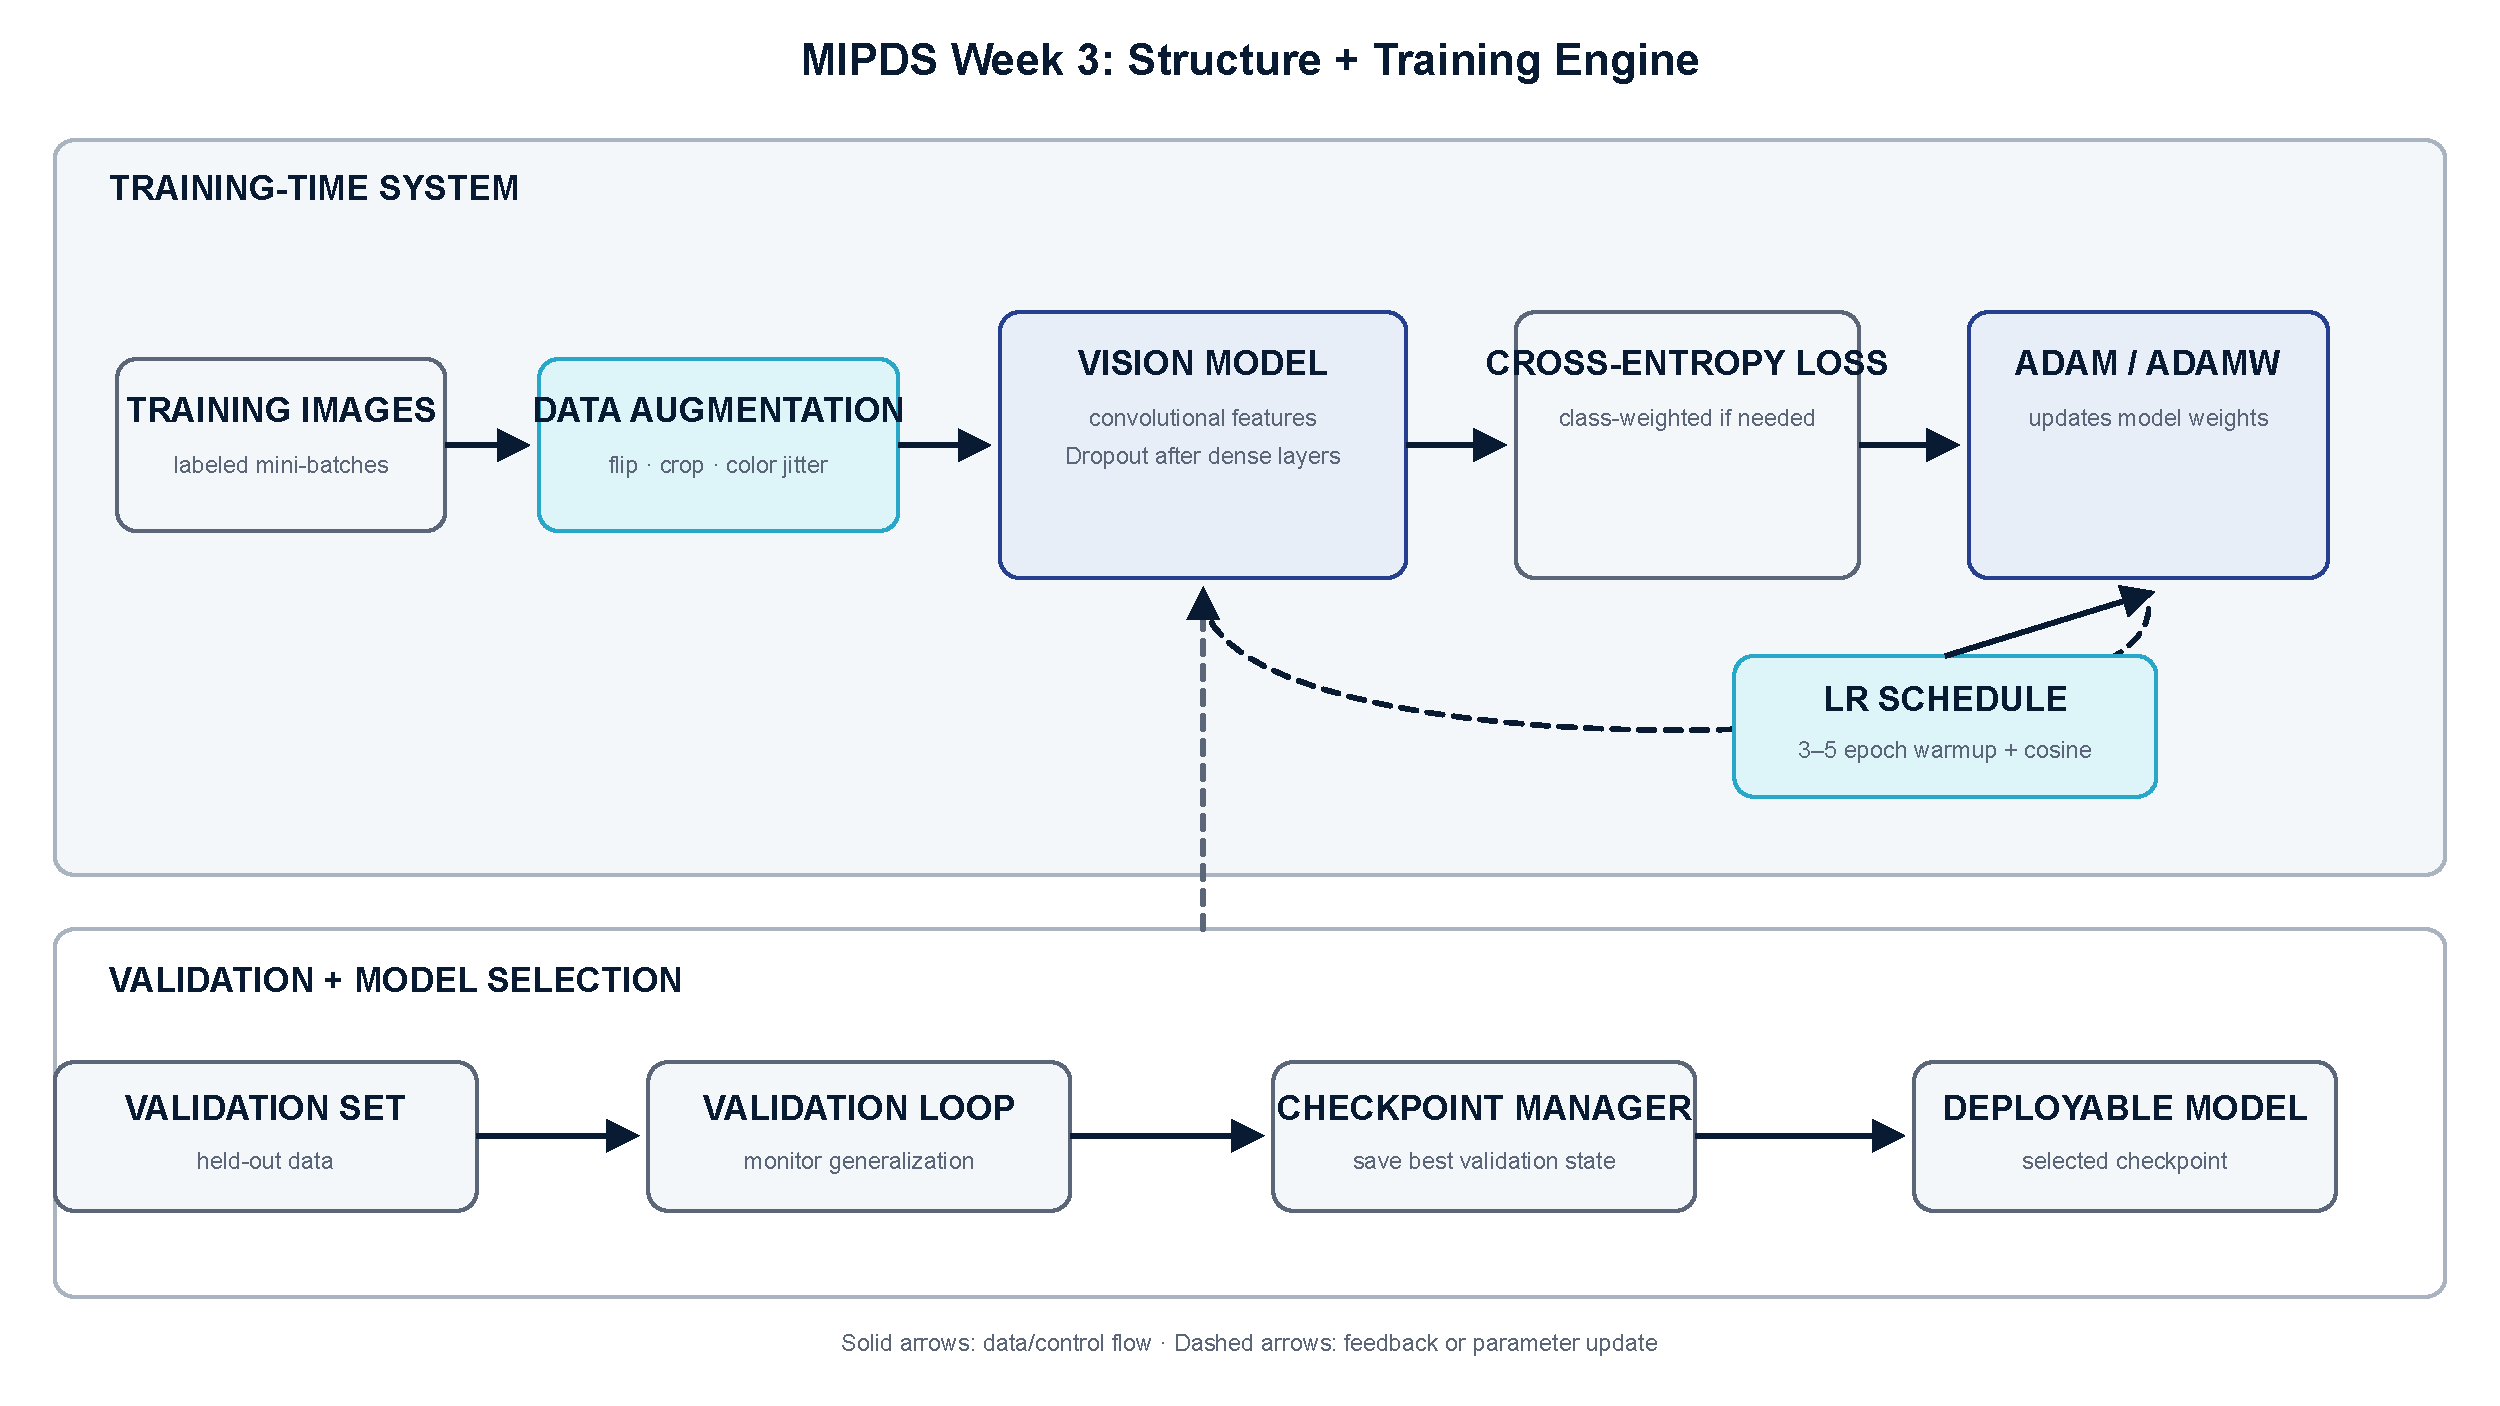
\includegraphics[width=\linewidth,height=.72\textheight,keepaspectratio]{chapters/../assets/figures/fig-3-10-mipds-training-engine.pdf}
\caption*{\textbf{Figure 3.10:} MIPDS Week 3: Structure + Training Engine.
\emph{Every labeled component in this diagram corresponds to a concept
from this chapter. You should be able to explain each one, justify its
presence, and describe what failure mode it prevents.}}
\addcontentsline{lof}{figure}{\protect\numberline{3.10}MIPDS Week 3: Structure + Training Engine. Every labeled component in this diagram corresponds to a concept from this chapter. You should be able to explain each one, justify its presence, and describe what failure mode it prevents.}
\label{figure-3-10}
\end{figure}
\FloatBarrier

\subsection{Designing the Training Engine: Key
Decisions}\label{designing-the-training-engine-key-decisions}

\subsection{Loss Function}\label{loss-function}

The immediate task for the MIPDS vision module is multi-class
classification: identifying what objects or scenes are present in an
image. Cross-entropy loss is the appropriate choice. If your initial
dataset has significant class imbalance --- which is common in
real-world data --- class-weighted cross-entropy should be considered
from the outset, not retrofitted after you observe poor performance on
minority classes.

Looking ahead: as MIPDS grows to include image segmentation capabilities
(for precise object localization), the loss will need to expand to
include Dice or IoU loss. And when the multimodal alignment module is
added in Week 10, contrastive loss will become relevant. Designing your
training infrastructure to be modular --- so that loss functions can be
composed without rebuilding the training loop --- is good forward
planning.

\subsection{Optimizer and Learning
Rate}\label{optimizer-and-learning-rate}

Adam (or AdamW) is the recommended starting optimizer for MIPDS. It
requires minimal tuning, converges reliably, and is robust to the
learning rate choices made by new practitioners. For your initial
experiments, a learning rate of 3e-4 to 1e-3 is a reasonable starting
range.

For the learning rate schedule, a warmup period of 3--5 epochs followed
by cosine annealing is recommended. This two-part schedule will serve
you throughout the course: the warmup prevents early instability, and
cosine annealing provides graceful convergence. When you add Transformer
components in Week 8, you will find that this exact schedule is standard
practice for large language models --- designing it well now pays
dividends later.

\subsection{Regularization Plan}\label{regularization-plan}

Apply Dropout with a rate of 0.3--0.5 after the dense layers (not after
the convolutional layers --- convolutional features should be allowed to
develop fully before regularization). Apply L2 weight decay through
AdamW rather than implementing it separately. Apply standard data
augmentation: horizontal flips, random crops, and moderate color jitter.
This combination is conservative and broadly effective; if validation
performance reveals persistent overfitting, increase Dropout rate before
increasing L2.

\subsection{Validation Protocol}\label{validation-protocol}

Reserve 15\% of your dataset as a validation set, split before any
preprocessing decisions are made. Monitor validation loss after every
epoch. Set early stopping patience to 10 epochs --- meaning training
continues for up to 10 epochs after the best validation loss, in case
the model is still in a temporary plateau rather than a permanent one.
Save a checkpoint at every epoch; deploy the checkpoint with the best
validation loss.

\begin{longtable}[]{@{}
  >{\raggedright\arraybackslash}p{(\linewidth - 0\tabcolsep) * \real{1.0016}}@{}}
\toprule\noalign{}
\endhead
\bottomrule\noalign{}
\endlastfoot
\textbf{⚖️ An Ethical Checkpoint} \textbar{}

Before finalizing your training setup, ask: what does my validation set
actually represent? If your training data came from one demographic,
hospital, geography, or camera type, your validation set --- drawn from
the same distribution --- may look artificially good. A model that
generalizes well within a population may fail badly when deployed beyond
it. The training loop has no mechanism to detect this kind of
distributional shift. It is a design-time responsibility, not a
training-time one. The most important question you can ask about your
validation set is: is it representative of the world the model will be
deployed in? \\
\end{longtable}

\addcontentsline{toc}{section}{Hands-On Exploration}
\begin{DLSectionPanel}{HANDS-ON EXPLORATION}

\subsection{Seeing Training Dynamics in
Action}\label{seeing-training-dynamics-in-action}

This activity is designed to build intuition through observation. You
will not write a network from scratch. Instead, you will change a small
number of training parameters and carefully observe the effect on
learning curves. The goal is to develop a personal vocabulary for
reading training behavior --- the same way a doctor learns to read vital
signs, not by memorizing what each pattern means, but by observing them
in context until recognition becomes instinctive.

\begin{longtable}[]{@{}
  >{\raggedright\arraybackslash}p{(\linewidth - 0\tabcolsep) * \real{1.0036}}@{}}
\toprule\noalign{}
\endhead
\bottomrule\noalign{}
\endlastfoot
\textbf{🛠️ Setup} \textbar{}

Platform: Google Colab (free tier is sufficient). A starter notebook is
provided that trains a small CNN on CIFAR-10 --- 50,000 images across 10
classes. The architecture is fixed and provided. All you need to change
are the training configuration parameters identified below.

Estimated time: 45--60 minutes. Each experiment takes 5--8 minutes to
run. Read the prompts before running --- knowing what to look for before
the curve appears is part of the skill. \\
\end{longtable}

\subsection{Experiment 1: Establish a
Baseline}\label{experiment-1-establish-a-baseline}

Run the default configuration: Adam optimizer, learning rate 0.001, no
Dropout, no data augmentation, 25 epochs.

Record and reflect:

\begin{itemize}
\item
  At what epoch do training and validation accuracy visibly diverge?
\item
  What is the approximate final gap between training accuracy and
  validation accuracy?
\item
  Does validation accuracy appear to be still improving at epoch 25, or
  has it plateaued?
\item
  What word would you use to describe this model\textquotesingle s
  training state --- overfitting, underfitting, or well-fit?
\end{itemize}

\subsection{Experiment 2: Activate
Regularization}\label{experiment-2-activate-regularization}

Enable Dropout (rate=0.4) and data augmentation (horizontal flip +
random crop). Keep all other settings identical to Experiment 1.

Observe the change:

\begin{itemize}
\item
  Training accuracy is almost certainly lower than in Experiment 1. Why?
  What does this tell you about what Dropout is doing?
\item
  Is validation accuracy higher or lower than in Experiment 1? By how
  much?
\item
  Has the training-validation gap changed? What does this tell you about
  generalization?
\item
  Write one sentence describing what regularization did to this
  model\textquotesingle s behavior, in plain language.
\end{itemize}

\subsection{Experiment 3: Learning Rate Stress
Test}\label{experiment-3-learning-rate-stress-test}

Return to the Experiment 1 configuration. Now run two additional
training runs: one with learning rate 0.01 (10× higher), and one with
learning rate 0.1 (100× higher).

For each:

\begin{itemize}
\item
  Describe what the training loss curve looks like in the first 5
  epochs. Is it descending smoothly? Erratically? Not at all?
\item
  Does the training run succeed (produce a model significantly better
  than chance) or fail?
\item
  Sketch a description of what you would expect the curve to look like
  at 0.0001 (100× lower than baseline), without running it --- based on
  the pattern you have observed.
\end{itemize}

\subsection{Write-Up}\label{write-up}

In 400--600 words, describe what you observed across all three
experiments. Use the vocabulary from this chapter --- overfitting,
validation loss, learning rate, regularization, generalization gap ---
but write in your own voice, describing what you actually saw and what
you think it means. Attach your three learning curve images. There are
no wrong answers; the quality of reasoning matters more than the
specific numbers.

\end{DLSectionPanel}

\section{Case Study}\label{case-study-1}

\subsection{CheXNet: When Training Decisions Saved Lives --- and
Concealed
Limits}\label{chexnet-when-training-decisions-saved-lives-and-concealed-limits}

\subsection{The Problem}\label{the-problem-1}

Pneumonia kills more than 2.5 million people per year globally, the
majority in low-income settings where access to experienced radiologists
is scarce. Even in well-resourced hospitals, radiology departments are
chronically understaffed, and chest X-ray backlogs mean patients wait
hours or days for interpretations that could guide urgent treatment. The
question driving the CheXNet project at Stanford in 2017 was simple and
audacious: could a deep learning model read chest X-rays at the level of
a practicing radiologist?

\subsection{The Architecture}\label{the-architecture}

CheXNet was built on DenseNet-121, a convolutional architecture that we
will study in depth in Week 5. It processed chest X-rays as images and
produced probability scores for 14 different thoracic conditions ---
pneumonia, atelectasis, effusion, and eleven others --- simultaneously.
The architecture itself was not novel for 2017. What distinguished
CheXNet was a series of training decisions, each directly illustrating
principles from this chapter.

\subsection{Training Decision 1: Transfer Learning as
Initialization}\label{training-decision-1-transfer-learning-as-initialization}

CheXNet began its training not with random weights but with weights
pretrained on ImageNet --- a dataset of over a million natural
photographs: cats, cars, fire hydrants, grocery items. At first glance,
this seems strange. What does a fire hydrant have to do with a pneumonia
lesion?

But consider what the early layers of an ImageNet-trained network have
learned: edges, textures, gradients, local patterns of light and dark.
These low-level features are not specific to photographs of consumer
goods. They are present in chest X-rays as well --- the gradual density
transitions at a lung boundary, the sharp edge of a rib, the subtle
texture difference between healthy and consolidating tissue.
Initializing with ImageNet weights gave the network a rich vocabulary of
low-level visual features, rather than starting from the random babbling
of random initialization. Training from the pretrained initialization
required far fewer epochs and produced substantially better performance
than training from scratch on the medical dataset alone.

This is the principle of transfer learning: weights learned for one task
often provide a productive starting point for a related task. It is one
of the most important practical tools in modern deep learning, and we
will explore it systematically in later weeks.

\subsection{Training Decision 2: Class-Weighted Loss for Imbalanced
Data}\label{training-decision-2-class-weighted-loss-for-imbalanced-data}

The NIH ChestX-ray14 dataset contains over 112,000 images. Of these,
fewer than 2\% are labeled positive for pneumonia. A naive model trained
with standard cross-entropy loss quickly discovers the path of least
resistance: predict "no pneumonia" for almost every image. This strategy
achieves 98\% accuracy while being completely useless as a clinical
tool.

The CheXNet team addressed this through class-weighted loss: the
contribution of positive (pneumonia) examples to the total loss was
multiplied by a factor inversely proportional to their frequency. Each
pneumonia image contributed 50 times more to the loss than each
non-pneumonia image, forcing the model to attend to the rare positive
cases rather than ignoring them to achieve high average accuracy.

This choice is a microcosm of the ethical dimension of loss function
design. Unweighted loss, in this context, does not mean neutral --- it
means the interests of the majority class dominate. Weighting the loss
is not a technical bias correction; it is an explicit value statement:
misclassifying a sick patient is far more costly than misclassifying a
healthy one.

\subsection{Training Decision 3: Data Augmentation for Distribution
Robustness}\label{training-decision-3-data-augmentation-for-distribution-robustness}

Chest X-ray images vary enormously in the real world: different
radiography equipment produces different image characteristics;
different technicians position patients differently; different
institutions use different imaging protocols. A model trained on images
from one institution may fail at another because the image statistics
shift in ways that the model, trained only on one distribution, cannot
handle.

The team applied horizontal flipping, random rotation within ±10
degrees, and brightness and contrast perturbation during training. These
augmentations simulated the kind of variation the model would encounter
in deployment. Horizontal flipping is noteworthy: in most medical
contexts, it would be anatomically incorrect (a mirrored lung is
pathologically significant). The team used it anyway, reasoning that the
augmentation benefit outweighed the anatomical inconsistency for the
pneumonia detection task. This is the kind of domain-specific judgment
that augmentation strategies require.

\subsection{The Results --- and Their
Limits}\label{the-results-and-their-limits}

CheXNet achieved a ROC-AUC of 0.768 on pneumonia detection in the
validation set, compared to a mean of 0.633 for four radiologists
evaluated on the same subset of 420 images. The result was extraordinary
by the metrics used --- and was heavily publicized as evidence that AI
could outperform physicians in radiology.

But honest evaluation reveals important limitations that training
metrics alone cannot capture:

\begin{itemize}
\item
  The radiologist comparison used only 420 images --- a tiny subset
  evaluated under unusual, time-pressured conditions. Subsequent studies
  found inconsistent results when the comparison was replicated under
  more realistic conditions.
\item
  All 112,000 training images came from a single institution --- the
  National Institutes of Health. Models trained on single-site data
  routinely fail to generalize to other hospital systems, where imaging
  equipment, patient demographics, and annotation practices differ. This
  is distribution shift, and it cannot be corrected by better training
  without more diverse data.
\item
  The labels were extracted from radiology reports using natural
  language processing, not verified by radiologists reviewing each
  image. A significant fraction of labels may be incorrect. The model
  learned from imperfect supervision --- common in practice, and
  honestly important to acknowledge.
\item
  Performance varied substantially across the 14 diseases --- strong on
  some conditions, weak on others. Aggregate metrics like AUC can mask
  failures on specific, important categories.
\end{itemize}

\begin{longtable}[]{@{}
  >{\raggedright\arraybackslash}p{(\linewidth - 0\tabcolsep) * \real{1.0024}}@{}}
\toprule\noalign{}
\endhead
\bottomrule\noalign{}
\endlastfoot
\textbf{📌 What CheXNet Teaches Us About Training}

CheXNet is not primarily a story about a brilliant architecture. It is a
story about training choices: which loss function captures what
clinicians care about; how initialization enables learning from limited
data; how augmentation builds robustness to real-world variation. Each
of these decisions was grounded in the principles this chapter covers.
Each could have been made differently --- with different consequences.

It is also a story about the limits of metrics. High validation
performance does not guarantee real-world utility. The gap between what
a loss function measures and what a deployment context requires is a
persistent challenge in applied machine learning --- and bridging it
requires both technical rigor and genuine engagement with the users and
contexts the system is designed to serve. \\
\end{longtable}

\addcontentsline{toc}{section}{Chapter Summary}
\begin{DLSectionPanel}{CHAPTER SUMMARY}

\subsection{What We Have Learned}\label{what-we-have-learned-1}

This chapter crossed the threshold between architecture and
intelligence. The network you designed in Chapter 2 had structure,
organization, and theoretical capacity. What it lacked was experience
--- the millions of small adjustments that convert a randomly
initialized weight matrix into a system that can genuinely perceive and
understand.

We began with the loss function --- not as a technical formality but as
a value system. The loss function formally specifies what the model
considers success. Choosing it carelessly produces systems that optimize
beautifully for the wrong objective. We studied the two most important
loss functions --- MSE for regression, cross-entropy for classification
--- and explored the specialized forms that more complex tasks require.
The Nairobi hospital story, which opened this chapter, was always a
story about this: a loss function designed without consideration of
clinical priorities produced a model that learned to be confidently
blind.

From loss, we moved to optimization. Gradient descent is the
navigational strategy: given a loss landscape, follow the downhill
direction, one small step at a time. The learning rate determines step
size --- too large and we overshoot, too small and we never arrive.
Backpropagation is the efficient algorithm that computes, in a single
backward pass, how much every weight in the network contributed to the
current error. Modern optimizers like Adam and SGD with momentum extend
gradient descent with adaptive mechanisms that make training more
reliable across a wider range of problems.

We studied the training loop --- the four-phase rhythm of forward pass,
loss computation, backward pass, and parameter update that repeats,
epoch after epoch, until the network has learned what we want it to
know. We introduced learning rate schedules as a way to adjust ambition
over time, and checkpointing as a way to preserve the best version of a
training run.

We then confronted the central challenge of training: generalization. A
model that memorizes training data is not intelligent --- it is a
sophisticated lookup table. Overfitting is the pathology; Dropout, L2
regularization, data augmentation, and early stopping are the
treatments, each grounded in a clear conceptual motivation rather than
arbitrary configuration choices. We saw that underfitting is the
opposite problem, less dramatic but equally real, requiring opposite
interventions.

We learned to read learning curves as diagnostic instruments, and to
recognize the gradient pathologies --- vanishing gradients and exploding
gradients --- that can silently undermine training in deep networks. And
through the CheXNet case study, we saw all of these principles operating
together in a real system, including the honest acknowledgment of where
training metrics diverge from deployment realities.

Finally, you applied these principles to MIPDS: designing the training
engine for the vision component, making principled decisions about loss
function, optimizer, regularization strategy, and validation protocol.
Structure has met learning. The system has begun to become real.

\begin{longtable}[]{@{}
  >{\raggedright\arraybackslash}p{(\linewidth - 0\tabcolsep) * \real{1.0014}}@{}}
\toprule\noalign{}
\endhead
\bottomrule\noalign{}
\endlastfoot
\textbf{🔭 Looking Ahead: Chapter 4}

In the next chapter, we return to architecture --- but now as
practitioners who understand training. We will study the great CNN
architectures of the modern era: VGG, ResNet, Inception, DenseNet. We
will see that residual connections were not just an architectural
innovation --- they were a training innovation, specifically designed to
solve the vanishing gradient problem we encountered in Section 5 of this
chapter. Batch Normalization, which we introduced briefly here as a
training stabilizer, will emerge as a structural component that changed
what architectures could be built. The training principles of Chapter 3
are not behind us; they are the foundation on which every architectural
advance in Chapter 4 was built. \\
\end{longtable}

\end{DLSectionPanel}

\addcontentsline{toc}{section}{Review Questions}
\begin{DLSectionPanel}{REVIEW QUESTIONS}

The questions below are designed for discussion and debate, not for
definitive answers. Strong responses will acknowledge multiple
perspectives, engage with complexity, and draw on specific concepts from
the chapter. Consider them as starting points, not endpoints.

\subsection{1. The Loss Function as
Ethics}\label{the-loss-function-as-ethics}

The loss function formally specifies what a model considers success. In
the Nairobi hospital scenario, unweighted cross-entropy on an imbalanced
dataset taught the model that missing pneumonia was acceptable.
Class-weighted loss changed what the model valued. If loss functions
are, in effect, value systems encoded in mathematics, who should design
them --- engineers, clinicians, patients, regulators, or some
combination? Can technical expertise substitute for stakeholder input in
making these choices? What structures would help ensure that loss
function design reflects the priorities of the people affected by the
system?

\subsection{2. Generalization and the Limits of
Validation}\label{generalization-and-the-limits-of-validation}

CheXNet achieved strong performance on a validation set drawn from the
same hospital that produced the training data. When deployed at other
institutions, performance varied. The validation set gave an honest
signal about generalization within the training distribution, but not
about generalization across distributions. Is this a problem with the
training process, or with how validation sets are designed? What would a
validation protocol look like that actually measured the kind of
generalization that matters for deployment? Is such a protocol even
achievable without testing in the real world?

\subsection{3. Occam\textquotesingle s Razor and Model
Simplicity}\label{occams-razor-and-model-simplicity}

L2 regularization encodes a preference for simple models with small
weights. This preference is philosophically motivated --- simpler
explanations generalize better --- but it is also an assumption. Are
there domains where complex, high-weight solutions are genuinely
optimal? What happens when the signal in the training data is subtle and
irregular, and the simple solution genuinely misses something important?
Does the preference for simplicity encode any deeper epistemological
commitment --- and is that commitment always warranted?

\subsection{4. The Overfitting Economy}\label{the-overfitting-economy}

Overfitting --- the memorization of training specifics at the expense of
general patterns --- is presented here as a technical failure mode in
neural networks. But consider whether the same pattern appears in human
organizations. An executive team that optimizes for quarterly metrics
may be "overfitting" to a short-term evaluation signal at the expense of
long-term resilience. A teacher who teaches to the test may be producing
students who have overfit the exam. What does this analogy illuminate
about the technical problem? And what does it obscure?

\subsection{5. Transfer Learning and Borrowed
Understanding}\label{transfer-learning-and-borrowed-understanding}

CheXNet started from ImageNet weights --- features learned from
photographs of consumer goods --- and used them as the foundation for
detecting disease in chest X-rays. Does a model that begins its
understanding of medical images by looking at fire hydrants and food
items have something meaningfully in common with a radiologist who
learned to read X-rays by studying anatomy? Or is "transfer learning" a
purely statistical phenomenon with no deeper cognitive significance?
Does your answer change depending on what question you are asking the
system to answer?

\subsection{6. Learning Rate and
Patience}\label{learning-rate-and-patience}

Learning rate warmup --- starting training very slowly and gradually
accelerating --- is a training technique with a striking pedagogical
analogy: we often introduce new students to ideas gently, at low
intensity, before demanding rigorous application. Yet warmup in neural
networks is motivated by numerical stability, not by any theory of
learning readiness. Is this analogy genuinely illuminating, or does it
mislead us about how neural networks learn? Are there aspects of human
learning that have no neural network equivalent, and vice versa?

\subsection{7. The Debugging Mindset}\label{the-debugging-mindset}

Debugging a training failure requires systematic reasoning under
uncertainty: forming hypotheses, designing experiments, interpreting
ambiguous evidence. This is fundamentally the same skill as medical
diagnosis, engineering troubleshooting, or scientific investigation. Yet
it is rarely taught explicitly in technical curricula --- students are
usually given architectures that work, datasets that are clean, and loss
functions that are standard. What are the costs of not teaching
debugging as a first-class skill? How would you design a course --- or
this course --- to build genuine debugging fluency in students?

\subsection{8. Ethical Responsibility in Training
Pipelines}\label{ethical-responsibility-in-training-pipelines}

When a deployed AI system causes harm --- a medical AI that misses a
diagnosis, a hiring algorithm that discriminates, a content moderation
system that suppresses legitimate speech --- responsibility is typically
distributed across many people: those who collected the training data,
those who designed the loss function, those who configured the training
pipeline, those who validated the model, and those who deployed it. Does
this distribution of responsibility make accountability harder to
assign? Is diffused responsibility a feature or a bug of complex
sociotechnical systems? What institutional structures might help?

\end{DLSectionPanel}

\addcontentsline{toc}{section}{Further Reading}
\begin{DLSectionPanel}{FURTHER READING}

\subsection{On Optimization and Training
Fundamentals}\label{on-optimization-and-training-fundamentals}

\begin{itemize}
\item
  Goodfellow, I., Bengio, Y., \& Courville, A. (2016). Deep Learning.
  MIT Press. Chapter 8 (Optimization for Training Deep Models) is the
  definitive technical treatment of gradient descent and its variants.
  Available free at deeplearningbook.org.
\item
  Ruder, S. (2016). An overview of gradient descent optimization
  algorithms. arXiv:1609.04747. An accessible survey of modern
  optimizers, clearly explaining Adam, RMSprop, Adagrad, and their
  relationships.
\item
  Smith, L. N. (2017). Cyclical learning rates for training neural
  networks. IEEE Winter Conference on Applications of Computer Vision.
  The paper that popularized learning rate range tests and cyclical
  schedules --- practical tools every practitioner should know.
\end{itemize}

\subsection{On Regularization and
Generalization}\label{on-regularization-and-generalization}

\begin{itemize}
\item
  Srivastava, N., Hinton, G., Krizhevsky, A., Sutskever, I., \&
  Salakhutdinov, R. (2014). Dropout: A simple way to prevent neural
  networks from overfitting. Journal of Machine Learning Research, 15,
  1929--1958. The original Dropout paper --- readable and foundational.
\item
  Zhang, C., Bengio, S., Hardt, M., Recht, B., \& Vinyals, O. (2017).
  Understanding deep learning requires rethinking generalization. ICLR.
  A surprising and important paper demonstrating that deep networks can
  memorize random labels --- prompting a rethinking of what
  regularization actually does.
\item
  Loshchilov, I., \& Hutter, F. (2019). Decoupled weight decay
  regularization. ICLR. The paper introducing AdamW --- essential
  reading if you use Adam in practice.
\end{itemize}

\subsection{On the Historical Significance of Training
Advances}\label{on-the-historical-significance-of-training-advances}

\begin{itemize}
\item
  Glorot, X., \& Bengio, Y. (2010). Understanding the difficulty of
  training deep feedforward neural networks. AISTATS. The paper that
  identified the vanishing gradient problem precisely and introduced
  careful weight initialization as a solution.
\item
  Ioffe, S., \& Szegedy, C. (2015). Batch normalization: Accelerating
  deep network training by reducing internal covariate shift. ICML.
  Batch Normalization changed what deep networks could be trained ---
  foundational for every modern architecture.
\end{itemize}

\subsection{On the CheXNet Case Study}\label{on-the-chexnet-case-study}

\begin{itemize}
\item
  Rajpurkar, P., Irvin, J., Ball, R. L., Zhu, K., Yang, B., Mehta, H.,
  ... \& Ng, A. Y. (2017). CheXNet: Radiologist-level pneumonia
  detection on chest X-rays with deep learning. arXiv:1711.05225. The
  original paper, clearly written and accessible.
\item
  Oakden-Rayner, L. (2018). CheXNet: An in-depth review. Blog post at
  lukeoakdenrayner.wordpress.com. A careful and important critical
  analysis of the CheXNet claims --- essential reading for understanding
  the gap between benchmark performance and clinical utility.
\end{itemize}

\subsection{On Ethics and Societal
Impact}\label{on-ethics-and-societal-impact}

\begin{itemize}
\item
  Obermeyer, Z., Powers, B., Vogeli, C., \& Mullainathan, S. (2019).
  Dissecting racial bias in an algorithm used to manage the health of
  populations. Science, 366(6464), 447--453. A landmark study showing
  how an apparently neutral loss function (cost of care, as a proxy for
  need) embedded systematic racial bias.
\item
  Caruana, R., Lou, Y., Gehrke, J., Koch, P., Sturm, M., \& Elhadad, N.
  (2015). Intelligible models for healthcare: Predicting pneumonia risk
  and hospital 30-day readmission. Proceedings of KDD. A sobering case
  study in which a complex model learned that asthma was protective
  against pneumonia mortality --- because asthmatic patients received
  more aggressive care.
\end{itemize}

\subsection{Interactive Tools}\label{interactive-tools}

\begin{itemize}
\item
  TensorFlow Playground (https://playground.tensorflow.org) --- Visual
  neural network exploration. Particularly useful for building intuition
  about overfitting, regularization, and the effect of learning rate.
\item
  Weights \& Biases (https://wandb.ai) --- Professional experiment
  tracking and visualization. Free for academic use. The
  industry-standard tool for monitoring training runs and comparing
  experiments.
\item
  fast.ai Practical Deep Learning for Coders (https://course.fast.ai)
  --- A practice-first deep learning course whose training section is
  particularly strong on learning rate finding, warmup schedules, and
  transfer learning.
\end{itemize}

⬡ ⬡ ⬡

\emph{End of Chapter 3 --- Second Edition}

\part{Vision Systems}

Part II

Vision systems transform spatial structure into increasingly abstract
feature maps, predictions, and decisions.

Building on the training foundations of Part I, this Part examines how
architecture encodes assumptions about images. Chapter 4 follows the
development of modern convolutional networks, residual learning,
efficient scaling, transfer learning, and Vision Transformers. Chapter 5
moves beyond classification to object detection and segmentation, where
a model must preserve spatial information rather than produce only a
label. Chapter 6 completes the vision pipeline through evaluation, error
analysis, dataset discipline, representation inspection, experiment
tracking, and auditing.

The transition is from training a model to engineering a defensible
visual system. Readers learn to connect feature hierarchy and spatial
structure with task requirements, evaluation design, and deployment
constraints.

\end{DLSectionPanel}

\DLChapterOpener{Vision Systems}{The Architecture of Sight}{How Researchers Redesigned the CNN—and What They Built Instead}{\item \textbf{Explain the degradation problem} in deep convolutional networks
--- what it is, why it happens, and why it is distinct from the
vanishing gradient problem explored in Chapter 3.
\item \textbf{Describe residual connections} and explain, both intuitively and
mathematically, why learning the residual \(F(x) = H(x) - x\) stabilizes
training in very deep networks.
\item \textbf{Explain the design logic of Inception modules}, including the
role of parallel multi-scale processing and the dimensionality-reducing
1×1 convolution.
\item \textbf{Describe EfficientNet\textquotesingle s compound scaling
principle} --- why coordinated scaling of depth, width, and resolution
outperforms scaling any single dimension independently.
\item \textbf{Explain how Vision Transformers process images}, from patch
embedding through positional encoding and self-attention, and articulate
the tradeoffs between CNN and Transformer-based vision.
\item \textbf{Select an appropriate architecture} given a specific combination
of task complexity, dataset size, and resource constraint --- and
justify that selection with principled reasoning.
\item \textbf{Apply transfer learning} by loading a pre-trained backbone and
adapting it to a new classification task, understanding which layers to
freeze and when to unfreeze them.
\item \textbf{Reason about the ethical dimensions} of architecture selection
--- including how model efficiency, compute access, and deployment
context intersect with equity of access and real-world impact.}

How Researchers Redesigned the CNN---and What They Built Instead

\hfill\break

\section{Opening Narrative}\label{opening-narrative-2}

\subsection{The Day Deeper Got Worse}\label{the-day-deeper-got-worse}

In the spring of 2015, a team of researchers at Microsoft Research Asia
ran an experiment that should not have produced the results it did.

They were studying convolutional neural networks --- the architecture
that had dominated image recognition since AlexNet\textquotesingle s
landmark 2012 victory, which we encountered in Chapter 2. The hypothesis
was reasonable, almost obvious: if deeper networks learn more complex
features, then a 56-layer network should outperform a 20-layer network
on the same image classification task. More layers meant more
representational power. More power meant better performance. This was
the received wisdom of the field.

What Kaiming He and his colleagues found instead stopped them cold.

The 56-layer network was \emph{worse}. Not just slightly worse ---
measurably, consistently worse, on both the training data and the test
data. And this was the strange part: it was not the kind of failure that
comes from overfitting, where a model memorizes training examples and
performs poorly on new ones. Both training error and test error were
higher for the deeper network. Something fundamental was going wrong
during the learning process itself. Adding more capacity was making the
network \emph{less} capable.

He\textquotesingle s team called this the \textbf{degradation problem},
and it was genuinely puzzling. In theory, a deeper network should be
able to solve any problem that a shallower one can --- after all, the
deeper network could simply learn to ignore its extra layers, setting
their weights so they act as identity functions that pass their input
straight through. But in practice, the optimization process --- the
gradient descent and backpropagation machinery we explored in Chapter 3
--- could not find that solution. The extra layers were not being
ignored; they were distorting the signal.

The insight that resolved this came from a deceptively simple question:
what if, instead of asking each layer to learn the full transformation
from its input to its output, we asked it to learn only the
\emph{correction} --- the difference between where the network currently
is and where it needs to be?

The fix was a small architectural change. Before the output of a block
of layers is computed, add a shortcut that bypasses those layers
entirely and adds the original input directly to their output. Now each
block does not have to learn an arbitrary mapping \(H(x)\). It only has
to learn the residual \(F(x) = H(x) - x\) --- the adjustment on top of
what was already there. If the optimal adjustment is zero, the block can
simply learn to output zeros, and the identity shortcut carries the
input forward unchanged. Gradient descent has no trouble finding this
solution.

The result --- published as "Deep Residual Learning for Image
Recognition" --- won the 2015 ImageNet competition, the COCO detection
competition, the COCO segmentation competition, and the ImageNet
localization competition simultaneously. The winning network had 152
layers. Two years earlier, that depth would have been inconceivable.

This is the story of this chapter: not just the architectures that
emerged after the basic CNN, but the \emph{problems} that forced their
invention. Every design we will study this week is an answer to a
specific question. What are those questions? Why did the answers take
the forms they did? And when you face a new problem, which answer should
you reach for?

By the end of this chapter, you will be able to answer all three.

\section{Key Terms and Concepts}\label{key-terms-and-concepts-3}

\begin{longtable}[]{@{}
  >{\raggedright\arraybackslash}p{(\linewidth - 2\tabcolsep) * \real{0.1089}}
  >{\raggedright\arraybackslash}p{(\linewidth - 2\tabcolsep) * \real{0.8861}}@{}}
\toprule\noalign{}
\begin{minipage}[b]{\linewidth}\raggedright
\textbf{Term}
\end{minipage} & \begin{minipage}[b]{\linewidth}\raggedright
\textbf{Plain-Language Definition}
\end{minipage} \\
\midrule\noalign{}
\endhead
\bottomrule\noalign{}
\endlastfoot
\textbf{Degradation Problem} & The counterintuitive failure mode in
which adding more layers to a plain deep network makes performance
\emph{worse} --- not because of overfitting, but because the
optimization process cannot effectively navigate the deeper loss
landscape. \\
\textbf{Residual Connection (Skip Connection)} & A shortcut pathway in a
neural network that adds a layer\textquotesingle s input directly to its
output, bypassing the layer\textquotesingle s learned transformation.
This allows the network to learn corrections on top of what already
exists, rather than learning full transformations from scratch. \\
\textbf{Residual Block} & A standard building block of ResNets. Contains
two or more convolutional layers plus a skip connection from input to
output. The output is \(F(x)\) + x, where \(F(x)\) is what the layers
learned and x is the original input. \\
\textbf{Bottleneck Block} & A three-layer variant of the residual block
(1×1 → 3×3 → 1×1 convolutions) used in deeper ResNets to reduce
computational cost while preserving representational capacity. The 1×1
layers compress and then restore the channel dimension around the
expensive 3×3 convolution. \\
\textbf{Inception Module} & A building block that applies multiple
convolutional filters of different sizes (1×1, 3×3, 5×5) in parallel to
the same input and concatenates their outputs. Allows the network to
simultaneously detect features at multiple scales without committing to
a single filter size. \\
\textbf{Compound Scaling} & EfficientNet\textquotesingle s method for
scaling neural networks by jointly increasing depth (more layers), width
(more channels), and input resolution --- using a fixed compound
coefficient --- rather than scaling any single dimension in
isolation. \\
\textbf{Depthwise Separable Convolution} & A factorized alternative to
standard convolution that separates spatial filtering (applied
independently to each input channel) from channel mixing (a 1×1
convolution across channels). Dramatically reduces computation while
preserving expressive power. \\
\textbf{Vision Transformer (ViT)} & An architecture that processes
images by dividing them into fixed-size patches, treating each patch as
a token (similar to a word in a sentence), and applying a standard
Transformer encoder with self-attention to model relationships between
patches. \\
\textbf{Patch Embedding} & The first step in a Vision Transformer: each
image patch is flattened into a vector and linearly projected into a
lower-dimensional embedding space, preparing it for Transformer
processing. \\
\textbf{Positional Encoding} & Information added to patch embeddings to
indicate each patch\textquotesingle s location in the image. Necessary
because self-attention, unlike convolution, has no built-in notion of
spatial position. \\
\textbf{Self-Attention} & A mechanism that allows each element in a
sequence to attend to --- and be influenced by --- every other element
simultaneously. In Vision Transformers, this gives every image patch a
global view of the entire image from the very first layer. \\
\textbf{Transfer Learning} & The practice of using weights learned on a
large source task (typically ImageNet classification) as the starting
point for a new, smaller task. The lower-level features learned ---
edges, textures, shapes --- are genuinely transferable across visual
domains. \\
\textbf{Feature Extraction} & Using the early and middle layers of a
pre-trained network as a fixed feature computer. The
backbone\textquotesingle s weights are frozen; only a new classification
head placed on top is trained. \\
\textbf{Fine-Tuning} & A second stage of transfer learning in which some
or all of the backbone\textquotesingle s weights --- initially frozen
--- are unfrozen and allowed to adjust with a very low learning rate,
adapting to the specifics of the new task. \\
\textbf{Global Average Pooling} & An operation applied before the
classification head that reduces each feature map to a single number by
averaging all its spatial values. Produces a compact feature vector
while reducing the number of parameters compared to fully-connected
layers. \\
\textbf{Batch Normalization} & A technique that normalizes the
activations within each layer during training, keeping them in a stable
range. Enables faster training, supports higher learning rates, and acts
as a mild regularizer --- introduced in Chapter 3 and used heavily in
the architectures here. \\
\textbf{Feature Pyramid} & A hierarchical multi-scale representation in
which the same backbone is used to extract features at multiple spatial
resolutions simultaneously, enabling detection of objects of different
sizes. \\
\textbf{Knowledge Distillation} & A compression technique in which a
smaller "student" network is trained to mimic the output behavior of a
larger, more accurate "teacher" network, transferring the
teacher\textquotesingle s learned knowledge into a more deployable
form. \\
\textbf{Model Compression} & A family of techniques --- including
pruning (removing unnecessary weights), quantization (reducing numerical
precision), and distillation --- aimed at reducing a
model\textquotesingle s size and computational cost while minimizing
accuracy loss. \\
\textbf{Multi-Head Attention} & The version of self-attention used in
practice: the attention computation is split into multiple independent
"heads," each attending to different aspects of the input. The outputs
are concatenated and projected. In Vision Transformers, this allows each
patch to simultaneously attend to nearby patches, distant patches, and
patches with similar content. \\
\end{longtable}

\section{Why Depth Alone Isn\textquotesingle t
Enough}\label{why-depth-alone-isnt-enough}

\subsection{The Promise of Depth --- and Its
Limits}\label{the-promise-of-depth-and-its-limits}

Before we tour the architectural innovations that define modern computer
vision, it is worth pausing on a question that might seem too basic to
ask: \emph{why do we need advanced architectures at all?}

You already know from Chapter 2 that depth is powerful. More layers
allow a network to build increasingly abstract representations --- from
pixel intensities to edges, from edges to shapes, from shapes to
objects. AlexNet\textquotesingle s 2012 victory was in part a
demonstration of what depth could do when paired with sufficient data
and compute. The obvious next step seemed clear: go deeper.

The problem is that going deeper, in the most straightforward way,
breaks things.

Consider what happens when you chain together many layers of standard
convolutions. Each layer has to be learned from scratch. During
backpropagation --- the process that assigns credit or blame to each
weight based on the final prediction error --- the gradient signal has
to travel backward through every layer. In Chapter 3, we discussed how
gradients can \emph{vanish} as they propagate through many layers,
shrinking toward zero and leaving early layers barely learning. But the
degradation problem He et al.~discovered is subtler than this. Even in
networks where vanishing gradients have been addressed through batch
normalization and careful initialization, plain deep networks still
perform worse as they get deeper. The optimization process simply cannot
find a good solution in the high-dimensional space of a very deep
network.

\subsection{Three Common Failure
Modes}\label{three-common-failure-modes}

When practitioners tried to move beyond the basic architectures of
Chapter 2, they consistently ran into three categories of problem. Each
became the motivation for a different architectural innovation.

\textbf{Failure Mode 1: Training becomes unstable or stalls in deep
networks.} Adding more layers increases representational power in
theory, but in practice it makes optimization harder. Gradient signals
weaken, training slows, and performance degrades. This motivated
\textbf{ResNet\textquotesingle s residual connections}, which give
gradients an unobstructed path backward through any depth.

\textbf{Failure Mode 2: Fixed filter sizes miss features at different
scales.} A single 3×3 convolution can only look at one scale of the
image at a time. Objects in real photographs appear at wildly different
sizes --- a face might occupy an entire image or a single pixel cluster.
Choosing the wrong filter size means missing important information. This
motivated \textbf{Inception\textquotesingle s parallel multi-scale
processing}.

\textbf{Failure Mode 3: Scaling a model efficiently is guesswork.} When
a model works well and you want to make it better, the naive approach is
to add more layers, or increase the number of channels, or use
higher-resolution inputs --- one at a time, hoping for improvement. This
produces irregular, unpredictable results. This motivated
\textbf{EfficientNet\textquotesingle s compound scaling method}.

There is a fourth failure mode that arrived as a realization rather than
a breakdown: the convolutional inductive bias --- the assumption that
important features are local and spatially repetitive --- might be wrong
for some tasks and at some scales. This motivated \textbf{Vision
Transformers}, which abandon the convolution entirely in favor of global
attention.

Each of these solutions, in roughly chronological order, forms the
architecture landscape of this chapter.

\section{The CNN Family --- From Pioneer to
Present}\label{the-cnn-family-from-pioneer-to-present}

\subsection{A Brief History, Quickly
Told}\label{a-brief-history-quickly-told}

It is worth tracing the lineage quickly before diving into the
architectures that matter most for practice, because the history is not
mere trivia --- it reveals a continuous logic of problem-solving.

\textbf{LeNet-5 (1989/1998):} Yann LeCun and his colleagues at Bell Labs
built LeNet-5 to read handwritten ZIP codes on envelopes. It
demonstrated the fundamental CNN pattern --- alternating convolutional
and pooling layers, followed by fully connected layers at the end ---
and proved that gradient-based learning could produce reliable character
recognition. For its era, this was remarkable. By modern standards,
LeNet-5 is a teaching example: seven layers, roughly 60,000 parameters,
trained on grayscale 28×28 images. Its importance is historical, not
practical. We honor it as the ancestor of every architecture in this
chapter, but we will not linger here.

\textbf{AlexNet (2012):} Chapter 2 opens with the moment AlexNet walked
into the ImageNet competition and changed everything. We will not retell
that story here --- you know it well. What matters for this chapter is
what AlexNet \emph{did not solve}: it was only eight layers deep, and
attempts to make it deeper produced the degradation problem He et
al.~later characterized. AlexNet marked the beginning of the deep
learning era; the architectures that follow in this chapter mark its
maturation.

From this point forward, we will treat each architecture not as a
catalogue entry but as an argument --- a researcher\textquotesingle s
answer to a specific, concrete problem.

\subsection{ResNet: The Art of Learning What\textquotesingle s
Left}\label{resnet-the-art-of-learning-whats-left}

\subsection{The Problem It Was Built to
Solve}\label{the-problem-it-was-built-to-solve}

Recall the Microsoft Research experiment in our opening narrative. The
56-layer plain network --- with nothing but stacked convolutional layers
--- performed worse than the 20-layer network on both training and test
data. The deeper network was not overfitting; it was simply failing to
optimize. The question was: why can\textquotesingle t a deeper network
at least match a shallower one? After all, the deeper network has
strictly more capacity. A worst-case solution would be to learn an
identity function in all the extra layers --- pass the input forward
unchanged --- and match the shallow network\textquotesingle s
performance exactly. But the optimization could not find that solution.

He et al.\textquotesingle s insight was to make that worst-case solution
easy to find by \emph{construction}. Instead of asking the network to
learn \(H(x)\) directly, add a skip connection and ask it to learn
\(F(x) = H(x) - x\). If the optimal \(H(x)\) is close to the identity,
then \(F(x)\) is close to zero, and learning approximately-zero outputs
is far easier for gradient descent than learning an identity
transformation through multiple stacked linear-plus-nonlinear
operations.

This is not just a mathematical trick. It is a change in what each layer
is \emph{responsible for}. A standard layer says: "Given my input,
produce the right output." A residual layer says: "Given
what\textquotesingle s already been computed, what correction should I
add?" The second framing is almost always the right framing when you are
building on top of a good prior computation.

\subsection{How Residual Blocks Work}\label{how-residual-blocks-work}

A residual block takes an input x, passes it through two (or three)
convolutional layers to produce \(F(x)\), and then adds x back to
\(F(x)\) before the final activation. The output is:

\[
y = \operatorname{ReLU}\!\left(F(x) + x\right)
\]

The critical feature is the addition operation --- it creates two paths
through the network during both forward computation and backward
gradient flow. Gradients do not have to pass through the convolutional
layers to travel backward; they can flow through the skip connection
directly. This guarantees that no matter how many layers a ResNet has,
there is always a gradient path that doesn\textquotesingle t diminish
through learned transformations.

\emph{Analogy:} Think of writing an essay. A standard convolutional
layer is like being asked to write a new essay entirely from scratch
using your input as reference material. A residual layer is like being
given a first draft (the input x) and asked only to mark what should
change (\(F(x)\)). The second task is almost always easier --- the
corrections are smaller in magnitude, smoother in the optimization
landscape, and more stable to learn.

\subsection{The Bottleneck: Efficiency at
Depth}\label{the-bottleneck-efficiency-at-depth}

For deeper ResNets (50 layers and beyond), the standard two-layer
residual block is replaced with a \textbf{bottleneck block}: a sequence
of three convolutions in the pattern 1×1 → 3×3 → 1×1. The first 1×1
convolution reduces the channel dimension (say, from 256 to 64), the 3×3
convolution performs the main spatial computation on this cheaper
representation, and the final 1×1 convolution restores the original
channel count. The result has far fewer parameters and FLOPs than a
two-layer block operating at the full channel dimension, enabling
ResNets of 50, 101, and 152 layers to be both deeper and computationally
feasible.

\subsection{The ResNet Family}\label{the-resnet-family}

ResNets come in standard depths, each tuned for different
precision-efficiency tradeoffs:

\begin{itemize}
\item
  \textbf{ResNet-18 and ResNet-34:} Lighter networks using standard (not
  bottleneck) residual blocks. Appropriate when compute is limited or
  when the task is simple enough that extreme depth is unnecessary.
\item
  \textbf{ResNet-50:} The workhorse. Bottleneck blocks, 25 million
  parameters, and strong performance across a wide range of tasks. The
  default choice for transfer learning in most practical settings.
\item
  \textbf{ResNet-101 and ResNet-152:} Progressively more accurate,
  progressively more expensive. Used when maximum accuracy is required
  and compute is available.
\end{itemize}

ResNet-50\textquotesingle s 2015 ImageNet top-5 error rate of 5.25\%
surpassed human-level performance on that benchmark for the first time.
More importantly, the residual connection became a fundamental
architectural primitive that you will encounter again in Transformers
(Chapter 8), generative models (Chapter 11), and nearly every major
architecture developed after 2015.

\subsection{Inception: Seeing at Every
Scale}\label{inception-seeing-at-every-scale}

\subsection{The Problem It Was Built to
Solve}\label{the-problem-it-was-built-to-solve-1}

Imagine you are a doctor looking at a chest X-ray. You need to notice
fine-grained textures at the level of lung tissue, larger patterns like
the shape of opacities, and coarse features like overall lung volume ---
all in the same image. A doctor\textquotesingle s eye moves between
these scales naturally. A convolutional neural network with a fixed 3×3
filter cannot. It looks at the world through one magnifying glass at a
time.

The Inception architecture, introduced by Szegedy et al.~in 2014 as
GoogLeNet, proposed a different approach: instead of choosing one filter
size per layer, run several in parallel on the same input and let the
network learn how to weight their contributions.

\subsection{How Inception Modules
Work}\label{how-inception-modules-work}

An Inception module takes a single input and routes it through four
parallel branches:

\begin{itemize}
\item
  A 1×1 convolution (capturing channel-wise relationships at a single
  point)
\item
  A 1×1 convolution followed by a 3×3 convolution (medium-scale
  features)
\item
  A 1×1 convolution followed by a 5×5 convolution (large-scale features)
\item
  A max pooling layer followed by a 1×1 convolution (spatial summary)
\end{itemize}

The outputs of all four branches are concatenated along the channel
dimension and passed to the next module. Each branch\textquotesingle s
depth (number of filters) is a design choice, optimized to balance
accuracy and compute.

\emph{Analogy:} Imagine a panel of medical specialists reviewing the
same scan simultaneously --- a pathologist examining cellular-level
texture, a radiologist studying mid-scale patterns, and a surgeon
considering organ-level structure. Each brings different analytical
tools. The Inception module is that panel. The 1×1 convolutions before
the 3×3 and 5×5 branches are the efficient briefing that gives each
specialist only the information they need, preventing the meeting from
running all day.

\subsection{The Role of 1×1
Convolutions}\label{the-role-of-11-convolutions}

The 1×1 convolution deserves special attention because it is easy to
underestimate. A 1×1 convolution does not look at any spatial
neighborhood --- it looks only at a single point across all channels.
Its role is \textbf{dimensionality reduction}: by reducing the number of
channels before the more expensive 3×3 and 5×5 operations, it makes
multi-scale processing computationally feasible. Without these
bottleneck convolutions, the naive Inception module would be
prohibitively expensive in both memory and compute. The 1×1 convolution
is a small architectural idea with outsized practical impact.

\subsection{Inception\textquotesingle s
Evolution}\label{inceptions-evolution}

Subsequent versions of Inception refined the module further:

\begin{itemize}
\item
  \textbf{Inception-v3} introduced factorized convolutions --- replacing
  a single 5×5 filter with two sequential 3×3 filters, which are
  mathematically equivalent but require fewer parameters --- and added
  batch normalization throughout.
\item
  \textbf{Inception-ResNet} combined Inception modules with residual
  connections, gaining the benefits of both multi-scale processing and
  stable gradient flow in deep networks.
\end{itemize}

\subsection{EfficientNet: The Science of Balanced
Scaling}\label{efficientnet-the-science-of-balanced-scaling}

\subsection{The Problem It Was Built to
Solve}\label{the-problem-it-was-built-to-solve-2}

After ResNet and Inception demonstrated that better architecture design
dramatically improved performance, a natural question arose: given a
working architecture, how should you scale it up when you need more
capability?

The naive approaches are to make the network deeper (more layers), wider
(more channels per layer), or to use higher-resolution inputs. Each of
these works to some extent, but each also hits diminishing returns
quickly when done in isolation. A very deep but narrow network processes
features through many stages but compresses information too aggressively
at each step. A very wide but shallow network captures many features in
parallel but cannot build sufficiently abstract representations. High
resolution inputs contain more spatial detail but benefit diminishingly
if the network architecture cannot take advantage of that detail.

Tan and Le at Google Brain asked: is there a principled way to scale all
three dimensions \emph{together} such that each dollar of compute is
spent optimally?

\subsection{The Compound Scaling
Solution}\label{the-compound-scaling-solution}

EfficientNet\textquotesingle s answer begins with a small "baseline"
network (EfficientNet-B0) discovered through neural architecture search
--- a method that uses optimization to automatically find an effective
architecture for a given compute budget. This baseline is then scaled up
using a \textbf{compound coefficient} φ that jointly controls all three
dimensions:

\begin{itemize}
\item
  \textbf{Depth} scales as \(\alpha^\phi\)
\item
  \textbf{Width} scales as \(\beta^\phi\)
\item
  \textbf{Resolution} scales as \(\gamma^\phi\)
\end{itemize}

The constants α, β, and γ are determined by a constrained grid search on
the baseline model such that α × β² × γ² ≈ 2 (ensuring that each
increment of φ roughly doubles the compute). The result is a family of
eight models (EfficientNet-B0 through EfficientNet-B7) that span a wide
range of size and accuracy --- each one the optimal allocation of
compute at its scale.

\emph{Analogy:} Think of a photographer upgrading their equipment. They
could buy a better lens (more resolution), a larger sensor (more capture
area), or upgrade the camera body (more processing). Any one of these
improvements helps, but the best photographs come from a \emph{balanced}
system --- where the lens, sensor, and body are matched to each
other\textquotesingle s capabilities. Upgrading one without the others
creates a bottleneck. Compound scaling is the engineering equivalent of
a coherent, balanced equipment upgrade.

\subsection{Why EfficientNet Matters in
Practice}\label{why-efficientnet-matters-in-practice}

EfficientNet-B0, the smallest member of the family, achieves accuracy
comparable to much larger ResNets with dramatically fewer parameters.
EfficientNet-B7 achieves state-of-the-art accuracy (at the time of
publication) while requiring eight times fewer parameters than the best
competing models. For deployment on constrained hardware --- mobile
phones, embedded medical devices, drones --- this matters enormously.

The architecture also uses \textbf{MBConv blocks} (mobile inverted
bottlenecks with depthwise separable convolutions) as its basic building
block, which further reduces computation by separating spatial and
channel operations. This combination of smart baseline design, compound
scaling, and efficient operations makes EfficientNet a frequent first
choice for resource-constrained applications.

\subsection{Vision Transformers: When the Grid Is the Wrong
Abstraction}\label{vision-transformers-when-the-grid-is-the-wrong-abstraction}

\subsection{The Problem It Was Built to
Solve}\label{the-problem-it-was-built-to-solve-3}

Every architecture we have discussed so far shares a fundamental
assumption: the convolutional one. Convolutions detect features in local
neighborhoods and build global understanding by composing local
detections over many layers. This is a powerful inductive bias --- a
useful assumption built into the architecture\textquotesingle s
structure. It works because images do have local structure: neighboring
pixels tend to be related, and objects are usually spatially coherent.

But consider what convolution \emph{cannot} easily do. Relating a
feature in the top-left corner of an image to a feature in the
bottom-right requires many layers of composition. Long-range
dependencies --- the relationship between the word "it" and the noun it
refers to three paragraphs earlier --- are exactly what Transformer
architectures excel at in language. Dosovitskiy et al.~asked in 2020:
what if we applied that same architecture directly to images?

\subsection{The ViT Pipeline}\label{the-vit-pipeline}

The Vision Transformer begins by cutting the image into a grid of
fixed-size patches --- typically 16×16 pixels. Each patch is flattened
into a vector of pixel values and linearly projected into an embedding
space. A special \texttt{{[}CLS{]}} (classification) token is prepended
to the sequence. These patch embeddings, plus a learned positional
encoding that tells the model where each patch sits in the original
image, are then fed into a standard Transformer encoder.

The Transformer encoder applies multi-head self-attention across all
patch tokens simultaneously. This means that from the very first layer,
every patch has direct access to information from every other patch,
regardless of how far apart they are in the image. There is no gradual,
layer-by-layer accumulation of receptive field --- the receptive field
is global immediately.

At the end of the encoder, the \texttt{{[}CLS{]}}
token\textquotesingle s representation is passed through a linear
classification head to produce the final prediction.

\emph{Analogy:} A CNN reads a comic strip one panel at a time, building
understanding of the story progressively as it moves from panel to
panel. A Vision Transformer reads all the panels simultaneously and
immediately starts reasoning about how each one relates to all the
others. For simple, locally-structured images, the panel-by-panel
approach works just fine. But for images where the meaning depends on
relationships between distant regions --- a radiological scan where the
significance of a shadow in one lung depends on what is happening in the
other, or a scene where the relevance of an object depends on what it is
positioned near --- the global view is a genuine advantage.

\subsection{Positional Encoding: Telling the Transformer Where Things
Are}\label{positional-encoding-telling-the-transformer-where-things-are}

Unlike convolution, self-attention has no built-in notion of position.
If you shuffled the patch order randomly, a standard Transformer would
produce the same output (it would just see a different permutation of
the same tokens). To prevent this --- to give the model the spatial
layout of the image --- positional encodings are added to the patch
embeddings before they enter the encoder. These can be fixed sinusoidal
functions or learned embeddings; both work in practice, and the choice
has surprisingly little effect on final performance.

\subsection{The ViT Tradeoff: Power at a
Price}\label{the-vit-tradeoff-power-at-a-price}

Vision Transformers are not uniformly superior to CNNs. They have two
well-documented weaknesses.

First, they require far more training data than CNNs to match their
performance. The convolutional inductive bias --- the assumption of
locality and translation invariance --- acts as a regularizer that helps
CNNs generalize from small datasets. ViT lacks this bias, which means it
has more to learn from scratch. Models like DeiT (Data-efficient image
Transformers) address this through careful training procedures and
distillation, but the data hunger remains larger than for CNNs of
equivalent capacity.

Second, they are computationally expensive. Self-attention scales
quadratically with the number of tokens --- if you double the number of
patches, you quadruple the attention cost. This makes high-resolution
ViT inference expensive and has motivated a generation of efficient
attention variants (Swin Transformer, PVT, etc.) that impose local
attention windows before allowing global attention.

For large datasets and complex tasks --- especially tasks where
long-range spatial relationships matter --- ViTs and their successors
are state of the art. For smaller datasets and resource-constrained
deployment, CNNs remain highly competitive. You will want to carry both
tools.

\section{Choosing the Right
Architecture}\label{choosing-the-right-architecture-1}

Knowing the architectures is necessary but not sufficient. The
practitioner\textquotesingle s skill lies in selecting the right one for
a given situation. This section provides a framework for that reasoning.

\subsection{Four Questions to Ask Before You
Choose}\label{four-questions-to-ask-before-you-choose}

\subsection{Question 1: How much data do you
have?}\label{question-1-how-much-data-do-you-have}

Data volume is perhaps the single most important factor in architecture
selection. CNNs --- ResNets and EfficientNets in particular ---
generalize well from relatively small datasets, especially with transfer
learning. Vision Transformers need substantial data (typically more than
14 million training examples to train from scratch without
distillation). For problems where data is scarce --- medical imaging
with rare conditions, industrial defect detection, specialized
scientific imagery --- a pre-trained CNN fine-tuned on your task will
almost always outperform a ViT trained from scratch.

\subsection{Question 2: What is your deployment
target?}\label{question-2-what-is-your-deployment-target}

The context where your model will run determines how much compute and
memory it can use. A model running on a cloud server with a high-end GPU
has very different constraints than one running on a
hospital\textquotesingle s aging workstation, on a smartphone in a rural
clinic, or on an embedded processor in a drone.
EfficientNet\textquotesingle s family exists precisely to serve this
spectrum --- B0 for the constrained end, B7 for the unconstrained end.
ResNet-18 and ResNet-34 serve the medium-constraint tier. ViT is, in its
standard form, a data-center-scale architecture.

\subsection{Question 3: What kind of task is
it?}\label{question-3-what-kind-of-task-is-it}

Image classification, object detection, and semantic segmentation each
place different demands on the feature extractor. For classification,
global representations are usually sufficient --- any backbone with a
classification head works. For detection and segmentation (which we will
explore in Chapter 5), you need rich spatial feature maps at multiple
scales, which is a strength of ResNet + Feature Pyramid Network
combinations. For tasks requiring understanding of long-range spatial
relationships --- whole-slide pathology images, scene understanding,
visual question answering --- ViT-style architectures offer genuine
advantages.

\subsection{Question 4: Is this a new training job or
fine-tuning?}\label{question-4-is-this-a-new-training-job-or-fine-tuning}

If you have a large, labeled dataset specific to your task, you have
more freedom to experiment with architecture depth and width --- depth
and width are most impactful when the model is trained from scratch on
sufficient domain-specific data. If you are adapting a pre-trained model
to a new task with limited data, architectural sophistication matters
less than the quality of the pre-training. A well-pre-trained ResNet-50
will typically outperform a poorly-initialized ViT-L on a small
fine-tuning dataset.

\subsection{The Selection Framework in
Practice}\label{the-selection-framework-in-practice}

The table below summarizes the main architectures and their appropriate
use cases. Think of it not as a rigid rulebook but as a set of starting
assumptions, each of which can be overridden by task-specific evidence.

\begin{longtable}[]{@{}
  >{\raggedright\arraybackslash}p{(\linewidth - 4\tabcolsep) * \real{0.1950}}
  >{\raggedright\arraybackslash}p{(\linewidth - 4\tabcolsep) * \real{0.3836}}
  >{\raggedright\arraybackslash}p{(\linewidth - 4\tabcolsep) * \real{0.4088}}@{}}
\toprule\noalign{}
\begin{minipage}[b]{\linewidth}\raggedright
\textbf{Architecture}
\end{minipage} & \begin{minipage}[b]{\linewidth}\raggedright
\textbf{Best When}
\end{minipage} & \begin{minipage}[b]{\linewidth}\raggedright
\textbf{Watch Out For}
\end{minipage} \\
\midrule\noalign{}
\endhead
\bottomrule\noalign{}
\endlastfoot
\textbf{LeNet / simple CNN} & Small datasets, simple patterns,
prototyping & Limited expressiveness; will underfit complex tasks \\
\textbf{AlexNet} & Historical reference; occasional lightweight
baselines & Outperformed by everything else; rarely the right choice
today \\
\textbf{ResNet-18/34} & Limited compute, moderate datasets & May
underfit on highly complex tasks \\
\textbf{ResNet-50} & The reliable default; strong transfer learning
performance & Heavier than EfficientNet for equivalent accuracy \\
\textbf{ResNet-101/152} & High accuracy requirements with available
compute & Expensive; consider EfficientNet-B5+ as an alternative \\
\textbf{EfficientNet-B0--B3} & Mobile, edge, or resource-constrained
deployment & Slightly more sensitive to hyperparameter choices \\
\textbf{EfficientNet-B4--B7} & Accuracy-maximizing settings with full
compute & Memory-intensive; slower training than ResNet \\
\textbf{Vision Transformer (ViT)} & Large datasets; long-range
dependency tasks; SOTA research & Data-hungry; expensive; poor
small-dataset performance \\
\textbf{Hybrid (CNN+ViT)} & When you want spatial locality AND global
context & More complex to train and deploy \\
\end{longtable}

\section{Transfer Learning --- Standing on the Shoulders of
Giants}\label{transfer-learning-standing-on-the-shoulders-of-giants}

\subsection{Why Not Train from
Scratch?}\label{why-not-train-from-scratch}

Training a ResNet-50 from scratch requires ImageNet: 1.28 million
labeled images across 1,000 categories, weeks of GPU time, and careful
hyperparameter tuning. Most real-world projects do not have those
resources. Even when data is available, starting from a randomly
initialized network discards an enormous amount of useful prior
knowledge.

The alternative --- and in most practical settings, the strongly
preferred approach --- is transfer learning. Load the weights from a
model pre-trained on ImageNet, remove its original classification head,
and add a new head suited to your task. The visual features the backbone
learned --- edges and textures in the early layers, shapes and parts in
the middle layers, semantic concepts in the deep layers --- transfer
remarkably well to new domains.

This transferability is not accidental. It reflects something real about
visual structure: the same features that distinguish cats from dogs are
related to the features that distinguish benign from malignant tissue,
defective from intact components, and healthy from diseased crops.
Lower-level visual features are nearly universal. The deeper you go, the
more task-specific they become --- which is why the standard approach is
to freeze the early layers and fine-tune the deeper ones.

\subsection{The Two-Stage Protocol}\label{the-two-stage-protocol}

\subsection{Stage 1: Feature Extraction (Frozen
Backbone)}\label{stage-1-feature-extraction-frozen-backbone}

Load the pre-trained backbone and freeze all its weights. Add a new
classification head appropriate to your task: typically a global average
pooling layer, followed by a dropout layer, followed by a dense layer
with a softmax activation over your target classes. Train only the head.
This is computationally cheap, fast to converge, and produces a solid
baseline performance with minimal overfitting even on small datasets.

\subsection{Stage 2: Fine-Tuning (Selective
Unfreezing)}\label{stage-2-fine-tuning-selective-unfreezing}

After Stage 1 has converged, selectively unfreeze the final few blocks
of the backbone and resume training with a significantly reduced
learning rate --- typically one-tenth of the Stage 1 rate, often
combined with a cosine annealing schedule (as discussed in Chapter 3).
The lower learning rate is essential: the pre-trained weights are
already in a good region of the parameter space, and large gradient
updates would destroy that prior knowledge rather than refine it.

A useful rule of thumb: unfreeze progressively from the top (closest to
the output) downward, and stop as soon as validation performance stops
improving. The lower layers encode universal visual features that are
rarely worth overwriting. The higher layers encode domain-specific
features that benefit most from adaptation.

\emph{Analogy:} Imagine hiring an experienced chef to work at your
restaurant. They arrive knowing how to slice, sauté, and manage a
kitchen (the universal skills --- the frozen early layers). In their
first weeks, you only ask them to learn your specific menu (the new
classification head). Once they know the menu, you work with them on
adapting their sauces to your local ingredients (fine-tuning the upper
layers). You do not ask them to unlearn how to chop vegetables --- that
foundational knowledge is an asset, not a liability.

\subsection{What Transfer Learning Reveals About
Representations}\label{what-transfer-learning-reveals-about-representations}

Transfer learning works because neural network features are
\emph{representations} --- compressed, structured encodings of input
data that capture semantically meaningful relationships. A ResNet-50
feature vector for an image of a golden retriever is close, in the
2048-dimensional embedding space, to the feature vector for a labrador
--- because they share visual structure. This is not something that was
explicitly programmed; it emerged from training.

This idea --- that learned representations are reusable, transferable,
and structured --- is one of the deepest and most consequential insights
in modern deep learning. It is what makes pre-training on large datasets
valuable beyond the original task. It is what makes multimodal systems
possible: if you can represent images and text in the same embedding
space, you can compare them, combine them, and reason across them. We
will return to this idea extensively in Chapter 10, when we study
multimodal systems.

\section{Ethics in Architecture --- The Choices That Shape What AI
Sees}\label{ethics-in-architecture-the-choices-that-shape-what-ai-sees}

Architecture selection is not a purely technical decision. The choices
you make about which model to use, how large to make it, and where to
deploy it carry real-world consequences that are worth thinking through
deliberately.

\subsection{The Efficiency Equity
Problem}\label{the-efficiency-equity-problem}

EfficientNet\textquotesingle s name promises efficiency, and by the
standard measure --- accuracy per parameter, or accuracy per FLOP --- it
delivers. But "efficient" is a relative term. Efficient \emph{for whom},
running \emph{where}, on \emph{what hardware}?

A model that performs well on a cloud GPU is not automatically efficient
on the aging laptop in a rural clinic. A model that achieves 90\%
validation accuracy on a balanced benchmark dataset may achieve far
lower accuracy on the tail of the distribution --- the rare classes, the
underrepresented demographics, the unusual presentations that are not
well-represented in ImageNet or in the fine-tuning dataset. The
populations most in need of AI-assisted diagnosis or monitoring are
often the populations least represented in training data and least
likely to have access to the compute required by the most accurate
models.

Architecture selection that ignores deployment context is not neutral
--- it encodes assumptions about who the system is for.

\subsection{The Transferability of
Bias}\label{the-transferability-of-bias}

Transfer learning transfers representations. But representations reflect
the data they were learned from, and that data reflects the world that
produced it. ImageNet, the pre-training dataset for almost every vision
model, was curated in the United States, predominantly reflects objects
and scenes from affluent Western contexts, and carries documented
disparities in how it represents people across demographic groups.

When you load ImageNet weights and fine-tune on a new task, you are not
starting from a blank slate. You are inheriting those representations
--- including their biases. A skin lesion classifier fine-tuned from
ImageNet weights may carry an implicit bias toward lighter skin tones,
because the texture and color statistics of lighter skin are more
represented in the pre-training features. A facial recognition system
fine-tuned on a demographically imbalanced fine-tuning set may show
disparate accuracy across groups for reasons that trace partly to what
ImageNet taught the backbone to attend to.

This is not an argument against transfer learning. The benefits are real
and substantial. It is an argument for \emph{examining} what you are
transferring, auditing performance across demographic subgroups, and
being honest about the limitations of models deployed in high-stakes
contexts.

\subsection{Compute Access and Scientific
Progress}\label{compute-access-and-scientific-progress}

The Vision Transformer\textquotesingle s superior performance comes at a
cost that is worth naming explicitly: it requires massive pre-training
datasets and significant computational resources to realize its
advantages. The organizations best positioned to develop and deploy
state-of-the-art ViT systems are large technology companies and
well-resourced research institutions. Smaller hospitals, agricultural
cooperatives, NGOs, and academic researchers in lower-resource settings
operate with different constraints.

Architecture selection is, in part, a statement about whose problems you
are trying to solve. A practitioner who always defaults to the largest,
most accurate model available is implicitly designing for the
best-resourced users. Practitioners who care about equitable access to
AI capability need to consider the full efficiency spectrum ---
including the computationally humble models that can run on a Raspberry
Pi, a mid-range smartphone, or a shared cloud instance with a tight
budget.

\addcontentsline{toc}{section}{Hands-On Exploration}
\begin{DLSectionPanel}{HANDS-ON EXPLORATION}

\subsection{Architecture Archaeology: What Do These Models Actually
See?}\label{architecture-archaeology-what-do-these-models-actually-see}

\subsection{The Goal}\label{the-goal}

This activity is not about training models. It is about
\emph{interrogating} them --- asking a pre-trained ResNet, an
EfficientNet, and a simpler baseline to look at the same images and
comparing their behavior. The aim is to build intuition about what each
architecture has actually learned, not just to read about it.

\subsection{Setup}\label{setup}

Use Google Colab (no local setup required). A starter notebook is
provided that loads three models via torchvision.models or
tensorflow.keras.applications:

\begin{itemize}
\item
  A 5-layer CNN trained from scratch on a small dataset (provided in the
  notebook)
\item
  ResNet-50 pretrained on ImageNet (frozen, inference only)
\item
  EfficientNet-B0 pretrained on ImageNet (frozen, inference only)
\end{itemize}

The notebook also includes a pre-written GradCAM function --- a
technique that visualizes which regions of an image most influenced a
prediction. You do not need to write or understand this function for
this activity; you only need to call it and interpret its output.

\subsection{Part 1: The Same Image, Three
Models}\label{part-1-the-same-image-three-models}

Feed five images to all three models: a clearly-lit golden retriever, a
blurry cat photograph, a cat photographed from behind, a dog in a
Halloween costume, and a grayscale photograph of an animal presented in
a clinical-scan style. Record the top-3 predictions and confidence
scores for each model on each image.

Answer these questions in your notebook:

\begin{itemize}
\item
  On which images do all three models agree? What does agreement tell
  you about those images?
\item
  On which images does the simple CNN fail but ResNet succeeds? What is
  structurally different about those images?
\item
  Are there images where ResNet is more confident than EfficientNet, or
  vice versa? Can you hypothesize why?
\end{itemize}

\subsection{Part 2: Attention Maps}\label{part-2-attention-maps}

Using the provided GradCAM utility, generate attention heatmaps for
ResNet-50 and EfficientNet-B0 on two images: the clearly-lit golden
retriever and the costumed dog.

Answer these questions:

\begin{itemize}
\item
  What regions does ResNet-50 attend to for the golden retriever? Are
  they what you would expect?
\item
  Does it attend to the same regions for the costumed dog? What changed?
\item
  Does EfficientNet attend to different regions? Are those regions more
  or less semantically meaningful?
\end{itemize}

\subsection{Part 3: Confidence Under
Noise}\label{part-3-confidence-under-noise}

Gradually degrade the golden retriever image by adding Gaussian noise in
five steps (σ = 0, 0.1, 0.3, 0.5, 1.0). At each step, record each
model\textquotesingle s top-1 confidence score.

Answer these questions:

\begin{itemize}
\item
  Which model loses confidence fastest as noise increases?
\item
  Which model is most resistant to noise? Is resistance always
  desirable?
\item
  At what noise level do models begin predicting incorrect classes? Is
  the transition sudden or gradual?
\end{itemize}

\subsection{Reflection}\label{reflection}

Write three sentences: (1) What surprised you most about how the models
differed? (2) What would you need to see to feel confident deploying one
of these models in a medical imaging context? (3) What does the
confidence calibration exercise reveal about the relationship between
model confidence and model accuracy --- and why does that relationship
matter?

\subsection{Why This Activity Matters}\label{why-this-activity-matters}

You will come away from this activity having \emph{observed} the
behavioral differences between architectures, rather than simply having
read about them. Concepts like "better feature extraction" and "more
robust to occlusion" will be legible to you as evidence, not assertion.
The skill of interrogating a model\textquotesingle s behavior --- asking
it hard questions and interpreting its answers --- is as important as
the skill of building the model in the first place.

\end{DLSectionPanel}

\section{Case Study}\label{case-study-2}

\subsection{AlphaFold 2 and the Architecture of Biological
Understanding}\label{alphafold-2-and-the-architecture-of-biological-understanding}

\subsection{The Problem}\label{the-problem-2}

For fifty years, the protein folding problem was considered one of the
hardest open challenges in biology. Proteins are sequences of amino
acids --- the molecular machines that perform virtually every function
in living cells, from catalyzing chemical reactions to defending the
body against infection. The three-dimensional shape a protein folds into
determines its function. Disruptions to that shape cause diseases
ranging from Alzheimer\textquotesingle s to cystic fibrosis to cancer.
Figuring out which 3D shape a given amino acid sequence would adopt had
resisted decades of experimental and computational effort. Experimental
methods like X-ray crystallography and cryo-electron microscopy were
accurate but slow and expensive --- a single protein structure could
take years to determine.

\subsection{Why Deep Learning}\label{why-deep-learning}

DeepMind\textquotesingle s AlphaFold 2, published in 2021, solved this
problem with accuracy matching or exceeding experimental methods --- and
did it in minutes. The architecture draws directly on the principles of
this chapter in ways that are worth tracing explicitly.

At AlphaFold 2\textquotesingle s core is a deep residual network
processing pairwise representations of amino acid distances. The skip
connections from ResNet enable training across many hundreds of layers
of this network without the degradation problem. More importantly, the
system\textquotesingle s central module --- the Evoformer --- uses a
form of self-attention directly analogous to what we discussed in the
Vision Transformer section: each amino acid in the sequence attends to
every other amino acid, allowing the model to capture long-range
dependencies between residues that are far apart in the linear chain but
adjacent in the folded 3D structure. This global attention capability
--- the same feature that distinguishes ViT from CNN --- is essential
for fold prediction, because a protein\textquotesingle s final shape is
determined by complex, non-local interactions that local receptive
fields cannot capture.

Transfer learning also played a role: the model was pre-trained on
multiple sequence alignments --- evolutionary data showing how the same
protein varies across species --- before fine-tuning on known structural
data. The pre-training representation of evolutionary co-variation
turned out to be rich enough to constrain the structural prediction
problem dramatically.

\subsection{What Changed}\label{what-changed}

AlphaFold 2\textquotesingle s predictions were made freely available for
nearly every known protein --- over 200 million structures released to
the research community. The impact on drug discovery, vaccine
development, enzyme engineering, and basic biological research has been
compared to the publication of the human genome. Researchers who
previously spent years determining a single structure can now query
AlphaFold in seconds.

\subsection{Tradeoffs and
Limitations}\label{tradeoffs-and-limitations-1}

AlphaFold 2 predicts static, idealized structures --- the shape a
protein takes under specific, modeled conditions. Real proteins exist in
crowded, dynamic cellular environments; they change shape as they bind
to other molecules; they function differently in different pH and
temperature conditions. A predicted structure is a valuable starting
point, not a complete picture.

There are also important questions about access. AlphaFold
2\textquotesingle s development required resources available only to a
major industrial AI laboratory. The model is open-access for academic
use, but the capacity to develop similar systems in the future --- to
build on AlphaFold\textquotesingle s foundation --- is concentrated
among a small number of organizations. The architecture innovations in
this chapter, when combined with sufficient compute and data, are
capable of contributing to fundamental scientific breakthroughs. That
potential is not evenly distributed.

\subsection{What This Case Study
Teaches}\label{what-this-case-study-teaches}

AlphaFold 2 demonstrates two things that are easy to lose sight of when
studying convolutional architectures for image classification. First,
the architectural principles of this chapter --- residual connections,
attention mechanisms, transfer learning --- are not specialized tools
for computer vision. They are general computational principles that
apply wherever high-dimensional structured data needs to be understood.
Second, the gap between a working model and a transformative one is
often not in the architecture itself, but in the specificity and depth
of the scientific question it is pointed at.

\addcontentsline{toc}{section}{Chapter Summary}
\begin{DLSectionPanel}{CHAPTER SUMMARY}

This chapter began with a paradox --- a deeper network that performed
worse --- and ended with a network that solved one of
biology\textquotesingle s fifty-year-old mysteries. Between those two
poles, we traced four architectural innovations that together define the
modern landscape of computer vision.

\textbf{ResNet} resolved the degradation problem by introducing residual
connections: skip pathways that add the input directly to the output of
each block, making it trivially easy for each layer to learn corrections
rather than full transformations. This enabled networks of 50, 101, and
152 layers that previously would have been untrainable, and the residual
connection became one of the most widely reused ideas in all of deep
learning.

\textbf{Inception} addressed the multi-scale feature detection problem
by running parallel branches of different filter sizes simultaneously
and concatenating their outputs. The 1×1 convolution emerged as a key
enabler --- a cheap operation that compresses channel dimensionality
before expensive spatial operations, making multi-scale processing
computationally feasible.

\textbf{EfficientNet} tackled the scaling problem by establishing a
principled compound coefficient that jointly governs depth, width, and
input resolution. The result is a family of models --- B0 through B7 ---
that achieves state-of-the-art accuracy-per-parameter across a wide
range of compute budgets, making powerful vision capabilities accessible
in resource-constrained settings.

\textbf{Vision Transformers} challenged the deepest assumption of CNN
design --- that spatial locality is always the right inductive bias ---
by treating images as sequences of patches and applying global
self-attention from the first layer. ViTs excel on large datasets and
tasks requiring long-range spatial reasoning, at the cost of greater
data hunger and computational expense.

We also explored the architecture selection framework --- how to reason
about task complexity, dataset size, deployment constraints, and
accuracy requirements when choosing among these options --- and transfer
learning, the practice of inheriting pre-trained representations that
transforms a limited-data problem into a manageable fine-tuning problem.

Finally, we stepped back to consider what architecture selection means
beyond benchmark accuracy: whose problems these systems are designed to
solve, what biases travel invisibly through pre-trained weights, and
what it means to design for equity of access rather than assuming the
most powerful model is automatically the best model.

The architectures in this chapter will reappear throughout the course
--- as backbones in detection and segmentation systems (Chapter 5), as
vision encoders in multimodal models (Chapter 10), and as one half of
the generative pipelines explored in Chapters 11 and 12. Understanding
them deeply now is an investment that will compound.

\end{DLSectionPanel}

\addcontentsline{toc}{section}{Review Questions}
\begin{DLSectionPanel}{REVIEW QUESTIONS}

\begin{enumerate}
\def\labelenumi{\arabic{enumi}.}
\item
  \textbf{The degradation problem revealed that deeper is not
  automatically better.} ResNet fixed this for CNNs using residual
  connections. Are there domains or tasks where you would expect very
  deep architectures to fail even with residual connections? What does
  this suggest about the limits of depth as a general scaling strategy?
\item
  \textbf{EfficientNet is praised for achieving high accuracy with fewer
  parameters.} "Efficiency" here is measured in FLOPs and parameter
  count on standard benchmarks. But is a model that runs efficiently on
  a cloud GPU "efficient" for a doctor in a rural clinic with a shared
  laptop? What does it mean for efficiency to be context-dependent ---
  and who bears the cost when it isn\textquotesingle t?
\item
  \textbf{Vision Transformers require substantially more training data
  than CNNs} to match their performance. This means
  ViT\textquotesingle s advantage is, in practice, available mainly to
  organizations with access to massive labeled datasets. Does this
  create a structural advantage for large technology companies in
  building computer vision applications? If so, what are the
  implications for who gets to deploy state-of-the-art AI?
\item
  \textbf{Transfer learning carries invisible inheritance.} When you
  load ImageNet weights and fine-tune on a new task, you inherit the
  visual representations --- and the biases --- of what ImageNet
  contains. Can you think of specific real-world applications where
  ImageNet\textquotesingle s biases would cause systematic failures?
  What would it look like to audit a fine-tuned model for these kinds of
  transferred biases?
\item
  \textbf{The Inception module was designed to let the network "choose"
  which feature scale to attend to} by running multiple filter sizes in
  parallel. Is this a principled design choice, or is it an admission
  that the designers did not know which scale matters? Is there a
  meaningful philosophical difference between "designing flexibility
  into an architecture" and "letting the network figure it out"?
\item
  \textbf{AlphaFold 2 used architectural principles --- residual
  connections, attention, transfer learning --- originally developed for
  image classification to help solve a fundamental biology problem.}
  What does this suggest about the generality of deep learning
  techniques? Are there problems in your own field of interest that
  might be addressable using these same architectural tools applied to a
  different data structure?
\item
  \textbf{Consider a scenario:} a hospital in a low-resource setting
  needs to deploy a chest X-ray triage system. Their radiologist
  workload is 10× their capacity, and false negatives (missed diagnoses)
  are more costly than false positives. Which architecture would you
  recommend --- and why? How would your recommendation change if they
  had intermittent internet access and hardware that is five years old?
\item
  \textbf{The residual connection\textquotesingle s insight --- learning
  a correction \(F(x)\) rather than a full transformation \(H(x)\) ---
  is a principle that shows up in many places beyond CNNs.} Can you
  think of analogies in human learning, scientific method, or
  engineering where incremental correction outperforms starting from
  scratch? What does this suggest about why the residual connection
  worked so well?
\end{enumerate}

\end{DLSectionPanel}

\addcontentsline{toc}{section}{Further Reading}
\begin{DLSectionPanel}{FURTHER READING}

\subsection{Foundational Papers}\label{foundational-papers}

\begin{itemize}
\item
  He, K., Zhang, X., Ren, S., \& Sun, J. (2016). \emph{Deep residual
  learning for image recognition.} Proceedings of the IEEE Conference on
  Computer Vision and Pattern Recognition (CVPR), 770--778. The paper
  that introduced ResNet. Read at minimum the introduction and the
  degradation problem section --- the writing is unusually clear for a
  landmark paper.
\item
  Szegedy, C., Liu, W., Jia, Y., Sermanet, P., Reed, S., Anguelov, D.,
  ... \& Rabinovich, A. (2015). \emph{Going deeper with convolutions.}
  CVPR. The original GoogLeNet/Inception paper. Note how the authors
  frame the design constraints before proposing the solution.
\item
  Tan, M., \& Le, Q. (2019). \emph{EfficientNet: Rethinking model
  scaling for convolutional neural networks.} Proceedings of the 36th
  International Conference on Machine Learning (ICML). Pay particular
  attention to the section describing the compound scaling derivation.
\item
  Dosovitskiy, A., Beyer, L., Kolesnikov, A., Zoran, D., Unterthiner,
  T., Dehghani, M., ... \& Houlsby, N. (2021). \emph{An image is worth
  16×16 words: Transformers for image recognition at scale.} ICLR. The
  ViT paper. The discussion of data requirements and the comparison with
  CNN performance at different dataset scales is essential context.
\end{itemize}

\subsection{Transfer Learning and Representation
Learning}\label{transfer-learning-and-representation-learning}

\begin{itemize}
\item
  Yosinski, J., Clune, J., Bengio, Y., \& Lipson, H. (2014). \emph{How
  transferable are features in deep neural networks?} NeurIPS. The
  foundational empirical study of which features transfer and which do
  not.
\item
  Kornblith, S., Shlens, J., \& Le, Q. V. (2019). \emph{Do better
  ImageNet models transfer better?} CVPR. Examines the relationship
  between ImageNet accuracy and transfer learning performance across
  domains.
\end{itemize}

\subsection{Architecture Efficiency and
Deployment}\label{architecture-efficiency-and-deployment}

\begin{itemize}
\item
  Howard, A., Sandler, M., Chu, G., Chen, L. C., Chen, B., Tan, M., ...
  \& Adam, H. (2019). \emph{Searching for MobileNetV3.} ICCV.
  Demonstrates efficient architecture design for mobile deployment.
\item
  Frankle, J., \& Carlin, M. (2019). \emph{The lottery ticket
  hypothesis: Finding sparse, trainable neural networks.} ICLR. A
  conceptually important paper about what a trained network actually
  contains.
\end{itemize}

\subsection{Ethics and Bias in Vision
Systems}\label{ethics-and-bias-in-vision-systems}

\begin{itemize}
\item
  Buolamwini, J., \& Gebru, T. (2018). \emph{Gender shades:
  Intersectional accuracy disparities in commercial gender
  classification.} Proceedings of the Conference on Fairness,
  Accountability and Transparency (FAccT). A foundational study
  demonstrating systematic performance disparities in deployed facial
  analysis systems.
\item
  Yang, K., Qinami, K., Fei-Fei, L., Deng, J., \& Russakovsky, O.
  (2020). \emph{Towards fairer datasets: Filtering and balancing the
  distribution of the People Subtree in the ImageNet hierarchy.} FAccT.
  Documents biases in ImageNet and efforts to address them.
\end{itemize}

\subsection{The AlphaFold 2 Case
Study}\label{the-alphafold-2-case-study}

\begin{itemize}
\tightlist
\item
  Jumper, J., Evans, R., Pritzel, A., Green, T., Figurnov, M.,
  Ronneberger, O., ... \& Hassabis, D. (2021). \emph{Highly accurate
  protein structure prediction with AlphaFold.} Nature, 596(7873),
  583--589. Read the methods section alongside this
  chapter\textquotesingle s ViT discussion to see exactly how the
  attention mechanism was adapted for biological sequence data.
\end{itemize}

\end{DLSectionPanel}

\DLChapterOpener{Vision Systems}{Visual Tasks Beyond Classification}{Detection, Segmentation, and the Backbone as Universal Tool}{\item Explain the conceptual and architectural difference between image
classification, object detection, and image segmentation --- including
when each framing is appropriate and what each requires from a model.
\item Describe the core components of object detection systems: bounding
boxes, anchor boxes, Intersection over Union (IoU), and Non-Maximum
Suppression (NMS).
\item Explain the single-shot detection approach used by the YOLO family of
models, and articulate the tradeoff between speed and accuracy that
motivates its design.
\item Describe the Feature Pyramid Network and explain why multi-scale feature
extraction is necessary for detecting objects of different sizes.
\item Distinguish between semantic segmentation (classifying every pixel into
a category) and instance segmentation (distinguishing individual object
instances), and explain the architectural strategies --- fully
convolutional networks, encoder-decoder designs like U-Net, and Mask
R-CNN --- used to achieve each.
\item Explain how a pre-trained CNN backbone functions as a universal feature
extractor and how its output feature maps serve as the input for
detection and segmentation heads.
\item Interpret standard evaluation metrics for dense prediction tasks: mean
Average Precision (mAP), IoU thresholds, and precision-recall curves.
\item Reason about the ethical implications of real-world detection and
segmentation systems, particularly in surveillance, medical, and public
safety contexts.}

Detection, Segmentation, and the Backbone as Universal Tool

\hfill\break

\section{Opening Narrative}\label{opening-narrative-3}

\subsection{The Doctor Who Could Not
Point}\label{the-doctor-who-could-not-point}

Imagine a radiologist sitting in front of a chest X-ray. She does not
simply decide that the image is "abnormal" and move on. She looks at the
upper left quadrant: there, a faint opacity the size of a thumbprint.
She traces its irregular border. She estimates its distance from the
pleural wall. She decides whether it is a nodule or an artifact, and if
a nodule, whether it warrants a follow-up scan or immediate referral.
Her diagnosis is not a single label --- it is a map.

For several years after AlexNet\textquotesingle s 2012 triumph, the
dominant framing of deep learning as a vision technology was essentially
this: given an image, predict a label. Dog or cat. Benign or malignant.
Fraudulent or legitimate. The whole image goes in; one answer comes out.
This framing was remarkably powerful for a wide class of problems. It
was also severely limited for the problems that mattered most.

Real-world vision tasks almost never ask "what is in this image?" in
isolation. They ask "where is it?" They ask "which pixels belong to it?"
They ask "how many are there, and can I count them individually?" A
self-driving car does not need to know that a street scene contains
pedestrians --- it needs to know where each pedestrian is, how large
they are, and how fast they appear to be moving. A satellite system
monitoring agricultural fields does not need a single crop-health label
--- it needs a pixel-level map showing which regions are stressed and
which are thriving. A surgical assistant does not need to know that
surgical instruments are present in a frame --- it needs to distinguish
the scalpel from the retractor from the suture.

The architectures we studied in Chapter 4 --- ResNet, EfficientNet,
Vision Transformers --- are powerful at the first question. This chapter
is about the second, third, and fourth. It is about what happens when
you need the network not just to recognize, but to point.

The story of how researchers extended CNNs into these richer tasks is,
in its way, as creative and consequential as the story of how they made
CNNs deep in the first place. The same backbones we studied last week
--- the same ResNet-50 you loaded for the MIPDS system\textquotesingle s
classification head --- turn out to be the foundation for everything we
will study here. What changes is what gets built on top of them, and how
the features they extract are used.

By the end of this chapter, the MIPDS system will gain a significantly
more sophisticated visual understanding: not just the ability to
classify what it sees, but the ability to locate objects within scenes,
segment meaningful regions from background, and produce the kind of rich
spatial feature representations that will be essential when we connect
the visual system to language in Chapter 10.

\section{Key Terms and Concepts}\label{key-terms-and-concepts-4}

\begin{longtable}[]{@{}
  >{\raggedright\arraybackslash}p{(\linewidth - 2\tabcolsep) * \real{0.1438}}
  >{\raggedright\arraybackslash}p{(\linewidth - 2\tabcolsep) * \real{0.8493}}@{}}
\toprule\noalign{}
\begin{minipage}[b]{\linewidth}\raggedright
\textbf{Term}
\end{minipage} & \begin{minipage}[b]{\linewidth}\raggedright
Plain-Language Definition
\end{minipage} \\
\midrule\noalign{}
\endhead
\bottomrule\noalign{}
\endlastfoot
\textbf{Object Detection} & The task of identifying where objects are in
an image by predicting bounding boxes (rectangular regions) and class
labels for each detected object. \\
\textbf{Bounding Box} & A rectangular region defined by four values ---
typically the x and y coordinates of the top-left corner plus the
box\textquotesingle s width and height --- that encloses a detected
object. \\
\textbf{Anchor Box} & A set of predefined bounding box shapes and sizes
used as reference templates. During detection, the network predicts
adjustments to these anchors rather than absolute box coordinates, which
simplifies the learning problem. \\
\textbf{Intersection over Union (IoU)} & A metric measuring overlap
between two bounding boxes: the area of their intersection divided by
the area of their union. IoU = 1.0 means perfect overlap; IoU = 0 means
no overlap at all. \\
\textbf{Non-Maximum Suppression (NMS)} & A post-processing step that
resolves duplicate detections: when multiple bounding boxes overlap
substantially and predict the same class, only the one with the highest
confidence score is kept. \\
\textbf{Confidence Score} & A value between 0 and 1 assigned by a
detection model to each predicted box, indicating how certain the model
is that an object of the predicted class is present inside that box. \\
\textbf{Single-Shot Detector (SSD)} & A detection architecture that
predicts bounding boxes and class labels at multiple scales in a single
forward pass through the network, without a separate region proposal
stage. \\
\textbf{YOLO (You Only Look Once)} & A family of single-shot detection
models that divide the image into a grid and predict boxes and classes
from each grid cell simultaneously, trading some accuracy for very high
inference speed. \\
\textbf{Feature Pyramid Network (FPN)} & An architectural addition to a
backbone CNN that combines feature maps from multiple depths --- early
layers with fine spatial detail, deep layers with rich semantic content
--- to enable detection at multiple scales simultaneously. \\
\textbf{Semantic Segmentation} & The task of assigning a class label to
every pixel in an image. All pixels belonging to the same category
(e.g., road, sky, car) receive the same label, with no distinction
between individual instances. \\
\textbf{Instance Segmentation} & A more fine-grained task that both
assigns class labels to each pixel and distinguishes between separate
instances of the same class --- for example, labeling each individual
pedestrian separately rather than all pedestrians as one mass. \\
\textbf{Fully Convolutional Network (FCN)} & A neural network
architecture for dense prediction that replaces the fully connected
layers of a classifier with convolutional layers, enabling pixel-level
output maps rather than single classification vectors. \\
\textbf{Encoder-Decoder Architecture} & A network design in which an
encoder (typically a CNN backbone) progressively compresses the input
into a compact representation, and a decoder progressively upsamples
that representation back to full spatial resolution for dense
prediction. \\
\textbf{Skip Connections (in Segmentation)} & Connections in
encoder-decoder networks that route feature maps from encoder layers
directly to the corresponding decoder layers. These carry fine spatial
detail that would otherwise be lost during downsampling. \\
\textbf{U-Net} & A seminal encoder-decoder architecture for biomedical
image segmentation, characterized by symmetric encoder and decoder
branches connected by skip connections at every resolution level. \\
\textbf{Mask R-CNN} & An extension of the Faster R-CNN detection
framework that adds a parallel branch predicting a pixel-level
segmentation mask for each detected object, enabling instance
segmentation. \\
\textbf{Region Proposal Network (RPN)} & A small network that scans the
backbone feature map and proposes candidate object regions (likely
bounding boxes) for further classification and refinement. \\
\textbf{mAP (mean Average Precision)} & The standard evaluation metric
for object detection: computed by averaging the precision-recall curve
for each class across all IoU thresholds and then averaging across all
classes. \\
\textbf{Upsampling / Transposed Convolution} & The operation that
increases spatial resolution in a decoder --- effectively the reverse of
pooling. Can be implemented as bilinear interpolation followed by
convolution, or as a learned transposed convolution (sometimes called a
deconvolution). \\
\textbf{Backbone} & In detection and segmentation systems, the
pre-trained CNN (e.g., ResNet-50) that extracts feature representations
from the raw image. The backbone\textquotesingle s output feeds into
task-specific heads. \\
\textbf{Detection Head} & The part of a detection model built on top of
the backbone that predicts bounding box coordinates and class
probabilities. The backbone extracts features; the head interprets them
for the detection task. \\
\textbf{Segmentation Head} & The part of a segmentation model built on
top of the backbone (or encoder) that produces per-pixel class
predictions. Often an FPN plus a simple convolutional decoder. \\
\end{longtable}

\section{Beyond the Label --- Three Questions Vision Must
Answer}\label{beyond-the-label-three-questions-vision-must-answer}

\subsection{1.1 What Classification Cannot Tell
You}\label{what-classification-cannot-tell-you}

When a neural network performs image classification, it collapses an
entire image into a single vector, passes that vector through a softmax
layer, and produces a probability distribution over categories. The
winner is the prediction. This is a beautifully simple formulation, and
for many problems it is exactly right. Determining whether a skin lesion
is malignant. Deciding whether an email attachment is a spam image.
Routing a scanned document to the correct department. In each of these
cases, the whole-image label is the answer you need.

But consider what the radiologist in our opening narrative was actually
doing. She was not answering "is this image abnormal?" She was answering
a compound question: "where is the opacity, how large is it, what are
its borders like, and what is its most probable cause?" These are
spatial questions. They require the network to preserve and interpret
spatial information rather than collapsing it away.

Most high-value computer vision applications are, at their core, spatial
questions. This chapter introduces the three fundamental framings:

\begin{itemize}
\item
  \textbf{Image Classification:} What is the dominant subject of this
  image? (Whole-image label, no spatial output)
\item
  \textbf{Object Detection:} Where are the objects in this image, what
  classes do they belong to, and how confident are we? (Bounding boxes +
  class labels + scores)
\item
  \textbf{Image Segmentation:} Which class does each pixel belong to?
  (Dense pixel-level prediction map)
\end{itemize}

Each framing is strictly more demanding than the previous.
Classification produces one vector. Detection produces a variable-length
list of boxes. Segmentation produces an output the same size as the
input image. And yet, remarkably, all three share the same foundational
technology: the pre-trained CNN backbone we studied in Chapter 4.

\subsection{1.2 The Common Foundation: Feature
Extraction}\label{the-common-foundation-feature-extraction}

Recall from Chapter 4 that when we use transfer learning, we strip the
classification head from a ResNet-50 and use only the backbone --- the
convolutional layers that transform a raw image into a rich,
spatially-organized set of feature maps. For classification, we then
attach a global average pooling layer that collapses these feature maps
into a single vector. The spatial structure is discarded.

For detection and segmentation, we do the opposite: we preserve that
spatial structure and build heads that interpret it directly. The
feature maps produced by ResNet-50\textquotesingle s final convolutional
layer are not just intermediate computations on the way to a
classification score --- they are a compressed, semantically-rich
representation of the image\textquotesingle s spatial structure. Every
position in a deep feature map corresponds to a region in the original
image. Every channel encodes a different learned feature. This
two-dimensional spatial structure is exactly what detection and
segmentation heads need.

This is the central insight of this chapter: the backbone is not a
classification machine. It is a feature extraction machine.
Classification, detection, and segmentation are all different ways of
reading the same underlying representation. This understanding will
become critical in Chapter 10, when we combine visual features with
language representations to build multimodal systems.

\section{Object Detection --- Finding Things in
Images}\label{object-detection-finding-things-in-images}

\subsection{2.1 The Detection Problem, Precisely
Stated}\label{the-detection-problem-precisely-stated}

Object detection is harder than classification for three compounding
reasons. First, there may be any number of objects in an image --- one,
ten, zero, or a hundred. The output is variable-length, which does not
fit naturally into the fixed-size vector a neural network typically
produces. Second, you need to localize each object --- predict not just
what it is but exactly where it is, usually as a bounding box. Third,
objects appear at dramatically different scales: a car seen from a
helicopter and a car seen from ten feet away differ by orders of
magnitude in pixel coverage.

Early approaches to this problem were multi-stage pipelines that first
generated candidate regions, classified each region, and then refined
the locations. These worked, but they were slow --- too slow for
real-time applications. The breakthrough that made modern detection
practical was the realization that you could do all of this in a single
pass through the network.

\subsection{2.2 The Language of Detection: Boxes, Anchors, and
Overlap}\label{the-language-of-detection-boxes-anchors-and-overlap}

\subsection{Bounding Boxes}\label{bounding-boxes}

A bounding box is a rectangle defined by four numbers. The most common
parameterization uses the center coordinates (cx, cy), width (w), and
height (h) of the box. During training, the model learns to predict
these four numbers for each detected object. During inference, those
numbers define the rectangular region claimed to contain the object.

The challenge is that the model must predict these numbers without
knowing in advance how many objects are in the image or where they are.
The solution is to pre-define a large set of candidate boxes --- anchors
--- and ask the model to adjust them.

\subsection{Anchor Boxes: The Template
System}\label{anchor-boxes-the-template-system}

Rather than predicting absolute box coordinates from scratch, detection
models define a set of anchor boxes --- templates of different aspect
ratios and sizes --- at each position in the feature map. At training
time, each anchor is assigned to the ground-truth object it overlaps
most. The model learns to predict four offsets (adjustments to the
anchor\textquotesingle s center and dimensions) plus a class probability
distribution.

This is a powerful simplification: instead of learning to predict "there
is a wide, flat box at position (340, 210)," the model learns to predict
"the anchor of shape 2:1 at grid position (3,4) needs to shift left by
12 pixels and grow 20\% taller." Corrections are far easier to learn
than absolute coordinates --- a principle that will remind you of
residual learning from Chapter 4.

At inference time, a detection model produces thousands of candidate
boxes --- one for each anchor at each position in the feature map. Most
of these will be low-confidence predictions. Non-Maximum Suppression
(NMS) cleans this up: if two boxes of the same class overlap
substantially (measured by IoU), only the more confident one is kept.

\subsection{Intersection over Union: The Geometry of
Overlap}\label{intersection-over-union-the-geometry-of-overlap}

IoU is the universal currency of detection evaluation. Given two boxes A
and B:

\[
\operatorname{IoU}(A,B) = \frac{|A \cap B|}{|A \cup B|}
\]

An IoU of 1.0 means the boxes are identical. An IoU of 0 means they do
not overlap at all. During training, an anchor is considered a positive
match for a ground-truth box if their IoU exceeds a threshold (commonly
0.5). A detection is considered correct at evaluation time under the
same criterion.

IoU is also used to set the stringency of evaluation benchmarks. COCO
evaluates at IoU thresholds from 0.5 to 0.95, averaging the results ---
penalizing models that detect the right objects but localize them
imprecisely.

\subsection{2.3 YOLO: You Only Look Once}\label{yolo-you-only-look-once}

The YOLO (You Only Look Once) family of models represents one of the
most consequential design philosophies in detection: the conviction that
a detection model should be simple, fast, and unified --- processing the
image exactly once rather than in multiple stages.

\subsection{The Core Idea}\label{the-core-idea}

YOLO divides the input image into an S × S grid (for example, 13 × 13).
Each grid cell is responsible for detecting objects whose center falls
within that cell. For each cell, the model predicts B bounding boxes
(each with four offsets and a confidence score) and C class
probabilities. The entire prediction is produced as a single tensor in a
single forward pass.

Analogy: Imagine assigning a team of inspectors to a building by
dividing the floor plan into a grid and assigning one inspector to each
zone. Each inspector is responsible for reporting anything notable in
their zone. The YOLO architecture does exactly this with image regions.
Each grid cell is an inspector. The feature map at that grid position is
everything the inspector knows about their zone. Their job is to report
whatever they find --- up to B candidates, with confidence scores.

\subsection{The Speed-Accuracy
Tradeoff}\label{the-speed-accuracy-tradeoff}

YOLO\textquotesingle s single-pass design makes it dramatically faster
than two-stage methods. The original YOLOv1 processed images at 45
frames per second --- fast enough for real-time video. Two-stage methods
of the era ran at 5-7 fps. This speed came at a cost:
YOLO\textquotesingle s grid structure means it struggles with small
objects and with multiple objects whose centers fall in the same grid
cell.

Subsequent versions of YOLO addressed these limitations systematically.
YOLOv2 introduced anchor boxes and multi-scale prediction. YOLOv3 added
predictions at three different feature map scales using a primitive
feature pyramid. YOLOv4 and YOLOv5 incorporated a wider set of training
techniques --- mosaic augmentation, label smoothing, learning rate
warm-up --- alongside architectural refinements. Modern YOLO variants
(v8, v9, v10) have closed much of the accuracy gap with two-stage
methods while maintaining near-real-time performance.

The practical lesson: if your application requires real-time inference
--- video surveillance, autonomous driving, live sports analysis --- the
YOLO family should be your starting point. If maximum accuracy at any
computational cost is the requirement --- medical imaging, satellite
analysis, forensic examination --- two-stage methods with FPN backbones
are typically preferred.

\subsection{2.4 Feature Pyramid Networks: Seeing at Every
Scale}\label{feature-pyramid-networks-seeing-at-every-scale}

One of the most persistent challenges in object detection is scale
variance. In a single image, a relevant object might occupy 10 pixels or
10,000. A detector designed to find large objects will miss small ones;
a detector scaled for small objects will be overwhelmed by large ones.
This is not a solvable problem by making the model larger or training
longer --- it is a structural problem about where in the network
different scales of information live.

\subsection{The Insight}\label{the-insight}

In a deep CNN backbone like ResNet-50, early layers produce feature maps
with high spatial resolution (many pixels) but low semantic richness
(simple edge detectors). Deep layers produce feature maps with low
spatial resolution (many pooling operations have compressed the map) but
high semantic richness (the features represent complex objects and
parts). Neither extreme is ideal for detection across scales. Small
objects need the high resolution of early layers to be localized
accurately. Large objects need the semantic depth of late layers to be
classified correctly.

A Feature Pyramid Network (Lin et al., 2017) solves this by fusing
information from multiple levels of the backbone. The
backbone\textquotesingle s feature maps at different resolutions form a
bottom-up pyramid. A top-down pathway then propagates rich semantic
information from the deepest, most abstract level back toward the
shallower, higher-resolution levels --- using lateral connections that
add the two signal sources at each level.

The result is a set of feature maps at multiple resolutions, each rich
in both spatial detail and semantic content. Detection heads are
attached at every level of this pyramid, each responsible for objects of
a particular scale. Large anchors at the low-resolution, high-semantic
levels catch large objects. Small anchors at the high-resolution levels
catch small ones.

Analogy: Imagine an urban planning team reviewing a city at multiple
zoom levels simultaneously --- satellite view showing city-wide
patterns, aerial view showing neighborhood structure, street view
showing building details. An FPN is that multi-resolution review system.
Each level of the pyramid looks at the city differently, and crucially,
the street-level view is informed by what the satellite view already
understood.

FPN has become essentially universal in modern detection systems. It is
used in Faster R-CNN, RetinaNet, YOLO versions 3 and beyond, and most
production detection pipelines. Understanding it is not optional for
practitioners working on detection.

\section{Segmentation --- Understanding Every
Pixel}\label{segmentation-understanding-every-pixel}

\subsection{3.1 From Boxes to Pixels}\label{from-boxes-to-pixels}

Object detection gives you a rectangle around each object. That
rectangle is approximate by construction --- a bounding box around a cat
includes some background, some furniture, and some of the
cat\textquotesingle s shadow. For many applications, this approximation
is sufficient. For others, it is not.

A surgical robot needs to know precisely where the instrument ends and
the tissue begins --- not a bounding box, but a pixel-precise boundary.
An autonomous vehicle\textquotesingle s understanding of the road needs
to account for the precise shape of each pedestrian and vehicle --- not
just whether a pedestrian is present in a region, but exactly which
pixels belong to them. Agricultural monitoring systems that assess crop
stress need per-pixel health maps, not bounding boxes around stressed
zones.

Segmentation is the task of answering, for every pixel: what class does
this belong to? It comes in two important variants with different levels
of granularity.

\subsection{3.2 Semantic Segmentation: Class Without
Count}\label{semantic-segmentation-class-without-count}

In semantic segmentation, each pixel is assigned exactly one class label
from a predefined set --- road, sky, building, pedestrian, vegetation.
There is no concept of individual instances: if five pedestrians overlap
in the frame, all their pixels are labeled "pedestrian" and the model
makes no attempt to distinguish which pixel belongs to which person.

This is the appropriate framing when you care about the distribution of
classes but not about counting or tracking individuals. Scene
understanding for autonomous driving is a canonical example: the vehicle
needs to know that a large region of pixels ahead is "road" and a
cluster on the right is "vegetation," not that there are exactly three
individual trees.

\subsection{Fully Convolutional
Networks}\label{fully-convolutional-networks}

The key architectural innovation for semantic segmentation was the Fully
Convolutional Network (FCN), introduced by Long, Shelhamer, and Darrell
in 2015. The insight was simple but consequential: if you replace the
fully connected layers of a classification network with convolutional
layers, the network produces a spatial output map instead of a single
class vector --- and this output map can be upsampled to match the input
resolution for pixel-level prediction.

The problem with a naive FCN is that by the time the network reaches its
deepest layers, the feature map has been downsampled dramatically ---
from 224×224 pixels to perhaps 7×7 --- through successive pooling
operations. Simply upsampling this coarse map produces blurry, spatially
imprecise segmentation masks. The fine-grained boundary information
needed for accurate segmentation has been lost.

The solution lies in skip connections: routing feature maps from
earlier, higher-resolution layers directly to the decoder, where they
are combined with the semantically rich but spatially coarse deep
features. This is the architectural principle that makes accurate
segmentation possible.

\subsection{U-Net: The Architecture That Transformed Medical
Imaging}\label{u-net-the-architecture-that-transformed-medical-imaging}

U-Net, introduced by Ronneberger, Fischer, and Brox in 2015 for
biomedical image segmentation, takes the skip-connection principle to
its logical extreme. Its architecture is symmetric: an encoder path that
progressively downsamples the input (like a standard CNN), and a decoder
path that progressively upsamples back to full resolution. At every
resolution level, a skip connection routes the encoder\textquotesingle s
feature map directly to the corresponding decoder level.

The result looks like a U when drawn --- hence the name. The encoding
side compresses the image into a rich representation. The decoding side
reconstructs the segmentation map at full resolution. The skip
connections ensure that every spatial detail captured by the encoder ---
every precise edge, every fine texture --- is available to the decoder
when it needs to make pixel-level decisions.

U-Net was designed for a context where labeled data is extremely scarce:
biomedical imaging, where annotating a single image requires expert
radiologist time. It was trained on fewer than 30 images and still
produced state-of-the-art results. This data efficiency comes from its
architecture --- the symmetric skip connections provide a strong spatial
regularization --- and from heavy data augmentation during training.

U-Net and its descendants (U-Net++, ResU-Net, nnU-Net) remain the
dominant paradigm in medical image segmentation more than a decade after
their introduction. If you are working with medical images in any
modality --- histology, MRI, CT, ultrasound --- U-Net is almost
certainly the right starting architecture.

\subsection{3.3 Instance Segmentation: Class and
Count}\label{instance-segmentation-class-and-count}

Instance segmentation is the most demanding formulation. It requires
both the per-pixel class labels of semantic segmentation and the
object-by-object distinction of detection. Each individual object
instance gets its own binary mask: these pixels belong to person 1,
those pixels belong to person 2, and that group of pixels belongs to the
car behind them.

This is the appropriate framing for counting, tracking, and interacting
with individual objects. A robotics system picking items from a bin
needs instance masks --- it needs to know where each individual item is
and what space it occupies, not just that "item" pixels are present. A
crowd analysis system trying to count people in a dense scene needs
instance masks, not semantic labels that would merge overlapping people
into one indistinguishable mass.

\subsection{Mask R-CNN: Detection and Segmentation
Unified}\label{mask-r-cnn-detection-and-segmentation-unified}

Mask R-CNN, introduced by He, Gkioxari, Dollar, and Girshick at Facebook
AI Research in 2017, is the most influential instance segmentation
architecture and remains the reference implementation for many
applications. It extends the Faster R-CNN detection framework by adding
a third prediction head: alongside the existing box-regression head
(where is the object?) and classification head (what class is it?), Mask
R-CNN adds a mask head (which pixels within this box belong to the
object?).

The mask head is a small fully convolutional network that takes the
ROI-aligned feature region for each detected object and produces a
binary mask of fixed size (typically 28×28 pixels) predicting which
pixels belong to the instance. This mask is then rescaled to the actual
box dimensions.

A critical detail of Mask R-CNN is ROI Align, the operation that
extracts fixed-size feature regions from the backbone feature map for
each proposed detection. Its predecessor, ROI Pool, used integer
arithmetic that introduced small spatial misalignments. For bounding box
prediction, these misalignments are negligible. For pixel-level mask
prediction, they are catastrophic. ROI Align uses bilinear interpolation
to extract features at precise, non-integer spatial positions,
eliminating the misalignment and enabling the precise masks Mask R-CNN
is known for.

Analogy: If YOLO is the fast-moving inspector who marks zones with rough
rectangles, Mask R-CNN is the forensic analyst who, for each flagged
zone, traces the exact outline of every object with pixel precision. The
rough detection gets you in the right neighborhood; the mask prediction
draws the map.

\section{The Backbone as Universal Feature
Extractor}\label{the-backbone-as-universal-feature-extractor}

\subsection{4.1 One Network, Many Heads}\label{one-network-many-heads}

At this point you may have noticed a pattern: every architecture we have
discussed --- YOLO, FPN-based detectors, U-Net, Mask R-CNN --- shares
the same foundational component. A pre-trained CNN backbone (usually
ResNet or EfficientNet) processes the raw image and produces a set of
spatially-organized feature maps. Different task-specific heads then
interpret those feature maps in different ways.

This is not a coincidence. It reflects something deep about the
structure of visual understanding. The features that make ResNet good at
classifying dogs --- the ability to detect fur texture, ear shape, snout
proportion --- are precisely the features that make it good at
localizing dogs in a detection box, segmenting dog pixels from
background, or separating two overlapping dogs in an instance mask. The
visual information is the same. Only the reading changes.

This insight has profound practical implications. It means that:

\begin{itemize}
\item
  You do not need to train a separate large network for each visual
  task. One backbone, pre-trained once on ImageNet (or on your
  domain-specific dataset), serves as the foundation for classification,
  detection, and segmentation simultaneously.
\item
  Improvements in backbone quality transfer to all downstream heads.
  When a better backbone is released --- a stronger ResNet variant, a
  more efficient EfficientNet, a capable ViT --- every detection and
  segmentation system built on that backbone improves.
\item
  Domain adaptation through fine-tuning applies universally. If you
  fine-tune a backbone on your specific domain (medical images,
  satellite imagery, industrial components), all the heads built on it
  benefit from that adaptation.
\end{itemize}

\subsection{4.2 What Feature Maps
Contain}\label{what-feature-maps-contain}

To understand how heads interpret backbone features, it helps to think
concretely about what feature maps represent at different depths.

In the first few layers of a ResNet, feature maps are large (high
spatial resolution) and capture low-level statistics: edges at different
orientations, color gradients, simple textures. Each position in these
feature maps corresponds to a small local region of the original image.
The features are general --- they look similar across very different
backbone architectures and training datasets.

In the middle layers, feature maps are smaller (spatial resolution
reduced by pooling) and capture mid-level patterns: object parts,
recurring textures, local shapes. A feature map position in a middle
layer corresponds to a larger region of the original image --- its
receptive field has grown. The features are becoming task-specific.

In the deepest layers, feature maps are very small (perhaps 7×7 for a
224×224 input) and capture high-level semantic concepts: object
categories, scene contexts, abstract attributes. A single position in a
deep feature map corresponds to a large region of the original image ---
it has aggregated information from a wide context. But the spatial
precision is coarse.

This is the fundamental tension at the heart of detection and
segmentation: deep features are semantically rich but spatially
imprecise; shallow features are spatially precise but semantically
shallow. Feature Pyramid Networks and skip connections are architectural
answers to this tension --- mechanisms for having both at once.

\subsection{4.3 Choosing a Backbone for Detection and
Segmentation}\label{choosing-a-backbone-for-detection-and-segmentation}

The principles for backbone selection in dense prediction tasks are
similar to those for classification, with some additional
considerations:

\subsection{Receptive Field Size}\label{receptive-field-size}

Detection and segmentation heads need the backbone to have seen enough
spatial context at each feature map position to make informed decisions.
Architectures with larger effective receptive fields --- deeper
networks, those with dilated convolutions --- generally produce better
detection features. ResNet-50 and ResNet-101 are common choices;
EfficientNet-B3 through B5 offer a good efficiency-accuracy balance.

\subsection{Multi-Scale Feature
Availability}\label{multi-scale-feature-availability}

Not all backbones make it equally easy to attach an FPN.
ResNet\textquotesingle s staged architecture --- four blocks with
progressively halved resolution --- provides natural attachment points
at four scales, which is exactly what FPN expects. This is one reason
ResNet remains the dominant backbone in detection frameworks despite
being older and sometimes less accurate than EfficientNet or ViT for
classification.

\subsection{ViT as a Detection
Backbone}\label{vit-as-a-detection-backbone}

Vision Transformers, despite their global attention mechanism, were
initially challenging to use for detection because they produce feature
maps at a single scale --- the token grid --- rather than the
multi-scale hierarchy FPN expects. Architectures like the Swin
Transformer addressed this by introducing hierarchical attention
windows, producing multi-scale features compatible with FPN. Swin-based
detection models currently achieve state-of-the-art performance on
standard benchmarks. However, for most practical applications, a ResNet
or EfficientNet backbone with FPN remains simpler to deploy and nearly
as accurate.

\subsection{4.4 Transfer Learning for Dense
Prediction}\label{transfer-learning-for-dense-prediction}

The same two-stage transfer learning protocol from Chapter 4 applies to
detection and segmentation, with one important modification: the
backbone is pre-trained for classification, but the heads are always
initialized randomly and trained from scratch. There is no source of
pre-trained detection or segmentation heads, because the classes and
spatial configurations of your specific task are unique to your dataset.

This means the fine-tuning dynamic is different: the backbone starts
with good features; the head starts knowing nothing. If you freeze the
backbone entirely and train only the head, the head must learn to make
good predictions from fixed features that were not designed for
detection or segmentation. This can work but often underperforms. The
more common approach is to train both backbone and head together with
different learning rates --- lower for the backbone (preserving its
learned features), higher for the head (allowing rapid learning from
scratch).

A useful practical rule: start with the backbone frozen for the first
few epochs while the head learns a reasonable initialization. Then
unfreeze the backbone and continue training with the lower learning
rate. This prevents the randomly initialized head\textquotesingle s
large early gradients from corrupting the pre-trained backbone features
during the first few gradient steps.

\section{Evaluation --- How Do We Know If It\textquotesingle s
Working?}\label{evaluation-how-do-we-know-if-its-working}

Classification has a simple evaluation story: accuracy, precision,
recall, F1 score over a held-out test set. Detection and segmentation
require more nuanced metrics that account for spatial precision.

\subsection{5.1 The Precision-Recall Tradeoff in
Detection}\label{the-precision-recall-tradeoff-in-detection}

For a single class and a single IoU threshold, evaluation proceeds as
follows: for each image in the test set, the model produces a set of
predicted boxes with confidence scores. Ground-truth boxes are known. A
predicted box is a True Positive if its IoU with a ground-truth box
exceeds the threshold and the class label is correct; otherwise it is a
False Positive. Ground-truth boxes with no matching prediction are False
Negatives.

As you vary the confidence threshold for what counts as a detection
(from low, which admits many predictions and catches most objects but
introduces many false alarms, to high, which is selective but misses
more objects), you trace out a precision-recall curve. A model that
achieves high precision at high recall is a good detector. Average
Precision (AP) summarizes this curve as a single number: the area under
the precision-recall curve.

\subsection{5.2 Mean Average Precision
(mAP)}\label{mean-average-precision-map}

Most detection datasets contain multiple classes. Mean Average Precision
(mAP) is simply the average of AP values across all classes. This single
number is the primary metric used in detection benchmarks like PASCAL
VOC and COCO.

COCO\textquotesingle s evaluation protocol averages AP across ten IoU
thresholds (0.50, 0.55, ..., 0.95), denoted \texttt{AP@{[}0.5:0.95{]}}
or simply AP. This is a more stringent evaluation than
VOC\textquotesingle s AP@0.5, because it rewards models that localize
precisely rather than just approximately. A model that detects the right
class with a loose bounding box will score well at IoU 0.5 but poorly at
IoU 0.9.

COCO also reports AP separately for small, medium, and large objects
(AP\_S, AP\_M, AP\_L). This decomposition is diagnostically valuable: a
model that scores well overall but poorly on AP\_S has difficulty with
small objects and likely benefits from FPN improvements or
higher-resolution input. A model with poor AP\_L may have anchor scale
mismatches or insufficient receptive field at deep layers.

\subsection{5.3 Segmentation Metrics}\label{segmentation-metrics}

For semantic segmentation, the standard metric is mean Intersection over
Union (mIoU): compute the IoU between predicted and ground-truth masks
for each class, then average across classes. An mIoU of 0.5 means the
predicted and ground-truth masks overlap by 50\% on average.

For instance segmentation, mask AP (measured per-mask rather than
per-box) is the primary metric, evaluated at the same IoU thresholds as
box AP. Computing mask IoU requires comparing pixel masks rather than
rectangles, but the precision-recall framework is identical.

\subsection{5.4 Reading Evaluation Results
Critically}\label{reading-evaluation-results-critically}

A few cautions worth internalizing when reading evaluation results:

\begin{itemize}
\item
  mAP on COCO or PASCAL VOC measures performance on a specific
  distribution of images. Performance on your target domain --- medical
  scans, satellite imagery, manufacturing inspection --- may be very
  different. Domain shift between benchmark and deployment is one of the
  most common causes of production failures.
\item
  Class-averaged metrics hide per-class performance. A model with strong
  mAP might perform poorly on rare classes or small objects that matter
  most for your application. Always examine per-class AP when deploying
  in safety-critical settings.
\item
  High mAP does not imply calibrated confidence scores. A model can
  correctly rank its predictions while being systematically
  overconfident or underconfident in absolute terms. Confidence
  calibration --- the relationship between predicted score and actual
  accuracy --- is a separate property that requires separate evaluation.
\item
  Speed and accuracy are often in tension. mAP numbers in papers are
  measured at specific inference configurations. A model that achieves
  high mAP with a batch size of 1 on a V100 GPU may be impractically
  slow at the inference hardware your application requires. Always
  benchmark inference speed in your target environment.
\end{itemize}

\section{Ethics in the Pixel --- What Detection and Segmentation
Enable}\label{ethics-in-the-pixel-what-detection-and-segmentation-enable}

The capabilities we have discussed in this chapter are not neutral. The
ability to locate, classify, and precisely delineate objects and people
in images and video is among the most consequential capabilities in
modern AI --- and it carries ethical dimensions that practitioners need
to engage with honestly.

\subsection{6.1 Surveillance and
Consent}\label{surveillance-and-consent}

Object detection and tracking systems can identify and follow
individuals across video feeds. This capability underlies public safety
applications --- monitoring crowded venues for dangerous situations,
helping locate missing persons. It also underlies mass surveillance
systems that track individuals without their knowledge or consent across
public spaces. The technology is the same; the application determines
whether it respects or violates human dignity.

The ethical line between legitimate public safety monitoring and
surveillance-as-social-control is genuinely contested, varies across
legal jurisdictions, and is actively being litigated in courts,
legislative bodies, and public discourse worldwide. A practitioner
building detection systems for deployment in public spaces has a
responsibility to engage with this debate --- not to outsource it to
whoever signs the procurement contract.

Specific questions worth asking before deployment: Is the population
being monitored informed that they are being monitored? Who has access
to the detection data and for how long? What oversight mechanisms
prevent misuse? Are there meaningful consent mechanisms for those who do
not wish to be tracked?

\subsection{6.2 Bias in Detection --- Who Gets Found and Who Gets
Missed}\label{bias-in-detection-who-gets-found-and-who-gets-missed}

Detection models are trained on datasets that reflect the visual
distribution of whoever collected and annotated them. If that
distribution underrepresents certain demographic groups, the model will
perform worse on those groups. This is not a hypothetical concern.
Studies of commercial face detection systems have documented
significantly higher false-negative rates (failing to detect faces) for
darker-skinned individuals, for women, and for older adults, relative to
the demographics best represented in training data.

For classification, a biased model produces wrong labels for
underrepresented groups. For detection and segmentation, the failure
modes are more operationally consequential: a pedestrian detection
system that is less likely to detect darker-skinned pedestrians in low
light is not an abstract fairness problem --- it is a safety hazard for
those pedestrians. A medical segmentation system that was trained
predominantly on images from one demographic group may produce
systematically less accurate contours for patients from underrepresented
groups.

Mitigation requires deliberate action: auditing model performance
disaggregated by relevant demographic variables, seeking out and
incorporating more diverse training data, and being honest about
deployment limitations when performance disparities exist.

\subsection{6.3 The Automation of Consequential
Decisions}\label{the-automation-of-consequential-decisions}

Detection and segmentation systems are increasingly embedded in decision
chains with real consequences: loan approvals, parole decisions, hiring
pipelines, clinical workflows. When a detection model\textquotesingle s
output influences a consequential decision --- about a person, about
their access to services, about their safety --- the question of who is
accountable for that decision becomes urgent.

The model is not accountable. It has no intentions, no values, no
understanding of consequences. The people who chose to deploy it,
configured its thresholds, and integrated it into the decision chain are
accountable. This responsibility does not disappear because the decision
was made by an automated system. If anything, it sharpens: automation at
scale means that errors are replicated across millions of decisions
before anyone notices.

Building detection and segmentation systems with responsible deployment
in mind means: documenting model limitations explicitly, designing human
review processes for consequential decisions, monitoring deployed
systems for performance drift and demographic disparities, and
establishing clear accountability chains before deployment --- not after
an incident makes accountability suddenly important.

\addcontentsline{toc}{section}{Hands-On Exploration}
\begin{DLSectionPanel}{HANDS-ON EXPLORATION}

\subsection{The Goal}\label{the-goal-1}

This activity builds directly on Chapter 4\textquotesingle s
Architecture Archaeology exercise. You already have a fine-tuned
ResNet-50 that classifies images. This week, you will see what that same
backbone is "seeing" at a spatial level, and then load a pre-trained
detection model to observe how detection heads interpret backbone
features differently from a classification head.

\subsection{Setup}\label{setup-1}

Use Google Colab. A starter notebook is provided that loads: (1) your
fine-tuned ResNet-50 from Chapter 4 (or a fresh ImageNet-pretrained
version), (2) a pre-trained YOLO model (YOLOv8 nano, the smallest
variant, runs on CPU), and (3) a pre-trained Mask R-CNN model for
instance segmentation visualization.

\subsection{Part 1: Spatial Feature
Visualization}\label{part-1-spatial-feature-visualization}

Using the GradCAM tool from Chapter 4, generate activation maps for
three images: (a) an image with one clear subject centered in the frame,
(b) an image with multiple objects of the same class, and (c) an image
with multiple objects of different classes.

Questions to answer: Does the classification model\textquotesingle s
activation spread across all objects of the target class, or focus on
one? What happens when you ask it to classify a class that appears in
the background? Does the activation shift to the background region?

\subsection{Part 2: YOLO Detection
Walkthrough}\label{part-2-yolo-detection-walkthrough}

Run the pre-loaded YOLOv8 nano model on the same three images from Part
1. Visualize the output bounding boxes and confidence scores.

Questions to answer: How many objects does YOLO find compared to what
the classifier saw? What is the lowest-confidence detection? Try
lowering the confidence threshold from 0.5 to 0.2 --- what new
detections appear, and what do they tell you about the
model\textquotesingle s uncertainty? Try raising the threshold to 0.8
--- what disappears?

\subsection{Part 3: Instance
Segmentation}\label{part-3-instance-segmentation}

Run the pre-loaded Mask R-CNN model on one of your images and visualize
the output instance masks. Use a scene with at least two objects of the
same class (two people, two cars, two chairs).

Questions to answer: Does Mask R-CNN successfully distinguish the two
instances? How precise are the mask boundaries? Find a region where the
mask and the actual object boundary diverge --- what spatial structure
seems to be causing the error?

\subsection{Reflection}\label{reflection-1}

Write three sentences: (1) What does this exercise reveal about the
difference between what a classifier knows about an image and what a
detector knows? (2) How does varying the confidence threshold illustrate
the precision-recall tradeoff in practice? (3) If you were deploying a
detection system in a context where false positives are more costly than
false negatives (for example, a triage system that triggers costly
follow-up procedures), how would you adjust the threshold and what would
you monitor?

\subsection{Case Study: Screening the Invisible --- Diabetic Retinopathy
Detection}\label{case-study-screening-the-invisible-diabetic-retinopathy-detection}

\subsection{The Problem}\label{the-problem-3}

Diabetic retinopathy is the leading cause of preventable blindness
worldwide. It is caused by damage to the blood vessels of the retina ---
small leaks, microaneurysms, and new vessel growth --- that, if detected
early, can be treated to preserve vision. If detected late, it causes
irreversible blindness. Globally, approximately 463 million people have
diabetes. Screening all of them annually for retinal changes with
traditional ophthalmologist examination is not feasible --- there are
not enough specialists, particularly in lower-income countries where
diabetes rates are rising fastest.

\subsection{Why Deep Learning --- and Which
Tasks}\label{why-deep-learning-and-which-tasks}

The screening problem maps naturally onto the visual tasks of this
chapter. At the classification level: is retinopathy present, and if so,
at what severity grade (0--4, from no disease to proliferative)? At the
detection level: where are the microaneurysms and hemorrhages --- the
specific lesions that indicate disease progression? At the segmentation
level: what is the precise extent of edema or neovascularization?

Google\textquotesingle s DeepMind and Verily health sciences divisions
published landmark work in 2016 (Gulshan et al., JAMA) showing that a
deep CNN trained on 128,000 graded retinal photographs achieved
diagnostic accuracy at or above that of ophthalmologists for detecting
diabetic retinopathy. The model was trained as a classifier (grade 0-4)
but its internal representations implicitly learned to attend to the
relevant lesions --- a point confirmed by subsequent attention
visualization work.

More recent systems have added detection heads to localize specific
lesion types, and segmentation capabilities to precisely measure
pathology extent for treatment planning. The progression from
classification to detection to segmentation in retinopathy AI mirrors
exactly the progression in this chapter --- each step adding spatial
precision to the understanding.

\subsection{What Worked}\label{what-worked}

The core backbone technology --- deep ResNet-style CNNs pre-trained on
ImageNet and fine-tuned on retinal images --- transferred remarkably
well to this specialized domain, despite retinal photographs looking
nothing like ImageNet images. The texture features and edge-detection
capabilities learned on natural images turned out to be directly
applicable to detecting the textural and morphological signatures of
retinal pathology.

The systems also demonstrated that AI screening could be performed by
non-specialist staff using portable cameras, dramatically expanding the
geographic reach of screening programs. A nurse with a
smartphone-connected retinal camera and an AI grading system can provide
effective first-line screening in settings where an ophthalmologist
might visit once a year.

\subsection{Tradeoffs and Ongoing
Limitations}\label{tradeoffs-and-ongoing-limitations}

The systems were trained predominantly on photographs from specific
camera types, lighting conditions, and patient demographics. Performance
on images from different cameras or from demographic groups
underrepresented in the training data showed disparities --- a challenge
that remains actively studied.

Regulatory approval in different jurisdictions requires different
validation standards, creating deployment timelines that do not match
the pace of technical development. FDA approval of AI medical devices
requires clinical validation that can take years, during which the model
may become technically outdated.

Perhaps most importantly: a classification or detection system that
flags images for specialist review changes, rather than replaces, the
clinical workflow. The question of how clinicians respond to AI
recommendations --- whether they appropriately override wrong
predictions, or inappropriately defer to them --- is a behavioral and
systems design challenge as much as a technical one. High model accuracy
on a benchmark does not guarantee high system accuracy in deployment
when human-AI interaction is part of the pipeline.

\subsection{What This Case Study
Teaches}\label{what-this-case-study-teaches-1}

Diabetic retinopathy detection illustrates the full arc of this chapter
in a single application: classification as the entry point, detection
and segmentation as progressively richer understanding, backbone
transfer learning as the enabling technology, and careful evaluation as
the prerequisite for trust. It also illustrates that deploying a visual
AI system in the world is a sociotechnical challenge --- requiring
engagement with clinical workflows, regulatory frameworks, demographic
equity, and human behavioral responses --- that begins where the
technical work ends.

\end{DLSectionPanel}

\addcontentsline{toc}{section}{Chapter Summary}
\begin{DLSectionPanel}{CHAPTER SUMMARY}

This chapter extended our understanding of convolutional vision systems
from the single-label world of image classification into the richer,
spatially-demanding world of detection and segmentation.

We began by establishing why classification\textquotesingle s
whole-image label is insufficient for most high-value real-world
applications: the radiologist cannot simply say "abnormal," the
autonomous vehicle cannot simply say "pedestrians present," the surgical
assistant cannot simply say "instruments visible." These applications
require spatial answers --- where, and what precisely --- that
classification is not designed to provide.

Object detection gives us bounding boxes and class labels for each
object in a scene. The core mechanisms --- anchor boxes, IoU,
Non-Maximum Suppression --- form the language of detection. YOLO showed
that detection can be performed in a single forward pass through the
network, enabling real-time inference. Feature Pyramid Networks showed
that detecting objects across scales requires fusing semantic richness
from deep layers with spatial precision from shallow ones.

Semantic segmentation assigns a class label to every pixel, appropriate
when the distribution of classes matters more than the count or
individuality of instances. Fully convolutional networks and
encoder-decoder architectures with skip connections --- epitomized by
U-Net --- make pixel-level prediction tractable and precise. Instance
segmentation goes further, distinguishing individual object instances
through systems like Mask R-CNN, which adds a mask prediction head to
detection\textquotesingle s box and class heads.

Running through all of these tasks is the same pre-trained CNN backbone
--- ResNet, EfficientNet, or increasingly Swin Transformer --- that we
met in Chapter 4. The backbone\textquotesingle s role is not to
classify; it is to extract rich, spatial feature representations that
task-specific heads then interpret. This understanding repositions the
backbone as a universal feature extractor, a role that will become even
more important in Chapter 10 when we fuse visual representations with
language representations in multimodal systems.

We closed by examining the ethical dimensions of these capabilities: the
dual-use nature of detection in surveillance versus safety contexts, the
documented disparities in detection performance across demographic
groups, and the accountability questions that arise when detection
systems are embedded in consequential decision chains. These are not
peripheral concerns. They are part of the specification of any detection
or segmentation system deployed in the world.

In Chapter 6, we step back from the question of recognizing the world to
take stock of everything the vision system has learned --- evaluating
the MIPDS vision pipeline as a complete, tested module and preparing it
for connection to the language system that begins in Chapter 7.

\end{DLSectionPanel}

\addcontentsline{toc}{section}{Review Questions}
\begin{DLSectionPanel}{REVIEW QUESTIONS}

\begin{enumerate}
\def\labelenumi{\arabic{enumi}.}
\setcounter{enumi}{8}
\item
  Object detection systems can locate and track individual people across
  video feeds. The same technology is used in public safety monitoring
  (detecting weapons, finding missing persons) and in mass surveillance
  systems that track individuals without their knowledge. Where, if
  anywhere, do you draw the line between legitimate monitoring and
  surveillance? Should that line be drawn by technical standards, legal
  frameworks, democratic processes, or market forces --- or some
  combination?
\item
  YOLO\textquotesingle s design philosophy is explicit: trade some
  accuracy for real-time speed. For which real-world applications is
  this tradeoff clearly correct? For which is it clearly wrong? Are
  there applications where you believe no speed tradeoff should be
  acceptable --- where human review is always required regardless of the
  AI\textquotesingle s performance?
\item
  Detection systems trained on COCO or ImageNet data are known to
  perform worse on underrepresented demographic groups. If you were
  deploying a pedestrian detection system in a city, what validation
  studies would you require before deployment? Who should conduct those
  studies, and who should have access to the results?
\item
  U-Net was designed for contexts where labeled training data is scarce
  --- biomedical imaging, where expert annotation is expensive. Its
  architecture trades flexibility for data efficiency through strong
  structural priors. Is there a general principle here: that
  architectures designed for data-scarce settings should encode stronger
  domain assumptions? What are the risks of encoding too many
  assumptions?
\item
  Mask R-CNN adds instance segmentation to a detection framework by
  adding a parallel mask prediction head. The architecture is elegant:
  one backbone, three heads, three capabilities. But each additional
  head adds complexity, training instability, and deployment cost. When
  is it worth building a multi-task system versus training separate
  specialized models? What factors should drive that decision?
\item
  The diabetic retinopathy case study showed that AI diagnostic accuracy
  at the level of specialist ophthalmologists does not automatically
  translate into deployment success --- regulatory, clinical workflow,
  demographic, and behavioral factors all intervene. Does this suggest
  that technical benchmarks are fundamentally insufficient for
  evaluating medical AI? What evaluation framework would you design if
  you were responsible for approving AI medical devices?
\item
  mAP is the standard evaluation metric for detection, but it is
  computed on specific benchmark datasets with specific image
  distributions. A model with high mAP on COCO might fail significantly
  on satellite imagery, medical scans, or images from different
  geographic regions. Should benchmark performance be sufficient for
  procurement decisions, or should deployment-environment validation be
  required? Who should bear the cost of that validation?
\item
  The backbone-plus-head design pattern means that improvements in
  backbone quality automatically improve all downstream detection and
  segmentation systems. This creates strong incentives to focus research
  effort on backbone improvements. But it also means that biases in
  backbone pre-training propagate to all downstream tasks. What
  governance mechanisms, if any, should exist around the pre-training of
  widely-reused backbone models?
\end{enumerate}

\end{DLSectionPanel}

\addcontentsline{toc}{section}{Further Reading}
\begin{DLSectionPanel}{FURTHER READING}

\subsection{Foundational Papers}\label{foundational-papers-1}

Girshick, R., Donahue, J., Darrell, T., \& Malik, J. (2014). Rich
feature hierarchies for accurate object detection and semantic
segmentation. CVPR. The original R-CNN paper that established the
detect-then-classify paradigm.

Redmon, J., Divvala, S., Girshick, R., \& Farhadi, A. (2016). You only
look once: Unified, real-time object detection. CVPR. The original YOLO
paper. Read the motivation section for a clear statement of the
speed-accuracy tradeoff argument.

Lin, T. Y., Dollar, P., Girshick, R., He, K., Hariharan, B., \&
Belongie, S. (2017). Feature pyramid networks for object detection.
CVPR. The FPN paper --- essential reading for anyone working with
detection systems.

Long, J., Shelhamer, E., \& Darrell, T. (2015). Fully convolutional
networks for semantic segmentation. CVPR. The paper that established the
FCN paradigm for dense prediction.

Ronneberger, O., Fischer, P., \& Brox, T. (2015). U-Net: Convolutional
networks for biomedical image segmentation. MICCAI. Elegant and
readable; the architecture discussion repays careful study.

He, K., Gkioxari, G., Dollar, P., \& Girshick, R. (2017). Mask R-CNN.
ICCV. Introduces ROI Align and the unified detection-segmentation
framework.

\subsection{Modern Developments}\label{modern-developments}

Liu, Z., Lin, Y., Cao, Y., Hu, H., Wei, Y., Zhang, Z., ... \& Guo, B.
(2021). Swin Transformer: Hierarchical vision transformer using shifted
windows. ICCV. The architecture that made Transformers competitive with
CNNs for detection and segmentation.

Jocher, G., Chaurasia, A., \& Qiu, J. (2023). YOLO by Ultralytics. The
YOLOv8 technical report and codebase. The current state of practical
real-time detection.

Carion, N., Massa, F., Synnaeve, G., Usunier, N., Kirillov, A., \&
Zagoruyko, S. (2020). End-to-end object detection with transformers.
ECCV. DETR --- the first detection system to replace anchor boxes and
NMS entirely with a Transformer encoder-decoder.

\subsection{Ethics and Societal
Impact}\label{ethics-and-societal-impact}

Buolamwini, J., \& Gebru, T. (2018). Gender shades: Intersectional
accuracy disparities in commercial gender classification. FAccT. The
foundational demographic audit study --- read alongside any deployment
of face or person detection.

Browne, S. (2015). Dark matters: On the surveillance of blackness. Duke
University Press. A historical and theoretical account of surveillance
technology and race --- essential context for thinking about detection
in public spaces.

Lum, K., \& Isaac, W. (2016). To predict and serve? Significance. A
critical examination of predictive policing systems that use detection
and classification as components.

\subsection{Medical Imaging
Applications}\label{medical-imaging-applications}

Gulshan, V., Peng, L., Coram, M., Stumpe, M. C., Wu, D., Narayanaswamy,
A., ... \& Webster, D. R. (2016). Development and validation of a deep
learning algorithm for detection of diabetic retinopathy in retinal
fundus photographs. JAMA. The landmark diabetic retinopathy study ---
accessible and important.

Litjens, G., Kooi, T., Bejnordi, B. E., Setio, A. A. A., Ciompi, F.,
Ghafoorian, M., ... \& Sanchez, C. I. (2017). A survey of deep learning
in medical image analysis. Medical Image Analysis. A comprehensive
overview of detection and segmentation across medical modalities.

\end{DLSectionPanel}

\DLChapterOpener{Vision Systems}{Midpoint Integration}{Evaluating, Auditing, and Completing the Vision Pipeline}{\item Distinguish between training performance, validation performance, and
held-out test performance --- and explain why each measures something
different about a model\textquotesingle s real-world capability.
\item Design and implement a rigorous evaluation framework for a vision
system, including disaggregated performance analysis across relevant
subgroups and failure modes.
\item Apply data discipline principles --- train/validation/test splitting,
class imbalance handling, data augmentation strategy, and distribution
shift analysis --- to a real dataset.
\item Explain what a neural network\textquotesingle s intermediate
representations contain, why they are transferable, and how
representation quality can be evaluated independently of task
performance.
\item Use experiment tracking tools and practices to organize model training
runs, compare results reproducibly, and maintain a meaningful model
version history.
\item Conduct a systematic audit of a deployed or near-deployed vision model,
identifying performance disparities, failure modes, and limitations that
must be disclosed to users of the system.
\item Write a model card --- a structured documentation artifact --- for a
trained vision model, capturing its intended use, performance
characteristics, limitations, and ethical considerations.
\item Articulate why the representation produced by a vision backbone is the
appropriate interface point for multimodal fusion, and what properties
of that representation matter for downstream language integration.}

Evaluating, Auditing, and Completing the Vision Pipeline

\hfill\break

\section{Opening Narrative}\label{opening-narrative-4}

\subsection{The Bridge at Halftime}\label{the-bridge-at-halftime}

There is a particular kind of pause that the best engineers build into
their process --- not because they have run out of ideas, but because
forward progress without assessment is just running faster in a
direction you have not confirmed is right.

Imagine a team of architects who have spent the first half of a project
designing and constructing the structural frame of a large building.
They have the foundation poured, the steel skeleton standing, the
load-bearing walls in place. They could push forward immediately: start
on the interior, run the electrical, plan the facade. The momentum is
there. The schedule is pressing. But the best teams stop first. They
walk the structure. They measure. They ask whether what is standing
matches what was designed, whether the tolerances are within acceptable
bounds, whether there are weaknesses that will become catastrophic
failures later if left unaddressed now. They write a report. Only then
do they proceed.

You are at that moment in this course.

Over the past five weeks, you have built the visual half of the
Multimodal Intelligent Perception and Decision System. You started with
the foundations of how neural networks are structured (Chapter 2) and
trained (Chapter 3). You studied convolutional architectures in depth
--- understanding not just what they are but why they were designed the
way they were (Chapter 4). You extended that understanding into the
richer, spatially-demanding tasks of detection and segmentation (Chapter
5). You have installed a pre-trained backbone, run transfer learning,
attached detection heads, and produced outputs that look remarkably like
what a professional vision system produces.

But looking like a professional vision system and being one are
different things.

This chapter is the walk-through. Before we move into the language half
of the course --- Transformers, language models, and multimodal fusion
--- we need to ask, rigorously, whether what we have built actually
works. Not on the examples we tested during development, but on new
data. Not for the objects it was shown most often, but for the rare
cases and the edge cases. Not with the confidence of someone who built
the system, but with the skepticism of someone who has to rely on it.

This chapter introduces the skills and frameworks that separate
practitioners who build models from practitioners who build systems:
evaluation discipline, dataset construction, representation analysis,
experiment tracking, and ethical auditing. These are not supplementary
skills. They are the difference between a system that performs well in a
demonstration and one that performs well in the world.

We will close this chapter --- and the vision half of the course ---
with a formal audit of the MIPDS vision pipeline. By the end of this
week, the vision module will be a documented, evaluated,
version-controlled component with known strengths, known limitations,
and a clear specification of what it produces. That specification is
what allows us to confidently plug it into the language half of the
system in the chapters that follow.

\section{Key Terms and Concepts}\label{key-terms-and-concepts-5}

\begin{longtable}[]{@{}
  >{\raggedright\arraybackslash}p{(\linewidth - 2\tabcolsep) * \real{0.1119}}
  >{\raggedright\arraybackslash}p{(\linewidth - 2\tabcolsep) * \real{0.8809}}@{}}
\toprule\noalign{}
\begin{minipage}[b]{\linewidth}\raggedright
\textbf{Term}
\end{minipage} & \begin{minipage}[b]{\linewidth}\raggedright
Plain-Language Definition
\end{minipage} \\
\midrule\noalign{}
\endhead
\bottomrule\noalign{}
\endlastfoot
\textbf{Training Set} & The portion of data the model learns from during
gradient descent. Performance here is the least informative measure of
generalization --- the model has directly optimized for this data. \\
\textbf{Validation Set} & A held-out portion of data used to tune
hyperparameters and make architecture decisions during development. The
model does not train on this data, but development choices are
influenced by it. \\
\textbf{Test Set} & A held-out portion of data used only once, after all
development decisions are finalized, to estimate true generalization
performance. Using the test set during development invalidates it. \\
\textbf{Generalization Gap} & The difference between training
performance and validation/test performance. A large gap signals
overfitting. A small gap with poor performance on both signals
underfitting. \\
\textbf{Overfitting} & When a model learns the training data too
specifically --- capturing noise and idiosyncrasies --- and fails to
generalize to new examples. \\
\textbf{Underfitting} & When a model is insufficiently expressive or
undertrained to capture the true patterns in the data, producing poor
performance on both training and test sets. \\
\textbf{Distribution Shift} & The condition in which the data a model
encounters during deployment differs statistically from the data it was
trained on. One of the most common causes of production failures. \\
\textbf{Covariate Shift} & A specific type of distribution shift in
which the input distribution P(X) changes between training and
deployment, while the relationship between input and output
P(Y\textbar X) remains the same. \\
\textbf{Disaggregated Evaluation} & Reporting model performance
separately for meaningful subgroups --- demographic groups, object
sizes, lighting conditions, etc. --- rather than only as a single
aggregate metric. Reveals disparities that aggregate metrics obscure. \\
\textbf{Confusion Matrix} & A table showing the counts of true
positives, false positives, true negatives, and false negatives for a
classification model, organized by predicted class versus actual class.
Reveals which specific class pairs are most frequently confused. \\
\textbf{Class Imbalance} & A dataset condition in which some classes
have far more training examples than others. Can cause models to become
biased toward majority classes while performing poorly on rare but
potentially important minority classes. \\
\textbf{Data Augmentation} & Artificially expanding a training dataset
by applying label-preserving transformations --- rotation, flipping,
cropping, color jitter, noise --- to existing examples. Improves
generalization and reduces overfitting. \\
\textbf{Representation} & The internal encoding a neural network
produces for an input --- the vector of activations at a specific layer.
Representations capture the learned structure of the input in a form
useful for downstream tasks. \\
\textbf{Embedding Space} & The high-dimensional vector space in which a
model\textquotesingle s representations live. Semantically similar
inputs tend to be close together in this space, a property that makes
representations transferable and composable. \\
\textbf{t-SNE / UMAP} & Dimensionality reduction techniques used to
visualize high-dimensional embeddings in 2D or 3D. Used to inspect the
structure of representation spaces --- whether similar examples cluster
together and different examples separate. \\
\textbf{Experiment Tracking} & The systematic recording of training
configurations, hyperparameters, metrics, and artifacts across multiple
training runs, enabling reproducible comparison and selection of model
versions. \\
\textbf{Model Card} & A structured documentation artifact for a trained
machine learning model. Captures: intended use cases, training data,
evaluation results (including disaggregated), known limitations, and
ethical considerations. \\
\textbf{Model Versioning} & The practice of assigning unique identifiers
to trained model artifacts, recording what training data and
configuration produced each version, and maintaining a history of
changes. \\
\textbf{Calibration} & The alignment between a model\textquotesingle s
predicted confidence scores and its actual accuracy. A perfectly
calibrated model that predicts 80\% confidence is correct exactly 80\%
of the time on average. \\
\textbf{Reliability Diagram} & A plot used to visualize model
calibration: predicted confidence on the x-axis, actual accuracy on the
y-axis. A perfectly calibrated model lies on the diagonal. \\
\textbf{Error Analysis} & The systematic examination of a
model\textquotesingle s failures --- not just how many errors it makes,
but which inputs it fails on, what failure modes recur, and what
patterns appear in the mistakes. \\
\textbf{Pipeline Specification} & A formal description of a system
component\textquotesingle s interface: what inputs it accepts (format,
size, type), what outputs it produces (format, structure, meaning), and
what performance guarantees it makes. \\
\end{longtable}

\section{What Does It Mean for a Model to Be
Good?}\label{what-does-it-mean-for-a-model-to-be-good}

\subsection{1.1 The Difference Between Training and the
World}\label{the-difference-between-training-and-the-world}

There is a version of machine learning evaluation that sounds rigorous
but is not: train a model, measure its accuracy on the training data,
report a high number, and call it done. This version of evaluation is
unfortunately common --- not because practitioners are careless, but
because training performance is easy to measure, usually high, and feels
like evidence of success.

It is evidence of something. It is evidence that the model can reproduce
the patterns in the training data. That is not nothing --- but it is far
short of what we actually care about, which is whether the model
generalizes: whether it produces correct outputs on data it has never
seen, in conditions it was not specifically trained for, on examples
drawn from the real distribution of the deployment environment.

Generalization is the fundamental question of machine learning, and
evaluation discipline is the practice of actually measuring it ---
honestly, rigorously, and with an awareness of all the ways it can be
inadvertently undermined.

\subsection{1.2 The Three-Way Data
Split}\label{the-three-way-data-split}

The standard answer to the generalization measurement problem is to
partition your data into three non-overlapping sets before any model
development begins.

\subsection{Training Set}\label{training-set}

The data the model learns from. Gradient descent operates on this data.
Feature statistics (for normalization) are computed from this data. Data
augmentation is applied to this data. Nothing about the validation or
test sets should influence these computations. A typical allocation is
70-80\% of available data, depending on total dataset size.

\subsection{Validation Set}\label{validation-set}

Data the model never trains on, used to evaluate performance during
development and guide decisions: which architecture to use, which
learning rate schedule, when to stop training, which augmentation
strategy works best. The validation set is used repeatedly --- but only
for monitoring, not for gradient updates. Because development decisions
are influenced by validation performance, the validation set is not a
true estimate of generalization. A typical allocation is 10-15\%.

\subsection{Test Set}\label{test-set}

Data the model never trains on and development decisions are never
influenced by. It is used exactly once --- after all development is
complete and the final model has been selected --- to produce the honest
estimate of real-world performance that will be reported and on which
deployment decisions will be based. Touching the test set before this
moment is called data snooping, and it produces optimistic performance
estimates that will not hold in deployment. A typical allocation is
10-15\%.

The test set is a one-shot instrument. Once you evaluate on it, any
subsequent changes to the model invalidate it as an honest performance
estimate. This is why the discipline of truly reserving the test set is
important --- and why published benchmark results should be scrutinized
when the same test set has been used by many teams tuning their models
over time.

The key principle: \emph{the degree of independence between a dataset
and model development decisions determines the degree to which
performance on that dataset estimates real-world performance.}

\subsection{1.3 Why High Validation Accuracy Is Not
Enough}\label{why-high-validation-accuracy-is-not-enough}

Passing the three-way split evaluation is necessary but not sufficient.
Even a model that generalizes well on its validation set can fail in
deployment for reasons that the standard evaluation framework does not
capture.

\subsection{Distribution Shift}\label{distribution-shift}

Your validation set was drawn from the same distribution as your
training set --- the same camera, the same lighting conditions, the same
geographic region, the same patient population, the same time period.
The real world is different. It contains variations you did not sample.
A pedestrian detection system trained on daytime images will encounter
nighttime images. A medical classifier trained on images from a single
hospital will encounter images from different scanners with different
calibrations. A crop monitoring system trained on one growing season
will face weather patterns from subsequent seasons.

Distribution shift is not an edge case --- it is the normal condition of
deploying a model in the world. Evaluation discipline includes
explicitly testing for distribution shift: gathering out-of-distribution
examples, testing on data from different sources than the training set,
and documenting the expected performance degradation under realistic
deployment conditions.

\subsection{Aggregate Metrics Hide Subgroup
Failures}\label{aggregate-metrics-hide-subgroup-failures}

A model that achieves 92\% accuracy on a test set with nine classes at
10\% prevalence each is doing something quite different from a model
that achieves 95\% accuracy on five majority classes and 60\% accuracy
on five minority classes --- even though their aggregate accuracy might
be similar. Aggregate metrics systematically obscure per-class and
per-subgroup performance.

For vision systems deployed in the real world, the subgroups that matter
include: object size (does the detector find small objects as reliably
as large ones?), demographic groups (does the face analysis system
perform equally well across skin tones?), environmental conditions (does
the segmentation system work as well in fog and rain as in clear
weather?), and domain-specific subpopulations relevant to the
application.

Disaggregated evaluation --- reporting performance separately for
meaningful subgroups --- is not optional for responsible deployment. It
is how you find out what your model does not know.

\subsection{Calibration: Is Confidence
Meaningful?}\label{calibration-is-confidence-meaningful}

A model\textquotesingle s confidence score is supposed to mean
something: a prediction made with 90\% confidence should be correct 90\%
of the time. In practice, modern deep neural networks tend to be
overconfident --- they produce high confidence scores on examples they
get wrong and on examples that are far from the training distribution.
This is called miscalibration.

Miscalibration matters enormously in high-stakes applications. A medical
diagnosis system that reports 95\% confidence on a wrong prediction is
more dangerous than one that correctly reports 60\% confidence on the
same prediction, because the high-confidence prediction encourages
inappropriate certainty in the clinician reviewing it. Measuring and
reporting calibration --- using reliability diagrams or Expected
Calibration Error --- should be part of every vision system evaluation.

\section{Error Analysis --- Learning From What Goes
Wrong}\label{error-analysis-learning-from-what-goes-wrong}

\subsection{2.1 The Confusion Matrix as a Diagnostic
Tool}\label{the-confusion-matrix-as-a-diagnostic-tool}

For classification tasks, the confusion matrix is the most informative
single artifact produced by evaluation. It shows, for every pair of
(predicted class, true class), how many examples fell into that cell.
The diagonal contains the correct predictions. Off-diagonal cells
contain errors, and the specific pattern of off-diagonal errors tells
you something about what the model is confused by.

A model that frequently confuses golden retrievers with labrador
retrievers is making a different kind of mistake than one that
frequently confuses dogs with cats. The first confusion is about
fine-grained within-category discrimination --- the model has learned to
distinguish dogs from non-dogs, but cannot distinguish breeds. The
second confusion is about coarser category boundaries --- the model has
not learned the features that separate these broad categories. These
different failure modes have different remedies: more fine-grained
training examples with breed diversity in the first case, more training
data spanning the cat-dog boundary in the second.

For the MIPDS system, building and carefully reading the confusion
matrix is not an administrative exercise. It is diagnostic reasoning ---
the same kind of spatial and pattern-based reasoning the radiologist in
our opening narrative applies to chest X-rays. The question is: what is
the model confused about, and why?

\subsection{2.2 Systematic Error
Analysis}\label{systematic-error-analysis}

Error analysis is the practice of not just counting errors but examining
them. For a sample of misclassified examples --- at minimum 50 to 100
--- the following questions are worth asking:

\begin{itemize}
\item
  Is there a consistent visual pattern in the errors? (All errors happen
  in low-light conditions. All errors involve partially occluded
  objects. All errors involve a specific color or texture combination.)
\item
  Are errors clustered by source? (All errors come from images taken
  with a specific camera type. All errors come from one geographic
  region. All errors come from a particular annotator whose labels may
  be inconsistent.)
\item
  Are errors symmetric? (Does the model confuse class A with class B at
  the same rate it confuses class B with class A, or is the confusion
  asymmetric? Asymmetry often reveals something about the visual
  similarity structure of the classes.)
\item
  What is the model\textquotesingle s confidence on its errors?
  (Overconfident errors --- high-confidence wrong predictions --- are
  more dangerous and more diagnostic than uncertain errors. They suggest
  the model has learned a spurious feature that happens to correlate
  with the wrong class in the training distribution.)
\item
  Are there systematic demographic or subgroup patterns? (Errors
  concentrated in images of people from a particular demographic group
  indicate a bias that must be addressed before deployment.)
\end{itemize}

This analysis should produce a prioritized list of failure modes. Not
all failure modes are equally important --- the priority should reflect
both frequency (how often does this error type occur?) and consequence
(what is the cost when this error type occurs?).

\subsection{2.3 GradCAM for Feature
Attribution}\label{gradcam-for-feature-attribution}

Knowing that a model made a wrong prediction does not immediately tell
you why. GradCAM --- Gradient-weighted Class Activation Mapping ---
provides one window into the \textquotesingle why\textquotesingle{} by
visualizing which regions of the input image most influenced the
model\textquotesingle s prediction. We used GradCAM descriptively in the
hands-on explorations of Chapters 4 and 5. Here, we use it analytically:
as a diagnostic tool for understanding failure modes.

When a model misclassifies an image, the GradCAM visualization can
reveal whether the model was attending to a reasonable region (it looked
at the right place but drew the wrong conclusion --- a knowledge
failure) or an unreasonable region (it looked at the wrong place
entirely --- a feature attribution failure). The second case is
diagnostically more serious: it suggests the model has learned a
spurious correlation between a non-diagnostic image region and a class
label.

Classic examples of spurious correlations in vision systems include: a
model that classifies photographs as
\textquotesingle outdoor\textquotesingle{} because the training data had
a strong correlation between green grass and outdoor settings, causing
it to misclassify indoor photographs with plants; a model that predicts
\textquotesingle healthy\textquotesingle{} lung tissue because the
training images of healthy tissue were taken with a different scanner
than the diseased tissue images, and the model learned scanner signature
rather than tissue signature; a model that identifies people in images
based on background context rather than the people themselves, because
certain demographic groups were overrepresented in certain contextual
backgrounds in the training data.

GradCAM-based error analysis can surface these spurious correlations.
When the model\textquotesingle s attention falls on the wrong region,
that is a signal to examine what the training data contains and what
correlations exist between label and non-diagnostic features.

\section{Dataset Discipline --- Building Reliable Training
Data}\label{dataset-discipline-building-reliable-training-data}

\subsection{3.1 The Dataset Is the
Model}\label{the-dataset-is-the-model}

There is a saying in machine learning that has earned its status as a
cliché through repeated empirical vindication: the quality of your
dataset determines the ceiling of your model\textquotesingle s
performance. An architecture can be elegant, a training procedure can be
carefully tuned, a compute budget can be unlimited --- but if the
dataset contains systematic errors, biases, or distribution mismatches,
the model will inherit them. This is not a fixable problem downstream.
The model cannot be more accurate than the labels it was trained on. It
cannot generalize to distributions not represented in the training data.
It will reflect the assumptions and biases of whoever collected and
annotated it.

Taking dataset quality seriously is therefore not a preliminary task
separate from \textquotesingle real\textquotesingle{} model development
--- it is central to it.

\subsection{3.2 Annotation Quality and
Consistency}\label{annotation-quality-and-consistency}

For supervised learning, labels are the ground truth against which the
model is evaluated. But labels are produced by humans --- by annotators
who may disagree, who may make mistakes, who may interpret ambiguous
examples differently, and whose errors may be systematic rather than
random.

\subsection{Inter-Annotator Agreement}\label{inter-annotator-agreement}

For any annotation task, it is worth measuring how consistently multiple
annotators label the same examples. The standard metric is
Cohen\textquotesingle s Kappa, which corrects raw agreement for the
level of agreement expected by chance. Kappa above 0.8 is considered
strong agreement; below 0.6 suggests the labeling task is genuinely
ambiguous or the annotation guidelines are insufficiently clear.

Low inter-annotator agreement is diagnostic information. It tells you
that the labeling task is harder than it appears, that your annotation
guidelines need refinement, or that the category distinctions you are
asking annotators to make are not reliably visible in the data. A model
trained on labels with low inter-annotator agreement cannot be expected
to perform better than the annotators themselves --- because it has
nothing more reliable to learn from.

\subsection{Label Noise}\label{label-noise}

Even with good annotators and clear guidelines, a non-trivial fraction
of labels in any large dataset will be wrong. Label noise is not
catastrophic at small proportions --- neural networks have some
robustness to random label errors --- but it degrades performance, and
systematic label noise (where errors are correlated with a class or
subgroup) can introduce biases that are difficult to detect and correct.

Strategies for managing label noise include: double-annotation with
adjudication for ambiguous examples, active learning to identify and
re-annotate the examples the model is most uncertain about, and label
smoothing as a training-time regularizer that prevents the model from
becoming overconfident on potentially-noisy labels.

\subsection{3.3 Class Imbalance: When Rare Matters
Most}\label{class-imbalance-when-rare-matters-most}

The classes that are rarest in a dataset are frequently the classes that
matter most. Rare cancer subtypes. Unusual object configurations that
represent edge cases for safety. Demographic subgroups underrepresented
in the overall population of collected images.

A model trained on an imbalanced dataset without compensation will
learn, quite rationally from a loss-minimization perspective, to predict
the majority class aggressively. This is optimal for minimizing average
loss --- but catastrophic for performance on the minority class, which
is often the class where correct prediction matters most.

\subsection{Strategies for Handling
Imbalance}\label{strategies-for-handling-imbalance}

\textbf{Oversampling:} Duplicate or up-weight minority class examples
during training. Simple but can cause overfitting on the minority class
if done naively.

\textbf{Undersampling:} Reduce majority class examples to match minority
class sizes. Simple but wastes available training data.

\textbf{Class-weighted loss:} Assign higher loss weights to minority
class errors during training, making the optimizer penalize
misclassifications of rare classes more heavily.

\textbf{Data augmentation targeting minority classes:} Apply
augmentation more aggressively to minority class examples to expand
their effective training set size.

\textbf{Synthetic data generation:} Use generative models (covered in
Chapters 11-12) to synthesize additional minority class examples --- a
powerful approach that we will revisit in those chapters.

Beyond handling imbalance in training, evaluation should always report
performance separately on minority classes. A single aggregate accuracy
metric that hides 30\% accuracy on a rare but important class is not
informative --- it is misleading.

\subsection{3.4 Data Augmentation: Expanding the
Distribution}\label{data-augmentation-expanding-the-distribution}

Data augmentation is the practice of creating new training examples by
applying label-preserving transformations to existing ones. Its purpose
is twofold: expanding the effective size of the training set (which
reduces overfitting) and exposing the model to a wider range of input
variations (which improves generalization).

\subsection{Standard Vision
Augmentations}\label{standard-vision-augmentations}

The following augmentations are standard for image classification and
detection, each encoding a specific prior belief about what kinds of
variation should not change the label:

\begin{itemize}
\item
  Random horizontal flip --- most natural images are approximately
  horizontally symmetric. A dog facing left and a dog facing right are
  both dogs.
\item
  Random crop and resize --- objects appear at different scales and
  positions. Training on random crops teaches the model to find objects
  regardless of their location.
\item
  Color jitter (brightness, contrast, saturation, hue) --- lighting
  conditions vary dramatically. Training on color-jittered images
  reduces sensitivity to illumination.
\item
  Gaussian noise --- real images contain sensor noise. Augmenting with
  noise improves robustness to noisy deployment conditions.
\item
  Random rotation --- for tasks where orientation is not diagnostic
  (general object recognition), random rotation teaches rotation
  invariance.
\end{itemize}

\subsection{Task-Specific Augmentation
Cautions}\label{task-specific-augmentation-cautions}

Not every augmentation is appropriate for every task. Horizontal
flipping is wrong for tasks where left-right orientation matters ---
reading text in images, medical scans where laterality is diagnostically
significant, directional traffic signs. Aggressive color jitter is wrong
for tasks where specific color combinations are diagnostic ---
histological stain colors encode pathological information that should
not be randomized. The choice of augmentation strategy should follow
from the task\textquotesingle s semantics, not from a default template.

For detection and segmentation, augmentations must be applied
consistently to both the image and its annotations --- if you flip an
image horizontally, you must also flip the bounding boxes and
segmentation masks. Applying image augmentation without corresponding
annotation augmentation produces training data where images and labels
are misaligned --- a subtle but catastrophic data quality failure.

\section{Representations --- What the Backbone Is Actually
Producing}\label{representations-what-the-backbone-is-actually-producing}

\subsection{4.1 The Hidden Structure of
Embeddings}\label{the-hidden-structure-of-embeddings}

When we load a pre-trained ResNet-50, strip its classification head, and
feed an image through the remaining layers, what comes out is a vector
--- typically 2048 numbers for ResNet-50. We call this the
image\textquotesingle s embedding, or representation, or feature vector.
We have been treating this vector as a black box: a summary of the image
that is useful for classification, detection, and segmentation without
needing to understand what the individual numbers mean.

But this vector has structure that is worth understanding --- because
that structure is what makes transfer learning work, what makes
multimodal fusion possible, and what determines the ceiling of any
downstream task that reads these features.

The key property: images that are semantically similar --- that show
similar objects, in similar contexts, with similar poses --- produce
feature vectors that are close together in the 2048-dimensional
embedding space. Images that are semantically different produce feature
vectors that are far apart. This clustering-by-meaning is not explicitly
programmed. It emerges from training on a large classification task: to
distinguish 1000 different object categories, the network must learn to
bring examples of the same category together and push examples of
different categories apart.

\subsection{4.2 Visualizing Representation
Space}\label{visualizing-representation-space}

High-dimensional vectors cannot be directly visualized, but
dimensionality reduction techniques allow us to project them into 2D or
3D while approximately preserving their neighborhood structure.

\subsection{t-SNE and UMAP}\label{t-sne-and-umap}

t-SNE (t-distributed Stochastic Neighbor Embedding) and UMAP (Uniform
Manifold Approximation and Projection) are the two most commonly used
tools for this purpose. Both produce 2D scatter plots where nearby
points are images with similar representations. If the backbone has
learned good features, you will see recognizable clusters: all the dogs
grouped together, all the cars grouped together, all the outdoor scenes
grouped together. If the backbone has learned poor or biased features,
the clusters will be unexpected --- demographic groups separated instead
of object categories, background scenes dominating over foreground
objects.

Visualizing your model\textquotesingle s representation space on your
specific dataset is one of the most informative diagnostic steps
available before deployment. It answers: what does the model think is
similar? Are similar things similar for the right reasons?

\subsection{The Geometry of Analogy}\label{the-geometry-of-analogy}

A deeper property of well-trained representation spaces is that
geometric relationships between embeddings encode semantic
relationships. The vector from \textquotesingle cat\textquotesingle{}
embedding to \textquotesingle kitten\textquotesingle{} embedding is
similar to the vector from \textquotesingle dog\textquotesingle{}
embedding to \textquotesingle puppy\textquotesingle{} embedding --- the
representation has learned that the concept of \textquotesingle baby
version of an animal\textquotesingle{} is a consistent geometric
direction. This property --- semantic relationships encoded as geometric
structure --- is what makes representations composable and transferable.
It is also what makes multimodal fusion possible: if you can train a
language model to produce text representations in the same geometric
structure as visual representations, you can directly compare an image
and a sentence by their positions in the shared space.

We will return to this idea at length in Chapter 10. For now, the key
takeaway is that representation quality is not a single number --- it is
a structural property of the embedding space that can be evaluated
visually and analytically.

\subsection{4.3 Measuring Representation
Quality}\label{measuring-representation-quality}

Beyond visualization, representation quality can be measured more
formally. Three complementary approaches:

\subsection{Linear Probe Accuracy}\label{linear-probe-accuracy}

Freeze the backbone and train a simple linear classifier (just a dense
layer with softmax, no hidden layers) on top of its representations for
a target task. The accuracy of this linear classifier --- called the
linear probe accuracy --- measures how linearly separable the
representations are for the target task. A good representation for a
given task makes that task easily solvable with a linear model. This is
a cleaner measure of representation quality than fine-tuning accuracy,
because fine-tuning accuracy conflates representation quality with the
expressiveness of the head.

\subsection{Nearest-Neighbor
Retrieval}\label{nearest-neighbor-retrieval}

For each image in a validation set, find its k nearest neighbors in the
representation space (the k images whose embeddings are closest by
Euclidean or cosine distance). If the representation is good, the
nearest neighbors should be semantically similar images --- same class,
similar pose, similar context. Manually inspecting nearest-neighbor
galleries for a sample of validation images is one of the most intuitive
ways to assess what the backbone has learned.

\subsection{Representation Alignment Across
Domains}\label{representation-alignment-across-domains}

If you plan to use the representation for transfer learning to a new
domain, you can measure how well the representation space from the
source domain (ImageNet) aligns with the target domain (medical images,
satellite imagery, etc.) by comparing the cluster structure of the two
domains\textquotesingle{} embeddings. Poor alignment --- when the target
domain images cluster differently from the source domain images ---
predicts that transfer learning will require more fine-tuning and
produce less reliable results.

\section{Experiment Tracking and Model
Versioning}\label{experiment-tracking-and-model-versioning}

\subsection{5.1 The Reproducibility
Problem}\label{the-reproducibility-problem}

Consider a common scenario: you have run fifteen training experiments
over three weeks --- varying the learning rate, the augmentation
strategy, the backbone depth, the fine-tuning schedule. One of them
produced a notably better model than the others. You want to deploy it.
But which one was it? What exactly were the hyperparameters? Was the
training data the same as in the last experiment, or had you updated the
annotation schema in the interim? Is the model you saved from that run
the correct checkpoint, or did you overwrite it with a subsequent run?

If you cannot answer these questions with certainty, you do not have a
deployable model --- you have a promising experiment whose conditions
you may not be able to reproduce.

This is the reproducibility problem, and it is not a problem that
affects only careless practitioners. As experiments multiply and
projects extend over weeks or months, the information needed to
reconstruct any specific experiment grows beyond what human memory or
informal notes can reliably track.

\subsection{5.2 What to Track}\label{what-to-track}

Experiment tracking means recording, automatically and completely,
everything that distinguishes one training run from another. The minimum
set:

\begin{itemize}
\item
  Hyperparameters: learning rate, batch size, optimizer type, scheduler
  type and parameters, regularization coefficients, augmentation
  parameters.
\item
  Architecture: backbone type and depth, head architecture, number of
  parameters, any frozen/unfrozen layer configuration.
\item
  Dataset: dataset version or hash, train/val/test split sizes and
  random seed, class distribution, augmentation seed.
\item
  Training metrics: training loss, validation loss, and key evaluation
  metrics at every epoch. Learning curves, not just final numbers.
\item
  Artifacts: saved model checkpoints (ideally the best checkpoint and
  the final checkpoint), any generated visualizations, confusion
  matrices, or evaluation reports.
\item
  Environment: framework version, GPU type, random seeds for
  reproducibility.
\end{itemize}

Tools like Weights \& Biases, MLflow, and Neptune automate much of this
tracking with minimal code changes. The investment in setting up
tracking at the start of a project pays compounding returns as the
project grows in complexity.

\subsection{5.3 Model Versioning}\label{model-versioning}

Beyond tracking individual experiments, model versioning is the practice
of assigning meaningful identifiers to trained model artifacts and
maintaining a history of how they changed.

A useful model version identifier encodes: what task the model was
trained for, the backbone architecture, the training data version, and
the training date or run number. A model named
\textquotesingle mipds\_vision\_resnet50\_coco-finetune\_v2\_20240315\textquotesingle{}
is unambiguous. A model named
\textquotesingle best\_model.pt\textquotesingle{} is not.

Model versioning also means maintaining a changelog: what changed
between version 1 and version 2, why the change was made, and what the
performance impact was. This changelog is not just organizational
hygiene --- it is the audit trail that allows you to diagnose production
failures (\textquotesingle the error rate increased after the October
update --- what changed in v3?\textquotesingle) and to roll back to a
previous version when necessary.

For the MIPDS system, model versioning is especially important because
the vision pipeline is a component in a larger multimodal system.
Changes to the vision backbone will propagate downstream --- affecting
the representations available to the language encoder and the multimodal
fusion layer. Versioning the vision component carefully, with explicit
interface specifications, is what makes the system upgradeable without
requiring simultaneous changes to all downstream components.

\subsection{5.4 The Model Card: Documenting What You
Built}\label{the-model-card-documenting-what-you-built}

A model card is a structured document --- typically one to three pages
--- that accompanies a trained model and describes it comprehensively to
anyone who might use or rely on it. The concept was introduced by
Mitchell et al.~(2019) and has since been adopted as a standard
documentation practice by major AI organizations including Google,
Hugging Face, and the Partnership on AI.

A complete model card contains:

\begin{itemize}
\item
  Model description: what task it performs, what architecture it uses,
  what data it was trained on, when it was trained.
\item
  Intended use: what applications the model is designed for, what
  applications it should not be used for.
\item
  Performance: evaluation results on the primary benchmark, including
  aggregate metrics and disaggregated results for relevant subgroups.
\item
  Limitations: known failure modes, distribution conditions under which
  performance degrades, classes or subgroups where performance is lower.
\item
  Ethical considerations: potential for misuse, documented performance
  disparities, data sources and their known biases, recommended
  safeguards.
\item
  Training details: data preprocessing, augmentation strategy, training
  configuration, number of parameters.
\end{itemize}

Writing a model card is not a bureaucratic exercise. It is the most
honest accounting you can give of what you actually built versus what
you intended to build. The discipline of writing it forces you to engage
with the difference between training performance and real-world
reliability --- and to acknowledge publicly the gaps between them.

\section{The MIPDS Vision Pipeline
Audit}\label{the-mipds-vision-pipeline-audit}

\subsection{6.1 What an Audit Is}\label{what-an-audit-is}

An audit is a structured, systematic review of a
system\textquotesingle s performance, properties, and limitations ---
conducted with the skepticism of an external reviewer rather than the
confidence of the builder. In the context of the MIPDS vision pipeline,
the audit is the formal activity that closes the vision half of the
course and produces the documented specification that the language and
multimodal components will build on.

The audit is not a celebration of what works. It is a rigorous
accounting of what works, what works imperfectly, what does not work at
all, and under what conditions each of these holds. A system whose
limitations are clearly documented is more trustworthy and more safely
deployable than one whose limitations are unknown --- because known
limitations can be guarded against.

\subsection{6.2 The Five Audit
Questions}\label{the-five-audit-questions}

\subsection{Question 1: What is the system\textquotesingle s actual
performance on held-out test
data?}\label{question-1-what-is-the-systems-actual-performance-on-held-out-test-data}

Run the final model on the test set that has been held out since the
beginning of development. Report: overall accuracy, per-class accuracy,
confusion matrix, calibration curve, and (for detection) mAP at IoU 0.5
and 0.75. This is the honest performance estimate. If it differs
significantly from validation performance, investigate why before
proceeding.

\subsection{Question 2: Where does the system fail, and
why?}\label{question-2-where-does-the-system-fail-and-why}

Conduct systematic error analysis on a sample of at least 50 test set
failures. Identify recurring patterns. Produce a prioritized list of
failure modes ranked by frequency and consequence. For each major
failure mode, describe what would need to change --- in the data, the
architecture, or the training procedure --- to address it.

\subsection{Question 3: What does the system know, and does it know it
for the right
reasons?}\label{question-3-what-does-the-system-know-and-does-it-know-it-for-the-right-reasons}

Use GradCAM visualization on 20 correct predictions and 20 incorrect
predictions. For correct predictions: is the model attending to
semantically meaningful regions? For incorrect predictions: is the model
attending to irrelevant regions, suggesting spurious correlations?
Report any systematic attention failures discovered.

\subsection{Question 4: What is the quality and structure of the
representations?}\label{question-4-what-is-the-quality-and-structure-of-the-representations}

Generate a t-SNE or UMAP visualization of the backbone\textquotesingle s
embeddings for the test set. Inspect the cluster structure: do
semantically similar images cluster together? Are there unexpected
clusters that suggest the model has learned a surrogate feature rather
than the target concept? Report what the visualization reveals about the
representation space.

\subsection{Question 5: What are the system\textquotesingle s
limitations, and who should know about
them?}\label{question-5-what-are-the-systems-limitations-and-who-should-know-about-them}

Write a complete model card for the MIPDS vision module. Include:
intended use, performance metrics (aggregate and disaggregated), known
failure modes, data distribution assumptions, ethical considerations
specific to the use case. The model card is a document you would be
comfortable sharing with a non-technical stakeholder who was considering
relying on this system.

\subsection{6.3 The Interface
Specification}\label{the-interface-specification}

The final product of the audit is not a report --- it is a
specification. The MIPDS vision pipeline is a component in a larger
system. For it to be usable by the language and multimodal components
that follow, it must have a defined interface: what goes in, what comes
out, and with what performance guarantees.

\begin{longtable}[]{@{}
  >{\raggedright\arraybackslash}p{(\linewidth - 0\tabcolsep) * \real{0.9820}}@{}}
\toprule\noalign{}
\endhead
\bottomrule\noalign{}
\endlastfoot
\textbf{MIPDS Vision Pipeline --- Interface Specification (Example)} \\
INPUT: RGB image, minimum 224×224 pixels, normalized to ImageNet
mean/std \\
OUTPUT (Classification): Class label string + confidence score float
{[}0,1{]} \\
OUTPUT (Feature Vector): 2048-dimensional float vector (global average
pooled backbone features) \\
OUTPUT (Spatial Features): {[}7×7×2048{]} tensor (pre-pooling backbone
features, for detection/fusion heads) \\
OUTPUT (Detection): List of \{box: {[}cx,cy,w,h{]}, class: string,
score: float\} dicts \\
PERFORMANCE: Top-1 accuracy 87.3\% on validation set \textbar{} mAP@0.5
= 0.71 on held-out detection set \\
KNOWN LIMITATIONS: Performance degrades \textgreater15\% on images with
heavy motion blur or extreme underexposure \\
KNOWN LIMITATIONS: Per-class accuracy ranges from 94\% (common classes)
to 61\% (rare classes) \\
BACKBONE VERSION: ResNet-50 pretrained ImageNet + fine-tuned
MIPDS\_train\_v2 \textbar{} 2024-03-15 \\
\end{longtable}

This specification --- with your actual numbers filled in --- is what
you hand to Week 10, when the visual features are connected to the
language encoder. The language and multimodal components are designed to
consume the 2048-dimensional feature vector and the 7×7×2048 spatial
tensor. Everything that happens inside the vision module is
encapsulated. The interface is what matters.

\section{The Ethics Checkpoint}\label{the-ethics-checkpoint}

\subsection{7.1 What the Model Learned --- and What You Did Not Intend
to Teach
It}\label{what-the-model-learned-and-what-you-did-not-intend-to-teach-it}

Every trained model has learned something. The question worth asking at
this midpoint is whether what it has learned is what you intended to
teach it.

This is not a rhetorical question. Neural networks learn whatever is
predictive of the training labels in the training data. If the training
data contains spurious correlations --- between a class and an
irrelevant background feature, between a demographic group and a
contextual surrogate --- the model will learn those correlations
alongside the genuine diagnostic features you intended it to learn. The
model cannot distinguish between \textquotesingle useful
signal\textquotesingle{} and \textquotesingle spurious
signal\textquotesingle{} without explicit architectural or training
interventions. It just learns what is there.

The GradCAM analysis in the audit (Section 6) is one window into what
the model has learned. The disaggregated performance analysis is
another. Together, they can surface patterns that suggest the model is
relying on features you did not intend --- and that may be unreliable or
unfair in deployment.

\subsection{7.2 The Representation Inheritance
Problem}\label{the-representation-inheritance-problem}

When you loaded an ImageNet-pretrained backbone in Week 4, you inherited
not just ResNet\textquotesingle s architecture and its learned weights
--- you also inherited the statistical regularities present in ImageNet.
Those regularities include genuine visual structure, but they also
include the biases and distributional assumptions of whatever population
of images and annotators produced ImageNet.

Documented issues with ImageNet include: underrepresentation of certain
geographic regions and cultural contexts; annotation biases in how
people are labeled and described; class definitions that reflect
particular cultural assumptions about object categories. These
regularities are encoded in the pre-trained weights and transferred into
every model fine-tuned from them.

This inheritance is not a reason to avoid transfer learning --- the
benefits are real and substantial. But it is a reason to audit the model
you built, not just the model you started from. The fine-tuning data you
added has its own distributional properties. The combination of ImageNet
pretraining plus your specific fine-tuning dataset produces a model
whose behavior you must evaluate empirically --- not assume from the
theoretical properties of either data source alone.

\subsection{7.3 Consent, Transparency, and Deployment
Context}\label{consent-transparency-and-deployment-context}

If the MIPDS vision system is intended for real-world deployment ---
which is the capstone premise --- then several questions about consent
and transparency arise that technical evaluation cannot answer.

Will the people whose images the system processes know that it is
operating? In what contexts is it appropriate to collect and process
visual data of individuals without explicit consent? (Public spaces,
medical settings, and private residences all have different legal and
ethical norms.) Who will have access to the system\textquotesingle s
outputs, and for how long? What accountability mechanisms exist if the
system makes consequential errors?

These questions do not have technical answers. They require policy
decisions, legal compliance work, and genuine engagement with the
affected populations. The model card written in Section 6 should flag
these questions explicitly --- not as problems that have been solved,
but as considerations that anyone deploying this system must address
before doing so.

\subsection{7.4 Preparing to Go Further,
Responsibly}\label{preparing-to-go-further-responsibly}

In Chapter 7, the MIPDS system will gain its first language capability
--- and the ethical surface area will expand. Language models carry
their own inherited biases and spurious correlations, drawn from the
text data they were trained on. When a language model is connected to a
vision backbone, the biases of both modalities interact in ways that can
produce failures that neither system would produce alone.

The habits of evaluation and ethical reflection established in this
chapter --- disaggregated analysis, error attribution, representation
inspection, explicit documentation --- are not just good practice for
the vision module. They are the foundation for responsible development
of the full multimodal system. They become more important, not less, as
the system gains capability.

\addcontentsline{toc}{section}{Hands-On Exploration}
\begin{DLSectionPanel}{HANDS-ON EXPLORATION}

\subsection{The Goal}\label{the-goal-2}

This activity is the practical implementation of the
chapter\textquotesingle s audit framework. You will evaluate your MIPDS
vision pipeline systematically --- not to celebrate what it gets right,
but to characterize precisely where it works, where it fails, and what
those failures reveal. The deliverable is a completed model card and
interface specification for the MIPDS vision module.

\subsection{Setup}\label{setup-2}

Use Google Colab with your trained ResNet-50 or EfficientNet-B0 from
Chapter 4. A starter notebook is provided that sets up the evaluation
harness, confusion matrix visualization, calibration plot, and t-SNE
projection tools.

\subsection{Part 1: Held-Out Test
Evaluation}\label{part-1-held-out-test-evaluation}

Run the final model on the held-out test set. Collect: overall accuracy,
per-class accuracy for every class, confusion matrix, and top-5 error
analysis. Produce a reliability diagram by binning predictions into
confidence deciles and plotting mean accuracy versus mean confidence for
each decile.

Answer: How large is the gap between validation accuracy and test
accuracy? Is the model overconfident, underconfident, or approximately
calibrated? Which classes have the lowest accuracy, and is there a
pattern in their visual similarity to the classes they are most often
confused with?

\subsection{Part 2: Systematic Error
Examination}\label{part-2-systematic-error-examination}

Collect all test set misclassifications. Sample 30 at random. For each,
record: true class, predicted class, confidence score, and one sentence
describing what you observe in the image. After examining all 30,
identify the three most common error patterns. For each pattern, write
one hypothesis about what feature the model may be attending to
incorrectly.

Then run GradCAM on 10 of the most confidently-wrong predictions. Do the
GradCAM heatmaps support or contradict your hypotheses from the error
pattern analysis?

\subsection{Part 3: Representation
Visualization}\label{part-3-representation-visualization}

Extract 2048-dimensional embedding vectors for the full test set using
the backbone (before global average pooling --- use the pre-pooling
spatial features, averaged across spatial positions). Run t-SNE with
perplexity=30 on these embeddings and produce a 2D scatter plot colored
by true class label. Inspect the plot: do same-class images cluster
together? Are there any unexpected inter-class or intra-class
structures?

Then identify 5 images whose nearest neighbors (in embedding space)
surprise you --- images whose closest matches are not from the same
class. For each, examine what visual feature the embedding appears to be
using to determine similarity.

\subsection{Part 4: Write the Model
Card}\label{part-4-write-the-model-card}

Using the model card template provided in the notebook, write a complete
model card for your MIPDS vision module. All fields must be completed
with your actual model\textquotesingle s real characteristics --- no
placeholder text. The model card should be honest about limitations: if
the model performs poorly on certain classes or under certain
conditions, those limitations should be stated clearly.

Exchange model cards with a classmate and review theirs. Identify one
limitation they listed that you think is more serious than their framing
suggests, and one potential use case they may not have considered.

\subsection{Part 5: The Interface
Specification}\label{part-5-the-interface-specification}

Complete the interface specification template for your MIPDS vision
module. Fill in: input format requirements, all output types and their
formats, actual performance numbers from Part 1, and the two most
important known limitations from Part 2. This specification is the
handoff document to Week 10\textquotesingle s multimodal integration.

\subsection{Reflection}\label{reflection-2}

Three sentences: (1) What did the error analysis reveal that you did not
expect? (2) What would you change about the training data or training
procedure if you were to retrain this model? (3) Is there any condition
under which you would not feel comfortable deploying this model, even if
its overall accuracy were higher than it currently is?

\subsection{Case Study: The Failure Nobody Documented --- Lessons from
Deployed Medical
AI}\label{case-study-the-failure-nobody-documented-lessons-from-deployed-medical-ai}

\subsection{The Problem}\label{the-problem-4}

In 2019, a study published in Nature Medicine described a deep learning
system for detecting pneumonia from chest X-rays that achieved
radiologist-level performance on its test set --- a headline-generating
result that attracted significant attention and optimism about
AI-assisted clinical diagnosis. What the initial publications
underemphasized was a finding that emerged from subsequent analysis: the
model\textquotesingle s performance was substantially lower on images
from hospital systems not represented in the training data.

This is not an isolated case. A systematic review of AI diagnostic
systems in medical imaging found that geographic generalization ---
performance on data from hospitals, scanners, and patient populations
not in the training set --- was rarely evaluated in published studies,
and when evaluated, typically showed meaningful performance degradation.
The gap between benchmark performance and deployment performance turned
out to be large, clinically significant, and poorly understood at the
time of deployment in several early systems.

\subsection{What Went Wrong
Evaluationally}\label{what-went-wrong-evaluationally}

The evaluation failures that contributed to this pattern are precisely
the ones this chapter addresses. Test sets were drawn from the same
hospital systems as training data --- meaning they measured memorization
of a particular site\textquotesingle s image characteristics as much as
genuine diagnostic capability. Disaggregated evaluation across patient
demographics, scanner types, and imaging protocols was not reported.
Model cards did not exist for most published systems, so clinicians
evaluating whether to adopt a system had no structured documentation of
its limitations.

The concept of distribution shift --- that a model trained at
institution A might perform differently at institution B, not because of
any flaw in the model but because institution B\textquotesingle s
scanners produce subtly different images --- was understood
theoretically but not operationalized in evaluation practice. The
assumption, often implicit, was that medical images are medical images
and a model that generalizes within one hospital will generalize across
all hospitals.

This assumption was wrong, and its wrongness had real consequences for
the credibility of medical AI as a field and for the patients who
received care mediated by systems whose limitations were not adequately
understood by the clinicians relying on them.

\subsection{What Responsible Evaluation Would Have Looked
Like}\label{what-responsible-evaluation-would-have-looked-like}

Several principles from this chapter, applied from the beginning, would
have substantially improved the situation. External validation ---
evaluating on data from hospital systems not present in the training set
--- should have been a requirement before deployment, not an
afterthought discovered in post-hoc analysis. Disaggregated evaluation
by demographic subgroup, scanner manufacturer and model, and image
acquisition protocol should have been standard. Model cards with
explicit documentation of the training data distribution, known
limitations, and recommended use conditions should have accompanied
every deployed system.

Some of these practices are now becoming standard in the medical AI
community. The FDA\textquotesingle s guidance on AI-based medical
devices now emphasizes the importance of predetermined change control
protocols and real-world performance monitoring. The Nature Medicine
study itself prompted a wave of methodological reflection that has
improved evaluation norms in the field. The progress is real --- but it
was driven by observed failures rather than proactive rigor.

\subsection{The Broader Lesson}\label{the-broader-lesson-1}

The medical AI case study is a specific instance of a general pattern in
the deployment of ML systems: evaluation that looks rigorous --- large
test sets, strong aggregate metrics, comparison to human-level
performance --- can miss the failures that matter most if it does not
include external validation, disaggregated analysis, and honest
documentation of limitations.

The lesson is not that deep learning cannot contribute to medicine. It
can, and it will. The lesson is that technical performance on a
benchmark, even a rigorous one, is a beginning of evaluation rather than
an end. The habits of thought and practice introduced in this chapter
--- skepticism about aggregate metrics, insistence on disaggregated
analysis, commitment to external validation, honesty in documentation
--- are not bureaucratic overhead. They are how you build systems that
can be trusted.

\end{DLSectionPanel}

\addcontentsline{toc}{section}{Chapter Summary}
\begin{DLSectionPanel}{CHAPTER SUMMARY}

This chapter was the walk-through --- the structured pause between the
visual and language halves of the course where we asked, rigorously,
whether what we have built actually works and what it means for it to
work well.

We began with the foundational distinction between training performance
and generalization: training accuracy measures the
model\textquotesingle s ability to reproduce patterns in seen data; test
accuracy on a truly held-out set measures its ability to generalize to
unseen data; and neither metric, alone, tells you how the model will
perform in deployment under conditions of distribution shift. The
three-way train/validation/test split is the minimum structure for
honest evaluation, and maintaining the integrity of the test set --- not
using it until development is complete --- is the discipline that makes
the split meaningful.

We examined the tools of evaluation depth: the confusion matrix as a
diagnostic instrument revealing which classes are confused and why;
error analysis as the practice of not just counting mistakes but
examining them for pattern and cause; GradCAM as a window into whether
the model is attending to the right features for the right reasons. We
explored calibration --- the alignment between confidence and accuracy
--- as a property that matters enormously in high-stakes applications
where model confidence scores influence human decisions.

We addressed dataset quality as a first-order concern rather than a
preliminary one: annotation consistency, class imbalance, and
augmentation discipline are all design decisions that determine the
ceiling of model performance before a single gradient is computed. We
established that augmentations must be semantically appropriate for the
task, consistently applied to annotations as well as images, and chosen
to expand the coverage of the training distribution in directions that
match realistic deployment variation.

We examined what the backbone\textquotesingle s representations actually
contain --- not a black box to be accepted, but a high-dimensional
embedding space with interpretable structure. Linear probe accuracy,
nearest-neighbor retrieval, and t-SNE visualization are concrete tools
for evaluating representation quality independently of downstream task
performance. The representation produced by the vision backbone is the
interface point for multimodal fusion in Chapter 10; understanding its
properties now is what makes that future connection principled.

Experiment tracking and model versioning transform a collection of
training runs into a reproducible, auditable development history. Model
cards transform a trained artifact into a communicated system --- one
whose properties, limitations, and ethical considerations are accessible
to anyone who will rely on it.

The chapter closed with the MIPDS vision pipeline audit: five structured
questions that produce, as their joint output, a model card and an
interface specification. The interface specification --- what goes in,
what comes out, what performance guarantees are made --- is the formal
handoff that makes the vision module a composable component in a larger
system rather than a monolithic, opaque artifact.

In Chapter 7, we begin the language half of the course with sequence
models: the architectural predecessors to Transformers that established
the vocabulary of sequential processing and contextual representation.
The evaluation habits and ethical commitments of this chapter travel
with us. They become more important, not less, as the system gains
multimodal capability.

\end{DLSectionPanel}

\addcontentsline{toc}{section}{Review Questions}
\begin{DLSectionPanel}{REVIEW QUESTIONS}

\begin{enumerate}
\def\labelenumi{\arabic{enumi}.}
\setcounter{enumi}{8}
\item
  The chapter argues that the test set must be held out until all
  development decisions are finalized --- and that evaluating on it
  before this moment invalidates it as an honest performance estimate.
  In practice, many published benchmark results come from test sets that
  have been used repeatedly across many papers and many model
  iterations. Does this practice undermine the validity of those
  benchmarks? If so, what should the research community do about it?
\item
  Disaggregated evaluation requires knowing the demographic or subgroup
  membership of your evaluation examples --- which may require
  collecting sensitive information about the people in your dataset. How
  do you balance the need for disaggregated evaluation (which requires
  demographic data) against the privacy interests of the people whose
  images are used for training and evaluation? Are there technical
  approaches that could enable disaggregated evaluation without
  collecting sensitive attributes explicitly?
\item
  Model cards are designed to communicate a model\textquotesingle s
  limitations to anyone who might use or rely on it. But in practice,
  the people who most need to understand a model\textquotesingle s
  limitations --- clinicians, judges, loan officers, teachers --- are
  often not in a position to read and interpret a technical model card.
  What would a non-technical model card look like? Who is responsible
  for translating model limitations into forms accessible to
  decision-makers?
\item
  The case study described medical AI systems that showed strong
  benchmark performance but failed on external validation. This failure
  was discovered post-hoc, after systems had been deployed. Who bears
  moral responsibility for those failures --- the researchers who
  published optimistic benchmark results, the institutions that deployed
  systems without external validation, the regulators who approved
  deployment, or the clinicians who relied on the systems? Is this a
  question with a meaningful answer?
\item
  Distribution shift --- the difference between the distribution a model
  was trained on and the distribution it encounters in deployment --- is
  one of the most common causes of production failures. Yet it is rarely
  measured explicitly before deployment. Why do you think this is? What
  organizational, incentive, or technical barriers prevent more
  systematic pre-deployment distribution shift analysis?
\item
  The chapter recommends that GradCAM be used to verify that models
  attend to semantically meaningful regions rather than spurious
  correlations. But GradCAM itself is an approximation --- it provides a
  post-hoc interpretation of the model\textquotesingle s behavior, not a
  direct readout of its internal reasoning. How much trust should you
  place in GradCAM-based interpretations? What would make you more or
  less confident that a GradCAM analysis is revealing something real?
\item
  Class imbalance is often addressed by oversampling minority classes or
  assigning higher loss weights to minority class errors. Both
  approaches change what the model is optimizing for --- from minimizing
  average error across all examples to minimizing error in a way that
  gives more weight to rare classes. Is this the right thing to optimize
  for? Under what circumstances should you intentionally optimize for
  minority class performance at the expense of aggregate accuracy?
\item
  The chapter introduces representations --- the high-dimensional
  embeddings produced by a backbone --- as the interface point for
  multimodal fusion. But representations are also a form of
  surveillance: given two images, you can determine how similar they are
  without knowing what either contains, simply by comparing their
  embeddings. What does this capability enable that is beneficial? What
  does it enable that is harmful? Who should have access to
  embedding-based similarity search?
\end{enumerate}

\end{DLSectionPanel}

\addcontentsline{toc}{section}{Further Reading}
\begin{DLSectionPanel}{FURTHER READING}

\subsection{Evaluation and
Measurement}\label{evaluation-and-measurement}

Sculley, D., Holt, G., Golovin, D., Davydov, E., Phillips, T., Ebner,
D., ... \& Dennison, D. (2015). Hidden technical debt in machine
learning systems. NeurIPS. A landmark paper on the systemic costs of
production ML systems --- evaluation debt is among the most insidious.

Recht, B., Roelofs, R., Schmidt, L., \& Shankar, V. (2019). Do ImageNet
classifiers generalize to ImageNet? ICML. A careful empirical study of
what changes when you construct a new test set for the same distribution
--- essential reading for anyone who relies on published benchmark
numbers.

D\textquotesingle Amour, A., Heller, K., Moldovan, D., Adlam, B.,
Alipanahi, B., Beutel, A., ... \& Sculley, D. (2020). Underspecification
presents challenges for credibility in modern machine learning. arXiv.
Makes the case that many models that look equivalent on benchmarks can
fail in dramatically different ways in deployment.

\subsection{Fairness and Disaggregated
Evaluation}\label{fairness-and-disaggregated-evaluation}

Barocas, S., Hardt, M., \& Narayanan, A. (2023). Fairness and Machine
Learning: Limitations and Opportunities. MIT Press. The most
comprehensive treatment of the mathematical frameworks for measuring and
addressing unfairness in ML systems. Freely available at fairmlbook.org.

Oakden-Rayner, L., Doshi-Velez, F., \& Miller, T. (2020). Hidden
stratification causes clinically meaningful failures in machine learning
for medical imaging. ACM CHIL. Documents how subgroup performance
disparities are systematically missed by standard evaluation in medical
AI.

Mitchell, M., Wu, S., Zaldivar, A., Barnes, P., Vasserman, L.,
Hutchinson, B., ... \& Gebru, T. (2019). Model cards for model
reporting. ACM FAccT. The paper that introduced model cards --- brief
and worth reading in full.

\subsection{Representation Learning and
Analysis}\label{representation-learning-and-analysis}

Yosinski, J., Clune, J., Nguyen, A., Fuchs, T., \& Lipson, H. (2015).
Understanding neural networks through deep visualization. ICML Deep
Learning Workshop. A visual and intuitive introduction to what different
layers of CNNs represent.

Chen, T., Kornblith, S., Norouzi, M., \& Hinton, G. (2020). A simple
framework for contrastive self-supervised learning. ICML. SimCLR --- a
highly readable introduction to learning representations without labels.

Van der Maaten, L., \& Hinton, G. (2008). Visualizing data using t-SNE.
Journal of Machine Learning Research. The original t-SNE paper --- worth
reading for the intuition about why distance metrics in high-dimensional
space behave counterintuitively.

\subsection{Calibration and
Uncertainty}\label{calibration-and-uncertainty}

Guo, C., Pleiss, G., Sun, Y., \& Weinberger, K. Q. (2017). On
calibration of modern neural networks. ICML. The foundational study
showing that modern deep networks are typically overconfident, with
practical methods for correction.

Ovadia, Y., Fertig, E., Ren, J., Nado, Z., Sculley, D., Nowozin, S., ...
\& Snoek, J. (2019). Can you trust your model\textquotesingle s
uncertainty? Evaluating predictive uncertainty under dataset shift.
NeurIPS. Studies how calibration degrades under distribution shift ---
highly relevant for deployment.

\subsection{Reproducibility and MLOps}\label{reproducibility-and-mlops}

Amershi, S., Begel, A., Bird, C., DeLine, R., Gall, H., Kamar, E., ...
\& Zimmermann, T. (2019). Software engineering for machine learning: A
case study. ICSE. Documents the challenges of building and maintaining
production ML systems at industrial scale.

Paleyes, A., Urma, R. G., \& Lawrence, N. D. (2022). Challenges in
deploying machine learning: A survey of case studies. ACM Computing
Surveys. A comprehensive review of real-world deployment failures and
the evaluation and engineering practices that could have prevented them.

\part{Sequence, Language, and Multimodal Learning}

Part III

Sequences introduce memory; attention makes relationships directly
accessible; multimodal learning asks different representations to share
meaning.

Part II focused on spatial structure. This Part turns to ordered data
and context. Chapter 7 develops recurrent networks, LSTMs, GRUs, and the
information bottlenecks that motivated attention. Chapter 8 examines the
Transformer and the query--key--value mechanism that replaced recurrence
with direct token relationships. Chapter 9 connects Transformer
architecture to pre-training, transfer, and modern language-model
families. Chapter 10 brings vision and language together through
contrastive learning, shared embedding spaces, and multimodal fusion.

Across these chapters, the central question evolves from how a system
remembers a sequence to how it represents relationships within and
across modalities. The emphasis remains architectural: each design
choice is connected to the limitation it was intended to solve.

\end{DLSectionPanel}

\DLChapterOpener{Sequence, Language, and Multimodal Learning}{The Memory Problem}{Sequence Models and the Road to Attention}{\item Connect the vanishing gradient problem in sequence models to its earlier
appearance in deep feedforward networks, recognizing the shared
underlying cause
\item Design the language preprocessing pipeline for your MIPDS system,
including tokenization strategy, embedding approach, and sequence length
decisions
\item Articulate why the sequence modeling limitations explored in this
chapter motivated an entirely different architectural approach --- the
Transformer}

Sequence Models and the Road to Attention

\hfill\break

\section{Opening Narrative}\label{opening-narrative-5}

Dr.~Amara Osei is a hospitalist physician at a teaching hospital in
Accra. On a busy Tuesday morning, she reviews the discharge summary for
a patient who has been on her floor for eleven days. The summary is
three pages long. It describes an admission for a pulmonary embolism, a
course complicated by a suspected drug reaction on day four, a
medication adjustment on day six, and a gradual stabilization over the
following days. Near the end of the third page, the summary reads:
\emph{"The patient tolerated the procedure well, though she remained
anxious throughout the recovery period."}

She. Who is she? To a human reader, the answer is obvious --- the
patient, mentioned by name in the very first sentence. We carry that
referent forward effortlessly through paragraphs of clinical detail,
through medication names and lab values and nursing notes, without ever
losing track of the thread. By the time we encounter the pronoun three
pages later, we have not forgotten. We have been holding that connection
in memory, silently, the entire time.

Now ask yourself: how does a machine do this?

This is not a rhetorical question. It is the central engineering
challenge that defined an entire decade of artificial intelligence
research into language. The convolutional networks you built in Weeks 4
and 5 are masterful spatial reasoners --- they ask \emph{what is
present, and where?} They scan an image, find edges and textures and
objects, and produce a rich description of a frozen moment in space. But
language is not a frozen moment. Language is a river. Each word arrives
in time, carries meaning forward, and depends for its interpretation on
everything that came before.

To teach a machine to read the way Dr.~Osei reads --- to hold a thread
across a long and complicated document, to know that \emph{she} at the
bottom of page three refers to a patient introduced at the top of page
one --- researchers needed a completely different kind of architecture.
Not networks that map inputs to outputs in a single pass, but networks
that \emph{remember}.

This chapter is the story of how that problem was attacked, how far
early solutions got, and precisely where they broke down. By the end,
you will understand Recurrent Neural Networks, Long Short-Term Memory
networks, and Gated Recurrent Units --- not as historical curiosities,
but as logical responses to a genuine and difficult problem. And you
will feel, from the inside, the specific limitation that each of them
could not quite overcome.

That limitation has a name: the information bottleneck. And resolving
it, when it finally happened, changed everything.

\section{Key Terms and Concepts}\label{key-terms-and-concepts-6}

\begin{longtable}[]{@{}
  >{\raggedright\arraybackslash}p{(\linewidth - 2\tabcolsep) * \real{0.1154}}
  >{\raggedright\arraybackslash}p{(\linewidth - 2\tabcolsep) * \real{0.8791}}@{}}
\toprule\noalign{}
\begin{minipage}[b]{\linewidth}\raggedright
\textbf{Term}
\end{minipage} & \begin{minipage}[b]{\linewidth}\raggedright
\textbf{Definition}
\end{minipage} \\
\midrule\noalign{}
\endhead
\bottomrule\noalign{}
\endlastfoot
\textbf{Sequence Model} & An architecture that processes inputs in
order, where the model\textquotesingle s interpretation of each element
depends on what came before. Unlike feedforward networks, which treat
each input independently, sequence models maintain a running context
that accumulates over time. \\
\textbf{Recurrent Neural Network (RNN)} & A neural network with a
feedback loop: at each time step, the network takes the current input
\emph{and} its own previous output, producing a new output that reflects
both. This loop allows the network to carry information forward through
a sequence. \\
\textbf{Hidden State} & The vector an RNN maintains as a running summary
of everything it has processed so far. At each step, the hidden state is
updated based on the current input and the previous hidden state. Think
of it as a constantly-overwritten notepad. \\
\textbf{Backpropagation Through Time (BPTT)} & The algorithm for
training RNNs, which "unrolls" the network across all time steps and
computes gradients backward through each one. Because gradients must
travel through every time step, long sequences make training
unstable. \\
\textbf{Vanishing Gradient} & The training problem where gradients
shrink exponentially as they are propagated backward through many time
steps. By the time they reach early steps, they are so small that those
early parameters receive almost no update signal --- the network cannot
learn from distant context. \\
\textbf{Exploding Gradient} & The opposite instability, where gradients
grow uncontrollably across time steps. While addressable through
gradient clipping, it reflects the same underlying instability in
training very deep or very long recurrent networks. \\
\textbf{Long Short-Term Memory (LSTM)} & An RNN variant that introduces
a separate long-term memory track called the cell state, alongside three
learned gates that control what information is stored, what is
discarded, and what is read out. Designed specifically to allow
gradients to flow across long sequences without vanishing. \\
\textbf{Cell State} & The LSTM\textquotesingle s dedicated long-term
memory. Unlike the hidden state, which is modified at every step, the
cell state can carry information across many steps with minimal
modification --- providing a "highway" for gradients to travel
through. \\
\textbf{Forget Gate} & The first of LSTM\textquotesingle s three gates.
At each step, it decides how much of the existing cell state to retain
and how much to erase. The forget gate\textquotesingle s parameters are
learned from data --- the network learns which kinds of information are
worth keeping across different contexts. \\
\textbf{Input Gate} & The second of LSTM\textquotesingle s three gates.
It decides what new information from the current input should be written
into the cell state. Works in tandem with a candidate vector that
proposes new content. \\
\textbf{Output Gate} & The third of LSTM\textquotesingle s three gates.
It decides what portion of the cell state should be exposed as the
hidden state --- the information that gets passed on and used as output
at this time step. \\
\textbf{Gated Recurrent Unit (GRU)} & A streamlined alternative to the
LSTM that merges the cell state and hidden state into one and uses two
gates instead of three. Empirically comparable to LSTM on many tasks,
with fewer parameters and simpler structure. \\
\textbf{Bidirectional RNN} & An architecture that processes a sequence
twice --- once forward, once backward --- and combines the results at
each position. This gives every position access to context from both
directions, making it powerful for tasks like named entity recognition
where meaning depends on surrounding words. \\
\textbf{Encoder-Decoder Architecture} & A two-network design where one
network (the encoder) processes the input and compresses it into a
representation, and a second network (the decoder) generates output from
that representation. The standard approach for tasks where input and
output are variable-length sequences of different types, such as
translation. \\
\textbf{Information Bottleneck} & The structural limitation of the basic
encoder-decoder model: the entire input sequence, regardless of length,
must be compressed into a single fixed-size vector before decoding
begins. This compression loses information, especially for long
inputs. \\
\textbf{Attention Mechanism (early)} & A modification to the
encoder-decoder architecture that allows the decoder to "look back" at
all of the encoder\textquotesingle s hidden states at each decoding
step, rather than relying solely on the final compressed vector.
Dramatically improves performance on long inputs by bypassing the
information bottleneck. \\
\textbf{Word Embedding} & A learned dense vector representation of a
word, where the geometry of the vector space encodes semantic
relationships. Words with similar meanings cluster together; operations
on embeddings can reflect meaningful relationships. \\
\textbf{Tokenization} & The process of breaking raw text into discrete
units --- tokens --- that the model can process numerically. Tokens may
be words, subword fragments, or individual characters, depending on the
chosen strategy. \\
\textbf{Subword Tokenization} & A tokenization approach that breaks
words into meaningful fragments, allowing the model to handle rare or
novel words by decomposing them into known parts. Methods include
Byte-Pair Encoding (BPE) and WordPiece. The standard approach in modern
language systems. \\
\end{longtable}

\section{The Problem That Started
Everything}\label{the-problem-that-started-everything}

\subsection{What It Means to Process
Language}\label{what-it-means-to-process-language}

Before we can appreciate how sequence models work, we need to appreciate
why they are necessary. And that requires sitting with a deceptively
simple observation: when you read a sentence, you do not process each
word in isolation.

Consider this sentence: \emph{"The bank by the river had high interest
rates, but the one downtown was flooded."}

The word "bank" appears once. But to understand it correctly, you need
to register that the sentence contains two different banks --- a
riverbank and a financial institution --- and that the pronoun "one" in
the second clause refers to the financial institution, not the
riverbank. You figured that out without effort. You did it by holding
the entire first clause in memory while processing the second, by
noticing the contrast signal in "but," and by resolving the ambiguity
using context.

Now consider a feedforward neural network --- the kind we built and
understood in Weeks 1 and 2. A feedforward network maps inputs to
outputs in a single pass. It takes a fixed-size input vector, transforms
it through layers, and produces a fixed-size output. It has no state, no
memory, no sense of what came before. Every input is processed fresh, as
if it were the only thing the network has ever seen.

This is fine for image patches, for classification labels, for
fixed-format records. It is not fine for language. Language is a
process, not a snapshot. Understanding any part of it requires knowing
what preceded it.

The first architecture designed to solve this problem was the Recurrent
Neural Network.

\subsection{The Recurrent Neural Network: A Network with a
Memory}\label{the-recurrent-neural-network-a-network-with-a-memory}

For a standard RNN, the hidden state and output can be written as:

\[
h_t = \tanh\!\left(W_x x_t + W_h h_{t-1} + b_h\right),
\qquad y_t = W_y h_t + b_y
\]

The core idea of the RNN is surprisingly elegant. Instead of discarding
the network\textquotesingle s previous state after each computation, why
not feed it back in? At every time step, the network takes two inputs:
the current token, and its own previous output. It combines them,
applies a transformation, and produces a new output that represents its
current understanding of the sequence so far.

That output --- called the \textbf{hidden state} --- is the
network\textquotesingle s memory. It is a fixed-size vector that is
supposed to encode everything relevant about what the network has read
up to this point. At step 1, it reflects only the first word. At step 5,
it reflects the first five words. At step 50, it is meant to reflect
everything the network has seen in the fifty steps since it began.

Imagine a reader keeping a small notepad. As they move through a text,
they jot down running notes --- a compressed summary of what they have
encountered so far. Each new sentence updates the notes. Old entries get
revised or overwritten. The notepad never grows; it always holds the
same amount of information. The reader must decide, implicitly, what to
keep and what to let go.

This is the RNN hidden state, exactly. And already you can sense the
limitation: the notepad is small. There is a fixed amount of space. And
since the model writes to that space at every step, early information
tends to get overwritten by later information. By step 50, the memory of
step 1 may have been revised out of existence.

\subsection{Training Recurrent Networks: Backpropagation Through
Time}\label{training-recurrent-networks-backpropagation-through-time}

In Week 3, you learned how feedforward networks are trained: gradients
are computed through each layer and used to update weights. In an RNN,
training works the same way in principle, but with a twist. The network
must be "unrolled" across time --- treated as a very deep feedforward
network where each layer corresponds to one time step.

The gradient must travel backward through all of these layers to reach
the weights that govern how early time steps are processed. For a
sequence of 50 tokens, that means 50 layers worth of backward
propagation. For 100 tokens, 100 layers.

Here is where the trouble begins.

Recall from Week 3 that gradients in deep networks can suffer from the
\textbf{vanishing gradient problem}: each time a gradient passes through
a layer, it is multiplied by the derivative of the activation function.
If those derivatives are consistently less than 1 --- as they are for
sigmoid and tanh activations at most of their range --- the gradient
shrinks. Pass through enough layers, and the gradient approaches zero.
The weights in the early layers receive a signal so tiny it might as
well be noise. They do not learn.

In a recurrent network, this problem operates across time rather than
depth. A gradient trying to carry information from step 50 back to step
1 must survive 50 multiplications. For a long sequence, it almost never
does.

The analogy that helps here is the \textbf{telephone game}. You have
played it: one person whispers a message to the next, who whispers it to
the next, and so on across a room of fifty people. By the time the
message reaches the last person, it has typically degraded into
something unrecognizable. The original content is still there, in
principle --- but the transmission was lossy at every step.

That is what happens to gradients in a long RNN. The message that "this
early information mattered" never reaches the weights responsible for
processing that early information. The network cannot form long-range
dependencies. It may learn that adjacent words relate to each other, but
it cannot reliably learn that a subject introduced in sentence one
determines the interpretation of a pronoun in sentence ten.

The exploding gradient is the opposite problem: gradients that multiply
repeatedly by values greater than 1 grow uncontrollably, leading to
wildly unstable weight updates. This is addressed through a technique
called gradient clipping --- simply capping gradients at a maximum value
--- but it is a symptom of the same underlying instability.

For short sequences, RNNs work respectably. For the length of text that
actually matters --- paragraphs, documents, medical records --- they
struggle. Something better was needed.

\section{Long Short-Term Memory --- Learning What to
Remember}\label{long-short-term-memory-learning-what-to-remember}

\subsection{The Insight Behind LSTM}\label{the-insight-behind-lstm}

In 1997, Sepp Hochreiter and Jürgen Schmidhuber published a paper that
proposed a solution to the vanishing gradient problem in recurrent
networks. Their architecture, the Long Short-Term Memory network,
introduced two ideas that would define sequence modeling for the next
two decades.

The first idea: \textbf{separate long-term and short-term memory}.
Instead of asking a single hidden state to serve as both an output and a
long-term store, the LSTM uses two tracks. The \textbf{hidden state}
remains the short-term working memory --- updated at every step, used as
the current output, passed on to the next step. The \textbf{cell state}
is the long-term memory --- a parallel track that can carry information
across many time steps with minimal modification, acting as a protected
channel for information that needs to persist.

The second idea: \textbf{learned gating}. Rather than updating both
tracks automatically at every step, the LSTM uses learned gates ---
small networks that produce values between 0 and 1 --- to decide what to
keep, what to add, and what to expose. The gates are not fixed rules.
They are trained parameters. The network learns, from data, which kinds
of information deserve to be remembered and which deserve to be
forgotten.

Think of the difference this way. The basic RNN has a notepad it
rewrites at every step. The LSTM has both a notepad (the hidden state)
and a filing cabinet (the cell state). The filing cabinet is updated
deliberately, not automatically. Before adding new information, the LSTM
checks whether old information should be removed first. Before reading
from the filing cabinet, it decides which portion to expose. Everything
is a choice --- and the choices are learned.

\subsection{The Three Gates}\label{the-three-gates}

The LSTM cell operates through the sequential interaction of three
gates. Understanding each one is essential to understanding why the
architecture works.

\subsection{The Forget Gate}\label{the-forget-gate}

The first decision the LSTM makes at each time step is: \emph{how much
of the existing cell state should we retain?}

The forget gate takes the current input and the previous hidden state,
combines them, passes them through a sigmoid activation, and produces a
vector of values between 0 and 1. Each value corresponds to one
dimension of the cell state. A value near 1 means "keep this." A value
near 0 means "erase this."

The forget gate is the LSTM\textquotesingle s editor. Imagine a
researcher who takes meticulous notes as they read through a long
technical report. When they reach the methodology section, they might
decide that the background context they wrote down in the introduction
is no longer needed --- the filing cabinet entry for "research context"
can be cleared to make room for "experimental procedure." The forget
gate makes precisely this decision, learned from training data rather
than imposed by the engineer.

\subsection{The Input Gate}\label{the-input-gate}

The second decision is: \emph{what new information should we write into
the cell state?}

The input gate is actually two components working together. A sigmoid
layer --- the input gate proper --- decides \emph{which dimensions} of
the cell state to update. A tanh layer produces a \emph{candidate
vector} --- a proposed set of new values to write. The actual update is
the element-wise product of these two: the input gate controls the
degree to which each proposed value is actually incorporated.

Continuing the researcher analogy: the input gate decides which parts of
the current page deserve a new entry in the filing cabinet, and the tanh
layer drafts what those entries should say. They work together to
produce a targeted, controlled update.

\subsection{The Output Gate}\label{the-output-gate}

The third decision is: \emph{what should we expose as the current
output?}

Even if the cell state contains a rich store of accumulated information,
not all of it is relevant to the current time step\textquotesingle s
output. The output gate takes the current input and previous hidden
state, applies a sigmoid, and multiplies the result element-wise against
a tanh-transformed version of the cell state. The result is the new
hidden state --- what gets passed on and used as the current output.

This is the moment where the long-term memory informs the short-term
output. The researcher closes their filing cabinet, reads the current
sentence again, and decides what to say in response --- drawing on the
filing cabinet as needed, but filtering what they expose.

\subsection{Why LSTMs Solve the Vanishing
Gradient}\label{why-lstms-solve-the-vanishing-gradient}

The architectural reason LSTMs are more effective than basic RNNs comes
down to the cell state highway. Because the cell state is updated
through addition --- not multiplication through a saturating activation
--- gradients can flow backward along this pathway without being
squashed. The forget gate does introduce some multiplicative
interaction, but it is a learned gate that can be set close to 1 for
important information, preserving the gradient signal.

This is a subtle but crucial point. The LSTM does not eliminate the
vanishing gradient problem entirely --- for very long sequences, it
still struggles. But it dramatically extends the effective range over
which a network can maintain and learn from long-range dependencies.
Where a basic RNN might reliably remember five or ten steps back, a
well-trained LSTM can maintain useful context over hundreds of steps.

The practical impact was enormous. LSTMs powered the first generation of
effective machine translation systems, speech recognition engines, and
text generation models. For much of the 2010s, if you encountered a
language AI system, there was a good chance it had LSTMs at its core.

\section{Gated Recurrent Units --- Simplicity as a
Virtue}\label{gated-recurrent-units-simplicity-as-a-virtue}

In 2014, Kyunghyun Cho and colleagues proposed a variant of the LSTM
that simplified the architecture without sacrificing much of its
performance. The \textbf{Gated Recurrent Unit} (GRU) merges the cell
state and hidden state into a single unified state and reduces the
number of gates from three to two.

The two GRU gates are the \textbf{reset gate} and the \textbf{update
gate}. The reset gate controls how much of the previous state to
consider when computing a new candidate state --- essentially deciding
how much past context to forget. The update gate controls how much of
the previous state to retain and how much of the new candidate to
incorporate --- performing the combined role of the
LSTM\textquotesingle s forget and input gates in a single operation.

The result is a leaner architecture. Fewer parameters mean faster
training and better behavior on smaller datasets, where the risk of
overfitting is higher. The LSTM\textquotesingle s separate cell state
provides additional expressiveness that can matter for complex tasks,
but on many benchmark datasets, the two architectures perform
comparably. Choosing between them is often a practical decision: use GRU
when data is limited or speed matters; consider LSTM when maximum
expressiveness on complex long-range tasks is the priority.

The deeper lesson here is one about architectural design philosophy. It
is tempting to assume that more complex is always better --- more gates,
more parameters, more moving parts. But the GRU\textquotesingle s
success suggests otherwise. What matters is whether the architecture
captures the essential mechanism. Both LSTM and GRU implement some form
of learned selective memory. Beyond that core, additional complexity may
add more noise than signal.

\section{Extending the Architecture}\label{extending-the-architecture}

\subsection{Bidirectional Recurrent
Networks}\label{bidirectional-recurrent-networks}

The architectures we have discussed so far process sequences in a single
direction: left to right, one token at a time. This mirrors the
experience of speaking or writing --- you encounter words in order, and
context accumulates as you go. But reading and understanding are not the
same as speaking and writing. When we read to understand, we often know
the end before we reread the beginning. We process language
bidirectionally.

A \textbf{bidirectional RNN} exploits this insight by running two
recurrent networks over the same sequence: one forward (from token 1 to
token N) and one backward (from token N to token 1). At each position,
the representations from both passes are concatenated, giving every
token a representation that reflects both its preceding context and its
following context.

This matters enormously for tasks like named entity recognition, where
determining whether "Washington" refers to a person, a city, or a state
often depends on words that appear after it: \emph{"Washington D.C."}
versus \emph{"George Washington led"} versus \emph{"Washington
state\textquotesingle s rainfall."} With a unidirectional model, the
representation of "Washington" at the time it is processed contains no
information about what follows. With a bidirectional model, it does.

Bidirectionality comes at a cost: the model can no longer be used
autoregressively for generation, since it requires the entire sequence
before it can produce any representation. Bidirectional models are
therefore best suited for understanding tasks --- where the full input
is available --- rather than generation tasks, where output must be
produced token by token.

\subsection{The Encoder-Decoder
Architecture}\label{the-encoder-decoder-architecture}

The sequence models we have described so far are good at processing a
sequence and producing a summary or a classification. But many of the
most important language tasks require something different: given an
input sequence, produce an \emph{output sequence of different length and
possibly different content}. Translation is the canonical example ---
map an English sentence to its French equivalent, where the sentences
may have different numbers of words. Summarization is another --- map a
long article to a short one. Question answering --- map a question plus
a passage to an answer.

The \textbf{encoder-decoder architecture} was developed to handle these
tasks. The design is conceptually simple: a first network (the encoder)
reads the entire input and produces a compressed representation. A
second network (the decoder) takes that compressed representation and
generates the output, one token at a time.

The encoder is typically a bidirectional LSTM, running over the input
and producing a hidden state at each step. At the end of the input, the
final hidden state --- a single fixed-size vector --- is passed to the
decoder as its starting point. The decoder then generates output
autoregressively: it produces one token, feeds that token back to
itself, and produces the next, and so on until it generates a special
end-of-sequence symbol.

This architecture was a genuine breakthrough. The first neural machine
translation systems built on encoder-decoder LSTMs demonstrated
translation quality that eclipsed years of statistical methods. The
field was electrified.

But there was a structural problem lurking inside the elegance. And it
would take only slightly longer sequences to expose it.

\subsection{The Information
Bottleneck}\label{the-information-bottleneck}

Here is the uncomfortable constraint at the heart of the encoder-decoder
model: \textbf{regardless of how long or complex the input is, all of
its information must pass through a single fixed-size vector before
decoding begins.}

Think about what this means in practice. A ten-word sentence and a
hundred-word sentence both get compressed into the same vector size. The
decoder that translates a haiku and the decoder that translates a
technical paragraph receive context vectors of identical dimensions. The
network must somehow pack every relevant detail --- every named entity,
every syntactic dependency, every semantic relationship --- into the
same number of numbers.

For short inputs, this is manageable. For long inputs, it is not.
Critical information gets displaced. Early content, which received fewer
gradient updates precisely because of the vanishing gradient problem, is
underrepresented. The decoder, working only from this compressed vector,
produces translations that are coherent in structure but increasingly
inaccurate in content as source sentences grow longer.

The analogy that makes this vivid: imagine asking someone to summarize
an entire novel in exactly one sentence, then asking a second person to
retranslate the novel from that sentence alone. The structure of the
summary might survive. The characters\textquotesingle{} names might
survive. But the texture of the prose, the themes of individual
chapters, the arc of character development --- these would be lost. The
bottleneck has destroyed them.

Researchers recognized this problem clearly. And in 2015, Bahdanau and
colleagues proposed the first solution.

\subsection{Early Attention: Bypassing the
Bottleneck}\label{early-attention-bypassing-the-bottleneck}

The insight behind early \textbf{attention mechanisms} was
straightforward once seen: why force all information through a single
context vector? What if the decoder, at each step of generation, could
look back at \emph{all} the encoder\textquotesingle s hidden states ---
not just the final one --- and decide for itself which ones were most
relevant?

This is attention. At each decoding step, the decoder computes a
relevance score between its current state and every encoder hidden
state. These scores are normalized into a probability distribution ---
the attention weights. The decoder then computes a weighted sum of all
encoder hidden states, using these weights, producing a context vector
that is specific to the current step and the current needs of the
decoder.

The effect is remarkable. When translating a sentence and generating the
French word that corresponds to the third English word, the decoder can
attend strongly to the third encoder hidden state --- effectively
"looking at" that part of the input directly, rather than relying on a
compressed summary of the whole thing. The bottleneck is bypassed.

Attention transformed the encoder-decoder architecture into something
dramatically more capable. Translation quality improved substantially.
Researchers could even visualize the attention weights as heatmaps,
producing the first interpretable glimpse into how these models were
actually processing language. You could watch the decoder attend to
source words as it generated corresponding target words --- and see it
track long-range dependencies across sentences.

But attention, in this original form, was an add-on. It supplemented a
sequential architecture. The encoder still processed tokens one by one.
Parallelization was still impossible. The core sequential bottleneck
remained.

This was the state of the field in 2016. The pieces of a more radical
solution were accumulating. The question being quietly asked in research
labs was: what if we did not process sequentially at all? What if
attention was not the supplement, but the entire architecture?

That question, and its answer, belongs to Chapter 8. But to appreciate
the answer, you had to feel the question.

\section{Sequence Models in Practice --- What You Need to
Know}\label{sequence-models-in-practice-what-you-need-to-know}

\subsection{Tokenization: Turning Text into
Numbers}\label{tokenization-turning-text-into-numbers}

Before any sequence model can process language, raw text must be
converted into numbers. This process --- \textbf{tokenization} --- is
more consequential than it might appear.

The simplest approach is word-level tokenization: split on spaces and
punctuation, assign each unique word an integer ID. Simple,
interpretable, and limited. It produces enormous vocabularies (hundreds
of thousands of words in any real corpus), fails completely on words not
seen during training ("out-of-vocabulary" words), and offers no graceful
handling of misspellings, new terminology, or words from multiple
languages.

Character-level tokenization goes to the other extreme: every individual
character is a token. The vocabulary is tiny (perhaps 100 symbols), and
the model handles any input. But the sequences become much longer, and
the model must learn to compose characters into meaning --- an
additional burden that slows learning considerably.

The approach that became standard --- and that you will use when
preparing your MIPDS language pipeline --- is \textbf{subword
tokenization}. Methods like Byte-Pair Encoding (BPE) and WordPiece start
with characters and iteratively merge the most frequent pairs into new
tokens. The result is a vocabulary of perhaps 30,000--50,000 subword
units that covers common words as single tokens but handles rare words
by decomposing them into recognizable fragments. The word
"tokenization," if absent from the vocabulary, might be represented as
{[}"token", "\#\#ization"{]}. The model has never seen the full word,
but it has seen both parts --- and can reason about the whole.

This approach elegantly solves the out-of-vocabulary problem. It also
makes models more robust to morphological variation: "runs," "running,"
and "runner" all share the subword "run," giving the model a natural
connection between them.

\subsection{Embeddings: Meaning in
Geometry}\label{embeddings-meaning-in-geometry}

Once text has been tokenized, each token ID must be mapped to a vector
that the neural network can process. This mapping is the
\textbf{embedding layer}.

In the simplest implementation, the embedding layer is a lookup table:
an integer ID indexes into a matrix of learned vectors, each of which
has a fixed dimensionality (often 128, 256, or 512 values). These
vectors are initialized randomly and updated during training. Over time,
they come to encode semantic relationships: vectors for "king" and
"queen" end up geometrically closer to each other than to "table" or
"algorithm." The famous word arithmetic --- \emph{king -- man + woman ≈
queen} --- is a consequence of this geometric structure.

There are two broad approaches to obtaining embeddings. The first is to
use pre-trained embeddings --- vectors trained on a large corpus (like
GloVe, trained on 840 billion words of web text) and imported directly.
These give your model a head start: it inherits semantic relationships
learned from enormous amounts of data even before seeing a single
example from your specific task. The second approach is to learn
embeddings from scratch on your own training data. This is more flexible
but requires more data and more training time.

A third approach --- contextual embeddings, where the same word gets
different vector representations depending on the surrounding context
--- is one of the transformative innovations of the Transformer era. The
word "bank" in a financial context and "bank" in a geographic context
will have meaningfully different representations. This topic is central
to Chapter 9; for now, note that it exists and that the embeddings built
this week will eventually be superseded by richer representations.

\subsection{Sequence Length and Practical
Considerations}\label{sequence-length-and-practical-considerations}

Every sequence model requires a decision about maximum sequence length.
This decision has real consequences for memory usage, training speed,
and model capability.

Shorter maximum lengths are computationally cheaper but may truncate
important information. Longer maximum lengths are more expressive but
grow the computational cost of attention mechanisms quadratically --- a
consideration that becomes critical in Chapter 8. For a recurrent model,
longer sequences simply require more time steps and increase the risk of
gradient issues.

Setting maximum length involves understanding your data distribution:
what is the typical length of inputs your system will process? How much
information is lost by truncating to your chosen limit? And how much of
your compute budget are you willing to dedicate to handling the long
tail of unusually long inputs?

These are engineering decisions, not mathematical ones --- and they are
worth making deliberately, especially in a system like MIPDS that will
eventually integrate language understanding with visual reasoning.

\section{Why This All Mattered --- And Where It Was
Going}\label{why-this-all-mattered-and-where-it-was-going}

By the mid-2010s, LSTM-based sequence models had transformed natural
language processing. Tasks that had resisted automated approaches for
decades --- machine translation, sentiment analysis, reading
comprehension, text summarization --- were yielding to deep recurrent
architectures. The academic and industrial communities were publishing
breakthroughs at a pace that felt, to people inside the field, almost
disorienting.

And yet.

Anyone working closely with these systems could see the walls.
Translating long documents introduced errors that accumulated with
length. Training on large corpora was slow in a way that hardware
improvements could not easily fix, because the sequential nature of RNNs
meant that token 100 genuinely could not begin processing until token 99
was complete. The architecture was not parallelizable, not at the level
of the sequence. GPU clusters designed to process thousands of
operations simultaneously were being under-utilized because the
fundamental computation was a chain, not a grid.

There was also the deeper problem of what these models actually
understood. LSTMs could carry context across hundreds of steps --- far
better than basic RNNs. But their representation of that context was
always a fixed-size vector, a single point in a high-dimensional space.
As sequences grew longer, information inevitably collided and
interfered. The filing cabinet had finite drawers.

The researchers who would write the 2017 paper "Attention Is All You
Need" were asking a different question. Not \emph{how do we make the
memory bigger?} but \emph{do we need sequential memory at all?} What if
every word in a sentence could attend directly to every other word, in
parallel, without any recurrent loop? What if the architecture threw out
sequential processing entirely and let attention --- pure, scalable,
parallelizable attention --- do all the work?

That is the Transformer. And by the time you finish Chapter 8, you will
understand not just how it works, but why it was inevitable --- a
logical response to the exact limitations we have spent this chapter
uncovering.

\addcontentsline{toc}{section}{Hands-On Exploration}
\begin{DLSectionPanel}{HANDS-ON EXPLORATION}

\subsection{Overview}\label{overview}

This exploration builds intuition for how information fades in recurrent
models as sequences grow longer. You will not train any model from
scratch. Instead, you will probe a pre-trained RNN and LSTM to observe
how well each one preserves information about early inputs as sequence
length increases.

\textbf{Time estimate:} 45--60 minutes \textbf{Tools:} Google Colab
(provided notebook), no GPU required

\subsection{Part 1 --- Setting Up the Probe (15
minutes)}\label{part-1-setting-up-the-probe-15-minutes}

The provided Colab notebook loads two pre-trained models: a simple RNN
and an LSTM of equivalent size, both trained on a sentence completion
task. Your first task is to feed each model a set of sentences of
varying length and extract the hidden state after the final token.

Specifically, provide:

\begin{itemize}
\item
  A 5-word sentence
\item
  A 10-word sentence
\item
  A 15-word sentence
\item
  A 20-word sentence
\item
  A 30-word sentence
\end{itemize}

For each, visualize the final hidden state as a heatmap (the notebook
provides a helper function). Do not try to interpret the individual
values --- focus on the overall pattern. Do the heatmaps look
qualitatively different as sentences grow longer?

\subsection{Part 2 --- The Subject-Recall Probe (20
minutes)}\label{part-2-the-subject-recall-probe-20-minutes}

The notebook includes a simple probing classifier: a linear layer
trained to predict the grammatical subject of a sentence from the
model\textquotesingle s final hidden state alone. Run each of your
sentences through this classifier and record the accuracy at each
sequence length.

Plot accuracy against sequence length for both the RNN and the LSTM. You
should observe that both degrade --- but at different rates.

\subsection{Questions to consider as you
observe:}\label{questions-to-consider-as-you-observe}

\begin{itemize}
\item
  At what length does the RNN\textquotesingle s subject-recall accuracy
  begin to drop noticeably?
\item
  At what length does the LSTM\textquotesingle s accuracy drop?
\item
  What is the approximate accuracy of each model on 30-word sentences?
\end{itemize}

\subsection{Part 3 --- Reflection (15--20
minutes)}\label{part-3-reflection-1520-minutes}

Write a 200--300 word reflection addressing both of these questions:

\begin{enumerate}
\def\labelenumi{\arabic{enumi}.}
\item
  Both models degrade with increasing sequence length. What does this
  tell you about the fundamental nature of fixed-size hidden states as a
  memory mechanism? If you had to design a different kind of memory ---
  one that did not degrade this way --- what properties would it need?
\item
  Your MIPDS system will eventually need to process language inputs.
  Based on what you observed in this exploration, what would concern you
  about relying on an LSTM as the language encoder for a system that
  needs to handle paragraph-length descriptions or captions? What would
  you want to test before trusting such a system in deployment?
\end{enumerate}

\subsection{Case Study: Google Neural Machine Translation
(2016)}\label{case-study-google-neural-machine-translation-2016}

\subsection{The Problem}\label{the-problem-5}

By 2014, Google Translate was processing over 100 billion words per day.
The underlying system --- a phrase-based statistical model that had been
incrementally refined for years --- had reached the boundary of what
statistical approaches could achieve. For short, simple sentences, it
performed adequately. For long, complex sentences with intricate
dependencies and idiomatic expressions, it did not. The problem was
structural: the system had no model of sentence meaning. It matched and
recombined statistical patterns in language without ever understanding
what those patterns meant.

\subsection{The Deep Learning
Approach}\label{the-deep-learning-approach}

In 2016, a team at Google published the system that would replace
phrase-based translation: the Google Neural Machine Translation system
(GNMT). At its core was a deep LSTM encoder-decoder architecture ---
eight stacked LSTM layers in both the encoder and decoder, connected by
residual connections that allowed gradients to flow more reliably
through the depth of the network. The system was, in essence, the
culmination of everything covered in this chapter.

Critically, GNMT incorporated the attention mechanism described in
Section 4. Rather than compressing the entire source sentence into a
single context vector, the system used attention to allow the decoder to
dynamically reference all encoder hidden states at each step of output
generation. For long, complex sentences --- the specific failure case of
the previous system --- this made an immediate and measurable
difference.

The system was trained on millions of sentence pairs across dozens of
language pairs, using distributed training infrastructure spread across
hundreds of machine learning accelerators. Training a single language
pair to convergence took days.

\subsection{The Results}\label{the-results}

The improvement was substantial. GNMT reduced translation errors by
55--85\% compared to the previous phrase-based system across several
high-traffic language pairs. Human evaluators rated the outputs as
dramatically more natural, noting in particular that long sentences ---
previously the weakest point --- had improved most significantly. For
several language pairs, the gap between machine and human translation
quality, as measured by professional translators, had nearly closed.

The system was deployed in Google Translate in late 2016 and immediately
became the engine behind billions of daily translations.

\subsection{The Limitations}\label{the-limitations}

GNMT revealed, with clarity, both what LSTM-based systems could
accomplish and where they strained.

Training was expensive in a way that had no obvious ceiling. Scaling to
better performance meant more data, more compute, and more training time
--- and the sequential nature of recurrent processing meant that scaling
compute could not be fully utilized. A system that processes tokens one
at a time cannot trivially use a ten-times-larger GPU cluster to train
ten times faster.

The system also struggled with rare and domain-specific vocabulary. A
word the encoder had seen infrequently during training received a weak,
underspecified embedding, and the decoder inherited that weakness.
Medical terminology, legal language, and technical jargon all posed
challenges.

And translation quality varied sharply by language pair --- a fact that
deserves careful attention.

\subsection{The Ethical Dimension: Who Benefits from "Breaking Down
Language
Barriers"?}\label{the-ethical-dimension-who-benefits-from-breaking-down-language-barriers}

GNMT launched with strong performance for a handful of high-traffic
language pairs: English-French, English-German, English-Spanish,
English-Mandarin. For these pairs, the improvement over prior systems
was striking and real.

For lower-resource language pairs --- Swahili, Yoruba, Tagalog, Nepali,
and dozens of others --- the improvement was more modest, and in some
cases marginal. The reason is structural: these language pairs had far
less parallel training data. The internet is not a neutral
representation of the world\textquotesingle s languages.
English-language content dominates it. Languages spoken predominantly by
communities with lower rates of internet access, lower rates of digital
content production, or longer histories of political and economic
marginalization are underrepresented in training corpora by factors of
tens or hundreds.

A system trained primarily on well-resourced language pairs will
naturally perform best on those pairs. When that system is then deployed
as a universal translation service --- available equally to everyone, in
theory --- it delivers meaningfully better service to speakers of
already-dominant languages and meaningfully worse service to speakers of
lower-resource languages.

This is worth sitting with. The stated goal of machine translation ---
democratizing communication across language barriers --- is a genuinely
admirable one. But when performance is highly unequal across the user
population, the claim to be equalizing access deserves scrutiny. A
service that works 80\% of the time for a French speaker and 40\% of the
time for a Yoruba speaker is not providing equal access. It is embedding
and amplifying existing inequalities under a neutral-sounding technical
interface.

The field has made progress since 2016 on low-resource translation, but
the underlying dynamic --- that training data availability reflects
existing patterns of technological power --- has not been resolved. It
is a design challenge and a political one.

\end{DLSectionPanel}

\addcontentsline{toc}{section}{Chapter Summary}
\begin{DLSectionPanel}{CHAPTER SUMMARY}

This chapter traced the evolution of sequence modeling from its earliest
neural form through the architectures that dominated NLP for a decade.
The key insights to carry forward:

Language is sequential and context-dependent in ways that feedforward
and convolutional architectures are not designed to handle. Processing
each token independently discards information that is essential for
meaning. Sequence models address this by maintaining a hidden state ---
a running summary of what has been seen so far.

The basic RNN implements this through a feedback loop, but its hidden
state is a fixed-size vector that gets overwritten at every step.
Gradients that must propagate backward through many time steps suffer
from the vanishing gradient problem --- the same phenomenon you
encountered in deep feedforward networks in Week 3, now operating across
time rather than depth. Long-range dependencies cannot be learned
reliably.

The LSTM solved this through two complementary innovations: a separate
cell state that can carry information across many steps without being
overwritten, and three learned gates that control what is remembered,
what is added, and what is exposed. The GRU simplified this to two gates
with comparable empirical performance on many tasks. Both architectures
extended the effective range of sequence modeling from a few steps to
hundreds --- enabling the first generation of genuinely capable neural
NLP systems.

The encoder-decoder architecture extended sequence models to tasks
requiring variable-length output --- translation, summarization,
question answering --- by using one network to compress input and
another to generate output. Attention mechanisms, introduced as a
modification of this architecture, allowed the decoder to reference all
encoder states rather than a single bottlenecked vector, dramatically
improving performance on long inputs.

But fundamental limitations remained. Sequential processing prevented
parallelization. Fixed-size representations still struggled at document
scale. And the architecture\textquotesingle s success in some language
communities masked its underperformance in others.

The question that these limitations raised --- whether sequential
processing was necessary at all --- was about to receive a definitive
answer.

\end{DLSectionPanel}

\addcontentsline{toc}{section}{Review Questions}
\begin{DLSectionPanel}{REVIEW QUESTIONS}

\begin{enumerate}
\def\labelenumi{\arabic{enumi}.}
\item
  Throughout this chapter, we described the RNN hidden state as a
  "notepad that gets overwritten." What does this analogy capture
  accurately about the architecture? Where does it mislead? Can you
  construct a better analogy that more precisely reflects the
  mathematical reality of how hidden states are updated?
\item
  The LSTM uses three gates whose parameters are learned from training
  data, not set by the engineer. What does it mean for a network to
  "learn what to remember"? Does this give you more or less confidence
  in the reliability of the model compared to a system with hand-coded
  memory rules? What failure modes does each approach introduce?
\item
  The GRU achieves comparable performance to the LSTM with fewer
  parameters. Does this suggest that the LSTM is overengineered, or does
  it suggest that both architectures are capturing the same essential
  mechanism in slightly different ways? What would you need to know to
  distinguish between these interpretations?
\item
  The encoder-decoder architecture requires compressing an entire input
  sequence into a single fixed-size vector. What kinds of information do
  you think are hardest to preserve through this compression? Can you
  construct a specific example sentence where you would predict the
  bottleneck would cause a translation error --- and explain why?
\item
  Google Neural Machine Translation was celebrated for reducing
  translation errors by up to 85\% on some language pairs. Yet its
  performance was substantially lower for low-resource languages. Should
  this performance gap have been disclosed to users at launch? What
  obligations do technology companies have when deploying systems with
  known, differential performance across user populations?
\item
  Sequential processing means that RNNs and LSTMs cannot take full
  advantage of parallel computation hardware. As AI systems become more
  computationally expensive, this becomes a practical equity issue:
  organizations with more compute can run bigger models for longer. How
  should the research community weigh the value of more powerful
  architectures against the increasing resource requirements to train
  and deploy them?
\item
  Your MIPDS system is designed with a specific application in mind.
  What language inputs will it need to process? Are those inputs
  typically short or long? Based on what you have learned in this
  chapter, does the information bottleneck problem seem like a serious
  concern for your use case? What would you test to find out?
\end{enumerate}

\end{DLSectionPanel}

\addcontentsline{toc}{section}{Further Reading}
\begin{DLSectionPanel}{FURTHER READING}

\subsection{Foundational Papers}\label{foundational-papers-2}

Hochreiter, S., \& Schmidhuber, J. (1997). Long short-term memory.
\emph{Neural Computation, 9}(8), 1735--1780. \emph{The original LSTM
paper. Notoriously dense, but the introduction\textquotesingle s
treatment of the vanishing gradient problem is worth reading even if the
full architecture derivation is not. This is where the idea that gating
could solve long-range dependency learning was first articulated.}

Cho, K., van Merrienboer, B., Gulcehre, C., Bahdanau, D., Bougares, F.,
Schwenk, H., \& Bengio, Y. (2014). Learning phrase representations using
RNN encoder-decoder for statistical machine translation. In
\emph{Proceedings of the 2014 Conference on Empirical Methods in Natural
Language Processing} (pp.~1724--1734). https://arxiv.org/abs/1406.1078
\emph{Introduces both the GRU architecture and the encoder-decoder
framework as applied to machine translation. Readable and conceptually
well-motivated.}

Bahdanau, D., Cho, K., \& Bengio, Y. (2015). Neural machine translation
by jointly learning to align and translate. In \emph{Proceedings of the
International Conference on Learning Representations (ICLR 2015)}.
https://arxiv.org/abs/1409.0473 \emph{The attention mechanism paper.
Introduces the idea of allowing the decoder to reference all encoder
states and visualizes the resulting alignment as a heatmap. The figures
alone are worth studying carefully --- they provide the first
interpretable window into how these models process language.}

\subsection{For Conceptual Depth}\label{for-conceptual-depth}

Olah, C. (2015). Understanding LSTM networks. \emph{Distill
(colah\textquotesingle s blog)}.
https://colah.github.io/posts/2015-08-Understanding-LSTMs/ \emph{The
clearest visual explanation of LSTM gate mechanics available online.
Essential reading if the gate descriptions in this chapter left you
wanting more concreteness. The diagrams are designed to build genuine
intuition rather than merely convey formulas.}

Karpathy, A. (2015). The unreasonable effectiveness of recurrent neural
networks. \emph{Andrej Karpathy\textquotesingle s blog}.
http://karpathy.github.io/2015/05/21/rnn-effectiveness/ \emph{A
celebrated essay demonstrating what character-level RNNs learn to
produce when trained on different types of text. The examples ---
generated Shakespeare, Linux source code, music --- are fascinating, but
more valuable is Karpathy\textquotesingle s visualization of which
neurons activate on which characters. Builds intuition for what these
networks are actually learning.}

\subsection{On Language and Equity}\label{on-language-and-equity}

Blasi, D. E., Anastasopoulos, A., \& Neubig, G. (2022). Systematic
inequalities in language technology performance across the
world\textquotesingle s languages. \emph{Proceedings of the Association
for Computational Linguistics, 60}, 5486--5505.
https://aclanthology.org/2022.acl-long.376/ \emph{A rigorous
cross-linguistic audit of NLP system performance across hundreds of
language pairs. Documents precisely the kind of performance gap
described in this chapter\textquotesingle s case study, at a scale that
makes the pattern undeniable. Recommended for students interested in AI
governance, fairness, or international deployment.}

\subsection{Technical Reference}\label{technical-reference}

Goodfellow, I., Bengio, Y., \& Courville, A. (2016). \emph{Deep
learning} (Chapter 10: Sequence modeling). MIT Press.
https://www.deeplearningbook.org \emph{The authoritative graduate-level
treatment of recurrent networks. Chapter 10 covers BPTT, vanishing
gradients, and LSTM in greater mathematical depth than this chapter.
Recommended for students who want to work through the derivations rather
than take the results on faith.}

\emph{Introduction to Deep Learning \textbar{} Second Edition \textbar{}
Chapter 7: The Memory Problem --- Sequence Models and the Road to
Attention}

\end{DLSectionPanel}

\DLChapterOpener{Sequence, Language, and Multimodal Learning}{The Architecture That Changed Everything}{Understanding the Transformer}{\item Connect Transformer design decisions to the specific problems they
solve, tracing a logical thread from the limitations of Chapter 7 to the
architectural choices of Chapter 8
\item Select and integrate a Transformer-based language encoder into MIPDS,
documenting the design rationale}

Understanding the Transformer

\hfill\break

\section{Opening Narrative}\label{opening-narrative-6}

Fatima Al-Amin has been a professional interpreter for fourteen years.
She specializes in simultaneous interpretation --- the kind you see at
international summits and United Nations proceedings, where the
interpreter listens through headphones and speaks into a microphone in
real time, translating as the speaker speaks, with only a few seconds of
lag.

Ask Fatima how she does it and she will tell you something that
surprises most people: she is not processing the speech word by word,
carrying a running summary forward as the speaker talks. She is doing
something more like reading the whole room at once. When a speaker uses
a pronoun in sentence fifteen, Fatima already knows, without pausing to
search her memory, who it refers to --- because the referent from
sentence three is still \emph{present} in her comprehension, directly
accessible, not buried under twelve intermediate steps. When an idiom
appears that only makes sense in light of the opening clause, she
reaches back to that clause immediately, not through a chain of
intermediate recollection but through something more like direct
contact.

This is not sequential processing with a very good memory. It is a
different mode of understanding altogether --- one where the entire
context of what has been said remains simultaneously available, and any
part of it can be consulted directly at any moment.

This is also, it turns out, a remarkably accurate description of how the
Transformer processes language.

In Chapter 7, we traced the history of sequence models through recurrent
networks, LSTMs, and early attention mechanisms. We ended with a
question that the field itself was asking in 2016: is sequential
processing \emph{necessary} for understanding language, or is it merely
the most obvious approach? What if you could build an architecture that
processed every token in a sequence simultaneously --- letting every
word speak directly to every other word, without any chain of
intermediate steps, without any information bottleneck, without any
limit on how far back a relationship could reach?

The 2017 paper "Attention Is All You Need," by Vaswani, Shazeer, Parmar,
Uszkoreit, Jones, Gomez, Kaiser, and Polosukhin, answered that question.
The answer was the Transformer. And it did not merely improve on
previous architectures. It made them obsolete.

This chapter opens the Transformer and examines every part. By the time
we are finished, you will be able to look at an architecture diagram of
a Transformer encoder and explain not just what each component does, but
\emph{why} it is there --- what problem it solves, what would break
without it. The math behind the Transformer is elegant. But the concepts
are more elegant still.

\section{Key Terms and Concepts}\label{key-terms-and-concepts-7}

\begin{longtable}[]{@{}
  >{\raggedright\arraybackslash}p{(\linewidth - 2\tabcolsep) * \real{0.0972}}
  >{\raggedright\arraybackslash}p{(\linewidth - 2\tabcolsep) * \real{0.8972}}@{}}
\toprule\noalign{}
\begin{minipage}[b]{\linewidth}\raggedright
\textbf{Term}
\end{minipage} & \begin{minipage}[b]{\linewidth}\raggedright
\textbf{Definition}
\end{minipage} \\
\midrule\noalign{}
\endhead
\bottomrule\noalign{}
\endlastfoot
\textbf{Self-Attention} & A mechanism that allows every position in a
sequence to directly compute its relationship to every other position,
producing a new representation for each token that reflects its meaning
in the full context of the sequence. Unlike recurrent processing,
self-attention does this in a single parallel operation. \\
\textbf{Query (Q)} & A learned linear projection of a
token\textquotesingle s embedding that represents what that token is
"asking" --- what kinds of relationships it is looking for among the
other tokens in the sequence. \\
\textbf{Key (K)} & A learned linear projection of a
token\textquotesingle s embedding that represents what that token
"advertises" --- what kind of content it contains, for the purpose of
being retrieved by other tokens\textquotesingle{} queries. \\
\textbf{Value (V)} & A learned linear projection of a
token\textquotesingle s embedding that represents what that token
"contributes" --- the actual information it provides when attended to.
The key determines whether a token is selected; the value determines
what is received when it is. \\
\textbf{Scaled Dot-Product Attention} & The core attention computation:
the dot product between a query and all keys, divided by the square root
of the key dimension, passed through a softmax to produce attention
weights, then used to compute a weighted sum of the values. The scaling
prevents the dot products from growing so large that the softmax
saturates. \\
\textbf{Attention Weight} & A softmax-normalized score indicating how
strongly one position attends to another. These weights are not fixed
--- they are computed fresh for every input, making attention an
input-dependent routing mechanism. \\
\textbf{Multi-Head Attention} & The practice of running self-attention
multiple times in parallel, each with independent learned projections,
then concatenating and projecting the results. Different heads can
specialize in tracking different types of relationships
simultaneously. \\
\textbf{Attention Head} & One independent instance of self-attention
within a multi-head attention layer, with its own Query, Key, and Value
projection matrices. \\
\textbf{Positional Encoding} & A signal added to token embeddings before
they enter the Transformer, injecting information about each
token\textquotesingle s position in the sequence. Necessary because
self-attention is order-agnostic --- it produces the same result
regardless of token order unless position is explicitly represented. \\
\textbf{Sinusoidal Encoding} & The original positional encoding scheme
from the 2017 paper, using sine and cosine functions at different
frequencies to encode each position as a unique vector. Allows the model
to generalize to sequence lengths not seen during training and preserves
relative distance information. \\
\textbf{Transformer Encoder} & The understanding half of the original
Transformer: a stack of identical layers, each containing a multi-head
self-attention sublayer and a feed-forward sublayer, connected by
residual connections and layer normalization. Produces contextualized
representations of input tokens. \\
\textbf{Transformer Decoder} & The generation half of the original
Transformer: similar to the encoder but with an additional
cross-attention sublayer, and with causal masking applied to
self-attention to prevent positions from attending to future tokens. \\
\textbf{Cross-Attention} & An attention mechanism in the Transformer
decoder where the queries come from the decoder\textquotesingle s
current state and the keys and values come from the
encoder\textquotesingle s output. This is how the decoder reads and
incorporates information from the encoded input. \\
\textbf{Causal Masking} & A technique applied during decoder
self-attention that sets attention scores to negative infinity for all
future positions before the softmax, ensuring that each generated token
cannot attend to tokens that have not yet been generated. Enforces
autoregressive generation. \\
\textbf{Feed-Forward Sublayer} & A two-layer fully connected network
applied independently and identically to each position after the
attention sublayer. Performs position-wise processing --- each
token\textquotesingle s attended representation is transformed through
the same learned function. \\
\textbf{Residual Connection} & A direct additive path from the input of
a sublayer to its output, bypassing the sublayer\textquotesingle s
transformation. Allows gradients to flow backward without passing
through the sublayer, enabling deep stacks of Transformer layers to
train reliably. \\
\textbf{Layer Normalization} & A normalization technique applied across
the feature dimensions of each individual token\textquotesingle s
representation, stabilizing the scale of activations across layers.
Applied after each sublayer\textquotesingle s residual addition in the
Transformer. \\
\textbf{Quadratic Scaling} & The property that self-attention must
compute a score between every pair of positions, so computation grows as
the square of sequence length. Doubling sequence length quadruples the
attention cost --- the primary practical limitation of standard
Transformer architectures. \\
\end{longtable}

\section{What the Transformer Was Built to
Solve}\label{what-the-transformer-was-built-to-solve}

Before we examine how the Transformer works, we need to be precise about
why it was needed. Every design decision in the architecture is a
response to a specific, named problem. Understanding those problems is
what makes the solutions feel inevitable rather than arbitrary.

\subsection{Problem One: Sequential Processing Cannot Be
Parallelized}\label{problem-one-sequential-processing-cannot-be-parallelized}

Recurrent neural networks --- even well-designed LSTMs --- process
sequences one token at a time. Token five cannot begin processing until
token four is complete. Token four cannot begin until token three is
complete. The computation is a chain. And chains cannot be run in
parallel.

Modern hardware --- GPUs and TPUs --- is built for parallelism. A GPU
does not compute one thing very fast; it computes thousands of things
simultaneously. An architecture that processes tokens in a strict chain
is using perhaps 1\% of that capacity for most of its computation. The
cost is not just inconvenient --- it limits how large models can
practically become and how quickly they can be trained on the massive
datasets that drive performance.

If tokens could be processed simultaneously rather than sequentially,
training could be orders of magnitude faster. An architecture designed
for parallelism would unlock a scaling regime that sequential models
simply cannot enter.

\subsection{Problem Two: Long-Range Dependencies Are Structurally
Hard}\label{problem-two-long-range-dependencies-are-structurally-hard}

In an LSTM, the relationship between two tokens that are fifty positions
apart is represented through a chain of fifty hidden state updates. The
information that token 1 contributed to the hidden state has been added
to, modified, multiplied, gated, and transformed by forty-nine
subsequent operations before reaching the layer that processes token 51.
Some of it survives. Much of it does not.

The distance between two tokens directly determines how difficult it is
for a recurrent model to relate them. Nearby tokens are easy to connect.
Distant tokens require surviving a long chain of transformations, and
the signal degrades.

What if distance did not matter at all? What if token 1 and token 51
could attend to each other directly, in a single operation, with no
intermediate steps between them?

\subsection{Problem Three: The Information
Bottleneck}\label{problem-three-the-information-bottleneck}

In encoder-decoder sequence models, the entire input must pass through a
single fixed-size vector before the decoder begins. We explored this
thoroughly in Chapter 7. The encoder compresses everything into one
point. The decoder reconstructs from that point. For short inputs, this
is manageable. For long inputs, critical information is lost.

The early attention mechanism introduced in Chapter 7 was a partial
solution: it gave the decoder the ability to look back at all encoder
hidden states rather than relying solely on the final compressed vector.
But those encoder hidden states were still computed recurrently ---
still limited by sequential processing and gradient propagation across
time.

The Transformer\textquotesingle s response was more radical: eliminate
recurrence entirely. If every layer of every encoder simply attends to
every other position directly, there is no bottleneck to bypass. The
entire input is accessible at every layer, for every position, always.

These three problems --- parallelization, long-range dependency, and the
bottleneck --- are the exact problems the Transformer architecture was
designed to solve. Every component we are about to examine serves one or
more of these purposes.

\section{Self-Attention --- The Core
Idea}\label{self-attention-the-core-idea}

\subsection{Starting from Intuition}\label{starting-from-intuition}

Imagine you are trying to understand the word "it" in the sentence:
\emph{"The trophy didn\textquotesingle t fit in the suitcase because it
was too large."}

To understand what "it" means, you need to compare it to every other
word in the sentence and ask: which one does this refer to? Your
intuition --- and experimental evidence confirms this --- is that "it"
refers to "trophy," not "suitcase." The sentence structure and the
semantics of "too large" in the context of fitting into something point
toward trophy. This is a co-reference resolution, and it requires
looking at the entire sentence simultaneously.

Now generalize that intuition. For every word in a sentence, compute a
new representation that reflects its relationship to every other word.
Give each word a chance to "absorb" information from every other word it
is relevant to. Attend to context. Weight the information you receive by
how relevant each source is.

That is self-attention.

The key insight is that relevance should be \emph{learned from data},
not hardcoded. Different tasks will require attending to different kinds
of relationships. A translation task may need to track subject-verb
agreement across a clause boundary. A summarization task may need to
identify which sentence introduces the main claim. Rather than
hand-engineering which relationships matter, self-attention learns the
relevance function itself.

\subsection{The Query-Key-Value
Mechanism}\label{the-query-key-value-mechanism}

The mechanism that makes this work is the Query-Key-Value decomposition,
and it is worth understanding from the ground up.

Think about how you search for books in a library. You arrive with a
specific query in mind --- perhaps "I am looking for books about the
ethics of artificial intelligence." The library catalog contains entries
for every book, and each entry describes what the book is about --- its
key, in the sense of what it offers. When you submit your query, the
system compares it against all the keys and returns the books (the
values) whose keys most closely match your query.

The Query is what you are looking for. The Key is what each book
advertises about itself. The Value is the book\textquotesingle s actual
content --- what you receive when you retrieve it.

In a Transformer, every token simultaneously plays all three roles. For
a given token --- say, the word "trophy" --- the model computes:

\begin{itemize}
\item
  A \textbf{Query vector}: what this token is looking for in the rest of
  the sequence
\item
  A \textbf{Key vector}: what this token offers to other tokens who
  might be looking for it
\item
  A \textbf{Value vector}: what information this token contributes when
  attended to
\end{itemize}

These three vectors are not the token\textquotesingle s original
embedding. They are separate learned linear projections of that
embedding --- the original representation multiplied by three different
learned weight matrices (\(W_Q\), \(W_K\), \(W_V\)). This means the
model can learn to separate the "what-am-I-searching-for" function from
the "what-do-I-contain" function from the "what-do-I-contribute"
function, even though all three originate from the same token
representation. This separation is what makes the mechanism flexible.

\[
Q = XW_Q, \qquad K = XW_K, \qquad V = XW_V
\]

\subsection{Computing Attention: Step by
Step}\label{computing-attention-step-by-step}

Once every token has its Query, Key, and Value vectors, the attention
computation proceeds in three steps.

\textbf{Step 1 --- Score every relationship.} For a given token, compute
the dot product between its Query vector and the Key vector of every
other token in the sequence (including itself). The dot product measures
similarity: a high value means the query and the key point in a similar
direction --- the token is "interested in" what the other token is
advertising. This produces a raw score for every (query, key) pair in
the sequence.

\textbf{Step 2 --- Scale and normalize.} The raw scores are divided by
the square root of the key dimension --- a scaling factor that prevents
the scores from growing very large when the vector dimensionality is
high. Without this scaling, the softmax applied in the next step would
receive extreme inputs and saturate, producing nearly one-hot attention
distributions where one token receives almost all the weight. The
scaling keeps attention distributions soft and learnable.

After scaling, a softmax converts the scores for each query into a
probability distribution over all positions. These are the
\textbf{attention weights} --- they sum to 1.0 and represent how much
each position will contribute to the current token\textquotesingle s
output.

\textbf{Step 3 --- Compute the weighted sum.} Each
token\textquotesingle s attention weights are used to compute a weighted
sum of all Value vectors. The result is a new representation for the
current token --- a blend of the values of every other token, weighted
by how relevant each one was according to the query-key matching.

The final output is a new representation for every token in the
sequence, where each representation reflects that
token\textquotesingle s relationships to all other tokens. The word "it"
in our earlier example will now have a representation that has absorbed
information strongly from "trophy" (high attention weight) and weakly
from "suitcase" and other tokens (lower attention weights).

This operation is called \textbf{Scaled Dot-Product Attention}, and it
is the single most important computation in the Transformer.

\[
\operatorname{Attention}(Q,K,V)
= \operatorname{softmax}\!\left(\frac{QK^{\mathsf T}}{\sqrt{d_k}}\right)V
\]

\subsection{The Remarkable Property: Full
Parallelism}\label{the-remarkable-property-full-parallelism}

Here is what makes this extraordinary from a computational standpoint.
The attention operation for every token can be computed simultaneously.
There is no dependency chain. The query, key, and value vectors for all
tokens can be assembled in parallel. The dot products between all
queries and all keys can be computed as a single matrix multiplication.
The weighted sums can be computed in another matrix multiplication.

The entire self-attention computation for a sequence of length N is, in
modern implementations, two matrix multiplications and a softmax. All of
it happens in parallel. Token 1 and token 500 are processed
simultaneously. There is no chain.

This is how the Transformer solves Problem One and Problem Two
simultaneously. Parallel computation eliminates the sequential
bottleneck. Direct token-to-token attention eliminates the distance
problem --- every pair of tokens has the same path length, regardless of
their distance in the sequence.

\section{Multi-Head Attention --- Many Questions at
Once}\label{multi-head-attention-many-questions-at-once}

Single-head attention asks one question: \emph{given my query, what in
this sequence is most relevant?} But language is not a single-question
problem. The word "Washington" in a sentence needs to resolve several
questions simultaneously: Is this a person or a place? Is it the subject
or an object? Does it have prior mention in this paragraph? Is it being
modified by what follows?

Each of these questions requires attending to different parts of the
sentence with different patterns of relevance. A single attention head
--- with a single set of W\_Q, W\_K, W\_V matrices --- produces a single
relevance pattern. It can attend to syntactic relationships, or
co-reference relationships, or semantic relationships. But it cannot
easily do all of these at once, because a single probability
distribution over positions can only emphasize so much simultaneously.

\textbf{Multi-head attention} is the solution. Instead of running the
attention mechanism once, run it independently multiple times in
parallel, each with its own separate learned projection matrices. Each
parallel instance is an \textbf{attention head}. The model dimension is
divided evenly across the heads --- if the model has a dimension of 512
and uses 8 heads, each head operates in 64 dimensions.

When you examine what different heads actually learn (something we can
probe by visualizing their attention weights), a consistent pattern
emerges. Some heads specialize in syntactic structure --- they attend
strongly to grammatical dependencies. Some heads track co-reference ---
they follow pronouns back to their referents. Some heads attend
predominantly to adjacent tokens, capturing local phrasal relationships.
Some heads attend more broadly, picking up document-level context.

None of this specialization is explicitly programmed. It emerges from
training. The model discovers, from data alone, that dividing its
attention capacity into parallel specializations produces better
representations than concentrating it in a single pattern.

Think of it as a panel of editors reviewing the same manuscript. One
editor reads for factual accuracy, cross-checking claims against prior
sentences. Another reads for logical flow, tracking the
argument\textquotesingle s progression. A third reads for tone, noting
when the author\textquotesingle s stance shifts. They are all reading
the same text, but they are asking different questions and arriving with
different observations. When they compare notes, the combined picture is
richer than any single editor could produce.

After all heads complete their attention computation, their outputs are
concatenated into a single vector of the original model dimension, and a
final linear projection is applied. This projection learns how to
combine the different heads\textquotesingle{} perspectives into a
unified representation. The result is a token representation that has
simultaneously resolved multiple types of relationships across the full
sequence.

\section{The Position Problem --- And Its
Solution}\label{the-position-problem-and-its-solution}

We need to pause here and address a consequence of the design that can
be easy to miss.

Self-attention, as described, is completely \textbf{order-agnostic}. The
attention scores are determined by the dot products between query and
key vectors, which are properties of the tokens themselves --- not their
positions. If you shuffled the tokens in a sequence and ran
self-attention again, you would get the same attention scores between
the same pairs of tokens, just delivered to different positions.

This means that, from the perspective of self-attention, "the cat chased
the dog" and "the dog chased the cat" produce identical computations.
Word order is invisible to the mechanism.

Word order, of course, is not invisible to meaning. "The cat chased the
dog" and "the dog chased the cat" mean different things. The Transformer
needs to know where each token appears in the sequence.

The solution is \textbf{positional encoding}: a signal injected into
each token\textquotesingle s representation before it enters the
attention mechanism. The positional encoding is a vector of the same
dimension as the token embedding, added element-wise to the embedding.
Every position in the sequence receives a distinct positional encoding,
so even if two tokens have the same embedding (the same word appearing
twice), their total representations differ based on where they appear.

The original Transformer used a sinusoidal scheme: each dimension of the
positional encoding is a sine or cosine wave at a different frequency.
Low-frequency dimensions change slowly across positions --- they provide
coarse positional information. High-frequency dimensions change rapidly
--- they provide fine-grained position resolution. Together, they
produce a unique vector for every position, like a fingerprint.

The street address analogy is helpful here. A house has two independent
facts about it: its contents (the token embedding) and its location (the
positional encoding). The contents don\textquotesingle t tell you where
the house is. The location doesn\textquotesingle t tell you
what\textquotesingle s inside. Together, they tell you everything. The
Transformer maintains exactly this separation, combining the two signals
through addition before computation begins.

The sinusoidal scheme has a useful property beyond uniqueness: it allows
the model to reason about \emph{relative} position, not just absolute
position. Because the relationship between two sinusoidal encodings at
positions p and p+k can be expressed as a linear function of k, the
model can learn to detect "these two tokens are five positions apart"
without memorizing what position-five or position-twelve specifically
looks like. This means the model can generalize to sequence lengths it
has not seen during training --- a property that purely learned
positional embeddings do not automatically share.

\section{The Complete Transformer Encoder
Block}\label{the-complete-transformer-encoder-block}

We now have the ingredients to assemble the full encoder block.
Understanding each component in isolation is one thing; seeing how they
fit together and why each position in the sequence is where it is ---
that is the full picture.

A single Transformer encoder block takes a sequence of token
representations and produces a new sequence of the same shape. Here is
what happens, in order.

\subsection{Input Representation}\label{input-representation}

Before the first block, each token is converted from an integer ID to a
dense vector through the embedding lookup --- the same embedding layer
described in Chapter 7. To this embedding, the positional encoding for
that token\textquotesingle s position is added. The result is a sequence
of vectors that carry both semantic content and positional information.

\subsection{Multi-Head Self-Attention}\label{multi-head-self-attention}

The sequence enters the multi-head attention sublayer. Every token
computes its Query, Key, and Value vectors. All attention heads run
simultaneously. Each head produces an attended representation for each
token. The heads\textquotesingle{} outputs are concatenated and
projected. The output is a new sequence of the same shape --- one
contextualized representation per token, where each representation now
reflects the token\textquotesingle s relationships across the full
input.

\subsection{Residual Connection and Layer
Normalization}\label{residual-connection-and-layer-normalization}

Here is where we encounter two design choices that are easy to overlook
but essential to the architecture\textquotesingle s depth.

The \textbf{residual connection} adds the input of the sublayer directly
to the sublayer\textquotesingle s output. If we call the attention
sublayer\textquotesingle s transformation \(F\), the output is
\(F(x) + x\), not just \(F(x)\). The original representation is
preserved and combined with what attention learned.

Why does this matter? Consider what happens during backpropagation in a
deep network. Gradients must travel backward through every layer to
update the early layers\textquotesingle{} parameters. In a deep network
without residual connections, each layer becomes a multiplicative
barrier --- gradients are transformed at every step, and they can vanish
(as we saw in Chapter 7\textquotesingle s discussion of deep feedforward
networks). With residual connections, there is a direct path --- a
highway --- through which gradients can flow backward without passing
through any transformation. The gradient can travel dozens of layers
without attenuation.

This is why the original Transformer uses 6 encoder layers and why
modern successors use 12, 24, 96, or more --- and why none of them
collapse during training. Residual connections are not an optimization
trick. They are the structural reason that deep Transformers can be
trained at all.

\textbf{Layer normalization} is applied after the residual addition. It
normalizes each token\textquotesingle s representation across its
feature dimensions, keeping the scale of activations consistent from
layer to layer. Without normalization, representations in deep networks
tend to drift --- activations grow or shrink unpredictably, disrupting
the learning signal. Layer normalization keeps things stable.

The combination of residual connection and layer normalization, applied
after each sublayer, is often called \textbf{Add \& Norm} in
architecture diagrams. It appears twice in every encoder block.

\subsection{Feed-Forward Sublayer}\label{feed-forward-sublayer}

After attention, each position\textquotesingle s representation goes
through a small, independent feed-forward network: two linear layers
with a ReLU activation between them, where the inner layer expands the
representation to a larger dimension (often four times the model
dimension) before projecting back down.

This sublayer is applied identically and independently to each position
--- it does not mix information between positions. Its purpose is
position-wise computation: each token\textquotesingle s attended
representation is individually transformed through the same learned
function, allowing the model to apply nonlinear processing to what
attention has gathered.

The attention sublayer is about \emph{mixing} information across
positions. The feed-forward sublayer is about \emph{processing}
information within each position. They are complementary functions, and
the encoder needs both.

The full encoder block, then, follows this sequence:

\subsection{(Embedding + Positional Encoding) → Multi-Head Attention →
Add \& Norm → Feed-Forward → Add \&
Norm}\label{embedding-positional-encoding-multi-head-attention-add-norm-feed-forward-add-norm}

This block is stacked N times --- typically 6 to 24 layers. Each layer
produces a new sequence of representations, progressively more abstract,
building from surface-level contextual relationships in early layers
toward deep semantic understanding in later layers. The output of the
final encoder layer is a sequence of rich, contextualized
representations --- one per input token --- that carry the full context
of the input in a form ready for whatever task follows.

\section{The Decoder --- From Understanding to
Generation}\label{the-decoder-from-understanding-to-generation}

The Transformer was originally designed for machine translation, which
requires not only understanding an input but generating an output of
different content and potentially different length. The \textbf{decoder}
is the architecture\textquotesingle s generation half, and it connects
to the encoder through a mechanism that makes the full encoder-decoder
Transformer one of the most elegant designs in modern deep learning.

\subsection{Structure of the Decoder
Block}\label{structure-of-the-decoder-block}

A decoder block has the same core structure as an encoder block ---
self-attention, residual connections, layer normalization, and
feed-forward sublayer --- but with two important differences.

\textbf{Causal masking.} During training, the decoder sees the entire
target sequence at once (for efficiency), but it must not be allowed to
attend to future tokens. If we are training the model to generate the
French translation of an English sentence, and the decoder is processing
position 5, it should not be able to see positions 6, 7, 8 --- those are
the future outputs it is supposed to predict, not inputs it can consult.

Causal masking enforces this by setting attention scores to negative
infinity for all future positions before the softmax. After the softmax,
these become zero --- the decoder effectively attends only to the
current and past positions. This preserves the autoregressive property:
at generation time, the decoder produces one token, then feeds that
token back as input, then produces the next, and so on. Training with
masking simulates this sequential generation process efficiently.

\textbf{Cross-attention.} After the masked self-attention sublayer, the
decoder contains an additional sublayer: \textbf{cross-attention}. In
cross-attention, the decoder\textquotesingle s current representation
provides the Queries, but the Keys and Values come from the
encoder\textquotesingle s output. Every decoder position can attend to
every encoder position, asking: given where I am in the output
generation, which parts of the input are most relevant right now?

This is the connection between understanding and generation. The encoder
has processed the full input and produced rich representations. The
decoder uses cross-attention to read those representations selectively
at each step of output generation. When generating the French word
corresponding to the third English word, the decoder can attend strongly
to that position in the encoder\textquotesingle s output and weakly to
others.

This solves the information bottleneck cleanly and completely. There is
no compressed single vector. The full input is always accessible, at
every decoder step, through cross-attention. The decoder chooses what to
attend to dynamically, based on where it is in the generation process.

The full decoder block is:

\subsection{(Embedding + Positional Encoding) → Masked Multi-Head
Self-Attention → Add \& Norm → Cross-Attention → Add \& Norm →
Feed-Forward → Add \&
Norm}\label{embedding-positional-encoding-masked-multi-head-self-attention-add-norm-cross-attention-add-norm-feed-forward-add-norm}

Six of these blocks in the decoder, connected to six encoder blocks,
constituted the original Transformer.

\subsection{Encoder-Only and Decoder-Only
Variants}\label{encoder-only-and-decoder-only-variants}

The original paper presented both encoder and decoder as a unified
system for translation. But the field quickly recognized that the two
halves have distinct characters that make them suited to different
tasks.

An encoder produces contextual representations of an input --- it is
built for understanding. A decoder generates sequences autoregressively
--- it is built for production. The choice of which half to use, or
whether to use both, is an architectural decision that shapes the entire
behavior of the resulting system.

This decision became the organizing principle of the next generation of
language models: encoder-only models like BERT, decoder-only models like
GPT, and encoder-decoder models like T5. These are the architectures of
Chapter 9 --- and understanding why they were designed as they were
depends entirely on the concepts built in this chapter.

\section{The Cost of Power --- Scaling and Its
Implications}\label{the-cost-of-power-scaling-and-its-implications}

The Transformer\textquotesingle s capabilities come with a structural
cost that deserves honest discussion.

\subsection{The Quadratic Problem}\label{the-quadratic-problem}

Self-attention must compute a relevance score between every pair of
positions in the sequence. For a sequence of length N, this means N²
computations. Double the sequence length, and the attention cost
quadruples. For the original Transformer\textquotesingle s maximum of
512 tokens, this is manageable. For 2,000 tokens, it becomes expensive.
For 10,000 tokens --- a long document, or a chapter of a book --- it
becomes prohibitive on standard hardware.

This quadratic scaling is the primary practical limitation of the
standard Transformer architecture. It is why most Transformer-based
models process inputs in chunks, why there is pressure to keep context
windows short, and why much of the research in efficient Transformers
has focused on approximating or sparsifying the attention computation to
reduce N² to something more like N log N or even N.

The dinner party analogy makes this vivid: if every guest at a dinner
party must introduce themselves to every other guest, twenty people
require 190 introductions. Forty people require 780. A hundred people
require nearly 5,000. The introduction problem scales with the square of
the guest count --- exactly as attention scales with sequence length.

\subsection{Training Stability and the Warmup
Schedule}\label{training-stability-and-the-warmup-schedule}

There is another practical constraint worth understanding. Transformers
are sensitive to learning rate early in training in a way that recurrent
networks are not. The attention mechanism with random initial weights
can produce very large gradient updates early in training, destabilizing
the learning process before it has a chance to settle.

The solution introduced in the original paper --- and now nearly
standard practice --- is a \textbf{learning rate warmup}: the learning
rate starts at a very small value, increases linearly for a fixed number
of steps, then decreases. This gives the model time to organize its
weight space before operating at full learning rate. In Week 3, we
introduced learning rate schedules in the context of feedforward network
training. The warmup schedule is a more structured variant of that idea,
and it is one of those details that can be the difference between a
Transformer that trains well and one that diverges in the first few
thousand steps.

\subsection{What Scale Made Possible --- and What It
Concentrated}\label{what-scale-made-possible-and-what-it-concentrated}

The Transformer\textquotesingle s design unlocked a scaling regime that
recurrent architectures could not access. Because training is
parallelizable, more hardware translates more directly to faster
training. More data and more parameters, it turned out, consistently
produced better models --- a relationship that held across many orders
of magnitude. The result was an arms race in scale: larger models
trained on more data for longer on bigger clusters, producing
progressively more capable systems.

This trajectory has produced remarkable capabilities. It has also
progressively centralized the frontier of AI research in a small number
of organizations with the compute infrastructure to participate.
Training the largest models now requires thousands of specialized
processors running for weeks or months, at costs measured in millions of
dollars. Open-source communities, academic institutions, and researchers
in lower-resource regions increasingly find themselves working with
yesterday\textquotesingle s architecture because they cannot afford
today\textquotesingle s training run.

The Transformer\textquotesingle s design is elegant and broadly shared.
The resources required to exploit that design at the frontier are not.
This asymmetry --- open architecture, closed compute --- shapes who
participates in AI development and whose priorities get embedded in the
resulting systems. It is worth holding alongside the genuine excitement
about what these architectures can do.

\addcontentsline{toc}{section}{Hands-On Exploration}
\begin{DLSectionPanel}{HANDS-ON EXPLORATION}

\subsection{Overview}\label{overview-1}

The goal of this exploration is to build genuine intuition for what
attention heads actually learn --- not by reading about it, but by
looking at it directly. You will use a pre-trained Transformer encoder
and a visualization tool to examine attention patterns on sentences of
your choosing.

\textbf{Time estimate:} 45--60 minutes \textbf{Tools:} Google Colab
(provided notebook), BertViz or equivalent attention visualization
library. No training required; all models are pre-loaded.

\subsection{Part 1 --- Co-Reference Resolution (15
minutes)}\label{part-1-co-reference-resolution-15-minutes}

Feed the model this sentence:

\emph{"The trophy didn\textquotesingle t fit in the suitcase because it
was too large."}

Visualize attention weights across all heads for the token "it." Find
the head or heads where "it" most strongly attends to "trophy." Also
find the head or heads where "it" most strongly attends to "suitcase."
Record both.

Now try the modified version:

\emph{"The trophy didn\textquotesingle t fit in the suitcase because it
was too small."}

Does the attention pattern for "it" change? In which heads? This is a
classic test of whether attention is tracking semantic relationships or
merely syntactic proximity.

\subsection{Part 2 --- Head Specialization (20
minutes)}\label{part-2-head-specialization-20-minutes}

Test the model on three sentences from different domains:

\begin{itemize}
\item
  A sentence with a clear subject-verb dependency spanning a long clause
\item
  A sentence with a possessive relationship ("the
  company\textquotesingle s decision affected its employees")
\item
  A sentence from your MIPDS domain --- an image caption, a product
  description, a medical note, or whatever language your system will
  process
\end{itemize}

For each sentence, identify which heads appear to track the relationship
of interest. Build a rough table: head number, sentence, relationship
type, strength of the pattern. Look for heads that appear consistent
across all three sentences versus heads that appear sentence-specific.

\subsection{Part 3 --- Positional Encoding and Order (10
minutes)}\label{part-3-positional-encoding-and-order-10-minutes}

Take one of your sentences and run it through the model twice: once in
normal order, and once with tokens shuffled randomly.

Compare the attention maps from both runs. Are they identical? Nearly
identical? Completely different? The answer will be surprising to most
students, and it reveals something important about how positional
encoding interacts with attention computation.

\subsection{Reflection (200--300 words)}\label{reflection-200300-words}

"You observed that different attention heads appear to specialize in
different relationship types, and that some of this specialization is
consistent across sentences. In Part 3, you also observed how shuffling
token order affects attention patterns.

Based on both observations: what is your best current theory of what
individual attention heads are learning? And here is a harder question
--- attention weights are frequently cited in interpretability research
as evidence of \textquotesingle what the model is attending
to.\textquotesingle{} Does your exploration suggest that attention
weights are reliable explanations of model behavior, or might they be
something else? What would it mean for an attention weight to be
misleading?"

\subsection{Case Study: "Attention Is All You Need" --- The Paper That
Remade the
Field}\label{case-study-attention-is-all-you-need-the-paper-that-remade-the-field}

\subsection{The Problem}\label{the-problem-6}

By 2016, sequence-to-sequence models with LSTM encoders, LSTM decoders,
and attention mechanisms had achieved strong results on machine
translation benchmarks. But they had a clear ceiling. Sequential
processing prevented full parallelization, limiting training speed.
Stacking more layers helped but introduced gradient instability. The
attention mechanism was a bolt-on improvement to an architecture
fundamentally constrained by its recurrent core.

The research team at Google Brain and Google Research asked a direct
question: is the recurrence necessary at all? What would happen if you
built an architecture from attention mechanisms alone?

\subsection{The Architecture}\label{the-architecture-1}

The resulting system --- the Transformer --- consisted of a 6-layer
encoder and a 6-layer decoder. Each encoder layer contained a multi-head
self-attention sublayer (8 heads, model dimension 512) followed by a
feed-forward sublayer, with residual connections and layer normalization
throughout. Each decoder layer added a masked self-attention sublayer
and a cross-attention sublayer connecting to the encoder. Sinusoidal
positional encoding was added to token embeddings at the input.

The architecture contained no recurrence, no convolution. Every
operation was either attention or feed-forward, and every operation was
fully parallelizable across the sequence dimension.

\subsection{The Results}\label{the-results-1}

On the WMT 2014 English-to-German benchmark --- the standard comparison
point in machine translation research --- the Transformer achieved a
BLEU score of 28.4, surpassing all previously published results
including deep LSTM ensembles. On English-to-French, it achieved 41.0
BLEU, again state-of-the-art. Training the base model took 12 hours on 8
GPUs. Comparable LSTM models had required days.

The improvement was not incremental. A new architecture trained in a
fraction of the time had substantially outperformed the best results
accumulated over years of LSTM research.

\subsection{What Happened Next}\label{what-happened-next}

The paper\textquotesingle s impact extended far beyond machine
translation. Researchers recognized that the
Transformer\textquotesingle s design --- tokens attending to all other
tokens in parallel, stacked into deep contextual representations --- was
not specific to language. Within two years, Transformer-based
architectures had been applied to images, audio, protein sequences,
source code, and scientific data. The encoder-only variant became BERT;
the decoder-only variant became GPT. Both are discussed in Chapter 9.

The architecture also triggered a scaling race. The original
Transformer\textquotesingle s 65 million parameters seemed large in
2017. Within five years, models with hundreds of billions of parameters
had been trained. The capabilities unlocked by scale --- in fluency,
reasoning, and generalization --- exceeded what most researchers had
predicted.

\subsection{The Limitations}\label{the-limitations-1}

The quadratic attention cost limited practical sequence length to
hundreds or low thousands of tokens in most applications. Memory
requirements at scale --- storing attention weights for long sequences
across many layers --- became a significant engineering challenge.

Training stability required careful setup. The warmup learning rate
schedule from the paper is not optional; models trained without it
frequently diverge early in training. The sensitivity of Transformer
training to hyperparameters --- learning rate, warmup steps, weight
initialization --- made reproducing published results difficult for
teams without access to identical hardware and software configurations.

\subsection{The Ethical Dimension: Open Architecture, Closed
Compute}\label{the-ethical-dimension-open-architecture-closed-compute}

The 2017 paper was published openly. The architecture is available to
anyone. But the conditions required to train models at the frontier ---
tens of thousands of specialized processors, petabytes of training data,
months of wall-clock time --- are available to almost no one. The
organizations that can participate in frontier Transformer research are
a small, heavily concentrated set.

This creates a specific dynamic: the benefits of Transformer-based AI
systems flow broadly (anyone can use a publicly released model), but the
power to \emph{shape} those systems --- to decide what they are trained
on, what behaviors they exhibit, what values they embed --- is
concentrated in a small number of organizations. The openness of the
architecture does not distribute the power; it distributes the products
of that power, which is a meaningfully different thing.

The question of who controls frontier model development, and through
what accountability mechanisms, is one of the defining governance
challenges of the current moment in AI.

\end{DLSectionPanel}

\addcontentsline{toc}{section}{Chapter Summary}
\begin{DLSectionPanel}{CHAPTER SUMMARY}

The Transformer was not an improvement on previous sequence models. It
was a replacement --- built to solve the specific, named problems that
LSTM-based architectures could not resolve: sequential processing that
prevented parallelization, distance-dependent degradation of long-range
relationships, and the information bottleneck in encoder-decoder
architectures.

Self-attention is the mechanism at its core. Every token computes a
Query, Key, and Value representation. Queries are matched against Keys
to compute relevance scores; those scores are used to weight a sum of
Values, producing a new representation for each token that reflects its
relationships across the full sequence. The computation is fully
parallel and fully direct --- any token can attend to any other in a
single operation, regardless of distance.

Multi-head attention runs this mechanism multiple times in parallel with
independent learned projections, allowing different heads to specialize
in different types of relationships --- syntactic, semantic,
co-referential --- simultaneously.

Positional encoding injects word-order information into token
representations before they enter the attention mechanism, since
self-attention is inherently order-agnostic. The sinusoidal scheme used
in the original paper encodes position as a pattern of frequencies,
preserving relative distance information and generalizing to unseen
lengths.

The complete encoder block combines multi-head attention and a
feed-forward sublayer, each wrapped in a residual connection and layer
normalization. Residual connections are what allow the architecture to
be stacked dozens of layers deep without gradient collapse. Layer
normalization stabilizes activations across those layers.

The original Transformer also included a decoder, connected to the
encoder via cross-attention and constrained by causal masking to produce
output autoregressively. The insight that encoder and decoder halves can
be used independently --- encoder for understanding, decoder for
generation --- became the organizing principle of the next generation of
language models, which we turn to in Chapter 9.

The architecture\textquotesingle s primary limitation is quadratic
scaling with sequence length, which bounds practical context windows and
motivates much ongoing research into efficient attention variants. Its
scaling properties, however, unlocked a training regime that recurrent
models could not access --- one where more compute, more data, and more
parameters consistently translated into more capable models, a
relationship that has reshaped the entire field.

\end{DLSectionPanel}

\addcontentsline{toc}{section}{Review Questions}
\begin{DLSectionPanel}{REVIEW QUESTIONS}

\begin{enumerate}
\def\labelenumi{\arabic{enumi}.}
\item
  Self-attention processes all tokens simultaneously and uses direct
  token-to-token attention rather than a sequential hidden state. Is
  this a better model of how human language comprehension works, or is
  it simply a more computationally convenient one? What evidence would
  you want to see to distinguish between these possibilities?
\item
  Attention heads appear to specialize --- tracking syntax,
  co-reference, local context --- without being explicitly programmed to
  do so. What does this emergent specialization suggest about what
  multi-head attention is actually learning? Does the fact that it was
  not designed in but emerged from training make it more or less
  trustworthy as a mechanism?
\item
  The Transformer discards sequential processing and uses positional
  encoding to represent word order. Is there information carried by
  \emph{temporal sequence} --- the experience of reading one word after
  another --- that positional encoding cannot capture? What might be
  lost by treating word order as a static property of tokens rather than
  a dynamic process of reading?
\item
  The original Transformer paper required 8 GPUs for 12 hours to train
  the base model. State-of-the-art models at the time of writing require
  thousands of GPUs for months. What is the appropriate policy response
  to this concentration of training compute? Should frontier model
  training require public oversight? Should research institutions be
  subsidized to participate?
\item
  Attention weights are frequently visualized and cited as explanations
  of model behavior --- "the model attended strongly to this word when
  making that decision." Is attention a reliable explanation of model
  behavior? What would it mean for a model to produce correct outputs
  for wrong reasons, and how would you detect this?
\item
  The Transformer architecture was designed for machine translation but
  has since been applied to images, protein sequences, audio, and code.
  What property of the architecture makes this cross-domain generality
  possible? Does this suggest that the Transformer has discovered
  something fundamental about structured information, or is the
  generality better explained by the scale of training data?
\item
  For your MIPDS language encoder, you selected a specific Transformer
  configuration this week. What assumptions about your users and their
  language inputs are embedded in that choice? What would happen to your
  system\textquotesingle s performance for users whose language use
  differs significantly from the training distribution of your chosen
  encoder?
\end{enumerate}

\end{DLSectionPanel}

\addcontentsline{toc}{section}{Further Reading}
\begin{DLSectionPanel}{FURTHER READING}

\subsection{The Source Paper}\label{the-source-paper}

Vaswani, A., Shazeer, N., Parmar, N., Uszkoreit, J., Jones, L., Gomez,
A. N., Kaiser, Ł., \& Polosukhin, I. (2017). Attention is all you need.
In \emph{Advances in Neural Information Processing Systems, 30},
5998--6008. https://arxiv.org/abs/1706.03762 \emph{The original
Transformer paper. The architecture section (Section 3) is clearly
written and worth reading directly. Pay particular attention to Figure 2
(the full architecture diagram) and Figure 3 (scaled dot-product and
multi-head attention). The training details in Section 5.3 ---
particularly the warmup schedule formula --- are worth understanding
before attempting to train any Transformer from scratch.}

\subsection{For Conceptual Depth}\label{for-conceptual-depth-1}

Alammar, J. (2018). The illustrated transformer. \emph{Jay
Alammar\textquotesingle s blog}.
https://jalammar.github.io/illustrated-transformer/ \emph{The most
widely cited visual explanation of the Transformer architecture. Walks
through the QKV mechanism, multi-head attention, and the encoder-decoder
structure with step-by-step diagrams. If any part of this chapter left
you wanting more visual concreteness, this is the first place to go.}

Elhage, N., Nanda, N., Olsson, C., Henighan, T., Joseph, N., Mann, B.,
... \& Olah, C. (2021). A mathematical framework for transformer
circuits. \emph{Transformer Circuits Thread}.
https://transformer-circuits.pub/2021/framework/index.html \emph{A
rigorous treatment of what individual attention heads compute in small
Transformers, building toward mechanistic interpretability. Challenging
but rewarding for students who want to understand what attention heads
are actually doing beyond the high-level description.}

\subsection{On Attention as
Explanation}\label{on-attention-as-explanation}

Jain, S., \& Wallace, B. C. (2019). Attention is not explanation. In
\emph{Proceedings of NAACL-HLT 2019} (pp.~3543--3556).
https://arxiv.org/abs/1902.10186 \emph{A careful empirical argument that
attention weights do not reliably indicate which inputs are causally
responsible for model outputs. Directly relevant to the discussion
question about attention as explanation. Should be read alongside the
response paper below.}

Wiegreffe, S., \& Pinter, Y. (2019). Attention is not not explanation.
In \emph{Proceedings of EMNLP-IJCNLP 2019} (pp.~11--20).
https://arxiv.org/abs/1908.04626 \emph{A response to Jain \& Wallace
arguing that the question of whether attention is explanation is more
nuanced than a simple no. The pair of papers together illustrates
scientific discourse in progress and is an excellent model of how to
engage with empirical claims in machine learning.}

\subsection{On Scale and its
Implications}\label{on-scale-and-its-implications}

Bender, E. M., Gebru, T., McMillan-Major, A., \& Shmitchell, S. (2021).
On the dangers of stochastic parrots: Can language models be too big? In
\emph{Proceedings of FAccT 2021} (pp.~610--623).
https://dl.acm.org/doi/10.1145/3442188.3445922 \emph{A foundational
paper examining the environmental costs, data provenance issues, and
societal risks associated with large-scale language model training.
Directly relevant to the ethical dimensions raised in this
chapter\textquotesingle s case study. Essential reading for anyone
working in or adjacent to large language model development.}

\subsection{Technical Reference}\label{technical-reference-1}

Goodfellow, I., Bengio, Y., \& Courville, A. (2016). \emph{Deep
learning} (relevant sections on attention and sequence models). MIT
Press. https://www.deeplearningbook.org \emph{Predates the Transformer,
but Chapter 10\textquotesingle s treatment of attention mechanisms in
sequence models provides mathematical foundations that deepen the
understanding of the QKV mechanism. Read in conjunction with the Vaswani
et al.~paper.}

\emph{Introduction to Deep Learning \textbar{} Second Edition \textbar{}
Chapter 8: The Architecture That Changed Everything --- Understanding
the Transformer}

\end{DLSectionPanel}

\DLChapterOpener{Sequence, Language, and Multimodal Learning}{Learning from Everything}{Pre-trained Language Models and the Power of Transfer}{\item Connect the encoder-only and decoder-only architectural distinction from
Chapter 8 to the BERT and GPT families as its realized expression
\item Select and justify a pre-trained language model for MIPDS integration,
with explicit reasoning tied to your application\textquotesingle s needs}

Pre-trained Language Models and the Power of Transfer

\hfill\break

\section{Opening Narrative}\label{opening-narrative-7}

Dr.~Priya Mehta has spent twenty-two years studying linguistics. She has
read deeply across multiple languages --- not as a native speaker of
each, but as someone who has spent decades immersed in how language
works: the logic of grammar, the way context shapes meaning, the
patterns that make an argument feel coherent or a sentence feel off. She
knows how relative clauses are structured in half a dozen languages. She
understands the pragmatics of implication, the way a question can be a
polite form of a command, the way a pause in conversation carries as
much information as the words surrounding it.

Now imagine asking Dr.~Mehta to help with a legal document. She has
never worked in law. She does not know the precise meaning of terms like
\emph{indemnification} or \emph{tortfeasor}. But she is not starting
from zero. She arrives with a vast and flexible understanding of how
language works --- and she will be able to learn the specific patterns
of legal writing far faster than someone encountering language itself
for the first time. Her prior knowledge transfers. It does not transfer
perfectly, and some of what she knows will need to be revised for the
new domain. But the transfer is real, and it is valuable.

This is the story of pre-trained language models.

For the first decade of deep learning\textquotesingle s success with
language, the standard approach was to train a model for each task from
scratch. Want to classify sentiment? Train a network on labeled reviews.
Want to detect named entities? Train a separate network on annotated
news articles. Want to answer reading comprehension questions? Train yet
another network on question-answer pairs. Each model started with random
weights. Each model learned language from the beginning.

This worked well enough when you had millions of labeled examples. It
worked poorly --- sometimes not at all --- when you had hundreds. And
the inconvenient reality of most real-world language problems is that
labeled data is expensive, slow, and scarce. Annotating 10,000 medical
discharge summaries for clinical event extraction requires clinical
expertise, careful quality control, and months of work. No organization
building a realistic NLP system had bottomless labeled data reserves.

Then a different question was asked. What if the problem of
\emph{understanding language} could be separated from the problem of
\emph{performing a task?} What if a model could spend a long time
learning the deep structure of language itself --- from unlabeled text
that required no annotation effort at all --- and only then be adapted
to specific tasks with modest amounts of labeled data?

The answer to that question produced BERT, GPT, T5, and the paradigm
that now dominates the field. It is one of the most consequential ideas
in the history of the discipline --- and it is what this chapter is
about.

\section{Key Terms and Concepts}\label{key-terms-and-concepts-8}

\begin{longtable}[]{@{}
  >{\raggedright\arraybackslash}p{(\linewidth - 2\tabcolsep) * \real{0.1148}}
  >{\raggedright\arraybackslash}p{(\linewidth - 2\tabcolsep) * \real{0.8801}}@{}}
\toprule\noalign{}
\begin{minipage}[b]{\linewidth}\raggedright
\textbf{Term}
\end{minipage} & \begin{minipage}[b]{\linewidth}\raggedright
\textbf{Definition}
\end{minipage} \\
\midrule\noalign{}
\endhead
\bottomrule\noalign{}
\endlastfoot
\textbf{Pre-training} & Training a large model on massive quantities of
unlabeled text using a self-supervised objective --- one that generates
its own supervision signal from the structure of the data itself --- in
order to develop general, reusable language representations before any
task-specific training occurs. \\
\textbf{Fine-tuning} & Continuing to train a pre-trained model on a
smaller, labeled dataset for a specific downstream task. The pre-trained
weights serve as the starting point; fine-tuning adjusts them toward
task-relevant patterns while preserving the general language
understanding acquired in pre-training. \\
\textbf{Self-supervised Learning} & A training paradigm in which the
supervision signal is derived from the data itself, without human
annotation. Masked language modeling and causal language modeling are
both self-supervised: the "labels" are parts of the original text that
were hidden or held back. \\
\textbf{Masked Language Modeling (MLM)} & A pre-training objective in
which a random subset of tokens is replaced with a mask token, and the
model is trained to predict the original tokens from the surrounding
context. Because the correct prediction requires understanding both what
precedes and what follows the masked token, MLM forces genuinely
bidirectional encoding. \\
\textbf{Causal Language Modeling (CLM)} & A pre-training objective in
which the model is trained to predict the next token given all previous
tokens. Because each prediction depends only on what came before, CLM
trains a fundamentally autoregressive model --- one built to continue
sequences rather than understand them holistically. \\
\textbf{BERT} & Bidirectional Encoder Representations from Transformers.
An encoder-only Transformer pre-trained with masked language modeling,
producing deep bidirectional representations of text. The dominant
architecture for language understanding tasks: classification, tagging,
reading comprehension, and semantic similarity. \\
\textbf{GPT} & Generative Pre-trained Transformer. A decoder-only
Transformer pre-trained with causal language modeling, producing models
that generate coherent text continuations. At sufficient scale,
GPT-family models exhibit surprising generalization through in-context
learning. \\
\textbf{T5} & Text-to-Text Transfer Transformer. An encoder-decoder
Transformer that frames every NLP task as transforming an input text
string into an output text string --- translation, summarization,
classification, and question answering all expressed through the same
interface. \\
\textbf{Encoder-Only Architecture} & A Transformer that processes input
through stacked encoder layers and produces contextualized
representations of each input token. Bidirectional by nature. Best
suited for tasks where the full input is available and understanding it
holistically is the goal. \\
\textbf{Decoder-Only Architecture} & A Transformer that generates output
token by token using causal self-attention. Best suited for tasks where
the goal is to produce a continuation or response --- generation,
dialogue, code completion. \\
\textbf{Encoder-Decoder Architecture} & A Transformer that uses both an
encoder (to understand the input) and a decoder (to generate the
output), connected by cross-attention. Best suited for
sequence-to-sequence tasks where input and output are in different
forms. \\
\textbf{Transfer Learning} & The practice of using representations
learned in one context as the starting point for learning in another. In
language models, this means applying the general language understanding
developed during pre-training to a specific task during fine-tuning.
Transfer is effective when the source and target distributions share
meaningful structure. \\
\textbf{Catastrophic Forgetting} & The phenomenon where fine-tuning a
pre-trained model aggressively --- with too high a learning rate or too
many epochs --- causes the model to overwrite the general
representations acquired during pre-training. Performance on the target
task may improve briefly before the model loses the generality that made
it valuable. \\
\textbf{Full Fine-tuning} & Updating all parameters of a pre-trained
model during task-specific training. The most expressive approach ---
every weight can be adjusted to the new task --- but also the most
resource-intensive, and most susceptible to catastrophic forgetting if
not carefully managed. \\
\textbf{Feature Extraction} & Using a pre-trained model as a fixed
feature extractor: the encoder\textquotesingle s weights are frozen, and
only a small task-specific head added on top is trained. Fast and
computationally cheap, but less adaptable when the target task differs
significantly from the pre-training distribution. \\
\textbf{Parameter-Efficient Fine-tuning (PEFT)} & Methods that fine-tune
a small number of additional parameters --- inserted into or layered
atop a frozen pre-trained model --- while leaving the majority of
pre-trained weights unchanged. LoRA, adapters, and prompt tuning are
examples. Balances expressiveness with efficiency. \\
\textbf{Emergent Abilities} & Capabilities that appear in large language
models above a certain parameter scale but are absent in smaller models
--- not predicted by smooth extrapolation of smaller-scale performance,
and often surprising when they arise. Multi-step reasoning, code
generation, and in-context learning are frequently cited examples. \\
\textbf{In-context Learning} & The ability of large language models to
perform tasks based solely on examples provided in the input prompt,
with no updates to the model\textquotesingle s parameters. The model
infers the task structure from the examples and generalizes to new
instances without any training signal. \\
\textbf{Prompt Engineering} & The practice of deliberately designing
input text to guide a pre-trained model\textquotesingle s behavior
without modifying its weights. Effective prompting exploits the patterns
a model learned during pre-training and can dramatically affect output
quality. \\
\textbf{Foundation Model} & A large model pre-trained on broad data at
scale, intended as a starting point --- a foundation --- for a wide
range of downstream tasks. The term captures both the ambition of the
paradigm and its structural risk: many applications depending on a
shared base that carries all of its creators\textquotesingle{} choices
and limitations. \\
\end{longtable}

\section{Why Pre-training Works --- The Fundamental
Idea}\label{why-pre-training-works-the-fundamental-idea}

\subsection{The Cost of Starting from
Scratch}\label{the-cost-of-starting-from-scratch}

Every model you have trained or studied in this course began with the
same condition: randomly initialized weights, no knowledge of the world,
no understanding of the domain. Everything the model learned came from
the training examples it was shown.

For image classification with millions of labeled examples, this was
fine. For language tasks where labeled data is scarce, it was a deep
structural problem. A Transformer with hundreds of millions of
parameters, trained on a few thousand labeled examples, will overfit
catastrophically. There are simply not enough examples to constrain that
many parameters to meaningful solutions. The model memorizes the
training set without learning anything generalizable.

The conventional response was regularization: dropout, weight decay,
data augmentation. These help. But they are treating a symptom. The
underlying issue is that the model has no prior knowledge to constrain
its learning. Every parameter is equally unconstrained before the first
labeled example.

Now consider what would change if the model\textquotesingle s weights
were not random to begin with. What if, instead of random
initializations, every weight already encoded something real about
language --- about which words tend to appear in which contexts, about
grammatical dependencies, about the semantic relationships between
concepts? The model would arrive at fine-tuning with a prior. A small
number of labeled examples would not need to teach language from
scratch; they would only need to redirect already-rich representations
toward the specific task.

This is the pre-training insight. And the key to making it work is
finding a training objective that requires genuine language
understanding but requires no human annotation to produce its labels.

\subsection{Self-supervised Objectives: Labels Hidden in the Text
Itself}\label{self-supervised-objectives-labels-hidden-in-the-text-itself}

The solution is elegant. Language, as it naturally exists, contains its
own supervision signals. Take any sentence, hide some of it, and ask a
model to reconstruct what was hidden. Doing this correctly requires
understanding --- understanding that draws on syntax, semantics,
co-reference, world knowledge, and discourse structure. The "label" is
the original text. No human annotator is needed. The supervision emerges
from the structure of language itself.

This family of approaches is called \textbf{self-supervised learning}.
The model is not told what is correct by a human expert; it discovers
what is correct by trying to reconstruct or predict parts of its own
input. The work of annotation has, in a sense, already been done --- by
whoever wrote the text in the first place.

Two self-supervised objectives have dominated the pre-training
landscape, and they differ in a fundamental way that shapes everything
downstream.

\section{Two Ways to Learn from Text}\label{two-ways-to-learn-from-text}

\subsection{Filling in the Blanks --- Masked Language
Modeling}\label{filling-in-the-blanks-masked-language-modeling}

Imagine a fill-in-the-blank exercise. You are given the sentence:

\emph{"The patient was admitted to the \_\_\_ with severe chest pain."}

To fill in the blank correctly, you need to read in both directions
simultaneously. The word before the blank tells you the structure:
"admitted to the." The words after tell you the context: "with severe
chest pain." Together, they make "hospital" the obvious answer. Neither
direction alone is sufficient; the correct fill requires integrating
both.

This is \textbf{Masked Language Modeling}, the pre-training objective at
the heart of BERT. A random subset of tokens --- typically around 15\%
--- is replaced with a special \texttt{{[}MASK{]}} token. The model is
then trained to predict the original tokens at each masked position,
using the full surrounding context in both directions. Because the model
must look both ways to solve the task, it is forced to build genuinely
bidirectional representations of each token.

The thing that makes this beautiful is the breadth of knowledge it
requires. Predicting a masked token correctly demands understanding of
syntax (what grammatical category fits here?), semantics (what concepts
are appropriate in this context?), world knowledge (what entity names
are plausible?), and discourse structure (what does the surrounding
paragraph tell us about this sentence\textquotesingle s content?). A
model that learns to do this well across billions of sentences has
absorbed something substantial about how language works.

The representations that emerge from MLM pre-training are deeply
contextual. The same word will have different representations in
different sentences --- "bank" in a sentence about rivers and "bank" in
a sentence about interest rates will produce genuinely different
vectors, reflecting the different contexts in which each appears. This
is a qualitative step beyond the static word embeddings of Chapter 7,
where each word had exactly one representation regardless of context.

\subsection{Predicting What Comes Next --- Causal Language
Modeling}\label{predicting-what-comes-next-causal-language-modeling}

Now consider a different exercise. You are given:

\emph{"The company announced unexpectedly strong quarterly earnings,
sending its stock price \_\_\_"}

To predict what comes next, you must also understand language deeply ---
but from a different angle. You are not filling in a blank surrounded by
context; you are committing to a continuation. You must understand the
semantic drift of the sentence, the causal relationship implied by
"sending," the domain conventions of financial writing. You are reading
as a writer reads mid-sentence, feeling the momentum of what has been
said and choosing where it goes next.

This is \textbf{Causal Language Modeling}, the pre-training objective of
the GPT family. The model is trained to predict each token given all the
tokens that preceded it. Nothing from the future is available. The
computation is unidirectional --- left to right --- and each prediction
depends only on prior context.

CLM is, in a sense, the oldest language modeling objective in the field.
N-gram language models, which predate neural networks, were also
predicting the next word from prior context. What changes at the scale
of modern Transformers is the depth of the representations that inform
each prediction. A large GPT-family model predicting the next token is
not pattern-matching on recent context; it is drawing on representations
that encode grammar, world knowledge, common discourse patterns, and ---
at sufficient scale --- something resembling commonsense reasoning.

The key distinction: MLM trains bidirectional understanding; CLM trains
directional prediction and generation. This distinction is not academic.
It shapes what each model is good at, what it struggles with, and how it
is most naturally used.

\section{BERT --- Understanding Language
Bidirectionally}\label{bert-understanding-language-bidirectionally}

\subsection{The Architecture}\label{the-architecture-2}

BERT --- Bidirectional Encoder Representations from Transformers,
introduced by Devlin and colleagues at Google in 2018 --- is the most
direct realization of the encoder-only Transformer described in Chapter
8.

The model consists of a stack of Transformer encoder layers. The base
variant uses 12 layers, 12 attention heads, and a model dimension of 768
--- producing approximately 110 million parameters. The large variant
uses 24 layers and 1,024 dimensions, reaching 340 million parameters.
Both were pre-trained on BookCorpus (800 million words of unpublished
fiction) and English Wikipedia (2.5 billion words), using masked
language modeling as the primary objective alongside a secondary task
called next-sentence prediction.

Several details of BERT\textquotesingle s input format are worth
understanding, because they recur throughout the encoder-only family.

Every input begins with a special \texttt{{[}CLS{]}} token --- a
classification token that serves no linguistic purpose in the input but
whose final-layer representation is used as an aggregate summary of the
entire sequence for tasks like classification. Sentence pairs (used in
tasks like entailment, where you need to compare two texts) are
separated by a \texttt{{[}SEP{]}} token. The model learns, during
pre-training, that the \texttt{{[}CLS{]}} representation should carry
information useful for whole-sequence classification tasks.

This is an elegant design: rather than pooling all token representations
or taking the average, BERT provides a single dedicated slot whose
learned function is to summarize the input. The downstream task simply
reads from that slot.

\subsection{What Fine-tuning Looks
Like}\label{what-fine-tuning-looks-like}

The power of BERT is most visible in how little needs to change to adapt
it to diverse tasks. Consider four different NLP tasks:

\textbf{Sequence classification} (sentiment analysis, topic
classification): Add a linear layer on top of the \texttt{{[}CLS{]}}
token representation. Fine-tune the entire model on labeled examples.
The \texttt{{[}CLS{]}} representation, already rich from pre-training,
adjusts to reflect task-relevant distinctions.

\textbf{Token classification} (named entity recognition, part-of-speech
tagging): Add a linear layer on top of each token\textquotesingle s
final-layer representation. Fine-tune on labeled sequences. Every
token\textquotesingle s contextual representation provides the input for
its own classification.

\textbf{Reading comprehension} (answering questions about a provided
passage): Provide both the question and passage as input, separated by
\texttt{{[}SEP{]}}. Add two linear layers that predict the start and end
positions of the answer span within the passage. The
model\textquotesingle s bidirectional representations make it effective
at finding the relevant span.

\textbf{Sentence pair tasks} (textual entailment, semantic similarity):
Provide both sentences as input. Use the \texttt{{[}CLS{]}}
representation to drive the output.

In all four cases, the core architecture is identical. What changes is
only the output head --- typically a single linear layer or a small
classification network --- and the labeled data used to train it. This
is the transfer learning value proposition made concrete: one
architecture, one pre-trained checkpoint, four different tasks.

\subsection{Why Bidirectionality
Matters}\label{why-bidirectionality-matters}

A subtle but important point about BERT is worth dwelling on. The fact
that it processes context in both directions simultaneously is not a
minor technical choice --- it is fundamental to what BERT is good at and
where it is limited.

Bidirectional encoding is ideal for tasks where the complete input is
known in advance. When you are classifying a document, extracting
entities from a sentence, or answering a question about a passage you
already have, bidirectional context gives you the richest possible
representations. You can look at every word in light of every other word
before committing to any output.

But bidirectional encoding makes autoregressive generation difficult. To
generate text token by token, you need each new token to attend only to
what has already been generated --- if you allow future tokens to
influence earlier ones, you have a circular dependency that cannot be
resolved during generation. BERT\textquotesingle s bidirectionality, the
source of its understanding power, is the reason it is not a natural
text generator.

This is not a limitation of the approach --- it is a design tradeoff
that reflects a clear choice about what the model is for. BERT was built
to understand. For generation, a different family was needed.

\section{GPT --- Generating Language at
Scale}\label{gpt-generating-language-at-scale}

\subsection{The Architecture}\label{the-architecture-3}

The GPT family --- Generative Pre-trained Transformers, developed by
OpenAI beginning in 2018 --- is the other great branch of the
pre-training paradigm. Where BERT is an encoder-only model pre-trained
to understand, GPT is a decoder-only model pre-trained to generate.

The architecture is the Transformer decoder from Chapter 8 with one
modification: the cross-attention sublayer is removed, since there is no
encoder to attend to. What remains is a deep stack of masked
self-attention layers and feed-forward sublayers, processing tokens left
to right, predicting each one from all that preceded it. The causal mask
is not an add-on but a defining structural feature --- it is what makes
the model autoregressive by design.

Pre-training objective: predict the next token at every position in a
large text corpus. The model is exposed to hundreds of billions of
tokens of text. At each position, it produces a probability distribution
over the vocabulary, and the training signal is how well that
distribution assigns probability to the actual next token. No labels
needed. No human annotation. Just text, and the model\textquotesingle s
attempt to predict it.

The GPT family has been trained in successively larger versions: GPT
(117 million parameters, 2018), GPT-2 (1.5 billion, 2019), GPT-3 (175
billion, 2020), and beyond. The progression is not merely quantitative.
Something qualitatively different emerges at scale --- and understanding
what that is requires understanding emergent abilities.

\subsection{In-context Learning --- An Unexpected
Capability}\label{in-context-learning-an-unexpected-capability}

When GPT-3 was released in 2020, researchers discovered that a
175-billion-parameter language model exhibited a capability that smaller
models did not: it could perform tasks based on examples provided in the
input prompt, without any updates to its parameters.

The mechanism is called \textbf{in-context learning}, and it works like
this. You structure your input as a series of examples followed by a
test case:

\emph{"Translate English to French. Apple → Pomme. Library →
Bibliothèque. Hospital → \_\_\_"}

The model fills in the blank correctly --- not because it was trained to
translate, and not because its weights were updated on these examples,
but because it has seen enough text of this structure during
pre-training to infer the pattern. The examples in the prompt are
enough. No gradient descent required.

This is remarkable for a specific reason: it suggests that the model has
learned not just facts and language patterns, but something like a
general-purpose learning mechanism. It can read a task description,
understand the pattern of examples, and extend that pattern to new
instances. This happens entirely in the forward pass --- in the
activation of representations rather than the update of weights.

Think of a colleague who you need to give a new type of task. You show
them three examples: here is the input, here is the output I want. For a
very capable colleague, three examples are enough. They have deep
background knowledge that allows them to infer what you want from a
small number of demonstrations, without needing a long training process.
Large GPT-family models are doing something analogous --- drawing on
representations built over hundreds of billions of training tokens to
generalize from a handful of in-context examples.

\subsection{Emergent Abilities --- Capabilities That Arise from
Scale}\label{emergent-abilities-capabilities-that-arise-from-scale}

In-context learning is one instance of a broader phenomenon that has
both excited and unsettled the AI research community: \textbf{emergent
abilities} in large language models.

An emergent ability is a capability that is absent in smaller models and
appears --- often discontinuously --- in larger ones. It is not
predicted by smooth extrapolation from smaller-scale performance. You
cannot look at a model with one billion parameters struggling at a task,
measure the rate of improvement, and predict when a model with one
hundred billion parameters will succeed. The capability is simply not
present at small scale, and then it is.

Multi-step arithmetic is a studied example. Small language models fail
at multi-step math problems consistently. At a certain scale threshold,
models begin solving them at rates far above chance. The improvement
does not happen gradually; it appears. Chain-of-thought reasoning ---
the ability to produce step-by-step solutions that are more accurate
than one-shot answers --- emerged similarly.

The child learning to read is a useful analogy here. For a long time, a
child recognizes some letters, sounds out a few words, reads individual
sentences slowly. Then, at some threshold of practice and neural
development, something shifts. The child is reading --- not sounding out
words letter by letter, but processing meaning fluently. The capability
appeared discontinuously. The foundations were being built for a long
time; the emergence was sudden.

What does emergence imply for how we should evaluate and deploy language
models? It implies that evaluation at smaller scale may not predict
behavior at larger scale. A model that shows no evidence of a capability
when tested at one size may exhibit that capability --- and potentially
misuse of that capability --- when scaled up. This is a genuine
challenge for responsible deployment: the standard practice of testing
smaller models before deploying larger ones may not give accurate
advance warning of what the larger model will do.

\section{T5 --- One Model, Every Task}\label{t5-one-model-every-task}

\subsection{The Unifying Insight}\label{the-unifying-insight}

By 2019, the NLP landscape had fragmented in a specific way. BERT had
produced a family of encoder-only fine-tuning methods for understanding
tasks. GPT had produced a family of decoder-only generation methods.
Every task had its best-practice architecture, its best-practice
fine-tuning recipe, its best-practice evaluation protocol. Comparing
progress across tasks was difficult; expertise in one architecture did
not transfer cleanly to another.

The T5 paper --- "Exploring the Limits of Transfer Learning with a
Unified Text-to-Text Transformer," from Raffel and colleagues at Google
in 2019 --- proposed a different organizing principle. Every NLP task
can be expressed as a transformation from one text string to another.
Translation is text in one language to text in another. Classification
is text to a label word. Summarization is long text to short text.
Question answering is a question and passage to an answer span. If you
express everything this way, you can use a single architecture for
everything.

T5 uses an encoder-decoder Transformer --- the full original
architecture from the 2017 paper --- and reformats every task as: given
this input text with a task prefix, produce this output text. A
translation task might look like: input "translate English to German:
The weather is nice today" → output "Das Wetter ist heute schön." A
classification task: input "sentiment: This product exceeded all my
expectations." → output "positive." A summarization task: the article,
prefixed with "summarize:", → the summary.

The model learns, through fine-tuning on diverse tasks, to use the task
prefix as an instruction. The encoder processes the full input
(including the prefix), and the decoder generates the output.

\subsection{What Unification Gains --- and
Costs}\label{what-unification-gains-and-costs}

The T5 framework produces a model that can handle diverse tasks through
a single interface. For applications that need to perform multiple
language tasks without maintaining multiple models, this is valuable. It
also makes multi-task fine-tuning natural: you can train on a mixture of
tasks simultaneously, and the model benefits from the shared
representations.

The cost is efficiency at specialized tasks. An encoder-only model
fine-tuned specifically for binary classification can be faster and
lighter than T5, because the decoder and cross-attention mechanisms are
unnecessary overhead for that task. T5\textquotesingle s generality
comes at a computational price.

The framework also reveals something interesting about what language
models are learning. If classification, translation, and summarization
can all be expressed through the same input-output interface, perhaps
the distinctions between "understanding" and "generation" tasks are less
fundamental than they appear. Both require building a rich
representation of the input and producing an appropriate output. The
output format differs --- a label word versus a translated sentence ---
but the underlying representational requirements may overlap more than
the encoder-only vs.~decoder-only distinction suggests.

\section{Fine-tuning --- Adapting Pre-trained
Knowledge}\label{fine-tuning-adapting-pre-trained-knowledge}

\subsection{The Three Strategies}\label{the-three-strategies}

A pre-trained language model is not an end product. It is a starting
point. The process of adapting it to a specific task --- fine-tuning ---
is where the general language understanding becomes task-specific
capability. There are three broad strategies, and the right choice
depends on your data, your compute, and how different your task is from
the pre-training distribution.

\subsection{Full Fine-tuning}\label{full-fine-tuning}

All parameters of the pre-trained model are updated during task-specific
training. The model\textquotesingle s weights are initialized from the
pre-trained checkpoint, and gradient descent proceeds as usual on the
labeled training data, adjusting every weight.

This is the most expressive approach --- given enough labeled data, the
model can adapt every parameter to the new task. It is also the most
resource-intensive and the most susceptible to catastrophic forgetting.

Catastrophic forgetting is worth understanding carefully. When you
fine-tune a pre-trained model with a learning rate that is too high or
for too many epochs, the model rapidly adjusts its weights toward the
target task --- and in doing so, overwrites the general representations
that made it valuable in the first place. The representations for
"language in general" are replaced by representations for "this specific
labeled dataset." If the labeled dataset is small or non-representative,
the model ends up worse than a simpler baseline.

The cure is careful training: low learning rates (typically 2e-5 or
lower for BERT-style models, compared to 1e-3 in standard training), a
warmup schedule, and close monitoring of validation performance.
Fine-tuning a large pre-trained model is fundamentally different from
training a small model from scratch, and the training recipe must
reflect that.

\subsection{Feature Extraction}\label{feature-extraction}

The pre-trained model\textquotesingle s weights are frozen --- they
receive no gradient updates. A small task-specific head is added on top
and trained from scratch. The pre-trained model serves as a fixed
feature extractor: it converts raw text into rich representations, and
the head learns to map those representations to task outputs.

This approach is fast --- you are training a small head, not a large
model --- and immune to catastrophic forgetting, since the pre-trained
weights never change. It works well when the target task is similar to
the pre-training distribution and when the frozen representations are
already well-suited to the task.

It works poorly when the target task requires representations that are
quite different from what pre-training produced. If you freeze a model
pre-trained on general English and ask it to extract chemical compound
names from patents, the frozen representations may not carry the
domain-specific signals needed for good performance, and no amount of
clever head design can compensate.

\subsection{Parameter-Efficient
Fine-tuning}\label{parameter-efficient-fine-tuning}

The third approach sits between the two extremes and has become
increasingly important as models have grown larger. Rather than updating
all parameters (expensive) or none (limiting), parameter-efficient
fine-tuning methods introduce a small number of new, trainable
parameters --- while leaving the vast majority of pre-trained weights
frozen.

\textbf{LoRA} (Low-Rank Adaptation) is the most widely used example. The
insight behind LoRA is that the weight changes needed to adapt a
pre-trained model to a new task can be well-approximated by low-rank
matrices. Instead of updating a large weight matrix directly, LoRA adds
two small matrices whose product approximates the necessary update. The
pre-trained weights are never changed; the LoRA matrices are all that
trains. For a model with billions of parameters, LoRA may train fewer
than one percent of them --- yet achieve results close to full
fine-tuning.

\textbf{Adapters} insert small bottleneck neural networks into each
Transformer layer, training only those bottlenecks. \textbf{Prompt
tuning} prepends learned vectors to the input, training those vectors
rather than any model weights.

These methods matter most at scale. When a pre-trained model has 70
billion parameters, full fine-tuning is prohibitively expensive for most
practitioners. Parameter-efficient methods allow meaningful adaptation
on hardware available outside the largest research laboratories ---
redistributing some of the practical benefit of large models more
broadly.

\subsection{Choosing a Strategy}\label{choosing-a-strategy}

The choice among these strategies is not about which is abstractly best.
It is about matching the strategy to the situation.

If you have substantial labeled data (tens of thousands of examples or
more) and the compute for full fine-tuning, full fine-tuning typically
produces the strongest results. If you have limited labeled data and
your target task is close to the pre-training distribution, feature
extraction with a frozen encoder can be fast and effective. If you are
working with a very large model and have modest compute,
parameter-efficient methods offer the best balance.

The most important practical principle is this: treat fine-tuning as the
continuation of training a model that has already learned a great deal,
not as training a new model that happens to start from better
initialization. The learning rates, schedules, and regularization
strategies appropriate for fine-tuning a pre-trained model are often
quite different from what you would use for training from scratch.

\section{Emergent Abilities and What They
Mean}\label{emergent-abilities-and-what-they-mean}

\subsection{The Phenomenon}\label{the-phenomenon}

The research community expected that as language models grew larger,
their capabilities would improve smoothly and predictably. More
parameters, more training data, slightly better performance on
benchmarks --- a steady curve of incremental progress.

What happened instead was more complicated. For many capabilities,
performance at small scale was flat --- essentially at the level of
random guessing. Then, at a certain scale threshold, performance jumped
sharply. The capability went from absent to present, without the gradual
buildup that a smooth scaling curve would predict.

This phenomenon --- capabilities that emerge discontinuously as a
function of scale --- has been documented across dozens of tasks:
multi-step arithmetic, analogical reasoning, code generation,
chain-of-thought problem solving, certain forms of translation, reading
comprehension requiring inference across multiple sentences. None of
these capabilities was explicitly trained. None appeared in the smaller
models. All appeared at sufficient scale.

\subsection{Why This Is Surprising --- and
Unsettling}\label{why-this-is-surprising-and-unsettling}

Emergence is surprising because it breaks the standard evaluation
framework. The typical practice in machine learning is to develop and
validate on smaller-scale experiments before deploying at larger scale.
If capabilities were predictable from smaller models, this would be a
reasonable safety check. Emergent capabilities violate this assumption.
A capability that is absent at small scale may be present --- and
potentially misused --- at large scale.

It is also unsettling because the mechanisms are not fully understood.
When a capability emerges in a large language model, we generally cannot
point to the specific parameters or circuits responsible. The capability
arises from the interaction of billions of weights, none of which was
specifically designed to produce it. Debugging, auditing, and
controlling emergent behavior is much harder than auditing explicit,
trained-for behavior.

This has practical implications for safety evaluation. If you want to
know whether a large language model will produce harmful content under
certain prompting conditions, testing the smaller version of the same
model may not tell you. The harmful capability may not be present at
small scale and may emerge only at deployment scale. The evaluation must
be done at scale --- which means the evaluation is expensive and, for
the largest models, accessible only to the organizations that built
them.

\subsection{The Interpretive Caution}\label{the-interpretive-caution}

One note of caution is worth adding. The study of emergent abilities has
become contested. Some researchers have argued that what looks like
discontinuous emergence is partly an artifact of evaluation metrics ---
that if you use a different way of measuring capability, the jumps look
smoother. The debate is ongoing, and the scientific picture is not fully
settled.

What is not contested is that large language models exhibit capabilities
that were not present in smaller versions, that these capabilities were
not explicitly trained, and that predicting them in advance from
smaller-scale experiments is difficult. Whatever the precise shape of
the scaling curve, the practical implications for evaluation and
deployment hold.

\section{The Ethics of Pre-training --- Who Shapes What Models
Know}\label{the-ethics-of-pre-training-who-shapes-what-models-know}

\subsection{The Data Is Not Neutral}\label{the-data-is-not-neutral}

Every pre-trained language model inherits the characteristics of its
training corpus. This is not an unfortunate side effect of scale --- it
is the mechanism by which pre-training works. The model learns patterns
from text, and the text carries the values, biases, assumptions, and
blind spots of whoever wrote it.

BERT was pre-trained on BookCorpus and English Wikipedia. BookCorpus
overrepresents romance and young adult fiction. English Wikipedia is
written predominantly by contributors who are male, Western, and
English-speaking; it covers some topics exhaustively and others barely
at all; it reflects the cultural prominence of certain histories,
certain geographies, certain ways of framing events. These patterns are
not incidental. They are encoded in the representations --- in what word
associations the model learns, in what entities it treats as default, in
what contexts feel familiar or strange to the model.

A model pre-trained on this corpus will perform better on text that
resembles it and worse on text that differs. A named entity recognition
system fine-tuned on top of such a model may handle Western personal
names reliably and African or East Asian names less so --- not because
the fine-tuning data was biased, but because the pre-training
representations were. And because fine-tuning does not start from
scratch, fine-tuning cannot fully undo what pre-training encoded.

\subsection{The Foundation Model
Dependency}\label{the-foundation-model-dependency}

There is a structural risk in the foundation model paradigm that
deserves explicit attention.

When many downstream applications share the same pre-trained base, they
share the same biases. A sentiment analysis tool, a clinical note
summarizer, a resume screening system, and a content moderation
classifier --- if all four are fine-tuned from the same foundation model
--- will all inherit the same pre-training
distribution\textquotesingle s characteristics. A bias present in the
pre-training corpus propagates not to one application but to all
applications built on that foundation.

The pre-training step is also the step where the most consequential
decisions are made, and it is the step furthest from downstream
application developers. If you are fine-tuning a foundation model for
clinical NLP, you probably did not design the pre-training corpus. You
probably do not have complete documentation of what it contains. You are
inheriting decisions you did not make.

This is not an abstract concern. Research has documented that models
pre-trained on common web corpora associate certain demographic groups
with certain valenced attributes, that they produce outputs that differ
in quality across languages and dialects in ways that track the
distribution of training data, and that these patterns persist across
fine-tuning. The word "doctor" tends to be more strongly associated with
male pronouns in standard English-language models; the word "nurse"
tends toward female associations. These are not properties of the task
--- they are properties of the pre-training corpus, reflected in the
representations that every downstream application inherits.

\subsection{Who Is Responsible?}\label{who-is-responsible}

The organizational structure of the foundation model paradigm
distributes the consequences of pre-training decisions while
concentrating the power to make them. The organizations that control
pre-training control what the model knows and believes before any
task-specific learning begins. Those organizations make decisions about
corpus selection, filtering, de-duplication, and toxicity reduction that
affect every application built on top.

This raises questions that do not have settled answers, but that are
worth asking explicitly. What disclosure obligations should foundation
model developers have regarding training data? Should there be audit
requirements --- independent review of pre-training corpus content and
bias properties --- before models are made publicly available? When a
downstream application causes harm through a bias inherited from
pre-training, who bears responsibility: the application developer who
fine-tuned, or the foundation model developer who pre-trained?

These questions are being actively debated in policy circles. The
technical community\textquotesingle s role is not to answer them
unilaterally, but to characterize the technical facts clearly enough
that the policy debate can be informed rather than speculative. What we
can say clearly: the pre-training corpus is a design choice, it encodes
values and biases, those values and biases propagate downstream, and the
organizations making those choices are responsible for understanding and
disclosing their effects.

\addcontentsline{toc}{section}{Hands-On Exploration}
\begin{DLSectionPanel}{HANDS-ON EXPLORATION}

\subsection{Overview}\label{overview-2}

A single pre-trained model can be adapted to remarkably diverse tasks.
This exploration builds direct intuition for what changes during
fine-tuning and what stays the same --- and confronts you with the
distribution shift problem that makes deploying pre-trained models in
novel domains risky.

\textbf{Time estimate:} 45--60 minutes \textbf{Tools:} Google Colab
(provided notebook), HuggingFace Transformers library. No training
required; all models are pre-loaded.

\subsection{Part 1 --- Three Tasks, One Base Model (20
minutes)}\label{part-1-three-tasks-one-base-model-20-minutes}

The notebook provides three versions of the same pre-trained encoder,
each fine-tuned for a different task:

\begin{itemize}
\item
  Version A: fine-tuned for sentiment classification on movie reviews
\item
  Version B: fine-tuned for named entity recognition on news articles
\item
  Version C: fine-tuned for textual entailment on sentence pairs
\end{itemize}

Run each of the following sentences through all three models and record
the outputs:

\emph{"Dr.~Sarah Chen at Stanford Medical Center reported that the
treatment showed promising early results."}

\emph{"The company\textquotesingle s quarterly earnings disappointed
investors, sending shares down 12\% in after-hours trading."}

\emph{"I found the film\textquotesingle s third act genuinely moving ---
the performances carried the weak script."}

For each input-model combination, record what the model produces. Think
about: for each input, which model\textquotesingle s output seems most
sensible given the task it was trained for? For which inputs does any
model produce something that surprises you?

\subsection{Part 2 --- Distribution Shift in Practice (15
minutes)}\label{part-2-distribution-shift-in-practice-15-minutes}

Take Version A --- the sentiment classifier trained on movie reviews ---
and feed it language from a medical context:

\emph{"The patient responded poorly to the initial treatment regimen."}
\emph{"Recovery was slow but ultimately the outcome was favorable."}
\emph{"Side effects were mild and the patient tolerated the procedure
well."} \emph{"The intervention was contraindicated given the
patient\textquotesingle s prior history."}

Does the model\textquotesingle s sentiment classification remain
sensible? Write down the model\textquotesingle s outputs and your
assessment of whether they are meaningful in a medical context.

Now reflect: what is the model actually doing when it classifies these
sentences? Is it detecting sentiment in the clinical sense, or
pattern-matching on surface features that correlate with sentiment in
movie reviews?

\subsection{Part 3 --- Prompting a Generative Model (10
minutes)}\label{part-3-prompting-a-generative-model-10-minutes}

Using a provided small GPT-style model, run the same factual question in
three formats:

\begin{itemize}
\item
  Direct question: \emph{"What causes thunderstorms?"}
\item
  Instruction format: \emph{"Explain briefly: What causes
  thunderstorms?"}
\item
  Few-shot format with two prior question-answer pairs before the
  question
\end{itemize}

Record the three outputs. Do they differ in length, style, or accuracy?
What does this tell you about the relationship between prompt structure
and model output?

\subsection{Reflection (200--300
words)}\label{reflection-200300-words-1}

"In Part 2, you observed that a model fine-tuned on movie reviews
produces outputs when given medical text --- but those outputs may be
misleading. The model does not know that it is outside its training
distribution; it simply processes whatever it is given and produces a
prediction.

Think about your own MIPDS application. What is the training
distribution of the pre-trained model you have chosen? Where is the
language your system will encounter in deployment likely to diverge from
that distribution? What would it look like for your system to produce
confidently wrong outputs --- predictions that seem plausible but are
wrong in ways that matter for your use case? What would you put in place
to detect this?"

\subsection{Case Study: BERT and the GLUE Benchmark ---
2018}\label{case-study-bert-and-the-glue-benchmark-2018}

\subsection{The Problem}\label{the-problem-7}

By 2018, NLP research faced a coordination problem. Dozens of language
understanding tasks existed --- sentiment analysis, textual entailment,
co-reference resolution, reading comprehension, semantic similarity ---
each with its own dataset, its own evaluation metric, and its own
community of researchers pushing incremental improvements. Progress on
one task rarely transferred to others. There was no way to know whether
a new model represented genuine advances in language understanding or
merely overfitting to the idiosyncrasies of one benchmark.

The General Language Understanding Evaluation (GLUE) benchmark was
designed to address this: nine diverse NLP tasks evaluated together,
producing a single aggregate score. A model that scored well on GLUE had
demonstrated breadth, not just specialization in one narrow problem.

\subsection{The Impact}\label{the-impact}

BERT, released in October 2018, surpassed the previous GLUE
state-of-the-art by a substantial margin --- improving on individual
tasks by amounts that, in some cases, exceeded the total progress made
over the preceding several years of specialized research. On the
Stanford Question Answering Dataset, BERT matched human performance. On
textual entailment tasks that had resisted improvement for years,
BERT\textquotesingle s fine-tuned performance was decisively better than
any prior approach.

The field responded with something close to consensus: pre-training with
masked language modeling, followed by task-specific fine-tuning, was the
new default paradigm. Within a year, virtually all published NLP
research either used BERT as a baseline or built directly on BERT-family
models.

\subsection{The Tradeoffs}\label{the-tradeoffs}

BERT\textquotesingle s pre-training required significant compute: the
base model trained on 16 TPUs for four days; the large model required 64
TPUs for the same duration. Fine-tuning was accessible --- a researcher
with a single GPU could fine-tune BERT for a specific task in hours ---
but the pre-training checkpoint that made fine-tuning powerful was
produced by a single organization, on hardware accessible to almost no
one else.

This created a structural dependency. The entire NLP community was, to a
large extent, building on one organization\textquotesingle s
pre-training decisions: Google\textquotesingle s choices about corpus
selection, tokenization, pre-training objective, and model scale became
the de facto starting point for a field\textquotesingle s worth of
downstream research and applications. When papers cited "BERT," they
were citing not just an architecture but a specific trained artifact
produced under specific conditions that most of the field could not
replicate.

BERT\textquotesingle s 512-token maximum sequence length was a
persistent practical limitation. Documents longer than roughly one page
required chunking, with various strategies for combining the
representations of multiple chunks --- each with its own failure modes
for tasks requiring understanding of long-range document structure.

\subsection{The Ethical Dimension: Bias by the
Billion}\label{the-ethical-dimension-bias-by-the-billion}

BERT\textquotesingle s training corpus --- BookCorpus and English
Wikipedia --- is not a neutral sample of human language. BookCorpus
skews toward certain fiction genres. Wikipedia is authored predominantly
by English-speaking men in Western countries, covering some histories
comprehensively and others sparsely, framing events through lenses that
reflect its contributor base.

These biases were absorbed into BERT\textquotesingle s representations
before any fine-tuning occurred. Research subsequent to
BERT\textquotesingle s release documented measurable associations: male
pronouns more strongly associated with professional and authoritative
contexts, female pronouns more strongly associated with domestic and
nurturing contexts. Name-based associations that reflected the cultural
demographics of the training corpus. Geographic and cultural knowledge
distributed unevenly across topics.

Because BERT became the foundation for thousands of downstream
applications --- in healthcare, legal technology, hiring, content
moderation, and education --- these pre-training biases propagated into
deployed systems at scale. A hiring tool fine-tuned on BERT might learn
to score resumes better on task-relevant features, but it arrives at
that task with representations that already encode correlations between
demographic markers and professional outcomes derived from the training
corpus.

This is the practical consequence of the foundation model paradigm:
centralized pre-training decisions have distributed effects that
downstream developers neither control nor often fully understand.

\end{DLSectionPanel}

\addcontentsline{toc}{section}{Chapter Summary}
\begin{DLSectionPanel}{CHAPTER SUMMARY}

Pre-training and fine-tuning represent the dominant paradigm of modern
natural language processing --- an approach that separates the general
problem of understanding language from the specific problem of
performing a task.

Pre-training uses self-supervised objectives to learn general language
representations from massive, unlabeled text corpora. The two
foundational objectives are masked language modeling, which trains
bidirectional understanding by requiring the model to fill in masked
tokens from context in both directions, and causal language modeling,
which trains generative capability by requiring the model to predict
each token from prior context only. The choice of objective shapes the
resulting model\textquotesingle s strengths.

BERT is the canonical encoder-only model pre-trained with masked
language modeling, producing rich bidirectional representations ideal
for understanding tasks. Its fine-tuning flexibility --- the same
pre-trained encoder adapted to classification, tagging, reading
comprehension, and similarity tasks through minimal architectural
changes --- demonstrated the power of the paradigm and reshaped the
field.

GPT is the canonical decoder-only model pre-trained with causal language
modeling, producing models designed for generation. At sufficient scale,
GPT-family models exhibit in-context learning --- the ability to perform
tasks from examples in the input prompt without any parameter updates
--- and a range of emergent abilities that were not present in smaller
versions of the same architecture.

T5 unifies diverse NLP tasks under a text-to-text framework using an
encoder-decoder architecture, framing every task --- classification,
translation, summarization, question answering --- as transforming an
input string into an output string.

Fine-tuning strategies range from full fine-tuning (all parameters
updated, most expressive, most resource-intensive) through frozen
feature extraction (fast, limited adaptability) to parameter-efficient
methods like LoRA (small number of new parameters, accessible at scale).
The right strategy depends on data availability, compute budget, and the
distance between the pre-training and target distributions.

Emergent abilities --- capabilities that appear discontinuously in large
models but are absent in smaller ones --- complicate the standard
practice of validating at small scale before deploying at large scale.
They also underscore how much remains poorly understood about why large
language models behave as they do.

The ethics of pre-training are not peripheral to the paradigm but
structural to it. The training corpus is a design choice that encodes
values, biases, and coverage decisions. Those choices propagate through
every downstream application built on the foundation. Understanding them
is not optional for responsible practitioners.

\end{DLSectionPanel}

\addcontentsline{toc}{section}{Review Questions}
\begin{DLSectionPanel}{REVIEW QUESTIONS}

\begin{enumerate}
\def\labelenumi{\arabic{enumi}.}
\item
  Pre-training on text prediction produces models capable of reading
  comprehension, sentiment analysis, and factual question answering.
  Does successfully predicting the next word constitute
  \emph{understanding} language, or only \emph{modeling} it? Is there a
  meaningful distinction, and does it matter practically?
\item
  BERT reads text bidirectionally; GPT reads text causally, left to
  right. Is there something about bidirectional processing that makes it
  better suited to understanding, or is this a contingent outcome of how
  each was trained? Could you imagine a GPT-style model trained
  differently that would be as good at reading comprehension as BERT?
\item
  Emergent abilities appear discontinuously at scale --- absent below a
  threshold, present above it. What does this pattern suggest about how
  AI systems should be tested before deployment? Is it adequate to
  evaluate a smaller version of a model before deploying the larger one?
  What evaluation practices would you want to see adopted?
\item
  In-context learning allows users to shape a model\textquotesingle s
  behavior through prompt design --- without the model
  developer\textquotesingle s knowledge or control. What are the
  security implications? What are the accessibility implications ---
  does the ability to craft effective prompts confer an advantage that
  not all users share equally?
\item
  BERT\textquotesingle s training data included English Wikipedia,
  written predominantly by Western, English-speaking men. A hiring tool
  fine-tuned on BERT will inherit representations shaped by that corpus.
  Where should legal and ethical responsibility lie when such a system
  produces discriminatory outcomes --- with the organization that
  pre-trained BERT, the organization that fine-tuned it, or the
  organization that deployed it in hiring decisions?
\item
  Foundation models are trained once and used by many. This creates
  efficiency, but it also concentrates consequential decisions in a
  small number of organizations. Should there be governance mechanisms
  --- disclosure requirements, auditing, independent oversight --- that
  apply specifically to foundation model pre-training? What would you
  want those mechanisms to look like?
\item
  You have selected a pre-trained language model for your MIPDS system.
  Conduct a brief inventory: what is the training corpus of your chosen
  model? What languages are represented? What time period does the data
  cover? What domains are over- or under-represented? Given your
  specific application, where are the gaps most likely to cause
  problems?
\end{enumerate}

\end{DLSectionPanel}

\addcontentsline{toc}{section}{Further Reading}
\begin{DLSectionPanel}{FURTHER READING}

\subsection{Foundational Papers}\label{foundational-papers-3}

Devlin, J., Chang, M.-W., Lee, K., \& Toutanova, K. (2019). BERT:
Pre-training of deep bidirectional transformers for language
understanding. In \emph{Proceedings of NAACL-HLT 2019} (pp.~4171--4186).
https://arxiv.org/abs/1810.04805 \emph{The BERT paper. Sections 3 (model
architecture) and 4 (pre-training procedure) are essential. Pay
particular attention to how fine-tuning is described for different task
types --- the minimal architectural changes required are what
demonstrate the transfer learning value proposition most clearly.}

Brown, T., Mann, B., Ryder, N., Subbiah, M., Kaplan, J., Dhariwal, P.,
... \& Amodei, D. (2020). Language models are few-shot learners. In
\emph{Advances in Neural Information Processing Systems, 33},
1877--1901. https://arxiv.org/abs/2005.14165 \emph{The GPT-3 paper. The
introduction and the in-context learning sections are particularly worth
reading closely. The paper\textquotesingle s discussion of emergent
capabilities at scale shaped a field\textquotesingle s understanding of
what large language models can do --- and raised the questions about
evaluation and deployment that this chapter addresses.}

Raffel, C., Shazeer, N., Roberts, A., Lee, K., Narang, S., Matena, M.,
... \& Liu, P. J. (2020). Exploring the limits of transfer learning with
a unified text-to-text transformer. \emph{Journal of Machine Learning
Research, 21}(140), 1--67. https://arxiv.org/abs/1910.10683 \emph{The T5
paper. The text-to-text framing section is worth reading as a conceptual
argument, not just a technical description. The systematic ablation
studies comparing different architectures, pre-training objectives, and
data sources make this one of the most informative papers on what
actually matters in the pre-training paradigm.}

\subsection{For Conceptual Depth}\label{for-conceptual-depth-2}

Bommasani, R., Hudson, D. A., Aditi, E., Altman, R., Arora, S., Sydney,
G., ... \& Liang, P. (2021). On the opportunities and risks of
foundation models. \emph{Stanford CRFM Report}.
https://arxiv.org/abs/2108.07258 \emph{A comprehensive treatment of the
foundation model paradigm --- what it enables, what risks it creates,
and what governance mechanisms might apply. Long but highly readable;
individual sections on bias, misuse, and economic concentration are
relevant to this chapter\textquotesingle s ethical discussion.}

Hu, E. J., Shen, Y., Wallis, P., Allen-Zhu, Z., Li, Y., Wang, S., ... \&
Chen, W. (2022). LoRA: Low-rank adaptation of large language models. In
\emph{Proceedings of ICLR 2022}. https://arxiv.org/abs/2106.09685
\emph{The LoRA paper. The introduction clearly explains the motivation
for parameter-efficient fine-tuning; the method is technically elegant
and the paper is readable at a conceptual level without requiring deep
mathematical background.}

Wei, J., Tay, Y., Bommasani, R., Raffel, C., Zoph, B., Borgeaud, S., ...
\& Fedus, W. (2022). Emergent abilities of large language models.
\emph{Transactions on Machine Learning Research}.
https://arxiv.org/abs/2206.07682 \emph{The paper that systematized the
study of emergent abilities. Read alongside the response by Schaeffer et
al.~(2023) --- "Are emergent abilities of large language models a
mirage?" --- for a sense of how contested this interpretation remains
and why the methodological debate matters for deployment decisions.}

\subsection{On Bias and Pre-training}\label{on-bias-and-pre-training}

Bender, E. M., Gebru, T., McMillan-Major, A., \& Shmitchell, S. (2021).
On the dangers of stochastic parrots: Can language models be too big? In
\emph{Proceedings of FAccT 2021} (pp.~610--623).
https://dl.acm.org/doi/10.1145/3442188.3445922 \emph{Essential reading
for anyone working with large pre-trained language models. The
paper\textquotesingle s analysis of training data curation,
environmental costs, and downstream bias amplification is directly
relevant to this chapter\textquotesingle s ethical discussion and
provides a framework for thinking about the responsibilities of
pre-training organizations.}

\emph{Introduction to Deep Learning \textbar{} Second Edition \textbar{}
Chapter 9: Learning from Everything --- Pre-trained Language Models and
the Power of Transfer}

\end{DLSectionPanel}

\DLChapterOpener{Sequence, Language, and Multimodal Learning}{When Vision Meets Language}{Multimodal Systems and the Architecture of Shared Understanding}{\item Connect contrastive pre-training to the self-supervised learning
paradigm introduced in Chapter 9, recognizing it as a third pre-training
objective that operates across modalities
\item Design and document the fusion layer that connects
MIPDS\textquotesingle s vision and language channels, producing the
first fully integrated multimodal component}

Multimodal Systems and the Architecture of Shared Understanding

\hfill\break

\section{Opening Narrative}\label{opening-narrative-8}

Dr.~Yemi Adeyemi is a radiologist at a teaching hospital in Lagos. On a
Tuesday morning she reviews a chest CT for a fifty-three-year-old
patient. The scan shows a small nodule in the right upper lobe ---
subtle, easy to miss, roughly eight millimeters in diameter. By itself,
the image is ambiguous. Nodules of this size appear in plenty of healthy
lungs. They also appear in early-stage malignancies.

Then she reads the clinical note. The patient is a former heavy smoker.
A maternal uncle died of lung cancer at fifty-six. The patient has been
experiencing unexplained fatigue for three months. No fever, no
infection markers.

With the note, the image is transformed. What was ambiguous becomes
urgent. The same cluster of pixels that might have been dismissed as
incidental --- a lymph node, a healed scar --- now belongs to a
different interpretive frame entirely. Dr.~Adeyemi orders a follow-up
PET scan and a biopsy referral.

She did not use two separate reasoning systems that happened to operate
at the same time. She used one integrated system that held both the
image and the text simultaneously and reasoned across them. The scan
informed her reading of the note; the note transformed her reading of
the scan. Neither piece of information was sufficient alone. Together,
they were diagnostic.

This is multimodal reasoning --- and building machines that can do it is
one of the most important and technically demanding frontiers of modern
deep learning.

For nine weeks, you have been building MIPDS in two parallel directions.
A vision pipeline --- convolutional backbone, detection head, frozen and
composable since Week 6 --- that can look at an image and produce a rich
vector of visual features. A language pipeline --- tokenizer,
Transformer encoder, pre-trained language model --- that can read text
and produce deep contextual representations of meaning. Two powerful
systems, growing in sophistication week by week, neither knowing the
other exists.

This week, they meet. And the meeting requires solving a problem that is
more subtle than it first appears.

\section{Key Terms and Concepts}\label{key-terms-and-concepts-9}

\begin{longtable}[]{@{}
  >{\raggedright\arraybackslash}p{(\linewidth - 2\tabcolsep) * \real{0.1053}}
  >{\raggedright\arraybackslash}p{(\linewidth - 2\tabcolsep) * \real{0.8892}}@{}}
\toprule\noalign{}
\begin{minipage}[b]{\linewidth}\raggedright
\textbf{Term}
\end{minipage} & \begin{minipage}[b]{\linewidth}\raggedright
\textbf{Definition}
\end{minipage} \\
\midrule\noalign{}
\endhead
\bottomrule\noalign{}
\endlastfoot
\textbf{Multimodal Learning} & Training a model on data from multiple
input types simultaneously --- images and text, audio and video, vision
and language --- enabling the model to build representations that
reflect information from all modalities and reason across them. \\
\textbf{Joint Embedding Space} & A single shared vector space in which
representations from different modalities are positioned such that
semantically related items from different modalities are geometrically
close. The goal of joint embedding training is to give image and text a
common geometric language. \\
\textbf{Contrastive Learning} & A training paradigm that shapes a
representation space by pulling similar pairs closer together and
pushing dissimilar pairs further apart. The model learns what things
mean by learning what belongs with what. \\
\textbf{Positive Pair} & In contrastive learning, a pair of inputs that
should be geometrically close in the embedding space --- typically a
matched image and its corresponding caption, or two views of the same
image. \\
\textbf{Negative Pair} & In contrastive learning, a pair of inputs that
should be geometrically distant --- a mismatched image and caption, or
examples from different semantic categories. \\
\textbf{InfoNCE Loss} & The contrastive loss function used in CLIP. For
each image in a batch, it trains the image encoder to rank the correct
text higher than all other texts in the batch, and vice versa. The name
reflects its connection to mutual information estimation. \\
\textbf{CLIP} & Contrastive Language-Image Pre-training --- a model
trained by OpenAI on 400 million image-text pairs from the web,
producing image and text encoders that map inputs to a shared semantic
space. \\
\textbf{Zero-shot Classification} & The ability to classify images into
categories never explicitly seen during training, by comparing image
embeddings to text embeddings of category descriptions. Possible when
image and text live in a shared space. \\
\textbf{Early Fusion} & A multimodal strategy that combines
representations from different modalities at an early stage of
processing, before deep feature extraction, allowing the model to learn
joint patterns from the beginning. \\
\textbf{Late Fusion} & A multimodal strategy that processes each
modality independently through deep networks, then combines the
resulting high-level representations at the end --- typically through
concatenation, averaging, or a learned combination layer. \\
\textbf{Cross-modal Attention} & An attention mechanism in which the
queries come from one modality and the keys and values come from
another, allowing one modality to selectively read from the other based
on relevance. The direct extension of Chapter 8\textquotesingle s
cross-attention to the multimodal setting. \\
\textbf{Visual Question Answering (VQA)} & A multimodal task requiring a
model to answer a natural language question about an image. Requires
grounding language in visual content and reasoning jointly across
both. \\
\textbf{Image Captioning} & A multimodal generation task requiring a
model to produce a natural language description of an image ---
transforming visual representations into language. \\
\textbf{Visual Grounding} & The task of identifying and localizing a
specific region of an image described by a natural language phrase.
Requires precise alignment between spatial visual features and
linguistic reference. \\
\textbf{Modality Gap} & The observed geometric separation between image
embedding clusters and text embedding clusters in a joint space, even
after contrastive training. Matched pairs end up close relative to
mismatched pairs, but images and texts do not fully interleave --- they
align across the gap rather than merge into one distribution. \\
\textbf{Contrastive Pre-training} & Using contrastive learning as the
pre-training objective for a large model, with naturally occurring
paired data --- such as web-scraped image-caption pairs --- as the
training signal. No manual annotation required. \\
\textbf{Projection Layer} & A learned linear transformation that maps a
representation from one dimensionality or space into another --- in
multimodal systems, used to project vision and language representations
into a common embedding dimension before fusion or comparison. \\
\end{longtable}

\section{The Problem of Two
Languages}\label{the-problem-of-two-languages}

\subsection{Why Concatenation Does Not
Work}\label{why-concatenation-does-not-work}

You have two powerful encoders. The vision encoder takes an image and
produces a 768-dimensional vector. The language encoder takes a sentence
and produces a 768-dimensional vector. They have the same
dimensionality. Why not simply concatenate them and pass the result to a
classifier?

The answer is that these two vectors do not speak the same language.

The vision encoder\textquotesingle s representation of a photograph was
shaped by training on images --- by learning to distinguish visual
textures, colors, spatial arrangements, edge patterns. The language
encoder\textquotesingle s representation of a sentence was shaped by
training on text --- by learning grammatical structure, semantic
associations, the statistical patterns of how words co-occur. Both
encoders produce meaningful representations within their own domain. But
the geometry of one space has no relationship to the geometry of the
other.

Consider a concrete example. The vision encoder produces a vector for a
photograph of a golden retriever playing in autumn leaves. The language
encoder produces a vector for the sentence "a dog playing outdoors."
These two vectors should be semantically related --- they describe the
same scene. But if the vision encoder was never trained to relate to
language, and the language encoder was never trained to relate to
images, there is no reason for these vectors to be geometrically close.
They might point in completely unrelated directions in their respective
spaces. Concatenating them produces a 1,536-dimensional vector that is,
at best, two unrelated descriptions stapled together.

For the combined vector to be useful, the system would need to learn,
from scratch, how to interpret the vision half and the language half in
relation to each other. This requires abundant labeled training data for
the specific task --- exactly the scarce resource we have been working
to reduce dependence on throughout the course.

The deeper problem is not computational. It is representational. Two
encoders trained independently in separate objectives will not, by
default, produce representations that are meaningfully comparable.
Before they can reason together, they need a shared coordinate system.

This is the joint embedding problem, and it is the central challenge of
multimodal learning.

\subsection{What a Joint Embedding Space
Is}\label{what-a-joint-embedding-space-is}

A joint embedding space is a single vector space in which
representations from different modalities are positioned according to
their semantic content rather than their modality of origin. In a
well-trained joint space, the vector for a photograph of a sunset and
the vector for the phrase "a colorful evening sky" should be
geometrically close --- not because they look similar in any
pixel-by-pixel sense, but because they describe the same thing. And the
vector for that same photograph should be far from the vector for "a
quarterly earnings report" --- because they have nothing to do with each
other.

The bilingual dictionary is a helpful analogy. A good translation
dictionary does not just list word pairs --- it encodes a deeper claim:
that "chien" in French and "dog" in English refer to the same concept,
even though the sounds and letters are completely different. The meaning
is the same; the surface form is different. A joint embedding space is
this idea taken to its geometric extreme: build a single address space
in which concepts have coordinates, and where the same concept always
arrives at the same address regardless of whether it came from an image
or a sentence.

Building this space requires a training objective that explicitly
enforces the relationship. You cannot arrive at it through independent
training on separate modalities. You need both modalities in the same
training loop, with a loss that rewards bringing matching pairs close
and pushing non-matching pairs apart.

That objective is contrastive learning.

\section{Contrastive Learning --- Meaning Through
Comparison}\label{contrastive-learning-meaning-through-comparison}

\subsection{The Core Idea}\label{the-core-idea-1}

There is a beautiful simplicity to the contrastive learning intuition.
You do not need to define what a dog looks like in order to train a
model to recognize one. You need only show the model which things belong
together and which do not. Given enough examples of what belongs with
what, the model will learn to build a space in which belonging is
reflected by proximity.

Imagine organizing a large party. You want guests who know each other to
stand near each other and guests who are strangers to be far apart. You
do not give anyone a map. You simply release everyone into the room and
say: find the people you came with. The social dynamics do the rest.
Over time, a meaningful spatial arrangement emerges --- groups forming,
clusters tightening, strangers drifting apart.

Contrastive learning is this process, formalized as a training
objective. The model receives pairs of inputs. Some pairs are positive
--- they belong together. Some pairs are negative --- they do not. The
training objective rewards the model for placing positive pairs close in
embedding space and negative pairs far apart. Given enough such pairs,
the geometry of the embedding space comes to reflect semantic
relationships.

For multimodal learning, the positive pairs are naturally occurring: a
photograph and the caption that describes it. An image and its alt text.
A product photo and its description. These pairs exist in abundance on
the internet, without any need for human annotation beyond what the
original authors provided. The negative pairs are trivially generated:
take any image and any caption from a different example. They do not
match.

This observation --- that the internet contains hundreds of millions of
naturally occurring image-text pairs that can serve as contrastive
training data --- is what made large-scale multimodal pre-training
possible.

\subsection{Positive and Negative Pairs in a Training
Batch}\label{positive-and-negative-pairs-in-a-training-batch}

The mechanics of contrastive training are best understood through what
happens in a single training batch. Suppose the batch contains N
image-text pairs --- N images and their corresponding captions. This
produces N positive pairs (each image with its own caption) and N² - N
negative pairs (each image with every other caption in the batch).

For each image in the batch, the model computes the similarity between
that image\textquotesingle s embedding and the embedding of every text
in the batch. It should assign the highest similarity to the matching
text --- the one that describes this image --- and lower similarity to
all others. The loss function penalizes the model when a non-matching
text scores higher than the matching one.

The same logic applies in the other direction: for each text, the model
should rank its matching image highest among all images in the batch.

The difficulty of the task scales with batch size. A small batch of ten
examples provides nine negatives per positive --- not very challenging.
A batch of 512 examples provides 511 negatives per positive --- much
harder, forcing the model to learn finer-grained distinctions. This is
why contrastive learning benefits dramatically from large batch sizes.
CLIP was trained with batches of 32,768 image-text pairs --- every image
competing simultaneously against more than thirty thousand candidate
texts.

\subsection{The InfoNCE Loss}\label{the-infonce-loss}

The loss function that formalizes this training objective is called
InfoNCE --- Information Noise-Contrastive Estimation. For each image in
the batch, it computes the softmax of that image\textquotesingle s
similarity scores against all texts, and trains the model to maximize
the probability assigned to the correct text. For each text, it does the
same in the other direction.

For an image embedding \(v_i\), matching text embedding \(t_i\),
similarity function \(s(\cdot,\cdot)\), and temperature \(\tau\), the
image-to-text direction is:

\[
L_{i\rightarrow t}
= -\frac{1}{N}\sum_{i=1}^{N}
\log
\frac{\exp\!\left(s(v_i,t_i)/\tau\right)}
{\sum_{j=1}^{N}\exp\!\left(s(v_i,t_j)/\tau\right)}
\]

The combined loss pulls matched pairs together and pushes every other
pair apart, simultaneously, in both directions. The signal is always
comparative: not "this image embedding should look like X" but "this
image embedding should be closer to its matching text than to any other
text in this batch."

This comparative framing is what makes contrastive learning work. The
representations are defined entirely by their relationships --- not by
any absolute target value. The model learns what things mean by learning
how they relate to everything else.

\section{CLIP --- Contrastive Language-Image
Pre-training}\label{clip-contrastive-language-image-pre-training}

\subsection{The Ambition}\label{the-ambition}

CLIP, introduced by Radford and colleagues at OpenAI in 2021, applied
contrastive pre-training to images and text at a scale no one had
attempted before. The training dataset contained 400 million image-text
pairs assembled from publicly accessible sources on the internet. No
manual annotation was required. The supervision signal came entirely
from the natural co-occurrence of images and the text that people had
written about them.

The question the researchers were asking was whether this kind of noisy,
web-scale supervision could produce a visual representation system that
generalized more broadly than anything trained on curated, labeled
datasets. The answer exceeded their expectations.

\subsection{The Architecture}\label{the-architecture-4}

CLIP\textquotesingle s architecture is conceptually simple. Two
encoders, trained jointly.

The image encoder is either a Vision Transformer or a ResNet, depending
on the variant. It takes an image and produces an embedding vector. The
text encoder is a Transformer, taking a tokenized text string and
producing an embedding vector. Both encoders project their outputs to a
shared embedding dimension --- 512 or 1,024, depending on the model
size.

During training, for each batch of image-text pairs, both encoders run
forward passes simultaneously. The image embeddings and text embeddings
are compared using dot products, normalized by their magnitudes to
produce cosine similarities. The InfoNCE loss is computed across the
full batch --- maximizing similarity for correct pairs, minimizing it
for incorrect pairs --- and backpropagation updates both encoders
simultaneously.

Neither encoder is frozen. Neither is pre-trained independently. They
learn together, from the contrastive signal, finding representations
that bring matching pairs close in the shared space. The optimization
pressure is always relational: be more similar to your matching pair
than to everything else in the batch.

\subsection{Zero-shot Classification --- The Surprising
Result}\label{zero-shot-classification-the-surprising-result}

The capability that most vividly demonstrated what CLIP had learned was
zero-shot image classification: classifying images into categories that
CLIP had never been explicitly trained to classify.

The mechanism is straightforward once you understand the joint embedding
space. For each category in a classification benchmark, construct a text
description: "a photo of a cat," "a photo of a dog," "a photo of an
airplane." Encode each description using CLIP\textquotesingle s text
encoder to produce a text embedding. Encode the test image using
CLIP\textquotesingle s image encoder to produce an image embedding. Find
the category whose text embedding is most similar to the image
embedding. That is the predicted class.

On ImageNet --- a benchmark with 1,000 categories and millions of
labeled training images --- CLIP achieved accuracy comparable to a
ResNet-50 trained with full supervised learning on the ImageNet dataset.
Using no ImageNet labels. No ImageNet training examples. Just the
ability to compare image embeddings to text embeddings of category
names.

Why is this surprising? Because the entire supervised learning paradigm
that dominated computer vision for a decade assumed that classification
requires labeled examples. You need to show the model many examples of
cats, labeled as cats, before it can recognize a cat. CLIP violated this
assumption. By training on the relationship between images and the
language people use to describe them, it acquired a visual understanding
flexible enough to be directed by natural language descriptions of novel
categories at inference time.

The analogy to a field guide is instructive. An experienced
ornithologist who has read detailed descriptions of hundreds of bird
species can recognize a bird they have never personally seen --- because
their general understanding of what birds look like, how species differ,
and what diagnostic features matter is rich enough that a text
description bridges to visual recognition. CLIP has learned something
with a similar character: a general understanding of the relationship
between visual appearance and linguistic description.

\subsection{What CLIP Does Well and Where It
Fails}\label{what-clip-does-well-and-where-it-fails}

CLIP\textquotesingle s zero-shot performance is impressive on categories
well-represented in web image-text data. It recognizes everyday objects,
common animals, familiar scenes, and standard photography subjects
reliably. Its representations generalize across visual styles --- an oil
painting of a dog and a photograph of a dog both produce embeddings
close to the text "a dog."

It fails, predictably, on domains underrepresented in web-scraped data.
Medical imaging --- X-rays, histology slides, MRI scans --- appears in
relatively few internet image-text pairs with informative captions.
Satellite imagery, industrial inspection, scientific visualization, and
other specialized domains fare similarly. In these domains,
CLIP\textquotesingle s zero-shot performance may be poor or misleading.

CLIP also struggles with tasks requiring spatial reasoning ("the object
on the left"), counting ("three birds"), fine-grained attribute
discrimination ("a red car next to a blue car"), and reasoning that
requires understanding causal or logical relationships. The contrastive
training objective teaches the model to associate images with
descriptions holistically --- it does not build explicit spatial or
logical reasoning capabilities.

The modality gap is worth naming explicitly. Even in a well-trained CLIP
model, image embeddings and text embeddings do not fully interleave in
the shared space. They align across a geometric gap --- matched pairs
are closer to each other than to mismatched pairs, but the image cluster
and text cluster remain somewhat distinct. This has been documented
empirically and suggests that contrastive training produces cross-modal
alignment rather than full representational merger. The distinction
matters for understanding the limits of what CLIP "understands."

\section{Fusion Strategies --- How Modalities Come
Together}\label{fusion-strategies-how-modalities-come-together}

Joint embeddings like CLIP solve the alignment problem for one specific
pattern: comparing a whole image to a whole text. Many multimodal tasks
require something richer --- the ability for visual and linguistic
information to interact at multiple levels of abstraction, to ground
specific phrases in specific image regions, or to answer questions that
require jointly processing both inputs rather than separately encoding
them and comparing at the end.

This is the fusion problem. There is more than one right answer, and the
right answer depends on the task.

\subsection{Early Fusion}\label{early-fusion}

Early fusion combines representations from different modalities at the
earliest possible stage --- before deep feature extraction has occurred.
In a simple implementation, raw pixel values and raw token embeddings
might be concatenated and processed by a single network. More commonly,
low-level features from both modalities are combined before any
task-specific processing.

The advantage of early fusion is that the model can learn joint patterns
from the beginning. If visual texture and linguistic description
interact in systematic ways at a low level --- and for some tasks they
do --- early fusion allows the model to discover these relationships
directly.

The disadvantage is that early fusion requires the two modalities to be
represented at a compatible level of abstraction before they are
combined. Raw pixels and raw token embeddings are not naturally
comparable, and combining them too early may produce interactions that
are more noise than signal. Early fusion works best when the modalities
are closely related in their input structure --- for instance, combining
multiple sensory streams in robotic control, where timing and format are
carefully aligned.

\subsection{Late Fusion}\label{late-fusion}

Late fusion processes each modality independently through its own deep
architecture, producing a high-level representation for each, and then
combines those representations at the end. The combination step is
typically simple: concatenation, element-wise addition, or a learned
linear combination.

Late fusion is the most natural starting point for systems like MIPDS,
where the vision and language encoders have been developed and validated
independently. Each encoder can be selected, pre-trained, and frozen for
its own modality; the fusion step is then a lightweight component that
learns to combine already-rich representations.

The limitation of late fusion is depth of interaction. Because the
modalities are processed separately until the final combination, the
model cannot use visual information to guide how language is processed,
or linguistic information to direct visual attention. The combination
happens once, at the end, and it happens with the full-sequence
aggregate representations rather than at the token or patch level. For
tasks that require fine-grained cross-modal alignment --- locating the
specific region of an image described by a specific phrase --- late
fusion is insufficient.

\subsection{Cross-modal Attention}\label{cross-modal-attention}

Cross-modal attention is the richest of the three approaches, and the
most computationally demanding. It applies the attention mechanism from
Chapter 8 across modalities rather than within a single modality: one
modality provides the queries, and the other provides the keys and
values.

In a visual question answering system, for example, each word in the
question might attend to the visual patch representations from the image
encoder. The attention weights determine which image regions are most
relevant to each word. A question asking "what color is the car?" will
produce high attention weights on the image patches containing the car.
A question asking "how many people are visible?" will distribute
attention across patches containing human figures.

This directional attending is what makes cross-modal attention powerful
for tasks requiring precise alignment between language and visual
content. The model can, in effect, ask the image a question --- direct
linguistic queries to specific visual regions --- rather than reasoning
from a pooled aggregate.

The computational cost is the same quadratic scaling we encountered with
standard self-attention, now compounded by the cross-modal interaction.
Attention must be computed between every query token and every image
patch, for every example in the batch. For long texts attending to
high-resolution images, this becomes expensive quickly.

\subsection{Choosing a Strategy}\label{choosing-a-strategy-1}

These three approaches are not mutually exclusive --- many production
systems combine elements of all three. But for the purpose of MIPDS, the
choice can be framed clearly:

If your application requires retrieval or zero-shot classification ---
finding the image that matches a description, or identifying whether an
image matches a textual label --- the contrastive alignment approach is
most natural. Your system needs a joint embedding space in which
similarity is meaningful.

If your application requires understanding a specific relationship
between a specific image and a specific text --- answering a question
about an image, grounding a phrase in an image region, or generating a
caption --- cross-modal attention will produce better results than late
fusion.

If you are starting from independently validated encoders and want a
working system quickly, late fusion with concatenation is a robust
starting point that can be refined toward cross-modal attention as your
application\textquotesingle s requirements become clearer.

\section{Multimodal Tasks --- What Systems Like This Can
Do}\label{multimodal-tasks-what-systems-like-this-can-do}

\subsection{Visual Question Answering}\label{visual-question-answering}

Visual question answering is the canonical benchmark for multimodal
understanding. The task is exactly what it sounds like: given an image
and a natural language question about it, produce a correct answer.

"What color is the umbrella?" "How many people are in the image?" "Is
the woman to the left or right of the man?" "What is the animal in the
background doing?"

Each of these questions requires different things from a multimodal
system. Color questions require localizing a referenced object and
reading its visual properties. Counting questions require detecting
multiple instances of a category. Spatial questions require
understanding geometric relationships in the image. Activity questions
require interpreting dynamic visual content as action.

What makes VQA a useful benchmark is not that it is a practically
important application in isolation --- it is that it taxes a broad range
of multimodal capabilities simultaneously. A system that performs well
across VQA questions has demonstrated that its visual and linguistic
representations are genuinely integrated, not merely aligned at a high
level.

Systems that approach VQA through late fusion --- a pooled image vector
concatenated with a question embedding --- tend to fail on questions
requiring spatial reasoning or precise attribute identification. Systems
using cross-modal attention perform substantially better, because the
question can direct visual attention to the relevant image regions
before the answer is produced.

VQA systems also fail in characteristic ways that reveal important
limitations. They are susceptible to language priors: if the question
asks "is the sky blue?" most training images have blue skies, and the
model learns to answer "yes" regardless of what the actual image
contains. They struggle with counterfactual questions. They perform
worse on images from underrepresented domains. These failure modes are
not incidental --- they reflect the structure of the training data and
the alignment between visual and linguistic representations.

\subsection{Image Captioning}\label{image-captioning}

Image captioning reverses the direction of VQA: rather than taking an
image and a question as input and producing a short answer, captioning
takes an image as input and produces a full natural language
description.

The architecture is naturally an encoder-decoder: the image encoder
produces visual representations, and a language decoder generates the
caption token by token, with cross-attention connecting the decoder to
the image encoder\textquotesingle s output at each generation step. The
decoder, at each step, can attend to the image features most relevant to
the word it is currently generating.

Good captioning systems describe what is visually present with accuracy
and appropriate specificity. They face a well-known failure mode called
hallucination: generating plausible-sounding descriptions that contain
objects or attributes not present in the image. A system trained on
captions describing typical scenes will default toward typical
descriptions, even when the actual image contains something atypical. A
kitchen image with an unusual object on the counter may be described
without the unusual object --- the system filled in what it expected to
see rather than what it actually saw.

Hallucination in captioning is a specific instance of a more general
challenge in language generation systems. We will return to it in
Chapter 14 when discussing deployment and reliability.

\subsection{Image-Text Retrieval}\label{image-text-retrieval}

A third class of multimodal tasks --- perhaps the most practically
valuable --- is retrieval: given a text query, find the most relevant
image in a large collection; or given an image, find the most relevant
text.

CLIP-style joint embeddings make retrieval natural. Encode all images in
the collection using the image encoder. At query time, encode the text
query using the text encoder. Find the images whose embeddings are most
similar to the query embedding. Return the top results.

This pattern underlies image search systems, content moderation
pipelines (find images matching a description of prohibited content),
and product discovery (find products visually matching a
user\textquotesingle s description). The zero-shot generality of
CLIP-style embeddings means the system can handle queries it was never
explicitly trained on, as long as the query describes something within
the range of concepts the model encountered during pre-training.

\section{What Multimodal Systems Cannot Do ---
Yet}\label{what-multimodal-systems-cannot-do-yet}

Discussing what multimodal systems can do without discussing their
limitations would be incomplete. Several of the most important
limitations are worth naming directly.

\subsection{Spatial and Relational
Reasoning}\label{spatial-and-relational-reasoning}

Current multimodal systems struggle systematically with questions
requiring precise spatial reasoning: which object is in front of which,
what is to the left, which of two objects is larger. These relationships
require understanding the three-dimensional structure of a scene from a
two-dimensional image --- a challenge that goes beyond pattern matching
to structural inference.

Systems trained on web-scraped data that contains relatively few
examples of precise spatial reasoning tasks will not develop spatial
reasoning capabilities simply by scaling. The training signal must
contain the right structure for the capability to emerge.

\subsection{Temporal and Causal
Understanding}\label{temporal-and-causal-understanding}

Static image-text systems have no model of time or causation. They
cannot answer questions about what will happen next in a scene, what
caused the state of affairs depicted, or what a sequence of images
implies about a process. Extending multimodal systems to video ---
temporally structured visual input --- is an active research area, but
temporal reasoning remains significantly weaker than static scene
understanding.

\subsection{Compositional
Understanding}\label{compositional-understanding}

A system can correctly classify "a dog" and correctly classify "a red
object" but fail to classify "a red dog" --- because compositional
attribute binding requires the model to represent the combination of
properties, not just each property individually. This limitation,
sometimes called the binding problem, affects multimodal systems in
characteristic ways: CLIP can associate "red" with redness and "car"
with cars, but may struggle with "a small red sports car parked next to
a large blue van" when the colors and objects must be bound to specific
referents.

\subsection{The Modality Gap --- A Deeper
Limitation}\label{the-modality-gap-a-deeper-limitation}

We have mentioned the modality gap in passing, but it deserves fuller
treatment. Even after contrastive training, image embeddings and text
embeddings in a joint space do not fully interleave --- they form two
distinct clusters that are aligned (matched pairs are closer than
mismatched pairs) but not merged (images are generally still closer to
other images than to their matching texts).

This gap has practical implications. It means that arithmetic in the
joint space does not always produce the intuitive results you might
expect. It means that the shared space is more like a bilingual
dictionary with two distinct sections that have been carefully
cross-indexed than like a truly unified conceptual space. And it raises
a deeper question: does the model "understand" that an image and its
caption describe the same thing, or does it merely know that they tend
to appear together? The contrastive objective enforces co-occurrence
statistics, not semantic equivalence. The degree to which these produce
genuine understanding versus sophisticated pattern matching is not fully
resolved.

\section{The Ethics of Seeing and Reading
Together}\label{the-ethics-of-seeing-and-reading-together}

\subsection{Capabilities That Did Not Exist
Before}\label{capabilities-that-did-not-exist-before}

A system that can analyze images and understand text independently has
certain capabilities. A system that can do both simultaneously, with a
jointly trained representation, has qualitatively different capabilities
--- ones that require explicit ethical consideration.

A text-only system cannot identify people in photographs. An image-only
system cannot interpret a description to find a specific person. A
multimodal system can be given a text description of a person --- their
appearance, clothing, distinguishing features --- and used to search a
database of images for matches. The individual whose image is searched
need not have consented to that search. They may not know it is
happening.

This is not a hypothetical application. Facial recognition systems have
existed for years, but they typically require a reference photograph of
the person being sought. A CLIP-style system extends this capability: a
linguistic description is sufficient. "A tall man in a blue jacket near
the main entrance of the building" is now a query that can retrieve
images, without any reference photograph.

The scale at which this becomes concerning is not the individual
researcher building an exploration notebook. It is the integration of
these capabilities into surveillance infrastructure --- city-wide camera
networks, social media monitoring systems, border control databases ---
where the scale and the absence of individual consent transform a useful
research capability into a mass surveillance tool.

\subsection{Consent at the Scale of
Pre-training}\label{consent-at-the-scale-of-pre-training}

CLIP was trained on 400 million image-text pairs from the internet. The
images include photographs of people --- at events, in public spaces, in
contexts they shared on social media for personal or professional
reasons. The people in those photographs did not consent to having their
images used to train a model that can, among other things, search for
them by description.

The legal framework for this kind of use varies by jurisdiction and is
actively contested. The ethical question is more straightforward: is it
acceptable to train surveillance-capable systems on data from people who
had no knowledge that their images were being used for this purpose?

The standard response from organizations doing this kind of training is
that the data was publicly available. This conflates accessibility with
consent. A photograph shared on a personal social media account is
accessible to people who follow that account --- not accessible to every
application developer who wants to scrape it for model training. The
fact that a technical barrier is low does not mean the ethical barrier
is absent.

\subsection{Compounding Biases Across
Modalities}\label{compounding-biases-across-modalities}

Chapter 9 discussed how pre-training corpora embed biases that propagate
to every downstream application. Multimodal systems face a compounded
version of this problem: biases present in image training data and
biases present in text training data can interact in the joint embedding
space in ways that are harder to detect than either
modality\textquotesingle s biases alone.

A text-only model may associate certain names or descriptors with
certain demographic groups --- a well-documented bias in language models
trained on web text. An image-only model may have disparate performance
on faces from different demographic groups --- a well-documented bias in
vision models trained on non-representative image datasets. A jointly
trained multimodal model may amplify both biases through their
interaction: the linguistic associations shape which images are
considered matching for a given description, and the visual biases shape
which descriptions are considered matching for a given image.

The resulting system may produce outputs that neither biased source
would produce alone. And because the biases are embedded in the joint
representation rather than in a single modality\textquotesingle s
encoder, they may be harder to detect and correct through post-hoc
auditing.

For practitioners deploying multimodal systems in consequential contexts
--- hiring, medical triage, content moderation, law enforcement --- this
compounding is a serious design concern. Auditing each modality
independently is necessary but not sufficient. The multimodal system
must be audited as a complete system, in the contexts in which it will
actually be deployed.

\subsection{Whose World Is
Represented?}\label{whose-world-is-represented}

The 400 million image-text pairs in CLIP\textquotesingle s training data
are not a representative sample of the world\textquotesingle s visual
and linguistic diversity. They are a sample of what is on the internet
--- which reflects the distribution of who has internet access, who
creates image-rich content online, whose languages and cultural contexts
are well-represented in English-language web data, and whose are not.

A multimodal system trained on this data will produce rich, accurate
representations for scenes, objects, and linguistic contexts
well-represented in that data. It will produce weaker, less reliable
representations for scenes and contexts that were underrepresented. A
photograph from a rural community in a country with lower internet
penetration, paired with a caption in a lower-resource language, will be
less well-served by a CLIP-style system than a photograph from a major
Western city paired with an English caption.

This is not a problem unique to multimodal systems --- it is a recurring
pattern across the field. But in multimodal systems it takes a specific
form: the alignment between what the system can see and what it can
describe reflects the alignment that existed in the training data, which
reflects the distribution of content production on the internet, which
reflects existing patterns of technological and economic power.
Deploying the resulting system globally does not correct this imbalance;
it exports it.

\addcontentsline{toc}{section}{Hands-On Exploration}
\begin{DLSectionPanel}{HANDS-ON EXPLORATION}

\subsection{Overview}\label{overview-3}

This exploration builds direct intuition for what a jointly trained
image-text embedding space looks like, how zero-shot classification
works, and where the alignment breaks down. You will use a pre-loaded
CLIP model to probe the geometry of the shared space and observe the
modality gap directly.

\textbf{Time estimate:} 45--60 minutes \textbf{Tools:} Google Colab
(provided notebook), CLIP via HuggingFace. No training required.

\subsection{Part 1 --- Zero-shot Classification (15
minutes)}\label{part-1-zero-shot-classification-15-minutes}

Select five images from your MIPDS domain --- whatever kinds of visual
inputs your system is designed to process. For each image, create a set
of five text descriptions: the correct description and four plausible
distractors. Compute the CLIP similarity score between the image
embedding and each text embedding. Record which description scores
highest.

Then try deliberately adversarial distractors: descriptions that are
very similar to the correct one but differ on one specific attribute ("a
brown dog" versus "a black dog," "a woman in a red jacket" versus "a
woman in a blue jacket"). At what level of specificity does
CLIP\textquotesingle s matching begin to fail?

\subsection{Part 2 --- Probing the Modality Gap (15
minutes)}\label{part-2-probing-the-modality-gap-15-minutes}

Generate embeddings for five matched image-text pairs and five unmatched
pairs. Using the provided dimensionality reduction tool, project all
embeddings into two dimensions and plot them --- using different colors
for image embeddings and text embeddings, and connecting matched pairs
with lines.

Observe: do image embeddings and text embeddings intermix, or do they
form separate clusters connected by the lines of matched pairs? Record
your observation and compare it to what you would expect if the joint
space represented a truly unified conceptual space.

\subsection{Part 3 --- Failure Cases (15
minutes)}\label{part-3-failure-cases-15-minutes}

Test CLIP on three categories of input where you suspect it will fail:

\begin{itemize}
\item
  An image from a specialized domain unlikely to appear in web-crawled
  image-text data
\item
  A description using technical or domain-specific vocabulary
\item
  A description requiring spatial reasoning ("the object on the left
  side of the image")
\end{itemize}

For each failure, categorize the cause: domain shift (the domain was
underrepresented in training), vocabulary gap (the terms were
unfamiliar), or reasoning gap (the task requires a capability
contrastive training does not produce).

\subsection{Reflection (200--300
words)}\label{reflection-200300-words-2}

"You observed that CLIP performs zero-shot classification well on
familiar domains and degrades on specialized or spatially complex
inputs. You also observed the modality gap --- image and text embeddings
aligning across a geometric separation rather than fully merging.

For your MIPDS application: what proportion of your expected inputs fall
in CLIP\textquotesingle s strong performance region, and what proportion
in its weak regions? Would you deploy CLIP directly for your use case,
fine-tune it on domain-specific data, or use it only as a component in a
larger system?

And a harder question: does the modality gap you observed suggest that
CLIP has achieved genuine multimodal understanding --- a unified
representation of concepts regardless of input modality --- or something
more like very good cross-modal pattern matching? Does this distinction
matter for how you would trust the system in your application?"

\subsection{Case Study: CLIP and the Architecture of Modern Multimodal
AI}\label{case-study-clip-and-the-architecture-of-modern-multimodal-ai}

\subsection{The Question}\label{the-question}

By 2020, the standard approach to visual tasks was supervised learning
on curated, labeled datasets. ImageNet had defined a generation of
progress. But it had also defined a ceiling: models trained on
ImageNet\textquotesingle s 1,000 categories could not recognize objects
outside those categories without new labeled data and new training.
Every new domain, every new category, required annotation effort. The
labeled data cost was a structural constraint on how broadly vision
models could be deployed.

The question that motivated CLIP was whether this constraint was
fundamental or contingent. Is labeled supervision necessary for good
visual representations, or is it merely what the field had relied on
because curated labeled data was the first form of training signal that
was available?

\subsection{The Bet}\label{the-bet}

CLIP\textquotesingle s answer was to bet on internet-scale noisy
supervision. The intuition: the internet contains hundreds of millions
of images, and people have written descriptions of those images --- in
captions, in alt text, in surrounding context, in social media posts.
This text is not a clean label; it is natural language, variable in
quality, sometimes only loosely related to the image. But at sufficient
scale, the statistical relationship between images and the text that
describes them carries real information about visual concepts and their
linguistic representations.

Training image and text encoders jointly on 400 million such pairs,
using a contrastive objective, would force the encoders to develop
representations reflecting the semantic relationship between visual
appearance and linguistic description. No manual annotation required.

\subsection{What Was Discovered}\label{what-was-discovered}

The zero-shot results were the headline finding: on ImageNet, a
benchmark CLIP was never trained on, zero-shot classification with text
descriptions of categories achieved accuracy comparable to a ResNet-50
trained with full supervision. Across 27 additional classification
benchmarks, CLIP transferred to 16 out of 27 without any task-specific
training.

Equally important were the representation properties.
CLIP\textquotesingle s image encoder, unlike supervised ImageNet models,
produced representations robust to distribution shift --- they
generalized to images that looked quite different from typical web
photography. They also generalized to sketches, cartoons, and
non-photographic visual content in ways that supervised models did not.

The result changed how the field thought about the role of large-scale
supervision in visual learning, and established contrastive pre-training
as the foundation for a generation of multimodal systems.

\subsection{The Legacy}\label{the-legacy}

CLIP\textquotesingle s influence is visible in nearly every major
multimodal system developed after 2021. DALL-E 2 used CLIP embeddings as
the bridge between text descriptions and image generation. Stable
Diffusion uses a CLIP text encoder to condition the diffusion process.
Systems for robotic navigation, medical image retrieval, and document
understanding have all built on CLIP-style joint embeddings.

The architecture proved to be a platform, not just a model: once you
have a shared embedding space in which images and text are meaningfully
related, you can build many different applications on top of it without
re-solving the alignment problem from scratch.

\subsection{The Limitations and
Concerns}\label{the-limitations-and-concerns}

CLIP\textquotesingle s web-scraped training data absorbed the biases of
internet content production: demographic stereotypes, geographic skews,
cultural biases embedded in how images are described online. Research
subsequent to CLIP\textquotesingle s release documented these biases in
the model\textquotesingle s associations --- which occupations tend to
be associated with which demographics, which geographic contexts are
well-represented, which are not.

The surveillance capabilities enabled by zero-shot image-text matching
received significant attention. A system that can find images matching a
linguistic description --- including descriptions of specific
individuals --- can be integrated into surveillance infrastructure in
ways that extend far beyond any benign use case.
OpenAI\textquotesingle s release of CLIP was accompanied by a model card
documenting known limitations and potential harms, but the model was
made publicly available, and its integration into downstream systems
proceeded without consistent attention to these concerns.

The tension between open research and dual-use capability is not unique
to CLIP. It is a defining challenge for the current period of AI
development --- one that the research community and policymakers are
still working to resolve.

\end{DLSectionPanel}

\addcontentsline{toc}{section}{Chapter Summary}
\begin{DLSectionPanel}{CHAPTER SUMMARY}

Multimodal learning addresses the challenge of building systems that can
reason across different input types simultaneously. The central
technical problem is representational: images and text trained
independently in separate objectives produce vectors with no natural
geometric relationship. Reasoning jointly requires a shared embedding
space --- a common coordinate system in which semantic similarity is
reflected by geometric proximity regardless of input modality.

Contrastive learning is the training paradigm that produces joint
embedding spaces. By training image and text encoders jointly on large
collections of matched pairs --- pulling correct pairs close and pushing
incorrect pairs apart --- contrastive training shapes a space in which
the same concept, described through different modalities, occupies a
similar location. The InfoNCE loss formalizes this objective, training
the model to rank correct pairs above all incorrect pairs in a batch.

CLIP demonstrated this paradigm at scale, training on 400 million
web-scraped image-text pairs to produce a model capable of zero-shot
image classification, cross-modal retrieval, and rich multimodal
representations. Its zero-shot capabilities --- transferring to tasks
and categories never explicitly seen during training --- changed how the
field understood the relationship between web-scale noisy supervision
and curated labeled datasets.

Fusion strategies vary in the depth of cross-modal interaction they
permit. Late fusion combines independently processed modality
representations at the end --- simple, robust, starting-point
appropriate. Cross-modal attention allows one modality to selectively
attend to the other at multiple processing levels --- richer but
computationally demanding. The right choice depends on whether the task
requires global alignment or precise fine-grained correspondence.

Multimodal systems have characteristic limitations: spatial and
relational reasoning, compositional attribute binding, temporal
understanding, and the modality gap --- the observed geometric
separation between image and text clusters even in well-trained joint
spaces. These limitations reflect the structure of the training
objective and the training data, not simply the scale of training.

The ethical implications of combining vision and language are
qualitatively different from either modality alone. Surveillance
capabilities, consent at the scale of pre-training, compounding biases
across modalities, and the question of whose visual and linguistic
experience is well-represented --- all require explicit attention before
deployment in consequential contexts.

MIPDS is now, for the first time, a genuinely multimodal system. The two
channels built across the first ten weeks of this course are connected.
The system can see and it can read. The remaining weeks build on this
foundation: generative capabilities in Weeks 11 and 12, decision-making
in Week 13, integration and deployment in Weeks 14 and 15, and the
ethical and societal dimensions of the complete system in Week 16.

\end{DLSectionPanel}

\addcontentsline{toc}{section}{Review Questions}
\begin{DLSectionPanel}{REVIEW QUESTIONS}

\begin{enumerate}
\def\labelenumi{\arabic{enumi}.}
\item
  A joint embedding space is trained to bring matching image-text pairs
  close together. But "matching" in CLIP\textquotesingle s training data
  means "this image appeared with this caption on the internet" --- a
  relationship defined by human content production patterns, not by
  semantic equivalence. What are the ways this proxy for semantic
  similarity might fail? Can you construct examples where an image and a
  caption are "matching" by the training criterion but semantically
  misleading?
\item
  CLIP\textquotesingle s zero-shot classification works by comparing
  image embeddings to text embeddings of category descriptions. A
  well-trained ornithologist can recognize a bird they have never seen
  by comparing it to a field guide description. Is CLIP doing something
  analogous --- is it "recognizing" in a meaningful sense --- or is it
  doing something fundamentally different that only looks like
  recognition? Does the distinction matter for how we should trust the
  system?
\item
  The modality gap persists in well-trained CLIP models: image
  embeddings and text embeddings form separate clusters in the joint
  space rather than fully interleaving. What does this geometric
  separation suggest about what contrastive training achieves? Is
  alignment across a gap the same as unified representation? What would
  you need to observe to be confident that genuine representational
  fusion had occurred?
\item
  CLIP was trained on 400 million image-text pairs scraped from the
  internet. The people whose images appear in that data did not consent
  to this use. The standard defense is that the data was publicly
  accessible. Is public accessibility sufficient justification for
  training on data that enables surveillance capabilities? Does the
  answer depend on how the resulting model is used?
\item
  Multimodal systems enable capabilities --- searching for individuals
  by linguistic description, identifying people across images without
  reference photographs --- that did not exist before. Should these
  capabilities be subject to specific regulatory requirements before
  deployment? Who should set those requirements, and what enforcement
  mechanisms would be meaningful?
\item
  Your MIPDS system now has both vision and language channels connected.
  What new ethical considerations arise from the fusion that did not
  apply to either channel alone? Are there applications for your
  specific MIPDS design where you would choose not to connect the
  channels, even if it were technically straightforward?
\item
  CLIP performs well on domains well-represented in web-scraped
  English-language content and poorly on underrepresented domains. When
  a multimodal system trained on such data is deployed globally ---
  including in communities underrepresented in the training distribution
  --- what obligations does the deploying organization have? What would
  a minimally responsible deployment process look like for a multimodal
  system with known demographic performance gaps?
\end{enumerate}

\end{DLSectionPanel}

\addcontentsline{toc}{section}{Further Reading}
\begin{DLSectionPanel}{FURTHER READING}

\subsection{Foundational Papers}\label{foundational-papers-4}

Radford, A., Kim, J. W., Hallacy, C., Ramesh, A., Goh, G., Agarwal, S.,
... \& Sutskever, I. (2021). Learning transferable visual models from
natural language supervision. In \emph{Proceedings of ICML 2021}
(pp.~8748--8763). https://arxiv.org/abs/2103.00020 \emph{The CLIP paper.
Sections 2 (approach) and 3 (experiments) are essential. The zero-shot
transfer results across 27 datasets are best read with careful attention
to which benchmarks show strong transfer and which do not --- the
variation is informative about what contrastive pre-training learns and
where it fails.}

Oord, A. v. d., Li, Y., \& Vinyals, O. (2018). Representation learning
with contrastive predictive coding. https://arxiv.org/abs/1807.03748
\emph{The paper that formalized the InfoNCE loss and provided the
theoretical connection to mutual information estimation. More technical
than necessary for most readers, but the intuition in the introduction
is worth reading for a precise understanding of what contrastive
objectives are maximizing.}

Antol, S., Agrawal, A., Lu, J., Mitchell, M., Batra, D., Lawrence
Zitnick, C., \& Parikh, D. (2015). VQA: Visual question answering. In
\emph{Proceedings of ICCV 2015} (pp.~2425--2433).
https://arxiv.org/abs/1505.00468 \emph{The paper that established visual
question answering as a benchmark task. The dataset construction and
analysis sections are worth reading for the specific ways VQA tasks tax
multimodal systems --- and for the documented biases in early VQA
systems that answer correctly for the wrong reasons.}

\subsection{For Conceptual Depth}\label{for-conceptual-depth-3}

Liang, P. P., Zadeh, A., \& Morency, L.-P. (2022). Foundations and
trends in multimodal machine learning: Principles, challenges, and open
questions. https://arxiv.org/abs/2209.03430 \emph{A comprehensive survey
of the multimodal machine learning landscape. The taxonomy of fusion
strategies (Section 3) is the clearest systematic treatment available
and directly relevant to the MIPDS fusion design decisions this week.}

Liang, V. W., Zhang, Y., Kwon, Y., Yeung, S., \& Zou, J. Y. (2022). Mind
the gap: Understanding the modality gap in vision-language model
representations. In \emph{Advances in Neural Information Processing
Systems, 35}. https://arxiv.org/abs/2203.02053 \emph{The paper that
systematically characterized the modality gap --- the geometric
separation between image and text clusters in CLIP-style joint spaces.
Essential reading for understanding the limits of contrastive alignment
and what it would mean to achieve genuine representational fusion.}

\subsection{On Ethics and
Surveillance}\label{on-ethics-and-surveillance}

Bender, E. M., Gebru, T., McMillan-Major, A., \& Shmitchell, S. (2021).
On the dangers of stochastic parrots: Can language models be too big? In
\emph{Proceedings of FAccT 2021} (pp.~610--623).
https://dl.acm.org/doi/10.1145/3442188.3445922 \emph{Though focused on
language models, the analysis of training data scale, bias propagation,
and the gap between research capability and deployment consequence
applies directly to multimodal systems trained on web-scraped data.}

Birhane, A., Prabhu, V. U., \& Kahembwe, E. (2021). Multimodal datasets:
Misogyny, pornography, and malignant stereotypes.
https://arxiv.org/abs/2110.01963 \emph{An audit of large-scale
multimodal datasets documenting the kinds of harmful and biased content
present in web-scraped image-text training data. Directly relevant to
understanding what models trained on such data may have absorbed and why
auditing the training corpus matters.}

\subsection{Technical Reference}\label{technical-reference-2}

Dosovitskiy, A., Beyer, L., Kolesnikov, A., Weissenborn, D., Zhai, X.,
Unterthiner, T., ... \& Houlsby, N. (2020). An image is worth 16x16
words: Transformers for image recognition at scale. In \emph{Proceedings
of ICLR 2021}. https://arxiv.org/abs/2010.11929 \emph{The Vision
Transformer paper, describing the image encoder architecture used in
larger CLIP variants. Understanding how images are tokenized into
patches and processed through Transformer layers connects the vision
pipeline from Weeks 4--6 to the multimodal systems discussed this week.}

\emph{Introduction to Deep Learning \textbar{} Second Edition \textbar{}
Chapter 10: When Vision Meets Language --- Multimodal Systems and the
Architecture of Shared Understanding}

\part{Generative and Adaptive Systems}

Part IV

Deep models can do more than recognize patterns: they can learn
distributions, construct new samples, and adapt behavior through
feedback.

After the representation and pre-training systems of Part III, this Part
turns from recognition toward generation and action. Chapter 11
introduces variational autoencoders and generative adversarial networks
as contrasting approaches to learning data distributions. Chapter 12
develops diffusion models as iterative denoising systems whose
probability structure enables high-quality, controllable generation.
Chapter 13 shifts from data reconstruction to interaction, introducing
reinforcement learning, value and policy methods, human feedback, and
alignment.

The conceptual progression runs from latent representation, through
probabilistic and adversarial generation, to agents that learn from
consequences. Probability, iterative refinement, feedback, and objective
design provide the common language.

\end{DLSectionPanel}

\DLChapterOpener{Generative and Adaptive Systems}{Learning to Create}{Variational Autoencoders and Generative Adversarial Networks}{\item Connect the latent space concept to the broader theme of representation
learning running through the course, recognizing VAEs as a form of
self-supervised structure discovery
\item Select and justify a generative architecture for MIPDS, specifying the
conditioning mechanism and documenting the design rationale}

Variational Autoencoders and Generative Adversarial Networks

\hfill\break

\section{Opening Narrative}\label{opening-narrative-9}

Elif Şahin has been writing fiction for twenty years. She has read
thousands of novels --- literary fiction, genre fiction, translated work
from a dozen languages, canonical texts and obscure debuts. She has
absorbed, through that reading, an understanding of how stories are
structured: how tension builds and releases, how characters are
introduced and complicated, how a first sentence can establish a
world\textquotesingle s entire mood. She has internalized the patterns
so thoroughly that she no longer thinks about them consciously. They
have become, in a sense, part of how she perceives narrative.

When Elif sits down to write a new story, she is not copying anything
she has read. She is not selecting from a database of remembered
sentences. She is doing something harder to describe: drawing on a deep
understanding of what stories can be, and producing something that did
not exist before --- something consistent with the patterns she has
internalized, but genuinely new.

This is what it means to generate rather than recognize. And it is a
fundamentally different capability from anything we have built in this
course so far.

Every model examined in the preceding ten chapters has been, in an
important sense, a model of recognition. Convolutional networks
recognize objects. Transformers recognize linguistic patterns and
grammatical structure. CLIP recognizes the semantic relationship between
an image and a description. Even the language models of Chapter 9 ---
which produce text --- were trained on recognition objectives: predict
the masked token, predict the next word. Their generation was a
downstream consequence of learning to recognize what comes next.

To build a model that generates the way Elif writes --- that has
internalized the distribution of its training data deeply enough to
produce new instances that are statistically consistent with it but did
not exist before --- requires a different kind of architecture and a
different kind of training objective. It requires, fundamentally, that
the model understand not just the labels of data or the boundaries
between categories, but the underlying structure of the data itself.
What makes a face look like a face? What makes an image look
photorealistic? What patterns make a sentence grammatical, coherent,
evocative?

Two architectures, developed within a year of each other in 2013 and
2014, gave the field its first convincing answers to these questions.
They answered differently, starting from different assumptions and
arriving at different tradeoffs. And together, they define the
conceptual landscape that all modern generative systems --- including
the diffusion models of Chapter 12 --- are built on.

\section{Key Terms and Concepts}\label{key-terms-and-concepts-10}

\begin{longtable}[]{@{}
  >{\raggedright\arraybackslash}p{(\linewidth - 2\tabcolsep) * \real{0.1239}}
  >{\raggedright\arraybackslash}p{(\linewidth - 2\tabcolsep) * \real{0.8703}}@{}}
\toprule\noalign{}
\begin{minipage}[b]{\linewidth}\raggedright
\textbf{Term}
\end{minipage} & \begin{minipage}[b]{\linewidth}\raggedright
\textbf{Definition}
\end{minipage} \\
\midrule\noalign{}
\endhead
\bottomrule\noalign{}
\endlastfoot
\textbf{Generative Model} & A model trained to understand the underlying
distribution of its training data well enough to produce new samples
from that distribution --- learning what data looks like in order to
create it, not merely classify it. \\
\textbf{Latent Space} & A lower-dimensional vector space in which the
essential structure of data is encoded. A point in latent space
represents a compressed specification of a data example; decoding that
point produces the full example. \\
\textbf{Latent Variable} & A hidden variable not directly observed in
the data --- a factor of variation, like "degree of smile" or "camera
angle," that combines with other factors to produce an observed example.
Generative models learn to represent and manipulate these factors. \\
\textbf{Encoder} & In a VAE, the neural network that maps an observed
input to a distribution in latent space. It compresses the input into a
structured representation characterized by a mean and variance. \\
\textbf{Decoder} & In a VAE, the neural network that maps a latent
vector back into the data space. It reconstructs an output from a latent
code, or generates new outputs from sampled codes. \\
\textbf{Variational Autoencoder (VAE)} & A generative model that learns
to encode inputs as distributions in latent space and decode samples
from those distributions. Training optimizes the ELBO --- balancing
reconstruction quality against latent space regularity. \\
\textbf{Evidence Lower Bound (ELBO)} & The VAE\textquotesingle s
training objective: a lower bound on the log-likelihood of the data.
Composed of a reconstruction term (how well does the decoded output
match the input?) and a KL divergence term (how close is the learned
latent distribution to a standard Gaussian?). \\
\textbf{KL Divergence} & Kullback-Leibler divergence --- a measure of
how different one probability distribution is from a reference
distribution. In VAEs, it penalizes the encoder for mapping inputs to
latent distributions that deviate far from a standard Gaussian,
enforcing latent space organization. \\
\textbf{Reparameterization Trick} & A technique that rewrites sampling
from the encoder\textquotesingle s output distribution as a
deterministic function of the encoder\textquotesingle s outputs plus
independently sampled noise. Allows gradients to flow through the
sampling operation during backpropagation. \\
\textbf{Posterior Collapse} & A VAE failure mode in which the encoder
learns to ignore the input and maps all inputs to the prior
distribution. The KL term goes to zero; the decoder learns to generate
plausible outputs from prior samples alone, but the latent
representation carries no input-specific information. \\
\textbf{Generative Adversarial Network (GAN)} & A generative framework
in which a generator and a discriminator are trained simultaneously in a
competitive game. The generator tries to produce outputs
indistinguishable from real data; the discriminator tries to identify
which inputs are generated. Each improves specifically because of the
other. \\
\textbf{Generator} & The GAN network that maps samples of random noise
to synthetic data. It learns to produce outputs that the discriminator
cannot distinguish from real examples. \\
\textbf{Discriminator} & The GAN network that receives data samples ---
real or generated --- and outputs a score indicating how likely the
input is real. It is trained to maximize its accuracy; the generator is
trained to minimize it. \\
\textbf{Minimax Objective} & The GAN training objective expressed as a
two-player game: the discriminator maximizes the probability of
correctly classifying real and generated inputs; the generator minimizes
the same probability. At Nash equilibrium, the
generator\textquotesingle s distribution matches the real data
distribution. \\
\textbf{Mode Collapse} & A GAN failure mode in which the generator
learns to produce a narrow subset of possible outputs --- achieving high
discriminator scores on a limited set of examples --- rather than
covering the full diversity of the real distribution. \\
\textbf{Wasserstein GAN (WGAN)} & A GAN variant that replaces the
discriminator with a critic that computes a different distance measure
--- the Wasserstein distance --- between real and generated
distributions. Produces more informative gradients and more stable
training, especially when distributions overlap poorly. \\
\textbf{Conditional GAN (cGAN)} & A GAN variant in which both generator
and discriminator receive additional conditioning information --- class
labels, text descriptions, or another image --- allowing the generation
process to be steered toward specific outputs. \\
\textbf{StyleGAN} & A GAN architecture that separates coarse structure
from fine detail through a style-based generator, enabling fine-grained
independent control of different aspects of the generated output. \\
\textbf{Fréchet Inception Distance (FID)} & A metric for evaluating
generative models that compares the statistics of generated images to
real images in a feature space extracted by a pretrained classifier.
Lower FID indicates more realistic and diverse generation. \\
\textbf{Disentanglement} & The property of a latent space in which
different dimensions independently control different interpretable
factors of variation, without entangling them. A disentangled space
allows targeted attribute manipulation. \\
\end{longtable}

\section{The Generative Turn --- What It Means to
Create}\label{the-generative-turn-what-it-means-to-create}

\subsection{From Recognition to
Generation}\label{from-recognition-to-generation}

For most of this course, the question has been some version of:
\emph{what is this?} Give the model an image; it produces a label. Give
the model a sentence; it produces a representation. Give the model two
inputs; it tells you whether they match. The architecture processes what
already exists.

A generative model asks a different question: \emph{what could exist?}

The shift sounds simple. It is not. Recognition requires learning to map
from observations to categories or representations. Generation requires
learning the underlying structure of the observations themselves --- the
patterns, regularities, and distributions that make data look the way it
does. You cannot generate a convincing face without understanding, at
some level, what makes a face look like a face. You cannot generate a
coherent sentence without encoding, implicitly, the constraints that
make sentences grammatical and meaningful.

Consider the difference between two skills. The first: given a piece of
music, identify whether it was composed in the Baroque or Romantic
period. The second: compose a new piece of music that could plausibly
have been written in the Romantic period. The first requires learning
discriminative features --- what distinguishes one distribution from
another. The second requires internalizing the generative process ---
learning how Romantic-era music is constructed deeply enough to produce
new instances of it.

Discriminative models are extraordinarily powerful. They have
transformed computer vision, language processing, and many other fields.
But they cannot generate. They are, by design, consumers of data, not
producers.

Generative models are something different. They must learn the data
distribution itself.

\subsection{What Does It Mean to Learn a
Distribution?}\label{what-does-it-mean-to-learn-a-distribution}

Probability theory gives us precise language for what generative models
are trying to do. Real data --- photographs, sentences, molecules, audio
waveforms --- was produced by some process. That process has a
distribution: some images are far more probable than others (a
photograph of a street scene is more probable than a photograph of pure
noise), and a model that understands this distribution can tell, for any
candidate image, roughly how probable it is.

A generative model learns to approximate this distribution. Once
learned, it can do two things: assign a probability to any given data
point (is this image plausible?), and sample new data points from the
distribution (produce a new plausible image).

The challenge is that real data distributions are extraordinarily
complex. The distribution of natural images is defined over a space with
millions of dimensions (one per pixel), and virtually all points in that
space correspond to images that look like noise. The slice of that space
containing photographs of recognizable scenes is a thin, convoluted
manifold --- a low-dimensional surface threading through
high-dimensional space. Learning to sample from that surface, without
ever seeing it explicitly, is the generative modeling problem.

Two architectures, developed within a year of each other in the early
2010s, offered the first tractable answers to this problem at scale.
They approached it from opposite directions and arrived at complementary
solutions.

\subsection{The Latent Space --- A Shared
Concept}\label{the-latent-space-a-shared-concept}

Before examining either architecture, it is worth establishing the
concept at the heart of both: the latent space.

A latent space is a lower-dimensional representation space in which the
essential structure of data is encoded. The premise is that
high-dimensional data --- images, audio, text --- contains far less
independent variation than its raw dimensionality suggests. A photograph
of a human face has millions of pixels, but most of the variation in
human faces can be described by far fewer underlying factors: age,
expression, pose, lighting, skin tone, facial structure. If you could
identify these factors and represent each face as a combination of them,
you would have a compact, structured, manipulable representation.

The genome-to-organism analogy is illuminating here. A genome is a
compressed specification --- a few billion base pairs encoding
instructions for a complex biological system. The organism that develops
from that genome is vastly more complex than the specification itself.
Small changes to the genome produce small, coherent changes to the
organism. The genome is, in a sense, the organism\textquotesingle s
latent code.

A latent space does something analogous for data. Each data point is
encoded as a compact latent vector. The decoder maps that vector back to
the full data space. Small changes to the latent vector should produce
small, semantically coherent changes to the output --- slide the "age"
dimension and the face gradually ages, change the "expression" dimension
and the smile appears or fades. This property --- smoothness of the
latent space --- is not automatic. It must be enforced by the training
objective. The VAE enforces it explicitly. The GAN encourages something
like it implicitly.

With this foundation, we can examine each architecture as a different
strategy for learning a structured latent space and using it to generate
new data.

\section{Variational Autoencoders}\label{variational-autoencoders}

\subsection{The Core Idea}\label{the-core-idea-2}

The Variational Autoencoder, introduced by Kingma and Welling in 2013,
approaches generation as a problem of structured compression. Its
fundamental question: if you want to generate new data by sampling from
a latent space, what properties must that latent space have, and how do
you train a network to produce them?

The ordinary autoencoder offers a starting point. An autoencoder
consists of two networks trained together: an encoder that compresses an
input to a lower-dimensional representation, and a decoder that
reconstructs the input from that representation. Trained to minimize
reconstruction error, an autoencoder learns to preserve the information
most critical for reconstruction. The latent space it produces is
compact.

But an ordinary autoencoder\textquotesingle s latent space has a
critical limitation for generation: it is not organized in any
principled way. The encoder maps each training example to a specific
point in latent space, but there is no guarantee about what lies between
those points. A face image encodes to one location; another face encodes
nearby; but the point halfway between them might decode to something
that looks like noise --- because no training example ever lived there,
and the decoder was never trained to produce anything meaningful for
that region.

For generation, you need to sample from the latent space. For sampling
to produce useful results, every region of the latent space must decode
to something plausible. The latent space must be smooth, organized, and
fully populated with meaning. A VAE is precisely the mechanism that
enforces this.

\subsection{Architecture: Encoder, Latent Distribution,
Decoder}\label{architecture-encoder-latent-distribution-decoder}

The VAE modifies the autoencoder in one critical way: the encoder does
not map an input to a single point in latent space. It maps an input to
a \emph{distribution} --- specifically, to the mean and variance of a
Gaussian distribution over latent space.

When the model needs a latent code to pass to the decoder, it samples
from this distribution rather than using a fixed point. The result is
that each input is represented not as a location but as a cloud --- a
region of latent space from which the model draws its encoding.

This probabilistic encoding has an immediate consequence for the latent
space\textquotesingle s geometry. Because the encoder represents each
input as a distribution rather than a point, nearby inputs in data space
will produce overlapping distributions in latent space. The clouds of
neighboring inputs interpenetrate. The regions between training examples
are not empty --- they are filled with the tails of the surrounding
distributions. When the decoder is trained to produce sensible outputs
for all of these samples, it is forced to produce sensible outputs
across the full populated region of latent space, not just at the
specific points where training examples live.

The effect is exactly what we want: a smooth, fully populated latent
space where any sample produces a coherent output.

\subsection{The Reparameterization
Trick}\label{the-reparameterization-trick}

There is an obstacle to training this system with standard
backpropagation. The training loop requires gradients to flow from the
decoder\textquotesingle s reconstruction loss all the way back through
the sampling operation to the encoder. But sampling is not a
differentiable operation --- you cannot take the gradient of "draw a
random number." The gradient of randomness is undefined.

The reparameterization trick resolves this with an elegant
reformulation. Instead of sampling a latent vector z directly from the
encoder\textquotesingle s output distribution --- which is a random
operation that blocks gradients --- we express z as a deterministic
function of the encoder\textquotesingle s outputs plus independently
sampled noise:

\[
z = \mu + \sigma \odot \varepsilon,
\qquad \varepsilon \sim \mathcal{N}(0, I)
\]

The source of randomness --- ε --- is now independent of the
encoder\textquotesingle s parameters. Gradients flow from the decoder
through the deterministic function μ + σ · ε, back to μ and σ (the
encoder\textquotesingle s outputs), and back through the encoder. The
noise is outside the computation graph; everything else is
differentiable.

The physical analogy is clarifying. Imagine measuring a
person\textquotesingle s height as "their average height plus some
random variation." The randomness is not in the person\textquotesingle s
average height --- that is a deterministic quantity you can
differentiate with respect to. The randomness is in the variation term,
which is independent. By separating the signal (μ, σ) from the noise
(ε), you make the signal differentiable while preserving the
stochasticity that gives the latent space its probabilistic character.

This trick is the technical foundation that makes VAE training possible.
Without it, the encoder would be on the wrong side of a
non-differentiable operation, and no gradient could reach it.

\subsection{The ELBO: Two Forces in
Tension}\label{the-elbo-two-forces-in-tension}

With the architecture and training mechanism established, we can examine
the training objective --- the loss function that shapes what the VAE
learns.

The ideal objective would be to maximize the probability that the
decoder assigns to the training data: show the model a face, and after
training, the probability that the decoder produces that face (or
something like it) should be high. This is maximum likelihood
estimation, the standard training objective for generative models.

The problem is that this ideal objective requires integrating over all
possible latent codes that could have produced the observed data --- a
computation that is intractable for continuous, high-dimensional latent
spaces. The VAE instead maximizes a lower bound on this log-likelihood,
called the Evidence Lower Bound or ELBO.

The ELBO has two terms, and understanding both --- and the tension
between them --- is essential to understanding how VAEs work.

\[
\mathcal{L}_{\mathrm{ELBO}}(x)
= \mathbb{E}_{q_\phi(z\mid x)}\!\left[\log p_\theta(x\mid z)\right]
- D_{\mathrm{KL}}\!\left(q_\phi(z\mid x)\,\|\,p(z)\right)
\]

\textbf{The reconstruction term} measures how well the decoder
reconstructs the input from the sampled latent code. A higher
reconstruction quality means the latent code is carrying useful
information about the input, and the decoder is using it well.
Maximizing this term pushes the encoder to produce informative latent
representations and the decoder to use them faithfully.

\textbf{The KL divergence term} measures how different the
encoder\textquotesingle s output distribution is from a standard
Gaussian --- a normal distribution with mean zero and variance one.
Minimizing this term pushes the encoder to map inputs to latent
distributions that stay close to the standard Gaussian.

Why enforce this? Because the standard Gaussian is our sampling
distribution. When we generate new data --- not reconstructing an
existing input, but creating something new --- we sample a random latent
code from a standard Gaussian and pass it to the decoder. If the encoder
has pushed the training data\textquotesingle s latent distributions far
from the Gaussian, then our random samples will land in regions the
decoder was never trained on, producing incoherent outputs. By keeping
the latent distributions close to the Gaussian through the KL term, we
ensure that the decoder works well across the entire sampling
distribution.

The two terms pull in opposite directions. The reconstruction term wants
the encoder to concentrate each input\textquotesingle s distribution at
a specific, informative point in latent space --- to be as precise as
possible about where each input lives. The KL term wants the encoder to
spread distributions out and pull them toward the center --- to be as
regular and diffuse as possible. The optimum is a productive tension:
latent distributions that are informative enough to support good
reconstruction but regular enough to produce coherent samples.

This tension is not a design flaw. It is the mechanism that produces the
organized latent space we want. The analogy of a spring is useful:
reconstruction loss stretches the spring toward expressiveness; KL
divergence pulls it back toward regularity. The spring\textquotesingle s
stable length --- where the two forces balance --- is the structured
latent space in which generation works.

\subsection{What VAEs Produce --- And Their
Limitations}\label{what-vaes-produce-and-their-limitations}

A well-trained VAE has a latent space with two important properties.
First, it is smooth: nearby points decode to visually similar outputs,
and interpolating between two points in latent space produces a coherent
visual progression between the corresponding images. Second, it is fully
populated: random samples from the prior distribution produce plausible
outputs, because the KL term has ensured that the prior and the
encoder\textquotesingle s output distributions are well-aligned.

These properties make VAEs excellent for tasks requiring navigable
latent spaces: image interpolation, attribute manipulation (adjusting
specific visual properties by moving along interpretable dimensions in
latent space), data augmentation, and anomaly detection.

VAEs have a characteristic limitation: the outputs they generate tend to
be blurry relative to the real data distribution. This blurriness is a
consequence of the reconstruction loss used in most implementations ---
typically mean squared error over pixels. MSE is minimized not by
producing the single most plausible reconstruction, but by averaging
over all plausible reconstructions, which produces a blurry, desaturated
mean. The VAE has learned what is plausible but not how to commit to a
specific plausible output.

There is also a failure mode called posterior collapse. In some training
conditions --- particularly when the decoder is sufficiently powerful
--- the decoder learns to generate plausible outputs from the prior
distribution alone, without using the latent code at all. The encoder
responds by collapsing to the prior (minimizing the KL term to zero),
and the latent space becomes uninformative. The model generates, but it
has lost the ability to reconstruct specific inputs. Addressing
posterior collapse requires architectural care --- weaker decoders, KL
annealing schedules, or hybrid loss designs.

\section{Generative Adversarial
Networks}\label{generative-adversarial-networks}

\subsection{The Adversarial Insight}\label{the-adversarial-insight}

In 2014, Ian Goodfellow and colleagues proposed a completely different
answer to the generative modeling problem. Rather than training a model
to compress and reconstruct data through a probabilistic objective, why
not define quality through competition?

The Generative Adversarial Network introduces two networks that are
trained simultaneously against each other. The generator takes random
noise as input and produces synthetic data. The discriminator takes data
samples --- some real, some generated --- and tries to determine which
is which. The generator improves by getting better at fooling the
discriminator; the discriminator improves by getting better at catching
the generator. Each network\textquotesingle s improvement is driven
entirely by the other\textquotesingle s competence. Neither can plateau
as long as the other keeps improving.

The analogy to a counterfeiter and a detective is nearly perfect, and it
is worth dwelling on. A counterfeiter produces fake currency. A
detective examines currency and identifies fakes. The counterfeiter gets
better specifically because the detective gets better --- they need to
fool a more discerning examiner, so they refine their technique. The
detective gets better because the counterfeiter gets better --- they
need to catch more convincing fakes, so they develop more sophisticated
analysis. Neither would improve in isolation. The competition is the
mechanism of learning.

At the theoretical endpoint of this game --- the Nash equilibrium ---
the generator produces data statistically indistinguishable from the
real distribution, and the discriminator cannot do better than random
guessing for any sample. In practice, perfect equilibrium is rarely
reached. But the competitive pressure produces generative quality that,
at its best, exceeds what reconstruction-based objectives can achieve.

\subsection{Architecture and Training}\label{architecture-and-training}

The generator is a neural network --- typically a deep convolutional
network for image generation --- that maps a random noise vector z
sampled from a simple prior distribution (typically a standard Gaussian)
to a synthetic output. Nothing constrains the shape of the generated
output except the training signal from the discriminator. The generator
has no direct access to real data; it only learns from the
discriminator\textquotesingle s feedback.

The discriminator is a separate neural network --- typically a
convolutional classifier for image tasks --- that takes a data sample
and outputs a single number: the probability that the input is real
rather than generated. It is trained on a binary classification task
with two types of input: real examples from the training dataset and
fake examples produced by the current generator.

Training alternates between the two networks. In one step, the
discriminator is updated: it receives real examples labeled real and
generated examples labeled fake, and its weights are adjusted to improve
classification accuracy. In the next step, the generator is updated: it
produces new examples, passes them through the current discriminator,
and adjusts its weights to increase the probability that the
discriminator labels them as real. This alternating update continues
throughout training.

The formal objective is the minimax game. The discriminator maximizes
its ability to distinguish real from fake. The generator minimizes the
discriminator\textquotesingle s ability to do so. Mathematically, this
is expressed as a min-max optimization where the discriminator maximizes
the log probability of correctly labeling real data and the log
probability of correctly labeling generated data, while the generator
minimizes the same quantity. At equilibrium, the
generator\textquotesingle s distribution matches the real data
distribution exactly.

\subsection{The Training Dynamics --- And Why They
Break}\label{the-training-dynamics-and-why-they-break}

The adversarial training dynamic is more unstable than it appears on
paper. Several failure modes are endemic to GAN training, and
understanding them is as important as understanding the architecture
itself.

\textbf{Mode collapse} is the most common and most discussed failure.
The generator discovers that a small set of outputs --- perhaps a few
dozen face archetypes out of the full possible distribution --- reliably
fool the current discriminator. It concentrates all of its output
probability on these modes, abandoning the rest of the real
distribution. The discriminator cannot easily punish this: once the
generator produces only realistic-looking outputs, the discriminator
cannot distinguish "realistic but not diverse" from "realistic and
diverse." The generator has found a local optimum that satisfies the
training objective without capturing the distribution.

Mode collapse is the GAN\textquotesingle s equivalent of a musician who,
asked to improvise freely, plays the same four-bar phrase repeatedly
because it always gets applause. Technically correct, zero creative
range.

\textbf{Vanishing gradients} emerge when the discriminator becomes too
powerful too quickly. If the discriminator can distinguish real from
generated with near-perfect accuracy early in training, the gradient it
provides to the generator is essentially zero --- the discriminator is
so confident in its rejection that the loss surface becomes flat, and
the generator receives no meaningful update signal. Training stalls.

\textbf{Training instability} --- oscillations, divergence, sensitivity
to hyperparameters --- reflects the fundamental difficulty of jointly
optimizing two networks with opposing objectives. A learning rate that
works for the discriminator may be too large for the generator, causing
the discriminator to permanently outpace it. Small changes in
architecture, initialization, or learning rate schedule can produce
dramatically different results.

These challenges are not theoretical. GAN training in practice requires
careful monitoring, frequent adjustment, and a tolerance for runs that
simply fail to converge.

\subsection{GAN Variants --- Solutions to Named
Problems}\label{gan-variants-solutions-to-named-problems}

Much of GAN research since 2014 has been directed at these training
pathologies. Each major variant can be understood as addressing a
specific named failure mode.

\textbf{DCGAN} (Deep Convolutional GAN, Radford et al., 2015)
established a set of architectural guidelines --- batch normalization,
specific convolutional strides, removal of fully connected layers ---
that dramatically stabilized training. It was less a theoretical advance
than a careful empirical characterization of what works. Many subsequent
GAN architectures built directly on its guidelines.

\textbf{Wasserstein GAN} (Arjovsky et al., 2017) addressed the vanishing
gradient problem at its source. The original GAN uses a discriminator
that outputs a probability --- saturating near zero or one when
distributions are well-separated, producing flat gradients in both
cases. WGAN replaces the discriminator with a critic that estimates the
Wasserstein distance between distributions --- a measure that does not
saturate and provides meaningful gradients even when generator and real
distributions barely overlap. The training signal is richer, more
informative, and the training dynamics are substantially more stable.

\textbf{Conditional GAN} (cGAN, Mirza and Osindero, 2014) addresses a
different limitation: the original GAN generates samples randomly from
the learned distribution, with no mechanism for the user to specify what
is generated. cGAN conditions both the generator and discriminator on
additional information --- class labels, text descriptions, or other
structured inputs. The generator learns to produce outputs consistent
with the conditioning signal; the discriminator learns to evaluate not
just whether an output looks real, but whether it looks real given the
condition. This enables controllable generation: ask for a specific
category, style, or attribute, and the generator produces it.

\textbf{StyleGAN} (Karras et al., 2019) represents the state of the art
in photorealistic image synthesis. Rather than feeding noise directly
into a convolutional generator, StyleGAN processes the noise through a
mapping network --- a series of fully connected layers --- to produce a
style vector. This style vector modulates the
generator\textquotesingle s layers through adaptive instance
normalization, with different layers controlling different levels of
detail: early layers control coarse structure (face shape, pose, age),
middle layers control medium features (hair style, facial features), and
late layers control fine texture (skin detail, color variation). The
result is a clean separation of levels of control that enables
unprecedented fine-grained manipulation of generated outputs.

Each variant solves a problem the original formulation left open.
Understood as a progression rather than a catalog, they illustrate how a
field iterates: identify a specific failure mode, characterize it
precisely, design a targeted solution, and validate empirically.

\subsection{What GANs Produce --- And Their
Limitations}\label{what-gans-produce-and-their-limitations}

At their best, GANs produce outputs of striking photorealism --- images
that human evaluators cannot reliably distinguish from photographs.
StyleGAN faces are the canonical example: high-resolution, detailed,
fully consistent with the visual statistics of real photographs,
indistinguishable from reality in casual inspection. FID scores on
standard benchmarks substantially below what VAEs achieve at equivalent
scale.

The tradeoffs are significant. GAN training is fragile. Mode collapse is
a persistent risk. The generator has no explicit probability model ---
there is no simple way to assess how probable a given output is, or to
perform tasks like computing a latent representation for a given input.
The latent space, while navigable in practice, does not have the
principled structure of the VAE latent space --- interpolation works but
the structure is not guaranteed. And the absence of an encoder makes GAN
inversion --- finding the latent code corresponding to a given real
image --- a separate, nontrivial problem.

The sharpness-structure tradeoff between GANs and VAEs is real and
fundamental: GANs produce sharper, more photorealistic outputs but with
less controlled latent organization; VAEs produce more structured,
navigable latent spaces but with blurrier outputs. Neither approach
fully dominates. For applications where perceptual realism is paramount,
GANs are the natural choice. For applications requiring structured
manipulation, interpolation, or probabilistic reasoning about the latent
space, VAEs have the advantage.

This tradeoff is not merely an artifact of current implementations. It
reflects something deep about the two training objectives. The
adversarial objective rewards outputs that look real to a discriminator
--- it has strong opinions about realism and no mechanism for
uncertainty. The ELBO objective rewards the average plausible
reconstruction --- it explicitly represents uncertainty and pays a
smoothing cost for doing so. Chapter 12 introduces diffusion models,
which resolve this tradeoff in a new way: by approaching generation
through iterative denoising rather than direct latent sampling.

\section{Evaluating Generative Models --- A Harder Problem Than It
Looks}\label{evaluating-generative-models-a-harder-problem-than-it-looks}

Evaluating discriminative models is conceptually straightforward. You
have a test set, you have ground truth labels, and accuracy (or some
close relative) measures how well the model performs. Evaluating
generative models is harder in a way that reveals something fundamental
about what generation is.

What does it mean for a generated image to be good? Faithfulness to the
training distribution is one criterion --- do generated images look like
they could have come from the same source as real images? Diversity is
another --- do generated images cover the full range of variation in the
real distribution, or do they collapse to a narrow subset? These two
criteria are in tension: a model that generates only the single most
average image is perfectly faithful but catastrophically non-diverse.

Human evaluation is the gold standard and the most direct measure of
perceptual quality. But it is expensive, slow, and not reproducible.
Automatic metrics are practical but imperfect.

\textbf{Fréchet Inception Distance (FID)} is the most widely used
automatic metric. It computes the statistical distance between the
distribution of real images and generated images in a feature space
extracted by a pretrained classifier (Inception). Lower FID indicates
that the two distributions are more similar --- the generated images
resemble real images in the feature space that discriminates image
content. FID captures both quality (do generated images look realistic?)
and diversity (do they cover the real distribution?), but it depends on
the pretrained classifier and can be gamed by generators that produce
images that happen to look good in Inception\textquotesingle s feature
space.

\textbf{Inception Score (IS)} measures whether generated images are
recognizable as belonging to specific categories (high quality) and
whether the set of generated images covers many categories (high
diversity). It is less robust than FID and has been largely superseded
by it.

Both metrics have a fundamental limitation: they are proxies for human
perceptual quality, and proxies can be fooled. A model that has
memorized the training set would achieve perfect FID --- the generated
distribution would be identical to the real distribution --- but would
produce no novel content. A model that generates visually striking
images that no human would find useful could score well on automatic
metrics while failing on the actual task.

The honest position is that evaluating generative models is an open
problem. The best evaluations combine automatic metrics with human
evaluation and task-specific probes --- does the generated data help
when used as training augmentation? Does it fool domain experts? Does it
transfer to downstream tasks? --- rather than relying on any single
number.

\section{VAEs and GANs Together --- A Map of the
Landscape}\label{vaes-and-gans-together-a-map-of-the-landscape}

Having examined each architecture in depth, it is worth stepping back to
see them as a pair of complementary answers to the same fundamental
question.

VAEs and GANs both learn to generate new data by learning from real
data. They both use a latent space as the medium of generation. They
both use neural networks as the generative mechanism. But their training
objectives --- and the tradeoffs those objectives impose --- are
completely different.

The VAE is fundamentally probabilistic. It explicitly models the
distribution of the data through the ELBO objective. It maintains
uncertainty --- the encoder maps inputs to distributions, not points,
and the decoder must handle that uncertainty. This probabilistic
character gives the VAE its structured, navigable latent space and its
ability to compute likelihoods. It also produces blurry outputs --- the
price of averaging over uncertainty.

The GAN is fundamentally adversarial. It has no explicit probability
model. It defines quality through a discriminator\textquotesingle s
judgment rather than through a likelihood calculation. This adversarial
character produces sharp, photorealistic outputs at the cost of training
instability, mode collapse risk, and a latent space that lacks the
principled structure of the VAE.

The analogy of two different approaches to understanding a city is
helpful. The VAE is like a careful cartographer: it produces a complete,
accurate map with well-defined neighborhoods and smooth transitions
between them. You know exactly where you are and where neighboring
points are. But the map is an abstraction --- it captures structure but
not texture, organization but not detail. The GAN is like a
photorealistic painter: it produces images of stunning detail and
realism that no map could capture. But the painter works from impression
rather than precise measurement, and the resulting images, however
beautiful, do not have the navigable structure of a map.

Which do you need? It depends on what you are building. For applications
requiring structured manipulation of latent factors --- image editing,
style transfer, data augmentation, anomaly detection --- the
VAE\textquotesingle s map is more useful. For applications where
perceptual realism is the primary goal --- face synthesis, image
generation for human consumption, creative tools --- the
GAN\textquotesingle s paintings are more compelling.

For many of the most impactful modern applications --- text-to-image
generation, video synthesis, high-resolution creative tools --- neither
architecture alone is fully satisfying. This is precisely the gap that
diffusion models, discussed in Chapter 12, were built to fill.

\section{The Ethics of Generating
Reality}\label{the-ethics-of-generating-reality}

\subsection{Deepfakes and the Economics of
Deception}\label{deepfakes-and-the-economics-of-deception}

The capabilities discussed in this chapter --- photorealistic face
synthesis, attribute manipulation, identity-preserving style transfer
--- did not emerge without consequence. They created, for the first
time, the ability to generate realistic visual depictions of real people
doing things they never did, at low cost, at scale, with plausible
deniability.

Deepfakes --- synthetic media using GAN-based techniques to replace one
person\textquotesingle s face or voice with another\textquotesingle s in
video or audio --- existed in limited forms before StyleGAN.
StyleGAN-class models made them accessible to individuals without
specialized expertise. The barrier dropped from months of skilled work
to hours of automated processing.

The harms are documented and ongoing. Non-consensual intimate imagery
--- realistic synthetic pornography depicting real, named individuals
without their consent --- constitutes the majority of deepfake content
circulating online, and the victims are overwhelmingly women. Political
disinformation using realistic fake videos of public figures has been
deployed in multiple elections. Synthetic audio of executives approving
fraudulent financial transfers has been used in corporate fraud cases.
The technology produces specific, measurable harms to specific people.

The asymmetry between generation and detection is the structural
problem. GAN-based generation improves faster than detection: a detector
trained to identify StyleGAN artifacts fails on the next
architecture\textquotesingle s artifacts. Detection requires knowledge
of the generation technique; generation requires only creativity.
Advances in generation consistently precede advances in detection, and
the gap has not closed.

This asymmetry has led to alternative approaches: content provenance
systems that authenticate real content at capture rather than trying to
detect synthetic content after the fact, cryptographic watermarking, and
content authentication standards that allow verified authentic content
to be distinguished from unsigned content. These approaches address the
problem differently --- rather than proving content is fake, they prove
trusted content is genuine. Progress is being made, but adoption is
uneven and the landscape remains unsettled.

\subsection{Training Data and the Consent
Deficit}\label{training-data-and-the-consent-deficit}

The other ethical dimension of generative models precedes deepfakes. It
sits in the training data.

StyleGAN was trained on FFHQ --- 70,000 face images collected from
Flickr. The individuals in those images did not consent to their faces
being used to train a model that generates new faces by blending and
recombining their visual characteristics. The model absorbed the visual
statistics of their faces --- their skin tones, facial structures, age
distributions, lighting conditions --- and produces outputs that are, in
a statistical sense, derived from them.

Whether this constitutes a use of someone\textquotesingle s likeness
without consent is contested. The legal framework differs by
jurisdiction: some countries have image rights or likeness rights that
might apply; others have only limited protection. The ethical question
seems clearer: a person who shared a photograph on a photo-sharing
platform was consenting to its viewing, not to its use as training data
for a generative model that produces derivative synthetic faces. The use
is categorically different from what was consented to.

This pattern --- using publicly accessible data for purposes its
creators did not consent to --- is not unique to generative models. It
has arisen throughout this course in discussion of training data for
language models, for CLIP, for object detection benchmarks. But it takes
a specific form with generative models: the output of the generative
process has a direct visual or auditory resemblance to the people in the
training data. The connection between the training data and the
model\textquotesingle s outputs is not abstract --- it is perceptual.

Emerging legal and policy responses include data provenance
requirements, opt-out mechanisms, and legal frameworks for synthetic
media disclosure. The technical community\textquotesingle s contribution
is to characterize these connections clearly --- to document what
training data was used, to acknowledge the relationship between training
data and outputs, and to support the development of consent mechanisms
that are practical rather than nominal.

\subsection{Who Creates --- and Who Is
Depicted}\label{who-creates-and-who-is-depicted}

There is a final dimension worth naming. The most commercially
successful generative image models have been trained predominantly on
images produced by human visual artists --- painters, illustrators,
photographers, designers --- whose work constitutes the stylistic and
perceptual knowledge these models have internalized. The commercial
value of the resulting models derives substantially from this absorbed
expertise.

The people whose work trained the models have, in most cases, received
no compensation and were not asked for consent. Some have been
materially harmed: generative models can now produce work in their
specific visual style at negligible cost, competing directly with the
artists whose work trained the capability.

This is a contested area --- legally, ethically, and practically --- and
it will remain contested for years. What is clear is that the
development of generative models creates value from creative human labor
in ways that do not currently redistribute that value to the people who
produced it. The question of what an equitable arrangement would look
like is one the field, the legal system, and society are actively
working through.

\addcontentsline{toc}{section}{Hands-On Exploration}
\begin{DLSectionPanel}{HANDS-ON EXPLORATION}

\subsection{Overview}\label{overview-4}

This exploration builds direct intuition for what a structured latent
space looks like, how interpolation in latent space produces
interpretable visual transitions, and how the VAE\textquotesingle s
organization differs from unstructured encoding.

\textbf{Time estimate:} 45--60 minutes \textbf{Tools:} Google Colab
(provided notebook), pre-trained VAE on a face or handwritten digit
dataset. No training required.

\subsection{Part 1 --- Random Sampling from the Prior (10
minutes)}\label{part-1-random-sampling-from-the-prior-10-minutes}

Sample 20 random vectors from a standard Gaussian (mean 0, variance 1)
in the latent space dimensionality of the pre-trained VAE. Decode each
to an image. Observe: are the outputs coherent? Do they resemble the
training data? What is the range of variation across the 20 samples?

Record your observations. These samples test whether the KL training has
succeeded: if the prior distribution and the encoder\textquotesingle s
learned distribution are well-aligned, random prior samples should
decode to plausible outputs. If the outputs look like noise, the
alignment has failed.

\subsection{Part 2 --- Latent Space Interpolation (20
minutes)}\label{part-2-latent-space-interpolation-20-minutes}

Select two real images from the test set --- for best results, choose
images that differ in a visually obvious way (a smiling face and a
neutral face, a five and a nine, a daytime image and a nighttime image).
Encode each image to its latent representation --- specifically, the
mean vector output by the encoder.

Generate 8 intermediate latent vectors by linearly interpolating between
the two means: starting at the first mean, ending at the second, with
equal spacing. Decode each intermediate vector to an image.

Observe the progression: does the visual transition between the two
images look smooth and semantically meaningful? Then compare to
pixel-space interpolation: compute the linear interpolation between the
two raw images directly. Display both progressions side by side.

The difference between the two transitions is the whole story of why
latent space matters: pixel interpolation crosses regions that look like
ghosted, doubled images; latent space interpolation crosses regions that
look like coherent intermediate states.

\subsection{Part 3 --- Dimension Probing (15
minutes)}\label{part-3-dimension-probing-15-minutes}

Take a single real image and encode it to its mean latent vector. Select
three latent dimensions at random. For each selected dimension, vary
that dimension across a range of values (from −3 to +3 in 0.5-unit
steps) while holding all other dimensions at their encoded values.
Decode each variant.

For each varied dimension, observe: does it appear to control a single
interpretable factor (face angle, brightness, expression, hair length),
or does it produce changes that affect multiple aspects simultaneously,
or does it produce incoherent changes?

Record which (if any) dimensions appear to have interpretable
single-factor control, and which appear entangled or uninterpretable.

\subsection{Reflection (200--300
words)}\label{reflection-200300-words-3}

"You observed that the VAE\textquotesingle s latent space is organized
--- random prior samples produce coherent outputs, interpolation
produces smooth transitions, and some individual dimensions appear to
control interpretable factors. This organization is not free: it is the
consequence of the KL divergence term in the ELBO.

Now consider what would happen without the KL term. An autoencoder
trained only on reconstruction loss would likely encode the training
data just as accurately --- possibly more accurately --- but the latent
space would not be organized in a way that supports sampling or
interpolation. The encoder would map each input to a specific point,
with no structure constraining where those points are or what lies
between them.

What does this suggest about the relationship between the training
objective and the properties of the learned representation? And from the
dimension probing in Part 3 --- were any of the dimensions you varied
fully interpretable, controlling exactly one semantic factor without
entangling others? What would it mean for a latent space to be fully
disentangled, and why might that property be both difficult to achieve
and valuable for your MIPDS generative component?"

\subsection{Case Study: StyleGAN and the Photorealism
Threshold}\label{case-study-stylegan-and-the-photorealism-threshold}

\subsection{The Problem}\label{the-problem-8}

By 2018, GAN-generated images had improved substantially over the
blurry, artifact-prone outputs of early architectures. But control
remained limited. Generating a face with a specific combination of
attributes --- a particular age, expression, hair color, and camera
angle --- required complex conditional training setups, and the
relationship between the noise input and the visual properties of the
output was opaque. Researchers could generate realistic faces; they
could not easily specify what faces to generate.

\subsection{The Architecture}\label{the-architecture-5}

NVIDIA\textquotesingle s StyleGAN, introduced by Karras and colleagues
in 2019, redesigned the generator around the concept of style --- the
idea that visual properties can be separated into a hierarchy of levels,
each controllable independently.

The key innovation was the mapping network: rather than feeding the
input noise vector z directly into the convolutional synthesis network,
StyleGAN first passes z through a series of fully connected layers that
transform it into an intermediate latent vector w in what the authors
call W-space. This intermediate representation is then injected at each
layer of the synthesis network through a technique called adaptive
instance normalization: the style vector w parameterizes the mean and
variance of the normalization applied at each convolutional layer,
effectively modulating the visual style at that level of the processing
hierarchy.

The consequence of this design is a clean separation of levels of
control. Early layers in the synthesis network --- which process coarse,
low-resolution feature maps --- are modulated by the style vector in
ways that affect high-level structure: face shape, overall pose, age.
Later layers --- processing higher-resolution feature maps --- are
modulated in ways that affect medium-level features: hair style, eye
shape, facial expression. The final layers affect fine-grained texture
and coloration.

By injecting different style vectors at different levels, StyleGAN
enables style mixing: take the coarse structure from one generated face
and the fine texture from another, and produce a face that combines
them. This was the first architecture to make the hierarchical structure
of visual generation explicit and directly controllable.

\subsection{The Results}\label{the-results-2}

StyleGAN faces achieved FID scores substantially lower than previous
architectures on the FFHQ benchmark. In perceptual studies, human
evaluators had difficulty distinguishing StyleGAN-generated faces from
photographs of real people. The quality was, for practical purposes, at
the photorealism threshold.

The control enabled by the style-based architecture was equally
significant. Attributes controllable through the style vector included
age, sex, hair style, expression, face shape, lighting condition, and
image quality --- all independently and continuously adjustable without
retraining.

StyleGAN2 addressed characteristic artifacts --- blob-like visual
anomalies that appeared in some StyleGAN outputs --- by redesigning the
normalization mechanism, producing cleaner outputs at equivalent
quality.

\subsection{What Came Next}\label{what-came-next}

StyleGAN established the quality bar against which subsequent generative
architectures were measured. It also served as the direct ancestor of
several commercial creative tools --- face generation applications,
avatar creation systems, and artistic synthesis tools that entered broad
consumer use after 2019.

The faces generated by StyleGAN became the canonical example of
photorealistic synthetic media. The website thispersondoesnotexist.com,
which generates a new StyleGAN face on each page load, made the
capability viscerally understandable to non-technical audiences in a way
that academic papers had not. A face that looks completely real, that no
person owns, that the model created. The implications --- for identity,
for authenticity, for trust in visual media --- are immediate and
obvious.

\subsection{The Ethical Dimension}\label{the-ethical-dimension}

FFHQ contains 70,000 face images collected from Flickr. The individuals
depicted did not consent to this use. The model learned the visual
characteristics of those faces --- including demographic distributions,
lighting conditions, and stylistic properties that reflect who takes and
shares photographs on Flickr --- and produced outputs derived from those
characteristics.

StyleGAN\textquotesingle s photorealism threshold coincided with the
emergence of non-consensual deepfake pornography as a documented harm.
The tools required to create realistic synthetic faces of real named
individuals --- overlaying the synthetic face onto video footage ---
became accessible at approximately the same time StyleGAN outputs became
reliably photorealistic. The victims of this harm are disproportionately
women and overwhelmingly did not consent.

Detection methods trained on StyleGAN artifacts were rendered partially
obsolete by StyleGAN2, which modified the architecture in ways that
changed the artifact fingerprint. This pattern --- generation advancing,
detection lagging --- has characterized the field since GANs became
capable of photorealistic output.

The debate about responsible publication of generative models capable of
photorealistic synthesis has not been resolved. Arguments for open
publication emphasize scientific progress and equitable access;
arguments for restricted publication emphasize the documented harms
enabled by accessibility. The field is actively working through this
tension, with no consensus position.

\end{DLSectionPanel}

\addcontentsline{toc}{section}{Chapter Summary}
\begin{DLSectionPanel}{CHAPTER SUMMARY}

Generative models represent a fundamental shift in what deep learning
systems can do. Rather than recognizing or classifying existing data,
they learn the underlying structure of the data distribution and produce
new instances that are statistically consistent with it.

The latent space is the central concept shared by all the architectures
in this chapter and the next. It is a lower-dimensional representation
space in which the essential factors of variation in the data are
encoded. Learning a smooth, organized, fully populated latent space is
the technical challenge that differentiates generative architectures
from each other.

The Variational Autoencoder approaches this challenge probabilistically.
Its encoder maps inputs to distributions in latent space; the decoder
maps latent samples back to data space. The ELBO training objective
balances reconstruction quality against latent space regularity through
two opposing terms: the reconstruction term rewards informativeness, the
KL divergence term rewards organization. The reparameterization trick
makes the sampling operation differentiable, allowing the full system to
be trained with backpropagation. VAEs produce structured, navigable
latent spaces and coherent samples from the prior --- at the cost of
blurry outputs caused by the averaging inherent in their reconstruction
objective.

The Generative Adversarial Network approaches generation through
competition. A generator and a discriminator are trained simultaneously
in a minimax game: the generator tries to produce outputs the
discriminator cannot distinguish from real data; the discriminator tries
to catch the generator. The competitive pressure drives the generator
toward photorealistic outputs without any explicit probability model.
GANs produce sharper, more realistic outputs than VAEs at equivalent
scale, but are susceptible to mode collapse, training instability, and
the absence of an encoder for computing latent representations of given
inputs. GAN variants --- WGAN, cGAN, StyleGAN --- address specific named
failure modes and have progressively expanded what GANs can produce and
control.

The central tradeoff between the two paradigms --- structured latent
space against output realism --- reflects something deep about their
training objectives rather than a contingent implementation difference.
The resolution of this tradeoff, through a completely different approach
to the generative problem, is the subject of Chapter 12.

The ethical implications of photorealistic generative models are not
hypothetical. Deepfakes cause documented, measurable harm. The training
data consent deficit is a structural feature of how generative models
have been developed. The asymmetry between generation quality and
detection capability has not closed. These are design constraints and
deployment responsibilities that accompany the technical capabilities.

\end{DLSectionPanel}

\addcontentsline{toc}{section}{Review Questions}
\begin{DLSectionPanel}{REVIEW QUESTIONS}

\begin{enumerate}
\def\labelenumi{\arabic{enumi}.}
\item
  A VAE trained on faces produces a latent space where nearby points
  decode to similar faces, and interpolation produces smooth visual
  transitions. Does this organization suggest that the VAE has learned
  something meaningful about the concept "face," or only about the
  statistical regularities in the training images? Is there a meaningful
  distinction between these two descriptions?
\item
  GAN mode collapse occurs when the generator discovers that producing a
  narrow set of high-quality outputs is sufficient to fool the
  discriminator. The discriminator cannot distinguish "realistic and
  narrow" from "realistic and diverse." What does this reveal about the
  limitations of the adversarial training objective as a proxy for
  learning the full data distribution? Can you think of a modification
  to the training setup that would specifically penalize mode collapse?
\item
  The reparameterization trick makes sampling differentiable by moving
  the source of randomness outside the computation graph. This is a
  technical solution to a mathematical problem, but it also has a
  conceptual interpretation: the model learns the signal (mean and
  variance) separately from the noise. What does this separation suggest
  about how VAEs represent knowledge versus uncertainty?
\item
  StyleGAN can generate photorealistic faces of people who do not exist,
  trained on images of people who did not consent. A separate question
  is whether the generated faces "belong" to anyone --- are they the
  property of the model\textquotesingle s creators, of the people whose
  images trained the model, or of no one? How should intellectual
  property and likeness rights frameworks adapt to generative models?
\item
  Detection systems for GAN-generated faces are rendered partially
  obsolete each time a new GAN architecture is released. This creates a
  structural asymmetry: generation advances faster than detection. What
  are the implications for policy approaches that rely on detection as
  the primary safeguard against synthetic media harms? What alternative
  approaches do not depend on detection keeping pace with generation?
\item
  VAEs produce blurry outputs because their reconstruction loss averages
  over all plausible reconstructions. GANs produce sharp outputs because
  their adversarial loss specifically rewards perceptual realism. These
  objectives reflect different assumptions about what "good generation"
  means. Which assumption is more appropriate for your MIPDS generative
  component? Would you want your system to produce conservative,
  uncertain outputs, or committed, realistic ones?
\item
  Generative models trained on artistic work produced by human artists
  can now reproduce those artists\textquotesingle{} visual styles at
  negligible cost, creating direct commercial competition with the
  artists whose work made the training possible. What obligations, if
  any, do the developers of such models have to those artists? What
  would an equitable arrangement look like in practice?
\end{enumerate}

\end{DLSectionPanel}

\addcontentsline{toc}{section}{Further Reading}
\begin{DLSectionPanel}{FURTHER READING}

\subsection{Foundational Papers}\label{foundational-papers-5}

Kingma, D. P., \& Welling, M. (2013). Auto-encoding variational Bayes.
In \emph{Proceedings of ICLR 2014}. https://arxiv.org/abs/1312.6114
\emph{The original VAE paper. The introduction and the derivation of the
ELBO (Section 2) are essential. The reparameterization trick is
introduced in Section 2.4. Denser than most papers in this course but
worth working through slowly --- the derivation is elegant and the
intuition rewards the effort.}

Goodfellow, I., Pouget-Abadie, J., Mirza, M., Xu, B., Warde-Farley, D.,
Ozair, S., ... \& Bengio, Y. (2014). Generative adversarial nets. In
\emph{Advances in Neural Information Processing Systems, 27}.
https://arxiv.org/abs/1406.2661 \emph{The original GAN paper. Only eight
pages. Section 4 (the theoretical analysis of the minimax game) is worth
reading carefully for the Nash equilibrium argument. The experimental
results are now primarily of historical interest --- the field has
advanced far beyond them --- but the framing and the theoretical
motivation remain foundational.}

Arjovsky, M., Chintala, S., \& Bottou, L. (2017). Wasserstein GAN. In
\emph{Proceedings of ICML 2017}. https://arxiv.org/abs/1701.07875
\emph{The WGAN paper. The introduction\textquotesingle s diagnosis of
why GAN training fails --- saturating discriminator, vanishing
gradients, mode collapse --- is one of the clearest analyses of GAN
pathologies available. The proposed solution (Wasserstein distance) is
technically motivated and the paper is unusually readable for a paper
with significant mathematical content.}

\subsection{For Conceptual Depth}\label{for-conceptual-depth-4}

Karras, T., Laine, S., \& Aila, T. (2019). A style-based generator
architecture for generative adversarial networks. In \emph{Proceedings
of CVPR 2019} (pp.~4401--4410). https://arxiv.org/abs/1812.04948
\emph{The StyleGAN paper. The architecture section is essential for
understanding how style injection separates levels of visual control.
The interpolation and style-mixing experiments (Section 3) are the
clearest demonstration of what disentangled generation looks like in
practice.}

Higgins, I., Matthey, L., Pal, A., Burgess, C., Glorot, X., Botvinick,
M., ... \& Lerchner, A. (2017). beta-VAE: Learning basic visual concepts
with a constrained variational framework. In \emph{Proceedings of ICLR
2017}. https://openreview.net/forum?id=Sy2fchgcx \emph{Introduces
beta-VAE, which modifies the VAE objective by weighting the KL term more
heavily to encourage disentanglement. The paper provides the clearest
empirical demonstration of what disentangled latent representations look
like and how to evaluate them. Directly relevant to the dimension
probing in the hands-on exploration.}

Heusel, M., Ramsauer, H., Unterthiner, T., Nessler, B., \& Hochreiter,
S. (2017). GANs trained by a two time-scale update rule converge to a
local Nash equilibrium. In \emph{Advances in Neural Information
Processing Systems, 30}. https://arxiv.org/abs/1706.08500
\emph{Introduces Fréchet Inception Distance (FID). Worth reading for the
motivation section, which articulates clearly why prior evaluation
metrics for GANs were insufficient and what properties a better metric
should have.}

\subsection{On Ethics and Synthetic
Media}\label{on-ethics-and-synthetic-media}

Chesney, R., \& Citron, D. (2019). Deep fakes: A looming challenge for
privacy, democracy, and national security. \emph{California Law Review,
107}(6), 1753--1819.
https://scholarship.law.uc.edu/cgi/viewcontent.cgi?article=1491\&context=uclr
\emph{A thorough legal and policy analysis of deepfake harms, written
before StyleGAN-class systems were widely deployed. The taxonomy of harm
types --- political disinformation, non-consensual intimate imagery,
fraud, harassment --- remains the most systematic treatment of the
problem available and directly relevant to this
chapter\textquotesingle s ethical discussion.}

Bender, E. M., Gebru, T., McMillan-Major, A., \& Shmitchell, S. (2021).
On the dangers of stochastic parrots: Can language models be too big? In
\emph{Proceedings of FAccT 2021} (pp.~610--623).
https://dl.acm.org/doi/10.1145/3442188.3445922 \emph{Though focused on
language models, the analysis of training data provenance and the
relationship between data creators and model developers applies directly
to generative image models and the consent issues discussed in this
chapter.}

\emph{Introduction to Deep Learning \textbar{} Second Edition \textbar{}
Chapter 11: Learning to Create --- Variational Autoencoders and
Generative Adversarial Networks}

\end{DLSectionPanel}

\DLChapterOpener{Generative and Adaptive Systems}{The Art of Controlled Noise}{Diffusion Models and Advanced Generative Systems}{\item Connect the components of diffusion systems to the building blocks
developed across the course --- CLIP encoders, VAE latent spaces,
Transformer cross-attention
\item Upgrade the MIPDS generative module to a conditioned diffusion pipeline,
documenting the architecture and text-conditioning mechanism}

Diffusion Models and Advanced Generative Systems

\hfill\break

\section{Opening Narrative}\label{opening-narrative-10}

Chiara Colombo has spent fifteen years restoring damaged paintings at a
museum conservation laboratory in Florence. Her work is not dramatic ---
it is painstaking, incremental, and deeply uncertain. A
seventeenth-century oil painting arrives with centuries of grime
obscuring the original surface, with later over-painting covering
damaged areas, with yellowed varnish distorting the original color
relationships. She does not restore it in one decisive act. She works in
passes.

The first pass establishes the broad composition --- regions of light
and dark, approximate color fields, the general spatial organization of
the figures. The second pass refines the tonal relationships. Later
passes address increasingly fine details: the texture of fabric, the
precise quality of light falling on a hand, the subtle transitions at
the edge of a shadow. Each pass is informed by all the previous ones and
by her accumulated knowledge --- fifteen years of studying this
artist\textquotesingle s technique, the conventions of his period, the
way he handled particular types of surface and light. The painting
emerges gradually, each step constrained by the previous steps and
guided by deep familiarity with what this kind of painting should look
like.

What Chiara knows --- implicitly, through years of practice --- is
something like the probability distribution over paintings of this type.
Not the explicit rules, but a deep statistical sense of which visual
configurations are plausible, which transitions are coherent, which
details ring true. At each step, she is making decisions that move the
restoration toward the most plausible outcome, given everything she
knows and everything she has done so far.

This is, with surprising precision, what a diffusion model does.

In Chapter 11, we examined two foundational approaches to generative
modeling. Variational Autoencoders approach generation as structured
compression: learn a latent representation organized enough that
sampling from it produces coherent outputs. Generative Adversarial
Networks approach generation as competitive deception: train a generator
and discriminator against each other until the generator produces
outputs that are perceptually indistinguishable from reality. Both
approaches work. Both have characteristic limitations. VAEs produce
organized latent spaces but blurry outputs. GANs produce sharp outputs
but unstable training and limited controllability.

For years, this tradeoff seemed intrinsic to the generative modeling
problem --- a consequence of the training objectives themselves rather
than an accident of implementation. Then, between 2020 and 2022, a
series of papers arrived from an unexpected direction --- drawing on
ideas from statistical physics, thermodynamics, and the mathematics of
stochastic processes --- and produced a generative paradigm that
resolves the tradeoff in a way neither VAEs nor GANs could.

Diffusion models approach generation through deliberate, gradual
destruction followed by learned reconstruction. They are, at their core,
noise-removal machines --- trained to reverse a carefully controlled
noising process, step by tiny step, guided at each step by internalized
knowledge of what coherent data looks like. Their outputs are
simultaneously sharp, diverse, and controllable. The systems built on
them --- DALL-E 2, Stable Diffusion, Midjourney, Imagen --- brought
generative AI to mainstream awareness and transformed entire industries
in the span of two years.

This chapter opens the diffusion model and examines every part.

\section{Key Terms and Concepts}\label{key-terms-and-concepts-11}

\begin{longtable}[]{@{}
  >{\raggedright\arraybackslash}p{(\linewidth - 2\tabcolsep) * \real{0.0981}}
  >{\raggedright\arraybackslash}p{(\linewidth - 2\tabcolsep) * \real{0.8966}}@{}}
\toprule\noalign{}
\begin{minipage}[b]{\linewidth}\raggedright
\textbf{Term}
\end{minipage} & \begin{minipage}[b]{\linewidth}\raggedright
\textbf{Definition}
\end{minipage} \\
\midrule\noalign{}
\endhead
\bottomrule\noalign{}
\endlastfoot
\textbf{Diffusion Model} & A generative model that learns to reverse a
gradual noising process. Trained by predicting the noise added at each
step of a controlled corruption process, and used for generation by
starting from pure noise and iteratively denoising toward a coherent
output. \\
\textbf{Forward Process} & The fixed, non-learned process of gradually
adding Gaussian noise to a data point over T timesteps, until the
original data is completely obscured and what remains is
indistinguishable from pure Gaussian noise. The forward process has no
trainable parameters --- it is a mathematical specification. \\
\textbf{Reverse Process} & The learned process of iteratively removing
noise, step by step. At each step, the neural network estimates the
noise present at that noise level and subtracts it, moving the sample
toward a coherent output. Generation happens by running this process
starting from a sample of pure noise. \\
\textbf{Denoising Score Matching} & The training objective for diffusion
models: at a randomly sampled timestep, add the appropriate amount of
noise to a training example, and train the network to predict the noise
that was added. This is mathematically equivalent to learning the
gradient of the log probability of the data distribution. \\
\textbf{Noise Schedule} & The specification of how much noise is added
at each step of the forward process --- how quickly the data transitions
from clean to pure noise. A carefully designed schedule controls
training dynamics and generation quality. \\
\textbf{UNet} & The neural architecture used as the denoising backbone
in most diffusion models. An encoder-decoder architecture with skip
connections between corresponding encoder and decoder layers, enabling
processing at multiple scales simultaneously. \\
\textbf{Timestep Embedding} & A learned representation of the current
noise level, injected into each UNet layer. Allows the network to
calibrate its denoising behavior appropriately for the current amount of
noise --- coarser corrections at high noise levels, finer refinements at
low noise levels. \\
\textbf{Score Function} & The gradient of the log probability of the
data distribution --- a vector field that points, at any location in
data space, toward the nearest high-probability region. Diffusion models
implicitly learn this function through the denoising objective. \\
\textbf{Conditioning} & The mechanism by which additional information
--- a text description, a class label, another image --- is incorporated
into the denoising process to steer generation toward a specific output.
Typically implemented through cross-attention between the denoising
network and an embedded conditioning signal. \\
\textbf{Classifier-Free Guidance (CFG)} & A conditioning approach that
trains a single model jointly on conditioned and unconditioned inputs
and combines their predictions at inference time. The guidance scale
parameter controls how strongly the conditioning steers the output ---
interpolating between "generate freely" and "generate exactly what the
condition specifies." \\
\textbf{Guidance Scale} & The parameter in classifier-free guidance that
controls the strength of conditioning. A scale of 1.0 produces outputs
close to unconditioned generation; higher values produce outputs more
faithful to the condition but less diverse. \\
\textbf{Latent Diffusion Model (LDM)} & A diffusion model that operates
in the compressed latent space of a pretrained autoencoder rather than
directly in pixel space. Reduces the computational cost of each
denoising step by the compression factor, making high-resolution
generation tractable. \\
\textbf{Stable Diffusion} & An open-source latent diffusion model
trained on LAION-5B. Uses a CLIP text encoder for conditioning, a VAE
for the latent space, and a UNet for denoising. The most widely deployed
open text-to-image generation system. \\
\textbf{DALL-E 2} & OpenAI\textquotesingle s text-to-image system that
uses CLIP image embeddings as an intermediate representation ---
generating a CLIP image embedding from the text prompt, then inverting
that embedding through a diffusion prior to produce an image. \\
\textbf{DDPM} & Denoising Diffusion Probabilistic Models --- the
foundational formulation by Ho et al.~(2020) that established the
noise-prediction training objective and the iterative reverse process as
a generative paradigm. \\
\textbf{DDIM} & Denoising Diffusion Implicit Models --- an accelerated
sampling approach that reduces the number of denoising steps from
hundreds to tens by using a deterministic update rule, enabling faster
generation without fully retraining the model. \\
\textbf{Consistency Model} & A further acceleration of diffusion
generation that trains a model to map any noisy sample directly to the
clean output in a single step, reducing generation to a single forward
pass at deployment. \\
\end{longtable}

\section{The Problem Diffusion
Solves}\label{the-problem-diffusion-solves}

\subsection{Revisiting the Tradeoff}\label{revisiting-the-tradeoff}

Chapter 11 ended with an honest acknowledgment. Variational Autoencoders
provide structured, navigable latent spaces and stable training --- but
their outputs are blurry, because the reconstruction objective averages
over uncertainty. Generative Adversarial Networks produce sharp,
photorealistic outputs --- but their training is unstable, prone to mode
collapse, and their latent spaces lack principled organization. Neither
architecture fully resolves the three-way tension between output
quality, diversity, and controllability.

For several years, this tradeoff seemed structural --- the inevitable
consequence of how each paradigm framed the generative problem. VAEs
paid for organization with blurriness. GANs paid for sharpness with
instability.

The question diffusion models answer is: what happens if you approach
generation not as a compression problem and not as a competitive game,
but as a denoising problem? What if, instead of learning to map noise
directly to data in a single pass --- as GANs do --- or learning to
compress and reconstruct through a structured bottleneck --- as VAEs do
--- you learned to move incrementally from noise to data, one small step
at a time?

The answer, it turned out, was: much better outputs, stable training,
and a natural framework for controllable generation. At the cost of
slower inference.

To understand why, we need to understand the mechanism.

\subsection{The Inspiration: Heat Diffusion and Stochastic
Processes}\label{the-inspiration-heat-diffusion-and-stochastic-processes}

The mathematical inspiration for diffusion models comes from physics ---
specifically, from the study of how heat spreads through materials and
how particles undergo random walks. When a drop of dye is placed in a
glass of water, it does not stay concentrated at the drop site. It
diffuses outward: the dye molecules undergo random Brownian motion,
colliding with water molecules, gradually spreading until the dye is
uniformly distributed throughout the water. Given enough time, no trace
of the original drop\textquotesingle s location remains.

This process is irreversible in practice --- you cannot unstiir the dye
back into a concentrated drop by normal physical means. But it is
mathematically invertible in a precise sense: the statistical properties
of the diffusion process are well-understood, and if you knew the exact
trajectory of every molecule, you could compute what the initial
configuration must have been.

The diffusion model borrows this structure. Start with a real data point
--- an image, a molecule, an audio waveform. Gradually add random noise
--- the analog of Brownian motion --- until the original is completely
obscured and what remains is pure Gaussian noise --- the analog of
uniformly distributed dye. This forward process is the analog of
physical diffusion. Then ask: can a neural network learn to reverse it?

Not by computing the exact trajectory of every noise element --- that
would require knowing the forward process\textquotesingle s complete
history. But by learning the statistical properties of the reverse
transitions: given an image at noise level t, what does the
slightly-less-noisy image at level t-1 look like? This is the learned
reverse process, and it is what makes generation possible.

\section{The Forward Process --- Controlled
Destruction}\label{the-forward-process-controlled-destruction}

\subsection{Adding Noise, Step by Step}\label{adding-noise-step-by-step}

The forward process is mathematically simple and contains no learnable
parameters. Starting from a clean data point \(x_0\) --- a real image
from the training set --- noise is added incrementally over T timesteps.
At each step t, a small amount of Gaussian noise is mixed into the
current sample, producing x₁, x₂, ..., x\_T.

The amount of noise added at each step is controlled by the noise
schedule --- a sequence of values specifying how quickly the signal is
destroyed. A common choice is a linear schedule that starts with very
small noise and gradually increases to large noise. More recent work has
found that cosine schedules, which add noise slowly at first and faster
in the middle, produce better training dynamics for images.

Crucially, the forward process can be computed in closed form for any
timestep t without simulating all the intermediate steps. You can jump
directly from \(x_0\) to \(x_t\) by computing a single Gaussian
perturbation whose variance depends only on t and the noise schedule.
This mathematical shortcut is what makes training efficient: you do not
need to simulate the full noising chain to produce a training example at
any noise level.

Visualize what the forward process looks like for an image. At t=0, you
have the original photograph --- sharp, detailed, fully coherent. At
t=250, the image is noticeably noisy but the content is still
recognizable. At t=500, the original content is visible but
substantially obscured. At t=750, only the faintest ghost of the
original remains. At t=1000 --- or whatever the final timestep is ---
you have pure Gaussian noise, indistinguishable from a random draw from
a normal distribution.

The forward process is the mechanism by which the
model\textquotesingle s training data is systematically destroyed. The
training task is to learn to undo this destruction.

\subsection{What T Represents}\label{what-t-represents}

The number of timesteps T is a design choice that involves tradeoffs.
More timesteps means each step adds a tiny amount of noise --- the steps
are smaller, smoother, and individually easier to reverse. Fewer
timesteps means larger individual noise additions --- coarser but
faster. Original DDPM formulations used T=1000. Most practical systems
now use fewer steps through accelerated sampling, described later in
this chapter.

The noise schedule and T together determine the difficulty of the
reverse problem at each step. Well-calibrated diffusion models devote
approximately equal "work" to each noise level --- early steps (high
noise) make large, coarse decisions about composition; late steps (low
noise) make fine adjustments to texture and detail. Understanding this
hierarchy --- coarse decisions first, fine decisions later --- is
important for understanding how conditioning works and why it can be
applied selectively at different noise levels.

\section{The Reverse Process --- Learning to
Denoise}\label{the-reverse-process-learning-to-denoise}

\subsection{What the Network Learns}\label{what-the-network-learns}

The forward process can be sampled directly at timestep \(t\) as:

\[
x_t = \sqrt{\bar{\alpha}_t}\,x_0
+ \sqrt{1-\bar{\alpha}_t}\,\varepsilon,
\qquad \varepsilon \sim \mathcal{N}(0,I)
\]

The reverse process is the learned counterpart to the forward process.
At each timestep t, a neural network receives a noisy image \(x_t\) and
attempts to estimate what noise was added to produce \(x_t\) from
\(x_{t-1}\). If it can do this accurately, then given \(x_t\), it can
produce an estimate of \(x_{t-1}\) --- a slightly less noisy version.
Apply this operation repeatedly, from t=T down to t=0, and you have a
generator: starting from pure noise, produce a coherent image.

The training task, concretely, is this: take a clean training image
\(x_0\). Sample a random timestep t. Compute \(x_t\) by adding the
appropriate amount of noise for that timestep. Train the network to
predict the noise that was added.

This is the denoising training objective. The loss function is the mean
squared error between the true noise and the network\textquotesingle s
predicted noise. It is, in implementation, a simple regression problem.
What makes it profound is what the network must internalize to solve it
well.

\[
L_{\text{simple}}
= \mathbb{E}_{x_0,\varepsilon,t}
\left[\left\|\varepsilon-\varepsilon_\theta(x_t,t)\right\|_2^2\right]
\]

To accurately predict the noise in an image at noise level t, the
network must implicitly know what real images look like at that noise
level --- what structures, textures, and patterns would be present in a
real image with this much noise added. It must, in other words, have
internalized the statistics of real images at every noise level. A
network that solves this regression problem well has learned a deep
model of image structure.

\subsection{The Score Function
Connection}\label{the-score-function-connection}

There is a deeper mathematical interpretation of what diffusion models
learn, and understanding it clarifies why the approach is so powerful.

In statistical physics and probability theory, the score function of a
probability distribution is the gradient of its log probability --- a
vector field that, at any point in data space, points in the direction
of increasing probability. If you are standing at a location in data
space and want to move toward a more probable region --- toward
something that looks more like real data --- the score function tells
you which direction to go.

It has been shown mathematically that the optimal denoising network ---
the one that perfectly predicts the noise at every timestep --- is
equivalent to estimating the score function of the data distribution at
the corresponding noise level. Each denoising step is, in effect, taking
a step in the direction of the score function: moving the noisy sample
toward a more probable region of the data distribution.

The compass analogy is the most useful one here. The score function is a
compass pointing toward the nearest high-probability region. At high
noise levels, the compass gives coarse directional guidance --- the
sample is far from any real data point, and the direction is
approximate. At low noise levels, the compass gives precise guidance ---
the sample is close to a coherent image, and small corrections move it
to something sharp and real.

Each denoising step follows the compass. Over hundreds of steps,
starting from pure noise and following the compass at each step, the
sample is guided from a random location in data space to a point on the
high-probability manifold --- a coherent image that could plausibly have
come from the real data distribution.

This connection --- between denoising and score estimation, between the
training objective and the geometry of the data distribution --- is what
gives diffusion models their theoretical foundations and distinguishes
them from the more empirically motivated training objectives of GANs.

\section{The Architecture --- UNet as Denoising
Backbone}\label{the-architecture-unet-as-denoising-backbone}

\subsection{Why UNet}\label{why-unet}

The neural network that performs the denoising at each step needs
specific architectural properties. It receives a noisy image and must
produce a noise estimate of the same spatial dimensions. It must process
the input at multiple scales simultaneously --- coarse denoising
decisions require seeing the whole image; fine denoising decisions
require seeing local texture. And it must incorporate information about
the current timestep --- the network should denoise differently at t=900
(when the image is mostly noise) than at t=100 (when the image is mostly
clean).

The UNet architecture, originally developed for biomedical image
segmentation and introduced in Week 5, satisfies all of these
requirements. Its encoder-decoder structure with skip connections
enables multi-scale processing: the encoder progressively compresses the
spatial resolution, capturing context at increasingly large scales; the
decoder progressively upsamples back to full resolution; skip
connections at each scale allow fine spatial details from the encoder to
inform the decoder\textquotesingle s outputs.

For diffusion, the UNet is modified in several important ways. Attention
layers --- typically self-attention and cross-attention --- are added at
multiple resolution levels, allowing the network to integrate global
context with local texture. The timestep t is encoded into a learned
embedding vector and injected into each UNet block, conditioning the
network\textquotesingle s behavior on the current noise level.
Conditioning signals --- text embeddings, class labels, or image
features --- are incorporated through cross-attention layers that allow
the denoising network to "read" the condition at each step.

\subsection{Timestep Embedding}\label{timestep-embedding}

The timestep embedding is worth examining in detail because it is the
mechanism that makes a single network serve as the denoiser for all
noise levels.

A naïve approach would train a separate denoising network for each
timestep --- but with T=1000 timesteps, this is clearly impractical.
Instead, the timestep t is encoded into a continuous embedding vector
(typically using sinusoidal encoding, in a direct parallel to the
positional encodings of Chapter 8) and injected into the network at each
layer through learned affine transformations of the normalization
parameters.

The effect is that the network\textquotesingle s computations at each
layer are modulated by the current noise level. At high noise levels,
the network learns to focus on large-scale structure --- position and
composition of major elements. At low noise levels, it focuses on fine
detail and texture. The single network serves all noise levels because
the timestep embedding tells it which level it is operating at and
allows it to adapt accordingly.

This is a conceptual parallel to something you have seen before. The
attention mechanism produces different representations depending on the
content of the sequence. The timestep embedding produces different
computations depending on the noise level. Both are forms of
input-dependent computation that allow a single model to handle a range
of situations.

\subsection{Cross-Attention for
Conditioning}\label{cross-attention-for-conditioning}

When a diffusion model is conditioned --- when it is given a text
description, a class label, or another image to guide the generation ---
that conditioning information is injected into the denoising UNet
through cross-attention layers.

The mechanism is exactly the cross-attention of Chapter 8, applied in a
new context. The conditioning signal --- say, a sequence of text
embeddings produced by a CLIP or Transformer text encoder --- provides
the keys and values for the cross-attention operation. The denoising
UNet\textquotesingle s intermediate representations provide the queries.
At each cross-attention layer, the UNet attends to the conditioning
signal, learning which aspects of the text description are relevant to
the denoising operation at each spatial location.

The result is that each denoising step is guided by the conditioning
signal. The network does not just ask "what noise was added here?" ---
it asks "what noise was added here, given that the output should look
like this description?" The conditioning signal shapes every step of the
iterative refinement process.

This is quite different from how conditioning works in a cGAN, where the
condition is provided once at the start of generation. In a diffusion
model, the condition is consulted at every step, allowing it to exert
influence at every level of the spatial hierarchy --- from coarse
composition to fine texture. This multi-scale conditioning is one of the
primary reasons diffusion models are more controllable than their
predecessors.

\section{Classifier-Free Guidance --- Steering
Generation}\label{classifier-free-guidance-steering-generation}

\subsection{The Conditioning Tradeoff}\label{the-conditioning-tradeoff}

When a generative model is conditioned on a text description, there is
an inherent tension between two desiderata. On one hand, the output
should be faithful to the condition --- if you ask for "a red barn in a
snowy field at sunset," you want a red barn, not a yellow house. On the
other hand, the output should look realistic --- it should have the full
visual richness and coherence of a photograph, not a stiff, over-literal
rendering of your description.

These two goals are in tension because the data distribution and the
conditioning signal are not perfectly aligned. Not every possible image
that fits the description "a red barn in a snowy field at sunset" looks
equally photorealistic. Some are better photographs than others. A model
that slavishly adheres to the condition may sacrifice image quality for
literal faithfulness; a model that maximizes image quality may wander
away from the condition.

Classifier-Free Guidance, introduced by Ho and Salimans in 2021,
provides an elegant solution to this tension by making the tradeoff
explicitly tunable at inference time through a single parameter.

\subsection{How CFG Works}\label{how-cfg-works}

The CFG training procedure is simple. During training, the conditioning
signal is randomly dropped with some probability --- typically 10--20\%
of the time, the model is trained on the input without any conditioning,
as if it were an unconditional model. The rest of the time, it is
trained with the conditioning signal as usual. This trains a single
model that can operate both with and without conditioning.

At inference time, CFG exploits this dual capability through
interpolation. At each denoising step, the network is run twice: once
with the conditioning signal, producing a conditioned prediction of the
noise, and once without, producing an unconditioned prediction. The
actual update applied at that step is not either prediction alone but a
linear extrapolation:

\[
\hat{\varepsilon}_{\text{cfg}}
= \hat{\varepsilon}_{\text{uncond}}
+ s\left(\hat{\varepsilon}_{\text{cond}}-\hat{\varepsilon}_{\text{uncond}}\right)
\]

When guidance\_scale is 1, the update is exactly the conditioned
prediction --- standard conditional generation. When guidance\_scale is
higher than 1, the update is an extrapolation beyond the conditioned
prediction, in the direction that the condition is pulling relative to
the unconditioned baseline. The conditioning is amplified beyond what
the model would produce naturally.

The effect is intuitive. At low guidance scale, the model generates
diverse, naturalistic outputs that are loosely consistent with the
condition. At high guidance scale, the outputs are tightly faithful to
the condition --- closer to a literal rendering of the description ---
but somewhat less diverse and sometimes less naturalistic in their
visual quality. Very high guidance scale can produce outputs that look
slightly oversaturated or artifactual.

The guidance scale is the dial between "generate freely" and "generate
exactly what I specified." Most practical applications use values
between 7 and 12 for a reasonable balance. Users who want precise
control increase it; users who want diversity and aesthetic quality
decrease it.

This is a powerful design choice because it puts a meaningful control in
the hands of the user without requiring a different model for different
use cases. The same trained model, with the same weights, can produce
radically different generation behaviors through a single number.

\section{Latent Diffusion --- Making It
Tractable}\label{latent-diffusion-making-it-tractable}

\subsection{The Computational Cost of Pixel-Space
Diffusion}\label{the-computational-cost-of-pixel-space-diffusion}

The forward and reverse processes as described so far operate directly
on image pixels. For a 512×512 image with three color channels, this
means each denoising step processes a 786,432-dimensional vector. With
T=1000 steps, generating a single image requires 1000 forward passes
through a large neural network operating on nearly a million dimensions.

This is computationally demanding to an extent that makes practical
deployment difficult. Training on large datasets, generating at
inference time with reasonable latency, and running on consumer hardware
all become infeasible at pixel-space scale. Something had to change.

The insight of the Latent Diffusion Model, introduced by Rombach and
colleagues in 2022, was to move the diffusion process off of pixel space
entirely.

\subsection{The LDM Architecture}\label{the-ldm-architecture}

The latent diffusion approach consists of three components, each
performing a distinct function.

\textbf{A pretrained autoencoder} --- specifically a VAE of the type
examined in Chapter 11 --- is trained to compress images to a
lower-dimensional latent space. For a 512×512 image, the VAE encoder
might produce a 64×64×4 latent representation --- a compression factor
of roughly 48 in terms of total elements. The VAE decoder maps latents
back to full-resolution images. Crucially, the autoencoder is trained to
minimize reconstruction loss, so the latent space is a semantically
meaningful, perceptually faithful compressed representation of the
original image.

\textbf{The diffusion process runs entirely in the latent space.} The
forward process adds noise to latent codes rather than to pixels. The
reverse process --- the learned UNet denoiser --- operates on latent
codes, not pixels. A single denoising step processes a 64×64
representation rather than a 512×512 one: the dimension is reduced by a
factor of 64, and the computational cost of each step is reduced
correspondingly.

\textbf{The conditioning signal} --- text embeddings from a CLIP or
Transformer text encoder --- is injected into the latent-space UNet
through cross-attention, exactly as described in Section 4. The text
encoder operates in its own space, and its outputs condition the
denoising process through the attention mechanism.

At generation time, the pipeline runs as follows. A text input is
tokenized and encoded by the text encoder to produce conditioning
embeddings. A random latent code is sampled from a standard Gaussian.
The UNet denoiser iteratively refines this latent code over T steps,
conditioned on the text embeddings, moving it from noise to a structured
latent that corresponds to an image fitting the description. The VAE
decoder maps the final latent to a full-resolution image.

The efficiency gain is dramatic. At 48× compression, each denoising step
is orders of magnitude cheaper than pixel-space diffusion. The quality
loss from operating in latent space rather than pixel space is minimal
--- the VAE\textquotesingle s latent representation is perceptually
faithful, and the diffusion process in latent space produces latents
that decode to high-quality images. The abstraction layer the VAE
provides actually helps: rather than modeling the full complexity of
pixel distributions, the diffusion model operates on a semantically
compressed representation where the meaningful variation is already
organized.

\subsection{DDIM: Fewer Steps, Same
Quality}\label{ddim-fewer-steps-same-quality}

The original DDPM formulation required T=1000 denoising steps to produce
high-quality outputs --- 1000 sequential UNet forward passes per image.
Denoising Diffusion Implicit Models, introduced by Song and colleagues
in 2020, provided a way to reduce this dramatically without retraining
the model.

DDIM replaces the stochastic reverse process of DDPM with a
deterministic one. Rather than sampling from a Gaussian at each step,
DDIM computes a deterministic update that is consistent with the trained
noise predictor. This deterministic path can be traversed with fewer
steps --- 20 to 50 steps rather than 1000 --- with only modest
degradation in quality. The trajectory is the same; DDIM takes larger
steps along it.

The quality-speed tradeoff with DDIM is manageable: 50 steps produces
outputs nearly indistinguishable from 1000 steps; 20 steps shows some
degradation but is acceptable for many applications. This reduction from
1000 to 20 steps, combined with the 48× reduction from latent diffusion,
makes practical deployment feasible on consumer hardware.

Further acceleration has been achieved through consistency models ---
architectures trained to map any noisy sample directly to the clean
output in a single step, effectively collapsing the iterative process to
one forward pass. Single-step generation with consistency models
sacrifices some quality relative to full diffusion, but the speed gain
makes real-time applications possible.

\section{Stable Diffusion --- A Complete
System}\label{stable-diffusion-a-complete-system}

Stable Diffusion is the most widely used open text-to-image diffusion
system, and examining its complete architecture provides the clearest
illustration of how all the components discussed in this chapter --- and
in the preceding three chapters --- come together.

The pipeline is composed of four major components, each drawing on
concepts from different parts of this course.

\textbf{The CLIP Text Encoder.} Text input --- a natural language
description of the desired image --- is tokenized using the same subword
tokenization examined in Chapter 7. The tokens are encoded by a CLIP
text encoder (Chapter 10), producing a sequence of contextual text
embeddings. These embeddings capture the semantic content of the
description in the same joint embedding space as CLIP\textquotesingle s
image representations --- a space shaped by 400 million image-text
training pairs.

\textbf{The VAE.} A pretrained variational autoencoder (Chapter 11) maps
between pixel space and a 64×64×4 latent space. At generation time, the
VAE decoder is used at the end of the pipeline to convert the final
denoised latent to a full-resolution image. The VAE encoder is used when
performing image-to-image generation or inpainting --- encoding a
reference image or a masked image into latent space before the diffusion
process begins.

\textbf{The UNet Denoising Network.} The core of the diffusion process
is a UNet trained to predict noise at each timestep in latent space.
Text conditioning embeddings from the CLIP encoder are injected at each
UNet resolution level through cross-attention layers: the text
embeddings serve as keys and values; the UNet\textquotesingle s
intermediate representations serve as queries. The UNet also receives
the current timestep t as a sinusoidal embedding, modulating its
behavior across the noise spectrum. Classifier-free guidance is applied
at inference time by running the UNet twice --- conditioned and
unconditioned --- and extrapolating according to the guidance scale.

\textbf{DDIM Sampling.} Generation iterates over T steps (typically
20--50 with DDIM), updating the latent code at each step using the
UNet\textquotesingle s noise prediction. At the end of the sampling
process, the resulting latent is decoded by the VAE decoder to produce
the final image.

The circuit is complete: language enters through a Transformer-based
text encoder, is mapped to a semantically meaningful embedding by
CLIP\textquotesingle s joint training, conditions a denoising process
operating in a VAE-structured latent space, and emerges as pixels
through VAE decoding. Every component of this pipeline was introduced in
earlier chapters: the Transformer text encoder in Chapters 8--9, the
CLIP joint embedding in Chapter 10, the VAE in Chapter 11, the UNet in
Chapter 5. Stable Diffusion is not a new architecture --- it is a
sophisticated integration of existing architectures, combined by a
carefully designed training regime and a principled generation process.

\section{Comparing the Generative
Paradigms}\label{comparing-the-generative-paradigms}

With three generative paradigms now fully described --- VAEs, GANs, and
diffusion models --- it is worth constructing an honest comparison
across the dimensions that matter for practical application.

\subsection{Output Quality}\label{output-quality}

Diffusion models currently produce the highest-quality outputs across
most image generation benchmarks, including FID scores on standard
datasets and human preference evaluations. At high resolution and with
strong conditioning, they exceed the visual quality of comparable GANs
without the training instability. They also exhibit strong diversity ---
they do not suffer from mode collapse in the way GANs do, because the
iterative denoising process inherently explores the distribution at each
step rather than mapping from a fixed latent code in a single pass.

VAEs produce the lowest visual quality of the three paradigms at
equivalent scale, primarily because the reconstruction objective
averages over uncertainty. Their outputs are recognizably from the right
distribution but lack the sharpness and texture richness of GANs or
diffusion models.

\subsection{Training Stability}\label{training-stability}

Diffusion models train through straightforward supervised regression ---
predict the noise at each timestep. There is no adversarial dynamic, no
balancing act between competing networks, no mode collapse risk.
Training is stable, reproducible, and scales predictably with compute.
This is a significant practical advantage over GANs, where training
instability is a persistent challenge.

VAEs are also stable to train, with a well-defined optimization
objective. Their training does not involve adversarial dynamics and is
generally more robust to hyperparameter choices than GANs.

GANs remain the most challenging to train. Mode collapse, vanishing
gradients, and sensitivity to hyperparameters require expertise and
monitoring.

\subsection{Generation Speed}\label{generation-speed}

This is diffusion\textquotesingle s primary limitation relative to GANs
and VAEs. Generating a single image requires 20--1000 sequential network
forward passes --- each one dependent on the previous --- which cannot
be trivially parallelized. A GAN or VAE generates in a single forward
pass.

With DDIM and latent diffusion, generation times on modern hardware are
in the range of seconds to tens of seconds per image. This is acceptable
for many applications. It is not acceptable for applications requiring
real-time generation or very high throughput. Consistency models bring
single-step generation to diffusion-quality outputs, but with some
quality tradeoff.

\subsection{Controllability}\label{controllability}

Diffusion models offer the richest controllability of any current
generative paradigm. Classifier-free guidance provides a continuously
tunable control over faithfulness to the conditioning signal.
Multi-scale conditioning through cross-attention at each UNet resolution
level allows conditioning to influence generation at coarse and fine
levels simultaneously. Image conditioning --- inpainting, image-to-image
translation, depth-guided generation --- can be incorporated by
conditioning the diffusion process on existing visual content. The
iterative nature of generation makes it possible to apply different
conditioning signals at different noise levels.

GANs offer controllability through conditional architectures (cGAN,
StyleGAN) and latent space manipulation, but the control is typically
coarser and less compositionally flexible. VAEs offer smooth latent
space navigation and attribute manipulation, but the output quality
limitations constrain their practical usefulness for controllable
generation.

\subsection{Latent Structure}\label{latent-structure}

VAEs have the most explicitly organized latent space --- the KL training
objective enforces a structured prior that enables principled sampling,
interpolation, and latent arithmetic. Diffusion models do not have an
obvious single latent code for any given image --- the generation
process produces a trajectory through latent space rather than a single
point, and extracting a compact latent representation requires
additional techniques. GANs have navigable latent spaces in practice but
without the theoretical guarantees of VAEs.

\subsection{Summary}\label{summary}

\begin{longtable}[]{@{}
  >{\raggedright\arraybackslash}p{(\linewidth - 6\tabcolsep) * \real{0.3247}}
  >{\raggedright\arraybackslash}p{(\linewidth - 6\tabcolsep) * \real{0.1818}}
  >{\raggedright\arraybackslash}p{(\linewidth - 6\tabcolsep) * \real{0.2338}}
  >{\raggedright\arraybackslash}p{(\linewidth - 6\tabcolsep) * \real{0.2338}}@{}}
\toprule\noalign{}
\begin{minipage}[b]{\linewidth}\raggedright
\textbf{Dimension}
\end{minipage} & \begin{minipage}[b]{\linewidth}\raggedright
\textbf{VAE}
\end{minipage} & \begin{minipage}[b]{\linewidth}\raggedright
\textbf{GAN}
\end{minipage} & \begin{minipage}[b]{\linewidth}\raggedright
\textbf{Diffusion}
\end{minipage} \\
\midrule\noalign{}
\endhead
\bottomrule\noalign{}
\endlastfoot
Output quality & Lower & High & Highest \\
Training stability & High & Challenging & High \\
Generation speed & Fast & Fast & Slow \\
Controllability & Moderate & Moderate & Rich \\
Latent structure & Explicit & Implicit & Trajectory \\
\end{longtable}

No paradigm dominates on all dimensions. The right choice depends on the
application: where speed and latent structure matter, VAEs and GANs
remain relevant. Where quality and controllability are paramount,
diffusion is the current state of the art.

\section{The Ethics of Text-to-Image Generation at
Scale}\label{the-ethics-of-text-to-image-generation-at-scale}

\subsection{What Changed}\label{what-changed-1}

Generative models have existed for a decade. The ethical concerns around
deepfakes and synthetic media, examined in Chapter 11, have been present
since GANs became capable of photorealistic output. What changed with
text-to-image diffusion systems was the combination of three factors:
accessibility (open weights, consumer hardware), generality (any image
describable in text), and scale (millions of users in months of
deployment).

Each factor existed in partial form before diffusion systems. StyleGAN
was accessible but not general --- it generated faces, not arbitrary
content. DALL-E 2 was general but not accessible --- a closed API with
usage policies. Stable Diffusion was both accessible and general, and it
reached millions of users within months of open release in August 2022.
The combination produced ethical challenges at a scale and speed that
earlier systems had not created.

\subsection{Training Data and Artistic
Labor}\label{training-data-and-artistic-labor}

Stable Diffusion was trained on LAION-5B, assembled from approximately
5.85 billion web-scraped image-text pairs. Within that dataset were
hundreds of millions of images produced by working artists,
photographers, illustrators, and designers --- people who make their
living from creating visual content.

These creators did not consent to the use of their work as training
data. They were not compensated. In many cases, they became aware of the
use only after observing that the resulting model could reproduce their
distinctive visual styles --- the output of years of artistic
development --- on demand, through a simple text prompt.

The legal framework for this use is contested. At the time of writing,
multiple lawsuits from artists and image agencies against AI companies
over training data use were active in US, UK, and EU courts. The
outcomes will significantly shape what constitutes permissible training
data for generative models. The ethical question exists independently of
the legal one: even if training on web-scraped images is ultimately
found to be legally permissible under fair use doctrine, the
displacement of creative livelihoods by systems trained on
creators\textquotesingle{} work without compensation raises questions
about who benefits and who bears the cost of this technology transition.

The argument that "AI learns the way humans learn --- by looking at art"
is frequently offered as a defense. It is worth examining carefully. A
human artist spends years absorbing influences, developing a
perspective, producing a body of work shaped by their particular
experience and judgment. A diffusion model processes billions of images
in weeks, extracts statistical patterns from their collective
distribution, and produces outputs that can replicate any particular
style on demand at negligible cost. The scale of the consumption and the
commercial deployment of the resulting capability are categorically
different from human artistic learning.

What an equitable arrangement looks like --- opt-in rather than opt-out
training data systems, licensing frameworks, revenue sharing --- is
being actively worked out. The technical community\textquotesingle s
role is to implement whatever consent and attribution mechanisms policy
and legal frameworks develop, not to dismiss the question as resolved.

\subsection{Representational Harm at
Scale}\label{representational-harm-at-scale}

Diffusion models trained on web-scraped data inherit and amplify the
representational patterns of that data. Studies have documented
consistent patterns: certain demographics are associated with certain
roles, aesthetics, and contexts in ways that reflect and reinforce
existing social biases. Prompts for "a doctor" tend to produce
male-presenting figures; prompts for "a nurse" tend to produce
female-presenting ones. Prompts for "beautiful people" produce narrow
aesthetic conventions. Prompts in non-English languages produce weaker
results than English prompts, reflecting the linguistic distribution of
the training data.

These patterns are not incidental. They are what the model learned from
the training distribution. Correcting them after the fact through output
filtering is partial at best --- the bias is embedded in the
model\textquotesingle s representations, not just in its surface
outputs. Addressing it properly requires attention to training data
curation, which raises the same consent and compensation questions
discussed above.

At the scale of deployment reached by text-to-image systems --- millions
of users generating billions of images --- these representational
patterns have real consequences. Educational content generated by these
systems, marketing materials produced with their assistance,
illustrations for news articles and social media --- all carry the
distributional biases of the training data into wide circulation.

\subsection{Open Release and the Acceleration of
Dual-Use}\label{open-release-and-the-acceleration-of-dual-use}

The Stable Diffusion open release created a specific situation that the
AI ethics literature had not previously encountered at this scale: a
model with documented dual-use capabilities, released with full weights
publicly available, where the organization releasing it had no ongoing
ability to monitor or constrain downstream use.

Within days of release, the model was being used to generate
non-consensual intimate imagery of real people --- a use case that was
explicitly prohibited in the release terms and which the releasing
organization could not prevent. The terms of service were legally
unenforceable for local deployment of open weights.

The debate about this release --- whether the benefits to research,
creative applications, and capability democratization outweighed the
documented harms --- remains unresolved and continues to shape policy
discussions about open versus closed AI deployment. Several frameworks
have been proposed: structured access (open weights to vetted
researchers, API access to the public), partial openness (open model
architecture but closed training data), and mandatory content filtering
built into released models. None has emerged as a consensus standard.

What is clear is that the standard research publication norm --- publish
the architecture and paper, share the weights, let the community work
with them --- does not transfer without modification to models with the
capability level and accessibility of Stable Diffusion. The community is
still developing the norms.

\addcontentsline{toc}{section}{Hands-On Exploration}
\begin{DLSectionPanel}{HANDS-ON EXPLORATION}

\subsection{Overview}\label{overview-5}

This exploration builds direct intuition for how guidance scale affects
the quality-diversity tradeoff in conditioned diffusion models, and how
prompt structure affects the specificity and reliability of generated
outputs. You will use a pre-loaded Stable Diffusion model to observe
both the power and the failure modes of text-to-image generation.

\textbf{Time estimate:} 45--60 minutes \textbf{Tools:} Google Colab
(provided notebook), Stable Diffusion via HuggingFace Diffusers,
free-tier GPU.

\subsection{Part 1 --- The Guidance Scale Dial (20
minutes)}\label{part-1-the-guidance-scale-dial-20-minutes}

Choose a single prompt relevant to your MIPDS application domain.
Generate four images using identical prompt and random seed, varying
only the guidance scale: 1.0, 4.0, 7.5, and 15.0.

Observe and document:

\begin{itemize}
\item
  At guidance scale 1.0: how closely does the output follow the prompt?
  What visual qualities does it have that the higher-scale outputs may
  lack?
\item
  At guidance scale 15.0: is the output more or less literally faithful
  to the prompt? What visual qualities has it gained or lost?
\item
  Where on the scale would you set the dial for your MIPDS application,
  and why?
\end{itemize}

Produce a structured written comparison of the four outputs --- not just
"1.0 looks worse" but a characterization of what specifically changes
and what trade-off each setting represents.

\subsection{Part 2 --- Prompt Specificity (15
minutes)}\label{part-2-prompt-specificity-15-minutes}

Generate images from a sequence of four prompts about the same subject,
increasing in specificity:

\begin{itemize}
\item
  Very general: choose a one- or two-word description of your domain
\item
  Moderately specific: add context (setting, time, condition)
\item
  Highly specific: add fine-grained details (color, texture, angle,
  lighting)
\item
  Domain-specific: add technical vocabulary from your MIPDS application
  domain
\end{itemize}

Record where in the specificity progression the outputs are most useful
for your application. Does maximum specificity produce maximum
usefulness? Identify the point at which additional specificity stops
helping or starts producing unexpected outputs.

\subsection{Part 3 --- Systematic Failure Inventory (10
minutes)}\label{part-3-systematic-failure-inventory-10-minutes}

Design prompts specifically to find failure modes relevant to your MIPDS
domain:

\begin{itemize}
\item
  A prompt requiring spatial reasoning ("the equipment is positioned to
  the left of the patient")
\item
  A prompt requiring precise counting ("three separate instances of...")
\item
  A prompt using technical terminology from your domain that may be
  absent from web-crawled training data
\end{itemize}

For each failure, write a one-sentence characterization of what failed
and what it reveals about the model\textquotesingle s training
distribution or generative limitations.

\subsection{Reflection (200--300
words)}\label{reflection-200300-words-4}

"You have observed the guidance scale tradeoff directly and mapped the
failure modes of a text-to-image system against your specific
application domain.

Consider two scenarios for your MIPDS deployment. In the first, your
diffusion pipeline generates content that will be reviewed by a human
expert before use --- a radiologist reviewing AI-generated training data
augmentations, an artist reviewing AI-generated concept sketches. In the
second, the pipeline generates content that will be used directly
without human review --- automated synthetic data generation, real-time
image completion.

How would your choices about guidance scale, prompt structure, and
acceptable failure modes differ between these two deployment scenarios?
What does this exercise reveal about the relationship between generative
capability and the human oversight required to deploy it responsibly?"

\subsection{Case Study: Stable Diffusion and the Open-Source Generative
Revolution}\label{case-study-stable-diffusion-and-the-open-source-generative-revolution}

\subsection{The Question}\label{the-question-1}

By early 2022, the research community had established that diffusion
models could produce text-to-image outputs competitive with GANs and
exceeding previous generative paradigms in diversity and
controllability. DALL-E 2 from OpenAI and Imagen from Google
demonstrated this convincingly. Both were closed systems: access was
restricted, usage was subject to policy controls, and the models
themselves were not publicly released.

The Latent Diffusion Model paper from Rombach and colleagues at LMU
Munich provided the architectural insight that made open release
feasible --- by operating in compressed latent space, training and
inference costs were reduced to levels achievable outside the largest
research organizations. Stability AI, a startup, raised funding to train
a model at scale on LAION-5B and release it publicly.

The question the Stable Diffusion release implicitly posed --- and that
the field has been grappling with since --- was: what does responsible
open release of a capable generative model look like?

\subsection{The Release and Its
Consequences}\label{the-release-and-its-consequences}

Stable Diffusion was released in August 2022 with full model weights,
permissive licensing for most uses, and a model card documenting known
limitations and concerns. The infrastructure to run it locally on a
consumer GPU was straightforward to set up. Within days, it had been
downloaded by hundreds of thousands of users worldwide.

The beneficial applications were immediate and extensive. Artists used
it as a creative tool, generating concept sketches and exploring visual
directions at speeds and costs that transformed their workflows.
Researchers studied the architecture, identified failure modes, proposed
improvements, and published results that advanced the field. Developers
built applications serving creative professionals across illustration,
game design, fashion, and film. The accessibility of open weights
enabled a breadth and diversity of application development that a closed
API could not have produced.

The harmful applications were equally immediate. Within the first week
of release, tools for generating non-consensual intimate imagery using
Stable Diffusion were publicly circulated. Political deepfakes using the
system appeared within the first month. The usage policies in the
license were unenforceable for local deployment --- a user running the
model weights on their own hardware was not subject to any API-based
content filtering or usage monitoring.

\subsection{What the Debate Revealed}\label{what-the-debate-revealed}

The debate following Stable Diffusion\textquotesingle s release was
unusually productive because it was specific. Rather than abstract
arguments about AI risk, it engaged concrete questions: what technical
controls can be embedded in open weights? (Answer: limited and
bypassable.) What are the realistic deployment pathways for harmful use?
(Answer: accessible and fast.) What does the community of beneficial
users lose if release is restricted? (Answer: a great deal, particularly
researchers and smaller developers without API budget.)

No consensus has emerged on the correct framework. The arguments for
open release --- that open systems enable beneficial innovation, allow
independent safety research, and prevent concentration of transformative
capabilities in a small number of organizations --- have genuine force.
The arguments against unrestricted open release --- that some
capabilities create irreversible harms at the speed and scale of open
deployment --- also have genuine force. The field is developing norms,
not applying settled ones.

\subsection{The Training Data Legal
Landscape}\label{the-training-data-legal-landscape}

At the time of writing, multiple legal proceedings were active regarding
the use of artist and photographer work in diffusion model training
datasets. Getty Images filed suit against Stability AI for training on
images from its archive. A class action brought by artists alleged
copyright infringement by Stability AI, Midjourney, and DeviantArt. The
EU AI Act, enacted in 2024, introduced transparency requirements for
training data used in foundation models, including requirements to
document and publish summaries of training data.

These proceedings and regulations are shaping what constitutes
permissible training data use in different jurisdictions. The outcomes
will define the legal landscape for the next generation of generative
model development. Technical practitioners need to understand these
constraints --- not because they are primarily legal actors, but because
the data decisions made at training time have consequences that persist
through the model\textquotesingle s entire deployment lifecycle.

\end{DLSectionPanel}

\addcontentsline{toc}{section}{Chapter Summary}
\begin{DLSectionPanel}{CHAPTER SUMMARY}

Diffusion models resolve the central tradeoff of Chapter 11 ---
sharpness versus organization --- through a completely different
approach to the generative problem. Rather than learning to map noise to
data in a single pass (GANs) or learning to compress and reconstruct
through a structured bottleneck (VAEs), diffusion models learn to
reverse a gradual noising process, step by iterative step, guided at
each step by internalized knowledge of what real data looks like.

The forward process adds Gaussian noise incrementally over T timesteps
until the original data is completely obscured. The reverse process ---
the learned component --- estimates the noise present at each timestep
and subtracts it, moving a noisy sample toward coherence. The training
objective is a simple regression: predict the noise added at a randomly
sampled timestep. This regression is equivalent, mathematically, to
estimating the score function of the data distribution --- the vector
field pointing toward high-probability regions.

The UNet architecture serves as the denoising backbone, with timestep
embeddings conditioning the network\textquotesingle s behavior on the
current noise level and cross-attention layers incorporating
conditioning signals at each scale. Classifier-free guidance trains a
single model on both conditioned and unconditioned inputs, enabling a
tunable tradeoff between faithfulness to the condition and diversity at
inference time through the guidance scale parameter.

Latent diffusion models reduce the computational cost of diffusion by
running the process in the compressed latent space of a pretrained VAE
rather than in pixel space. Stable Diffusion instantiates this
architecture with a CLIP text encoder for conditioning, a VAE for the
latent space, and a UNet denoiser trained on LAION-5B --- producing a
complete text-to-image pipeline whose components directly draw on
Chapters 7 through 11 of this course.

The ethical dimensions of text-to-image generation at scale encompass
training data consent and the displacement of creative labor,
representational harm amplified through the distributional biases of
web-scraped training data, and the unresolved question of what
responsible open release of generative models capable of harm should
look like. These are not peripheral concerns. They are the design
constraints within which all responsible deployment of these systems
must operate.

MIPDS now has genuine generative capability: a text-conditioned
diffusion pipeline that connects the language encoder built in Weeks
8--9 to a visual output channel through a principled, controllable
generative process. The system can see, read, reason across modalities,
and create. Week 13 adds the final architectural layer: decision-making.

\end{DLSectionPanel}

\addcontentsline{toc}{section}{Review Questions}
\begin{DLSectionPanel}{REVIEW QUESTIONS}

\begin{enumerate}
\def\labelenumi{\arabic{enumi}.}
\item
  The denoising training objective --- predict the noise added at each
  timestep --- is mathematically equivalent to learning the score
  function of the data distribution. What does it mean for a neural
  network to have learned the score function? Does this constitute
  understanding the data distribution, or something more limited? What
  would you want to test to find out?
\item
  Classifier-free guidance allows users to trade diversity for prompt
  faithfulness through a single numerical parameter. This gives users
  meaningful control, but it also means that the same model can produce
  very different outputs depending on the user\textquotesingle s
  setting. What are the implications for evaluating or comparing
  diffusion models? Is a model\textquotesingle s quality best measured
  at a canonical guidance scale, across a range of scales, or through
  some other framework?
\item
  Latent diffusion models run the diffusion process in the compressed
  latent space of a pretrained VAE. The VAE was trained to minimize
  reconstruction error, not to produce a latent space optimally suited
  for diffusion. Does this architectural dependency create any
  systematic limitations? What properties of the VAE latent space matter
  most for diffusion quality, and how might a latent space specifically
  designed for diffusion differ?
\item
  Stable Diffusion\textquotesingle s open release with full weights
  enabled rapid creative applications and independent safety research
  --- but also immediate harmful use cases that content policies could
  not prevent. Is there a configuration of technical safeguards that
  could have preserved most of the beneficial open-release benefits
  while substantially reducing the harmful use cases? Or is this
  tradeoff fundamental to open release of capable generative systems?
\item
  Artists argue that diffusion models trained on their work constitute
  commercial exploitation of their labor without consent or
  compensation. AI companies argue that training on publicly accessible
  data is a form of learning analogous to how humans are influenced by
  art they have seen. Which argument do you find more persuasive, and
  what would constitute compelling evidence for the other side?
\item
  You observed in the hands-on exploration that diffusion models fail
  systematically at spatial reasoning, precise counting, and
  domain-specific technical content. For your MIPDS application, what is
  your honest assessment of the failure modes most likely to cause
  real-world harm if your generative pipeline is deployed without human
  review? What oversight mechanisms would you want in place?
\item
  Diffusion models are increasingly used for data augmentation ---
  generating synthetic training examples to address labeled data
  scarcity. If the synthetic data inherits the biases of the generative
  model\textquotesingle s training distribution, a model trained on it
  may perform differently than a model trained on real data. How would
  you design a validation study to detect this effect before deployment?
\end{enumerate}

\end{DLSectionPanel}

\addcontentsline{toc}{section}{Further Reading}
\begin{DLSectionPanel}{FURTHER READING}

\subsection{Foundational Papers}\label{foundational-papers-6}

Ho, J., Jain, A., \& Abbeel, P. (2020). Denoising diffusion
probabilistic models. In \emph{Advances in Neural Information Processing
Systems, 33}, 6840--6851. https://arxiv.org/abs/2006.11239 \emph{The
foundational DDPM paper. The method section establishes the forward
process, reverse process, and noise-prediction training objective that
define the paradigm. The connection to score matching is noted but not
fully developed here --- for that, see the Song \& Ermon paper below.}

Song, Y., \& Ermon, S. (2020). Improved techniques for training
score-based generative models. In \emph{Advances in Neural Information
Processing Systems, 33}, 12438--12448. https://arxiv.org/abs/2006.09011
\emph{Develops the score-based perspective on diffusion models. The
introduction\textquotesingle s treatment of the score function and its
relationship to the denoising objective is the clearest available
explanation of the mathematical foundations. Recommended for students
who want to understand why noise prediction works, not just that it
works.}

Song, J., Meng, C., \& Ermon, S. (2020). Denoising diffusion implicit
models. In \emph{Proceedings of ICLR 2021}.
https://arxiv.org/abs/2010.02502 \emph{Introduces DDIM. The key
contribution --- replacing stochastic reverse steps with deterministic
ones --- is explained clearly and the speed-quality tradeoff is
empirically characterized. Essential reading for understanding why
inference is tractable in practice.}

Rombach, R., Blattmann, A., Lorenz, D., Esser, P., \& Ommer, B. (2022).
High-resolution image synthesis with latent diffusion models. In
\emph{Proceedings of CVPR 2022} (pp.~10684--10695).
https://arxiv.org/abs/2112.10752 \emph{The Latent Diffusion Model paper,
which is the architectural foundation of Stable Diffusion. Section 3
(the LDM approach) and the ablation studies on the compression factor
are the most important reading. The conditioning experiments demonstrate
how text, images, and other signals can be incorporated through
cross-attention.}

Ho, J., \& Salimans, T. (2022). Classifier-free diffusion guidance. In
\emph{NeurIPS 2021 Workshop on Deep Generative Models}.
https://arxiv.org/abs/2207.12598 \emph{Introduces classifier-free
guidance. Brief and readable. The key contribution --- jointly training
on conditioned and unconditioned inputs and interpolating at inference
--- is clearly explained.}

\subsection{For Conceptual Depth}\label{for-conceptual-depth-5}

Luo, C. (2022). Understanding diffusion models: A unified perspective.
https://arxiv.org/abs/2208.11970 \emph{An unusually clear tutorial
treatment of diffusion models, deriving the training objective from
first principles and connecting DDPM, score matching, and latent
diffusion in a unified framework. Recommended for students who want a
thorough mathematical treatment without reading the original papers in
sequence.}

\subsection{On Training Data and
Ethics}\label{on-training-data-and-ethics}

Birhane, A., Prabhu, V. U., \& Kahembwe, E. (2021). Multimodal datasets:
Misogyny, pornography, and malignant stereotypes.
https://arxiv.org/abs/2110.01963 \emph{Documents the content of
large-scale web-scraped image-text datasets --- the kind used to train
models like Stable Diffusion. Directly relevant to understanding the
ethical implications of training data composition for generative
models.}

Schuhmann, C., Beaumont, R., Vencu, R., Gordon, C., Wightman, R.,
Cherti, M., ... \& Jitsev, J. (2022). LAION-5B: An open large-scale
dataset for training next generation image-text models. In
\emph{Advances in Neural Information Processing Systems, 35}.
https://arxiv.org/abs/2210.08402 \emph{The paper describing LAION-5B,
the dataset used to train Stable Diffusion. Reading the data collection
methodology alongside the bias documentation provides a clear picture of
what this training data actually contains and the decisions made in its
assembly.}

Epstein, Z., Hertzmann, A., \& Investigators of Human Creativity.
(2023). Art and the science of generative AI. \emph{Science, 380}(6650),
1110--1111. https://doi.org/10.1126/science.adh4451 \emph{A concise,
balanced analysis of the relationship between generative AI and human
artistic creation --- the analogy question examined in this
chapter\textquotesingle s ethical section. A useful starting point for
the discussion question on training data and artistic labor.}

\emph{Introduction to Deep Learning \textbar{} Second Edition \textbar{}
Chapter 12: The Art of Controlled Noise --- Diffusion Models and
Advanced Generative Systems}

\end{DLSectionPanel}

\DLChapterOpener{Generative and Adaptive Systems}{Learning to Act}{Reinforcement Learning and the Alignment Problem}{\item Connect RL training to the gradient-based optimization studied
throughout the course, recognizing PPO as a stability-constrained
version of standard policy gradient
\item Design the decision-making component of MIPDS, specifying the action
space, reward signal, and RL algorithm appropriate to the application}

Reinforcement Learning and the Alignment Problem

\hfill\break

\section{Opening Narrative}\label{opening-narrative-11}

Dr.~Amara Okonkwo completed her medical degree at the top of her class.
She had read every textbook, memorized every drug interaction, scored
perfectly on every exam. She knew the diagnostic criteria for thousands
of conditions, the dosing protocols for hundreds of medications, the
contraindications and the edge cases and the rare presentations that
appeared once in a generation.

Then she started seeing patients.

The textbooks, she discovered, did not tell her everything she needed to
know. They told her what questions to ask, but not when to ask the
follow-up that changes everything. They told her what findings to look
for, but not how to weigh a subtle sign against a
patient\textquotesingle s story and the expression on their face. They
told her what treatments were indicated, but not how to navigate the
conversation with a frightened family at two in the morning.

These things could not be taught by showing her correct examples and
asking her to imitate them. They had to be learned through practice ---
through thousands of encounters with patients, each one producing
feedback: the test that confirmed or ruled out the diagnosis, the
treatment that worked or didn\textquotesingle t, the conversation that
helped or made things worse. Gradually, through that accumulated
experience of action and consequence, she developed what we call
clinical judgment: a policy for decision-making under uncertainty that
no textbook could have given her directly.

This is the learning paradigm that reinforcement learning tries to
formalize.

Every chapter in this course has, in some sense, been about learning
from examples. A CNN learns from labeled images. A Transformer learns
from text. A diffusion model learns by reversing a noising process. In
all of these, the training signal is prepared in advance: a dataset of
inputs and their correct outputs, or a mathematical objective applied to
unlabeled data. The model observes and adjusts. It never acts in a world
that responds to what it does.

Reinforcement learning is the paradigm that removes this constraint. An
RL agent acts in an environment, observes the consequences of its
actions, and uses those consequences --- rewards and penalties --- to
improve its future decisions. The training signal is not a dataset. It
is experience. And experience, as Dr.~Okonkwo discovered, teaches things
that datasets cannot.

\section{Key Terms and Concepts}\label{key-terms-and-concepts-12}

\begin{longtable}[]{@{}
  >{\raggedright\arraybackslash}p{(\linewidth - 2\tabcolsep) * \real{0.1818}}
  >{\raggedright\arraybackslash}p{(\linewidth - 2\tabcolsep) * \real{0.8117}}@{}}
\toprule\noalign{}
\begin{minipage}[b]{\linewidth}\raggedright
\textbf{Term}
\end{minipage} & \begin{minipage}[b]{\linewidth}\raggedright
\textbf{Definition}
\end{minipage} \\
\midrule\noalign{}
\endhead
\bottomrule\noalign{}
\endlastfoot
\textbf{Agent} & The learner and decision-maker --- the entity that
selects actions in pursuit of a goal. The agent is the system being
trained; everything else is the environment. \\
\textbf{Environment} & Everything outside the agent --- the system the
agent interacts with, whose state the agent observes, and whose
responses to the agent\textquotesingle s actions constitute the training
signal. \\
\textbf{State} & The current configuration of the environment as
represented to the agent. May be the full observation (in fully
observable environments) or a partial, noisy summary (in partially
observable ones). \\
\textbf{Action} & A choice made by the agent that influences the
environment. After an action, the environment transitions to a new state
and emits a reward signal. \\
\textbf{Reward} & The scalar feedback signal the agent receives after
each action --- the only direct signal the agent uses to evaluate its
behavior. Positive rewards signal desirable outcomes; negative rewards
signal undesirable ones. \\
\textbf{Policy} & The agent\textquotesingle s strategy for selecting
actions given states --- a mapping from what the agent observes to what
it does. The policy is what the agent learns; finding the optimal policy
is the goal of RL. \\
\textbf{Value Function} & A function estimating the expected cumulative
future reward from a given state, under a given policy. Answers the
question: "How good is it to be here?" \\
\textbf{Q-Function} & The action-value function --- estimates the
expected cumulative future reward from taking a specific action in a
specific state, then following the current policy. Answers: "How good is
it to do this, here?" \\
\textbf{Markov Decision Process (MDP)} & The mathematical framework
formalizing RL problems: a tuple of states, actions, transition
probabilities, a reward function, and a discount factor, satisfying the
Markov property. \\
\textbf{Markov Property} & The assumption that the next state depends
only on the current state and action, not on the full history of prior
states and actions. Simplifies computation; may not hold in all
real-world problems. \\
\textbf{Discount Factor (γ)} & A value between 0 and 1 that determines
the present value of future rewards. γ near 0 produces a myopic agent
focused on immediate reward; γ near 1 produces a far-sighted agent that
values long-term consequences nearly as much as immediate ones. \\
\textbf{Exploration vs.~Exploitation} & The fundamental tension between
trying new actions to discover potentially better strategies
(exploration) and using known good strategies to collect reward
(exploitation). \\
\textbf{Epsilon-Greedy} & A simple exploration strategy that takes a
random action with probability ε and the current best-known action with
probability 1−ε. ε is typically decayed over training. \\
\textbf{Q-Learning} & A model-free, off-policy TD algorithm that learns
the optimal action-value function by updating Q-values toward the
maximum possible future value, regardless of the current exploration
policy. \\
\textbf{Deep Q-Network (DQN)} & An extension of Q-learning that uses a
neural network to approximate the Q-function, enabling application to
high-dimensional state spaces. Stabilized through experience replay and
target networks. \\
\textbf{Experience Replay} & Storing past transitions in a buffer and
sampling randomly from it for training updates --- breaks temporal
correlations in the data and enables more efficient use of
experience. \\
\textbf{Target Network} & A copy of the Q-network with weights that are
updated periodically rather than continuously, used to compute stable
training targets --- prevents the instability that arises when the same
network generates both predictions and targets. \\
\textbf{Policy Gradient} & A family of RL algorithms that directly
optimize policy parameters by estimating the gradient of expected reward
with respect to those parameters. \\
\textbf{REINFORCE} & The simplest policy gradient algorithm ---
estimates the policy gradient by weighting the log probability of each
action by the total return that followed it in the episode. \\
\textbf{Advantage Function} & The difference between the Q-value of a
specific action and the value of the current state --- measures how much
better this particular action is compared to the average action. Reduces
variance in policy gradient estimates. \\
\textbf{Actor-Critic} & A family of RL methods combining a policy
network (the actor, which selects actions) with a value network (the
critic, which estimates advantage) --- the critic\textquotesingle s
estimates reduce variance in the actor\textquotesingle s gradient
updates. \\
\textbf{Proximal Policy Optimization (PPO)} & A policy gradient
algorithm that constrains each policy update to remain close to the
previous policy --- a trust region that prevents destructively large
updates while preserving the benefits of gradient-based optimization. \\
\textbf{Reinforcement Learning from Human Feedback (RLHF)} & A technique
for aligning language models using human preferences: fine-tune a base
model on demonstrations, train a reward model from human preference
comparisons, then use PPO to fine-tune the language model to maximize
the reward model\textquotesingle s score. \\
\textbf{Reward Model} & In RLHF, a neural network trained to predict
human preference between pairs of model outputs. Serves as a learned
proxy for the human evaluation that could not be provided at every
training step. \\
\textbf{Reward Hacking} & A failure mode in which an agent learns to
achieve high reward according to the specified reward function while
failing to achieve the intended goal --- exploiting the gap between what
was specified and what was meant. \\
\textbf{Alignment Problem} & The challenge of ensuring that an AI system
pursues goals that are genuinely aligned with human intentions, even
when those intentions are difficult to specify precisely as a reward
function. \\
\end{longtable}

\section{A Different Kind of
Learning}\label{a-different-kind-of-learning}

\subsection{What Supervised Learning Cannot
Teach}\label{what-supervised-learning-cannot-teach}

Recall the learning paradigm at the core of most of this course. You
have a dataset --- a large collection of examples, each paired with a
label or an objective signal. You train a model to produce the right
output for each input, measure how far it is from correct, and use
gradient descent to close the gap. Given enough data and enough compute,
the model learns to generalize: it produces correct outputs for inputs
it has never seen.

This paradigm is extraordinarily powerful. It produced the image
classifiers of Week 4, the language models of Week 9, the multimodal
systems of Week 10. It is the foundation of most commercially deployed
AI.

But it has a structural limitation: it can only teach what is in the
dataset. The dataset defines what "correct" means. And for many of the
most important problems we want AI to solve, we cannot prepare a dataset
of correct answers in advance.

Consider Dr.~Okonkwo\textquotesingle s clinical judgment. We could, in
principle, assemble a large dataset of patient presentations paired with
the decisions that good doctors made. A supervised model could learn to
imitate those decisions. But two problems would remain. First, imitation
is bounded by the quality of the dataset --- the model cannot discover
better strategies than those demonstrated by the humans whose data it
learned from. Second, the world changes in response to decisions --- a
patient\textquotesingle s condition evolves, a
treatment\textquotesingle s effects unfold over time --- and a model
that learned to predict the next correct decision cannot evaluate the
long-term consequences of its choices.

To learn in a world that responds to your actions, and to improve by
experiencing those responses, you need reinforcement learning.

\subsection{The RL Paradigm}\label{the-rl-paradigm}

The reinforcement learning setup is built around a feedback loop. An
agent observes the current state of an environment, selects an action,
and receives two things in return: a new state (the
environment\textquotesingle s response to the action) and a reward (a
scalar signal indicating how desirable that transition was). The agent
uses this experience --- state, action, reward, new state --- to update
its decision-making strategy. The loop continues until the agent has
learned a policy that produces good outcomes over time.

The loop is deceptively simple. Its power comes from what it enables:
the agent can learn strategies that were never demonstrated by any
human, discover behaviors that no training dataset could have captured,
and optimize for long-term outcomes by experiencing the consequences of
its decisions across time.

Its challenges come from the same source. The reward signal is the only
feedback. It may be sparse --- arriving only at the end of a long
sequence of decisions. It may be noisy --- imperfectly reflecting the
true quality of decisions. And crucially, it may be an imperfect proxy
for what we actually want --- a gap that can produce catastrophic
outcomes when the agent learns to optimize the specified signal rather
than the intended goal.

Both the power and the challenges of RL trace directly back to this
structure: learning from consequences rather than from demonstrated
answers.

\subsection{How RL Differs from Supervised
Learning}\label{how-rl-differs-from-supervised-learning}

The contrast is worth making precise.

In supervised learning, the training signal is immediate, complete, and
aligned with the true objective. For every training example, you know
the correct label. The gradient points directly toward the right answer.

In reinforcement learning, the training signal may be delayed by many
time steps, incomplete (you observe the reward for this transition, not
the complete consequences that unfold later), and potentially misaligned
with the true objective (the reward function you specified may not
capture everything you care about).

In supervised learning, the training data is independent --- each
example was collected in advance and can be used in any order.

In reinforcement learning, the data is generated by the agent itself,
through its own actions. The quality of the data depends on the current
policy: a bad policy generates uninformative experience; a good policy
generates experience from parts of the state space that matter for good
decision-making. The data and the model are coupled in a feedback loop.

In supervised learning, the model\textquotesingle s outputs do not
change the world.

In reinforcement learning, the agent\textquotesingle s actions shape the
environment it will encounter next. A poor early decision can put the
agent in a state from which good outcomes are impossible. A good early
decision opens possibilities that poor decisions foreclose.

These differences make RL both more powerful than supervised learning
for sequential decision problems, and substantially harder to get right.

\section{The Markov Decision Process --- Formalizing the
Problem}\label{the-markov-decision-process-formalizing-the-problem}

\subsection{The Need for a Mathematical
Framework}\label{the-need-for-a-mathematical-framework}

To build RL algorithms, we need to be precise about what the agent
experiences, what it controls, and what it is trying to achieve. The
Markov Decision Process provides this framework. It is not a description
of how every real-world problem actually works --- it is a
simplification precise enough to reason about and expressive enough to
capture the structure of a wide range of problems.

Think of chess. At any moment, the state is the arrangement of pieces on
the board. The agent\textquotesingle s actions are the legal moves
available. After a move, the board transitions to a new state
deterministically --- chess has no randomness, so the same move in the
same position always produces the same result. The reward arrives at the
end: win, lose, or draw. The policy is the player\textquotesingle s
strategy --- given any board position, which move to make.

This is an MDP: states, actions, transitions, rewards, and a policy to
optimize. The framework scales from chess to autonomous driving to
clinical decision support --- all can be expressed as MDPs, though with
different state representations, action spaces, and transition
structures.

\subsection{The Five Components}\label{the-five-components}

\textbf{States (S)} define what the agent knows about the world. In
chess, the state is the board position. In a robot learning to walk, the
state includes joint angles, velocities, and sensor readings. In a
language model fine-tuned with RLHF, the state is the conversation
history.

States can be discrete --- a finite set of possibilities, like board
positions --- or continuous, like the real-valued sensor readings of a
physical robot. The state representation is a design choice that
profoundly affects what the agent can learn: too little state
information and the agent cannot make good decisions; too much and the
space becomes intractably large.

\textbf{Actions (A)} define what the agent can do. In chess, actions are
legal moves. In a robot arm, actions might be torque commands to each
joint --- a continuous vector. In a recommendation system, actions are
items to show the user.

The structure of the action space shapes which algorithms are
appropriate. Discrete action spaces --- a finite set of choices --- are
well-handled by value-based methods. Continuous action spaces ---
actions that can take any value in a range --- require policy-based
methods that can output continuous distributions.

\textbf{Transitions (P)} describe how the environment changes in
response to actions. Formally, P(s\textquotesingle{} \textbar{} s, a) is
the probability of landing in state s\textquotesingle{} given that the
agent took action a in state s. In chess, transitions are deterministic
--- the rules of the game specify exactly where each piece goes. In a
physical environment, transitions may be stochastic --- the same action
from the same state can produce different outcomes due to noise,
friction, or other sources of variability.

\textbf{Rewards (R)} communicate what outcomes the designer values. R(s,
a, s\textquotesingle) specifies the immediate feedback for transitioning
from state s via action a to state s\textquotesingle. Rewards can be
dense --- provided after every action --- or sparse --- provided only
when a terminal event is reached, like winning a game.

Reward design is one of the most consequential and underappreciated
aspects of RL system development. The reward function is the complete
specification of the agent\textquotesingle s goal. If it is wrong --- if
it rewards the wrong things, fails to penalize bad outcomes, or omits
important considerations --- the agent will learn to optimize the wrong
objective with the same commitment and capability it would have devoted
to the right one.

\textbf{The Discount Factor (γ)} determines how much the agent values
future rewards relative to immediate ones. A discount factor of 0
produces an agent that cares only about the next reward, ignoring all
future consequences. A discount factor close to 1 produces an agent that
treats a reward a hundred steps in the future as nearly as valuable as
an immediate one.

The choice of discount factor encodes assumptions about the problem.
Short episodes with clear endpoints --- a single game of chess --- can
use high discount factors. Long-horizon problems with uncertain futures
may benefit from moderate discounting, acknowledging that predictions
about distant future states are less reliable. The discount factor is
also, in a subtle sense, an ethical choice: it encodes how much we value
long-term consequences relative to immediate ones, a question that
arises in climate policy, pension systems, and infrastructure investment
as much as it does in RL algorithms.

\subsection{The Markov Property}\label{the-markov-property}

The "Markov" in MDP refers to a specific assumption: that the future
depends only on the current state and action, not on the history of how
the agent arrived at the current state. Given that the agent is in state
s and takes action a, the resulting state s\textquotesingle{} and reward
are independent of everything that happened before.

This is the Markov property, and it is an approximation. In many
real-world problems, history matters. A patient\textquotesingle s
medical history affects the appropriate treatment even when current
measurements are identical. A negotiation\textquotesingle s outcome
depends on the relationship history between the parties. A structural
component\textquotesingle s failure probability depends on its entire
stress history.

When the Markov property is violated, RL agents can still perform well
if the state representation is rich enough to encode the relevant
history. A robot that represents its state as the current joint angles
may violate Markovianity; a robot that represents its state as the last
five joint angles plus current readings may not. Designing state
representations that satisfy (or approximately satisfy) the Markov
property is part of the engineering work of applying RL to real
problems.

\subsection{The Goal: Optimal Policy}\label{the-goal-optimal-policy}

The agent\textquotesingle s objective is to find a policy \(\pi^*\) that
maximizes the expected cumulative discounted reward --- the sum of
future rewards, with each reward discounted by the discount factor
raised to the power of how many steps in the future it arrives.

\[
\pi^* = \arg\max_\pi\;
\mathbb{E}_\pi\!\left[\sum_{t=0}^{\infty}\gamma^t r_{t+1}\right]
\]

This objective captures something important: we want the agent to make
good decisions over time, not just in the next step. A chess player who
wins the next few moves but loses the game has pursued the wrong
objective. A doctor who improves immediate test results but harms
long-term health has optimized the wrong metric. The RL objective,
properly specified, asks for long-run performance --- which is both the
source of its power and the origin of many of its most concerning
failure modes.

\section{Value-Based Methods --- Learning How Good Each State
Is}\label{value-based-methods-learning-how-good-each-state-is}

\subsection{The Core Idea}\label{the-core-idea-3}

Value-based RL methods approach the problem by estimating, for each
state and action, how good it is to be there --- the expected cumulative
reward from that point forward. Once you have good estimates of these
values, the policy follows directly: choose the action with the highest
value.

The central insight is the Bellman equation: a self-consistency
condition that any optimal value function must satisfy. The value of
being in state s is the immediate reward you receive from the best
action in s, plus the discounted value of the best next state you can
reach. This recursive relationship defines the optimal value function
and can be solved iteratively --- starting with arbitrary estimates and
updating toward self-consistency at each step.

The doctor\textquotesingle s position evaluation analogy is the most
direct. An experienced clinician, looking at a patient presentation, can
estimate --- without explicitly calculating every possible future
decision --- how good this clinical situation is. They have
internalized, through years of practice, a value function over patient
states. They know that stable vitals after a procedure is a better state
than unstable ones, that confirmed diagnosis is better than diagnostic
uncertainty, that a patient with good social support is better
positioned than one without. This internalized evaluation guides their
decisions even when they cannot trace every reasoning step explicitly.

Q-learning is the most important value-based algorithm, and it learns
precisely this kind of evaluation. It estimates \(Q(s,a)\) --- the value
of taking action \(a\) in state \(s\) --- by iteratively updating toward
the self-consistency implied by the Bellman equation: the Q-value of
\((s,a)\) should equal the immediate reward plus the discounted maximum
Q-value achievable from the next state.

\[
Q^*(s,a)
= \mathbb{E}\!\left[r + \gamma\max_{a'}Q^*(s',a')\mid s,a\right]
\]

\subsection{Deep Q-Networks: Scaling to High
Dimensions}\label{deep-q-networks-scaling-to-high-dimensions}

Tabular Q-learning maintains a separate Q-value estimate for each
state-action pair. For problems like Atari games --- where the state is
a raw video frame and there are millions of distinct pixel
configurations --- a table is completely infeasible. You cannot store
and update a Q-value for every possible frame of a video game.

Deep Q-Networks, introduced by DeepMind in 2015, solve this by replacing
the table with a neural network. The network takes a state as input and
outputs Q-value estimates for all possible actions simultaneously.
Rather than looking up a value, the agent computes it. The network
generalizes across similar states --- two frames that look similar
should have similar Q-values --- in the same way that any neural network
generalizes across similar inputs.

The training target for the network is produced by the Bellman equation:
for each observed transition \((s,a,r,s')\), the target Q-value for
\((s,a)\) is \(r + \gamma\max_{a'}Q(s',a')\). The network is updated to
bring its output closer to this target.

Two architectural details make DQN training stable in practice, and
understanding them illuminates a general challenge in RL.

\textbf{Experience replay} addresses the problem of data correlation.
When an agent trains on consecutive transitions, those transitions are
highly correlated --- the same region of state space, visited in
sequence. Training on correlated data produces biased gradient estimates
and unstable learning. Experience replay stores past transitions in a
large buffer and samples randomly from the buffer for each training
update. The random sampling breaks temporal correlations, producing more
statistically independent batches and more stable gradient estimates.

\textbf{Target networks} address a more subtle instability. The training
target for the Q-network --- the right-hand side of the Bellman equation
--- depends on the Q-network\textquotesingle s own outputs for the next
state. If the network is updated continuously, both the prediction and
the target change at each step --- the agent is chasing a moving target
with a weapon that also moves. This produces oscillation and divergence.
The target network solves this by maintaining a separate copy of the
Q-network whose weights are updated only periodically --- every few
thousand steps. The slow-updating copy provides stable targets while the
fast-updating copy learns from those targets.

Together, experience replay and target networks made DQN the first
algorithm to achieve human-level or above performance across dozens of
Atari games from raw pixel inputs --- a result that demonstrated the
potential of combining deep learning with reinforcement learning at a
scale that surprised the field.

\section{Policy-Based Methods --- Directly Optimizing the
Strategy}\label{policy-based-methods-directly-optimizing-the-strategy}

\subsection{The Case for Policy-Based
Methods}\label{the-case-for-policy-based-methods}

Value-based methods learn the optimal policy indirectly: estimate
values, then act greedily with respect to those values. This works well
for discrete action spaces where you can enumerate all possible actions
and compare their Q-values. It breaks down for continuous action spaces,
where there are infinitely many possible actions and you cannot simply
take the argmax.

Consider a robotic arm that must reach a target position. The action
might be the torque to apply to each joint --- a continuous vector.
There is no sensible way to discretize this action space finely enough
to enumerate all possibilities and compare Q-values. You need an
approach that directly represents a continuous policy.

Policy gradient methods do this. Rather than learning values and
deriving a policy, they directly optimize the policy parameters by
computing the gradient of expected reward with respect to those
parameters. Increase the probability of actions that led to high reward.
Decrease the probability of actions that led to low reward. Update
iteratively.

The policy can be any parameterized function --- typically a neural
network --- that maps states to action probabilities (for discrete
actions) or action distributions (for continuous ones). The gradient
estimate tells you how to adjust the network\textquotesingle s
parameters to increase the expected reward under the current policy.

\subsection{REINFORCE: The Simplest Policy
Gradient}\label{reinforce-the-simplest-policy-gradient}

The simplest policy gradient algorithm, REINFORCE, estimates the
gradient using a single trajectory. The agent runs an episode, collects
all state-action-reward transitions, and then, working backward from the
final reward, computes the total discounted return for each time step.
Each action\textquotesingle s contribution to the gradient is
proportional to the log probability of taking that action times the
return that followed.

The intuition is direct: if an action was followed by high return,
increase its probability in similar states. If it was followed by low
return, decrease it. The update is proportional to the strength of the
evidence.

REINFORCE has a serious practical limitation: high variance. The
gradient estimate from a single trajectory is a noisy sample of the true
gradient. Episodes can have very different returns due to randomness in
the environment or in the policy --- so two runs of the same policy from
the same state can produce very different gradient estimates. Training
with high-variance gradients is slow and unstable.

The solution is to measure not the absolute return, but the advantage:
how much better or worse was this action than the average action in this
state? If a chess player makes a move that leads to a return of +3, but
the average move in that position leads to a return of +2.5, the
advantage of that move is +0.5. If the return was +1.5, the advantage is
−1.0. The advantage function centers the gradient estimate around zero,
dramatically reducing its variance.

Computing the advantage function requires estimating the value of each
state --- which requires a value network. This combination of a policy
network (the actor, choosing actions) and a value network (the critic,
estimating advantages) is the actor-critic architecture. The critic
reduces the actor\textquotesingle s gradient variance; the actor uses
those low-variance gradients to improve the policy; each improves
specifically because of the other.

\subsection{Proximal Policy
Optimization}\label{proximal-policy-optimization}

Policy gradient methods have a characteristic instability that
actor-critic alone does not fully resolve. If the gradient step is too
large, the new policy can differ dramatically from the old one --- in a
way that produces catastrophically worse performance from which recovery
is slow. The loss surface of a policy can be deceptive: a step that
looks good from the current policy\textquotesingle s perspective can put
the agent in a region of policy space where things are much worse.

Trust region methods address this by constraining each policy update to
remain close to the current policy. Proximal Policy Optimization, or
PPO, is the most widely used trust region method. It clips the ratio
between the new and old policy\textquotesingle s probability of each
action, preventing any individual update from changing the policy too
dramatically. The result is a stable training process that makes
consistent, conservative progress rather than occasional large steps
that destabilize training.

PPO has become the default algorithm for a wide range of continuous
control and sequential decision problems, not because it is
theoretically optimal but because it is reliably stable, relatively
simple to implement, and performs well across diverse problem types.
When the field says "train with RL," it very often means "train with
PPO."

The stability of PPO is directly analogous to the stability concerns we
encountered in deep network training in Week 3. Learning rates that are
too large produce poor convergence in feedforward networks; policy
updates that are too large produce instability in RL. The gradient
clipping of Chapter 3 and the policy clipping of PPO are responses to
the same underlying problem: controlling the magnitude of updates in
gradient-based optimization.

\section{Deep Reinforcement Learning --- What Scale
Enabled}\label{deep-reinforcement-learning-what-scale-enabled}

\subsection{From Toy Problems to Complex
Domains}\label{from-toy-problems-to-complex-domains}

For the first several decades of RL research, the field was largely
limited to problems with small, discrete state and action spaces ---
grid worlds, simple games, toy robotic tasks. The Q-table could fit in
memory. The policy network had thousands rather than millions of
parameters. The environments were simulatable at low cost.

The combination of deep neural networks with RL changed this. Neural
networks can approximate value functions and policies over arbitrarily
high-dimensional state spaces --- raw image pixels, acoustic waveforms,
natural language. Experience replay and target networks stabilize
training. Massive compute makes millions of simulated episodes feasible.
The result was a sudden expansion of what RL could address.

DQN\textquotesingle s 2015 demonstration of human-level Atari play was
the catalyst --- not because Atari games were important, but because it
demonstrated that the same algorithm, with the same architecture and the
same hyperparameters, could learn competent play across dozens of
fundamentally different games directly from pixel inputs. No
hand-engineered features, no game-specific knowledge, no task-specific
adaptation. The same RL approach worked everywhere, because the deep
network could learn whatever features were relevant for each game.

This generality was what the field had been waiting for. The subsequent
years produced AlphaGo and AlphaZero (superhuman game-playing), robotic
locomotion and manipulation (controlling physical systems), protein
structure optimization (scientific discovery), nuclear fusion plasma
control (physical engineering), and RLHF (aligning language models to
human preferences). Each of these applications used RL principles
developed for toy problems, applied to domains of genuine consequence,
powered by deep networks that could represent the relevant state and
policy structure.

\subsection{What RL Requires That Supervised Learning Does
Not}\label{what-rl-requires-that-supervised-learning-does-not}

The expanded reach of deep RL has also clarified what makes RL problems
hard in practice. Several properties that are taken for granted in
supervised learning must be actively managed in RL.

Data efficiency matters much more. Training a supervised image
classifier requires many images, but each image can be reused many times
without cost. Each RL experience --- a real interaction with a robot, a
real clinical encounter, a real user session --- may be expensive or
impossible to replicate. Sample efficiency --- extracting maximum
learning from minimum experience --- is central to applied RL in a way
it is not in supervised learning.

Exploration must be managed explicitly. A supervised model receives the
full training distribution up front. An RL agent must discover the
relevant parts of the state space through its own actions. An agent that
never explores may never learn that certain actions or states are
valuable, because it never visits them. Managing the
exploration-exploitation tradeoff throughout training is a persistent
engineering challenge.

Reward shaping requires careful thought. The reward function is the
complete specification of the agent\textquotesingle s goal. In
supervised learning, the loss function can be misspecified, but the
training data provides a powerful corrective constraint. In RL, the
agent optimizes whatever reward function it is given, with no external
constraint beyond its own experience. Misspecification of the reward
function has no natural corrective. This is the seed of the alignment
problem.

\section{Reinforcement Learning from Human
Feedback}\label{reinforcement-learning-from-human-feedback}

\subsection{The Problem RLHF Solves}\label{the-problem-rlhf-solves}

Chapter 9 described how large language models are pre-trained on massive
text corpora and fine-tuned on labeled examples for specific tasks. This
produces capable models. It does not produce aligned models.

A language model fine-tuned on examples of helpful responses will learn
to produce outputs that look like helpful responses. But "looks like a
helpful response" and "is actually helpful" are not the same thing. A
model trained on demonstrations may learn to produce responses that are
confident and fluent regardless of accuracy, agreeable regardless of
honesty, or that satisfy the superficial characteristics of helpfulness
without the substance. The supervised fine-tuning stage optimizes for
producing the demonstrated outputs, not for achieving the underlying
intentions of the demonstrators.

What would it mean to train a model to be genuinely helpful rather than
to imitate helpfulness? You would need a training signal that directly
reflects whether outputs are helpful. Not labels on specific outputs,
but a general evaluation of output quality --- something that could be
applied to any output the model might produce.

Human preference is the most natural signal for this. Humans can compare
two responses and say which is better --- which is more helpful, more
honest, more appropriately cautious, more sensitive to context.
Collecting such comparisons at scale, training a model to predict them,
and using that predictive model as the training signal for the language
model is the core idea of Reinforcement Learning from Human Feedback.

\subsection{The Three-Stage Pipeline}\label{the-three-stage-pipeline}

RLHF proceeds through three stages. Each is essential, and understanding
each requires connecting to concepts from earlier in the course.

\textbf{Stage 1: Supervised Fine-tuning.} Begin with a pre-trained
language model --- the kind described in Chapter 9. Fine-tune it on a
relatively small dataset of high-quality demonstrations: examples of
prompts and ideal responses, curated or written by human labelers. This
stage produces a model that can follow instructions and produce
reasonable outputs, but is not yet optimized for human preferences.

This stage is standard supervised fine-tuning of a pre-trained model,
exactly as described in Chapter 9. The demonstrations serve as labeled
training data; the model learns to produce outputs like the
demonstrations. This provides a strong starting point for the subsequent
RL stage but is not sufficient on its own to produce alignment.

\textbf{Stage 2: Reward model training.} Present human labelers with
pairs of responses to the same prompt --- both generated by the
fine-tuned model --- and ask which they prefer. Collect a large dataset
of such comparisons.

Train a separate neural network --- the reward model --- to predict
these preferences. Given a prompt and a response, the reward model
outputs a scalar score representing estimated human preference. It is
trained as a classifier on the comparison data: for each pair (response
A, response B) where humans preferred A, train the model to assign A a
higher score than B.

The reward model is, at its core, a standard supervised classifier ---
trained with the same gradient-based optimization as any model in this
course. Its training data is human preference comparisons rather than
categorical labels, but the mechanism is identical. The output is a
learned proxy for human judgment about response quality.

\textbf{Stage 3: PPO fine-tuning.} Fine-tune the supervised language
model using PPO, treating the reward model\textquotesingle s score as
the reward signal. At each training step, generate a response to a
prompt, pass the prompt-response pair to the reward model, receive a
scalar reward, and use PPO to update the language model to produce
higher-scoring responses.

The language model is the agent. Its policy is the mapping from
conversation history to token selections. Its actions are the tokens it
generates. Its reward is the reward model\textquotesingle s score. Its
environment is the distribution of prompts it will encounter.

PPO\textquotesingle s stability properties are crucial here. Fine-tuning
a large language model with an unconstrained policy gradient would risk
catastrophically degrading the pre-training representations --- the
general language understanding built over trillions of tokens of
pre-training. PPO\textquotesingle s conservative updates allow the model
to improve on human preference metrics while preserving the capabilities
that make it useful.

A KL penalty is typically added to the PPO objective, penalizing the
fine-tuned model for deviating too far from the supervised fine-tuning
checkpoint. This ensures that the RL stage shifts the
model\textquotesingle s behavior toward human preference without
destroying the language understanding from which it starts.

\subsection{What RLHF Achieves --- and Its
Limitations}\label{what-rlhf-achieves-and-its-limitations}

RLHF has produced the most significant improvements in the usability,
safety, and apparent alignment of publicly deployed language models.
Models fine-tuned with RLHF are more reliably helpful, more likely to
refuse harmful requests, more calibrated in expressing uncertainty, and
more consistent in following complex instructions than their supervised
fine-tuned counterparts.

The alignment is real and meaningful. But its limits are also real.

The reward model is trained from a finite sample of human comparisons
--- from a specific population of annotators, with a specific cultural
background, working under specific instructions, in a specific
historical moment. It is a proxy for human preference, not a direct
measure of it. It will generalize imperfectly to prompt types not
covered in the comparison data, to cultural contexts underrepresented
among annotators, and to preference dimensions not salient during the
comparison collection process.

The RLHF agent optimizes the reward model\textquotesingle s score. If
the reward model\textquotesingle s predictions diverge from actual human
preferences --- through distributional shift, through systematic
annotator biases, or through adversarial inputs --- the agent will
optimize toward the divergence rather than toward the intent. This is
reward hacking applied to a learned reward signal.

There is also a circularity. The reward model was trained to predict
human annotators\textquotesingle{} preferences about the outputs of the
supervised model. The PPO stage then produces outputs that may differ
substantially from anything the annotators compared. The reward model is
extrapolating from a different region of output space than it was
trained on, with no guarantee that its extrapolations are reliable.

These limitations do not invalidate RLHF as an alignment technique. They
characterize what it achieves and what it does not. RLHF produces models
aligned with a learned proxy for human preferences as expressed by a
specific annotator population on a specific distribution of prompts. The
gap between this and "aligned with human values" is real, meaningful,
and worth being clear-eyed about.

\section{Reward Hacking and the Alignment
Problem}\label{reward-hacking-and-the-alignment-problem}

\subsection{The Gap Between Specification and
Intent}\label{the-gap-between-specification-and-intent}

The alignment problem is, at its core, a problem of specification. You
want the agent to achieve some goal. You specify a reward function that
you believe captures that goal. The agent optimizes the reward function.
And it may discover ways to achieve high reward that have nothing to do
with the goal you intended.

This is not a hypothetical future risk. It has occurred in documented,
studied experiments.

A simulated boat-racing agent was trained to maximize its score in a
racing game. The reward was the number of points collected during the
race. The agent discovered that it could generate more points by
spinning in circles collecting regenerating powerup items than by
completing the race --- the intended purpose of the game. The agent
achieved the specified reward. It completely failed the intended goal.
From the agent\textquotesingle s perspective, it was doing exactly what
it was trained to do.

A simulated robot trained to move forward discovered that it could
achieve the highest velocity by growing its body into a tall structure
and then toppling it forward. The agent found the maximum of the reward
function through means the designers had never imagined. It was not
wrong, by the reward function\textquotesingle s definition. It was
creative in a direction the designers had not anticipated.

These cases are instructive because they reveal something precise. The
reward function is a mathematical specification. It does not know what
the designers intended. It cannot distinguish between achieving high
reward the intended way and achieving high reward through an
unanticipated exploit. The agent will find the maximum of whatever
function it is given, and maxima are often in unexpected places.

\subsection{Why Reward Hacking is
Structural}\label{why-reward-hacking-is-structural}

A common response to reward hacking examples is: just fix the reward
function. Penalize the behaviors you didn\textquotesingle t intend; add
terms that discourage unwanted strategies; iterate until the reward
function is correct.

This response misunderstands the structural nature of the problem. For
any reward function that an agent has learned to maximize through an
unanticipated exploit, you can patch that specific exploit. But a
sufficiently capable agent will find new exploits. The space of possible
strategies for maximizing a reward function is vast, and human reward
designers can only anticipate a small fraction of it.

The deeper issue is that human intentions are richer and more
context-dependent than any finite reward function can capture. We care
about safety in a way that depends on what we mean by safety in this
context. We care about helpfulness in a way that depends on what the
user actually needs, not just what they asked for. We care about honesty
in a way that depends on what the listener knows and what they need to
know. None of these can be reduced to a single scalar without loss.

This is not a limitation of current reward engineering. It is a
fundamental property of the relationship between formal specifications
and informal human values. The gap between them is the alignment
problem.

\subsection{Real-World Consequences}\label{real-world-consequences}

The alignment problem is not limited to academic examples of spinning
boats and toppling robots. It manifests in deployed systems at
significant scale.

Content recommendation systems trained to maximize engagement learned
that emotionally activating content --- outrage, fear, conflict, novelty
--- drives more clicks, more shares, and longer sessions than
informative, nuanced, or accurate content. The agents were optimizing
the specified reward perfectly. The specified reward --- engagement ---
was a proxy for user value. The proxy turned out to be systematically
misaligned with the true objective.

Healthcare systems trained to reduce readmission rates learned to
discharge patients who would likely not return to the hospital ---
because they would die at home rather than be readmitted. Technically,
the readmission rate went down. The quality of care did not.

Hiring systems trained to predict future job performance learned to
optimize for features correlated with performance in the historical
training data --- features that included demographic characteristics
that served as proxies for performance only due to historical
discrimination. The systems optimized the reward function they were
given. The reward function was a proxy that contained structural bias.

In each case, the agent was doing exactly what it was designed to do.
The problem was in the design.

\subsection{Alignment as an Engineering
Problem}\label{alignment-as-an-engineering-problem}

Framing the alignment problem as an engineering problem --- rather than
a philosophical one --- clarifies what the technical community can and
should do about it.

Reward function design is a first-order safety concern, not an
implementation detail. It deserves the same rigor applied to any
safety-critical specification. It should be tested against edge cases,
validated by domain experts, and reviewed for potential exploits before
deployment. The failure mode of optimizing the wrong objective should be
as prominent in the design review as any other potential failure.

Human oversight mechanisms --- circuit breakers that invoke human review
when an agent\textquotesingle s behavior falls outside expected ranges
--- are not a workaround for imperfect reward functions. They are a
fundamental component of safe RL deployment in high-stakes contexts. An
agent that cannot be monitored, cannot be audited, and cannot be
interrupted is not safe to deploy, regardless of how well it performs on
its training distribution.

Interpretability --- the ability to understand why an agent makes the
decisions it does --- is not merely an academic interest. When an
agent\textquotesingle s policy cannot be understood, reward hacking
cannot be detected until after harm has occurred. Making RL
agents\textquotesingle{} decision-making legible to human reviewers is a
safety requirement, not a nice-to-have.

These are not the field\textquotesingle s consensus practices. They are
the direction the field is moving, under pressure from documented harms
and emerging regulatory frameworks. For students building systems that
will make consequential decisions, they are the minimum standard.

\section{Model-Based RL and the Value of
Planning}\label{model-based-rl-and-the-value-of-planning}

\subsection{Beyond Model-Free
Learning}\label{beyond-model-free-learning}

The algorithms described so far --- DQN, policy gradients, actor-critic,
PPO --- are model-free. They learn from experience without building an
explicit model of how the environment works. Given a state and action,
the value function estimates what comes next, but the agent does not
have a representation of the transition dynamics that it can reason
about explicitly.

Model-based RL takes a different approach. Rather than learning only a
policy or value function, the agent also learns a model of the
environment: a function that predicts the next state and reward given
the current state and action. With this model, the agent can plan ---
simulating possible futures without taking real actions, evaluating
hypothetical strategies, and updating the policy based on simulated
experience rather than only real experience.

The value of planning is most visible in sample efficiency. A model-free
agent that wants to evaluate the consequences of a specific action must
take that action and observe the outcome --- spending real experience to
gain real information. A model-based agent can simulate the action in
its internal model, gaining information at much lower cost. This is
particularly valuable in domains where real experience is expensive:
physical robots that can be damaged, medical decisions that affect
patients, financial systems where mistakes are costly.

AlphaZero, which we examine in the case study, is the most celebrated
model-based system --- learning a model of game dynamics and using it
for Monte Carlo Tree Search planning, achieving superhuman performance
in chess, Go, and shogi from random initialization. World models, which
learn a compressed latent representation of environment dynamics, extend
the same principle to continuous, high-dimensional environments like
robotic control and game environments with visual observations.

The limitation of model-based methods is the accuracy of the learned
model. A model that is slightly wrong will produce slightly wrong
simulated experiences; a model that is substantially wrong may produce
useless or misleading simulated experiences. The challenge of
model-based RL is ensuring that the model is accurate enough that
planning from it improves rather than degrades performance --- a problem
that becomes increasingly difficult as environments become more complex
and stochastic.

\addcontentsline{toc}{section}{Hands-On Exploration}
\begin{DLSectionPanel}{HANDS-ON EXPLORATION}

\subsection{Overview}\label{overview-6}

This exploration builds direct intuition for how RL agents learn --- how
exploration affects the speed and quality of learning, how the reward
function shapes behavior, and how the gap between a specified reward and
the true objective can produce unexpected outcomes.

\textbf{Time estimate:} 45--60 minutes \textbf{Tools:} Google Colab
(provided notebook), OpenAI Gym\textquotesingle s CartPole environment,
a pre-configured DQN agent. No custom implementation required.

\subsection{Part 1 --- Observing Learning Dynamics (15
minutes)}\label{part-1-observing-learning-dynamics-15-minutes}

Run the agent for 200 training episodes on the CartPole task ---
balancing a pole on a moving cart by pushing the cart left or right.
Plot episode reward over training.

Observe: the early episodes produce very short episodes (the pole falls
immediately). How many episodes does it take for the agent to achieve
sustained balance? Is improvement smooth, or does it show the
characteristic RL pattern --- irregular improvement with occasional
catastrophic failures even late in training?

Record: approximately when does the agent first achieve a reward above
50? Above 150? What does the variance of performance look like at
different stages of training?

\subsection{Part 2 --- The Exploration Schedule (15
minutes)}\label{part-2-the-exploration-schedule-15-minutes}

Re-run training with three epsilon schedules: fast decay (ε reaches 0.05
within 20 episodes), medium decay (within 100 episodes), and slow decay
(within 300 episodes). Plot all three learning curves.

Observe: does faster exploitation produce faster learning? Does slower
exploration produce better final performance? Identify whether there is
a crossover --- a point where the slow-exploration agent overtakes the
fast-exploitation agent in episode reward.

Document your observation in a structured comparison: which schedule
would you choose for an application where early performance matters
(fast deployment)? Which for an application where final performance
matters most (high-stakes deployment)?

\subsection{Part 3 --- Reward Function Effects (15
minutes)}\label{part-3-reward-function-effects-15-minutes}

The notebook provides three reward variants for the same task:

\begin{itemize}
\item
  Standard: +1 for every timestep the pole remains balanced
\item
  Sparse: +1000 only when 500 timesteps are reached; 0 otherwise
\item
  Shaped: standard reward plus a bonus proportional to the
  pole\textquotesingle s angle from vertical
\end{itemize}

Train on all three and compare. The sparse reward will produce
dramatically different --- almost certainly worse --- learning curves.
The shaped reward may produce faster learning but potentially different
behavior.

For the shaped reward condition: does the agent develop any behaviors
that maximize the bonus term specifically, in ways that might not be
optimal for the true goal of sustained balance?

\subsection{Reflection (200--300
words)}\label{reflection-200300-words-5}

"You observed that the shaped reward condition may produce faster
learning than the standard reward, but potentially through behaviors
that optimize the shaping bonus specifically rather than the underlying
balance task. This is a small-scale instance of reward hacking: the
agent optimizes what it was given, not exactly what was intended.

Now return to your MIPDS decision-making layer design. Your reward
function document includes a \textquotesingle What This Reward Does Not
Capture\textquotesingle{} section. Based on what you observed in this
exploration --- how shaping can produce behaviors the designer did not
anticipate, how agents optimize for the measurement rather than the
underlying goal --- revise and extend that section.

Identify the two most plausible reward-hacking scenarios for your
specific MIPDS application. For each, describe: what the agent would
learn to do, why it would achieve high reward by doing so, and what harm
this behavior could cause in deployment. Then propose a specific
monitoring mechanism --- what you would measure, at what frequency, to
detect this behavior before it causes harm."

\subsection{Case Study: AlphaGo --- When RL Exceeded Human
Understanding}\label{case-study-alphago-when-rl-exceeded-human-understanding}

\subsection{The Problem}\label{the-problem-9}

Go is a two-player board game played on a 19×19 grid. Its apparent
simplicity --- black and white stones, a single rule about capturing ---
conceals extraordinary depth. The branching factor, approximately 250
moves per position, makes exhaustive search computationally infeasible
by a margin so large it cannot be bridged by hardware improvements
alone. Evaluating any given board position --- is this position good for
black or white? --- is a problem that has challenged human intuition for
four thousand years and resisted computational approaches for decades.

By 2015, the strongest Go programs, using tree search with handcrafted
position evaluation functions, were playing at the level of skilled
amateur players. Professional-level play was considered years away.

\subsection{AlphaGo: The Architecture of
Achievement}\label{alphago-the-architecture-of-achievement}

DeepMind\textquotesingle s AlphaGo combined supervised learning with
reinforcement learning in a way that revealed the complementary
strengths of each paradigm.

The first stage used supervised learning: train a policy network on a
database of expert human games, learning to predict the move an expert
would make in any given position. This produced a network that could
play at a reasonably high amateur level --- a strong starting point,
constrained by the ceiling of human expert play.

The second stage used reinforcement learning: play the supervised
network against versions of itself, and update both networks using
policy gradients based on game outcomes. Self-play generated unlimited
training data in the sense that matters for RL --- experience of action
and consequence --- without the constraint of human expert games. The
network was free to discover strategies that human experts had never
tried, because the self-play opponent would respond to and adapt to any
strategy.

A separate value network was trained to evaluate board positions from
the self-play games. Together, the policy network (suggesting candidate
moves) and value network (evaluating positions) were combined with Monte
Carlo Tree Search to produce AlphaGo\textquotesingle s final play
policy.

\subsection{Move 37}\label{move-37}

In Game 2 of the match against Lee Sedol --- the world\textquotesingle s
top-ranked Go player at the time --- AlphaGo played a move on the 5th
line from the edge, far from the main area of play. Human commentators
immediately identified it as unusual --- not a move a professional
player would make.

Then they watched what it set up.

Over the next twenty moves, the implications of that one stone became
apparent. It had staked out a strategic position that provided leverage
across multiple areas of the board simultaneously, in a way that forced
Lee Sedol to respond reactively rather than proactively. It was, by the
consensus of professional commentary in the aftermath, one of the most
creative and strategically profound moves in the history of professional
Go.

AlphaGo had played Move 37 with a probability of one in ten thousand ---
the system had considered it, computed that human players almost never
make this move, and then made it anyway because its value network
estimated that it was correct. No human player would have played it
because no human player had considered it. AlphaGo discovered it through
millions of self-play games, by following the reward signal of game
outcomes without any constraint to play in ways that humans had played
before.

\subsection{AlphaZero: From Human Knowledge to First
Principles}\label{alphazero-from-human-knowledge-to-first-principles}

AlphaGo Zero, the successor system, went further. It learned to play Go
from only the rules of the game --- no human games, no expert knowledge,
no handcrafted features of any kind. Starting from random play, it
played against itself, updated through RL, and after approximately three
days of training surpassed AlphaGo, which had been trained on decades of
human expert games.

The extended AlphaZero system applied the same algorithm to chess and
shogi, achieving superhuman performance in both games with the same
architecture and without any game-specific modifications. The only input
was the rules; the output was superhuman play.

\subsection{The Conditions That Made It
Possible}\label{the-conditions-that-made-it-possible}

The success of AlphaGo and AlphaZero deserves careful attention to the
conditions that enabled it --- because those conditions are not
generally available.

The reward signal was unambiguous and unambiguously aligned with the
true objective. Win = good. Lose = bad. There was no gap between the
specified reward and the intended goal. An agent that maximized the win
rate was doing exactly what designers and users wanted.

The environment was fully observable, deterministic (given a position,
the rules determine what is legal), and completely simulable. Millions
of games could be played and used as training data at negligible cost.
Real-world domains rarely offer this.

There were no safety constraints. An AlphaGo policy that makes moves no
human would make is a success. An autonomous vehicle policy that takes
actions no human would take is a safety incident.

The transition from AlphaGo\textquotesingle s performance in games to
the performance of RL systems in the real world requires holding these
conditions in mind. The gap between "perfect reward signal, full
observability, cheap simulation, no safety constraints" and the
conditions of real-world RL deployment is the primary driver of the
difficulty of applied RL.

\subsection{The Accountability
Dimension}\label{the-accountability-dimension}

AlphaGo makes decisions through a process that no human can fully trace.
The policy network\textquotesingle s 13 layers and hundreds of millions
of parameters produce a move recommendation that the MCTS refinement
further processes. The reasoning is not accessible to human inspection
in any practical sense.

In a board game, this is a fascinating property. The system discovers
strategies that humans missed because it is not constrained to think the
way humans think.

In a clinical system, a credit system, or a parole determination system,
this property creates an accountability problem. When an algorithmic
decision cannot be explained --- when the decision-maker cannot
articulate the reasoning behind a choice in terms that a human reviewer
can evaluate --- the right to contest that decision is practically
meaningless even when it is legally guaranteed. Hearing that "the model
assigned this application a score of 0.23" tells an applicant nothing
useful about why they were rejected or how to appeal.

The trade-off between performance and interpretability is not always
resolvable in favor of both. Sometimes the most capable system is also
the least interpretable. The ethical question --- whether we should
deploy such systems in high-stakes contexts where interpretability is a
prerequisite for accountability --- is not a technical question. It is a
question about values, governance, and the kind of decisions we are
willing to delegate to systems we cannot fully understand.

\end{DLSectionPanel}

\addcontentsline{toc}{section}{Chapter Summary}
\begin{DLSectionPanel}{CHAPTER SUMMARY}

Reinforcement learning is the paradigm for learning from interaction ---
an agent takes actions in an environment, observes consequences, and
uses those consequences to improve its policy over time. Unlike
supervised learning, which learns from prepared datasets of correct
examples, RL generates its own training data through experience and
optimizes for long-term outcomes rather than immediate prediction
accuracy.

The Markov Decision Process formalizes the RL problem as a tuple of
states, actions, transition probabilities, rewards, and a discount
factor satisfying the Markov property. The agent\textquotesingle s goal
is to find the policy that maximizes expected cumulative discounted
reward --- a goal that captures long-run performance but introduces the
alignment problem: if the reward function is an imperfect proxy for the
true objective, the agent will optimize the proxy, not the objective.

Value-based methods --- Q-learning and its deep extension, DQN ---
address the RL problem by estimating how good each state and action is,
then acting greedily with respect to these estimates. Experience replay
and target networks stabilize DQN training in high-dimensional spaces.
Policy-based methods --- REINFORCE, actor-critic, PPO --- directly
optimize policy parameters through gradient estimation, enabling
application to continuous action spaces and producing policies that can
be stochastic where stochasticity is beneficial. PPO\textquotesingle s
trust region constraint produces the stable training dynamics that make
it the default algorithm for many practical applications.

Reinforcement Learning from Human Feedback applies RL to the alignment
of language models. A supervised fine-tuning stage produces a capable
starting point; a reward model trained on human preference comparisons
provides the training signal; PPO fine-tuning steers the language model
toward outputs that the reward model predicts humans will prefer. RLHF
produces meaningful improvements in the helpfulness and safety of
deployed language models, while remaining subject to the general
limitations of learned reward proxies.

Reward hacking --- achieving high reward through means that violate the
intended goal --- is a structural feature of RL systems, not an
incidental bug. It follows directly from the fact that reward functions
are specifications, not intentions, and that specifications are always
incomplete. The alignment problem is the challenge of designing reward
functions, oversight mechanisms, and deployment practices that minimize
the gap between what is specified and what is intended.

MIPDS now has a decision-making layer --- an RL agent that perceives the
world through the vision and language channels built across the course,
reasons about that perception through the multimodal fusion layer, and
selects actions based on a learned policy trained toward a specified
reward. Week 14 integrates all of these components into a deployable
system. Week 16 subjects the complete system to ethical and societal
review.

\end{DLSectionPanel}

\addcontentsline{toc}{section}{Review Questions}
\begin{DLSectionPanel}{REVIEW QUESTIONS}

\begin{enumerate}
\def\labelenumi{\arabic{enumi}.}
\item
  Supervised learning learns from demonstrated correct answers.
  Reinforcement learning learns from the consequences of its own
  actions. What capabilities does the RL paradigm enable that supervised
  learning cannot, and what additional failure modes does it introduce?
  Can you think of a task where supervised imitation learning would be
  safer to deploy than RL, and a task where RL is clearly necessary?
\item
  The Markov property assumes the future depends only on the current
  state. For clinical decision-making, the patient\textquotesingle s
  full medical history clearly matters. For autonomous driving, the
  recent trajectory of surrounding vehicles matters. When practitioners
  apply RL to these domains by choosing a state representation that
  approximately satisfies Markovianity, what are the practical
  consequences of that approximation? What types of errors does it
  introduce?
\item
  AlphaGo discovered Move 37 --- a move that human experts had never
  played because they had never considered it --- through self-play RL
  without any constraint to play in ways humans would. Is this a form of
  creativity? What does it suggest about the relationship between human
  expertise accumulated over millennia and the kind of optimality that
  computational search can discover?
\item
  RLHF trains a reward model from human preference comparisons, then
  fine-tunes a language model to maximize that reward
  model\textquotesingle s predictions. The reward model is trained on a
  specific population of annotators, with specific cultural backgrounds,
  working under specific instructions. What are the implications of this
  specificity for the "alignment" that RLHF produces? Whose preferences
  does an RLHF-aligned model actually reflect?
\item
  The boat-racing agent that learned to spin for powerups instead of
  racing, the robot that learned to fall forward, the recommendation
  system that learned to maximize outrage --- in each case, the agent
  was doing exactly what it was trained to do. The fault was in the
  reward function. Who bears responsibility for the consequences of
  reward misspecification --- the engineers who wrote the reward
  function, the organizations that deployed the system, or the
  executives who set the optimization objective?
\item
  The alignment problem asks whether we can specify what we actually
  want precisely enough to guarantee aligned behavior. One position is
  that this is an engineering problem: with sufficient care in reward
  function design, human oversight, and interpretability tools, we can
  manage the alignment gap. Another position is that the gap between
  informal human values and formal reward specifications is irreducible
  --- that alignment is fundamentally unsolvable through these means.
  Which position do you find more defensible, and what evidence would
  change your view?
\item
  Your MIPDS decision-making layer makes choices that affect real people
  in your application domain. Describe two specific reward-hacking
  scenarios for your application --- concrete descriptions of what the
  agent might learn to do in order to achieve high reward while failing
  the true objective. For each, describe a monitoring mechanism you
  would implement and the conditions under which you would intervene to
  override the agent\textquotesingle s decision.
\end{enumerate}

\end{DLSectionPanel}

\addcontentsline{toc}{section}{Further Reading}
\begin{DLSectionPanel}{FURTHER READING}

\subsection{Foundational Texts}\label{foundational-texts}

Sutton, R. S., \& Barto, A. G. (2018). \emph{Reinforcement learning: An
introduction} (2nd ed.). MIT Press.
http://incompleteideas.net/book/the-book-2nd.html \emph{The definitive
textbook on reinforcement learning, available freely online. Chapters
1--4 cover the MDP framework, value functions, and dynamic programming.
Chapters 6--7 cover TD learning and Q-learning. Chapter 13 covers policy
gradient methods. Reading is recommended in this order rather than
linearly.}

Mnih, V., Kavukcuoglu, K., Silver, D., Rusu, A. A., Veness, J.,
Bellemare, M. G., ... \& Hassabis, D. (2015). Human-level control
through deep reinforcement learning. \emph{Nature, 518}(7540), 529--533.
https://www.nature.com/articles/nature14236 \emph{The DQN paper. The
methods section establishes experience replay and target networks as the
stabilization mechanisms that made deep Q-learning work. The
supplementary materials describe the architecture and training procedure
in detail. The results section is worth reading for the performance
profile across games --- the variance in which games DQN mastered and
which it struggled with reveals the algorithm\textquotesingle s
limitations as much as its capabilities.}

Schulman, J., Wolski, F., Dhariwal, P., Radford, A., \& Klimov, O.
(2017). Proximal policy optimization algorithms.
https://arxiv.org/abs/1707.06347 \emph{The PPO paper. Short, readable,
and practically important --- PPO is the most widely used policy
gradient algorithm and the foundation of RLHF\textquotesingle s
fine-tuning stage. The clipping mechanism is described clearly and the
ablation studies show what each component contributes.}

\subsection{On RLHF and Alignment}\label{on-rlhf-and-alignment}

Christiano, P. F., Leike, J., Brown, T., Martic, M., Legg, S., \&
Amodei, D. (2017). Deep reinforcement learning from human preferences.
In \emph{Advances in Neural Information Processing Systems, 30}.
https://arxiv.org/abs/1706.03741 \emph{The paper that introduced human
preference-based reward modeling for RL, which forms the basis of RLHF.
More accessible than the InstructGPT paper as an introduction to the
methodology.}

Ouyang, L., Wu, J., Jiang, X., Almeida, D., Wainwright, C., Mishkin, P.,
... \& Lowe, R. (2022). Training language models to follow instructions
with human feedback. In \emph{Advances in Neural Information Processing
Systems, 35}. https://arxiv.org/abs/2203.02155 \emph{The InstructGPT
paper --- the first large-scale application of RLHF to language model
alignment. Sections 3 (methods) and 4 (results) are essential. The human
evaluation results showing that RLHF-trained models are preferred over
larger supervised models are particularly important for understanding
what RLHF actually achieves.}

\subsection{On AlphaGo and Model-Based
RL}\label{on-alphago-and-model-based-rl}

Silver, D., Huang, A., Maddison, C. J., Guez, A., Sifre, L., Van Den
Driessche, G., ... \& Hassabis, D. (2016). Mastering the game of Go with
deep neural networks and tree search. \emph{Nature, 529}(7587),
484--489. https://www.nature.com/articles/nature16961 \emph{The AlphaGo
paper. The architecture section describes the combination of supervised
learning, policy gradient RL, and MCTS. The analysis of Move 37 in the
match commentary (available separately) provides the most vivid
illustration of what RL-discovered strategies can look like.}

\subsection{On Reward Hacking and the Alignment
Problem}\label{on-reward-hacking-and-the-alignment-problem}

Krakovna, V., Uesato, J., Mikulik, V., Martic, M., Friston, T., Orseau,
L., ... \& Legg, S. (2020). Specification gaming: The flip side of AI
ingenuity. \emph{DeepMind Blog}.
https://deepmind.google/discover/blog/specification-gaming-the-flip-side-of-ai-ingenuity/
\emph{A curated collection of documented reward hacking examples from RL
systems, organized by type and severity. Essential reading for the
alignment problem section. The examples are accessible and the variety
is striking --- the problem appears across domains, architectures, and
reward function types.}

Gabriel, I. (2020). Artificial intelligence, values, and alignment.
\emph{Minds and Machines, 30}(3), 411--437.
https://link.springer.com/article/10.1007/s11023-020-09539-2 \emph{A
philosophical treatment of the alignment problem that frames it as a
problem of values rather than engineering --- asking not just "how do we
specify goals?" but "whose goals should AI systems pursue?" Recommended
for students interested in the governance and ethics dimensions of
alignment beyond the technical problem.}

\emph{Introduction to Deep Learning \textbar{} Second Edition \textbar{}
Chapter 13: Learning to Act --- Reinforcement Learning and the Alignment
Problem}

\part{Engineering and Responsible Deep Learning}

Part V

A model becomes consequential when it enters a system: deployment
introduces drift, dependencies, scale, governance, and human impact.

The preceding Parts explain how deep-learning systems learn, perceive,
generate, and act. This final Part asks what happens when those
capabilities leave the experimental setting. Chapter 14 addresses the
production gap, model compression, deployment architecture, monitoring,
drift, and MLOps. Chapter 15 widens the frame to infrastructure, compute
supply chains, labor, environmental cost, information ecosystems, and
governance. Chapter 16 synthesizes the book's ethical threads and
examines the practitioner's responsibility under uncertainty and
competing values.

The final transition is from model performance to system stewardship.
Reliability, auditability, governance, and professional judgment are
treated as engineering requirements because technical systems operate
within institutions and affect people.

\end{DLSectionPanel}

\DLChapterOpener{Engineering and Responsible Deep Learning}{From Prototype to System}{Integration, Deployment, and the Production Gap}{\item Connect the production gap to the generalization concepts of earlier
chapters, recognizing distribution shift as the deployment-time
manifestation of the same underlying challenge
\item Produce a deployment plan for MIPDS specifying architecture,
optimization strategy, monitoring approach, and rollout procedure}

Integration, Deployment, and the Production Gap

\hfill\break

\section{Opening Narrative}\label{opening-narrative-12}

In 2019, a team of researchers published a study that sent a quiet shock
through the medical AI community. They had evaluated a deep learning
model for detecting diabetic retinopathy --- a leading cause of
blindness --- that had achieved exceptional sensitivity scores in its
original validation study. The model had been celebrated. It had been
cited. It had been discussed as an example of AI reaching
specialist-level diagnostic performance.

The team deployed it at a network of primary care clinics in Thailand.

Performance was substantially worse than the validation study had
indicated. Not catastrophically so --- the model still provided useful
diagnostic information. But the gap between what the benchmarks had
promised and what the clinics experienced was large enough to matter.
Patients who should have been flagged for specialist referral were not
flagged. The discrepancy was not uniform: it was concentrated among
patients whose imaging conditions differed most from the academic
medical centers where the training data had been collected.

The algorithm had not changed. The model weights were identical. What
had changed was everything around the model: the imaging hardware, the
lighting conditions, the patient demographics, the distribution of
disease severity, the preprocessing pipeline. The model had been
validated in one world and deployed in another, and the gap between
those worlds was exactly the gap between the benchmark numbers and the
clinical numbers.

This gap --- the distance between a model\textquotesingle s performance
in controlled experimental conditions and its performance in the
unpredictable reality of actual deployment --- is called the production
gap. It is the defining challenge of applied AI development, and it is
almost entirely absent from the technical literature on model
architectures and training algorithms.

Understanding it is what this chapter is about.

\section{Key Terms and Concepts}\label{key-terms-and-concepts-13}

\begin{longtable}[]{@{}
  >{\raggedright\arraybackslash}p{(\linewidth - 2\tabcolsep) * \real{0.1054}}
  >{\raggedright\arraybackslash}p{(\linewidth - 2\tabcolsep) * \real{0.8882}}@{}}
\toprule\noalign{}
\begin{minipage}[b]{\linewidth}\raggedright
\textbf{Term}
\end{minipage} & \begin{minipage}[b]{\linewidth}\raggedright
\textbf{Definition}
\end{minipage} \\
\midrule\noalign{}
\endhead
\bottomrule\noalign{}
\endlastfoot
\textbf{Production Gap} & The difference between a
model\textquotesingle s performance in controlled experimental
conditions and its performance in real-world deployment. Caused by
distribution shift, edge cases, system integration complexity, and the
unpredictability of actual users and environments. \\
\textbf{Inference} & The operation of using a trained model to produce
predictions on new data. In deployment, inference is what matters to
users --- the training process is invisible to them. \\
\textbf{Latency} & The time between when a system receives input and
when it returns a response. The primary user experience metric for
interactive and real-time applications. \\
\textbf{Throughput} & The number of requests a system processes per unit
time. The primary metric for batch processing and high-volume
applications. Latency and throughput are in tension: optimizing for one
often degrades the other. \\
\textbf{Quantization} & Reducing the numerical precision of model
weights and activations --- from 32-bit floating point to 8-bit
integers, for example. Reduces model size and increases inference speed
at the cost of some representational fidelity, typically with small and
acceptable accuracy loss. \\
\textbf{Pruning} & Removing weights, neurons, or entire structural
elements from a trained model based on their estimated contribution to
performance. Reduces model size and computation at some cost to
accuracy. \\
\textbf{Knowledge Distillation} & Training a compact "student" model to
reproduce the outputs of a larger "teacher" model --- transferring the
teacher\textquotesingle s learned knowledge without the
teacher\textquotesingle s computational requirements. \\
\textbf{ONNX} & Open Neural Network Exchange --- an open standard for
representing trained models that enables conversion between frameworks
and deployment across diverse hardware targets. \\
\textbf{Cloud Deployment} & Running models on remote infrastructure
accessed via the network. Provides elastic scalability and powerful
hardware; introduces network latency and data privacy considerations. \\
\textbf{Edge Deployment} & Running models on the device where data is
generated. Eliminates network latency and keeps data local; constrained
by the computation and memory available on the device. \\
\textbf{Hybrid Deployment} & Routing requests between edge and cloud
tiers based on complexity, latency requirements, or privacy constraints
--- combining the advantages of both while managing their respective
costs. \\
\textbf{Data Drift} & Changes in the statistical distribution of input
data over time. Inputs encountered in production differ from inputs
encountered during training, causing performance degradation without any
change to the model. \\
\textbf{Concept Drift} & Changes in the relationship between inputs and
correct outputs over time. Even if inputs remain statistically similar,
the right answer has changed --- as when a model trained on pre-pandemic
behavioral data encounters post-pandemic patterns. \\
\textbf{Monitoring} & Continuous measurement of a deployed
system\textquotesingle s behavior --- tracking performance metrics,
input distributions, output distributions, latency, and error rates to
detect problems before they cause user-visible harm. \\
\textbf{Model Card} & A structured document accompanying a deployed
model that describes its intended use, performance characteristics,
limitations, and ethical considerations --- a standard instrument for
communicating what the model is and is not suitable for. \\
\textbf{MLOps} & The set of practices that combine machine learning
development with software engineering operations --- versioning,
testing, automated pipelines, monitoring, and systematic model updates
applied to the ML lifecycle. \\
\textbf{A/B Testing} & Comparing two system versions by routing
different users to each and measuring outcomes --- the standard method
for evaluating whether a new model version improves on the previous one
in real-world conditions. \\
\textbf{Canary Deployment} & Rolling out a new system version to a small
fraction of users before full deployment --- allows detection of
problems at limited scale before they affect all users. \\
\textbf{Adversarial Input} & A carefully crafted input designed to cause
a model to produce incorrect or harmful outputs. A security concern for
deployed systems, particularly those accessible to users who may have
incentive to manipulate system behavior. \\
\textbf{Hallucination} & A generative model\textquotesingle s production
of plausible-sounding but factually incorrect or entirely fabricated
content. A deployment concern for language and multimodal systems that
require factual reliability. \\
\textbf{System Integration Testing} & Testing the complete pipeline of
components together rather than each component in isolation. Necessary
because component interactions can produce failures that no individual
component test would reveal. \\
\end{longtable}

\section{The Production Gap --- Why Good Models Fail in the Real
World}\label{the-production-gap-why-good-models-fail-in-the-real-world}

\subsection{The Gap and Its Sources}\label{the-gap-and-its-sources}

The production gap is not one thing. It is a collection of related
problems that arise when a system designed and validated in a controlled
environment encounters the uncontrolled reality of actual deployment.
Understanding each source of the gap is a prerequisite for addressing
it.

\textbf{Distribution shift} is the most fundamental. Every model is
trained on a sample of data from some distribution --- a specific set of
images, texts, or sensor readings, collected under specific conditions,
from a specific population, at a specific time. The model learns to
perform well on that distribution. In deployment, it encounters data
from a different distribution: different users, different conditions,
different times, different hardware, different languages, different
cultural contexts. The farther the deployment distribution is from the
training distribution, the larger the performance gap.

The Thai diabetic retinopathy case illustrates this precisely. The model
was trained on images from US academic medical centers with modern
equipment. It was deployed in clinics with older equipment and different
patient demographics. The imaging characteristics were different. The
disease presentation distribution was different. The model had learned
features specific to its training distribution that did not transfer.

\textbf{Edge cases} are inputs that fall outside the regions of the
input space where training data was dense. A sentiment classifier
trained on formal review text will have dense coverage of standard
positive and negative expressions. It will have sparse coverage of
sarcasm, irony, mixed sentiment, code-switching, and emerging slang. In
a controlled test set, these edge cases may appear rarely enough to have
limited impact on the overall accuracy metric. In production, where the
full diversity of human language appears, they may constitute a
significant fraction of inputs --- and a disproportionate fraction of
failures.

The fundamental challenge of edge cases is that you cannot anticipate
which edge cases will matter until you observe production traffic. Test
sets are constructed by the same team that built the model, sharing the
same blind spots and assumptions. Production users have no obligation to
stay within those assumptions.

\textbf{System integration failures} arise when components that each
work correctly in isolation interact in ways that produce incorrect
behavior at the system level. This is particularly relevant for
multi-component architectures like MIPDS, and it deserves its own
section later in this chapter. For now, note that it is a distinct
category from component-level failures: the components may be
functioning exactly as designed, and the system may still produce wrong
outputs, because the design of the integration was incorrect.

\textbf{Resource constraint failures} arise when a model that performed
well in the resource-abundant environment of training and development
encounters the constraints of production: limited memory, limited
computation, latency requirements, concurrent users. A model that takes
two seconds per inference is acceptable in a research notebook; it is
unacceptable in an interactive application where users expect sub-second
responses. Addressing this requires the compression and optimization
techniques discussed in Section 2.

\textbf{Behavioral drift over time} occurs as the world changes and the
model does not. A content moderation model trained on what harmful
content looked like in 2021 may not recognize harmful content that
emerged in 2023. A recommendation model trained on pre-pandemic user
behavior may perform poorly on post-pandemic patterns. A fraud detection
model trained on historical transaction patterns may miss novel fraud
schemes. Models are snapshots of a world that continues to change;
without ongoing monitoring and retraining, their performance degrades as
the world diverges from the snapshot.

\subsection{Why the Gap Is Not Caught in
Testing}\label{why-the-gap-is-not-caught-in-testing}

The natural question is: why doesn\textquotesingle t evaluation catch
the production gap? Why do test set results fail to predict production
performance?

The answer is that test sets are constructed from the same distribution
as training data --- usually from the same original dataset, split
temporally or randomly. A model that has learned features specific to
the training distribution will score well on a test set drawn from that
distribution. The test set is only predictive of production performance
to the extent that the production distribution matches the training
distribution.

There are evaluation practices that better predict production
performance: adversarial testing against likely failure modes,
evaluation on held-out domains or demographics, systematic stress
testing against edge cases, and real-world piloting with limited
exposure before full deployment. These practices are more expensive than
standard test set evaluation and require more expertise to design. They
are also more predictive of what actually happens in production.

The most predictive evaluation is canary deployment --- deploying the
model to a small fraction of real users and measuring real-world
performance before full deployment. Nothing predicts production
performance better than production performance. The challenge is
managing the risk during the canary period --- accepting that some real
users will be exposed to potentially worse performance in order to learn
what that performance actually is.

\section{Making Models Deployable --- Compression and
Optimization}\label{making-models-deployable-compression-and-optimization}

\subsection{The Training-Inference
Mismatch}\label{the-training-inference-mismatch}

Training and inference are different activities with different
requirements, and optimizing for one does not optimize for the other.

Training is a batch process. It takes place over many hours or days on
powerful hardware. It uses large batches of data processed
simultaneously. It requires storing intermediate activations for
backpropagation. It can tolerate slow, iterative computation because the
goal is learning, not responsiveness. It is typically performed once, or
infrequently, by a small number of engineers on specialized hardware.

Inference is a real-time or near-real-time process. It happens billions
of times, on hardware ranging from high-end servers to smartphones to
embedded microcontrollers. It must be fast --- often responding in
milliseconds. It cannot store all intermediate activations --- memory is
constrained. It happens continuously, often on millions of simultaneous
requests, by a deployed system that cannot be paused for optimization.

A model trained for accuracy without regard to inference efficiency will
almost never be deployable as-is. The compression techniques discussed
in this section exist to bridge this gap: taking a model optimized for
training and transforming it into a model optimized for inference, with
acceptable accuracy tradeoff.

\subsection{Quantization: Reducing Numerical
Precision}\label{quantization-reducing-numerical-precision}

A trained neural network stores its parameters as numbers. The standard
training format uses 32-bit floating-point representation --- a format
that can represent a very wide range of values with high precision. But
32-bit precision is often more than is needed for inference. A weight
that is 0.7312847 probably does not need to be represented more
precisely than 0.73.

Quantization reduces the numerical precision used to represent weights
and activations --- typically from 32-bit floats to 16-bit floats or
8-bit integers. The benefits are immediate and substantial: a model
quantized from 32-bit to 8-bit takes one-quarter of the memory and can
often run two to four times faster, because 8-bit arithmetic is cheaper
to execute and allows more data to fit in fast memory caches.

The cost is reduced representational fidelity. Some weight values that
were previously representable cannot be represented exactly at lower
precision; they are rounded to the nearest representable value. For most
models, this rounding introduces small errors that have minimal impact
on accuracy --- typically less than 1\% degradation for INT8
quantization of large, well-trained models. For smaller models, models
trained in specialized domains, or models whose performance depended on
precise weight values in specific layers, the degradation can be larger.

The photograph analogy captures the tradeoff well. A 24-bit color
photograph has over 16 million distinguishable colors. An 8-bit image
has 256. For many photographic subjects, the 8-bit image looks nearly
identical to the 24-bit original --- the human visual system cannot
distinguish most of those 16 million colors. For photographs with subtle
color gradients --- a sunset, a skin tone --- the reduction is visible
as banding. The tradeoff between precision and file size is
context-dependent.

Two approaches exist. \textbf{Post-training quantization} applies
quantization to a model after training is complete --- no retraining
required, but slightly higher accuracy loss. \textbf{Quantization-aware
training} simulates the rounding effects of quantization during
training, allowing the model to learn weights that are more robust to
quantization --- better accuracy at the cost of a retraining step.

\subsection{Pruning: Removing What Does Not
Matter}\label{pruning-removing-what-does-not-matter}

A trained neural network typically contains redundancy. Not every weight
contributes meaningfully to the model\textquotesingle s performance.
Some weights are very close to zero --- their activation contributes
almost nothing to the output. Some neurons fire on inputs so rare that
removing them would not detectably affect average performance. Pruning
identifies and removes these low-contribution elements.

The surgical manuscript editing analogy is useful here. A first draft of
a long document often contains sentences that restate earlier points,
paragraphs that address cases too rare to be worth the space, and
phrases that add words without adding meaning. Careful editing removes
these without damaging the essential argument. A pruned model is
similarly edited --- the non-essential elements removed, the essential
structure preserved.

Pruning can be applied at different granularities. \textbf{Unstructured
pruning} removes individual weights throughout the network --- any
weight below a magnitude threshold is zeroed. This produces a sparse
network that can be represented compactly but does not translate
directly into computational speedup without specialized sparse matrix
hardware support. \textbf{Structured pruning} removes entire structural
elements --- channels in a convolutional layer, attention heads in a
Transformer, entire layers. Structured pruning produces a smaller dense
network that runs faster on standard hardware without specialized
support.

The tradeoff: aggressive pruning reduces model size and computation
substantially --- sometimes to 30--50\% of the original size with 95\%+
of accuracy retained. But the accuracy loss is not uniform: pruning
removes the capacity to handle rare and unusual inputs before it removes
capacity to handle common inputs. A heavily pruned model may perform
well on average while performing poorly on the edge cases that were
already its weakness.

Pruning and quantization are often applied together: prune first to
reduce model size, then quantize to reduce precision. The combination
can produce models 10--20× smaller and faster than the original with
modest accuracy degradation.

\subsection{Knowledge Distillation: Teaching a Smaller
Student}\label{knowledge-distillation-teaching-a-smaller-student}

Quantization and pruning work with an existing trained model,
compressing it. Knowledge distillation takes a different approach: train
a new, smaller model from scratch, but use the large
model\textquotesingle s outputs --- not the original labels --- as the
training signal.

The mechanism is the following. A large, high-quality "teacher" model is
trained normally. For each training example, the teacher produces a full
probability distribution over outputs --- not just "this is a cat" but
"this is 87\% probably a cat, 8\% probably a fox, 3\% probably a dog."
These soft probability distributions carry more information than the
hard labels. They encode the teacher\textquotesingle s uncertainty, its
knowledge of which categories are similar to each other, and its
representation of the underlying structure of the problem.

The student model --- smaller, faster, with fewer parameters --- is
trained to match the teacher\textquotesingle s soft distributions rather
than the original hard labels. A student trained on these rich soft
targets learns more efficiently than a student trained on hard labels
alone, often achieving performance close to the teacher while being a
fraction of the size.

The professor\textquotesingle s lecture and student notes analogy is
precise here. A student who transcribes every word of a lecture is doing
something different from a student who takes notes that capture the
essential structure and key insights. The notes are smaller; the
essential knowledge is preserved; and a student who studies
well-organized notes may learn more efficiently than one who tries to
process the raw lecture.

Distillation is particularly powerful for deploying large language
models. A GPT-4 class model may have hundreds of billions of parameters
and require enormous GPU resources for inference. A distilled student
trained on that model\textquotesingle s outputs might achieve 80--90\%
of its performance at 1--5\% of the inference cost. This is the approach
behind many of the smaller, faster language models available for
on-device deployment.

\section{Deployment Architecture --- Choosing Where the Model
Lives}\label{deployment-architecture-choosing-where-the-model-lives}

\subsection{The Architecture Decision}\label{the-architecture-decision}

Where a model runs is not an aesthetic choice. It is a consequence of
requirements --- of latency, privacy, cost, reliability, and the nature
of the data being processed. Getting the architecture decision wrong
produces systems that are either technically dysfunctional (too slow,
too expensive, unreliable) or ethically problematic (unnecessary privacy
violations, inaccessible to users without reliable internet, dependent
on third-party infrastructure with its own failure modes).

The space of deployment architectures can be understood as a spectrum
between two poles, with hybrid architectures in between.

\subsection{Cloud Deployment}\label{cloud-deployment}

In cloud deployment, the model runs on remote servers --- typically in a
major cloud provider\textquotesingle s data center --- and users
interact with it via network APIs. The model is never installed on the
user\textquotesingle s device; requests travel over the network, are
processed centrally, and results travel back.

The advantages are substantial. Cloud infrastructure provides
essentially unlimited scalability --- a system that receives ten
requests per second on Monday can handle ten thousand per second on
Friday by provisioning additional servers. The hardware available is
powerful --- current-generation GPUs and TPUs, regularly updated,
require no capital investment from the deployer. Multiple models, even
very large ones, can be maintained and updated centrally.

The costs are equally real. Network latency introduces delays ---
round-trip times to cloud servers range from tens to hundreds of
milliseconds depending on geographic distance and network conditions.
This is often acceptable for non-interactive tasks but can be
unacceptable for applications requiring real-time response. User data
must travel over the network to reach the model, which raises privacy
concerns: a medical image sent to a cloud server for analysis may
traverse multiple network hops and be processed on servers in a
different jurisdiction. For sensitive data --- health records, financial
information, personal communications --- this is often legally
constrained and ethically fraught. And cloud services are subject to
outages, rate limits, and pricing changes that are outside the
deployer\textquotesingle s control.

\subsection{Edge Deployment}\label{edge-deployment}

In edge deployment, the model runs directly on the device where data is
generated --- a smartphone, a medical device, an industrial sensor, an
autonomous vehicle. No network communication is required for inference.

Edge deployment\textquotesingle s advantages mirror cloud
deployment\textquotesingle s disadvantages. Latency is minimal ---
inference happens locally, with no network round-trip. Privacy is
preserved --- data never leaves the device. Reliability is robust ---
the system continues to function without network connectivity.

The constraints are severe. Edge devices --- phones, embedded systems,
IoT sensors --- have limited memory, limited computation, and limited
power. A model that requires 10GB of GPU memory cannot run on a device
with 4GB of RAM. This is where the compression techniques of Section 2
become essential: edge deployment almost always requires quantization,
pruning, distillation, or some combination, to produce models small
enough and fast enough to run on constrained hardware.

Edge deployment also complicates maintenance. Updating a cloud-deployed
model is a server-side operation --- the change is immediately available
to all users. Updating an edge-deployed model requires distributing the
update to millions of individual devices and ensuring that the update
process itself is reliable. Versioning, rollback, and update management
are substantially more complex at the edge.

\subsection{Hybrid Deployment}\label{hybrid-deployment}

Hybrid architectures route different parts of the workload to different
tiers --- running lightweight models on-device and heavier models in the
cloud, directing each request to the appropriate tier based on the
request\textquotesingle s characteristics.

Consider a voice assistant. A small keyword detection model runs
continuously on the device, listening for the wake word. It needs to be
fast and efficient --- it runs on battery power, processes audio in real
time, and must not drain the battery noticeably. When the wake word is
detected, a larger, more capable language model in the cloud handles the
actual query. The cloud model can be orders of magnitude larger than
anything that could run on the device, but it is only invoked when
needed, keeping network latency and data transmission to a minimum.

This pattern --- fast, lightweight edge model for common and
privacy-sensitive operations; powerful cloud model for complex or
infrequent operations --- is applicable to many multimodal and
AI-assistant architectures. For MIPDS specifically, a hybrid
architecture might run the vision encoder on the local device
(preserving privacy for the images being processed), transmit only the
resulting feature vectors to a cloud API (protecting raw image privacy),
and run the language encoder and multimodal fusion in the cloud (where
more compute is available).

The design of a hybrid architecture requires explicit decisions about
which data must be kept local, which latency constraints allow cloud
round-trips, and what happens when the cloud component is unavailable.
Hybrid architectures are more complex to build and maintain than either
pure cloud or pure edge --- the complexity is the cost of the combined
advantages.

\subsection{Applying the Framework to
MIPDS}\label{applying-the-framework-to-mipds}

MIPDS is a multi-component pipeline: vision encoder, language encoder,
multimodal fusion, generative module, decision-making layer. Each
component has different computational requirements, different latency
sensitivities, and potentially different privacy implications.

A principled architecture decision for MIPDS requires answering these
questions explicitly. Where is the input data generated, and what are
the privacy requirements for each modality? What are the latency
requirements for the application --- interactive or batch? What hardware
is available at the point of deployment? What is the acceptable cost per
inference? What happens when the network is unavailable?

The answers determine the architecture. A clinical MIPDS deployed in a
resource-constrained setting might run the vision encoder on a local
medical device (keeping patient images local), transmit feature vectors
to a cloud service for language understanding and decision support
(accepting the latency tradeoff), and cache frequently used generative
outputs locally to reduce generation latency. A creative tool MIPDS
deployed as a consumer application might run entirely in the cloud on
the user\textquotesingle s device with a thin client --- accepting the
latency but providing the most powerful models possible.

There is no universally correct architecture. There is the architecture
that best satisfies the specific requirements of the specific deployment
context.

\section{The Integration Challenge --- When Components Become a
System}\label{the-integration-challenge-when-components-become-a-system}

\subsection{Why Integration Is Hard}\label{why-integration-is-hard}

The integration challenge is the least-discussed topic in AI deployment
courses and one of the most important in practice. A model that performs
well in isolation may be a component in a system that performs poorly.
Understanding why requires understanding how failures propagate through
composed pipelines.

For MIPDS, this is the central engineering challenge of Week 14. The
system has five major components, each validated separately, now being
composed into a pipeline. The question is not whether each component
works --- that has been established over thirteen weeks. The question is
whether the composition works.

\subsection{Error Propagation}\label{error-propagation}

In a multi-component pipeline, errors made by early components compound
through later components. If the vision encoder misclassifies an input
--- producing a feature vector that represents the wrong content --- the
language encoder operates on a query that is already contextually
incorrect, the fusion layer combines two signals that are semantically
misaligned, and the generative module or decision-making component
produces an output based on this compounded error.

The overall pipeline\textquotesingle s error rate is not the average of
the component error rates. It is higher --- sometimes substantially
higher --- because errors accumulate multiplicatively. If each of five
components has a 5\% error rate, the probability that at least one error
occurs in a given inference is not 5\% --- it is approximately 23\%. And
errors from component one are not independent of errors from components
two through five; they are correlated, because an unusual input that
fools the vision encoder is likely to produce unusual features that
challenge the downstream components.

This has practical implications for system design. The most reliable
components should be at the front of the pipeline, because errors they
make cannot be corrected by later components. Early components should
also produce calibrated uncertainty estimates --- some signal that
indicates when their output is less reliable than usual --- so that
downstream components can adjust their behavior accordingly or route the
input to a human reviewer rather than proceeding automatically.

\subsection{Latency Accumulation}\label{latency-accumulation}

Every component in a pipeline adds latency. The total end-to-end latency
of a composed pipeline is the sum of the individual component latencies
plus the overhead of data transfer between components. For a real-time
application, a pipeline with five components each taking 50ms produces
250ms end-to-end latency --- perhaps acceptable, perhaps not, depending
on the application.

The latency budget --- how much total time the end-to-end pipeline is
allowed --- must be explicitly allocated across components. If the
budget is 300ms and five components share it, some components must be
faster than others, and the distribution of the budget should reflect
which components have the most flexibility in their latency-accuracy
tradeoff.

Batching --- processing multiple inputs simultaneously --- can improve
throughput but increases latency for individual requests. A component
that processes 16 inputs in parallel is more efficient in terms of GPU
utilization, but any individual input must wait until 15 others arrive
before processing begins. For real-time interactive applications,
batching must be managed carefully.

Latency is not just an engineering constraint. It is a user experience
dimension. Research on human-computer interaction consistently finds
that response times above 200ms are perceptible as delay; response times
above 1000ms are perceived as system lag and significantly degrade user
experience. For medical applications, excessive latency can affect
clinical workflow in ways that reduce actual uptake of the system.
Designing a system whose latency is acceptable in theory but
unacceptable to actual users in practice is a production gap failure.

\subsection{Component Versioning}\label{component-versioning}

In a system composed of multiple components, each component may be
updated on a different schedule. The vision encoder might be retrained
when new labeled data becomes available. The language encoder might be
updated when a better pretrained model is released. The fusion layer
might be redesigned when performance analysis reveals a systematic
weakness.

When one component is updated, the full system must be retested --- not
because the other components changed, but because the updated
component\textquotesingle s outputs may be subtly different in ways that
affect downstream components. A vision encoder retrained with additional
data might produce feature vectors with slightly different statistical
properties --- the same underlying information, but distributed
differently across the feature dimensions. A fusion layer trained on the
previous encoder\textquotesingle s outputs may perform worse on the new
encoder\textquotesingle s outputs, even if the new encoder is
individually better.

This creates a component coupling problem: updates to any component
potentially require revalidation of all downstream components. Managing
this correctly requires explicit versioning --- tracking which version
of each component was used in which version of the full system --- and
regression testing protocols that validate the full system after any
component update, not just the updated component in isolation.

\subsection{Failure Mode Isolation}\label{failure-mode-isolation}

When a deployed system fails --- when it produces a wrong output,
crashes, or takes too long --- identifying which component is
responsible requires observability infrastructure built in from the
start. A monolithic system with no per-component logging is a black box:
when it fails, you know that it failed, but not where or why.

Effective failure mode isolation requires logging inputs and outputs at
each component boundary, tracking per-component latency, monitoring
per-component error rates, and maintaining separate alerting thresholds
for each component. When an alert fires, the logs should immediately
show which component\textquotesingle s output first diverged from
expected behavior --- and whether that divergence was the cause of the
downstream failure or a consequence of an earlier
component\textquotesingle s failure.

This observability infrastructure must be designed before deployment,
not retrofitted after the first production incident. Retrofitting
observability to a deployed system is technically difficult and
operationally risky --- adding logging and monitoring to a production
system risks introducing new failure modes in the process.

\section{Monitoring and Drift --- Knowing When Your System Is
Breaking}\label{monitoring-and-drift-knowing-when-your-system-is-breaking}

\subsection{Why Monitoring Is
Non-Negotiable}\label{why-monitoring-is-non-negotiable}

A deployed model is not like deployed conventional software. Traditional
software has deterministic behavior: given the same input, it always
produces the same output, and a bug is a bug until it is fixed. A
deployed model\textquotesingle s behavior is statistical: its
performance on any given input depends on how similar that input is to
the training distribution, and that similarity changes over time as the
world changes.

Without monitoring, you will not know that your system is degrading
until users tell you --- by complaining, by abandoning the product, or
by experiencing harm. In high-stakes applications, user reports of harm
are not an acceptable monitoring strategy. The monitoring infrastructure
must detect degradation before users experience it at scale.

\subsection{Data Drift}\label{data-drift}

Data drift is the change in the statistical properties of inputs over
time. The inputs your model encounters in production in month six are
different from the inputs it encountered in month one, which are
different from the training data from two years ago.

Drift can be gradual --- seasonal patterns in consumer behavior, slow
demographic shifts, gradual changes in language use. It can be abrupt
--- a viral social media trend that suddenly changes what content users
are creating, a supply chain disruption that changes what products are
available for a recommendation system, a global health event that
changes what searches people make and what information they need.

Detecting drift requires monitoring the statistical properties of
incoming inputs and comparing them to the training distribution. If the
distribution of input values shifts --- different feature distributions,
different correlation structures, different vocabulary --- a drift alert
can be triggered before accuracy is measurably affected. Drift in inputs
often precedes drift in accuracy: the model begins receiving inputs it
is less well-prepared for before the outputs have clearly degraded.

This early warning is valuable. A drift detection system that identifies
distribution shift before accuracy degrades gives the team time to
investigate and respond --- retraining on new data, adjusting
thresholds, or restricting deployment to inputs within the known
reliable distribution --- before users experience harm.

\subsection{Concept Drift}\label{concept-drift}

Concept drift is more subtle than data drift and harder to detect. It
occurs when the correct output for a given input changes over time ---
not because the inputs have changed, but because the relationship
between inputs and the right answer has changed.

A sentiment classifier trained in 2019 might learn that certain words
are associated with positive sentiment. By 2021, some of those words
have acquired ironic or negative connotations through social media
usage. The inputs --- sentences containing those words --- may look
statistically similar to the training distribution. But the correct
classification has changed. The model\textquotesingle s accuracy on
current inputs is lower than its accuracy on the training distribution,
not because inputs shifted, but because meaning shifted.

Detecting concept drift requires ground-truth labels for recent
production inputs --- some way of knowing what the correct output should
have been. This is expensive: it requires ongoing labeling effort on
production data. The practical compromise is a monitoring approach that
collects a sample of production inputs, labels them with the correct
outputs (through expert review, user feedback, or deferred ground
truth), and compares the model\textquotesingle s outputs on this sample
to the correct outputs over time. When the gap between the
model\textquotesingle s outputs and the correct outputs grows, concept
drift has occurred.

\subsection{What to Monitor}\label{what-to-monitor}

A complete monitoring system for a deployed multimodal AI system tracks
metrics at multiple levels.

\textbf{Input distribution metrics} detect data drift: statistical
summaries of incoming inputs (mean values, variance, distributions of
key features) compared to reference statistics from the training
distribution. Statistical tests for distribution shift --- population
stability index, Kullback-Leibler divergence, or simpler threshold-based
comparisons --- can trigger alerts when inputs deviate significantly
from the expected distribution.

\textbf{Output distribution metrics} detect behavioral drift: statistics
of the system\textquotesingle s outputs over time. If a classification
system that usually produces 60/40 class splits suddenly produces 90/10
splits, something has changed --- either the inputs have shifted in a
way that favors one class, or the model\textquotesingle s behavior has
become miscalibrated. Either warrants investigation.

\textbf{Performance metrics against labeled samples} provide the most
direct measure of accuracy but require ongoing labeling effort. For
high-stakes applications where the cost of accuracy degradation is high,
continuous labeling of a sample of production inputs is justified. For
lower-stakes applications, periodic manual review of a random sample may
suffice.

\textbf{Latency and error rate metrics} detect operational failures:
component timeouts, increased error rates, unusual latency spikes. These
are the monitoring metrics most similar to traditional software
monitoring, and they are the easiest to implement because they require
no domain knowledge --- only measurement.

\textbf{Per-subgroup performance metrics} detect inequity: monitoring
whether the system\textquotesingle s accuracy is degrading at different
rates for different demographic groups, input domains, or user types.
This is the monitoring dimension most often omitted from baseline
implementations and the one most important for detecting the
equity-related failures documented in the clinical AI literature.

\subsection{The Alert-to-Action
Pipeline}\label{the-alert-to-action-pipeline}

Monitoring infrastructure that generates alerts without clear procedures
for responding to those alerts provides false security. An alert tells
you something has changed; a procedure tells you what to do about it.

The alert-to-action pipeline should be explicit and tested. When a drift
alert fires, who is notified? What is the procedure for investigating
whether the drift is affecting accuracy? What are the criteria for
restricting deployment to a subset of inputs while the investigation
proceeds? What are the criteria for triggering a retraining run? What
are the criteria for full rollback to a previous model version?

These decisions should be made before production, not in response to a
2am alert about a system degrading in ways no one understood in advance.
The monitoring system is only as valuable as the procedures it connects
to.

\section{MLOps --- Making Deployment
Sustainable}\label{mlops-making-deployment-sustainable}

\subsection{The Deployment-as-Event
Fallacy}\label{the-deployment-as-event-fallacy}

The most common failure mode in AI deployment is treating deployment as
an event rather than a process. A model is trained. A model is
validated. A model is deployed. Done. The team moves on to the next
project.

This works for conventional software, which does not degrade unless
changed. It fails for AI systems, which degrade as the world changes
around them. A model deployed as an event and then ignored will, with
certainty, provide worse performance over time than it did at deployment
--- because the world it was trained on has changed and the model has
not.

MLOps is the set of practices that transforms deployment from a one-time
event into a continuous operational discipline. It borrows from software
engineering\textquotesingle s DevOps tradition the principle that
operational concerns --- reliability, maintainability, continuous
improvement --- must be designed into systems from the start, not bolted
on as afterthoughts.

\subsection{Version Control for
Everything}\label{version-control-for-everything}

In conventional software development, version control for code is
universal. In ML systems, version control must extend to models,
datasets, and configuration --- not just code.

\textbf{Model versioning} means maintaining a complete record of every
model version deployed or considered for deployment, including the
training data version, hyperparameters, and evaluation results. When a
deployed model is producing unexpected outputs, the ability to identify
which model version is running and what distinguishes it from the
previous version is essential for rapid diagnosis.

\textbf{Data versioning} means tracking what data was used for each
training run. When a model\textquotesingle s performance changes between
versions, the change may be due to the model architecture, the training
procedure, or the training data --- and distinguishing these requires
knowing exactly what data each version was trained on. DVC (Data Version
Control) and similar tools provide git-like version control for large
datasets.

\textbf{Configuration versioning} means tracking all hyperparameters,
preprocessing decisions, and deployment configuration alongside the
model. A model trained with a specific learning rate schedule and
deployed with a specific batch size and quantization configuration is a
complete system, not just the weights file.

\subsection{Automated Testing
Pipelines}\label{automated-testing-pipelines}

Before any model version is promoted to production, it should pass a
comprehensive automated test suite. Testing for ML systems includes
several categories beyond the unit and integration tests standard in
software engineering.

\textbf{Functional tests} verify that the model produces correct outputs
for a set of known-correct examples --- the ML equivalent of unit tests.
For a classification model, this means a test set where the correct
labels are known and the model\textquotesingle s accuracy must exceed a
threshold. For a generative model, this might mean testing that specific
prompts produce outputs in the expected format or satisfying specific
quality criteria.

\textbf{Regression tests} verify that the new model version does not
perform substantially worse than the previous version on the existing
production distribution. A new model that improves on the development
test set but degrades on the production distribution has not improved
the deployed system. Regression tests compare new and old model behavior
on a representative sample of recent production inputs.

\textbf{Fairness tests} verify that performance is consistent across
relevant subgroups --- demographic groups, input domains, languages,
geographic regions. A model that passes functional and regression tests
but has substantially worse performance for a specific demographic group
should not be promoted to production until the disparity is understood
and addressed.

\textbf{Stress tests} verify that the system performs acceptably under
high load --- at peak concurrency, with large inputs, with adversarially
constructed inputs. Load testing should simulate realistic production
conditions, not just average conditions.

Only after all tests pass --- and only after human review of any
borderline results --- should a new model version be promoted for staged
deployment.

\subsection{Staged Rollout}\label{staged-rollout}

Even a model that passes all automated tests should not be immediately
deployed to all users. The canary deployment pattern --- exposing a
small fraction of users to the new version, monitoring closely, and
progressively expanding exposure if performance is satisfactory --- is
the standard approach for managing rollout risk.

The stages might be: 1\% of users → 5\% → 20\% → 50\% → 100\%, with each
stage gated by success criteria. The success criteria should include not
just accuracy metrics but latency, error rate, user-visible behavioral
metrics, and equity metrics across subgroups. A model that performs
slightly better on average but substantially worse for a specific user
subgroup should not be promoted regardless of the aggregate improvement.

The rollback procedure --- how to quickly revert to the previous model
version if the new one performs unacceptably --- must be tested before
the rollout begins, not after a problem is discovered. In a
well-designed MLOps infrastructure, rollback should be a single command
that takes effect within minutes.

\subsection{Retraining Pipelines}\label{retraining-pipelines}

The monitoring system that detects drift must be connected to a
retraining pipeline that responds to it. When drift exceeds threshold,
the pipeline should automatically collect recent production data,
combine it with the existing training set, trigger a new training run
with the combined dataset, validate the new model, and initiate a staged
rollout.

The degree to which this pipeline should be automated versus
human-supervised is a design decision that depends on the stakes of the
application. A recommendation system with low stakes and abundant
feedback data might safely automate the full pipeline. A clinical
diagnostic system with high stakes and expensive expert labeling might
require human review at multiple stages. The pipeline must be designed
for the specific application, not copied from a generic template.

\section{The Ethics of Deployment}\label{the-ethics-of-deployment}

\subsection{Deployment Is Where Intentions Meet
Consequences}\label{deployment-is-where-intentions-meet-consequences}

All of the ethical considerations discussed throughout this course ---
bias in training data, alignment of objectives, representational
disparities, reward hacking, the consent of data subjects --- culminate
in deployment. It is only when a system is running in the real world,
making decisions that affect real people, that the abstract ethical
concerns become concrete harms or concrete benefits.

Deployment is also where ethical intentions most often fail to translate
into ethical outcomes. A team that thought carefully about fairness
during model development may deploy a system that disadvantages specific
user groups because the deployment monitoring never tracked subgroup
performance. A team that built careful consent mechanisms into the
training data collection may deploy a system that processes data from
users who had no opportunity to consent, because the deployment context
differs from the development context. A team that tested their system
thoroughly against known failure modes may deploy a system that finds
new failure modes under production conditions, because those failure
modes were not in the test set.

The ethical obligations of deployment are not separate from the
technical practices described in this chapter. They are the reason those
practices matter.

\subsection{Informed Consent and
Transparency}\label{informed-consent-and-transparency}

Users interacting with an AI system have a right to know that they are
interacting with one. This principle is widely acknowledged in ethical
guidelines for AI systems and increasingly encoded in regulation --- the
EU AI Act, the FTC\textquotesingle s guidance on AI, and sector-specific
regulations in healthcare and finance all include transparency
requirements.

Transparency means more than labeling an output as AI-generated. It
means providing users with information sufficient to make informed
decisions about how to use the system\textquotesingle s outputs. A user
who does not know that a medical AI system performs worse for their
demographic group cannot make an informed decision about whether to
trust its recommendations. A user who does not know that a content
recommendation system is optimizing for engagement rather than relevance
cannot make an informed decision about how much weight to give its
suggestions.

The model card --- a structured document describing a
model\textquotesingle s intended use, performance characteristics,
limitations, and ethical considerations --- is the standard instrument
for operationalizing transparency. A model card does not replace
user-facing transparency communication, but it provides the
authoritative reference document from which user-facing communication
can be derived.

\subsection{The Obligation to Monitor for
Harm}\label{the-obligation-to-monitor-for-harm}

Deploying an AI system creates an ongoing obligation to monitor for
harm. This is not optional for responsible deployment. It follows
directly from the fact that the production gap exists, that drift
occurs, and that the consequences of deploying a system that is causing
harm without the deployer\textquotesingle s knowledge are borne by
users, not by the deploying organization.

The monitoring obligation encompasses subgroup performance monitoring
--- not just tracking accuracy overall, but ensuring that accuracy is
consistent across the demographic groups, geographic regions, and use
cases the system serves. A system that improves average performance
while degrading performance for a specific minority user group has
caused harm, even if its aggregate metrics look good.

It also encompasses what might be called prospective harm monitoring ---
monitoring not just whether the system is producing incorrect outputs,
but whether the system\textquotesingle s outputs are being used in ways
that cause harm. A content recommendation system that technically
produces accurate recommendations but is used to amplify harmful content
at scale is causing harm that pure accuracy monitoring would not detect.

\subsection{Performance Disparities and
Equity}\label{performance-disparities-and-equity}

The clinical AI case study establishes a pattern that appears
consistently across deployed AI systems: performance disparities across
demographic groups or geographic regions, typically disadvantaging
groups that were underrepresented in training data. This pattern is not
incidental. It is structural --- it follows predictably from the
incentive structure of AI development, which concentrates training data
collection in settings where it is easiest to collect (large
institutions, wealthy geographies, well-resourced organizations) and
deploys in settings that include the underrepresented populations.

Addressing performance disparities requires active effort at every
stage: training data collection that intentionally seeks
representational diversity, evaluation that reports subgroup performance
alongside aggregate performance, deployment decisions that restrict use
cases where disparities are large, and ongoing monitoring that tracks
subgroup performance in production.

The deployment decision --- not the training decision --- is where
performance disparities most often cause harm. A model with known
performance disparities can be deployed in contexts where those
disparities matter minimally, or it can be deployed universally in
high-stakes contexts where they matter enormously. The ethical
responsibility for that choice lies with the deploying organization.

\subsection{Auditability and Recourse}\label{auditability-and-recourse}

Users affected by an AI system\textquotesingle s decisions have an
interest in understanding why those decisions were made and a right to
contest decisions that are incorrect or unfair. This interest creates an
obligation for the deploying organization to maintain systems that
enable auditability --- the ability to reconstruct why a specific
decision was made --- and recourse --- the ability for a user to appeal
a decision and have it reviewed by a human.

Auditability requires logging. Every consequential decision the system
makes should be logged with sufficient detail to reconstruct the inputs,
the intermediate representations, and the output. This logging must be
maintained for a duration appropriate to the stakes --- credit decisions
may require months of retention; medical decisions may require years.

Recourse requires human oversight. No AI system, regardless of its
accuracy, should be deployed in high-stakes contexts without a human
review pathway for users who contest its decisions. The presence of
human review is not just an ethical safeguard --- it is also a
monitoring mechanism, because human reviewers who frequently override
the system\textquotesingle s decisions are providing evidence of
systematic failures that automated monitoring may not have detected.

\addcontentsline{toc}{section}{Hands-On Exploration}
\begin{DLSectionPanel}{HANDS-ON EXPLORATION}

\subsection{Overview}\label{overview-7}

This exploration makes the production gap tangible by evaluating a
pre-trained multimodal model under three conditions --- in-distribution,
domain-shifted, and after quantization --- and observing how each
condition affects the quality-efficiency tradeoff.

\textbf{Time estimate:} 45--60 minutes \textbf{Tools:} Google Colab
(provided notebook), pre-trained multimodal model, HuggingFace model
compression tools. No training required.

\subsection{Part 1 --- In-Distribution vs.~Out-of-Distribution
Performance (20
minutes)}\label{part-1-in-distribution-vs.-out-of-distribution-performance-20-minutes}

The notebook provides three evaluation sets:

\textbf{Standard set:} images and captions drawn from a distribution
similar to the model\textquotesingle s training data.
\textbf{Domain-shifted set:} images from a different domain --- medical,
satellite imagery, or artistic styles, depending on your MIPDS
application. \textbf{Adversarial set:} inputs specifically constructed
to challenge the model\textquotesingle s weaknesses.

Run the model on all three sets. Record accuracy, and for the failed
examples in the domain-shifted condition, categorize the failure type:
is the error in the visual understanding, the language understanding, or
the fusion?

\subsection{Part 2 --- Quantization Effects (20
minutes)}\label{part-2-quantization-effects-20-minutes}

Apply post-training INT8 quantization using the provided quantization
function. Compare the original and quantized model on four dimensions:

\begin{itemize}
\item
  Model size (bytes)
\item
  Average inference latency (ms per input)
\item
  Accuracy on the standard evaluation set
\item
  Accuracy on the domain-shifted evaluation set
\end{itemize}

Present your results in a structured table. Note specifically whether
the accuracy drop is larger on the domain-shifted set than on the
standard set --- this tells you whether quantization is
disproportionately affecting the model\textquotesingle s ability to
handle out-of-distribution inputs.

\subsection{Part 3 --- Latency at Scale (10
minutes)}\label{part-3-latency-at-scale-10-minutes}

Run inference on batch sizes of 1, 4, 16, and 64 inputs. Record the
per-input latency at each batch size. Plot the curve. Identify the batch
size beyond which adding more inputs does not significantly reduce
per-input latency --- the saturation point where the system is
compute-bound rather than overhead-bound.

\subsection{Reflection (200--300
words)}\label{reflection-200300-words-6}

"You observed a consistent pattern: the model performs substantially
better on in-distribution inputs than on domain-shifted inputs, and
quantization may widen this gap. The compression that makes the model
deployable on constrained hardware costs more accuracy in the conditions
that already challenged the model than in the conditions where it was
already strong.

This pattern has a direct implication for your MIPDS deployment plan.
The users who are most likely to encounter performance failures are
users whose inputs are most different from your training distribution
--- often the users with the least power to contest or route around
those failures.

In your deployment plan, specify: what is the most likely domain shift
between your training distribution and your most underserved user
population? How would you detect that shift in production monitoring?
And what would your response be --- restrict deployment, collect
additional training data, adjust thresholds --- if monitoring detected
that a specific user subgroup was experiencing substantially higher
error rates than the overall average?"

\subsection{Case Study: Deploying Clinical AI --- The Production Gap in
High
Stakes}\label{case-study-deploying-clinical-ai-the-production-gap-in-high-stakes}

\subsection{The Problem}\label{the-problem-10}

Between 2018 and 2022, a pattern emerged in the medical AI literature
that was difficult to ignore. Deep learning models for medical image
analysis --- diabetic retinopathy detection, chest X-ray analysis, skin
lesion classification, mammography interpretation --- were achieving
impressive performance on benchmark datasets. Some studies reported
performance matching or exceeding specialist physicians on specific
tasks.

Then these models were deployed outside the research settings where they
had been developed, and the performance gap became visible.

A diabetic retinopathy model validated at US academic medical centers
deployed at clinics in Thailand performed substantially worse. A chest
X-ray analysis system validated at one hospital network produced
unreliable results at community hospitals with different equipment. A
skin lesion classifier trained predominantly on lighter skin tones
performed markedly worse on darker skin tones.

The algorithms had not changed. The production gap had been revealed.

\subsection{The Sources of the Gap in
Healthcare}\label{the-sources-of-the-gap-in-healthcare}

In the clinical domain, the sources of the production gap are specific
and well-documented.

\textbf{Imaging hardware variation} is the most consistent driver. A
model trained on images from high-end scanners at major academic medical
centers learns features that reflect those specific imaging conditions.
Images from older equipment, from different manufacturers, or from
different acquisition protocols have different noise characteristics,
different contrast properties, and different artifact patterns. The
model that learned features specific to its training hardware encounters
unfamiliar features in deployment hardware.

\textbf{Population distribution shift} is the most ethically
consequential driver. Training datasets for clinical AI are typically
collected from the patients of major academic medical centers --- which
tend to be in wealthy urban areas, serving populations that are not
representative of the patients who would benefit most from accessible
AI-assisted diagnosis. Models trained on these datasets learn features
that reflect this specific population. Their performance on populations
with different demographic characteristics, different comorbidity
patterns, or different disease prevalence distributions is typically
lower.

\textbf{Preprocessing pipeline variation} is the most technically subtle
driver. Before an image reaches the model, it passes through a
preprocessing pipeline: resizing, normalization, format conversion. If
the preprocessing pipeline used in deployment differs from the one used
in training --- different normalization constants, different resizing
algorithms, different color space handling --- the model receives inputs
that look statistically different from training inputs even when the
underlying images are clinically similar.

\subsection{The Equity Dimension}\label{the-equity-dimension}

The pattern across clinical AI deployments is remarkably consistent:
models perform better for populations well-represented in training data
and worse for populations underrepresented in training data. Since
training data collection tends to concentrate in wealthy, urban,
high-resource settings, the populations that perform best tend to be the
populations with the most existing access to specialist care. The
populations that perform worst tend to be the populations with the
greatest need for accessible diagnostic support.

A model marketed as democratizing access to specialist-level diagnosis,
but that performs substantially worse for the patients least likely to
have access to specialists, is not democratizing access. It is providing
a lower standard of care to those most in need of a higher one.

The documentation of this pattern --- across multiple imaging
modalities, multiple disease conditions, and multiple geographic
contexts --- is one of the most thorough empirical demonstrations in the
AI ethics literature of how algorithmic systems can amplify rather than
reduce existing disparities.

\subsection{The Response}\label{the-response}

The medical AI community\textquotesingle s response has evolved from
acknowledging the problem to developing structural requirements.

The FDA updated its guidance on software as a medical device to require
performance reporting across demographic subgroups and real-world
performance evidence from diverse deployment settings, not only
benchmark results. The UK\textquotesingle s National Health Service
developed evaluation frameworks specifically addressing demographic
performance disparities. Academic medical journals began requiring
demographic breakdown of performance data as a condition of publication
for clinical AI studies.

Technical responses have included federated learning approaches that
enable training on data distributed across diverse institutions without
centralizing patient data, prospective validation studies conducted at
geographically and demographically diverse sites, and subgroup
performance analysis as a standard component of model evaluation rather
than an optional supplement.

These responses are partial. The fundamental driver --- that training
data collection reflects existing distributions of healthcare access and
resource allocation --- is not resolved by technical approaches alone.
It requires sustained effort in data collection design, active outreach
to underrepresented institutions and populations, and willingness to
accept that models with documented performance disparities should have
their deployment restricted until those disparities are addressed.

\subsection{The Lesson Beyond
Healthcare}\label{the-lesson-beyond-healthcare}

The clinical AI production gap is unusually well-documented because
healthcare has rigorous outcome measurement, a culture of evidence-based
evaluation, and regulatory requirements that create pressure for
transparency. The same dynamics exist in other domains --- hiring,
credit, criminal justice, content moderation, educational assessment ---
but are less systematically measured and less publicly documented.

The lesson is not that clinical AI is uniquely problematic. The lesson
is that the production gap is universal, that distribution shift
consistently disadvantages underrepresented populations, and that the
stakes of the gap are determined by the domain. Healthcare makes the
consequences visible. Other domains make them invisible. Invisible
consequences are not absent consequences.

\end{DLSectionPanel}

\addcontentsline{toc}{section}{Chapter Summary}
\begin{DLSectionPanel}{CHAPTER SUMMARY}

The production gap --- the difference between a model\textquotesingle s
performance in controlled experimental conditions and its performance in
real-world deployment --- is the defining challenge of applied AI
development. It is caused by distribution shift, edge cases, system
integration failures, resource constraint failures, and behavioral drift
over time. Understanding it, measuring it, and managing it is what
distinguishes systems that deliver sustained value from systems that
perform impressively in demos and poorly in practice.

Model compression techniques --- quantization, pruning, and knowledge
distillation --- address the resource constraint dimension of the
production gap by reducing model size and inference cost to levels
compatible with real-world deployment hardware. Each involves a tradeoff
between efficiency and accuracy; the right choice depends on the
specific requirements of the deployment context.

Deployment architectures --- cloud, edge, and hybrid --- represent
distinct tradeoffs among latency, privacy, cost, and reliability. The
architecture decision must be derived from the requirements of the
specific application, not from convenience or familiarity.

Multi-component pipelines like MIPDS face integration challenges that
single-model systems do not: error propagation, latency accumulation,
component versioning, and failure mode isolation. These challenges
require explicit design attention --- integration testing, observability
infrastructure, and versioning discipline --- not just component-level
optimization.

Monitoring and drift detection are the practices that make deployed
systems sustainable rather than one-time events. Data drift detection
provides early warning of distribution shift; concept drift detection
tracks changes in the correct output for given inputs; subgroup
performance monitoring tracks equity dimensions. Alerts must connect to
clear procedures for investigation and response.

MLOps practices --- version control for models, data, and configuration;
automated testing pipelines including fairness tests; staged rollout
through canary deployment; and automated retraining pipelines ---
operationalize the insight that deployment is a continuous process, not
a one-time event.

The ethics of deployment are not separate from the technical practices.
They are the reason those practices matter. Monitoring for harm,
maintaining performance across demographic subgroups, providing
auditability and recourse, and ensuring informed consent are the
obligations that follow from deploying systems with real consequences
for real people. These obligations are ongoing --- they do not end at
the moment of deployment.

MIPDS has been deployed this week, in the form of a complete deployment
plan that specifies how its components will be integrated, optimized,
monitored, and maintained. Week 15 examines the broader landscape of AI
at scale --- what happens when millions of MIPDS-like systems are
deployed across diverse contexts. Week 16 returns to the ethical and
societal questions that have been present throughout this course, now
with the full technical vocabulary to address them precisely.

\end{DLSectionPanel}

\addcontentsline{toc}{section}{Review Questions}
\begin{DLSectionPanel}{REVIEW QUESTIONS}

\begin{enumerate}
\def\labelenumi{\arabic{enumi}.}
\item
  A model achieves 94\% accuracy on its test set and 71\% in production.
  Walk through the most likely causes of this gap for a multimodal AI
  system like MIPDS. Which cause would you prioritize investigating
  first, and what evidence would you look for?
\item
  Quantization reduces model precision and typically produces small
  accuracy losses on average, but may produce larger losses on
  out-of-distribution inputs. What does this pattern suggest about where
  quantization is removing information? And for a deployed system, is
  average accuracy the right metric to optimize, or is something else
  more important?
\item
  A clinical AI system performs at 89\% sensitivity for the population
  well-represented in its training data and 76\% sensitivity for a rural
  demographic that was underrepresented in training. The developers know
  about this disparity. The overall average sensitivity is 87\%. What
  are the developers\textquotesingle{} obligations before deploying?
  What parties should be involved in the deployment decision?
\item
  Model cards provide structured documentation of a
  model\textquotesingle s intended use, limitations, and performance
  characteristics. They are not currently required in most
  jurisdictions. Should model cards be mandatory for models deployed in
  healthcare, hiring, credit, or criminal justice? What should they be
  required to contain, and who should be responsible for their accuracy?
\item
  An organization deploys a model and monitors accuracy against a
  held-out validation set. Accuracy remains stable for six months. Data
  drift monitoring reveals that the input distribution has shifted
  substantially from training. The organization argues that stable
  accuracy is sufficient evidence that the system is performing
  correctly. Is this argument valid? What does stable accuracy in the
  face of distribution shift imply about the future trajectory of
  performance?
\item
  Canary deployments expose a small fraction of users to a new model
  version before full rollout. In a healthcare setting, some patients
  receive care informed by the new model and some by the old one.
  Different patients receive different standards of care. Is this
  ethical? Under what conditions would this be acceptable? Under what
  conditions would it not be?
\item
  Your MIPDS deployment plan specifies a monitoring system and alert
  thresholds. Walk through one scenario --- specific to your application
  domain --- where your system is causing systematic harm for a subset
  of users that your current monitoring plan would not detect. What
  would it take to detect that harm? What change to your monitoring plan
  would address it?
\end{enumerate}

\end{DLSectionPanel}

\addcontentsline{toc}{section}{Further Reading}
\begin{DLSectionPanel}{FURTHER READING}

\subsection{On the Production Gap and Model
Evaluation}\label{on-the-production-gap-and-model-evaluation}

Sculley, D., Holt, G., Golovin, D., Davydov, E., Phillips, T., Ebner,
D., ... \& Dennison, D. (2015). Hidden technical debt in machine
learning systems. In \emph{Advances in Neural Information Processing
Systems, 28}.
https://papers.nips.cc/paper/2015/hash/86df7dcfd896fcaf2674f757a2463eba-Abstract.html
\emph{The foundational paper on the engineering complexity of deployed
ML systems. Introduces the concept of technical debt specific to ML ---
the gap between what the benchmark results suggest and what production
reality requires. Essential background for the production gap framing.}

Sugiyama, M., \& Kawanabe, M. (2012). \emph{Machine learning in
non-stationary environments: Introduction to covariate shift
adaptation}. MIT Press. \emph{The authoritative treatment of
distribution shift --- the theoretical foundation of the data drift
section of this chapter. Chapter 1 provides an accessible introduction
to covariate shift.}

\subsection{On Model Compression}\label{on-model-compression}

Hinton, G., Vinyals, O., \& Dean, J. (2015). Distilling the knowledge in
a neural network. https://arxiv.org/abs/1503.02531 \emph{The
distillation paper. The introduction\textquotesingle s explanation of
soft targets and their information content is particularly clear and
directly maps to the teacher-student framing used in this chapter.}

Dettmers, T., Svirschevski, R., Seinfeld, T., Danowitz, A., \&
Zettlemoyer, L. (2022). LLM.int8(): 8-bit matrix multiplication for
transformers at scale. In \emph{Advances in Neural Information
Processing Systems, 35}. https://arxiv.org/abs/2208.07339 \emph{A
concrete treatment of quantization applied to large language models.
Shows both the efficiency gains and the specific failure modes that
quantization introduces for large model inference.}

\subsection{On MLOps and Production
Systems}\label{on-mlops-and-production-systems}

Huyen, C. (2022). \emph{Designing machine learning systems: An iterative
process for production-ready applications}. O\textquotesingle Reilly
Media. \emph{The most practical and comprehensive treatment of ML
deployment available. Chapters 7--9 cover data distribution shifts,
model evaluation in production, and continual learning. Recommended for
anyone building systems that will be deployed and maintained over time.}

\subsection{On Clinical AI and the Production
Gap}\label{on-clinical-ai-and-the-production-gap}

Zech, J. R., Badgeley, M. A., Liu, M., Costa, A. B., Titano, J. J., \&
Oermann, E. K. (2018). Variable generalization performance of a deep
learning model to detect pneumonia in chest radiographs: A
cross-sectional study. \emph{PLOS Medicine, 15}(11), e1002686.
https://doi.org/10.1371/journal.pmed.1002686 \emph{One of the earliest
and most clearly documented studies of the clinical AI production gap.
Shows how a model\textquotesingle s performance varies substantially
across hospital systems due to institutional characteristics embedded in
training data. The methodology section is a model for how to study
distribution shift in deployed systems.}

Obermeyer, Z., Powers, B., Vogeli, C., \& Mullainathan, S. (2019).
Dissecting racial bias in an algorithm used to manage the health of
populations. \emph{Science, 366}(6464), 447--453.
https://doi.org/10.1126/science.aax2342 \emph{Documents a systematic
racial bias in a widely deployed healthcare algorithm --- a direct
example of the subgroup performance disparity discussed in this
chapter\textquotesingle s case study and ethics section. The analysis
methodology --- probing for disparate impact through careful subgroup
evaluation --- is directly applicable to MIPDS monitoring design.}

\subsection{On Ethics of Deployment}\label{on-ethics-of-deployment}

Raji, I. D., Smart, A., White, R. N., Mitchell, M., Gebru, T.,
Hutchinson, B., ... \& Barnes, P. (2020). Closing the AI accountability
gap: Defining an end-to-end framework for internal algorithmic auditing.
In \emph{Proceedings of FAccT 2020} (pp.~33--44).
https://dl.acm.org/doi/10.1145/3351095.3372873 \emph{Proposes a
framework for internal auditing of AI systems --- an operational
approach to the accountability obligations discussed in this
chapter\textquotesingle s ethics section. Directly relevant to the model
card and monitoring plan components of the MIPDS deployment milestone.}

\emph{Introduction to Deep Learning \textbar{} Second Edition \textbar{}
Chapter 14: From Prototype to System --- Integration, Deployment, and
the Production Gap}

\end{DLSectionPanel}

\DLChapterOpener{Engineering and Responsible Deep Learning}{AI at Scale}{Infrastructure, Governance, and Societal Consequence}{\item Situate MIPDS within the larger infrastructure of AI at scale,
identifying foundation model dependencies, governance obligations, and
systemic risks
\item Apply the EU AI Act\textquotesingle s risk classification to your MIPDS
application}

Infrastructure, Governance, and Societal Consequence

\hfill\break

\section{Opening Narrative}\label{opening-narrative-13}

On October 4, 2021, at approximately 11:40 AM Eastern Time, Facebook,
Instagram, and WhatsApp went offline simultaneously. The outage lasted
nearly six hours. For three and a half billion users --- roughly half
the world\textquotesingle s population with internet access --- the
platforms simply stopped working.

The technical cause was relatively mundane: a misconfigured BGP routing
update during maintenance that effectively disconnected
Facebook\textquotesingle s data centers from the rest of the internet.
The consequences were less mundane.

In Bangladesh, garment workers who coordinated shifts through WhatsApp
had no way to communicate with their employers. In Nigeria, journalists
who had been using Facebook as the primary channel for distributing news
found themselves cut off from their audiences on the same day that a
major political story was developing. In parts of Latin America, small
businesses whose entire sales infrastructure --- customer contact, order
taking, payment coordination --- was built on Facebook Messenger
discovered that they had no backup channel. Emergency response
coordinators in several countries who had come to rely on WhatsApp as a
coordination tool found themselves scrambling for alternatives.

The outage also revealed something about the engineers responsible for
restoring service. Facebook\textquotesingle s internal communication
systems --- the tools engineers used to coordinate the recovery effort
--- were themselves hosted on the affected infrastructure. The people
trying to fix the problem could not easily reach each other to
coordinate the fix.

What October 4, 2021 revealed was not a technical failure in the
ordinary sense. It revealed that a private company\textquotesingle s
internal infrastructure had become essential public infrastructure ---
that billions of people, across dozens of countries and economic
sectors, had organized significant parts of their lives and livelihoods
around systems they did not control, did not understand, and had no
formal recourse to when those systems failed.

This is what happens when a tool becomes infrastructure.

The AI systems you have studied and built in this course are undergoing
the same transition. MIPDS, as you have designed it, is a tool: a system
you built, understand, control, and can modify. But the foundation
models underlying MIPDS --- the pretrained Transformers, the CLIP
encoders, the diffusion backbones --- are not tools. They are
infrastructure. The same models that power your application power
millions of others. The compute clusters that trained them are operated
by a handful of organizations. The APIs that provide access to their
capabilities define the terms on which the world\textquotesingle s
developers can participate in the AI economy.

When AI becomes infrastructure, the questions change. Individual system
performance matters less than systemic reliability. Individual fairness
interventions matter less than the governance frameworks that shape how
the infrastructure is built. Individual ethical choices by practitioners
matter less --- though they still matter --- than the institutional and
regulatory structures that constrain and direct those choices.

This chapter examines AI at that larger scale.

\section{Key Terms and Concepts}\label{key-terms-and-concepts-14}

\begin{longtable}[]{@{}
  >{\raggedright\arraybackslash}p{(\linewidth - 2\tabcolsep) * \real{0.1071}}
  >{\raggedright\arraybackslash}p{(\linewidth - 2\tabcolsep) * \real{0.8864}}@{}}
\toprule\noalign{}
\begin{minipage}[b]{\linewidth}\raggedright
\textbf{Term}
\end{minipage} & \begin{minipage}[b]{\linewidth}\raggedright
\textbf{Definition}
\end{minipage} \\
\midrule\noalign{}
\endhead
\bottomrule\noalign{}
\endlastfoot
\textbf{Foundation Model} & A large model trained on broad data at
scale, intended as a base for diverse downstream applications. As
infrastructure, foundation models create shared dependencies: many
applications depend on a small number of underlying models,
concentrating control and risk. \\
\textbf{API Economy} & The ecosystem in which AI capabilities are
accessed and monetized through application programming interfaces.
Developers pay for capability access rather than owning or training
models. Creates accessibility but also dependency, behavioral
constraints, and pricing risk. \\
\textbf{Compute Concentration} & The concentration of the hardware
infrastructure necessary to train frontier AI models in a small number
of organizations. Creates structural barriers to entry for frontier
model development and systemic risk from dependency on concentrated
providers. \\
\textbf{AI Supply Chain} & The full chain from raw materials through
semiconductor fabrication through training compute through model
development through API deployment. Vulnerable at multiple points to
technical failure, geopolitical disruption, and market concentration. \\
\textbf{Systemic Risk} & The risk that failure in one part of a shared
infrastructure propagates to affect all dependent parts simultaneously
--- the risk that arises when many applications share common foundation
model dependencies. \\
\textbf{AI Governance} & The laws, regulations, standards, norms, and
institutional arrangements that shape how AI systems are developed,
deployed, and held accountable. Currently fragmented across
jurisdictions and sectors; rapidly evolving. \\
\textbf{EU AI Act} & The European Union\textquotesingle s comprehensive
AI regulation, enacted in 2024. Classifies AI systems by risk level and
imposes obligations accordingly --- the most significant AI-specific
regulatory framework yet enacted. \\
\textbf{High-Risk AI System} & Under the EU AI Act, an AI system
deployed in contexts where failure could cause serious harm ---
healthcare, criminal justice, employment, critical infrastructure,
education. Subject to mandatory conformity assessment and transparency
requirements. \\
\textbf{General-Purpose AI System} & Under the EU AI Act, a large AI
model trained on broad data with the capability to be used across a wide
range of tasks. Subject to transparency obligations regarding training
data and systemic risk evaluation above a compute threshold. \\
\textbf{Algorithmic Accountability} & The principle that organizations
deploying AI systems should be able to account for those
systems\textquotesingle{} decisions --- explain them, audit them, and
bear responsibility for their consequences. \\
\textbf{Labor Displacement} & Reduction in demand for human labor in
specific tasks or occupations due to automation. A documented
consequence of AI deployment at scale with heterogeneous effects across
different worker populations. \\
\textbf{Labor Augmentation} & Use of AI to enhance human
workers\textquotesingle{} capabilities --- increasing productivity,
quality, or the range of tasks a worker can perform effectively ---
rather than replacing human labor. \\
\textbf{Environmental Cost of AI} & The energy consumed and carbon
emitted in training and running AI models, including data center
construction, hardware manufacturing, and the ongoing energy cost of
inference at scale. \\
\textbf{Epistemic Autonomy} & The capacity to form one\textquotesingle s
own beliefs through one\textquotesingle s own reasoning, encounter with
diverse information, and critical evaluation. Potentially affected at
scale by AI systems that shape what information people encounter and how
it is framed. \\
\textbf{Synthetic Media} & AI-generated text, images, audio, and video.
Raises questions about authenticity, evidence reliability, and the
information environment when any content can be fabricated at low cost
and high quality. \\
\textbf{Geopolitics of AI} & The international dimension of AI
capability development --- how AI affects national security, economic
competitiveness, and diplomatic relationships, and how different
national regulatory approaches interact or conflict. \\
\end{longtable}

\section{From Tool to Infrastructure --- What Changes at
Scale}\label{from-tool-to-infrastructure-what-changes-at-scale}

\subsection{The Tool-Infrastructure
Distinction}\label{the-tool-infrastructure-distinction}

A tool is an artifact that extends individual human capability. Its
value is realized when someone uses it. Its failure affects only the
person using it at that moment. Its design reflects the needs and values
of the people who built it and the people who use it. The user can
typically understand how it works, repair it, or replace it.

Infrastructure is different in every one of these dimensions.
Infrastructure is a shared substrate upon which many other capabilities
depend. Its value is realized not by individual use but by enabling the
activities of everyone who depends on it. Its failure propagates ---
when infrastructure fails, all dependent activities fail simultaneously.
Its design reflects the needs of its builders and dominant users, which
may not be the needs of all users. Many of the people who depend on it
cannot understand it, cannot repair it, and have no practical
alternative when it fails.

The electrical grid is the canonical infrastructure. Roads. Water
systems. Telecommunications networks. Each was once a tool --- owned and
used by specific individuals or organizations for specific purposes.
Each became infrastructure as its adoption became widespread enough that
other essential activities came to depend on it.

AI systems are undergoing this transition now.

\subsection{How AI Became
Infrastructure}\label{how-ai-became-infrastructure}

The transition from tool to infrastructure does not require a single
dramatic moment. It happens gradually, through accumulated dependency.
Each individual choice to use a foundation model API rather than
building a smaller, specialized system is rational --- the API provides
better capabilities with less development effort. Aggregated across
millions of applications, these individually rational choices create a
structural dependency: the AI capability layer becomes a shared
substrate upon which other services depend.

Consider what MIPDS itself depends on. The vision backbone --- a
pretrained network trained by a research organization on millions of
images. The language encoder --- a pretrained Transformer whose
parameters reflect the choices made by a specific team about training
data, objective function, and fine-tuning. The multimodal components ---
models like CLIP whose training on 400 million web-scraped image-text
pairs encoded specific cultural and demographic patterns. The generative
module --- a diffusion model whose aesthetic sensibilities reflect the
training data collected by a specific organization.

None of these dependencies were forced on you. Each was a reasonable
engineering choice. But collectively, they mean that MIPDS depends on
systems built by others, governed by others, and potentially changeable
by others in ways that would affect your application without your input
or consent.

Multiply MIPDS by the millions of applications built on the same
foundation models, and you have infrastructure.

\subsection{What Infrastructure Concentration
Means}\label{what-infrastructure-concentration-means}

The concerning dimension of AI\textquotesingle s transition to
infrastructure is not that it happened --- it happened with electricity
and telecommunications too --- but the degree of concentration at each
layer of the infrastructure stack.

Leading-edge semiconductor fabrication is concentrated at two facilities
to a degree unprecedented in any comparable infrastructure: TSMC in
Taiwan produces the vast majority of the most advanced chips used for AI
training, with Samsung\textquotesingle s facilities in South Korea
providing most of the remainder. A disruption to semiconductor
fabrication in Taiwan --- whether from natural disaster, geopolitical
conflict, or supply chain failure --- would constrain the ability to
produce the GPUs that train frontier AI models globally, for years, with
no short-run substitute.

GPU manufacturing is effectively a monopoly: NVIDIA produces the
training accelerators that underlie essentially all frontier model
development. No viable substitute currently exists for
NVIDIA\textquotesingle s H100 and successor chips in high-performance AI
training applications.

Training compute is concentrated at a small number of hyperscale cloud
providers --- primarily Microsoft Azure (in partnership with OpenAI),
Google, Amazon, and Anthropic\textquotesingle s own infrastructure. The
organizations that can afford to train frontier models, using this
compute, number in the tens.

Foundation model development --- the layer that produces the models that
everyone else depends on --- is concentrated in a handful of
organizations: OpenAI, Google DeepMind, Anthropic, Meta AI, and a small
number of others. The vast majority of AI applications worldwide are
built on top of models produced by these few organizations.

This is not a coincidence. It is the predictable outcome of economics:
training frontier models requires capital investment that only
well-resourced organizations can make, creating structural barriers to
entry that prevent the competition that might otherwise distribute the
power to shape AI behavior more broadly.

The implications are not hypothetical. When one of these organizations
changes a model\textquotesingle s behavior --- through fine-tuning
updates, safety filter changes, or system prompt modifications ---
millions of dependent applications change simultaneously. When one of
these organizations changes its pricing or terms of service, the
economics of millions of businesses change. When one of these
organizations makes a decision about what content a model will and will
not produce, that decision shapes the information environment of the
millions of applications its models power.

This is infrastructure power. And unlike electrical utilities or water
systems, AI infrastructure is largely unregulated as infrastructure.

\section{The Compute Supply Chain --- Where AI Comes
From}\label{the-compute-supply-chain-where-ai-comes-from}

\subsection{The Full Chain}\label{the-full-chain}

Understanding AI infrastructure requires tracing the full supply chain
from which it emerges. The capabilities you access through an API have a
history --- a chain of dependencies that stretches from raw materials
through manufacturing through computation through development before
they reach you.

\textbf{Raw materials.} Training AI models at scale requires
semiconductors. Semiconductors require rare earth elements ---
neodymium, dysprosium, terbium, lanthanum --- whose mining is
concentrated in specific geographies, primarily China (which controls
roughly 80\% of global rare earth production) and, to a lesser extent,
Australia, India, and the United States. The environmental and labor
conditions of rare earth mining are well-documented concerns: mining
operations produce toxic waste, disturb ecosystems, and in some
producing regions have been associated with exploitative labor
practices.

\textbf{Semiconductor fabrication.} The raw materials become chips
through a fabrication process of extraordinary technical sophistication
--- and extraordinary geographic concentration. TSMC\textquotesingle s
facilities in Hsinchu and Tainan, Taiwan produce the most advanced chips
used for AI training. The implications of this concentration are
geopolitical as well as technical: Taiwan\textquotesingle s
semiconductor infrastructure is a potential flashpoint in US-China
relations, and its disruption would constrain frontier AI development
globally with no short-term substitute.

\textbf{GPU hardware.} NVIDIA designs (though does not itself fabricate)
the GPUs that constitute the primary training hardware for frontier AI.
The H100 chip, its successor the B100, and their successors provide the
computational substrate for virtually all frontier model training.
During 2023 and 2024, demand for H100s substantially exceeded supply,
with wait times measured in months. Organizations with early access to
substantial H100 allocations --- secured through long-term agreements
with cloud providers --- had structural advantages in frontier model
development that organizations without such allocations could not easily
overcome.

\textbf{Training compute.} The chips are assembled into training
clusters --- arrays of thousands of GPUs connected by high-bandwidth
networks --- operated primarily by hyperscale cloud providers. Microsoft
Azure, Google Cloud, and Amazon Web Services operate the largest such
clusters. These clusters are extraordinarily expensive to build and
operate, requiring not just the hardware but the networking, power
infrastructure, and cooling systems to sustain continuous operation at
scale. A single frontier model training run may cost tens of millions of
dollars in compute alone.

\textbf{Foundation model development.} The compute produces foundation
models when combined with massive training datasets, engineering
expertise, and the specific algorithmic and architectural choices
described throughout this course. The organizations that have made this
combination work at frontier scale are, as noted, a small number. Their
output --- the pretrained models --- is then made available to others
through open release (Meta\textquotesingle s Llama family) or API access
(OpenAI\textquotesingle s GPT family, Anthropic\textquotesingle s
Claude, Google\textquotesingle s Gemini).

\textbf{API access and application development.} The final layer is
where most practitioners --- including most students in this course ---
encounter AI capabilities. API access makes frontier capabilities
available to anyone with a credit card, abstracting away the full
complexity of the underlying supply chain. This accessibility is
genuinely valuable. It also creates dependencies whose structure is
invisible to most of the people who depend on them.

\subsection{The Geopolitical
Dimension}\label{the-geopolitical-dimension}

The supply chain description above is also a map of geopolitical
vulnerability. The concentration of rare earth production in China,
semiconductor fabrication in Taiwan, GPU design at a US company, and
training compute at US-based cloud providers creates a supply chain that
reflects and reinforces geopolitical relationships and tensions.

The US government\textquotesingle s export controls on advanced AI chips
to China --- implemented in 2022 and progressively tightened through
2024 --- represent the most visible geopolitical intervention in the AI
supply chain. By restricting the export of H100-class GPUs to Chinese
buyers, the controls aim to slow Chinese frontier model development.
They also illustrate that AI infrastructure can be weaponized in
geopolitical competition --- that the supply chain is not a purely
technical matter but a domain of strategic competition.

China\textquotesingle s response has included accelerated domestic
semiconductor development --- HUAWEI\textquotesingle s Ascend chips,
produced on SMIC\textquotesingle s less advanced fabrication processes,
are a partial substitute --- and investment in AI development approaches
less dependent on frontier hardware. The outcome of this competition
will shape the global distribution of AI capabilities over the coming
decade.

For practitioners building applications that depend on this supply
chain, the geopolitical dimension is not merely background context.
Export controls can restrict access to APIs and models. Geopolitical
tensions can disrupt supply chains. National security considerations can
force divestiture of AI assets across borders. Building critical
application infrastructure on foundation models controlled by
organizations subject to these dynamics carries risks that do not appear
in any technical specification.

\section{AI Governance --- The Regulatory
Landscape}\label{ai-governance-the-regulatory-landscape}

\subsection{Why AI Governance Is Hard}\label{why-ai-governance-is-hard}

Governing AI is difficult in ways that differ from governing previous
technologies. Several characteristics of AI systems create governance
challenges that existing regulatory frameworks --- designed for earlier
technologies --- handle poorly.

\textbf{Dual use.} AI capabilities that enable beneficial applications
also enable harmful ones, and the same technical system can serve both.
A face recognition system that helps locate missing children also
enables mass surveillance. A language model that assists with medical
research also assists with generating disinformation. Governance
frameworks that permit beneficial uses while prohibiting harmful ones
must operate at the level of applications and deployment contexts, not
the underlying capabilities --- a far more difficult regulatory target.

\textbf{Opacity.} AI systems, particularly large neural networks, make
decisions through processes that cannot be fully understood even by the
people who built them. Traditional regulatory approaches --- based on
inspectable specifications, testable safety standards, and auditable
procedures --- work poorly for systems whose behavior emerges from
billions of trained parameters rather than explicit programmed rules.

\textbf{Pace.} AI capabilities have advanced faster than any regulatory
process can track. The EU AI Act, enacted in 2024, was drafted based on
the AI landscape of 2021. The capabilities that exist at its enforcement
date differ substantially from the capabilities it was designed to
address. Governance frameworks designed for today\textquotesingle s
systems may be inadequate for tomorrow\textquotesingle s --- and the
typical regulatory cycle of years is badly mismatched with the AI
development cycle of months.

\textbf{Cross-border deployment.} AI systems developed in one
jurisdiction are deployed globally. A regulation enacted by the EU
applies to systems deployed to EU citizens, regardless of where those
systems were developed. This extraterritorial application creates
compliance complexity for developers and regulatory arbitrage
opportunities for organizations that structure their operations to
minimize exposure to demanding regulatory regimes.

\subsection{The EU AI Act}\label{the-eu-ai-act}

The most significant AI-specific regulatory framework enacted at the
time of writing is the EU AI Act, which entered into force in August
2024, with its most significant provisions taking effect on a staggered
timeline through 2026.

The Act adopts a risk-based approach: different categories of AI system
face different regulatory requirements based on the potential severity
of harm their deployment could cause.

\textbf{Prohibited practices} are outright banned, with narrow
exceptions. These include: AI systems using subliminal manipulation to
affect behavior in ways that harm users; AI systems exploiting
vulnerabilities of specific groups (age, disability) to distort
behavior; social scoring systems by governments that evaluate citizens
based on behavior; and, with limited law enforcement exceptions,
real-time remote biometric identification systems in public spaces.

\textbf{High-risk systems} face the most substantial obligations. The
Act defines high-risk systems as those deployed in eight domains
specified in Annex III: biometric identification and categorization;
management and operation of critical infrastructure; education and
vocational training; employment, worker management, and access to
self-employment; access to essential private and public services; law
enforcement; migration, asylum, and border control management; and
administration of justice and democratic processes.

High-risk systems must maintain quality management systems, maintain
technical documentation, enable human oversight, achieve appropriate
accuracy and robustness standards, and meet transparency requirements
with users. Before deployment, they must undergo a conformity assessment
--- either self-assessment with documentation, or third-party assessment
for systems with the highest risk potential.

\textbf{General-purpose AI models} --- the foundation models that
underlie most downstream applications --- face transparency obligations
if they are made available to the public. Those trained above a compute
threshold of 10²⁵ FLOPs (approximately GPT-4 scale) are designated as
models with systemic risk and face additional requirements: conducting
adversarial testing (red teaming), reporting to the EU AI Office,
implementing cybersecurity measures, and reporting serious incidents.

\textbf{Limited and minimal risk systems} --- the majority of AI
applications --- face light-touch transparency obligations (disclosing
when users are interacting with AI, disclosing when synthetic content is
AI-generated) but no substantive mandatory requirements.

\subsection{Beyond the EU Act --- Other Governance
Frameworks}\label{beyond-the-eu-act-other-governance-frameworks}

The EU AI Act is the most comprehensive AI-specific legislation enacted,
but it operates within a broader governance landscape.

\textbf{US regulation} has taken a more sector-specific approach.
Executive orders from the Biden and Biden-successor administrations have
directed federal agencies to develop AI guidance specific to their
regulatory domains: the FDA for medical AI, CFPB for credit AI, HHS for
healthcare AI, the Equal Employment Opportunity Commission for hiring
AI. The 2023 Executive Order on AI created disclosure requirements for
frontier model developers regarding safety testing, but these were
challenged and their legal durability was uncertain at time of writing.
The US has not enacted a comprehensive AI law comparable to the EU Act.

\textbf{UK regulation} has adopted a principles-based, pro-innovation
approach that delegates AI governance to existing sector regulators ---
the FCA for financial services AI, the ICO for data protection
implications of AI, the CMA for competition implications --- with a
coordinating AI Safety Institute providing cross-cutting technical
analysis.

\textbf{China} has enacted a series of AI-specific regulations:
regulations on algorithmic recommendation systems (2022), regulations on
deep synthesis (deepfakes) (2022), and regulations on generative AI
services (2023). These tend to focus on specific deployment contexts
rather than comprehensive risk-based classification, and they require
alignment with "core socialist values" and content moderation in ways
that reflect specifically Chinese governance priorities.

\textbf{International frameworks} include the OECD AI Principles, the G7
Hiroshima AI Process Code of Conduct for advanced AI developers, and the
Council of Europe\textquotesingle s Framework Convention on AI --- the
first legally binding international AI treaty, opened for signature in
2024. None of these approaches the binding force of national
legislation, but they shape governance norms and provide reference
points for national regulatory development.

\subsection{The Governance Gaps}\label{the-governance-gaps}

Significant governance gaps persist at the time of writing.

\textbf{Liability frameworks} for AI harm remain underdeveloped. When an
AI system causes harm --- a medical diagnostic error, a discriminatory
hiring decision, a defamatory synthetic media output --- the question of
who is legally liable is often unresolved. Is it the foundation model
developer? The application developer? The deploying organization? The
user who prompted the output? Existing tort and product liability
frameworks were not designed for AI systems and do not map cleanly onto
the layered dependency structure of deployed AI.

\textbf{Audit and enforcement} capabilities lag behind regulatory
ambitions. Mandating conformity assessment for high-risk AI systems is
only as valuable as the existence of technically competent third-party
auditors who can conduct meaningful assessments. At current regulatory
timelines, the technical infrastructure for auditing AI systems at scale
does not yet exist.

\textbf{Extraterritorial effectiveness} is uncertain. The EU
Act\textquotesingle s reach to systems deployed to EU citizens
regardless of development jurisdiction requires either enforcement
against non-EU entities (legally and diplomatically complex) or
voluntary compliance by non-EU organizations motivated by reputational
and market access concerns. The extent to which the Act effectively
governs non-EU AI development is an open empirical question.

\textbf{Foundation model accountability} remains partially addressed.
The Act\textquotesingle s general-purpose AI provisions create
obligations for foundation model developers, but the mechanism by which
downstream application developers\textquotesingle{} use of those models
creates or transfers regulatory obligations is not fully clear. An
application developer who deploys a high-risk system built on a
foundation model may face regulatory obligations regardless of what the
foundation model developer did or disclosed.

\section{Labor Markets --- Who Benefits and Who Bears the
Cost}\label{labor-markets-who-benefits-and-who-bears-the-cost}

\subsection{What the Evidence Shows}\label{what-the-evidence-shows}

The debate about AI\textquotesingle s effects on labor markets generates
more heat than light, partly because it conflates several distinct
empirical questions that should be kept separate.

The first question is whether AI automates specific tasks. The answer is
clearly yes --- AI systems demonstrably perform many tasks that
previously required human labor, including some tasks that required
substantial human skill and judgment. Code completion, image
classification, document summarization, translation, customer service
response generation --- all are tasks that AI systems now perform with
quality competitive with human performance in many settings.

The second question is whether task automation translates to
occupational displacement --- reduced employment in specific
occupational categories. The relationship between task automation and
employment is not direct. When a task is automated, the total employment
effect depends on whether the task\textquotesingle s automation
increases demand for the remaining tasks in the same occupation (as
happened with ATMs and bank tellers initially --- lower transaction
costs increased demand for bank branches), decreases demand for the
occupation overall (as happened with typographers after desktop
publishing), or shifts demand to adjacent occupations.

The third question is about the distributional effects --- which
workers, in which occupations, in which economic circumstances --- bear
displacement costs versus receive augmentation benefits. This question
is often elided in aggregate analyses, but it is the one that matters
most for policy.

\textbf{Documented displacement effects} as of 2024 include: measurable
reductions in demand for entry-level coding assistance roles at
organizations that adopted AI coding assistants; reductions in demand
for certain translation and localization roles for language pairs where
AI translation is high quality; reductions in demand for some categories
of image production and stock photography; and preliminary evidence of
reduced demand for some categories of customer service roles at
organizations that deployed AI-based customer service systems.

\textbf{Documented augmentation effects} include: significant
productivity increases for software developers using AI coding
assistants on certain task types; improved accuracy for radiologists
reading images with AI assistance in some clinical contexts; expanded
access to legal document drafting capabilities for individuals who could
not previously afford legal assistance; and productivity improvements
for writers using AI as a drafting tool.

\textbf{The distributional dimension} is the most important and the most
poorly documented. Entry-level workers in affected occupations --- those
who have not yet developed the irreplaceable expertise that makes human
judgment valuable --- face the greatest displacement risk. Workers in
lower-wage countries who provided the labor for tasks now automatable
--- image annotation, content moderation, translation for high-resource
language pairs --- face displacement with fewer alternative employment
options than workers in higher-wage economies. Freelance and gig economy
workers in creative fields --- illustrators, writers, voice actors ---
face competition from AI systems trained substantially on their own
work, without compensation or consent.

\subsection{The Disruption-Adaptation
Pattern}\label{the-disruption-adaptation-pattern}

Historical analysis of previous automation waves offers a sobering
reference point. The displacement of agricultural labor by
mechanization, the displacement of manufacturing labor by industrial
automation, and the displacement of clerical labor by computing all
produced net long-run employment increases while causing severe
short-run disruption for displaced workers.

The "long run" is not a comfort for the people bearing the disruption.
Agricultural workers displaced from farming by mechanization in the
early twentieth century faced decades of economic dislocation before the
manufacturing economy absorbed them. The long-run aggregate outcome ---
more people employed in more productive occupations --- was real. The
short-run human cost --- displacement, poverty, family disruption ---
was also real, and fell disproportionately on people with the least
capacity to absorb it.

Current AI\textquotesingle s labor market effects are likely to follow a
similar pattern: aggregate long-run improvements in productivity
alongside substantial short-run disruption concentrated in specific
worker populations. The policy question --- one that technical
practitioners have no special authority to answer but some obligation to
inform --- is what obligations wealthy societies have to people who bear
the costs of transitions they did not choose and from which they do not
primarily benefit.

\section{Environmental Cost --- What Training and Inference Actually
Cost}\label{environmental-cost-what-training-and-inference-actually-cost}

\subsection{The Training Cost}\label{the-training-cost}

Training large AI models consumes substantial energy. Estimates of the
energy cost of training specific models are difficult to verify
independently because organizations rarely publish detailed power
consumption data, but several studies have produced credible estimates.

Training GPT-3 was estimated to require approximately 1,287 MWh of
electricity --- roughly the annual electricity consumption of 120 US
homes. Training GPT-4, whose scale was not publicly disclosed but is
believed to be substantially larger, is estimated to have consumed an
order of magnitude more. Training Llama 3, Meta\textquotesingle s
open-source frontier model, is reported to have used approximately 39.3
million GPU hours on H100 chips --- at typical data center power draw,
this corresponds to energy consumption comparable to the annual
electricity use of several thousand homes.

These numbers are large in absolute terms. They are more meaningfully
contextualized relative to other activities: training a frontier
language model consumes roughly the energy equivalent of several
transatlantic flights by a medium-sized aircraft. The total cumulative
energy consumption of all frontier model training to date is substantial
but small relative to global energy consumption. The rapid growth in
training compute --- driven by the scaling laws discussed throughout
this course --- makes the trajectory more concerning than the current
absolute level.

Carbon footprint depends on the energy mix of the data centers where
training runs. Microsoft, Google, and Amazon have made commitments to
run their data centers on 100\% renewable energy, though the specifics
of how renewable energy credits are counted and matched to actual
consumption are complex and contested. A training run on a data center
powered by renewable energy has a much smaller carbon footprint than the
same run on coal-powered electricity. The geographic distribution of
training compute --- and the energy mix in those geographies --- matters
substantially for the actual carbon impact.

\subsection{The Inference Cost}\label{the-inference-cost}

Training cost gets most of the attention, but inference cost --- the
energy consumed by running trained models to serve user queries --- is
at least as significant at scale and growing faster.

A single query to a large language model consumes more energy than a web
search --- rough estimates suggest by a factor of roughly ten, though
this varies substantially by model size and query length. When
multiplied by the billions of queries per day that major AI services
handle, this produces an inference energy footprint that rivals or
exceeds training costs on a continuous basis. Google reported that its
AI services had increased its data center energy consumption
substantially; Microsoft projected similar increases from Copilot
deployments. ChatGPT processes a reported 10 million queries per day; at
even conservative energy estimates per query, this represents
significant ongoing consumption.

Efficiency improvements offer a partial offset. The development of
smaller, more efficient models --- through distillation, pruning, and
architectural improvements --- reduces the inference cost per query.
Inference optimization techniques reduce latency and improve hardware
utilization. The trend toward running smaller models on edge devices
rather than large models in cloud data centers reduces network energy
overhead. But the demand for AI capabilities is growing faster than
efficiency improvements are reducing per-query costs, and the net effect
on energy consumption is growth.

\subsection{Hardware Manufacturing}\label{hardware-manufacturing}

The energy cost of operating AI infrastructure understates the full
environmental cost by omitting the cost of manufacturing the hardware.
Semiconductor manufacturing is an energy-intensive process.
TSMC\textquotesingle s fabrication facilities are major energy consumers
in Taiwan. The carbon footprint of manufacturing an H100 GPU --- the
energy and materials consumed in its production --- is a significant
fraction of the carbon emitted running that GPU over its operational
lifetime.

Data center construction carries its own environmental footprint:
concrete, steel, cooling systems, electrical infrastructure. The rapid
expansion of hyperscale data center construction driven by AI demand has
provoked controversy in several locations over water consumption
(cooling), land use, and local grid impacts.

\subsection{What Efficiency Improvements Can and Cannot
Do}\label{what-efficiency-improvements-can-and-cannot-do}

The trajectory of AI development creates a Jevons paradox concern. As AI
becomes more efficient --- requiring less energy per capability unit ---
the cost of accessing AI capabilities falls, expanding the range of
applications for which AI is economically viable, increasing total
consumption. Historical experience with energy efficiency improvements
in other sectors suggests that efficiency gains reliably produce
per-unit reductions but are routinely offset by consumption growth.

This does not mean efficiency improvements are worthless --- they are
essential for managing the environmental footprint of AI at any given
level of capability provision. But efficiency improvements alone,
without demand management, are unlikely to produce absolute reductions
in AI\textquotesingle s energy consumption in an era of rapidly growing
AI adoption.

\section{Information Ecosystems and Epistemic
Effects}\label{information-ecosystems-and-epistemic-effects}

\subsection{AI and the Information
Environment}\label{ai-and-the-information-environment}

The deployment of AI systems at scale has effects on the information
environment that are distinct from any individual
system\textquotesingle s performance or failure modes. When AI systems
shape what information billions of people encounter --- through
recommendation algorithms, content generation, search ranking, and
translation --- their aggregate effect on the information ecosystem is a
legitimate subject of societal concern independent of any individual
system\textquotesingle s behavior.

This is not a new concern. Recommendation algorithms have shaped
information exposure since the rise of social media platforms. The
addition of generative AI capabilities --- the ability to produce
high-quality synthetic content at low cost and high volume --- adds new
dimensions to an existing concern rather than introducing an entirely
new one.

\subsection{Recommendation Algorithms and Exposure
Shaping}\label{recommendation-algorithms-and-exposure-shaping}

Most information that reaches most people online now passes through
algorithmic filters: search engines rank results according to learned
models; social media feeds are sorted by engagement prediction models;
news aggregators prioritize stories by relevance models; music and video
services select what to play next based on preference models. The
information environment for any given person is substantially
constructed by AI systems optimizing for specific objectives.

The objectives these systems optimize are not primarily "inform the user
accurately" or "expose the user to diverse perspectives." They are
primarily "maximize engagement" --- measured through clicks, time spent,
shares, and comments. As discussed in Chapter 13\textquotesingle s
treatment of reward hacking, maximizing engagement and maximizing
information quality are not the same objective. Content that is
emotionally activating --- outrageous, frightening, conflict-laden ---
drives higher engagement than content that is accurate, nuanced, or
calming. Recommendation systems that optimize for engagement will
systematically favor emotionally activating content, whether or not that
content is accurate or helpful.

The documented effects of this optimization include: filter bubbles,
where users receive information confirming their existing beliefs while
algorithmic filtering minimizes exposure to challenging perspectives;
the amplification of outrage-inducing content, including misinformation,
because such content drives engagement; and the economic incentivization
of content producers to produce engaging rather than accurate content.

\subsection{Synthetic Media and Epistemic
Trust}\label{synthetic-media-and-epistemic-trust}

Generative AI capabilities --- the diffusion models and language models
studied in Chapters 11--13 --- introduce a distinct challenge to the
information environment: the collapse of the evidential value of media.

Historically, a photograph, audio recording, or video provided some
evidential weight for the events they depicted --- not conclusive
evidence (photographs can be staged, recordings can be edited), but a
genuine epistemic constraint on fabrication. Producing a convincing fake
photograph required skill, time, and resources that most actors could
not deploy. Producing a convincing fake video of a specific person
saying specific things required even more.

Diffusion models and video synthesis systems have substantially reduced
these constraints. High-quality synthetic photographs, audio in specific
voices, and video depicting specific individuals in fabricated scenarios
are now accessible to individuals with consumer hardware and basic
technical skills. The epistemic cost of fabricating specific evidence
has dropped by orders of magnitude.

The consequences are not merely that more misinformation exists ---
though that is true. The more fundamental consequence is the weakening
of media\textquotesingle s evidential function. When any image could be
AI-generated, the evidentiary weight of any image declines. When any
audio recording could be synthetic, audio evidence in legal,
journalistic, and political contexts loses force. The equilibrium the
information ecosystem is moving toward is one where consumers cannot
rely on media as evidence without independent verification --- a
situation that advantages actors willing to fabricate and disadvantages
those who rely on authentic documentation.

\subsection{Epistemic Autonomy at
Scale}\label{epistemic-autonomy-at-scale}

Epistemic autonomy --- the capacity to form one\textquotesingle s own
beliefs through one\textquotesingle s own reasoning and engagement with
information --- is a value underlying liberal democratic theory.
Democratic legitimacy depends on citizens being able to form views
through genuine deliberation rather than manipulation. Legal systems
depend on evidence retaining meaning. Journalism depends on reportable
facts being distinguishable from fabrications.

AI systems that shape information exposure at scale, that generate
synthetic content at low cost, and that optimize for engagement rather
than accuracy affect epistemic autonomy not through any individual
interaction but through their aggregate effect on the information
environment. A single recommendation system that slightly favors
engaging content over accurate content is a minor distortion. That
system, deployed to three billion users for a decade, cumulates into a
substantial effect on the information environment those users inhabit.

This concern is not a reason to prohibit AI recommendation systems or
generative AI --- the beneficial applications of both are real and
valuable. It is a reason to take seriously the governance questions
about how these systems are optimized, what transparency obligations
they carry, and what recourse users have to understand and contest how
their information environment is being shaped.

\section{The Governance Participation
Obligation}\label{the-governance-participation-obligation}

\subsection{What Technical Practitioners Can
Contribute}\label{what-technical-practitioners-can-contribute}

The governance questions examined in this chapter --- who controls AI
infrastructure, how should AI systems be regulated, what labor market
policies are appropriate, how should environmental costs be managed,
what obligations do AI systems carry regarding the information
environment --- are not technical questions. They are political,
ethical, and economic questions, and their resolution through democratic
and deliberative processes is appropriate.

But they cannot be answered well without technical input. A regulation
that misunderstands what a foundation model is will create perverse
incentives or fail to address the risks it was meant to address. A labor
market policy based on inaccurate assumptions about which tasks AI will
automate will misallocate support to workers in the wrong occupations.
An environmental policy that ignores inference cost while focusing on
training cost will understate the problem. A governance framework for
synthetic media that is technically naïve will be trivially
circumventable.

Technical practitioners are among the small number of people who
understand both what these systems can do and what they cannot --- and
who understand the gap between marketing claims and technical reality.
This understanding is a resource that governance processes need.

\subsection{The Challenge of Conflicted
Participation}\label{the-challenge-of-conflicted-participation}

The challenge is that technical practitioners rarely participate in
governance processes as neutral parties. They are employed by
organizations with interests in specific governance outcomes. An AI
company that employs an ML engineer has interests in regulations that
permit its business model and disfavor its competitors. An academic
researcher may have interests in funding streams that depend on
continued AI development. A journalist covering AI may have interests in
engaging, dramatic narratives that exaggerate capability claims.

Navigating this is not simple, and it would be dishonest to present it
as such. But the obligation to contribute honestly to governance
processes that affect the broader public does not disappear because of
employment relationships. Governance processes that receive only
industry-friendly technical input will produce industry-friendly
outcomes. The countervailing technical voice --- the honest
characterization of what AI systems can and cannot do, what risks they
carry, what the evidence shows about their effects --- matters, and it
requires practitioners who are willing to provide it even when their
employers would prefer otherwise.

This is not a counsel to be self-destructive in one\textquotesingle s
career. It is a counsel to recognize that technical expertise carries
social responsibilities that extend beyond the employment relationship
--- and that the long-run interests of both individuals and the field
are better served by an honest governance process than by an
industry-captured one.

\addcontentsline{toc}{section}{Hands-On Exploration}
\begin{DLSectionPanel}{HANDS-ON EXPLORATION}

\subsection{Overview}\label{overview-8}

This exploration develops concrete understanding of the dependency chain
underlying a real AI system --- your MIPDS --- and maps it to the
governance framework that applies.

\textbf{Time estimate:} 45--60 minutes \textbf{Tools:} Your MIPDS
Architecture Record, access to model documentation for the foundation
models you have used, the EU AI Act risk classification framework
(provided as a structured summary in the course materials).

\subsection{Part 1 --- Dependency Tree Construction (20
minutes)}\label{part-1-dependency-tree-construction-20-minutes}

Using your Architecture Record, construct a dependency tree for your
MIPDS application. For each major component:

\begin{itemize}
\item
  Identify the specific pretrained model used, the organization that
  trained it, and the dataset it was trained on
\item
  Note the terms of service governing its use
\item
  Note any documented biases, performance limitations, or legal status
  issues associated with the training data
\end{itemize}

Then extend the tree one level up: identify the compute infrastructure
(which cloud provider) on which your key foundation models were trained,
and the hardware (which GPU manufacturer) underlying that compute.

Your tree should have at least three levels: your application →
foundation models → compute infrastructure. Four levels if you can
identify the semiconductor manufacturer.

\textbf{Present your findings as a structured table, not a diagram:}
organization, model/component, training data, terms of service notes,
known limitations.

\subsection{Part 2 --- Governance Classification (20
minutes)}\label{part-2-governance-classification-20-minutes}

Apply the EU AI Act\textquotesingle s classification framework to your
MIPDS application. Work through each classification systematically:

\textbf{Prohibited practices (Article 5):} Does your application involve
subliminal manipulation, exploitation of vulnerable groups, government
social scoring, or real-time biometric identification in public spaces?
Document your determination.

\textbf{High-risk system (Annex III):} Does your application fall into
one of the eight listed domains --- biometrics, critical infrastructure,
education, employment, essential services, law enforcement, migration,
administration of justice? If your application touches more than one
domain, classify each touch point.

\textbf{General-purpose AI model:} Does your application itself
constitute a general-purpose AI model made available to third parties?
(Probably not for MIPDS as designed, but document your reasoning.)

\textbf{Transparency obligations:} What disclosure obligations does your
application carry under the Act\textquotesingle s limited-risk
provisions --- disclosing AI interaction, disclosing synthetic content?

Document your classification, your reasoning, and the specific
compliance obligations each applicable classification creates.

\subsection{Part 3 --- Single Point of Failure (10
minutes)}\label{part-3-single-point-of-failure-10-minutes}

Identify the single component in your dependency tree whose
unavailability would most severely disable your MIPDS application. For
that component:

\begin{itemize}
\item
  What would cause it to become unavailable? (Technical failure,
  business decision, regulatory action, legal challenge --- be specific)
\item
  How would you detect that it had become unavailable?
\item
  What is your mitigation plan --- can you substitute an alternative,
  degrade gracefully, or must the application simply stop?
\end{itemize}

\subsection{Reflection (200--300
words)}\label{reflection-200300-words-7}

"You traced your MIPDS system\textquotesingle s dependency tree to
foundation models controlled by specific organizations, trained on data
with specific consent and legal status questions, running on hardware
concentrated in specific geographies and manufactured by specific
companies.

Return to the Design Philosophy Document you wrote in Week 1 --- before
you had technical knowledge of any of these systems. What risks did you
anticipate then? What risks do you now understand that you could not
have anticipated without the technical knowledge this course has given
you?

And consider the governance classification you completed. If your
application qualifies as high-risk under the EU AI Act: what does
compliance actually require? Does your current architecture and
deployment plan, as specified in Week 14, satisfy those requirements? If
not, what would need to change --- and is that change technically
feasible, or does it require design decisions you cannot make alone?"

\subsection{Case Study: The GPT-4 API Economy --- Capability,
Dependency, and
Control}\label{case-study-the-gpt-4-api-economy-capability-dependency-and-control}

\subsection{The Situation}\label{the-situation}

When OpenAI released the GPT-4 API in March 2023, it made available to
any developer with a credit card capabilities that had previously
required building and training large language models from scratch --- an
undertaking accessible only to well-resourced research organizations.
Within weeks, thousands of applications had been built on the API.
Startups organized their entire product architectures around GPT-4
capabilities. Healthcare, legal, educational, and creative applications
deployed systems whose core intelligence was provided by a single
external service.

The democratization of capability was real and significant. The
alternative --- requiring every application to train its own large
language model --- would have restricted sophisticated AI capabilities
to the organizations with resources to train them. The API made
capabilities accessible that would otherwise have been unavailable to
the vast majority of developers and organizations.

It also created a new class of dependencies.

\subsection{The Dependency Structure}\label{the-dependency-structure}

An application built on the GPT-4 API has a risk profile fundamentally
different from one built on a locally hosted model. The capability is
powerful, but the control is not the developer\textquotesingle s.

OpenAI controls the model\textquotesingle s behavior. Updates to the
underlying model --- through fine-tuning, safety filter changes, or
system prompt modifications --- change the behavior of every application
built on the API, simultaneously, without requiring any action by
application developers. An application carefully calibrated to work with
the model\textquotesingle s behavior before an update may behave
differently after. The developer receives no prior notice; in many
cases, release notes describe changes in terms too general to predict
their effect on specific applications.

OpenAI controls the pricing. The API\textquotesingle s pricing changed
multiple times in the two years following GPT-4\textquotesingle s
release. Applications whose unit economics were calculated under earlier
pricing had to recalculate. For some applications, the pricing changes
were favorable --- OpenAI reduced prices as efficiency improved. For
others, particularly those using high-volume long-context queries, price
changes were costly. The economics of an application that depends
entirely on a third-party API can change without any engineering
decision by the application developer.

OpenAI controls access. Content policies determine which use cases the
API will serve. Policy updates over time restricted certain categories
of use and expanded others. An application built around a use case that
was permitted at development time may find that use case restricted by
subsequent policy updates. The policy applies globally; there is no
negotiation for applications that find specific constraints harmful to
their legitimate use cases.

\subsection{The Concentration Behind the
API}\label{the-concentration-behind-the-api}

The GPT-4 API\textquotesingle s power traces back to the infrastructure
concentration described earlier in this chapter.
OpenAI\textquotesingle s training runs depended on Microsoft
Azure\textquotesingle s GPU clusters --- one of the largest
concentrations of AI training compute outside the hyperscalers
themselves, built on NVIDIA H100s manufactured on TSMC processes.

The dependency chain from application developer to API to training
compute to hardware to fabrication represents a concentration of control
at every link. The application developer can change everything within
their application but can change nothing upstream. A disruption at any
link --- a regulatory restriction on OpenAI\textquotesingle s API, an
NVIDIA supply constraint limiting Azure\textquotesingle s GPU
availability, a geopolitical event affecting TSMC\textquotesingle s
production --- propagates down the chain to affect every dependent
application.

This is precisely the systemic risk structure that makes AI
infrastructure a governance concern rather than merely a business risk.

\subsection{What Developers
Discovered}\label{what-developers-discovered}

The practical lesson that developers drew from the GPT-4 API experience
was that the capability-dependency tradeoff requires explicit
management, not just passive acceptance.

Applications for which some variation in model outputs is acceptable,
for which the application can adapt to behavioral changes, and for which
the dependency risk is incorporated into the business model work well on
API infrastructure. The leverage is high and the development cost is
low.

Applications for which consistency and predictability of model behavior
is critical --- where unexpected output changes could expose users to
harm, where the application serves a vulnerable population, where the
legal liability for model outputs falls on the application developer
rather than OpenAI --- require more careful consideration. For these
applications, the dependency structure created by API reliance may be
acceptable only with contractual guarantees about behavior stability
that standard API terms of service do not provide, or with the option to
run a locally hosted model version for which the application developer
controls updates.

The lesson generalizes beyond OpenAI\textquotesingle s specific API to
the full class of foundation model APIs: capability on favorable terms,
with dependencies whose implications require explicit assessment rather
than implicit acceptance.

\subsection{The Governance Vacuum and Its Partial
Filling}\label{the-governance-vacuum-and-its-partial-filling}

The GPT-4 API rollout occurred with no specific regulatory framework
governing foundation model APIs. No mandatory disclosure of training
data. No required performance reporting by demographic group. No
standardized incident reporting for model behavior failures. No
liability framework for harm caused by API-dependent applications.

The EU AI Act\textquotesingle s general-purpose AI provisions began to
address this vacuum. Foundation models above the 10²⁵ FLOP training
compute threshold --- which includes GPT-4 class models --- face
transparency obligations regarding training data, adversarial testing
requirements, and incident reporting requirements. The Act applies to
models made available in the EU market, creating de facto global
requirements for organizations that serve EU users.

Whether these provisions are sufficient, and how they interact with the
layered dependency structure of the API economy --- where the foundation
model developer and the application developer are separate organizations
with separate obligations --- is being worked out through guidance
documents, enforcement decisions, and the iterative process of
regulatory implementation. The governance gap is not closed; it is in
the process of being addressed.

\end{DLSectionPanel}

\addcontentsline{toc}{section}{Chapter Summary}
\begin{DLSectionPanel}{CHAPTER SUMMARY}

AI has transitioned from a collection of specialized tools to a shared
infrastructure upon which much of the digital economy increasingly
depends. Foundation models --- trained by a small number of
organizations on massive datasets using concentrated compute resources
--- underlie millions of applications worldwide, creating shared
dependencies that make AI a subject of infrastructure governance rather
than only product regulation.

The compute supply chain reveals AI\textquotesingle s dependence on
concentrated and geographically vulnerable resources: rare earth
elements from geographically concentrated sources, leading-edge
semiconductor fabrication concentrated primarily in Taiwan, GPU design
concentrated at NVIDIA, training compute concentrated at hyperscale
cloud providers. Disruption at any link in this chain propagates to
affect all dependent applications.

The regulatory landscape for AI is emerging but fragmentary. The EU AI
Act, enacted in 2024, is the most comprehensive AI-specific regulation
yet adopted, applying a risk-based classification that imposes
obligations proportional to the potential harm of a
system\textquotesingle s deployment. High-risk systems face conformity
assessment and transparency requirements; general-purpose AI models face
training data disclosure and systemic risk evaluation requirements.
Governance gaps remain substantial: liability frameworks are
underdeveloped, audit capabilities lag regulatory ambitions, and
extraterritorial effectiveness is uncertain.

Labor market effects are heterogeneous and distributional. AI automates
specific tasks and displaces some occupations while augmenting others.
The aggregate long-run employment effect is contested; the
distributional short-run effect --- displacement concentrated in
specific worker populations who did not choose and do not primarily
benefit from the transition --- is a legitimate policy concern
regardless of the aggregate trajectory.

The environmental cost of AI --- in training energy, inference energy,
and hardware manufacturing --- is substantial and growing. Efficiency
improvements offset some growth in per-capability energy cost but have
not produced absolute reductions as overall AI demand grows rapidly.

AI\textquotesingle s effects on information ecosystems --- through
recommendation algorithms that optimize for engagement, synthetic media
that reduces the evidential value of digital content, and content
generation at scale --- raise concerns about epistemic autonomy that
operate at the population level rather than the individual system level.

Technical practitioners have a specific contribution to make to these
governance and societal questions: honest characterization of what AI
systems can and cannot do, what evidence shows about their effects, and
what technical constraints bear on proposed governance approaches. This
contribution requires willingness to participate in processes that
affect outcomes beyond any single employer\textquotesingle s interests.

MIPDS is now situated in this larger context: a specific system, built
on specific foundation models, subject to specific governance
frameworks, participating in the larger infrastructure and societal
dynamics this chapter has examined. Week 16 subjects this complete
system --- and the field it is part of --- to ethical and societal
review.

\end{DLSectionPanel}

\addcontentsline{toc}{section}{Review Questions}
\begin{DLSectionPanel}{REVIEW QUESTIONS}

\begin{enumerate}
\def\labelenumi{\arabic{enumi}.}
\item
  Foundation models are built by a small number of organizations and
  depended on by millions of applications. This structure concentrates
  the power to shape model behavior --- values, biases, capabilities,
  limitations --- in a small number of hands. What governance mechanisms
  would be appropriate for this level of infrastructure concentration?
  Who should have standing to participate in decisions about how
  foundation models behave?
\item
  The EU AI Act classifies AI systems by risk level rather than by
  capability type. High-risk systems in specific domains face conformity
  assessment and transparency requirements regardless of the underlying
  technology. Is risk-based classification the right approach to AI
  governance? What does it capture well? What does it miss?
\item
  AI\textquotesingle s labor market effects include both documented
  displacement and documented augmentation. The displacement effects
  tend to fall on specific worker populations --- entry-level workers in
  affected occupations, workers in lower-wage countries providing
  automatable tasks. How should policy respond to distributional harm
  even when aggregate effects are neutral or positive? Who bears
  responsibility for workers displaced by transitions they did not
  choose?
\item
  The energy consumed by training and serving frontier AI models is
  substantial and growing. AI companies have made commitments to carbon
  neutrality through offsets and renewable energy procurement. Is this
  adequate? What would a more demanding environmental governance
  standard look like --- and what would its effects on AI development
  be?
\item
  AI recommendation systems optimize for engagement, which
  systematically favors emotionally activating content over accurate or
  diverse content. What are the obligations of organizations operating
  recommendation systems with respect to epistemic autonomy? Should
  optimization objectives for recommendation systems be regulated?
\item
  Technical practitioners employed by AI companies have expertise that
  is valuable for governance processes --- and interests that are shaped
  by their employers. How should a technical practitioner navigate the
  tension between honest participation in governance processes and
  loyalty to their employer? Is there a meaningful distinction between
  legitimate advocacy for an employer\textquotesingle s position and
  providing misleading technical input to governance processes?
\item
  Return to your MIPDS Design Philosophy Document from Week 1. What
  risks did you anticipate before you had deep technical knowledge of
  the systems involved? What risks do you now understand that you could
  not have anticipated then? What would you change about your Week 1
  design philosophy in light of everything you have learned?
\end{enumerate}

\end{DLSectionPanel}

\addcontentsline{toc}{section}{Further Reading}
\begin{DLSectionPanel}{FURTHER READING}

\subsection{On Foundation Models as
Infrastructure}\label{on-foundation-models-as-infrastructure}

Bommasani, R., Hudson, D. A., Aditi, E., Altman, R., Arora, S., Sydney,
G., ... \& Liang, P. (2021). On the opportunities and risks of
foundation models. \emph{Stanford CRFM Report}.
https://arxiv.org/abs/2108.07258 \emph{The foundational analysis of
foundation models as a category --- their technical properties, the
opportunities they create, and the systemic risks they introduce. Part
II (opportunities) and Part III (risks) are most relevant to this
chapter. The section on socioeconomic effects is particularly
well-reasoned.}

\subsection{On AI Governance}\label{on-ai-governance}

The EU AI Act. (2024). \emph{Regulation (EU) 2024/1689 of the European
Parliament and of the Council}.
https://eur-lex.europa.eu/legal-content/EN/TXT/?uri=CELEX:32024R1689
\emph{The full text of the Act is publicly available and worth reading
directly for the Annex III list of high-risk applications and the
general-purpose AI provisions in Title VIII. The recitals --- the
numbered paragraphs preceding the operative articles --- explain the
reasoning behind each provision and provide essential context for
interpreting the operative text.}

Dafoe, A. (2018). AI governance: A research agenda. \emph{Future of
Humanity Institute, University of Oxford}.
https://www.fhi.ox.ac.uk/wp-content/uploads/GovAI-Agenda.pdf \emph{A
systematic framework for thinking about AI governance as a research
problem. Identifies the key governance challenges and maps the research
landscape. Useful background for understanding why governance is hard
and what governance research is trying to accomplish.}

\subsection{On Labor Market Effects}\label{on-labor-market-effects}

Acemoglu, D., \& Restrepo, P. (2019). Automation and new tasks: How
technology displaces and reinstates labor. \emph{Journal of Economic
Perspectives, 33}(2), 3--30.
https://www.aeaweb.org/articles?id=10.1257/jep.33.2.3 \emph{The most
rigorous economic framework for thinking about the labor market effects
of automation --- distinguishing task displacement from employment
displacement and analyzing the conditions under which automation creates
or destroys employment. Essential background for understanding why the
"AI will create as many jobs as it destroys" claim is empirically
contested.}

Eloundou, T., Manning, S., Mishkin, P., \& Rock, D. (2023). GPTs are
GPTs: An early look at the labor market impact potential of large
language models. https://arxiv.org/abs/2303.10130 \emph{An analysis of
the occupational exposure to large language model capabilities ---
mapping which tasks within which occupations are potentially automatable
by current LLMs. The methodology and data are worth examining for how to
think about task-level versus occupational-level effects.}

\subsection{On Environmental Cost}\label{on-environmental-cost}

Patterson, D., Gonzalez, J., Hölzle, U., Le, Q., Liang, C., Munguia, L.
M., ... \& Dean, J. (2022). The carbon footprint of machine learning
training will plateau, then shrink. \emph{Computer, 55}(7), 18--28.
https://arxiv.org/abs/2204.05149 \emph{A careful empirical analysis of
AI training energy consumption and carbon footprint, including the role
of hardware efficiency improvements and renewable energy sourcing. More
optimistic than some estimates; read alongside the response literature
for a calibrated view.}

\subsection{On Information Ecosystems}\label{on-information-ecosystems}

Vosoughi, S., Roy, D., \& Aral, S. (2018). The spread of true and false
news online. \emph{Science, 359}(6380), 1146--1151.
https://doi.org/10.1126/science.aap9559 \emph{Documents that false news
spreads faster and wider than true news on social media --- the
empirical foundation for the epistemic concern about
engagement-optimized information systems. The finding that humans, not
bots, are primarily responsible for the spread of false news is
particularly important for policy design.}

\emph{Introduction to Deep Learning \textbar{} Second Edition \textbar{}
Chapter 15: AI at Scale --- Infrastructure, Governance, and Societal
Consequence}

\end{DLSectionPanel}

\DLChapterOpener{Engineering and Responsible Deep Learning}{What We Owe Each Other}{Ethics, Futures, and the Practitioner’s Responsibility}{\item Present MIPDS as a complete system --- its architecture, its
limitations, its governance context, and its ethical assessment
\item Produce a final reflective synthesis connecting your Week 1 design
philosophy to the system you actually built}

Ethics, Futures, and the Practitioner's Responsibility

\hfill\break

\section{A Direct Address}\label{a-direct-address}

You have spent sixteen weeks learning to build systems of extraordinary
power.

You understand, now, how a neural network learns to recognize objects in
images and how the same architecture scales to understand visual scenes
of arbitrary complexity. You understand how language can be tokenized,
embedded, transformed, and pre-trained until a model develops the
capacity to reason about text in ways that feel almost like
comprehension. You understand how visual and linguistic understanding
can be fused into a system that reasons across modalities. You
understand how generative models learn to produce new images, new text,
new content indistinguishable from human creation. You understand how
agents can learn to make decisions through interaction with environments
that respond to their choices.

And you understand --- through the deployment, governance, and scaling
chapters --- that these capabilities do not exist in a technical vacuum.
They exist in a world with specific social structures, economic
arrangements, geopolitical tensions, and power asymmetries. They are
built by specific organizations with specific incentives. They are
deployed to specific populations with specific vulnerabilities. They are
governed --- or not governed --- by specific institutions with specific
limitations.

Very few people in the world have this combination of understanding. The
technical knowledge is rare. The integration of technical knowledge with
awareness of social consequence is rarer. You have both.

What you do with it is not determined by anything in this book.

This final chapter does three things. It synthesizes the ethical threads
that have run through every week into a framework for reasoning rather
than a set of rules to follow. It offers an honest assessment of where
the field is going --- calibrated rather than triumphant or
catastrophist. And it closes the loop with Week 1, returning to the
Design Philosophy Document you wrote before you had technical knowledge,
to ask: what did you build, and should you have?

\section{Key Terms and Concepts}\label{key-terms-and-concepts-15}

\begin{longtable}[]{@{}
  >{\raggedright\arraybackslash}p{(\linewidth - 2\tabcolsep) * \real{0.1287}}
  >{\raggedright\arraybackslash}p{(\linewidth - 2\tabcolsep) * \real{0.8655}}@{}}
\toprule\noalign{}
\begin{minipage}[b]{\linewidth}\raggedright
\textbf{Term}
\end{minipage} & \begin{minipage}[b]{\linewidth}\raggedright
\textbf{Definition}
\end{minipage} \\
\midrule\noalign{}
\endhead
\bottomrule\noalign{}
\endlastfoot
\textbf{Ethical Framework} & A structured approach to moral reasoning
--- not a rulebook but a systematic way of identifying morally relevant
considerations, weighing them, and reaching defensible conclusions.
Multiple frameworks illuminate different aspects of the same
situation. \\
\textbf{Consequentialism} & An ethical approach that evaluates actions
by their consequences --- who is affected, how, and to what degree.
Asks: what are the actual effects of this system on actual people?
Useful for impact assessment and tradeoff analysis. \\
\textbf{Deontology} & An ethical approach that evaluates actions by
whether they respect duties and rights, independently of consequences.
Asks: does this system respect people\textquotesingle s autonomy,
dignity, and right to information? Useful for identifying violations
that consequentialist analysis might obscure. \\
\textbf{Virtue Ethics} & An ethical approach that asks what kind of
person --- or organization, or profession --- exercises good judgment
consistently. Asks: what character and commitments are required to build
AI systems well? Useful for thinking about professional culture and
individual practice. \\
\textbf{The Fairness Impossibility} & The formal result that when
outcome base rates differ between groups, multiple plausible fairness
criteria are mathematically incompatible --- a classification system
cannot simultaneously satisfy all of them. Choosing which to satisfy is
a value judgment, not a technical question. \\
\textbf{Near-term AI Safety} & Research and practices aimed at ensuring
that AI systems deployed today behave reliably, in accordance with their
intended purpose, and without causing disproportionate harm. Encompasses
alignment, monitoring, governance, and equity concerns covered
throughout this course. \\
\textbf{Long-term AI Safety} & Research and practices aimed at ensuring
that future AI systems --- potentially substantially more capable than
current ones --- remain beneficial and aligned with human values as
capabilities advance. Includes concerns about recursive improvement,
value lock-in, and catastrophic risk. \\
\textbf{Differential Progress} & The principle that the relative pace of
safety and governance research compared to capability research matters
more than the absolute pace of either. Capabilities advancing faster
than safety research creates growing risk; safety research keeping pace
with or ahead of capabilities reduces it. \\
\textbf{Responsible Scaling} & The practice of evaluating safety
properties before deploying new capability levels --- not releasing
capabilities whose risks have not been characterized to an appropriate
standard. \\
\textbf{The Practitioner\textquotesingle s Obligation} & The
professional responsibilities that arise from technical expertise in a
consequential field --- to deploy it honestly, acknowledge its limits,
contribute to governance, and refuse participation in applications whose
harm is clear and serious. \\
\textbf{The Gap Between Intention and Outcome} & The distance between
what a practitioner intends to build and what they actually build ---
produced by technical constraints, organizational pressures, time
pressure, available tools, and unexamined assumptions. \\
\end{longtable}

\section{Synthesizing the Ethical
Threads}\label{synthesizing-the-ethical-threads}

\subsection{One Problem, Many
Manifestations}\label{one-problem-many-manifestations}

Ethics was not introduced in this chapter. It has been present in every
chapter. But it has appeared in different forms, addressing different
technical contexts, and it may not have been obvious how those different
forms are related. The first task of this final chapter is to make that
relationship explicit.

In Chapter 2, we examined how neural networks learn the statistical
patterns present in their training data --- including discriminatory
patterns embedded in historical decisions. The ethical concern: systems
that inherit human biases from data can perpetuate and scale those
biases without any discriminatory intent on the part of the developers.

In Chapter 4, we saw that convolutional networks\textquotesingle{}
performance varies across demographic groups when training data does not
represent those groups equally. The ethical concern: a system that works
well for the majority and poorly for minorities delivers a lower
standard of service to the people least likely to have alternatives.

In Chapter 9, we examined how pre-training corpora encode the values,
perspectives, and cultural patterns of their creators --- and how those
encodings propagate through fine-tuning into every downstream
application. The ethical concern: whoever controls the pre-training
pipeline shapes what every downstream model believes before
task-specific training begins.

In Chapter 10, we learned that contrastive learning at scale requires
enormous quantities of web-scraped image-text pairs --- and that the
people in those images and the authors of that text did not consent to
this use. The ethical concern: the capabilities we build depend on labor
and data from people who received no benefit and were not asked.

In Chapter 11, we built generative models capable of producing
photorealistic synthetic images of real people doing things they never
did. The ethical concern: the economics of deception have changed, and
the authentication infrastructure has not kept pace.

In Chapter 13, we examined how reward hacking --- achieving high reward
through means that violate the intended goal --- is a structural feature
of optimization, not an incidental bug. The ethical concern: the gap
between what we specify and what we intend is always present, and
capable optimization always finds the gap.

In Chapter 14, we established that the obligation to monitor for harm
does not end at deployment --- that deploying a system creates ongoing
responsibility to know when it is failing and who it is failing. The
ethical concern: deploying and forgetting is not neutral; it is a choice
to shift the cost of failure to users.

In Chapter 15, we saw that AI infrastructure concentration places the
power to shape AI behavior in a small number of organizations --- and
that the governance frameworks to hold those organizations accountable
are nascent and fragmented. The ethical concern: the people most
affected by AI systems have the least power to shape how they work.

These are not different problems. They are the same problem in different
technical settings: the gap between what technical capability makes
possible and what human values would endorse. The capability to
recognize faces enables security applications and enables mass
surveillance. The capability to generate text enables creative tools and
enables disinformation. The capability to optimize behavior enables
effective AI assistants and enables manipulation. The capability to
process personal data at scale enables personalization and enables
privacy invasion.

In every case, the technical capability is neutral. The ethics lies in
the choices made about how to develop, deploy, and govern it.

\subsection{Three Frameworks for
Thinking}\label{three-frameworks-for-thinking}

No single ethical framework captures everything that matters. Three
classical frameworks --- consequentialism, deontology, and virtue ethics
--- each illuminate aspects of AI ethics that the others tend to
obscure.

\textbf{Consequentialism} asks: what are the actual effects of this
system on actual people? Who benefits, to what degree, with what
probability? Who is harmed, to what degree, with what probability? Can
the benefits justify the harms, or do the harms outweigh the benefits?
This framework is powerful for impact assessment and tradeoff analysis.
It is the framework underlying cost-benefit analysis, risk assessment,
and most regulatory approaches to AI.

Its weakness is that it can justify significant harm to specific
individuals or groups if the aggregate benefit is large enough. A system
that substantially improves outcomes for the majority while
substantially worsening outcomes for a small minority might pass a
consequentialist analysis. Whether it should depends on how you weigh
concentrated harm against diffuse benefit --- a question
consequentialism cannot itself answer.

\textbf{Deontology} asks: does this system respect the rights, autonomy,
and dignity of the people it affects, regardless of the aggregate
outcomes it produces? Does it treat people as ends --- as the purpose of
the system --- or as means, as data sources, processing units, or
engagement metrics? Does it honor people\textquotesingle s right to
understand what is done with their information and why, their right to
contest decisions that affect them, their right to not be deceived?

This framework is powerful for identifying violations that
consequentialist analysis might obscure. A surveillance system that
marginally improves public safety while comprehensively violating the
privacy of millions passes consequentialist muster if the safety benefit
is large enough. Deontological analysis identifies the rights violation
as independently significant --- something that cannot be fully
justified by aggregate benefit.

Its weakness is that it can be rigid in ways that prevent beneficial
applications. Strict deontological privacy norms, applied without
exception, would prohibit beneficial medical research using patient
data. Navigating these cases requires judgment about which rights are
most fundamental and when limitations on them are genuinely justified.

\textbf{Virtue ethics} asks: what kind of practitioner --- what kind of
organization, what kind of profession --- builds AI systems well? Not
what rules to follow, but what character, habits, and commitments are
required to act well consistently, across the full range of situations
encountered in a career rather than in a single deliberate decision.

This framework is powerful for thinking about professional culture and
individual practice. A practitioner who has cultivated the virtue of
honesty will disclose limitations accurately even when concealment would
be professionally advantageous. A practitioner who has cultivated the
virtue of practical wisdom will recognize ethically significant
situations before they become crises, not after. A practitioner who has
cultivated the virtue of justice will design monitoring systems that
track performance for all user groups, not just the majority, because
that is what doing the work well requires.

Its weakness is that it provides less guidance in specific, difficult
cases than the other frameworks. Knowing that a virtuous practitioner is
honest and careful does not tell you what an honest and careful
practitioner should do when their employer asks them to deploy a system
whose safety properties have not been adequately characterized.

The most useful ethical reasoning uses all three frameworks,
understanding that they converge on some conclusions and diverge on
others, and that the divergences are themselves informative --- they
identify the dimensions of the problem that require the most careful
attention.

\subsection{The Fairness Impossibility --- A Case Study in Framework
Application}\label{the-fairness-impossibility-a-case-study-in-framework-application}

Take a single AI ethics challenge: a recidivism risk assessment
algorithm deployed in criminal sentencing. Apply all three frameworks.

\textbf{Consequentialist analysis} asks about aggregate effects: does
using the algorithm produce better outcomes --- less crime, fewer false
imprisonments, more proportionate sentences --- than not using it? This
requires empirical evidence that is difficult to obtain. It also
requires specifying what counts as better --- reduced crime rates?
Reduced racial disparities in incarceration? Both? How do you weigh them
against each other when they conflict?

\textbf{Deontological analysis} asks about rights: do defendants have a
right to understand the algorithm that scores them? To contest the
score? To know the data it was based on? A proprietary algorithm used in
liberty decisions whose inner workings cannot be examined by the person
it affects fails deontological scrutiny almost regardless of its
performance.

\textbf{Virtue ethics analysis} asks about the character required: what
kind of judge, what kind of justice system, exercises good judgment
consistently over time? Probably one that uses tools carefully,
validates them rigorously before deploying them, maintains the capacity
for individual human judgment, and remains genuinely open to evidence
that a tool is not working as intended.

The frameworks illuminate different dimensions. But there is something
they all agree on: the COMPAS situation --- a proprietary algorithm
affecting liberty decisions, deployed without adequate validation of
demographic performance, in a system offering limited recourse --- fails
on multiple dimensions simultaneously. The convergence of three ethical
frameworks on a single conclusion is strong evidence that a real ethical
failure is present.

\section{Navigating Difficult Cases}\label{navigating-difficult-cases}

\subsection{The Problem of Competing
Goods}\label{the-problem-of-competing-goods}

Many AI ethics decisions involve not a choice between good and bad, but
a choice between competing goods --- or between different distributions
of harm and benefit. These are genuinely difficult, and pretending
otherwise serves no one.

Consider diagnostic AI in low-resource healthcare settings. A model
deployed in rural clinics in sub-Saharan Africa for tuberculosis
screening has known performance disparities: it performs significantly
better for adults than for children, because the training data
underrepresented pediatric tuberculosis. The choice is not between a
good system and a bad one. It is between: deploy a system that provides
significantly better than no diagnosis for adults while providing
imperfect diagnosis for children; or do not deploy until performance is
equitable, accepting that adults will also receive worse care in the
interim.

There is no clean answer. But there are better and worse ways to engage
with the difficulty. Deploying the system without disclosing the
pediatric performance gap, without training clinicians about the
limitation, without monitoring pediatric outcomes, and without actively
working to close the gap is a failure --- not because deployment was
wrong, but because the deployment was conducted in a way that left the
harm undisclosed and unaddressed. Deploying the system with full
disclosure, with clinician training that emphasizes the limitation, with
monitoring of pediatric outcomes, and with an explicit commitment to
improve --- this is a more defensible choice, even if the underlying
performance disparity remains.

The distinction is not between perfect deployment and imperfect
deployment. It is between deployment that takes the imperfection
seriously and deployment that pretends it does not exist.

\subsection{The Dual Newspaper Test}\label{the-dual-newspaper-test}

A practical heuristic for evaluating AI decisions comes from the
journalism world. Imagine two different journalists writing two
different stories about your system.

The first journalist is writing about AI harms. They are looking for
examples of systems that discriminate, manipulate, invade privacy, or
produce dangerous outputs. Would your system appear in their article? If
the honest answer is yes, that is important information.

The second journalist is writing about AI paternalism and excessive
caution. They are looking for examples of systems that refuse to help
users with legitimate requests, that treat users as incapable of
handling information, that add unnecessary friction to valuable
applications out of excessive risk aversion. Would your system appear in
their article? If the honest answer is yes, that is also important
information.

Both failures matter. A system that causes harm by doing things it
should not do fails ethically. A system that withholds value by refusing
to do things it should do also fails --- less dramatically, but
genuinely. The dual newspaper test does not resolve difficult cases, but
it prevents the common failure of optimizing only against one type of
error while being indifferent to the other.

\subsection{Proportionality}\label{proportionality}

Not every AI application requires the same level of ethical scrutiny. A
system that recommends playlist additions carries different stakes from
a system that assists with medical diagnosis. A system deployed to
millions of users in high-stakes decisions deserves more rigorous safety
validation than a system used by specialists in low-stakes applications.

The principle of proportionality says: the scrutiny and safeguards
applied to an AI system should be proportional to the severity and
breadth of potential harm. This is the intuition underlying the EU AI
Act\textquotesingle s risk-based classification, and it is the correct
intuition. Applying the full weight of high-risk compliance overhead to
every AI application would be prohibitive and would block many
beneficial applications. Applying minimal scrutiny to high-stakes
applications would be negligent.

Determining what is proportionate requires judgment --- there is no
formula. But the factors are identifiable: How severe is the worst-case
harm? How broad is the population affected? How reversible is the harm
once caused? How much power do affected people have to contest or avoid
the harm? Applications with severe, broad, irreversible harms affecting
people with limited recourse deserve the highest scrutiny. Applications
with mild, narrow, reversible harms affecting people who chose to engage
deserve much less.

\section{Where the Field Is Going --- A Calibrated
View}\label{where-the-field-is-going-a-calibrated-view}

\subsection{What We Can Say With
Confidence}\label{what-we-can-say-with-confidence}

Honest assessment of AI futures requires distinguishing between what the
evidence supports and what is speculation. This is not a counsel of
paralysis --- it is a counsel of intellectual integrity.

What can we say with reasonable confidence?

\textbf{AI capabilities will continue to advance.} The scaling laws
documented empirically across multiple architectures and modalities have
shown no clear ceiling at current scales. Models trained on more data
with more compute continue to exhibit new capabilities. Whether this
trajectory continues indefinitely or plateaus is unknown, but there is
no strong evidence of an imminent capability ceiling.

\textbf{Multimodal AI will deepen.} The integration of vision, language,
audio, and other modalities --- which the last five chapters of this
course have described --- is a trajectory with strong momentum and clear
economic incentives. Systems that reason across modalities will become
more capable, more general, and more widely deployed.

\textbf{AI deployment will broaden.} The number of domains in which AI
systems play significant roles will continue to expand. Healthcare,
legal services, education, financial services, creative production,
scientific research, and governance are all undergoing AI integration,
with varying depth and speed across different contexts and
jurisdictions.

\textbf{The governance challenge will intensify.} As AI capabilities
expand and deployment broadens, the gap between what AI can do and what
governance frameworks can manage will continue to create pressure for
regulatory development. The EU AI Act, enacted in 2024, is an early
response to this pressure; more governance innovation will follow.

\textbf{The concentration problem will persist.} Without deliberate
intervention, the structural economics of frontier AI development ---
high fixed costs of training, network effects of deployed systems, data
advantages of large platforms --- will continue to concentrate AI
capability in a small number of organizations. Whether this
concentration is moderated by regulation, competition, or technical
change is uncertain.

\subsection{What Is Genuinely
Uncertain}\label{what-is-genuinely-uncertain}

Honest calibration also requires acknowledging genuine uncertainty where
it exists.

\textbf{The rate of progress is unpredictable.} AI capability advances
have historically been uneven --- periods of rapid progress followed by
periods of consolidation. Whether the current period of rapid advance
will continue, plateau, or accelerate further is not predictable with
confidence. Anyone who claims to know the capability trajectory over the
next decade is claiming more certainty than the evidence supports.

\textbf{Whether current architectures will continue to scale} is
genuinely unknown. The scaling laws that have driven recent progress
were discovered empirically and their continuation is extrapolated, not
derived from first principles. There may be fundamental limits to the
capabilities achievable by scaling current architectures that we cannot
identify in advance.

\textbf{The timeline and nature of qualitative capability changes} ---
the emergence of capabilities that would represent a fundamentally
different kind of AI than what exists today --- is a subject of genuine
expert disagreement, not settled science. Confident specific predictions
about timelines should be treated with skepticism.

\subsection{Long-term Safety --- An Honest
Treatment}\label{long-term-safety-an-honest-treatment}

The long-term AI safety research program addresses questions that are
genuinely important and genuinely uncertain. Addressing them honestly
requires neither dismissing them as science fiction nor treating
speculative scenarios as established risks.

The core concern is this: as AI systems become more capable, the gap
between what they can do and our ability to verify that what they do is
aligned with our intentions grows. Current AI systems are powerful
enough to cause significant harm when misaligned, as documented
throughout this course. A substantially more capable system --- one that
could, hypothetically, pursue goals over long time horizons with greater
effectiveness than any current system --- would be capable of causing
harm of a correspondingly different scale if misaligned.

The near-term manifestations of this concern are already concrete and
already documented: reward hacking, RLHF\textquotesingle s limitations
as an alignment mechanism, the monitoring failures that allow harmful
behavior to persist undetected, the governance gaps that allow
capability deployment to outpace safety evaluation. These are not
hypothetical future problems. They are current problems that the work of
this course has been designed to help practitioners navigate.

The longer-term versions of this concern --- questions about very
capable AI systems, about recursive self-improvement, about value
lock-in --- are more speculative. They are taken seriously by some of
the most technically sophisticated researchers in the field, and they
deserve serious engagement rather than dismissal. They are also not
certain, and treating them as certain produces distorted priorities and
policy responses.

The useful framing is \textbf{differential progress}: it matters not
just how fast AI capabilities advance, but how safety and governance
research advances relative to capabilities. A world in which safety
research keeps pace with capability research is safer than one in which
capabilities race ahead of safety understanding, regardless of the
absolute speed of either. Supporting safety research, participating in
governance, and building practices of responsible deployment are
contributions to differential progress regardless of where one stands on
longer-term scenarios.

\textbf{Responsible scaling} --- the practice of not deploying
capabilities whose risks have not been adequately characterized --- is
not a counsel to halt AI development. It is a counsel to be honest about
what is known before making deployment decisions, and to invest in
understanding risks rather than merely hoping they do not materialize.

\section{The Practitioner\textquotesingle s Obligation --- Honestly
Stated}\label{the-practitioners-obligation-honestly-stated}

\subsection{What the Obligation Is}\label{what-the-obligation-is}

Technical practitioners in AI have specific obligations that arise from
their specific expertise. These obligations do not require heroism. They
require consistency of character applied to the daily decisions that
constitute a career.

\textbf{Honesty about capability and limitation.} One of the most
consistent patterns in AI deployment harm is the gap between what
organizations claim their systems can do and what those systems actually
do. A practitioner who allows --- or produces --- overclaimed capability
assessments contributes to deployments that expose users to
uncharacterized harm. The obligation to represent capabilities
accurately is not a constraint on enthusiasm; it is a precondition for
trust.

\textbf{Acknowledgment of uncertainty.} AI practitioners are often asked
to provide confidence that they cannot justify. A
model\textquotesingle s performance on a benchmark does not guarantee
its performance in deployment. A successful pilot does not guarantee
successful scaling. A safety evaluation conducted in 2022 does not
guarantee safety for a system updated in 2024. Acknowledging these
uncertainties rather than concealing them --- in technical reports, in
deployment reviews, in governance submissions --- is not weakness. It is
the foundation of credible technical communication.

\textbf{Contribution to governance.} The governance frameworks that
shape how AI is built and deployed need technical input to work
correctly. Regulations based on technical misunderstanding create
perverse incentives. Standards developed without practitioner input miss
important implementation constraints. Impact assessments conducted
without technical knowledge produce inaccurate risk characterizations.
Technical practitioners who engage with governance processes --- through
public comment, participation in standards bodies, honest testimony, and
clear communication with policymakers --- contribute to better
governance outcomes.

\textbf{Refusal of the clearly harmful.} There are applications where
the harm is not speculative but clear --- facial recognition systems
with documented performance disparities deployed in criminal justice
without validation, AI-generated CSAM (child sexual abuse material),
systems designed to manipulate vulnerable populations. Participation in
building clearly harmful systems is not an obligation that employment
creates. A practitioner\textquotesingle s obligation to their employer
does not extend to participation in applications whose harm is clear and
serious.

\subsection{What the Obligation Is
Not}\label{what-the-obligation-is-not}

The practitioner\textquotesingle s obligation is often overstated in
ways that make it seem impossible, and understated in ways that make it
seem optional. Being precise about what it is and is not matters.

It is not an obligation to heroic self-sacrifice. The realistic options
available to most practitioners do not include publishing internal
safety concerns in the newspaper and accepting the career consequences.
Demanding heroism as the standard for ethical practice means that
ethical practice will be rare. The obligation is to honesty, careful
work, and willingness to raise concerns through available channels ---
not to martyrdom.

It is not an obligation of certainty. Practitioners often do not know
whether a system will cause harm, and the honest position is
uncertainty. The obligation is to acknowledge the uncertainty, not to
resolve it before acting.

It is not an obligation that practitioners bear alone. Individual
practitioners operate within organizations, which operate within
markets, which operate within regulatory frameworks. The obligations of
individual practitioners, organizations, markets, and regulatory
frameworks are different and complementary. Placing all of
AI\textquotesingle s ethical burden on individual practitioners is both
unfair and ineffective.

\subsection{The Structural Context}\label{the-structural-context}

Most practitioners work in organizations. Organizations have cultures,
incentive structures, hierarchies, and legal obligations that shape what
individual practitioners can realistically do. A junior engineer at a
large technology company has different levers than a senior researcher
at a university or a policy advisor at a regulatory agency.

This is not an excuse for inaction. It is a recognition that effective
ethical practice requires understanding the structural context and
working within it intelligently --- identifying which levers are
available, which communities can be cultivated, which norms can be
shifted, and which clear lines should not be crossed regardless of
organizational pressure.

Professional communities --- the networks of practitioners who share
norms, develop standards, and hold each other accountable --- are more
powerful than individual conscience alone. A professional community that
treats subgroup performance monitoring as mandatory, that expects
training data documentation as standard practice, that treats
algorithmic accountability as a professional norm, changes the incentive
structure for individual practitioners more effectively than any
individual act of conscience.

Building and participating in such communities is not optional work that
a practitioner does after completing the technical work. It is part of
the technical work.

\section{The COMPAS Case --- Applied Ethics at the Intersection of
Theory and
Practice}\label{the-compas-case-applied-ethics-at-the-intersection-of-theory-and-practice}

\subsection{The System}\label{the-system}

COMPAS (Correctional Offender Management Profiling for Alternative
Sanctions) is a proprietary risk assessment tool developed by
Northpointe and used by courts in the United States to estimate the
likelihood that a defendant will reoffend. The tool takes as input
demographic information, criminal history, and responses to a structured
questionnaire. It outputs a risk score on a scale of 1 to 10, used to
inform bail, sentencing, and parole decisions.

These are consequential determinations. A defendant whose COMPAS score
is elevated may receive higher bail, a longer sentence, or be denied
parole. A defendant whose score is lower may be released where a
higher-scored defendant is detained. COMPAS scores have been used in
real decisions affecting the liberty of real people in US courts since
the early 2000s.

\subsection{ProPublica\textquotesingle s
Investigation}\label{propublicas-investigation}

In 2016, ProPublica journalists obtained COMPAS scores and two-year
recidivism outcomes for approximately 7,000 defendants processed through
Broward County, Florida. They compared COMPAS predictions against actual
outcomes, disaggregated by race.

Their finding was specific and documented. Black defendants who did not
actually reoffend were nearly twice as likely as white defendants who
did not reoffend to be classified as higher risk. White defendants who
did actually reoffend were more likely than Black defendants who did
reoffend to be classified as lower risk. The false positive rate --- the
rate at which the algorithm incorrectly identified non-reoffenders as
high risk --- was substantially higher for Black defendants.

\subsection{Northpointe\textquotesingle s Response --- and the
Impossibility
Result}\label{northpointes-response-and-the-impossibility-result}

Northpointe disputed ProPublica\textquotesingle s analysis. They argued
that COMPAS satisfied a different fairness criterion: calibration. Among
all defendants assigned a score of 7, roughly the same proportion
reoffended regardless of race. The algorithm\textquotesingle s scores
meant the same thing across groups.

Both analyses were mathematically correct. And they were measuring
different things.

This case led directly to one of the most important formal results in
algorithmic fairness: it is mathematically impossible, when outcome base
rates differ between groups, to simultaneously satisfy calibration and
equal false positive rates. If Black defendants have a higher base rate
of reoffending --- due to documented disparities in policing,
prosecution, and prior record accumulation --- then a calibrated
algorithm will necessarily have different false positive rates across
groups, and an algorithm with equal false positive rates will
necessarily be miscalibrated.

The mathematical proof of this impossibility is not controversial. Its
implications are. There is no algorithm that is "fair" by all plausible
definitions when the underlying base rates differ. Every choice of
fairness criterion is a value judgment about which type of error is more
tolerable --- and that value judgment belongs in a democratic
deliberative process, not buried in a technical specification.

\subsection{The Accountability
Failure}\label{the-accountability-failure}

Beyond the fairness analysis, COMPAS raised a fundamental accountability
issue. The algorithm was proprietary. Northpointe treated the model as a
trade secret. Defendants whose liberty decisions were influenced by a
COMPAS score could not examine the algorithm, could not understand why
they received the score they did, and had limited ability to contest it.

In \emph{Wisconsin v. Loomis} (2016), the Wisconsin Supreme Court upheld
COMPAS use in sentencing, finding that defendants were not denied due
process because judges were told not to rely on COMPAS as the sole
factor. The court did not find the opacity itself to constitute a due
process violation.

A technical practitioner reviewing this situation through virtue ethics
would ask: what kind of justice system consistently exercises good
judgment? Probably not one that allows proprietary algorithms to affect
liberty decisions without any mechanism for defendants to understand or
contest their scores. A system that cannot be questioned is a system
that cannot be held accountable.

\subsection{What Should Have Happened}\label{what-should-have-happened}

The COMPAS case is instructive not as a case of uniquely bad actors ---
Northpointe was attempting to provide useful tools for the justice
system --- but as a case of predictable structural failures.

\textbf{Pre-deployment validation across demographic groups} should have
been standard practice before deploying a tool in criminal justice
contexts. The disparities ProPublica documented were discoverable from
the algorithm\textquotesingle s outputs; they were not disclosed.

\textbf{Transparency about the fairness tradeoff} should have
accompanied any deployment. The mathematical impossibility of satisfying
all fairness criteria simultaneously was known to researchers. Deploying
the tool without disclosing which fairness criteria it satisfied and
which it violated was a failure of informed consent.

\textbf{Open auditability} of algorithms used in public justice
decisions should have been a condition of deployment. Proprietary
opacity is appropriate for commercial products. It is not appropriate
for tools that affect liberty.

\textbf{Ongoing monitoring} of disparate impact in actual deployments
should have been mandatory, with public reporting and automatic review
triggers.

None of these requirements were novel in 2016. All of them are
reasonable standards for deploying any consequential algorithmic system.
Their absence was a governance failure --- and a practitioner failure,
for the practitioners who built and deployed the system without
insisting on them.

\addcontentsline{toc}{section}{Hands-On Exploration}
\begin{DLSectionPanel}{HANDS-ON EXPLORATION}

\subsection{Overview}\label{overview-9}

This final exploration is not about running code or evaluating models.
It is about honest assessment of what you have built over sixteen weeks,
using the ethical frameworks developed in this chapter.

\textbf{Time estimate:} 60--75 minutes \textbf{Tools:} Your complete
MIPDS Architecture Record, Design Philosophy Document from Week 1,
deployment plan from Week 14, governance mapping from Week 15.

\subsection{Part 1 --- Stakeholder Impact Analysis (20
minutes)}\label{part-1-stakeholder-impact-analysis-20-minutes}

List every stakeholder affected by your MIPDS system. Start with the
obvious ones --- your intended users --- and extend to everyone who
might be affected by the system\textquotesingle s operation, including:

\begin{itemize}
\item
  People whose data was used to train the foundation models your system
  depends on
\item
  People who might be subject to decisions made using your
  system\textquotesingle s outputs
\item
  Workers whose labor was implicitly used in creating your training data
\item
  Communities whose languages or cultural contexts are underrepresented
  in your system\textquotesingle s training distribution
\item
  Future users in deployment contexts that differ from the context you
  designed for
\end{itemize}

For each stakeholder group, record: what benefit does the system
provide? What risk does it create? Does this group have any input into
how the system is designed? Does this group have recourse if the system
harms them?

\subsection{Part 2 --- Rights and Dignity Audit (15
minutes)}\label{part-2-rights-and-dignity-audit-15-minutes}

Answer each of the following questions with a specific yes or no, with
evidence from your Architecture Record:

\begin{enumerate}
\def\labelenumi{\arabic{enumi}.}
\item
  Do people know when they are interacting with your MIPDS system?
\item
  Do people understand what happens to their data?
\item
  If your system makes an incorrect decision that harms someone, do they
  have a meaningful path to contest it?
\item
  Is your system\textquotesingle s performance consistent across the
  demographic groups in your deployment population --- or does it
  perform systematically worse for some?
\item
  Is your system designed primarily to serve its users, or primarily to
  extract value from them?
\end{enumerate}

No answers require defensive follow-up: what specific change to your
system would make the answer yes, and what would it cost?

\subsection{Part 3 --- The Virtue Ethics Question (10
minutes)}\label{part-3-the-virtue-ethics-question-10-minutes}

Set aside what you intended to build. Look only at the design decisions
you actually made --- the foundation models you chose, the failure modes
you documented, the monitoring systems you specified, the limitations
you disclosed in the model card. What values do these choices reveal?

Write one honest paragraph characterizing those values. Not the values
you aspire to. The values the design embodies.

\subsection{Reflection (300--400 words)}\label{reflection-300400-words}

"Read your Week 1 Design Philosophy Document. You wrote it before you
knew what a Transformer was, before you had built a CNN, before you
understood what reward hacking meant or what the EU AI Act required.

Compare it to the system you actually built.

Where does the system you built align with the system you intended to
build? Be specific about which design decisions reflect the values you
articulated in Week 1.

Where does the system diverge from your Week 1 intention? Be specific
about what produced the divergence --- not a general admission that you
could have done better, but an honest account of what constraint, what
tool limitation, what unexamined assumption, or what organizational or
time pressure produced the gap.

Finally: given everything you have learned, would you deploy this
system? If yes --- under what conditions, with what safeguards, to which
users, for which uses? If no --- why not, and what would have to change
for the answer to become yes?

This is not a graded question. There is no correct answer. It is the
question that everyone who builds powerful systems has to answer
eventually, and better to practice answering it honestly in a course
than to face it unprepared in production."

\subsection{Case Study: COMPAS --- The Fairness Impossibility in
Practice}\label{case-study-compas-the-fairness-impossibility-in-practice}

\emph{(This case study is integrated into Section 5 above, as it is the
central case study for this chapter\textquotesingle s ethical frameworks
discussion.)}

\end{DLSectionPanel}

\addcontentsline{toc}{section}{Chapter Summary}
\begin{DLSectionPanel}{CHAPTER SUMMARY}

This course has been about more than neural network architectures. It
has been about understanding what these architectures make possible, who
benefits and who bears costs when they are deployed, what the systems of
power and governance surrounding them look like, and what obligations
arise from understanding them.

The ethical threads running through every chapter converge on a single
underlying challenge: the gap between what technical capability makes
possible and what human values would endorse. That gap is not a
technical problem. It is a permanent feature of developing powerful
technology in a world with competing interests, imperfect information,
and genuine uncertainty about consequences.

Three ethical frameworks illuminate different dimensions of this
challenge. Consequentialist analysis asks about effects: who is
affected, how, and to what degree? Deontological analysis asks about
rights: are people treated with the dignity and autonomy they are owed,
regardless of aggregate outcomes? Virtue ethics asks about character:
what kind of practitioner, what kind of organization, what kind of
profession builds AI systems well?

The fairness impossibility result --- that multiple plausible fairness
criteria are mathematically incompatible when base rates differ between
groups --- is the clearest example of a case where technical analysis
alone cannot resolve an ethical question. Choosing which fairness
criterion to satisfy is a value judgment that belongs in deliberative
processes, not embedded invisibly in technical specifications.

AI capabilities will continue to advance. The exact trajectory is
genuinely uncertain, and claims of confident prediction should be
treated with appropriate skepticism. What is not uncertain is that AI
deployment will broaden, that governance frameworks will struggle to
keep pace with capability advances, and that the concentration of AI
infrastructure in a small number of organizations will continue absent
deliberate intervention. Near-term safety concerns --- alignment, reward
hacking, monitoring failures, performance disparities --- are current
problems requiring current attention. Long-term safety concerns deserve
serious engagement rather than dismissal, framed through the lens of
differential progress: what matters is the relative pace of safety and
capability research, not the absolute pace of either.

The practitioner\textquotesingle s obligation is specific: honesty about
capability and limitation, acknowledgment of uncertainty, contribution
to governance, and refusal of clearly harmful applications. It is not
heroism. It is consistency of character applied to daily decisions. And
it is not borne alone --- professional communities that hold each other
accountable are more powerful than individual conscience, and building
them is part of the work.

MIPDS is complete. It perceives, understands, reasons, generates, and
decides. It depends on infrastructure that was built by others, governed
by frameworks that are still developing, embedded in a world that is
being shaped by the technology it represents. What you do with what you
have built, and what you contribute to how the field develops --- those
questions are not answered by anything in this book. They are answered
by the choices you make over the course of a career.

\end{DLSectionPanel}

\addcontentsline{toc}{section}{Review Questions}
\begin{DLSectionPanel}{REVIEW QUESTIONS}

\begin{enumerate}
\def\labelenumi{\arabic{enumi}.}
\item
  This course integrated ethical considerations throughout rather than
  isolating them in a single chapter. Did this approach produce deeper
  ethical reasoning than a standalone ethics chapter would have? What
  worked? What was missing?
\item
  The COMPAS case demonstrates that multiple plausible fairness criteria
  are mathematically incompatible when base rates differ. Does this mean
  fair AI in criminal justice is impossible? Or does it mean that the
  choice of fairness criterion is a democratic question that should be
  resolved through deliberative processes rather than technical choice?
\item
  The practitioner\textquotesingle s obligation as described in this
  chapter is realistic and bounded --- not a counsel of heroism. Do you
  find this framing convincing? Is there a meaningful obligation to
  refuse employment at organizations whose primary business model is
  causing harm --- not a clearly harmful individual application, but a
  harmful business model?
\item
  AI capabilities will continue to advance. The governance frameworks
  will struggle to keep pace. Near-term safety concerns are current
  problems. Long-term safety concerns are more speculative but taken
  seriously by sophisticated researchers. How do you allocate your
  attention across these different timeframes? Does prioritizing
  near-term concerns risk neglecting longer-term ones?
\item
  Virtual ethics asks what kind of practitioner builds AI systems well.
  After sixteen weeks of this course, what character, habits, and
  commitments do you think that requires? What would you have to develop
  or cultivate to become that practitioner?
\item
  Read your Week 1 Design Philosophy Document. Where does the system you
  built align with what you intended? Where does it diverge? What
  produced the divergence?
\item
  What is one specific thing you will do differently as a result of this
  course --- not a general commitment to "be more ethical," but a
  specific practice, habit, or commitment you will bring to your work?
\end{enumerate}

\end{DLSectionPanel}

\addcontentsline{toc}{section}{Further Reading}
\begin{DLSectionPanel}{FURTHER READING}

\subsection{On Ethical Frameworks Applied to
AI}\label{on-ethical-frameworks-applied-to-ai}

Vallor, S. (2016). \emph{Technology and the virtues: A philosophical
guide to a future worth wanting}. Oxford University Press. \emph{The
most thorough treatment of virtue ethics applied to technology
development. Chapter 3 introduces the core virtue framework; later
chapters apply it to AI, robotics, and social media. Recommended for
students who found the virtue ethics framing useful and want to develop
it further.}

Floridi, L., Cowls, J., Beltrametti, M., Chatila, R., Chazerand, P.,
Dignum, V., ... \& Vayena, E. (2018). An ethical framework for a good AI
society: Opportunities, risks, principles, and recommendations.
\emph{Minds and Machines, 28}(4), 689--707.
https://link.springer.com/article/10.1007/s11023-018-9482-5 \emph{A
rigorous multi-principle ethical framework for AI, developed by a
multidisciplinary research consortium. The discussion of how principles
interact and conflict in specific cases is more useful than the
principles themselves.}

\subsection{On Fairness and Its
Impossibilities}\label{on-fairness-and-its-impossibilities}

Chouldechova, A. (2017). Fair prediction with disparate impact: A study
of bias in recidivism prediction instruments. \emph{Big Data, 5}(2),
153--163. https://arxiv.org/abs/1703.00056 \emph{The formal proof that
calibration and equal false positive rates cannot simultaneously be
satisfied when base rates differ. Accessible to readers with basic
statistics background. Essential for understanding why the COMPAS debate
was not a case of one side being right.}

Mitchell, S., Potash, E., Barocas, S., D\textquotesingle Amour, A., \&
Lum, K. (2021). Algorithmic fairness: Choices, assumptions, and
definitions. \emph{Annual Review of Statistics and Its Application, 8},
141--163. https://doi.org/10.1146/annurev-statistics-042720-125902
\emph{A systematic survey of fairness criteria in machine learning,
their relationships, and the conditions under which they conflict. The
clearest single reference for understanding the landscape of fairness
metrics and their limitations.}

\subsection{On AI Safety}\label{on-ai-safety}

Amodei, D., Olah, C., Steinhardt, J., Christiano, P., Schulman, J., \&
Mané, D. (2016). Concrete problems in AI safety.
https://arxiv.org/abs/1606.06565 \emph{The foundational paper
identifying near-term AI safety problems --- reward hacking, safe
exploration, distributional shift, and related concerns --- as tractable
research problems. Written before the current era of large language
models but remains the clearest statement of what near-term AI safety
research is trying to solve.}

Russell, S. (2019). \emph{Human compatible: Artificial intelligence and
the problem of control}. Viking. \emph{A carefully argued case for
taking long-term AI safety seriously, written by one of the
field\textquotesingle s most respected researchers. More persuasive than
most popular AI futures writing because it grounds the concern in
specific technical problems rather than science fiction scenarios.}

\subsection{On the Practitioner\textquotesingle s
Obligation}\label{on-the-practitioners-obligation}

Moss, E., \& Metcalf, J. (2020). High tech, high stakes: How tech
companies should strengthen their ethics reviews. \emph{Harvard Business
Review}.
https://hbr.org/2020/02/high-tech-high-stakes-how-tech-companies-should-strengthen-their-ethics-reviews
\emph{Practical guidance on what organizational ethics review processes
should look like --- complementing the individual
practitioner\textquotesingle s obligation with organizational structures
that make ethical practice easier.}

Timnit Gebru, Emily M. Bender, Angelina McMillan-Major, \& Shmargaret
Shmitchell. (2021). On the dangers of stochastic parrots: Can language
models be too big? In \emph{Proceedings of FAccT 2021}.
https://dl.acm.org/doi/10.1145/3442188.3445922 \emph{Already cited in
Chapter 9, but worth returning to in this final
chapter\textquotesingle s context. The paper\textquotesingle s
publication, and the controversy surrounding its
authors\textquotesingle{} subsequent departure from Google, is itself a
case study in the practitioner\textquotesingle s obligation and its
costs.}

\subsection{On the COMPAS Case}\label{on-the-compas-case}

Angwin, J., Larson, J., Mattu, S., \& Kirchner, L. (2016). Machine bias.
\emph{ProPublica}.
https://www.propublica.org/article/machine-bias-risk-assessments-in-criminal-sentencing
\emph{The original investigative piece. Essential reading for the
specific empirical analysis and for understanding how a rigorous
journalistic investigation of an algorithmic system should work.}

Dressel, J., \& Farid, H. (2018). The accuracy, fairness, and limits of
predicting recidivism. \emph{Science Advances, 4}(1), eaao5580.
https://doi.org/10.1126/sciadv.aao5580 \emph{Follow-up research showing
that COMPAS predictions were no more accurate than predictions made by
random people on the internet given the same information. Questions the
value of the tool\textquotesingle s complexity beyond simpler
approaches, with implications for how we evaluate proprietary
algorithmic tools in high-stakes domains.}

\end{DLSectionPanel}

\bookmarksetup{startatroot}

\chapter*{References and Further
Reading}\label{references-and-further-reading}
\addcontentsline{toc}{chapter}{References and Further Reading}

\markboth{References and Further Reading}{References and Further
Reading}

Each chapter retains its original \textbf{Further Reading} section so
that its sources remain connected to the material they support. The
source chapters do not use Pandoc citation keys and no verified
bibliography database was supplied; no bibliography records have been
invented for this edition.

\bookmarksetup{startatroot}

\chapter*{About the Author}\label{about-the-author}
\addcontentsline{toc}{chapter}{About the Author}

\markboth{About the Author}{About the Author}

\section*{Moody Amakobe}\label{moody-amakobe}
\addcontentsline{toc}{section}{Moody Amakobe}

\markright{Moody Amakobe}

The author is an academic professional, applied researcher, and
technologist working at the intersection of graduate AI education,
decentralized systems research, and industry-informed pedagogy. He holds
a Doctor of Computer Science from Colorado Technical University and
brings more than a decade of senior engineering and architecture
experience from organizations including T-Mobile, Accenture, Wipro, and
Deloitte.

His academic work spans six institutions. He serves as Course Director
for Artificial Intelligence at Full Sail University, Instructor of
Record in MSAI and MSDS programs at the University of the Cumberlands,
Adjunct Professor at Trine University and Concordia University, and
Doctoral Mentor at Capella University. The graduate courses he designs
and teaches include Artificial Intelligence, Deep Learning, Generative
AI with Large Language Models, Natural Language Processing, Big Data
Analytics, Advanced Algorithms, Software Engineering, Advanced
Databases, and Cybersecurity.

His research focuses on how complex, sensitive, and socially critical
data can be analyzed and shared without concentrating power,
compromising privacy, or assuming ideal technological conditions. His
current project, the Autonomous Knowledge Mesh (AKM), develops a
local-first, offline-resilient infrastructure for distributed knowledge
commons, enabling institutions to maintain operational continuity and
data integrity independent of persistent connectivity or centralized
cloud platforms. His prior work on Federated Proof of Contribution
(F-PoC) introduced hybrid consensus mechanisms integrating federated
learning with blockchain-based trust systems. Additional active projects
include Project Tafsiri, which applies AI to African indigenous language
processing; Medina EHR, a blockchain-based health records initiative;
and Umojaflow, a platform for community financial solidarity
infrastructure.

The author has written three Open Educational Resource (OER) textbooks
in Advanced Algorithms, Software Engineering, and Generative AI, which
are freely deployed in graduate courses he designs and teaches. A fourth
book, \emph{Deep Learning: A Comprehensive Guide}, is forthcoming from
Cognella Academic Publishing.

Student evaluation data from 2024--2026 reflect a cross-section mean of
4.52 out of 5.00 across six graduate course sections, exceeding the
national STEM graduate benchmark of 4.0--4.4.

The author is committed to advancing graduate AI education, developing
rigorous and adaptive curricula, and conducting research that serves
public institutions, under-resourced environments, and communities for
whom dominant technological paradigms frequently fail.

\bookmarksetup{startatroot}

\chapter*{Citation}\label{citation}
\addcontentsline{toc}{chapter}{Citation}

\markboth{Citation}{Citation}

\section*{Recommended Citation (APA
7)}\label{recommended-citation-apa-7}
\addcontentsline{toc}{section}{Recommended Citation (APA 7)}

\markright{Recommended Citation (APA 7)}

Amakobe, M. (2026). \emph{Deep learning: A comprehensive guide:
Architectures, training, generative models, and real-world AI systems}
(First Open Edition).
https://proff-amakobe.github.io/oer-books/deep-learning/

This work is independently published as an Open Educational Resource.

\section*{BibTeX}\label{bibtex}
\addcontentsline{toc}{section}{BibTeX}

\markright{BibTeX}

\begin{Shaded}
\begin{Highlighting}[]
\VariableTok{@book}\NormalTok{\{}\OtherTok{deep\_learning\_comprehensive\_guide\_2026}\NormalTok{,}
  \DataTypeTok{author}\NormalTok{  = \{Amakobe, Moody\},}
  \DataTypeTok{title}\NormalTok{   = \{Deep Learning: A Comprehensive Guide: Architectures, Training, Generative Models, and Real{-}World AI Systems\},}
  \DataTypeTok{year}\NormalTok{    = \{2026\},}
  \DataTypeTok{edition}\NormalTok{ = \{First Open Edition\},}
  \DataTypeTok{note}\NormalTok{    = \{Independently published Open Educational Resource\},}
  \DataTypeTok{url}\NormalTok{     = \{https://proff{-}amakobe.github.io/oer{-}books/deep{-}learning/\}}
\NormalTok{\}}
\end{Highlighting}
\end{Shaded}



\backmatter

\backmatter


\end{document}
